	%to make section start on odd page
	\newpage
	\thispagestyle{empty}
	\mbox{}
	\section{Principia}
	\lettrine[lines=4]{\color{BrickRed}B}y introducing the Mechanics through the Principia of Physics we finally do, after a veeeery long and necessary travel into the beautiful world of mathematics, our first steps in the field of theoretical physics (in a simplified version) who does not seek only the precision but also most of times the understanding of phenomena (exact numerical simulations and calculations and real life experiments give anyway very similar results of the theories as we will see). Understanding a theory in physics is primarily equivalent understanding the underlying mathematics behind. The rest is just some imagination and if possible, observation.
	
	As we have already said, physics is a fundamental science that has a profound influence on all other sciences and also on human society and that aims to explain the \textit{how}, not the \textit{why} (see the Introduction of this book for details). Future physicists and engineers are thus not the only ones who should have understood its basic ideas, but anyone considering a career in science (including students majoring in biology, chemistry, mathematics and finance) should acquire the same comprehension.
	
	The primary purpose of this book, we insist..., is to give the reader a unified view of physics by presenting what we think are the fundamental ideas that constitute the body of knowledge (absolute minimum) of contemporary physics.
	
	Often, physics is taught as if it were a juxtaposition of several sciences, more or less connected, but without any real concern for unity and detail (which is why the majority of books and websites are without proofs). We rejected this mode of teaching (to have suffered of this during our studies) and opted for a unified and carefully detailed presentation by making when necessary reference to a section of the books that contains the proofs of mathematical tools used or another underlying physical theory. Obviously the law, relations and equations of physics can be compared to a computer program that possess, in addition to their immediate logical sense, most of time incomplete, a more global sense that can be revealed only sequentially according to the progress of mathematics and of our understanding of our Universe.
	
	We also insist that every reader should know the basics of logic, arithmetic, algebra, vector calculus, linear algebra, tensor calculus, differential and integral calculus and analytical geometry prior to the study of physical phenomena to work with all rigor and all the necessary understanding to the mathematical reasoning that will be introduced from now (mathematics is the foundation of the huge edifice of theoretical physics!). We will see in what follows that all tools or mathematical results presented so far will be used !!
	
	Let us recall that "\NewTerm{Theoretical Physics}\index{Theoretical Physics}" is the "exact/deductive science" that takes care of the best mathematical modeling natural phenomena, artificial, observable or non-observable. In shorter terms, we could talk about description of "reality" as to know if it is sensible or true reality...).
	
	When we want to predict or describe a specific physical phenomenon, we can usually go through an analytical model where different values given by unspecified (abstract values: variables) and the laws of physics by functions, when they are known (if so, we can make a hypothesis and test it). By equating a physical phenomenon, we translate reality (measurements) into a mathematical experience, virtual, according to certain rules. We conduct a simulation of reality on expressed quantities.
	
	The different "laws" are often historically developed on empirical facts first and are subsequently verified experimentally (see the hypothetical-deductive method in the section of Proof Theory). Assuming that these laws are valid in the context (time frame, basis frame, etc.), we can therefore expect that the mathematics are in line with the experimental facts (or vice versa). Of course, a virtual experience is not real and can not express the reality in all its subtlety. This is only a model! It is therefore clear that the prediction of a physical phenomenon may differ from actual experimental facts.
	
	\begin{tcolorbox}[title=Remarks,colframe=black,arc=10pt]
	\textbf{R1.} We would like to recall (because of an abuse or misunderstanding that we find too often on various Internet forums), that a "\NewTerm{scientific experiment}\index{scientific experiment}" is a practical work of the study of a phenomenon which is reproducible (by independent research groups) in similar conditions and which number of reproductions is high enough to ensure that the errors (standard deviations) on measures become negligible between the independent groups (there are also international ISO norms for this purpose!!!).\\
	
	\textbf{R2.} It should also be noted that most theoretical models that we will study now in this book making use of algebra or vector analysis and can be rewritten with the tools tensor analysis and based on the methods of Lagrangian formalism (see section Analytical/Lagrangian Mechanics for know what it is...). However, these latter methods can not easily be used for a simple introduction to physics because they require additional efforts from reader and much more paper and time to get the same results (often at least...). However, and we will come back about this, these methods are now essential and of primary importance in the various fields of high-level modern physics such as fluid mechanics, General Relativity, quantum field physics, analysis of chaotic systems and some others.
	\end{tcolorbox}	
	Before we begin our study of physical phenomena, we must define the main concepts on which theoretical physics is based. Thus, we will see in the order:
	\begin{enumerate}
		\item Human beings have created a system of measurement units which are arbitrary  standard quantities to a given coefficient (this is why still some countries in the World don't have the same methods to count time or to weigth objects even if there are ISO norms), specific to identify simply and in a reproducible way every physical phenomenon.
		
		\item Some concepts interrelated to our vision of our environment lead us to make Assumptions/Hypothesis and Principles (to postulate something...) which relate to our sensory reality while being transposed to any other reality of this type.
		
		\item Theoretical physics leads us to consider the fundamentals of nature as abstract mathematical concepts. Thus our common observation gives us a concrete view of the Universe while theoretical physics gives us an abstract view of it. Bu theoretical physics let us sometimes inspects and understand (at least we suppose it) phenomenons that cannot be observed  experimentally (or some dozens or hundreds years later only after technologies developments).
	\end{enumerate}
	Then we can be led to ask however the following question: do the facts determine which theory/model is true?
	
	By observing nature, we can see facts: this is data that we do not create. Astronomers, for example, note the position of celestial objects. We understand a fact since it appears as the consequence of the order of things described by a theory. But theories still retain the status of assumptions: even when a theory is consistent with all observed facts, it does not prove it to be true (a famous example is the Theory of Evolution considered by many people as being absolutely true even if it does not respect the scientific protocol). Indeed, there is still an infinite number of possible theories that are all compatible with all the observed facts. Then we say that the facts "sub-determine" theories: facts impose constraints on theories in the sense that only the theories consistent with the observed facts, are acceptable. But these constraints will always be low enough to leave the choice among an infinite number of theories.
	
	Theoretical advances may consist in setting aside old, incorrect paradigms (e.g., aether theory of light propagation, caloric theory of heat, burning consisting of evolving phlogiston, or astronomical bodies revolving around the Earth) or may be an alternative model that provides answers that are more accurate or that can be more widely applied. 
	
	Theoretical physics consists of several different approaches. In this regard, theoretical particle physics forms a good example. For instance: "phenomenologists" might employ (semi-) empirical formulas to agree with experimental results, often without deep physical understanding. "Modelers" (also named "model-builders") often appear much like phenomenologists, but try to model speculative theories that have certain desirable features (rather than on experimental data), or apply the techniques of mathematical modeling to physics problems. Some attempt to create approximate theories, named "effective theories", because fully developed theories may be regarded as unsolvable or too complicated. Other theorists may try to unify, formalise, reinterpret or generalise extant theories, or create completely new ones altogether.[e] Sometimes the vision provided by pure mathematical systems can provide clues to how a physical system might be modeled. Theoretical problems that need computational investigation are often the concern of computational physics.
	
	Of course, scientists are actually considering a finite number of theories, depending on what seems easiest in a given conceptual framework. At the time of Kepler, for example, there were three main theories to explain the movements of the planets, all consistent with the observed facts. According to the Ptolemaic theory, planets orbits are circular or located on a epicycle around the Earth motionless at the center of the universe. In the Copernican theory, the Sun occupies the center, the orbits of the planets and the Earth being located on circles and epicycles. In the Keplerian theory, planets orbits are ellipses with the Sun at one focus and finally comes General Relativity that we will study later...
	
	\pagebreak
	\subsection{System of Units}
	The range of objects and phenomena studied in physics is immense. From the incredibly short lifetime of a nucleus to the age of Earth, from the tiny sizes of subnuclear particles to the vast distance to the edges of the known universe, from the force exerted by a jumping flea to the force between Earth and the Sun, there are enough factors of $10$ to challenge the imagination of even the most experienced scientist. Giving numerical values for physical quantities and equations for physical principles allows us to understand nature much more deeply than qualitative descriptions alone. To comprehend these vast ranges, we must also have accepted units in which to express them. We shall find that even in the potentially mundane discussion of meters, kilograms, and seconds, a profound simplicity of nature appears: all physical quantities can be expressed as combinations of only a few base physical quantities.

	\textbf{Definition (\#\mydef):} A "\NewTerm{measurement}\index{measurement}" "\NewTerm{physical quantity}\index{physical quantity}" is the quantitative nomological expression of a property, of an effect or an abstract quantity defined by a model that represent the object or phenomenon under study. A fundamental measurement does not explain itself, it described itself with respect to a definition. 
	
	\textbf{Definition (\#\mydef):} A "\NewTerm{unit of measurement}\index{unit of measurement}" is a definite magnitude of a physical quantity, defined and adopted by convention or by law, that is used as a standard for measurement of the same physical quantity. Any other value of the physical quantity can be expressed as a simple multiple of the unit of measurement.
	
	In fact it's not enough to simply agree on units of measurement! These have to be consistent, reliable and standardized in order to enable international collaboration and interoperability. There is a science to measurement, and it's named "\NewTerm{metrology}\index{metrology}".
	
	\begin{tcolorbox}[colframe=black,colback=white,sharp corners]
	\textbf{{\Large \ding{45}}Example:}\\\\
	For example, length is a physical quantity. The "meter" is a unit of length that represents a definite predetermined length. When we say $10$ meters (or $10$ [m]), we actually mean $10$ times the definite predetermined length named "meter".
	\end{tcolorbox}
	
	We recognize two types of measurements:
	\begin{enumerate}
		\item The "\NewTerm{constants}\index{constants}": they have a concrete value expressible numerically and are supposed not to change during the studied phenomenon . They are "\NewTerm{passive measurements}\index{passive measurements}" (we come back later on this and will enumerate some of them).
		
		\item The "\NewTerm{variables}\index{variables}": they have a concrete value only in a particular state, but not when we observe the physical phenomenon as a whole (during all a range of time). These are "\NewTerm{active variables}\index{active variables}". The variables describing a physical phenomenon are often correlated to each other by means of functions. Then by definition we say that these variables have a "\NewTerm{functional relation}\index{functional relation}" between them.
	\end{enumerate}
	\begin{tcolorbox}[title=Remarks,colframe=black,arc=10pt]
	One measurement only makes sense if it is "observable", measurement to which we associate a number, the result of the measurement performed by using a device.
	\end{tcolorbox}
	Measure a physical quantity is equivalent to compare it to a known quantity of the same kind (we also say "of the same dimension"), taken as an arbitrary standard (the rigorous approach of this related the abstract modern Measurement Theory that we have already study in the section of the same name). The measurement result is expressed thanks to two elements:
	\begin{enumerate}
		\item A number which is the ratio of the measured quantity to the standard of the measurement quantity.

		\item A name or acronym that identifies clearly the chosen standard.
	\end{enumerate}
	The notation of a measurement $A$ is therefore in abstract form:
	
	The "number" $\{A\}$ is in fact the measured value (magnitude) of the quantity $A$ as multiple $n$ of the corresponding standardized unit $\{S_A\}$ and $[A]$ is its "name" that we commonly call "\NewTerm{physical unit}\index{physical unit}" or simply "\NewTerm{unit}\index{unit}" (the quantitative expression of a variable or a function). These two elements are inseparable, the measured value is meaningful only if we show the same time the selected unit. It changes if we change the unit!!!
	\begin{tcolorbox}[title=Remarks,colframe=black,arc=10pt]
	The transition from one unit to another to express the same quantity is named "\NewTerm{unit conversion}\index{unit conversion}". Conversion of units involves obviously the comparison of different standard physical values, either of a single physical quantity or of a physical quantity and a combination of other physical quantities.\\
	
	Starting with:
	\begin{gather*}
		A=n\{S_A\}\; [\text{A}]
	\end{gather*}
	just replace the original standard reference unit $\{S_A\}$ with it meaning in therms of the desired unit $\{S_B\}$, if:
	\begin{gather*}
		\{S_A\}=c_{A\rightarrow B}\;  \{S_B\}
	\end{gather*}
	then:
	\begin{gather*}
		A=n\{S_A\}\; [\text{A}]=nc_{A\rightarrow B} \{S_A\}\; [\text{B}]=n \{S_B\}\; [\text{B}]
	\end{gather*}
	Now $n$ and $c_{A\rightarrow B}$ are just the numerical values corresponding respectively to the multiplicand of the standard and the conversion factor, we just have to multiply them to finish the job.
	\end{tcolorbox}
	\begin{tcolorbox}[colframe=black,colback=white,sharp corners]
	\textbf{{\Large \ding{45}}Examples:}\\\\
	E1. One example of the importance of agreed units is the failure of the NASA Mars Climate Orbiter, which was accidentally destroyed on a mission to Mars in September 1999 instead of entering orbit due to miscommunications about the value of forces: different computer programs used different units of measurement (newton versus pound force). Considerable amounts of effort, time, and money were wasted.\\

	E2. On 15 April 1999, Korean Air cargo flight 6316 from Shanghai to Seoul was lost due to the crew confusing tower instructions (in meters) and altimeter readings (in feet). Three crew and five people on the ground were killed. Thirty-seven were injured. \\

	E3. In 1983, a Boeing 767 ran out of fuel in mid-flight because of two mistakes in figuring the fuel supply of Air Canada's first aircraft to use metric measurements. This accident was the result of both confusion due to the simultaneous use of metric and Imperial measures and confusion of mass and volume measures.
	\end{tcolorbox}
	\textbf{Definition (\#\mydef):} Some variables can, for the sake of simplification of writing, be expressed from other quantities. We then say that the new quantity "derives" from base units. We also say that two physical quantities are "\NewTerm{homogeneous quantities}\index{homogeneous quantities}", or "\NewTerm{dimensionally consistent}\index{dimensionally consistent}", if they are of the same physical nature or if we can express them both in the same basis unit(s).
	
	This also means that the equations in physics must obey the following rules:	
	\begin{itemize}
		\item Every term in an expression that is added or subtracted must have the same dimensions; it does not make sense to add or subtract quantities of differing dimension. In particular, the expressions on each side of the equality in an equation must have the same dimensions.

		\item The arguments of any of the standard mathematical functions such as trigonometric functions (such as sine and
cosine), logarithms, or exponential functions that appear in the equation must be dimensionless. These functions require pure numbers as inputs and give pure numbers as outputs.
	\end{itemize}
	
	So, after a long period of reflection the physical world seems to be reducible to the concepts of space, time and energy.
	
	Thus appears another possible definition of Physics:
	
	\textbf{Definition (\#\mydef):} "\NewTerm{Physics}\index{physics}" is the science of the properties and mutual relations in time of matter and energy to a given factor of charge.
	
	Our role is to give a description of these properties and relations under the form of physical equations or laws applied to observed phenomena in the context of a theory providing the predictible facts.
	
	Physical quantities are not all independent of each other but linked by certain laws or relations. It would be unreasonable, but possible, to choose a particular unit for each of the physical quantities regardless of their mutual relations.
	
	Build a coherent system of units consists therefore to determine a minimum number of units that establish the rules of construction of these mutual relations. Indeed, historically, a lot of units has been set for the measurement of a single quantity to meet specific needs of areas of practical life or science and technology. Their choices and their definitions were often empirical (or even based on religious beliefs sometimes!), and hence the conversions between units not always easy or clear.
	\begin{figure}[H]
		\centering
		\includegraphics[scale=0.7]{img/mechanics/based_units.jpg}
		\caption{Based SI units and derived units}
	\end{figure}
	In regards to the evolution of sciences and technologies, at the increased exchange of information, the need to unify the system appeared obvious, the aim being to keep a small as possible number of units. These are the "\NewTerm{fundamental units}\index{fundamental units}". From the physical laws and relations between the different fundamental units, we deduce the units of other values which then become the by sake of simplification of writing "\NewTerm{derived units}\index{derived units}".
	
	The choice and definition of the fundamental units set is a complex issue. Indeed, these units must be highly accurate and available in measurement laboratories of the entire planet.
	
	\begin{tcolorbox}[title=Remarks,colframe=black,arc=10pt]
	The International System of Quantities (ISQ) is a system based on seven base quantities: length, mass, time, electric current, thermodynamic temperature, amount of substance, and luminous intensity. Other quantities such as area, pressure, and electrical resistance are derived from these base quantities by clear non-contradictory equations. The ISQ defines the quantities that are measured with the SI units. The ISQ is defined in the international standard ISO/IEC 80000, and was finalized in 2009 with the publication of ISO 80000-1. A small summary is given the figure above.
	\end{tcolorbox}
	The fours basic units are at the number of  $4$ (we will justify this later): the length (meters), weight (kg), time (seconds), the electric charge (coulombs). This system then constitutes the "\NewTerm{M.K.S.C. system}\index{M.K.S.C. system}" (the main redactor of this book assumes the choice of adding the Coulomb as fundamental unit).
	
	The units of the M.K.S.C system are within this book:
	\begin{enumerate}
		\item The meter [m], for the length $L$ (we have already defined the concept of length in the chapter Geometry but we will come back again on it later). Since 1983, the meter is now defined as the path length traveled by light in a vacuum in a period of $1 / 299,792,458$ second. So we can say that it derives from the time if we want and is therefore not a fundamental unit.

		\item The kilogram [kg] for the mass $M$ (we will return back later to the definition of the concept of mass) is since 1889 the mass of the platinum-iridium prototype deposited in the Internatioal Office of Weights and Measures at Sèvres (France).
		
		\item The second [s], for time and (time is not measurable in himself as it cannot be touched, but the time interval $\Delta t$ is an arbitrary concept quite valid - we also will also return back on the definition of this concept further below). The relative second is since of 1967 the duration of $9,192,631,770$ periods of the radiation corresponding to the transition between the two hyperfine levels of the ground state of the cesium 133 atom.

		\item The Coulomb [C] used as a fundamental unit of electric charge $q$ (not derived from any known at this date - we will also return to the definition of this concept further below).
	\end{enumerate}
	
	 \begin{tcolorbox}[title=Remarks,colframe=black,arc=10pt]
	\textbf{R1.} The concept of angle $\theta$ (in radians, degrees or steradians - see the texts on plane trigonometry, spherical trigonometry and plane geometry in the chapter Geometry) since it has no unit because by definition its a ratio of lengths (for the radian or degree of angle) or surface (for the steradian). It is therefore appropriate to assimilate it to a derived unit and not as fundamental unit. However, in physics, we have sometimes the habit to indicate its presence in the dimensional equations to help re-reading some of them and to know that their result is given with respect to an angle unit (otherwise it could risky generate misinterpretations for those using the equations without have read the proof...).\\
	
	\textbf{R2.} The development of science has led the General Conference of Weights and Measures to introduce some additional practices (but not necessary) units such as (among others as you can see it in the previous figure) the temperature in "Kelvin" [K] (derived from the average energy - Brownian motion), the amount of expressed in terms Moles, the current intensity in Ampere [A] and the light intensity expressed in Candelas [cd]. Thus, the actual International System (SI) with its seven fundamental base units (kilogram-meter-second, kelvin, candela, mole and ampere) and its seventeen-derived units does it suggests that seven units are needed to describe all physics? Actually no! As the Gauss analysis suggests it, among the seven fundamental units, four of them - Kelvin, Candela, the Mole and the Ampere - can be derived from the other three. The introduction of seven base units represents a pragmatic balance between experimentalists who require units adapted to their measures, and idealism theorists, whose goal is to reduce arbitrary redundancy to a minimum.\\
	
	\textbf{R3.} This is a huge chance to have a homogeneous system such as we have in the 21st century. Indeed, for the record, in 1522 alone in the Baden-Baden area (Germany) there were 112 units of various measures of length and 92 for surfaces .... that is to say the mess... a nightmare! In the early 21st century there is non-free ISO 80000 norm which aims to harmonize the notations, definitions and values of units in all fields of sciences.
	\end{tcolorbox}
	These clarifications donce, any physical quantity known at this date can be expressed using a unit which is expressed as the product at a given power (positive or negative power!) of the five fundemantal dimensional factors and an arbitrary scale factor $ $K (dimensionless number, which acts as a proportionality factor for taking from a scale, that of the fundamental unit, to that of the studied variable):
	
	where the numbers $m,l,t,\theta,c$ are named respectively "\NewTerm{mass order}", "\NewTerm{length order}", "\NewTerm{time order}", "\NewTerm{angle order}" and "\NewTerm{charge order}" are positive, negative or zero integers.
	
	The above expression will be written in the "\NewTerm{canonical form}\index{canonical form}" defined by the standard units:
	
	the angle having no units, we don't write it anymore (but can be still here implicitly depending on the context!).
	
	Any physical quantity $X$ is therefore expressed as:
	
	where $x$ is the magnitude of the physical quantity in the unit system associated with the scaling factor $K$. There are several possible pairs $(x, K)$, but we will always have:
	
	where the constant $x_0$ is the value of the physical magnitude when we choose to express it in the system M.K.S.C.
	
	So two physical quantities are homogeneous equation and equation if and only if the quadruplets:
	
	that are linked to them are equals:
	
	It follows from what we have said, that:
	\begin{itemize}
		\item The sum or difference of any number of quantities is meaningful only if these quantities are homogeneous and the result will have the same units as the operands.

		\item The product or division of multiple quantities has for units respectively the product or division of the operands units.
	\end{itemize}
	\begin{tcolorbox}[title=Remark,colframe=black,arc=10pt]
	 The units of the different quantities have a practical side but not infallible in theoretical physics: they nevertheless allow the physicist to verify whether a proven relation between two quantities is at least correct at the unit level. We name this kind of approach a "\NewTerm{dimensional analysis}\index{dimensional analysis}" (we advise you to go see the proof of the Stokes law in the section of Continuum Mechanics for a very good example of application).
	\end{tcolorbox}
	
	\pagebreak
	For a little summary:
	
	\begin{tabular}[t]{||l|ll||}
	\multicolumn{3}{@{}l}{\large\bf Basic units}\\[1mm]
	\hline
	\bf Quantity    &\bf Unit&\bf Sym.\\
	\hline
	\hline
	Length           &meter   &m\\
	Mass             &kilogram&kg\\
	Time             &second  &s\\
	Therm. temp.     &kelvin  &K\\
	Electr. current  &ampere  &A\\
	Luminous intens. &candela &cd\\
	Amount of subst. &mol     &mol\\
	\hline
	\multicolumn{3}{l}{}\\
	\multicolumn{3}{@{}l}{\large\bf Extra units}\\[1mm]
	\hline
	Plane angle      &radian    &rad\\
	Solid angle      &sterradian&sr\\
	\hline
	\end{tabular}
	\hfill
	\begin{tabular}[t]{||l|lll||}
	\multicolumn{4}{@{}l}{\large\bf Derived units with special names}\\[1mm]
	\hline
	\bf Quantity       &\bf Unit&\bf Sym.&\bf Derivation\\
	\hline
	\hline
	Frequency          &hertz   &Hz  &$\rm s^{-1}$\rule{0pt}{11pt}\\
	Force              &newton  &N   &$\rm kg\cdot m\cdot s^{-2}$\\
	Pressure           &pascal  &Pa  &$\rm N\cdot m^{-2}$\\
	Energy             &joule   &J   &$\rm N\cdot m$\\
	Power              &watt    &W   &$\rm J\cdot s^{-1}$\\
	Charge             &coulomb &C   &$\rm A\cdot s$\\
	El.\ Potential     &volt    &V   &$\rm W\cdot A^{-1}$\\
	El.\ Capacitance   &farad   &F   &$\rm C\cdot V^{-1}$\\
	El.\ Resistance    &ohm &$\Omega$&$\rm V\cdot A^{-1}$\\
	El.\ Conductance   &siemens &S   &$\rm A\cdot V^{-1}$\\
	Mag.\ flux         &weber   &Wb  &$\rm V\cdot s$\\
	Mag.\ flux density &tesla   &T   &$\rm Wb\cdot m^{-2}$\\
	Inductance         &henry   &H   &$\rm Wb\cdot A^{-1}$\\
	Luminous flux      &lumen   &lm  &$\rm cd\cdot sr$\\
	Illuminance        &lux     &lx  &$\rm lm\cdot m^{-2}$\\
	Activity           &bequerel&Bq  &$\rm s^{-1}$\\
	Absorbed dose      &gray    &Gy  &$\rm J\cdot kg^{-1}$\\
	Dose equivalent    &sievert &Sv  &$\rm J\cdot kg^{-1}$\\
	\hline
	\end{tabular}

	
	\subsubsection{Dimensional Analysis}
	Dimensional analysis is an area of physics with that concerns the to units of the magnitudes. In particular, the fact that the units are relatively arbitrary makes that any valid equation of physics must be homogeneous: something that is measured in meters per second can not be equal to something that is measured in kilograms per meter. It is a very popular way and very effective way to check its own calculations (and that of others ...).
	
	This statement, which can seem paradoxical, effectively means: Do not start (if possible ...) in a complicated calculation without finding beforehand the qualitative form of the result with dimensional analysis.
	
	This qualitative form is traditionally named the "\NewTerm{dimensional equation}\index{dimensional equation}" and thus represents the formula that gives the possibility to determines the unit in which the result must be expressed in a research. This is an equation of variables (quantities/magnitudes), that is to say, in which the measured phenomena are represented by a unit symbol those we have seen in the previous paragraphs.
	
	\begin{tcolorbox}[colframe=black,colback=white,sharp corners]
	\textbf{{\Large \ding{45}}Example:}\\\\
	Let's see an example of a legend (?) often quoted in magazines and popular books:\\
	
	Dimensional analysis should have enabled G. I. Taylor in 1950 to estimate the energy released by the explosion of an atomic bomb (first detonation of a nuclear weapon in July 16, 1945: code name "Trinity", tested in the Jornada del Muerto desert), while this information was classified top secret, it would have been enough for him to watch a movie of the explosion, unwisely made public by the US military.\\
	
	The physicist G. I. Taylor suppose to arrive at this result that the process of expansion of the gas sphere depends at the minimum of the parameters of time $t$, the generated energy $E$ by the explosion and the density of air $\rho$.\\ 
	\begin{figure}[H]
		\centering
		\includegraphics[scale=0.67]{img/mechanics/atomic_bomb_dimensional_analysis.jpg}
		\caption{Supposed picture used by G. I. Taylor for the estimation (source: ?)}
	\end{figure}
	Dimensional analysis then conducted him for the radius of the sphere of gas at time $t$ to:
	
	where $k$ is a dimensionless constant.\\
	
	And by trial and error we find relatively quickly $x=1/5,y=-1/5,z=2/5$  such as:
	
	Indeed:
	\end{tcolorbox}
	
	\begin{tcolorbox}[colframe=black,colback=white,sharp corners]
	
	Taylor then finds the time dilation law of the radius of the atomic mushroom is proportional to (there is no need to indicate other units, since only the temporal part interests us here!):
	
	If we know $r$ and $t$ from a film, and $k$ being supposed to be of the order of the unit and $\rho$ being known, we finally get:
	
	what remains a rough approximation. But getting such a result (of magnitude) with the heavy artillery of theoretical physics would require much more time and paper.
	\end{tcolorbox}
	
	\paragraph{Time}\mbox{}\\\\
	\textbf{Definition (\#\mydef):} The "\NewTerm{time}\index{time}" is a state variable (not a "measurable") and therefore a notion impalpable but however rigorously defined. It also is a mathematical tool to equate the observation of physical phenomena (observable) and thus draw some information. This tool exists because there are living beings to observe (and measure) the Nature and its changes (Socratic principle) and matter and movement for there to be changes. Time is therefore the indefinite continued progression of existence and events that occur in apparently irreversible succession from the past through the present to the future. Time is a component quantity of various measurements used to sequence events, to compare the duration of events or the intervals between them, and to quantify rates of change of quantities in material reality or in the conscious experience. Time is often referred to as a fourth spatial dimension, along with the three spatial dimensions (\SeeChapter{see section Special Relativity}), when multiplied by the speed of light.
	
	\begin{tcolorbox}[title=Remarks,colframe=black,arc=10pt]
	\textbf{R1.} Time (and time intervals) being an arbitrary concept, it is symmetrical, that is to say that every phenomenon observed can be in the imagination of a possible inverted time finding his initial conditions. We speak then of "\NewTerm{symmetry of time}\index{symmetry of time}" (for now it has never been proven as far as we know that time may suffer of a "\NewTerm{breaking symmetry}\index{breaking symmetry}"). In fact as we have seen in the section of Statistical Mechanics, the direction of time is defined by the concept of entropy and as the entropy can only increase (as far as we know), the question to go back in time is a non-sense (however in thermodynamic systems that are not closed, remember that entropy can decrease with time). We speak then of "\NewTerm{thermodynamic time}\index{thermodynamic time}".\\
	
	\textbf{R2.} Certain subatomic interactions involving the weak nuclear force violate the conservation of parity, but only very rarely. According to the CPT theorem, this means they should also be time irreversible, and so establish an arrow of time. This, however, is neither linked to the thermodynamic arrow of time, nor has anything to do with our daily experience of time irreversibility.\\
	
	\textbf{R3.} If an intensive variable is one that is unchanged with the thermodynamic operation of scaling of a system (\SeeChapter{see section Thermydnamics}) the time is note an intensive variable if we think to General Relativity (mass influence on time).
	\end{tcolorbox}	
	We represent very often in physics time (within a interval) by a horizontal arrow (axis). Since time is a relative concept, we can then define each instant of time as being zero time denoted $t_0$. This concept is very often used in physics because the only thing that interests physicists is the time difference denoted $\Delta t$ (by the use of differential and integral calculus) or $\mathrm{d}t$ when the interval is very small.
	
	Let us prove now that the time reference is independent of the choice for an observer at rest. Given a time denoted by the letter $t$, then we have:
	
	where $t'$ is an arbitrary basis (not necessary) when we compare a temporal difference.
	
	The time interval is given by a standard measure that can only be at best a perfectly periodic movement (repeated over time). So, the first means of measuring time were day and night..., the positions of the Sun and Moon in the sky..., the pendulum, the relaxation of springs, the Cesium 137 degeneration period or oven binary systems binaries of massive stars. In short, as an observable system produces a stable periodic phenomenon and small enough for any physical action can be reduced, it can be used as a standard time interval!!!
	
	\textbf{Definitions (\#\mydef):}
	\begin{enumerate}
		\item[D1.] An "\NewTerm{event}\index{event (physics)}" consists to give meaning to a point in space-time.

		\item[D2.] Two events are say to be "\NewTerm{simultaneous events}\index{simultaneous events}" if they have the same value of the time coordinate.

		\item[D3.] We name "\NewTerm{coincidence}\index{coincidence}" the simultaneity of two events at the same point in space. The coincidence is an absolute fact, independent of the choice of the repository. This is actually a particular case of the causal conservation principle. Two events coinciding in a referential frame may be the cause and effect of each other (and vice versa), and that possibility is retained in the new marker.
	\end{enumerate}
	
	After Albert Einstein's Special Relativity (see section on the subject), time can no longer be thought of being constant in all reference frames. Thus a watch that indicate one minute in one frame of reference will not be one minute in a reference frame that is traveling at a velocity relative to the first frame. This means time of an event is variable depending on the observer.
	
	\paragraph{Length}\mbox{}\\\\
	\textbf{Definition (\#\mydef):} The concept of "\NewTerm{length}\index{length}" $x$ is given by the information that gives the path taken by an object in a given time interval or simply be the distance between two points.
	
	Length may be distinguished from "height", which is vertical extent, and "width" or "breadth", which are the distance from side to side, measuring across the object at right angles to the length. Length is a measure of one dimension, whereas "area" is a measure of two dimensions (length squared) and "volume" is a measure of three dimensions (length cubed) as we will study this in details in the section of Euclidean Geometry. In most systems of measurement, the unit of length is a base unit, from which other units dimensions are defined.
	\begin{tcolorbox}[title=Remarks,colframe=black,arc=10pt]
	\textbf{R1.} If there was no matter in the Universe there would be no concept of movement and thus no path length and as we have already pointed it out, also no time (and again ... it is without considering some results of quantum physics that we will prove in the sections dedicated to it).\\
	
	\textbf{R2.} Length is obviously an extensive quantity (additive). Indeed, the total length of an itme is the sum of the length that composed it.
	\end{tcolorbox}
	As for time, there is no absolute origin of length measurement (there is no zero point in the Universe as postulated, among others, by the theory of relativity) and physicists are interested anyway especially only to differences of traveled path $\Delta x$ relative to an origin as they do for the time.
	
	Thus, identically to the time we have for an observer at rest observing a moving material point:
	
	where $x'$ is a mathematically arbitrary basis that is useless when comparing a difference of position in a time difference of a material point (as it cancels as you can see in the previous relation).
	
	If a material point is located in a three dimensional space (the most frequent case in classical mechanics, astronomy, astrophysics and particle physics) we arbitrarily chose an origin O, we note the position by of this body by $\vec{r}$, its distance in length by $x$, in width by $y$ and in height by $y$ (named "Cartesian coordinates" as we already know) by an imaginary arrow named "vector" (\SeeChapter{see section Vector Calculus}) connecting the arbitrary origin of the reference frame to the interested point as follows:
	
	\begin{tcolorbox}[title=Remark,colframe=black,arc=10pt]
	The arrow above the $\vec{r}$ means of course that it is a vector!
	\end{tcolorbox}
	The notation:
	
	is a simplified notation used frequently in physics and who should prevail in small classes (take care! the fact that the numbers are in indices does not mean here that are covariant components - see section of Tensor Calculus of the section of algebra - this is just a notation convention). However in this book we move from one to the other notations based on the needs and usage (it will be up to you to be careful to not confuse).
	
	The matrix:
	
	is the metric tensor of a canonical pre-Euclidean space with positive signature (\SeeChapter{see section of  Vector Calculus and Tensor Calculus}). This is a particular case in theoretical physics but still a very common case study in classical mechanics (you must start with simple spaces before going further ...).

	We will return in more detail on these concepts during our study punctual spaces further below.
	
	After Albert Einstein's Special Relativity (see section on the subject), length can no longer be thought of being constant in all reference frames. Thus a ruler that is one meter long in one frame of reference will not be one meter long in a reference frame that is traveling at a velocity relative to the first frame. This means length of an object is variable depending on the observer.
	
	\paragraph{Mass}\mbox{}\\\\
	In general the "\NewTerm{mass}\index{mass}" $m$ of a body is in a closed system an amount which is preserved and that characterizes the amplitude with which a body interacts with other body through different (attractive) forces.
	
	\begin{tcolorbox}[title=Remarks,colframe=black,arc=10pt]
	In an isolated system, they can not be spontaneous creation or destruction of mass. The mass emergence can only be due to an external action. Another way of saying the same thing is that the total mass in the Universe is constant!
	\end{tcolorbox}
	
	But in most books and classes we consider five type of masses.

	\textbf{Definitions (\#\mydef):}
	\begin{enumerate}
		\item[D1.] The "\NewTerm{invariant mass}\index{invariant mass}" or "\NewTerm{proper mass}\index{proper mass}" denoted by $m_0$ is scalar quantity, an intrinsic property of a body (preserved by Poincaré transformations, and with some clauses, in General Relativity). Is constant for subatomic particles (each species has its value of mass), as well as for atoms (and similar objects) on a specified energy level. Does not have a conservation law. Is not strictly constant for large bodies; for example, increases with heat.

		\item[D2.] The "\NewTerm{rest mass}\index{rest mass}" $m_0$ is the same as invariant mass if it is positive. For particles with zero invariant mass, strictly speaking, rest mass is undefined (although both terms might be synonymous in colloquial speech). A separate term is motivated by the fact that massive bodies, and only them, have their rest frames (may be also named "comoving frames").
	
		\item[D3.] The "\NewTerm{relativistic mass}\index{relativistic mass}" denoted $m$ Its the rest mass evaluated at a speed different form zero using Special Relativity equations (see corresponding section).
		
		\item[D4.] The "\NewTerm{inertial mass} \index{inertial mass}" is the "$m$" thing in Newtonian mechanic. Thought to be a conserved scalar quantity. For low speeds approximately equals to the rest mass, but generally an obsolete concept since relativistic dynamics. Depending on context, is superseded in relativity either with the rest mass or (along momentum vectors) with 4-momenta. One can’t consistently define inertial mass of a photon, for example.

		\item[D5.] The "\NewTerm{gravitational mass}\index{gravitational mass}" $m$ supposed as gravitational charge (for Newton's gravity law or some another theory). The interesting thing is that, physically, no difference has been found between gravitational and inertial mass. Many experiments have been performed to check the values and the experiments always agree to within the margin of error for the experiment. Albert Einstein used the fact that gravitational and inertial mass were equal to begin his theory of General Relativity in which he postulated that gravitational mass was the same as inertial mass.
		\begin{tcolorbox}[title=Remarks,colframe=black,arc=10pt]
		\textbf{R1.} Experiments have shown that the inertial and gravitational masses were proportional to the ten-billionth. This experimental identity named "\NewTerm{Galilean principle of equivalence}\index{Galilean principle of equivalence}" is the basis of the postulates of General Relativity (see section of the same name).\\
		
		\textbf{R2.} Unlike electric charges (see further below the definition of "electric charge"), which characterize the amplitude of interaction by the electric force, it seems that they are only positive masses. Indeed, the electric charges can push or attract between them.
		\end{tcolorbox}
	\end{enumerate}
	In addition, the mass being an additive property (so "extensive" as we have already said) of matter: for a system of $n$ masses $m_i\;(i=1,\ldots,n)$, the total mass is:
	
	Similarly, for a continuous volume distribution, the total mass of a system of volume $V$ is given by:
	
	where $\rho_V(A)$ is the "\NewTerm{mass density}\index{mass density}" or "\NewTerm{volume density}\index{volume density}" of the system at point $A$ and where $\rho_V(\vec{r})$ is the density of the system at the point indicated by $\vec{r}=\overrightarrow{\text{O}A}$ (this is what is meant in the braces below the second triple integral).
	\begin{tcolorbox}[title=Remarks,colframe=black,arc=10pt]
	\textbf{R1.} The triple integral (on the three dimensions of space), can be reduced to a simple integral when exploiting the possible symmetries of the system.\\
	
	\textbf{R2.} The calculation of the mass in a non-continuous distribution (discrete) material should be done with the vector components calculated separately. Once done, then it is appropriate to take the norm.\\
	\end{tcolorbox}
	
	Therefore $\rho_V(A)$ is the mass density of a material elements, centered around $A$, of characteristic dimensions of those of the system, but large compared to the interatomic distances in the system defined by:
	
	If the system is homogeneous we have obviously:
	
	\begin{tcolorbox}[title=Remark,colframe=black,arc=10pt]
	The mass density is an intensive quantity. Indeed, the density of a physical system is not equal to the sum of these densities (this is common sense!). The reader will notice that this intensive quantity that is the density is the ratio of two extensive quantities.
	\end{tcolorbox}
	\textbf{Definitions (\#\mydef):}
	\begin{enumerate}
		\item[D1.] We say that a system is a "\NewTerm{massic homogeneous system}\index{massic homogeneous system}" if its volumic, surfacic, linear densities (see definition below) are constant on any small element of volume that constitute it.

		\item[D2.] We say that a system is an "\NewTerm{isotropic system}\index{isotropic system}", if its physical properties are identical in all points and directions.
	\end{enumerate}
	We also define sometimes the "\NewTerm{surfacic mass density}\index{surfacic mass density}" (or simply "\NewTerm{surfacic density}\index{surfacic density}") for systems with virtually no thickness and a "\NewTerm{linear mass density}\index{linear mass density}" (or  simply "\NewTerm{linear density}\index{linear density}" of mass) for systems with also negligible relatively to their length. We then have ($S$ being a surface and $s$ curvilinear abscissa):
	
	with in the general case:
	
	If the system is homogeneous we have again obviously with the traditional notation:
	
	\textbf{Definition (\#\mydef):} With the above, we can define the "\NewTerm{density}\index{density}" as the number of identical elements and all countable per unit volume, or unit surface or unit linear.
	
	The density of a material varies with temperature and pressure. This variation is typically small for solids and liquids but much greater for gases. Increasing the pressure on an object decreases the volume of the object and thus increases its density. Increasing the temperature of a substance (with a few exceptions) decreases its density by increasing its volume. In most materials, heating the bottom of a fluid results in convection of the heat from the bottom to the top, due to the decrease in the density of the heated fluid. This causes it to rise relative to more dense unheated material.
	
	\pagebreak
	\paragraph{Energy}\mbox{}\\\\
	We still do not know what exactly is energy (denoted in its general form with the letter $E$) but we know its effects. What we know however is that the energy can be classified can be transferred partially to other objects or converted into different forms. The main common forms being:
	\begin{itemize}
		\item "\NewTerm{Work Energy}\index{work energy}" which is the energy created by the application of a force on a body giving it a certain kinetic energy (temperature\footnote{The Viriel theorem, as proved in the section of Continuum Mechanics, indicates the absolute temperature as proportional to the average kinetic energy of the random microscopic motions of those of their constituent microscopic particles, such as electrons, atoms, and molecules, that move freely within the material.}, electricity) or potential energy (gravitational, electrostatic, magnetic potential energy) as studied in the sections of Classical Mechanics, Astronomy, Electrostatics, Electrodynamics, Thermodynamics and Continuum Mechanics.

		\item "\NewTerm{Heat Energy}\index{heat energy}" which is a form of energy determined by the number of microstates of a system as seen in the sections of Thermodynamics and Statistical Mechanics.

		\item "\NewTerm{Mass Energy}\index{mass energy}" is the energy contained in a certain amount of mass (nuclear energy, chemical energy) as seen in the sections of Special Relativity and Statistical Mechanics.
		
		\item "\NewTerm{Radiation energy}\index{radiation energy}" is the  energy held in light waves (electromagnetic wave of a particle without rest mass), allowing them to travel across space.
	\end{itemize} 
	\begin{figure}[H]
		\centering
		\includegraphics[scale=1]{img/mechanics/form_of_energy.jpg}
		\caption{Some form of energy (source: ?)}
	\end{figure}
	The total energy of a system can be subdivided and classified in various ways. For example, classical mechanics distinguishes between kinetic energy, which is determined by an object's movement through space, and potential energy, which is a function of the position of an object within a field. It may also be convenient to distinguish gravitational energy, thermal energy, several types of nuclear energy (which utilize potentials from the nuclear force and the weak force), electric energy (from the electric field), and magnetic energy (from the magnetic field), among others. Many of these classifications overlap; for instance, thermal energy usually consists partly of kinetic and partly of potential energy.

	Some types of energy are a varying mix of both potential and kinetic energy. An example is mechanical energy which is the sum of (usually macroscopic) kinetic and potential energy in a system. Elastic energy in materials is also dependent upon electrical potential energy (among atoms and molecules), as is chemical energy, which is stored and released from a reservoir of electrical potential energy between electrons, and the molecules or atomic nuclei that attract them..The list is also not necessarily complete. Whenever physical scientists discover that a certain phenomenon appears to violate the law of energy conservation, new forms are typically added that account for the discrepancy.

	Potential energies are often measured as positive or negative depending on whether they are greater or less than the energy of a specified base state or configuration such as two interacting bodies being infinitely far apart. Wave energies (such as radiant or sound energy), kinetic energy, and rest energy are each greater than or equal to zero because they are measured in comparison to a base state of zero energy: "no wave", "no motion", and "no inertia", respectively.
	
	We can still try to ask ourselves what is exactly energy?
	
	\textbf{Definition (\#\mydef):} The "\NewTerm{energy}\index{energy}" is the effect of a cause of a change or conservation of the properties of a system (many textbooks define energy as the variation of work but this is circular definition). This cause is not necessarily deterministic and being of zero mean and conservative in a closed system. The SI derived unit of energy is the Joule [J]. It is also common in Nuclear Physics, Plasma Physics and Particle Physics to use the electron-volt that is by definition the energy gain by a charge of a single electron moving across an electric potential difference of one volt and equal to $1.6021766208(98)\cdot 10^{-19}$ [J] (\SeeChapter{see section Nuclear Physics}).
	
	As we will see in the section of Analytical Mechanics during our study of Lagrangian formalism, the energy can be defined as the conserved quantity associated with time translation symmetry of the Lagrangian.
	
	\begin{tcolorbox}[title=Remarks,colframe=black,arc=10pt]
	\textbf{R1.} The mass and energy are equivalent as we will see during our study of relativity (\SeeChapter{see section of Special Relativity}), if we define a system of units such that the speed of light system is $c=1$ (widely used convention by physicists in advanced research) the mass is then just equal to the energy!\\
	
	\textbf{R2.} The energy, in the same way that mass, is an extensive quantity.\\
	
	\textbf{R3.} In an isolated system, they cannot be spontaneous creation or destruction of energy by definition. Spontaneous apparition of energy can only be due to an external action. Another way of saying the same thing is that the total energy in the Universe is constant if the latter is considered as isolated.\\
	
	\textbf{R4.} In certain study fields, such as plasma physics and particle physics, it is sometimes common to convert the electronvolt (energy) as a unit of temperature as it help for comparison analysis with an intuitive everyday life quantity (we will have such examples in this book). The conversion to the Kelvin scale is defined by using the Boltzmann constant $k$ (\SeeChapter{see section Continuum Mechanics}):
	
	For more detail and a criticism of the conversion, the reader must refer to the section of Nuclear Physics.
	\end{tcolorbox}	
	
	To finish, let us notice that as the mass and energy are equivalent to a given factor ($c$) , we can obviously also define an energy volumic density, energy surfacic density and energy linear density with also the same three remarks that apply.
	
	\paragraph{Electric Charge}\mbox{}\\\\
	It is difficult to say something about the electric charge (you can search a definition on Internet you'll see ...). However, if we refer to the approach of Yukawa (\SeeChapter{see section Field Quantum Physics}) we can try to give the following definition:
	
	\textbf{Definition (\#\mydef):} The "\NewTerm{electric charge}\index{electric charge}" $q$ seems to be a conservative physical property of matter that causes it to experience a force when placed in an electric or magnetic field. There are two types of electric charges: positive and negative. Like charges repel and unlike attract. An object (one not made of antimatter) is negatively charged if it has an excess of electrons, and is otherwise positively charged or uncharged. The SI derived unit of electric charge is the coulomb [C]. In electrical engineering, it is also common to use the ampere-hour (Ah), and, in chemistry, it is common to use the elementary charge ($e$) as a unit. The symbol $Q$ often denotes charge. Early knowledge of how charged substances interact is now named "classical electrodynamics", and is still accurate for problems that don't require consideration of quantum effects (\SeeChapter{see section Electrodynamics}).
	
	More technically... (we refer to what we will see in the section of Quantum Field Theory) an another but still not accurate definition is to say that: An "electric charge" $q$ is a conservative property that has a particle lying in a spherically symmetric potential field to interact with the source of that field in the context of the exchange of a quantum of interaction (the photon is the quantum of this interaction created by the quantum fluctuations of vacuum in the presence of a mass) defining a vector field of the Coulomb type.
	
	Or another definition similar to that of the mass: The "electric charge" $q$ of a body in a closed system is a conservative quantity and that characterizes algebraically the amplitude with which the body interacts with other body through electrostatic and magnetic forces.

	The electric charge is a fundamental conserved property of some subatomic particles, which determines their electromagnetic interaction. Electrically charged matter is influenced by, and produces, electromagnetic fields. The interaction between a moving charge and an electromagnetic field is the source of the electromagnetic force, which is one of the four fundamental forces (See also: magnetic field).
	
	\begin{tcolorbox}[title=Remarks,colframe=black,arc=10pt]
	\textbf{R1.} In an isolated system, globally they cannot be  spontaneous creation or removal of electric charges. The emergence of electric charges can only be due to an external action as far as we know. Another way of saying the same thing - as for the mass - is that the total charge contained in the Universe seems to be constant.\\
		
	\textbf{R2.} The charge is an extensive quantity. Indeed, the total electric charge of a physical system is equal to the \underline{algebraic} sum of the charges which constitutes it.
	\end{tcolorbox}

	Twentieth-century experiments demonstrated that electric charge is quantized; that is, it comes in integer multiples of individual small units named the "elementary charge", $e$, approximately equal to $1.602\cdot 10^{-19}$ [C] (except for particles named quarks, which have charges that are integer multiples of $e/3$). The proton has a charge of $+e$, and the electron has a charge of $-e$. The study of charged particles, and how their interactions are mediated by photons, is named quantum electrodynamics (\SeeChapter{see section Elementary Particle Physics}).
	
	As already mentioned, contrary to the mass, there are positive and negative electric charges this is why we use the term "algebraic" interaction. The electric charge remains an additive property (extensive). Thus, for a system of $q_i$ electric charges, the total electric charge is therefore:
	
	The electric charge of a macroscopic object is the sum of the electric charges of the particles that make it up. This charge is often small, because matter is made of atoms, and atoms typically have equal numbers of protons and electrons, in which case - if the distribution of charges can be considered as homogeneous\footnote{For example the disposition of the quarks in the Neutron is not homogeneous this is why even if the Neutron seems... neutral under a strong magnetic field the neutron will have a precession movement and this is why even if the neutron has an electric charge that is to weak to be deviated by a magnetic field it is not small enough to hide the Larmor effect} - their charges cancel out, yielding a net charge of zero, thus making the atom neutral.
	
	Similarly as for the mass and the energy, for a total continuous volumic distribution of the electric charge of a system of volume $V$ (we denote the electric charge density in an identical way as that of the mass if the ambiguity is not possible):
	
	where $\rho_V(A)$ is the "\NewTerm{volumetric electric charge density}\index{volumetric electric charge density}" of the system at point $A$, that is to say the electric charge of a material element, centered around $A$, of characteristic dimensions in comparison to that of the system, but large in comparison of the interatomic distances in this system ($\rho_V(\vec{r})$ is the volumic density of electric charges of the system to the point indicated by $\vec{r}=\overrightarrow{\text{O}A}$) defined by:
	
	with also the same three remarks that apply.
	
	As for the mass, we can give the following definitions:
	
	\textbf{Definitions (\#\mydef):}
	\begin{enumerate}
		\item[D1.] We say that a system is an "\NewTerm{electric homogeneous system}\index{electric homogeneous system}" if its volumic, surfacic, linear charge densities (see definition below) are constant on any small element of volume that constitute it.

		\item[D2.] We say that a system is an "\NewTerm{electric isotropic system}\index{electric isotropic system}", if its electric properties are identical in all points and directions.
	\end{enumerate}
	We also define sometimes the "\NewTerm{electric charge surfacic density}\index{electric charge surfacic density}" (or simply "\NewTerm{surfacic density}\index{surfacic density}") for systems with virtually no thickness and a "\NewTerm{electric charge linear density}" (or  simply "\NewTerm{linear density}\index{linear density}" of mass) for systems with also negligible relatively to their length. We then have ($S$ being a surface and $s$ curvilinear abscissa):
	
	with in the general case:
	
	If the system is electrically homogeneous we have again obviously with the traditional notation:
	
	\textbf{Definition (\#\mydef):} With the above, we can define the "\NewTerm{electric density}\index{electric density}" as the number of identical elements and all countable per unit volume, or unit surface or unit linear.
	
	The electric charge density of a material varies, as for the mass, with temperature and pressure. This variation is typically small for solids and liquids but much greater for gases. Increasing the pressure on an object decreases the volume of the object and thus increases its density. Increasing the temperature of a substance (with a few exceptions) decreases its density by increasing its volume. In most materials, heating the bottom of a fluid results in convection of the heat from the bottom to the top, due to the decrease in the density of the heated fluid. This causes it to rise relative to more dense unheated material.

	\pagebreak
	\subsubsection{Scientific Notation and Metric Prefixes}
	Ok just now we have defined the concept of quantity/magnitude and associated main units as used by the physicists and engineers. But what about the scientific notation for big numbers (magnitudes) and associated metric prefixes??? Let us see this now!
	
	Scientific notation (also referred to as standard form or standard index form) is a way of expressing numbers that are too big or too small to be conveniently written in decimal form. It is commonly used by scientists, mathematicians and engineers. On scientific calculators it is known as "SCI" display mode.
	
	Indeed, it is common in physics that the manipulated variables are very large and heavy to write. For example, it is always a hassle to have magnitudes as $8,000,000,000$ or $0.000,000,000,1$.
	
	In scientific notation all numbers are written in the form:
	
	($m$ times ten raised to the power of $n$), where the exponent $n$ is an integer, and the coefficient $m$ is any real number, named the "\NewTerm{significand}\index{significand}" or "\NewTerm{mantissa}\index{mantissa}".
	
	\textbf{Definition (\#\mydef):} We say that $m\cdot 10^n$ is "\NewTerm{scientific notation}\index{scientific notation}" of a given number if $-10 < m <10$ (that is to say that $m$ is written with a single digit other than zero before the decimal point) and if $n$ is a signed integer.
	
	\begin{tcolorbox}[title=Remark,colframe=black,arc=10pt]
	"\NewTerm{Engineering notation}\index{Engineering notation}" (often named "ENG" display mode on scientific calculators) differs from normalized scientific notation in that the exponent $n$ is restricted to multiples of $3$.
	\end{tcolorbox}
	
	\begin{tcolorbox}[colframe=black,colback=white,sharp corners]
	\textbf{{\Large \ding{45}}Examples:}\\\\
	E1. The number $8,000,000,000$ will be written in scientific and engineer notation as:
	
	That is to say $9$ zeros after the eight.\\
	
	E2. The number $0.000,000,000,1$ will be written in scientific notation:
	
	That is to say $10$ zeros before the one. Or in engineering notation:
	
	\end{tcolorbox}
	The advantage of the scientific notation is to give an order of magnitude of a number between $2$ consecutive powers of $10$ as:
	
	 
	\begin{tcolorbox}[title=Remarks,colframe=black,arc=10pt]
	\textbf{R1.} If we have a number like $154,434,347,786$, frequently and depending on the context, we allow ourselves to truncate it and then we write frequently with a precision to three decimal places and the latter number is becomes $154.434\cdot 10^9$ in engineering notation which is easier to write but dangerous to handle because of the error induced by the truncation. We refer the reader to the subject of Error Propagation in the section Statistics.\\
	
	\textbf{R2.} For the mathematicians the scientific notation is only one writing of a number among many and the choice of this writing is related to the context of the problem. Obviously these "results numbers " obtained may be simple numbers coming from abstract but also practical problems from experiences, measurement operations, etc. and here we will agree with the way of physicists.
	\end{tcolorbox}	
	A "\NewTerm{metric prefix}\index{metric prefix}" is a unit prefix that precedes a basic unit of measure to indicate a multiple or fraction of the unit.
	
	Decimal multiplicative prefixes have been a feature of all forms of the metric system with six dating back to the system's introduction in the 1790s.
	
	Each prefix has a unique symbol that is pretended to the unit symbol. The prefix kilo-, for example, may be added to gram to indicate multiplication by one thousand: one kilogram is equal to one thousand grams. The prefix milli-, likewise, may be added to meter to indicate division by one thousand; one millimeter is equal to one thousandth of a meter.
	
	The prefix and corresponding magnitudes are given in the table below:
	
	For example, $10,000,000$ grams  conventionally denoted by:
	
	will be written in scientific notation:
	
	but with a physicist notation (according to the previous table):	
	
	
	\pagebreak
	\subsubsection{Scales of Measurements}
	As the main part of physics is understanding our surrounding it seemed important to us to give to the reader some scales of measurements of typical quantities. We own the tables below to William Nielsen Brandt.
	
	Some pressures values first:
		
	\begin{tcolorbox}[title=Remark,colframe=black,arc=10pt]
	It is common to define the unit of $1$ [bar] as the atmospheric pressure at sea level on Earth equal by definition to $100,000$ [Pa], but this unit is not approved as part of the International System of Units.
	\end{tcolorbox}
	
	
	And some time scales:
	
	
	And some length scales:
	
	
	And some velocities scales:
	
	
	And some masses scales:
	
	And some densities scales:
	
	
	And some energies scales:
	
	
	And some powers scales:
	

	And some temperature scales:
	
	
	And some magnetic intensities scales:
	
	

	
	\pagebreak
	\subsection{Distributions}
	In physics and mechanics, mass distribution is the spatial distribution of mass within a solid body. In principle, it is relevant also for gases or liquids, but on earth their mass distribution is almost homogeneous.
	
	\textbf{Definitions (\#\mydef):}
	\begin{enumerate}
		\item[D1.]A mass an electric charge are named "\NewTerm{punctual}\index{punctual}" if they occupy a volume whose dimensions are much less than the distances of observations.
		\begin{tcolorbox}[title=Remark,colframe=black,arc=10pt]
	The elementary electric charge is a good approximation of a punctual charge given its small size which the classical radius of the order of the femtometer, which is of course very small compared to conventional observation dimensions (at least until the second millenary...).
	\end{tcolorbox}

		\item[D2.] We consider $N$ bodies of finite mass or electric charge magnitude in a finite volume $V$. If this volume is assumed large enough so that the average distance between the bodies is much greater than the size of these, we are dealing with a "\NewTerm{discontinuous distribution}\index{discontinuous distribution}" or "\NewTerm{discrete distributions}\index{discrete distributions}" of these bodies (we sometimes talk about non-uniform distribution).

		The calculations are most of time very difficult to do by starting with a discrete distribution because, in general, the number of bodies to be considered is very high when the volume has macroscopic dimensions. In this case, many theoretical models (but not all), try to introduce another type of distribution using some approximation tricks.
		
		\item[D3.] We consider $N$ bodies of finite mass or electric charge magnitude in a finite volume $V$. If the distribution of elements such that there is no "holes" between all of them (in other words, each element is clamped against a other) then we are dealing with a "\NewTerm{continuous distribution}". A continuous distribution can then be described by a function that shows how the elements are distributed in a volume, surface or line.
	\end{enumerate}
	\begin{tcolorbox}[title=Remarks,colframe=black,arc=10pt]
	\textbf{R1.}  We can specify sometimes, as we have already mentioned it during the definitions of mass or electric charge, that the distributions can be of volume, surface or linear type. If this is not stated is that the information is implicitly trivial in the context of the mathematical developments.\\
	
	\textbf{R2.} The term "continuous" in "continuous distribution" come from the fact that many times we need to integrate functions, hence the the need of a continuous distribution.
	\end{tcolorbox}

	\subsection{Constants}
	The physical opposite of mathematics is an exact science in the sense that its verification and validity are based and are constantly tested by independent experimental facts and controls.

	As the human being had to arbitrarily choose a system of measures, some laws theoretically derived thanks to the properties of matter are often accurate only to a given multiplicative constant factor of normalization with respect to the measurement system. Then appear in the equations of physics constants whose existence is only due to this measurement system (but however this is not always the case), some constants although adapting the measurement system do will equal (at least it seems) never the unit.

	There are many constants in physics (an infinity in fact) but some have a special status in that they can not be deduce from other constants. 
	
	A constant can be seen also as out level of ignorance. Every constant that cannot be explained theoretically is the sign that perhaps a theory must be in-deep (until a given level). Actually the standard model and General Relativity need 21 fundamentals constants.
	
	We propose below a list and values (not exact values) that will frequently met again in our future mathematical our developments in this books.
	\begin{tcolorbox}[title=Remarks,colframe=black,arc=10pt]
	\textbf{R1.} The constants below are given for some for the moment at the reader read them (...) because according to some theories, values are for some of them not fixed at all (time dependent) or just their accuracy increase in function of our technologies.\\
	
	\textbf{R2.} The series of international norms ISO 80000 define the values of numerous scientific constants.
	\end{tcolorbox}
	
	\subsubsection{Mathematical Constants}
	We give here only common mathematical constants which origin (definition) was proven and usage is very common in this book (section of Functional Analysis, Euclidean Geometry, Differential and Integral Calculus). The list will be expanded in function of the evolution of the book itself!
	\begin{center}
		\begin{tabular}{||l|lll||}
		\hline
		{\textbf{Name}}&{\textbf{Symbol}}&{\textbf{Value}}&{\textbf{Unit}}\\
		\hline
		\hline
		Archimede's constant $\pi$  &$\pi$&3.14159265358979323846&\\
		Euler's number $e$          &e    &2.71828182845904523536&\\
		Euler's constant 			&$\gamma$ & 0.5772156629&\\
		Golden ratio	 			&$\varphi$ & $(1+\sqrt{5})/2$&\\
		Euler–Mascheroni constant  	&$\gamma$ & 0.57721&\\
		\hline
		\end{tabular}
	\end{center}
	Even this are mathematical constant they appears a lot in physics in so many fields that the best for the reader is just to read the whole remaining part of this book to see where...
	
	A mathematical constant is therefore a special number, usually a real number, that is "significantly interesting in some way". What it means for a constant to arise "naturally", and what makes a constant "interesting", is ultimately a matter of taste, and some mathematical constants are notable more for historical reasons than for their intrinsic mathematical interest. The more popular constants have been studied throughout the ages and computed to many decimal places.
	
	\begin{tcolorbox}[title=Remark,colframe=black,arc=10pt]
	The reader interested in the properties of chemical elements can download the periodic table of elements proposed in the download section of the companion website.
	\end{tcolorbox}

	\subsubsection{Universal Constants (fundamental constants)}
	A fundamental physical constant is a physical quantity that is generally believed to be both universal in nature and constant in time. It can be contrasted with a mathematical constant, which is a fixed numerical value, but does not directly involve any physical measurement.
	
	The values listed below are values which scientists noticed that they seemed (...) constant and independent of all parameters used, and that the theories presupposes really constant (at least in our Universe):	
	\begin{center}
	\begin{tabular}{||l|lll||}
	\hline
	{\textbf{Name}}&{\textbf{Symbol}}&{\textbf{Value}}&{\textbf{Unit}}\\
	\hline
	\hline
	Elementary charge            &$e$&$1.60217733\cdot10^{-19}$&C\rule{0pt}{13pt}\\
	Gravitational constant       &$G,\kappa$&$6.67408(31)\cdot10^{-11}$&m$^3$kg$^{-1}$s$^{-2}$\\
	Fine-structure constant      &$\alpha=e^2/2hc\varepsilon_0$&$\approx1/137$&\\
	Speed of light in vacuum     &$c=(\varepsilon_0\mu_0)^{-1}$&$2.99792458\cdot10^8$&m/s (def)\\
	Permittivity of the vacuum   &$\varepsilon_0$&$8.854187\cdot10^{-12}$&F/m\\
	Permeability of the vacuum   &$\mu_0$&$4\pi\cdot10^{-7}$&H/m\\
	Impedance of the vacuum   &$Z_0$&$376$&CVs$^{-1}$\\
	Coulomb's constant $(4\pi\varepsilon_0)^{-1}$   &&$8.9876\cdot10^9$&Nm$^2$C$^{-2}$\\
	\hline
	Planck's constant            &$h$&$6.6260755\cdot10^{-34}$&Js\rule{0pt}{13pt}\\
	Dirac's constant             &$\hbar=h/2\pi$&$1.0545727\cdot10^{-34}$&Js\\
	Bohr magneton                &$\mu_{\text{B}}=e\hbar/2m_{\text{e}}$&$9.2741\cdot10^{-24}$&Am$^2$\\
	Bohr radius                  &$a_0$&$0.52918$&\AA\\
	Rydberg's constant           &$R_y$&$10.973\cdot 10^{6}$& m$^{-1}$\\
	Electron Compton wavelength  &$\lambda_{\text{Ce}}=h/m_e c$&$2.2463\cdot 10^{-12}$&m\\
	Proton Compton wavelength    &$\lambda_{\text{Cp}}=h/m_{\text{p}}c$&$1.3214\cdot 10^{-15}$&m\\
	Reduced mass of the H-atom   &$\mu_{\text{H}}$&$9.1045755\cdot 10^{-31}$&kg\\
	Electron-Volt   &$1$[eV]&$1.60217744\cdot 10^{-19}$&J\\
	\hline
	Stefan-Boltzmann's constant  &$\sigma$&$5.67032\cdot 10^{-8}$&Wm$^{-2}$K$^{-4}$\rule{0pt}{13pt}\\
	Stefan-Boltzmann's constant  &$\sigma_{SB}$&$7.56\cdot 10^{-16}$&Wm$^{-2}$K$^{-4}$\rule{0pt}{13pt}\\
	Wien's constant              &$k_{\text{W}}$&$2.8978\cdot 10^{-3}$&mK\\
	Absolute Temperature         &$T_0$&$275.15$&K\\
	\hline
	Molar gas constant            &$R$&8.31441&J mol$^{-1}$K$^{-1}$\\
	Faraday's constant           &$F$&96,458&C mol$^{-1}$\\
	Avogadro's constant          &$N_{\text{A}}$&$6.0221367\cdot  10^{23}$&mol$^{-1}$\\
	Boltzmann's constant         &$k=R/N_{\text{A}}$&$1.380658\cdot10^{-23}$&JK$^{-1}$\\
	\hline
	Electron mass                &$m_{\text{e}}$&$9.1093897\cdot10^{-31}$&kg\rule{0pt}{13pt}\\
	Proton mass                  &$m_{\text{p}}$&$1.6726231\cdot10^{-27}$&kg\\
	Neutron mass                 &$m_{\text{n}}$&$1.674954\cdot10^{-27}$&kg\\
	Elementary mass unit         &$m_{\text{u}}=\frac{1}{12}m(^{12}_{~6}$C)&$1.6605656\cdot10^{-27}$&kg\\
	Nuclear magneton             &$\mu_{\text{N}}$&$5.0508\cdot10^{-27}$&J/T\\
	\hline
	\end{tabular}
	\end{center}
	Most of the constants above can be obtained by theoretical models (see next chapters of this book for the proofs). In fact, as far as we know today, only $e$, $\mu_0$, $\varepsilon_0$, $h$, $m_e$, $e$ cannot be obtain from other constants.
	
	In fact, the number of fundamental physical constants depends on the physical theory accepted as "fundamental". Currently, this is the theory of General Relativity for gravitation and the Standard Model for electromagnetic, weak and strong nuclear interactions and the matter fields. Between them, these theories account for a total of $19$ independent fundamental constants.
	
	\pagebreak
	\subsubsection{Astronomical/Astrophysical parameters and constants}
	Obviously an astronomical or astrophysic parameter is a physical "constant" used in astronomy theoretical models that in fact vary with time and can be obtained only by measurement.
	\begin{center}
	\begin{tabular}{||l|lll||}
	\hline
	{\textbf{Name}}&{\textbf{Symbol}}&{\textbf{Value}}&{\textbf{Unit}}\\
	\hline
	\hline
	Diameter of the Sun          &$D_\odot$&$1392\cdot10^6$&m\rule{0pt}{13pt}\\
	Earth's average gravitation	 &$g$&$9.81$&ms$^{-1}$\rule{0pt}{13pt}\\
	Mass of the Sun              &$M_\odot$&$1.989\cdot10^{30}$&kg\\
	Rotational period of the Sun &$T_\odot$&25.38&days\\
	Radius of Earth              &$R_{\text{A}}$&$6.378\cdot10^6$&m\\
	Mass of Earth                &$M_{\text{A}}$&$5.976\cdot10^{24}$&kg\\
	Rotational period of Earth   &$T_{\text{A}}$&23.96&hours\\
	Earth orbital period         &Tropical year&365.24219879&days\\
	Astronomical unit            &AU&$1.4959787066\cdot10^{11}$&m\\
	Light year                   &lj&$9.4605\cdot10^{15}$&m\\
	Parsec (Sun-Earth distance)                      &pc&$3.0857\cdot10^{16}$&m\\
	Hubble constant (non-SI)     &$H_0$&$67.8\pm0.7$&km$\cdot$s$^{-1}\cdot$Mpc$^{-1}$\\
	Hubble constant (SI units)  &$H_0$&$2.19725\cdot 10^{-18}$&s$^{-1}$\\
	Universe critical density	&$\rho_c$&$5\cdot 10^{-27}$&kg m$^{-3}$\\
	\hline
	\end{tabular}
	\end{center}
	\subsubsection{Chemical parameters}
	The physicochemical constants of physical constants that are especially found in all areas relating to chemistry and thermodynamics.
		\begin{center}
	\begin{tabular}{||l|lll||}
	\hline
	{\textbf{Name}}&{\textbf{Symbol}}&{\textbf{Value}}&{\textbf{Unit}}\\
	\hline
	\hline
	Standard Pression		&$P_0$&$101,325$&Pa\\
	Standard Temperature	&$T$&$293.15$&K\\
	Molar Volume         	&$V_M$&$22.4141$&l mol$^{3}$\\
	\hline
	\end{tabular}
	\end{center}
	\begin{tcolorbox}[title=Remark,colframe=black,arc=10pt]
	The reader interested in the properties of chemical elements can download the periodic table of elements proposed in the download section of the companion website.
	\end{tcolorbox}
	
	\pagebreak	
	\subsubsection{Material parameters}
	The material parameters are especially found in all areas relating to mechanics, electrodynamics, thermodynamics.
	\begin{center}
	\begin{tabular}{||l|lll||}
	\hline
	{\textbf{Name}}&{\textbf{Symbol}}&{\textbf{Value}}&{\textbf{Unit}}\\
	\hline
	\hline
	Refractive index of vacuum						&$n$&$1$&\\
	Refractive Vacuum/Air ($\lambda=589.29$ [nm])	&$n$&$1.000293$&\\
	Refractive Vacuum/Water ($\lambda=589.29$ [nm], $293$ [K])	&$n$&$1.330$&\\
	Refractive Vacuum/Diamond ($\lambda=589.29$ [nm])	&$n$&$2.419$&\\
	Refractive Vacuum/Ethanol (ethyl alcohol) ($\lambda=589.29$ [nm])	&$n$&$1.361$&\\\hline
	Resistivity copper (293 [K])	&$\rho$&$0.017$& $\Omega$mm$^2$m$^{-1}$\\
	Resistivity aluminium (293 [K])	&$\rho$&$0.0278$& $\Omega$mm$^2$m$^{-1}$\\
	Resistivity sast steel (293 [K])	&$\rho$&$0.13$& $\Omega$mm$^2$m$^{-1}$\\
	Resistivity silver (293 [K])	&$\rho$&$0.016$& $\Omega$mm$^2$m$^{-1}$\\
	Resistivity carbon (293 [K])	&$\rho$&$40$& $\Omega$mm$^2$m$^{-1}$\\
	Resistivity pure steel (293 [K])	&$\rho$&$0.1$& $\Omega$mm$^2$m$^{-1}$\\
	Resistivity quicksilver (293 [K])	&$\rho$&$0.941$& $\Omega$mm$^2$m$^{-1}$\\
	Resistivity gold (293 [K])	&$\rho$&$0.0222$& $\Omega$mm$^2$m$^{-1}$\\
	Resistivity lead (293 [K])	&$\rho$&$0.208$& $\Omega$mm$^2$m$^{-1}$\\
	Resistivity bakelite (293 [K])	&$\rho$&$10^{18}$& $\Omega$cm\\
	Resistivity pure water (293 [K])	&$\rho$&$10^7$& $\Omega$cm\\
	Resistivity marble (293 [K])	&$\rho$&$10^{10}$& $\Omega$cm\\
	Resistivity glas (293 [K])	&$\rho$&$10^{15}$& $\Omega$cm\\
	\hline
	\end{tabular}
	\end{center}
	
	\pagebreak
	\subsubsection{Planck's constants}
	The Planck's constants are mainly physical curiosities that arise from a specific system of units and whose values in the S.I. system are given in the table below.
	\begin{center}
	\begin{tabular}{||l|lll||}
	\hline
	{\textbf{Name}}&{\textbf{Symbol}}&{\textbf{Value}}&{\textbf{Unit}}\\
	\hline
	\hline
	Planck length &$l_P$&$1.616199(97)\cdot 10^{-35}$&m\rule{0pt}{13pt}\\
	Planck area		&$l_P^2$&$2.6121 \cdot 10^{-70}$&m$^2$\rule{0pt}{13pt}\\	
	Planck volume 		&$l_P^3$&$4.2217 \cdot 10^{-105}$&m$^3$\rule{0pt}{13pt}\\
	Planck mass	 	&$m_P$&$2.17651(13)\cdot 10^{-8}$&kg\rule{0pt}{13pt}\\
	Planck time	 	&$t_P$&$5.39106(32)\cdot 10^{-44}$&s\rule{0pt}{13pt}\\
	Planck electric charge &$q_P$&$1.875545956(41)\cdot 10^{-18}$&s\rule{0pt}{13pt}\\
	Planck temperature 	&$T_P$&$1.416833(85)\cdot 10^{32}$&K\rule{0pt}{13pt}\\
	Planck linear momentum 		&$p_P=m_p\cdot c$&$6.52485$&kg m s$^{-1}$\rule{0pt}{13pt}\\
	Planck energy 		&$E_P=m_Pc^2$&$1.9561\cdot 10^9 $&J\rule{0pt}{13pt}\\
	Planck force 		&$f_P=E_P\cdot l_P^{-1}$&$1.21027\cdot 10^{44} $&N\rule{0pt}{13pt}\\
	Planck power 		&$P_P=E_P\cdot t_P^{-1}$&$3.62831\cdot 10^{52}$&W\rule{0pt}{13pt}\\
	Planck density 		&$\rho_P=m_P\cdot l_P^{-3}$&$5.15500\cdot 10^{96}$&kg m$^{-3}$\rule{0pt}{13pt}\\
	Planck energy density 		&$u_P=E_P\cdot l_P^{-3}$&$4.63298\cdot 10^{113}$&J m$^{-3}$\rule{0pt}{13pt}\\
	Planck energy intensity 		&$I_P=u_P\cdot c$&$1.38893\cdot 10^{122}$&W m$^{-2}$\rule{0pt}{13pt}\\
	Planck angular frequency 		&$\omega_P=t_P^{-1}$&$1.85487\cdot 10^{43}$&s$^{-1}$\rule{0pt}{13pt}\\
	Planck pressure 		&$p_P=f_p\cdot l_P^2$&$4.63309\cdot 10^{113}$&N m$^{-2}$\rule{0pt}{13pt}\\
	Planck electric current 		&$I_P$&$3.4789\cdot 10^{25}$&A\rule{0pt}{13pt}\\
	Planck voltage		&$V_P$&$1.04295\cdot 10^{27}$&V\rule{0pt}{13pt}\\
	Planck impedance		&$Z_P=V_P\cdot I_P^{-1}$&$29.9792458$& Ohm\rule{0pt}{13pt}\\
	Planck acceleration		&$a_P=c\cdot t_P^{-1}$&$5.560815\cdot 10^{51}$&m s$^{-2}$\rule{0pt}{13pt}\\
	\hline
	\end{tabular}
	\end{center}
	We see above that some Planck units are suitable for measuring quantities that are familiar from daily experience. For example:
	\begin{itemize}
		\item $1$ Planck mass is about $22$ micrograms
		\item $1$ Planck momentum is about $6.5\;[\text{kg}\cdot\text{m}\cdot\text{s}^{-1}]$
		\item $1$ Planck energy is about $500\; [\text{kW}\cdot \text{h}]$
		\item $1$ Planck charge is close to $11.7$ elementary charges
		\item $1$ Planck impedance is close to $30\;[\Omega]$
	\end{itemize}

	Planck constants are based on the fact that as we will see further below that their definition comes only from properties of Nature and not from any human construct. Planck units are only one system of several systems of natural units, but Planck units are not based on properties of any prototype object or particle (that would be arbitrarily chosen), but rather on only the properties of free space.

	In this system of units the fundamentals constants $G$, $c$, $\hbar$, $(4\pi\varepsilon_0)^{-1}$ and $k$ (Boltzmann constant) are such that:
	
	Some physicists argue that communication with extraterrestrial intelligence would have to employ such a system of units in order to be understood as it is once again the Natural choice!!!
	
	The Planck constant are mainly physical curiosities and the reader must not see any special interpretation about them (at least as far as we know today).
	
	\begin{tcolorbox}[title=Remark,colframe=black,arc=10pt]
	The reader interested in the exact provenance of the various Planck constants  (Planck length, Planck mass, etc.) should go read the section of Wave Quantum Physics where these constants are determined with the necessary details.
	\end{tcolorbox}
	The table below shows how the use of Planck units simplifies many fundamental equations of physics that we will prove in details in the next chapters, because this gives each of the five fundamental constants, and products of them, a simple numeric value of $1$. In the SI form, the units should be accounted for. In the nondimensionalized form, the units, which are now Planck units, need not be written if their use is understood.
	
	
	Despite the examples given how many  constant exists? Why play they a "central role" in physical theories? Do they all have the same importance or are some of them more fundamental than the others? Following what criteria? Can we then test whether they are really constant?
	
	To try to answer some of these questions, first of all we must notice that at each step of our theoretical constructions there remain some constant parameters that are not and can not be explained in terms of more fundamental quantities, simply because these latter do not exist in the state of our knowledge. When the theories are refined, it is possible that a constant is explained in terms of new parameters, more fundamental. Thus, the mass of the proton is a fundamental constant of nuclear physics, but must in principle be able to calculate, within the framework of quantum chromodynamics, according to the quark masses and energies of the electromagnetic and strong interactions. This change of status is associated with that of the proton, which is of elementary particle become a composite body.
	
	We will define constants modestly as all non-determined parameters in a given theoretical framework. This definition is equivalent to accept that we are unable to write an evolution equation for these constants and that thus revealed the limit of what the theories in which they appear are able to explain. However the constancy hypothesis is implicitly controlled by experimental validation of these theories. The results of experiments must be reproducible at various times and in various laboratories. If this is the case, within the limits of experimental details, then it is legitimate to consider that the constancy hypothesis is valid. This definition implies that there is no absolute constants list, because such a list depends on the theoretical frameworks chosen to describe the Nature and may change with the progress of knowledge.
	
	Now arises the question whether it is possible to characterize more precisely the concept of constant and determine whether, among all the constants, some are more fundamental than others. For this, we must first prove a relation between constants and units.

	Thus, Planck discovered in 1900 that it was possible to use the three fundamental physical constants:
	
	to define the three units of mass, time and length from the Planck mass, the Planck length and the Planck time (see again the chapter of Atomistic for the mathematical approach for determining their values).
	
		Planck named those units "\NewTerm{Natural System Units SUN}\index{Natural System Units}" because they are independent of a body or a material and [...] necessarily retain their significance for all times and all civilizations, even for aliens or non-human one. The significance of these units take long to emerge in the theoretical physicists community. They point the scales where quantum mechanics and gravitation become of the same amplitude. They are therefore very suited to the study of primordial cosmology and to that of black holes and relativistic quantum mechanics.
		
		The choice of Planck units as natural units is linked to the considerations justifying that $G$, $c$, $\hbar$ are the three most fundamental constants (known at this date). In these units, the numerical value of these three fundamental constants is $1$ as we have already noticed earlier above.

	The role of the constants in the structure of physic theories can be quite beautifully illustrated by the magic cube named the "\NewTerm{Okun cube}\index{Okun cube}" of physical theories visible in the figure below (whose validity remains to be check of course). The idea is to "turn on" or "turn off" one by one the three fundamental constants to see how physical theories are articulated with each other.
	\begin{tcolorbox}[title=Remark,colframe=black,arc=10pt]
	The reader will certainly better understand the explanations that follow when it will have studied and read the sections of General Relativity, Quantum Field Theory and therefore the Wave Quantum Physics, so if necessary he can skip the following explanations.
	\end{tcolorbox}
	\begin{figure}[H]
		\centering
		\includegraphics[scale=0.8]{img/mechanics/okun_cube.jpg}
		\caption{Okun Cube (source: Juergen Giesen)}
	\end{figure}
	When $G$ is set to $0$, this means removing all the gravitational forces and decoupling the matter of space and time. When $\hbar$ is set to $0$, we delete the quantum character of nature and we decouple the corpuscular and wave nature (consequence of De Broglie relation), when $1 / c$ is set to $0$, the speed of light is infinite and the time and space are uncoupled from each other (consequence of Lorentz transformation). To visualize this, we consider the cube above introduced by the Soviet physicist Mikhail Bronshtein, who gets an idea originally developed by Lev Landau, Dmitri Ivanenko and Georgi Gamow.
	
	Naturally, at the lowest level $(0,0,0)$, we find the Newtonian mechanics, which does not take into account relativistic, quantum or gravitational effects. At the top level where we consider the effect of one constant, we find the three of Special Relativity $(1,0,0)$, quantum mechanics $(0,1,0)$ and Newtonian gravitation $( 0,0,1)$, three theories tested with great precision in their field of validity.
	
	At an even higher level, the quantum field theory in $(1,1,0)$ takes into account the quantum and relativistic effects; the General Relativity in $(1,0,1)$ takes into account the gravitational and relativistic effects, and Newtonian quantum gravity in $(0,1,1)$ is supposed to provide a quantum and non-relativistic description of gravity. Only the first two theories are currently tested experimentally.
	
	The ultimate actual level is at $(1,1,1)$ the "theory of everything" (name very pretentious and too commercial), supposed to give a quantum and relativistic description of gravity. Its formulation is not yet known, even if String Theories (see section of the same name), intensively studied nowadays seem to be a serious candidates. These theories appear as limiting cases of a broader and deeper theory but not yet formulated: the M theory (M states for "Mother").
	
	\subsection{Principles of Physics}
	The advances of science in general and physics in particular were based two centuries before mainly on experimentation, that is to say that we reproduced in the laboratories given phenomena to analyze them systematically (the reproductibility with a given accuracy validating a hypothesis). This was equivalent as asking systematically specific questions to Nature and to describe and study the reactions caused thereby. The repetition at will of a phenomenon in an experiment would not be guaranteed if there was not a general principle of causality.
	
	\subsubsection{Principle of Causality}
	\textbf{Definition (\#\mydef):} We define the "\NewTerm{principle of causality}\index{principle of causality}" by the fact that in exactly the same conditions, the same causes always lead to the same effects. In other words, if certain initial conditions are well known, the phenomenon will take place in a determined manner, always the same (at least in classical physics, but not in quantum physics!!!).

	In fact, experience is not necessary if we consider the first order principles which are by definition "logical principles we can deduce by induction that we can experimentally verify with certainty".

	However, our modern society often give only a little time left to the great people of science to think about these first-order principles by imaginary experiences (very popular method used by Albert Einstein for the parenthesis...).

	It is in a trilemma proposed by the skepticist of antiquity named Agrippa, according to an argument reported by Sextus Empiricus, that the question of justification of knowledge has been put most explicitly:
	\begin{enumerate}
		\item[H1]. Knowledge is ultimately based on first principles but arbitrary one (axiomatic argument, which rests on accepted precepts)

		\item[H2.] Or we do not find such principles and we have an and infinite regress (regressive argument, in which each proof requires a further proof, ad infinitum)

		\item[H3.] Or justification is circular (circular argument, in which theory and proof support each other)
	\end{enumerate}
	The last two methods of reasoning are fundamentally weak, and because the Greek skeptics advocated deep questioning of all accepted values, they refused to accept proofs of the first sort. The trilemma, then, is the decision among the three equally unsatisfying options.
	
	This trilemma has also often, in contemporary philosophy, especially by Karl Popper, the name of "\NewTerm{Fries trilemma} \index{Fries trilemma}" or "\NewTerm{Munchausen trilemma}\index{Munchausen trilemma}" and we currently do not know in what scenario (H1, H2 or H3) we are.

	Let us state now first states three  fundamental principles (or assumptions):
	
	\subsubsection{Principle of Conservation of Energy}
	The first principle of conservation of energy is stated as following (basically at least... see below ... for some remarks ...): The total energy, denoted $E$ or $E_\text{tot}$ of any isolated and inertial system does not vary with time relatively to a fixed reference frame if there is no transfer of energy (or mass/radiation) or heat from outside the system.
	
	This principle can be expressed by the formula:
	 
	where $\Delta E_\text{tot}$ is the total energy variation of the system, $\Delta U$ the variation of internal energy of the system, that is to says its own energy corresponding to the kinetic and potential microscopic energies of particles that constitute it.

	The term $\Delta E_c$, also sometimes denoted $\Delta E_\text{cin}$, is the change in kinetic energy at a macroscopic scale (motion of the system in a given reference framce) and the term $\Delta E_p$, also sometimes denoted $\Delta E_\text{pot}$,  the variation of potential energy at a macroscopic scale, for the system interacting with gravitational or electromagnetic fields.

	In physics, a conservation law (nothing is lost, nothing is created) expresses a particular measurable property of an isolated physical system remains constant during the evolution of this system. For exemple for energy this means in the cas of a conservative system:
	 
	The list below lists somes conservation laws useful to the engineer and have never been put in default as far as we know untile this day and resulting for most of them of the conservation energy principle:
	\begin{itemize}
		\item Conservation of inertia
		\item Conservation of momentum
		\item Conservation of angular momentum
		\item Conservation of electric charge
		\item Conservation of the magnetic flux
   		\item Conservation mass
	\end{itemize}
	The Noether's theorem that we will see further below expresses the equivalence between conservation laws and invariance of physical laws regarding certain transformations (typically named "symmetries")!!!!!! 

	This theorem applies only to system describable by a Lagrangian (see next section of Analytical Mechanics). For example, the invariance by translation over time implies that energy is conserved (!!!), the translation invariance in space implies that the amount of movement is maintained (!!!), and the rotation invariance in space implies that the angular momentum is conserved (!!!).
	
	This equivalence can be proven and follows from the invariance in time of the laws of physics. This is the first Noether's principle (theorem) that we'll prove a little further below.

	The energy that the human being quantified with the unit "Joules" as we know however, can not be defined accurately as far as we know. Answering this question is equivalent to know what is a mass (Einstein equivalence relation) or if we know what is the mass thanks to the Higgs Bosons it is equivalent to know what is this one and thus meaning we know the fundamental element of the Universe (we have already mention this issue earlier above in this text).
	
	\begin{tcolorbox}[title=Remark,colframe=black,arc=10pt]
	\textbf{R1.} Energy can be found as we know in several forms (this does not to mean that there are several types of energies!!!) as heat, kinetic energy, potential, electrical, magnetic, etc ... as we already have made above.\\

	For example, in consumer applications, including in the field of nutrition, we often express the energy in "calories". The calorie being strictly speaking the energy we must provide to heat up one gram of pure water of one degree Kelvin (or one degree Celsius) as we will see more in details in the section of Thermodynamics. Even worst... nutritionists name for communication purposes "\NewTerm{calorie}\index{calorie}" what physicists name (properly) "\NewTerm{kilocalorie}\index{kilocalorie}".\\
	
	\textbf{R2.} The violation of this principle of conservation of energy in an isolated system has never been observed but its validity can not be proved as far as we know (hence the fact that it is a "first principle").\\
	
	\textbf{R3.} Some physicists are debating the fact that this first principle follows from Noether's theorem we shall see. But it is quite debatable as Noether's theorem considers the potential energy as constant over time hence.
	\end{tcolorbox}
	
	\pagebreak
	\subsubsection{Principle of Least Action}
	The "\NewTerm{principle of least action}\index{principle of least action}" (also named "\NewTerm{variational principle")}\index{variational principle}") is stated as following:

	All natural phenomena are consistent with the fact that Nature, in producing its effects, always acts by the simplest and most direct way.

	With this statement and the principle of conservation of energy, we can then establish a great powerful mathematical tools for the study of theoretical physics. But we can not introduce this tool at this level of our discussion since it requires mathematical tools that we will introduce later in details, in the section of Analytical Mechanics (during the study of the Lagrangian formalism to be more precise).

	Meanwhile here are the two main relations that summarize this principle:
	
	\begin{tcolorbox}[title=Remark,colframe=black,arc=10pt]
	The violation of this principle in an isolated system has never been observed as far as we know but its validity can also not be proved as far as we know (hence the fact that it is also a "first principle").
	\end{tcolorbox}
	
	\subsubsection{Noether's Principle (Noether's theorem)}
	The Noether's principle, traditionally named "\NewTerm{Noether's theorem}\index{Noether's theorem}" as it can be proved, combines elegantly conserved physical quantities to the symmetries of the laws of nature!!!

	That is:
	\begin{itemize}
		\item Translational symmetry in the time (time invariant phenomenon) corresponds to the energy conservation
	
		\item Translation in the space corresponds to the conservation of momentum (quantity of motion)

		\item Rotation in space corresponds to the conservation of angular momentum
		
		\item Gauge transformations corresponds conservation of electric charge, weak and color change.
	\end{itemize}

	In other words, Noether's theorem states that physics is:
	\begin{itemize}
		\item Symmetrical (invariant) by translation in time (this having the consequence that there is no original time)

		\item Symmetrical (invariant) by translation in space (this having the consequence that there is no original in the space)

		\item Symmetrical (invariant) by rotation (this having the consequence that there is no preferred direction in space)
	\end{itemize}
	Noether's theorem is important, both because of the insight it gives into conservation laws, and also as a practical calculational tool. It allows investigators to determine the conserved quantities (invariants) from the observed symmetries of a physical system. Conversely, it allows researchers to consider whole classes of hypothetical Lagrangians with given invariants, to describe a physical system. As an illustration, suppose that a physical theory is proposed which conserves a quantity $X$. A researcher can calculate the types of Lagrangians that conserve $X$ through a continuous symmetry. Due to Noether's theorem, the properties of these Lagrangians provide further criteria to understand the implications and judge the fitness of the new theory.
	
	\begin{tcolorbox}[title=Remarks,colframe=black,arc=10pt]
	\textbf{R1.} This theorem implies that a Galilean reference frame (\SeeChapter{see section Classical Mechanics}) is homogeneous (no privileged time or space origin) and isotropic (no preferred direction).\\
	
	\textbf{R2.} We must not confuse between the invariance of the laws and the non-invariance of the theoretical solutions which lead these laws! For example, the discharge of a capacitor (\SeeChapter{see section Electrokinetics}) is translation invariant in time but not its solution.
	\end{tcolorbox}
	This result established in 1915 by Emmy Noether just after arriving in Göttingen, was described by Albert Einstein as "monument of mathematical thinking". It is now one of the pillars of theoretical physics.

	Today it is still often presented only during course on quantum field theory. This makes it seem more complicated and mysterious than it is, and this is forget that it also applies to classical mechanics!!!
	\begin{tcolorbox}[title=Remark,colframe=black,arc=10pt]
	We recommend to most readers to read the proof of Noether's theorem in parallel of the section Analytical Mechanics and Classical Mechanics or read it now and come back read it again afterwards.
	\end{tcolorbox}
	Thus, symmetries play a major role in physics. They allow in one hand to simplify the problems and on the other hand to draw new laws. To illustrate the first application of symmetries let us simply evoke the mathematical form of the gravitational potential generated by a punctual mass located at the origin of reference frame (\SeeChapter{see section of Classical Mechanics}). In Cartesian coordinates, the expression of the gravitational potential is relatively complex:
	
	while in spherical coordinates (coordinate system that takes advantage of the spherical symmetry of the potential) it takes a very simple form:
	
	The properties of symmetry of a problem are exploited here in order to simplify the mathematical treatment of physical laws. Although these mathematical considerations tell us about the physical properties of the system considered, they conserve however a purely technical nature.
	
	Symmetries also found another application whose physical significance is much deeper. The fact, not accidental, that a system possesses symmetries should certainly have physical implications. Intuitively, we understand that the presence of symmetries in a physical system translates the invariance of some of its physical properties under the application of space-time transformations or, more generally: under geometric transformations. The invariance of physical properties must necessarily induce relations of a new kind between the variables of the system. Such relations must in turn reveal deeper laws that combine the geometry of the system to the laws of Nature. This reasoning, even if it is intuitive, invites us to delve deeper into the relations that may exist between the physics laws and the geometrical properties of space-time.
	
	Let us consider a mechanical experience more or less complex observed simultaneously  by two physicists O and O' at rest or in uniform translation located in different places as each of them chooses a reference frame which he is the origin.

	They undertake to measure various physical quantities and obtain numerically results that generally differ. However, the physical laws they draw (same level of knowledge) are identical!! This conclusion is trivial because we all know that the laws of Nature must not depend not on the location of the observers in uniform translation or a rest.

	Mathematically, the difference between repositories O and O' following the chosen reference frame of the studied experiment is the change of basis from one to the other by a rotation $R(\phi)$ and / or translation $T(l)$ (\SeeChapter{see section Euclidean Geometry}).

	The fact that the physical laws are independent of the position of the observer means that they do not vary after have applied to them a rotation and / or translation. We then say that they are "\NewTerm{invariant under rotation and translation}" or they are "\NewTerm{symmetrical in rotation and translation}".
	\begin{tcolorbox}[title=Remark,colframe=black,arc=10pt]
	In physics, the definition of symmetry is similar to that of mathematicians but applies to the laws of nature and not the geometric figures. Thus a physical symmetry is a transformation of system variables - which may be geometrical variables or more abstract variables - that does not change the formulation of physical laws.
	\end{tcolorbox}
	Let us give a more or less rigorous definition of a physical symmetry.

	Before let us consider a system $S$ whose state evolves over time. Let us denote the state of $S$ at time $t$ by $S(t)$. Then at the initial moment $t_0$, $S$ is therefore in the state $S(t_0)$. Let us consider a geometrical transformation $T$ (rotation or translation) that acts at each point of space and optionally of time . In a time $t$, the action of $T$ on the system $S$ has for effect of transforming it into a system $S'(t)=T[S(t)]$ such that at the moment $t_0$, the transformation by $T$ of $S(t_0)$ is $S'(t_0)$.
	
	\textbf{Definition (\#\mydef):} A transformation $T$ named a "\NewTerm{physical symmetry}\index{physical symmetry}" if the transformation by $T$ of a system $S$ (which gives $S'$) evolves in the same way as $S$, that is to say, if we apply the laws physics on $S'(t_0)$ to know its states $S''$ in a later time $t$ then $S''(t)=S'(t)=T[S(t)]$.
	
	\paragraph{Invariance by translation in space}\mbox{}\\\\
	Let us consider an isolated system consisting of $n$ interacting particles identified by the position vectors $\vec{r}_i$. The interaction of two particles $i, j$ derives from a potential $\varphi(\vec{r}_i,\vec{r}_j,t)$ (\SeeChapter{see section Classical Mechanics}). Each particle is subjected to forces resulting from the interaction with other particles. For a given particle $i$ for example, the resultant of these forces is expressed according to Newton's law (\SeeChapter{see section of Classical Mechanics}):
	
	Let us apply to the system the following translation in space:
	
	where $\vec{l}$ is any space direction vector.

	Say that the translation of a system is a symmetry means that the acceleration and the force acting on each particle are unchanged after the transformation:
	
	Which implies:
	
	This equality must be true regardless of the position of the particles, so whatever are the $\vec{r}_i$ and the $\vec{r}_j$. It is clear that the only way to check the last equality in these conditions is to equalize the by pairs the potential between each particle $j$ with the particle $i$, that is to say:
	
	The potentials are then necessarily (and this is the power of Noether's theorem!) functions of the $\vec{r}_i-\vec{r}_j$ such that:
	
	Therefore, we deduce that:
	
	This immediately implies that the resultant of all the forces applied to the particles in the system is zero and therefore the total linear momentum is conserved:
	
	The translation invariance of Newton's law thus leads necessarily to:
	\begin{enumerate}
		\item The potential between the particles of an isolated system is a function of their relative distance (this will be confirmed in the section Astronomy during our study of the gravitational potential field, as well as in the section of Electrostatics regarding the electrostatic potential and also the Yukawa potential with spherical symmetry during our study of Quantum Field Theory).

		\item The law of equality between action and reaction.

		\item The conservation of total linear momentum of a system!!!
	\end{enumerate}
	As consequence of the point (3) the origin of the space is unobservable (since conservation of linear momentum is equivalent to translation invariance in space)!
	
	\paragraph{Invariance by rotation in space}\mbox{}\\\\
	Let us request now that rotations about a fixed point are symmetrics. This property must be true whatever the considered fixed point, in particular, if the fixed point is precisely the position of one of the particles in the system. It follows that the potential necessarily follows a spherical symmetry. The forces acting between the particles are then collinear to vectors that link them.

	The angular momentum of the system is the expressed as follows (\SeeChapter{see section of Classical Mechanics}):
	
	The derivative with respect to the time of the total angular momentum gives:

	
	But the last term of the vector product can be written:
	
	where the $\vec{F}_{ij}$ are the internal system forces of the particle $j$ acting on the particle $i$. 

	The prior-previous expression the becomes:
	
	We can group the terms $\vec{r}_j\times\vec{F}_{ji}$ and $\vec{r}_i\times\vec{F}_{ij}$ terms by pairs and by the property of the cross product we have necessarily:
	
	So we conclude that the angular momentum is conserved and that the conservation of angular momentum is thus equivalent to the rotational invariance.

	Consequence: there is no preferred direction in space!
	
	\paragraph{Invariance by translation in space}\mbox{}\\\\
	The total energy of a system is the sum of the kinetic energy of its particles and the potential energy resulting from the mutual interaction of this same particles, either in the form of classical mechanics:
	
	We will assume that the potential $V_{i,j}(\vec{r}_i,\vec{r}_j)$ does not vary with time. This assumption is justified empirically by the fact that potential observed in nature are independent of time in closed systems at equilibrium.

 Let us calculate the derivative of total energy with respect to time:
	
	But if the system is closed (no external mass input or external energy input), the term $\mathrm{d}m_i/\mathrm{d}t$ is zero (no relativistic mass change either because the speed of each particle or the entire system is constant or its variation is in average equal to zero or just because we are in a comoving reference frame). It is the same for the term $\mathrm{d}\dot{\vec{r}}_i/\mathrm{d}t$ where if the system is closed  (no external mass input or external energy input) the average acceleration of each particle or the entire system relatively the center of gravity will be zero. So:
	
	So we conclude that the total energy of the system is a constant!

	Ask the question of what is the mechanical quantity invariant by translation is equivalent to to ask what are the mathematical quantities which are unchanged when we apply to them a translation. There are two of them: the scalars and vectors.

	Intuitively, a scalar is treated as a real number (\SeeChapter{see section Numbers}). But, in mechanics, the real numbers that we can construct are made from vector quantities as the vectors position, velocity, etc. For such a real number to have the status of scalar it must be independent of space. Thus, a position vector can obviously not be be regarded as a scalar. The energy of the particle is a real number, but is not a scalar because as it depends explicitly, in its formulation, of the position vector.

	Similarly, a vector is not only a mathematical entity having its components in a base. To have the status of vector, a mathematical entity must be transformed in the same way as the basis vectors of the vector space. By this definition, the angular momentum is not a true vector as, being the composition by the cross product of two vectors, it does not change as the basis vectors. From a mathematical point of view it is a pseudo-vector (\SeeChapter{see section Vector Calculus}).

	The only real vector that remains is the linear momentum as it is built using the derivative of the position vector which is, of course, a real vector. We conclude that the only quantity likely to be retained by translation is the total linear momentum of the system.

	By similar reasoning as the above one, it is possible to assume what quantity could be invariant under rotation. Knowing that only scalar and some pseudo-vectors are indeed invariant under rotation, we conclude that the only quantity that can be retained when rotations occurs is the total angular momentum of the system.

	Finally, still by the same type reasoning, the invariance of the laws of mechanics by time translation is equivalent to search the quantities conserved by a translation in time. These quantities are the real scalar and vector on the time-line. No mechanical quantity can be treated as a vector on the time-line. However, energy is a scalar indeed translationally invariant in time, since the potential energy is independent by hypothesis of the time. The invariance of the laws of mechanics by translation in time therefore suggests intuitively the conservation of energy.

	These reasoning can obviously not be used as a proof but they show a close relation between geometry and invariance properties of a system.
	
	\paragraph{Noether's theorem}\mbox{}\\\\
	We will now prove that Noether's (first) theorem states that every differentiable symmetry of the action of a physical system has a corresponding conservation law.
	
	For this purpose let us consider $L$ the Lagrangian (\SeeChapter{see section of Analytical Mechanics}) of a system represented by the $2n$ generalized coordinates $q_i,\dot{q}_i$ (in a space of dimension $n$) in the configuration space. Let us suppose that this system is invariant under the following  infinitesimal transformation denoted $h_s$ :
	
	Where $s$ is a real number (rotation angle, translation distance, or translation time value) and continuous parameter and for which we have:
	
	The function $h_s(q)$ acts continuously on on the variational path following the intellectual approach that will be stated in the section of Analytical Mechanics.

	Let us suppose that the functions $q_i,\dot{q}_i$ are solutions of the Lagrange equations (which we will prove in the section of Analytical Mechanics). According to our assumptions the functions (defined):
	
	are therefore necessarily also solutions of the Lagrange equations, which is translated explicitly by (we omit the indication of the sum after to make the notation more light...!):
	
	Moreover, by hypothesis, the Lagrangian is invariant for the transformations of the type described by $h_s:q_i\rightarrow {q'}_i$. It follows that its derivative with respect to the parameter $s$ is necessarily zero:
	
	And we will prove in the section of Analytical Mechanics (under the form of an integral being equal to zero) the relation:
	
	which can finally be written:
	
	by dividing the both sides by $\mathrm{d}s$:
	
	but we also have from Euler-Lagrange equation (\SeeChapter{see section Analytical Mechanics}):
	
	We then get:
	
	So the quantity:
	
	is a constant of the movement!
	
	The Noether's theorem then is stated as follows:
	
	Given a system with a Lagrangian $L(q_i,\dot{q}_i,t)$ on which we apply an infinitesimal transformation $h_s:q_i\rightarrow {q'}_s$, where $s$ is a real and continuous parameter (angle rotation, distance translation, time value translation). Then there exist a constant of motion denoted $C({q'}_i,\dot{q'}_i,t)$ whose expression is given by:
	
	in other words:  every differentiable symmetry of the action of a physical system has a corresponding conservation law.
	
	Let us apply now the Noether's theorem to the cases previously studied. Let us fix an arbitrary Cartesian  reference frame of origin O. Let us write $(\vec{e}_1,\vec{e}_2,\vec{e}_3)$ the orthonormal basis of this reference frame. Let us consider a system of $n$ particles identified in O by their position vectors $\vec{r}_i$. The Lagrangian of this system is then $L(\vec{r}_{j,i},\dot{\vec{r}}_{j,i},t)$ where $j=x,y,z$ distinguishes the spatial components of the vectors $\vec{r}_i,\dot{\vec{r}}_i$.
	
	Let us suppose now that the system is invariant by translation of distance $s$ along the $x$-axis only. The translation along that axis will be written as follows:
	
	The constant of the motion given by application of Noether theorem is then (still following the $x$ axis):
	
	We will see in the section of Analytical Mechanics analytical that $\partial L/\partial \dot{r}_{x,j}$ is the conjugate momentum $p_{x,i}$. We conclude therefore that the conserved quantity following Noether's theorem is: $p_{x,i}$ that is to say, the total linear momentum of the system along the $x$ axis !!!
	
	If we did the same with the other axes, we would easily prove also the conservation of total momentum along the axes, allowing us to conclude that in the general case of an infinitesimal translation:
	
	the conserved quantity is then the total momentum of the system.

	Let us suppose now that the system is invariant under rotation of an infinitesimal angle $s$ around the $z$-axis. This rotation will be written (for the cross product imagine in your head what happen in the space... if you don't see let us know and we will add a figure):
	
	and it is therefore a vector.

	And we also get:
	
	Once again, knowing that:
	
	the conserved quantity obtained by application of Noether's theorem is therefore:
	
	and we have shown in section of Vector Calculus that:
	
	which brings us to write:
	
	We prove in the same way the invariance of the Lagrangian under rotations in the other axes which leads to the conservation of the components along these axes of the total angular momentum of the system.

	In conclusion, we have identified three well know different readings of the laws of physics (we omit the gauge transformations):
	
	In other words, the Universe seems to be:
	\begin{enumerate}
		\item[P1.] Homogeneous (no origin of time, or space, that is privileged) that is to say invariant under translation

		\item[P2.] Isotropic (no preferred direction) that is to say invariant under rotations
	\end{enumerate} 
	\begin{figure}[H]
		\centering
		\includegraphics[scale=0.8]{img/mechanics/isotropic_vs_homogeneous.jpg}
		\caption{Isotropic vs Homogeneous}
	\end{figure}
	
	\pagebreak
	\subsubsection{Curie's Principle}
	The Curie's principle (which we owe to Pierre Curie) arises somewhat intuitively from Noether's theorem and is stated as following: If a cause has a certain symmetry or invariance, then its effect will be the same symmetry (or the same invariance), or a higher symmetry, provided that the problem of the solution is unique.
	
	\begin{tcolorbox}[title=Remark,colframe=black,arc=10pt]
	Note that the elements of simmetries act on the directions of the vectorial quantities, while invariance act on variables that depend on these quantities.
	\end{tcolorbox}
	Thus, in a homogeneous and isotropic space, if we apply a geometric transformation to a physical system that is able to create certain effects (forces, fields), then these effects undergo the same transformation.

	In other words, if a physical system $\mathcal{S}$ has a certain degree of symmetry, then we can infer the effects created by the system at a point from effects at another point.

	Here are the $6$ properties of symmetries derived from the Curie's principle:
	
	\begin{enumerate}
		\item[P1.] Invariance by translation: if S is invariant throughout translation parallel to an axis, the effects are independent of the coordinate axis (interest is then work in Cartesian coordinates).

		\item[P2.] Axial symmetry: if $\mathcal{S}$ is invariant in rotation about a given axis, then its effects do not depend on the angle that defines the rotation (the interest beign then to work in cylindrical coordinates).

		\item[P3.] Cylindrical symmetry: if $\mathcal{S}$  is invariant by translation AND rotation, then its effects depend only on the distance from the axis of rotation (the interest being then to work in cylindrical coordinates).

		\item[P4.] Spherical symmetrical: if $\mathcal{S}$ invariant in rotation around a fixed point, then its effects depend only on the distance to the fixed point (the interest being then to in spherical coordinates).

		\item[P5.] Plane of symmetry: if $\mathcal{S}$ has a plane of symmetry, then at any point of this plane:
		\begin{itemize}
			\item an effect that has a vectorial origin is contained in the plane

			\item an effect that has pseudo-vector character  (see the section of Vector Calculus for the definition of a pseudo-vector) is perpendicular to the plane
		\end{itemize}

		\item[P6.] Plane of antisymmetry: if, by symmetry with respect to a plane,  $\mathcal{S}$ is converted to  $-\mathcal{S}$ then at any point of this plane:
		\begin{itemize}
			\item  an effect that has a vectorial origin is perpendicular to the plane

			\item an effect that has pseudo-vector character is contained in the plane  
		\end{itemize}
	\end{enumerate}
	
	\subsection{Point Spaces}
	We have hesitated quite long to write the text below as it already partially in the section of Vector Calculus and respectively of Tensor Calculus. But finally do a summary of the main concepts of these both fields only for Classical Mechanics seems to be perhaps a good choice or at least a good reminder!
	
	The study of physical phenomena use initially their representation in the space of classical Euclidean geometry with one time dimension and any number of spatial dimensions.

	The vectors we studied in the section of Vector Calculus (tensor of order 1) and the tensors (of any order) we studied also in the section of Tensor Calculus can as we have already mentioned, be used to connect each point in space-time to the origin of a given repository or reference frame, thereby forming vector and/or tensor fields. This mathematical fact, requires the mathematical definition of spaces formed by points also named "\NewTerm{point spaces}\index{point spaces}" or "\NewTerm{punctual spaces}\index{punctual spaces}".
	
	The precise definition of punctual vector space-time that we will give will be built from the concept of vector space that we saw in the section of Vector Calculus.

	Let us see first the particular example of the point space formed by triplets of numbers that is directly derived from the conventional three-dimensional euclidean geometrical space $\mathcal{E}^3$.

	So, let us take two triplets of numbers denoted by:
	
	etc. 

	Let us denote by $\mathcal{E}^{'3}$ the set of all the elements $\{\vec{A}, \vec{B}, ...\}$ of formed by triplets of numbers. At any pair $(\vec{A}, \vec{B})$ of two elements of two elements of $\mathcal{E}^{'3}$, taken in this order (because in physics the time has a direction!!! the vectors have a given order), we can make correspond a vector $\vec{x}$ belonging to a vector space $\mathcal{E}^3$, and denoted geometrically by $\overrightarrow{AB}$ and defining this latter space by a triplet of numbers such that (we use the index notation as studied in the section of Tensor Calculus):
		
	with $i=1,2,3$.
	
	We then have:
	
	
	Indeed the choice of this expression comes once again from the fact that for example position vectors in physics are ordered by the time $t$:
	\begin{figure}[H]
		\centering
		\includegraphics{img/mechanics/punctual_spaces_ordered_vectors.jpg}
	\end{figure}
	But:
	\begin{figure}[H]
		\centering
		\includegraphics{img/mechanics/punctual_spaces_ordered_vectors_correct.jpg}
	\end{figure}
	If we define relatively to this element the addition and the multiplication by a scalar, we fall back on as we have already see it in the section of Set Theory with a vector space structure.

	The correspondence we thus build between any ordered pair of elements $(\vec{A}, \vec{B})$ of two elements of $\mathcal{E}^{'3}$ and a vector of a vector space of $\mathcal{E}^{3}$ , obviously satisfies the following properties:
	\begin{enumerate}
		\item[P1.] Antisymmetry: $\overrightarrow{AB}=-\overrightarrow{BA}$

		\item[P2.] Associativity with respect to addition: $\overrightarrow{AC}=\overrightarrow{AB}+\overrightarrow{BC}$

		\item[P3.] If O (an origin) is an arbitrary point chosen in $\mathcal{E}^{'3}$, to any vector $\vec{x}$ of $\mathcal{E}^{3}$, there is a point $M$ and a unique one, such that $\overrightarrow{OM}=\vec{x}$.
	\end{enumerate}
	Mathematicians say that a space can be say to be a "\NewTerm{point space}" if and only if the associated vector space respect the previous three relations (which seems quite obvious in fact...). The elements of $\mathcal{E}^3$ are then obviously named "\NewTerm{points}".
	
	When $\mathcal{E}^3$ is associated with a dot product (\SeeChapter{see section Vector Calculus}) the we know that $\mathcal{E}^3$ will be say to be a "\NewTerm{pre-Euclidean point space}\index{pre-Euclidean point space}".

	Let us consider any point O of a pre-Euclidean point space and base $(\vec{e}_i)$ associated with it.
	
	\textbf{Definitions (\#\mydef):}
	\begin{enumerate}
		\item[D1.] We name "\NewTerm{reference of the space}\index{reference of the space}" $\mathcal{E}^3$ the set consisting of the elements O (origin) and of the base $(\vec{e}_i)$. This kind of reference frame is denoted:
	

		\item[D2.] The "\NewTerm{components}" or "\NewTerm{coordinates}" of a point $M$ of a pre-Euclidean space point $\mathcal{E}^3$, relative to the reference $(\vec{e}_i)$, are the (when not specified: contravariant\footnote{As we have seen in the section of Tensor Calculus the contravariant and covariant components are the same in an orthonormal base}) components $x^i$ of the vector $\vec{x}=\overrightarrow{OM}$ relatively to the base $(\vec{e}_i)$.
	\end{enumerate}
	Given two points $M$ and $M'$ of say $\mathcal{E}^3$ (as in fact we know that we can choose any number $n$ of dimensions) defined by respective (contravariant) coordinates $x^i$ and ${x'}^{i}$, we the have as we know for the section Tensor Calculus:
	
	Using the properties P1 and P2 given above:
	
	We conclude that the components of the vector $\overrightarrow{MM'}$, in the base $(\vec{e}_i)$ are the $3$ quantities $({x'}^i-x^i)¨$ ($n$ quantities in the case of a $n$ dimension space), differences of the contravariant coordinates of the points $M$ and $M'$.
	
	Given $(\vec{e}_i)$ and $(\vec{e'}_j)$ any two basis of $\mathcal{E}^n$ and linked by the general relations of change of basis (see sections of Tensor Calculus and Linear Algebra for the details)
	
	Let us seek the relations between the coordinates of a point $M$ of $\mathcal{E}^n$ relatively to these two bases. For this, let us express the vector $\overrightarrow{\text{O}\text{O}'}$ and $\overrightarrow{\text{O}'\text{O}}$ on each of these bases:
	
	and same for the vectors $\overrightarrow{\text{O}M}$ and $\overrightarrow{\text{O}'M}$, thus:
	
	On another part we have:
	
	Identifying the result relatively to the vector $\vec{e}_i$ in the expression of $\overrightarrow{OM}$, we have:
	
	And in an analogue way:
	
	These two relations are more than useful in physics where we often have to consider a base in a given reference frame (so we can express the position of a point from either one or the other using these relations).

	Let us now consider a pre-Euclidean point space as well as $M$ and $M'$ two points of this space. We have proved in our study of Topology (\SeeChapter{see section Topology}) that the norm of the vector $\overrightarrow{MM'}$ is a possible measure of the distance between $M$ and $M'$ respecting some interesting and useful axioms. So we have if we denote by $y_i$ the covariant components of $\overrightarrow{MM'}$:
	
	If the both points $M$ and $M'$ have respectively for contravariatn coordinates $x^i$ and ${x'}^i$ with respect to a base $(\vec{e}_i)$, we know following our definition above in the case of ordered vectors that:
	
	The squared norm is given as we have seen in our study of Tensor Calculus (\SeeChapter{see section Tensor Calculus}) by the more general explicit relation:
	
	If we denote by $\mathrm{d}s$ the distance between the points $M$ and $M'$. The above relation provides the expression of the square of the distance between these two points in the form:
	
	Let us also recall (\SeeChapter{see section Tensor Calculus}) that for a pre-Euclidean point space where the basis vectors are orthonormal, we have:
	
	and the the expression of the distance becomes:
	
	We thus get wan expression that generalizes to $n$ dimensions, the square of the elementary distance, relatively to an orthogonal Cartesian coordinate system in the space of classical geometry (Euclidean).
	
	The vectors in physics are generally functions of one or more variables, they may be variables of space or time. When to a point $M$ of a point space $\mathcal{E}^n$, we attach a tensor, defined by its components relatively to the base $(\vec{e}_i)$, we say that we have given ourselves a "\NewTerm{tensor field}\index{tensor field}" (the tensor fields of order $1$ being the vector fields as we have seen it in the section of Tensor Calculus).
	
	For $n$-dimensional vectors, the concept of derivative from a three-dimensional vector is generalized and we get all the classic relations relatively to derivatives\footnote{A vector derivative - like the gradient, divergence, laplacian, etc. - is a derivative taken with respect to a vector field. Vector derivatives are extremely important in physics, where they arise throughout fluid mechanics, electricity and magnetism, elasticity, and many other areas of theoretical and applied physics}.

	Let us consider a vector $\vec{x}$ belonging to a pre-Euclidean space $\mathcal{E}^2$ whose components on a base $(\vec{e}_i)$ are functions of some parameter $\alpha$ (typically the time). We will denote this vector $vec{x}(\alpha)$ and we will have:
	
	By definition, the derivative from the vector $\vec{x}$ relatively to the component $\alpha$  is a vector denoted:
	
	following the notation of most mathematicians. Or:
	
	following the tradition of some physicists. Or even:
	
	that we see most of time with engineers. Or more explicitly if we respect the pure mathematical notations:
	
	In this book, we switch to a notation to another without prior notice depending on the desire and obviously to simplify the notation (the reader will have to do with it).

	Since we are doing more mathematics than physics, let us write just now explicitly:
	
	Recalling (\SeeChapter{see section of Differential and Integral Calculus}) that the differential is given by:
	
	The different expressions of the derivatives of  three-dimensional vectors relatively to the sum of vectors,dot product of two vectors are easily transferable to the case of $n$-dimensional vectors.
	
	If a vector $\vec{x}$ of $\mathcal{E}^n$ depends on several independent parameters, $\alpha$, 
$\beta$, $\gamma$, the partial derivative of $\vec{x}(\alpha,\beta,\gamma)$ vector with respect to the variable $\alpha$, for example, is a vector denoted:
	
	whose components are the partial derivatives of the  components of $\vec{x}$, namely:
	
	The total differential of the vector $\vec{x}(\alpha,\beta,\gamma)$ being written (\SeeChapter{see section  of Differential and Integral Calculus}):
	
	In a bases $(\vec{e}_i)$ we will consider as obvious that if a vector $\vec{x}$ is dependent of a parameter $\alpha$, that its associated point $M$ such that $\vec{x}=\overrightarrow{\text{O}M}$ is also dependent of $\alpha$. So if $\vec{x}$ admits a derivative, it is also same of $\overrightarrow{\text{O}M}$!
	
	\begin{theorem}
	The derivative $\vec{x}'(\alpha)$ of a vector $\vec{x}$ does not depend on the (static) origin point O of the base but only of the considerated point $M$.
	\end{theorem}
	\begin{dem}
	Indeed, if O' is another point of origin, we have:
	
	and since the vector $\overrightarrow{\text{OO}'}$ is fixed and does not depend on $\alpha$, we have:
	
	hence:
	
	\begin{flushright}
		$\square$  Q.E.D.
	\end{flushright}
	\end{dem}
	We can write the derivative of the vector $\overrightarrow{\text{O}M}$ by only mentioning the point $M$ as it is the usage in physics and therefore write:
	
	The differential of $\overrightarrow{\text{O}M}$ is then written:
	
	If a point $M$ of $\mathcal{E}^n$ is associated, relatively to base $(\vec{e}_i)$, to a vector $\vec{x}(\alpha,\beta,\gamma)=\overrightarrow{OM}$, the partial derivatives of $\overrightarrow{OM}$ will depend only of the point $M$ and we will write, for example:
	
	To simplify the expressions of total partial derivatives of the functions dependent of $n$ independent variables we use, when the context permits, the index-based notations as seen in the section of Tensor Calculus. Therefore:
	
 	for a function $f$ dependent of $n$ independent variables $x^n$ (this includes the times in physics). There partial derivatives are written into the form:
	
	The second partial derivatives with respect to the variables $y^i$ and $y^k$ will be written:
	
	When $\vec{x}$ is a vector such that $\vec{x}=x^i\vec{e}_i$ whose components are dependent of $n$ independent variables $y^k$ such that:
	
	the partial derivatives of the vector will then be written, using the summation convention:
	
	The concept of space-time being now introduced, we can now proceed to study the Lagrangian formalism and determining the mathematical formulation of the principle of least action (see next section).

	\begin{flushright}
	\begin{tabular}{l c}
	\circled{95} & \pbox{20cm}{\score{3}{5} \\ {\tiny 71 votes,  67.32\%}} 
	\end{tabular} 
	\end{flushright}

	%to make section start on odd page
	\newpage
	\thispagestyle{empty}
	\mbox{}	
	\section{Analytical/Lagrangian Mechanics}
	 \lettrine[lines=4]{\color{BrickRed}A}nalytical Mechanics is a reformulation of classical mechanics that we due the present form, also named "\NewTerm{Lagrangian mechanics}\index{Lagrangian mechanics}", from the work of Bernoulli brothers and especially Euler and Lagrange. It is indeed in 1696 that began the story of the true theoretical physics.
	 
	 In fact, the analytical mechanics starts from the event from the following observation (in the 17th century): Any conservative system seems to move from one state to another still using the simplest means and maintaining a constant magnitude between the two states.
	 
	\begin{tcolorbox}[title=Remarks,colframe=black,arc=10pt]
	\textbf{R1.} The above means can be: the shortest path, the fastest path (that is to say the spatio-temporal paths with lower amplitudes...).\\
	
	\textbf{R2.} According to the first fundamental principle of physics, the constant quantity is selected as being the total energy.
	\end{tcolorbox}
	This statement is named in the context of the Mechanics the "\NewTerm{principle of least action (of Maupertuis)}\index{principle of least action}" or as part of general physics "\NewTerm{variational principle}\index{variational principle}" or sometimes as part of optics "\NewTerm{principle of economy}\index{principle of economy}" or "\NewTerm{Fermat's principle}\index{Fermat's principle}". In the purely mathematical abstraction framework we speak of "\NewTerm{Hamilton's principle}\index{Hamilton's principle}".
	
	More technically, it is also formulated as follows: A system moves from one configuration to another so that the variation of the action (see below for details) between the natural path actually followed and any infinitely close and virtual trajectory having the same starts and ends in space and time is zero.
	
	In fact, although this statement may seem as consistent, it raises doubts ... but we will see that:
	\begin{enumerate}
		\item In classical mechanics we can prove the Newton's first law by admitting this principle as true and by superimposing the principle of conservation of energy and we can therefore also explain the wobbling motion of almost any simple solid.
		
		\item In electromagnetism, we will find back all the Maxwell equations (verbatim the Biot-Savart law, the Faraday law, the Lorentz force, the Laplace force, etc.) from the properties of the principle of least action and energy conservation.
		
		\item In optics, we will prove that the path followed by the light is always the shortest and this will allow us to prove Fermat's principle underlying any geometrical optics. Also in General Relativity this same assumption will take us to prove the deflection of light near massive bodies.
		
		\item In atomic physics, the properties of the principle of least action will allow us to determine some mathematical properties of atoms and other particles (fermions and bosons in quantum filed physics).
		
		\item The principle of least action will also enable us to prove that all bodies, with or without mass, is deflected by a field of acceleration and ... so will give us the opportunity to determine the Einstein Field Equation  that is the basis of the section on General Relativity.
		
		\item This principle also applies to get powerful results in geometry as we shall see a little further. Thus, the analytical mechanics techniques are very intimately related to pure mathematics.
		
		\item We can merge all of our current knowledge of electromagnetism, quantum physics and gravitation in a single formulation (obviously long ...) using the Lagrangian formalism.
	\end{enumerate}
	
	It needless to say that through this small examples the huge applications of this principle!!!

	Historically, it is interesting to know that this is Pierre-Louis Moreau de Maupertuis who first articulated the principle of least action in shortly scientific form. The intervention of Euler and Lagrange in this area has been to put this principle into a mathematical form and to prove that it follows from a simple mathematical property of optima of continuous functions. It is needless to say that this latter fact that allowed to re-prove all the laws of classical physics from only pure mathematical concepts has upset at this time some people... (and still do today!).
	
	This principle was (and always has) a significant impact and the problem was to apply the mathematical expression of the latter to all physical phenomena that had already been experimentally demonstrated and empirically at that time. Perform this proof wassimilar to explain why such phenomenon or such law was thus rather than otherwise. Imagine!
	
	For example given locality, Lorentz invariance (\SeeChapter{see section Special Relativity}) and know physical data since 1860 it can be shown that the Lagrangien describing all observed physical process (without gravity) can be written:
	\begin{figure}[H]
		\centering
		\includegraphics[scale=0.6]{img/mechanics/lagrangien_quantum_field_theory.jpg}
	\end{figure}
	
	Thus, as far as we know, it seems that the first to tackle the problem was the Bâlois  (Switzerland) Leonhard Euler. But we have also kept the name of Lagrange (hence the expression "\NewTerm{Lagrangian formalism}\index{Lagrangian formalism}") to define the entire method and the mathematical formalism built around the principle of least action.
	
	Inf fact we will see in the section the differences between:
	\begin{enumerate}
		\item Newtonian Mechanics (or Newtonian Formalism)
		\item Lagrangian Mechanics (or Lagrangian Formalism)
		\item Hamiltonian Mechanics (or Hamiltonian Formalism)
	\end{enumerate}
	and we will see that $1$ is a special case of $3$ which is a special case of $2$. We will also prove with in some context (as quantum physics) the Hamiltonien is sometimes preferred to the Lagrangien an vice versa.
	
	\subsection{Lagrangian formalism}
	Classical mechanics can be formulated in different ways. The most common is the formulation of Newton, which uses the concept of force (\SeeChapter{see section Classical Mechanics}). It is by far the easiest when it comes to consider a specific issue and that's why this is the one that is taught in small classes. But to treat more complex problems or more precisely and to be able to rigorous proofs the Newtom formulation is not the most practical one.
	
	Analytical mechanics, initiated in the 18th century, regroups therefore very different mathematized formulations of classical mechanics, including Hamiltonian and Lagrangian mechanis (all these formulations are equivalent!).
	
	This formulation is taught only a little bit in small schools because we must admit the Lagrangian and Hamiltonian formalism (therefore containing the principle of least action in mathematical form) uses an abstraction level a bit higher than the normal methods and despite being often of great help in the development of theories (basic physics, quantum physics, General Relativity, quantum field theory, superstring theory), it rarely follows new discovers from it (but rather useful and powerful reduction and validation method).
	
	Let's begin our work:
	
	\subsubsection{Generalized coordinates and frames}
	A natural reflex usually leads to refer to the position of a point in space with the only knowledge of its three cartesian coordinates $x, y, z$ (or polar, cylindrical, spherical, etc.). This attitude is also often justified by the simplicity of a lot of situations encountered in practice where it is not necessary to search for more elaborate methods or to go in other coordinate systems (\SeeChapter{see section Vector Calculus}).
	
	To locate the position of a mobile (or a material point) in physics it is necessary at first to associate a frame to the repository. Thus, a "\NewTerm{frame}\index{frame}" is a system (concrete physical) of location (or "\NewTerm{reference system}"\index{reference system}) in the space associated with the repository.
	
	\begin{tcolorbox}[colframe=black,colback=white,sharp corners]
	\textbf{{\Large \ding{45}}Examples:}\\\\
	E1. In astronomy, for many problems, the Earths is taken as repository, but on the center of it we put the reference frame (most of time in spherical coordinates).\\
	
	E2. In mechanics a body is taken as a repository but it is on its inertial center is that we put the reference frame.
	\end{tcolorbox}
	
	Conventional frames in classical mechanics are mostly canonical oriented pre-Euclidean spaces basis (\SeeChapter{see section Vector Calculus}) and where each point or each vector of the space, can be represented algebraically by its affixes values (the value in the ordinate corresponding to the projection on the vertical axis) and its abscissas values (corresponding to the projection on the horizontal axis).
	
	Here are some trivial examples:
	\begin{figure}[H]
		\centering
		\includegraphics{img/mechanics/referential_frame.jpg}
		\caption[]{Movements in referential frames from to $1$, $2$ or $3$ dimensions}
	\end{figure}
	\textbf{Definitions (\#\mydef):}
	\begin{enumerate}
		\item[D1.] A repository, assimilated to a reference frame, is said to be a "\NewTerm{Galilean reference frame}\index{Galilean reference frame}" (it's rare that we make explicit mention of in physics for lack of rigor) if:
		\begin{itemize}
			\item We can consider it as motionless during the study of the movement of the system or to be in an uniform rectilinear translation relative to another repository itself motionless (this is also named an "\NewTerm{inertial reference frame}\index{inertial reference frame}" because not accelerated).
			
			So if we neglect the rotational movement of the Sun around the center of the galaxy, then the heliocentric reference frame may be regarded as a Galilean reference frame. If we neglect the rotational movement of the Earth around the Sun, then the geocentric reference may be regarded as a Galilean reference frame. If we neglect the rotational motion of the Earth itself, then the terrestrial reference frame can be considered as Galilean. In many mechanical experiments on the surface of the Earth, we find that the terrestrial reference frame can be considered as Galilean with very good accuracy for short time experiments. Fortunately there are still a lot of phenomena which must take into account the rotation of the Earth (deviation to the east, Foucault pendulum, etc.)
			
			\item We can consider it as a system in which Newton's laws are satisfied (\SeeChapter{see section Classical Mechanics}).
		\end{itemize}
		
		\item[D2.] A repository, assimilated to a reference frame, is named "\NewTerm{barycentric reference frame}\index{barycentric reference frame}" (\SeeChapter{see section Euclidean Geometry}) if it has for origin the center of mass (\SeeChapter{see section of Classical Mechanics}) of the body being studied.
		
		Therefore, the "\NewTerm{Copernicus reference frame}\index{Copernicus reference frame}" is assimilated to the center of gravity (inertia) of the solar system, the "\NewTerm{heliocentric reference frame}\index{heliocentric reference frame}" also named "\NewTerm{Kepler reference frame}\index{Kepler reference frame}" to the Sun center of mass.
		
		\item[D3.] A repository, assimilated to a reference frame, is named "\NewTerm{geocentric reference frame}\index{geocentric reference frame}" when we make reference to a system of axes placed at the center of mass of the Earth. The axes, parallel to those of a Copernicus reference frame, point in the direction of to three fixed stars. In this reference the Earth rotates on itself in $24$h.
		
		\item[D4.] A repository, assimilated to a reference frame, is named "\NewTerm{Terrestrial reference frame}\index{Terrestrial reference frame}" when we make reference to a system of axes placed at the center of mass of the Earth that has a uniform rotational movement corresponding to the speed of rotation of the Earth . Traditionally one of the axes is directed to the pole star. This is the reference framce that we refer to as in real life it is not strictly speaking a Galilean reference frame! This will induce specific effects on the movements in the atmosphere such as we experience them.
	\end{enumerate}
	\begin{tcolorbox}[title=Remarks,colframe=black,arc=10pt]
	\textbf{R1.} In the $2$-dimensions case, say that an orthonormal basis $(\text{O},\vec{i},\vec{j})$ is a "\NewTerm{direct reference frame}\index{direct reference frame}" means that the oriented angle of $(\vec{i},\vec{j})$ has for main value $\pi/2$ (clockwise). Say that an orthonormal basis  $(\text{O},\vec{i},\vec{j})$ is an "\NewTerm{indirect reference frame}\index{indirect reference frame}" means that the angle has for main value $-\pi/2$. In all what will follow, if we do not specify the orientation, this suggests that $(\text{O},\vec{i},\vec{j})$ is a direct reference frame.\\
	
	\textbf{R2.} Obviously, there are a number of arbitrary choices to make when we set up a reference frame: for example, where to place the origin of the spatial coordinates, how to orient the axes, and where to put the origin of time. But this freedom is not a real issue, indeed if we make a choice, there are mathematical techniques (\SeeChapter{see section Linear Algebra}) that can be used to move from an old system (basis) to a new one.
	\end{tcolorbox}
	It is true that the three parameters $x$, $y$, $z$ are perfectly sufficient to identify a material point in ordinary space as we have already mentioned it in our study punctual spaces (\SeeChapter{see section Principles}), but nevertheless it is sometimes inevitable, or just more advantageous to use a larger number of parameters than three. We can obviously consider all sorts of settings to achieve the coordinates of a point in space, so that in a more generalized manner we shall have to take into account relation of the type (we do not keep the same writing that the one we had in our study punctual spaces for consistency with the many existing references on the subject):
	
	The parameters $q^1,q^2,\ldots,q^n$ are named "\NewTerm{generalized coordinates}\index{generalized coordinates}" and are the parameters to which a problem will most often referred. Knowing their expression over time is a fundamental problem of dynamics (think for example a satellite wich coordinates $x,y,z$ are dependant on spherical components $\varphi,\theta,r$ that are themselves depending of the time $t$). This means that we will have reach a solution when we will have the independent relation:
	
	Geometrically these components can be lengths along straight lines, or arc lengths along curves, or angles; not necessarily Cartesian coordinates or other standard orthogonal coordinates. There is one for each degree of freedom, so the number of generalized coordinates equals the number of "degrees of freedom", $n$ (\SeeChapter{see section Classical Mechanics}). A degree of freedom corresponds to one quantity that changes the configuration of the system, for example the angle of a pendulum, or the arc length traversed by a bead along a wire.
	
	It is therefore important to notice that the number of parameters $q^i$ defining locating a point in space is at least equal to three in most common cases. It is ultimately the nature of the envisaged situations that suggest the choice of the number of parameters to be used (cartesian coordinates, cylindrical, spherical, ...).
	
	The vector:
	
	 is a point in the "\NewTerm{configuration space}\index{configuration space}" of the system.
	 
	 Indeed, is quite natural mathematically speaking to associate the manipulation of the $n$ generalized coordinates $q^i$ to a $n$-dimensional space, in which the $q^i$ would appear as the coordinates of a point $P$ representative of the configuration of any system. This is why we name this space the "configuration space" and is denoted $\mathcal{C}^n$.
	 
	 But the rigour of mathematical-physical, brings us to provide a more accurate description of the phenomena by adding the important variable that is the time, often seen as independent variable in the $q^i$. We thus arrive inevitably to use another configuration space $\mathcal{C}^{n+1}$ that we name "\NewTerm{event space}\index{event space}".
	 
	 This configuration space is of great interest to many problems of modern science and is particularly well suited to the relativistic problems. The independent variables constituting the spatial and temporal coordinates then form what we name the "\NewTerm{Euler variables}\index{Euler variables}" (as we will see later, they have this name because we can found them in the Euler-Lagrange equation).
	 
	 The components $x^1,x^2,\ldots,x^n$, that can be seen as functions as we have just see, will be assumed now defined, continuous, of class $\mathcal{C}^2$ (to work with the acceleration) relatively to the parameters $q^1,q^2, \ldots, q^n$ and will lead to a Jacobian different from zero (\SeeChapter{see section Differential and Integral Calculus}).
	 
	\textbf{Definitions (\#\mydef):}
	\begin{enumerate}
		\item[D1.] A "\NewTerm{holonomic constraint}\index{holonomic constraint}" is a constraint equation of the form for particle:
		
		which connects all the 3 spatial coordinates of that particle together, so they are not independent and founding such a function can help to solve the study of a dynamic system.
		
		\item[D2.] A mechanical system can involve constraints on both the generalized coordinates and their derivatives. Constraints of this type are known as "\NewTerm{non-holonomic constraint}\index{non-holonomic constraint}" and are of the form:
		
	\end{enumerate}
	To study continuum medium (radically different concept from a material point), we will have however two different approaches:
	\begin{enumerate}
		\item The Lagrange method or Hilbert Method: we seek to characterize the movement of the medium described by a Lagrangian formulation consisting in characterizing it by a system of equations in the Newtonian sense. For derivatives, we the have the speed and acceleration of the medium.

		\item The Euler method: Instead of following the path of a point, we focus on the evolution of a physical characteristics at a given point as the speed, temperature acceleration, pressure or other. We speak so often of "\NewTerm{Eulerian system}\index{Eulerian system}".
	\end{enumerate}
	
	\subsubsection{Variational Principle}
	A "\NewTerm{variational principle}\index{variational principle}" is a scientific principle used within the calculus of variations, which develops general methods for finding functions which extremize the value of quantities that depend upon those functions. For example, to answer this question: "What is the shape of a chain suspended at both ends?" we can use the variational principle that the shape must minimize the gravitational potential energy.
	
	The "variational principle" is thus only the contemporary mathematical form of the principle of least action, which, as we have already mentioned, at the base of the Lagrangian formalism.
	
	Let us recall that according to the statement of the variational principle we must find in any physical phenomenon, an amount that is naturally optimized (minimized or maximized) and describing all the variables of the system studied and thus its outcome.
	
	Here are the steps that we will follow and once this approach presented, we will address its mathematical formalization.
	
	The proposals are the following:
	\begin{enumerate}
		\item[P1.] We assume the variational principle and the principle of conservation of energy as correct.

		\item[P2.] The total energy of a closed system is constant and consists only of the summation of the kinetic energy and potential energy.

		If we consider only kinetic energy, then the system is named "\NewTerm{free system}\index{free system}"; if both energies are considered, then we say that the system is a "\NewTerm{generalized system}\index{generalized system}".

		\item[P3.] We define a mathematical function (whose variables are the generalized coordinates) named "\NewTerm{Lagrangian}\index{Lagrangian}" which is given by the difference of the two previous mentjioned energies.

		\item[P4.] On the evolution of a system between two states, we seek for the properties of the function (Lagrangian) that minimize the variation of the difference of the two energies on temporal or metric evolution of the system.
	\end{enumerate}
	So to put it in a mathematically form, we first ask that there is a real function of $2n$ variables (the $n$ general coordinates and the corresponding $n$ derivatives to the implicit variable that will typically be in physics the time $t$):
	
	that we will name "\NewTerm{generalized Lagrangian}\index{generalized Lagrangian}" of the system, whose integral satisfies the following statement:

	In a natural movement starting from a point $A(q_1^A,\ldots,q_n^A)$ at the time $t_A$, arriving at the point $B(q_1^A,\ldots,q_n^A)$ at the time $t_B$ , the following integral (that is a pillar of modern physics!!!!!) is named "\NewTerm{action integral}\index{action integral}" or simply "\NewTerm{action}\index{action (analytical mechanics)}":
	
	which may also be denoted more shortly:
	
	must be an extremal value (in fact, a "minimum" or "maximum"), since we could as well take $-L$ instead of $+L$ in the choice of the definition of the generalized Lagrangian).
	
	This action $S$ is what we commonly call in physics a "\NewTerm{functional}\index{functional}" and has units of energy multiplied by time since $L$ is energy.
	
	\subsubsection{Euler-Lagrange Equation}
	The principle of least action therefore states that the (integral) $S$ is extremal if:
	
	is the natural trajectory actually followed by the physical system.
	
	Let us consider then a very similar trajectory to the previous, that we will denote by:
	
	That is to say that for every $i$ we put:
	
	with:
	
	to ensure that we always start from the same point $A$ to reach the same point $B$. The perfect determination of the extreme points (characterized by variations of a path to another one identically zero) is a major assumption of the principle of least action!
	\begin{tcolorbox}[title=Remark,colframe=black,arc=10pt]
	Now we will omit writing the time arguments to facilitate the notations.
	\end{tcolorbox}
	If $S(q,\dot{q})$ is indeed the evolution of a system evolving following the principle of least action, then the action given by the variation:
	
	is zero for $\delta q$ and $\delta \dot{q}$ going toward zero (meaning that any physical system returns to its original state without external intervention).
	
	Which brings us to write:
	
	This allows us to justify the name of "\NewTerm{variational principle}\index{variational principle}" (also sometimes named the "\NewTerm{principle of stationarity of action}\index{principle of stationarity of action}"):
	
	This principle states that the path of a particle (or a more general system) is obtained by requiring a certain functional $S$ named "action" is stationary relative to a infinitesimal variation of the trajectory. In other words, if we make an infinitesimal variation of the trajectory, the change must be almost zero.
	
	\begin{figure}[H]
		\centering
		\includegraphics{img/mechanics/action_path.jpg}
		\caption{Variation idea of Least Action Principle}
	\end{figure}
	
	For a simple mechanical system, the action is therefore by evidence, by the principle of conservation of energy equal to the integral on the trajectory of (by definition of the Lagrangian) the difference between the kinetic energy and potential energy.
	
	Therefore, in a theory in which the forces derives from a potential $V$, we are naturally led to define the "\NewTerm{classic Lagrangian}\index{classic Lagrangian}" by (the reader must absolutely remember it!):
	
	where $T$ and $V$ are the traditional notation in the Lagrangian formalism for the kinetic energy and respectively potential energy given by (for a unit mass):
	
	The variational principle is then written in the conservative case (which facilitates the interpretation of the integral as an infinite sum of infinitesimal differences of the kinetic and potential energy between two instants and that must obviously be zero in a conservative system):
	
	Which implies that well known fact that in any conservative system any change of kinetic energy requires a contrary variation of potential energy (hence the fact that it is implicitly a negative sign):
	
	Caution! Strictly speaking, we do not always have the equality between the variational of the integral of the Lagrangian and the integral of the Lagrangian variational. Sometimes it can happen that:
	
	Indeed, while the integral on the right of inequality has a quite relatively easy interpretation since it is in physics since the infinite sum of infinitesimal differences between potential and kinetic energy in a conservative system is zero, the integral on the left is the inexact differential (\SeeChapter{see section Differential and Integral}) who will be zero if the Lagrangian does not depend on the way and therefore by extension does not explicitly depend on the variable $t$.
	\begin{tcolorbox}[title=Remark,colframe=black,arc=10pt]
	For the study of General Relativity, we are not looking for the variation of the difference of energy to be minimal as it is the case for mechanical systems, but the variation in the length $\mathrm{d}s$ of an arc (not time dependent unlike the previous example) in any space during a trajectory of a free system. Which bring us to simply write (remember it also because it will be very important!) the action:
	
	for a unit mass and taking the natural units.
	\end{tcolorbox}
	To return to our application of the variational principle in the case of the generalized Lagrangian, we can write the following exact total differential (\SeeChapter{see section of Differential Calculus and Integral}) of $\delta L$ and then we get the relation:
	
	Let us integrate by parts (\SeeChapter{see section Differential and Integral Calculus}) the second term of the sum of the previous integral:
	
	The first term of the last equality is equal to zero:
	
	since we have already mentioned above that by construction we must have:
	
	The expression of the integral of least action can finally be written:
	
	But the as the $\delta q_i$ and $\dot{q}_i$ tend to $0$ in an infinite number of ways and we must have however $\delta S=0$. This means that each term in the sum of the integral can be taken independently and has to satisfy:
	
	But as the functions $\delta q_i$ and $\delta \dot{q}_i$ functions can always approach zero in many ways, and that this integral should be anyway equal to zero , we deduce that it is the integrands that are zero:
	
	These $n$ equations, satisfied by the generalized Lagrangian of the system to effectively track movement, are named "\NewTerm{Euler-Lagrange equations}\index{Euler-Lagrange equations}", or more briefly (but rarely) "\NewTerm{Lagrange equations}\index{Lagrange equations}". These are, as we shall see, the equations of motion of the system: resolved, they give the effective evolution of the system over time:
	
	or more explicitly:
	
	And the reader must not forget that this in the case of a conservative system!!!!
	
	If the system is not conservative, by the analysis of units we have:
	
	where $F_i$ represents the generalized forces not arising from a potential (even if sometimes we consider a force arising from a potential as not arising from a potential as it is more easy to manipulate for students as it brings anyway to the same result when the force depends explicitly on the acceleration).
	\begin{tcolorbox}[colframe=black,colback=white,sharp corners]
	\textbf{{\Large \ding{45}}Example:}\\\\
	A common model of friction is:
	
	(see the study of trybology in the section of Classical Mechanics) where $v$ is the speed of the body in translational motion. Consider the corresponding "\NewTerm{Rayleigh dissipation function}\index{Rayleigh dissipation function}" (energy dissipation due to friction):
	
	If we use a Cartesian coordinate system, the generalized force due to friction, in $x$-direction for instance is given by:
	
	
	or as in Analytical Mechanics some physicists denoted $E_f$ by $\mathcal{F}$ we have also sometimes:
	
	Therefore through this example we see that we define the "\NewTerm{generalized force}\index{generalized force}" as:
	
	 So, the equations of motion in the case of a non-conservative force is written:
	
	If instead, the friction was proportional to the acceleration for some reason (as do a gravitational force for example but this latter is in the $V$ term as it arize from a potential), we could go one step further and define a new Lagrangian: 
	
	 and using Lagrange's equations on $L$ would give us the correct answer.
	\end{tcolorbox}
	Most of time when we use the Lagrangian formalism in quantum physics the studied system is in vacuum so the first boxed relation above applies but when the system if for example in a gravitational field then an external force $F$ is applied and then second boxed relation has to be applied (see the study of the gyroscope nutation in the section of Classical Mechanics for a detailed example).
	\begin{tcolorbox}[title=Remark,colframe=black,arc=10pt]
	This is while studying physics (the following sections of this book) that we can better understand the applications of this equation (obtained almost by purely mathematical developments !!!) and it becomes afterwards possible to understand its deep meaning. At our level of discourse, it is pointless to say anything. We must do physics, and physics again and again... to understand it well (learning by doing as we say!).
	\end{tcolorbox}

	So in the Lagrangian approach, we learn to reason from concepts of potential and kinetic energy instead of force concepts. The two approaches are obviously physically equivalent, but the energies are not vector quantities, they are conceptually easier to use in a wide range of situations. In quantum physics, for example, the notion of force has no meaning but energy concepts remains valid and same in General Relativity!!! This is one more reason to become familiar with their use. In addition, the force in the sense of Newton is instantenous distance action . In relativity, such a thing is impossible. The concept of force is therefore a purely classical macroscopic creation and contrary to our intuition, its interest is limited.

	Let us see a very first simple example of application of Euler-Lagrange's equation (other examples will be seen during our study of Newton's laws, of electrodynamics, special relativity, General Relativity, quantum physics fields, etc.):
	\begin{tcolorbox}[colframe=black,colback=white,sharp corners]
	\textbf{{\Large \ding{45}}Examples:}\\\\
	E1. First, let us write in a conventional mathematical form the Euler-Lagrange equation  (the notation of the generalized coordinates is not the same in mathematics than in physics...):
	
	And now we take a simple practical mathematical example internationally known and very important (we will reuse the developments made below four our study of the Huygens pendulum later). \\

	The problem statement is: determine the shortest path between two points of a plane (we're guessing it's the straight line but must prove it!). In other words: to found the geodesic of a plane!\\
	
	This problem consist to find the shortest parametrized curve  $x(t),t\in[t_0,t_1]$that connects two points (caution with the variable $t$ has nothing to do with the time in this example!) such that:
	
	\end{tcolorbox}
	
	\begin{tcolorbox}[colframe=black,colback=white,sharp corners]
	Thus the infinitesimal length $\mathrm{d}L$ by applying Pythagoras is (differential curvilinear abcissa):
	
	Thus, the length $L$ of the parametric curve is given by:
	
	It is a relation we will often meet again in physics and math !!\\
	
	Thus, this problem, which the geometrical solution is very simple, is formulated as variational calculation problem as follows:
	
	Let us write the Euler-Lagrange of the solution to this problem, solution that if it exists, it has to satisfy.\\
	
	Therefore we have:
	
	The Euler-Lagrange equation therefore becomes in this :
	
	Therefore:
	
	where $C$ is a constant of integration (\SeeChapter{see section of Integral and Differential Calculus}). The latter equality implies that (we add an index for the constant that will avoid us to confused it with two other constants that will appear little further below):
	
	Returning to the notation used in the beginning of our problem statement:
	\end{tcolorbox}
	
	\begin{tcolorbox}[colframe=black,colback=white,sharp corners]
	
	Therefore:
	
	Therefore:
	
	and by integration it comes:
	
	This is the indeed the of a line. This can be seen obviously by rewriting the constant as:
	
	Identical to the famous line equation:
	
	
	E2. We will now focus on an example frequently asked on Internet forums: what is the geodesic of an $\mathcal{S}^2$ sphere?
	
	For this, and without using Tensor Calculus (!), let us recall that in spherical coordinates (\SeeChapter{see section Vector Calculus}):
	
	Without loss of generality, we may take the sphere to be of unit constant radius. Therefore the prevous relations recude to:
	
	The length of a path from a point $A$ to $B$ on the sphere is the given by:
	
	So as before we the variational problem is equivalent to put that:
	
	Now applying the Euler-Lagrange equation:
	
	\end{tcolorbox}
	
	\begin{tcolorbox}[colframe=black,colback=white,sharp corners]
	in spherical coordinates:
	
	Explicitly:
	
	As:
	
	It remains:
	
	Therefore
	
	Hence:
	
	Therefore after squaring and rearranging we get:
	
	Hence:
	
	Finally:
	
	and the problem reduces to integrating this with respect to $\theta$ as $\phi'=\mathrm{d}\phi/\mathrm{d}\theta$:
	
	We substitute (\SeeChapter{see section Differential and Integral Calculus}):
	
	Then:
	\end{tcolorbox}
	
	\begin{tcolorbox}[colframe=black,colback=white,sharp corners]
	
	But as:
	
	Therefore:
	
	Now we substitute:
	
	Hence (\SeeChapter{see section Differential and Integral Calculus}):
	
	where $C^{te}$ is a constant of integration that we will denote by $\phi_0$. Therefore:
	
	Since, for recall, $u=\cot(\theta)$, we have finally:
	
	Let us choose $\phi_0=\pi/2$. Then:
	
	Therefore:
	
	So this is the parametric equation of a geodesic on a $2$-sphere and we see that this is identical to relation of the "great circle" that we get in the section of Analytical Geometry during our study of the parametrization of a sphere in a three dimensional space.
	\end{tcolorbox}
	
	\pagebreak
	It seems to be personal preference, and all academic, whether you use the Lagrangian method $L=T-V$ or the $F = ma$ method. The two methods produce the same equations. However, in problems involving more than one variable (see typically the study of oscillating motions in the section of Classical Mechanics), it usually turns out to be much easier to write down $T$ and $V$, as opposed to writing down all the forces. This is because $T$ and $V$ are nice and simple scalars. The forces, on the other hand, are vectors, and it is easy to get confused if they point in various directions. The Lagrangian method has the advantage that once you've written down $L=T-V$, you don't have to think anymore. All you have to do is blindly take some derivatives.
	
	Therefore:
	
	and:
	
	
	\pagebreak
	\paragraph{Beltrami Identity}\mbox{}\\\\
	We will prove here a useful relation named "\NewTerm{Beltrami identity}\index{Beltrami identity}" which simplifies the application of the Euler-Lagrange equation in some particular situations!
	
	Let us first recall the Euler-Lagrange equation:
	
	Let us write the exact total differential (\SeeChapter{see sectionDifferential and Integral Calculus}):
	
	What we will write under the form:
	
	Rearranging:
	
	Let us multiply before continuing the Euler-Lagrange by $\dot{q}_i$:
	
	and let us inject the prior previous relation in the previous one:
	
	After a small factorization we get:
	
	In the particular conditions (but relatively frequent in physics), which we will name in this book the "\NewTerm{Beltrami condition}\index{Beltrami condition}", where:
	
	We get the "\NewTerm{Beltrami's Identity}\index{Beltrami's Identity}":
	
	which bring us to have:
	
	that we will be very useful for example in the section of Classical Mechanics for our study of the brachistochrone.
	
	\paragraph{Theorem of Variational Calculus}\mbox{}\\\\
	The theorem of variational caluclus consist to prove that by considering a continuous function $f$ on the interval $[a,b]$ on $\mathbb{R}$ and $H$ the set of continuous functions on $[a,b]$ infinitely differentiable on $]a,b[$ and which vanish on $a$ and $b$, then for any function $h\in H$:
	
	$f$ is zero on $[a,b]$.

	Why focus on this theorem? Because we will meet it frequently during the application of the variational principle in similar configuration. Indeed, let us recall that the variational principle leads to have:
	
	and the integrated expression is rarely a simple function as the reader will notice in reading the different following chapters of this book. It is therefore important to know a property that sometimes simplifies the analysis of the problem. 
	
	\begin{tcolorbox}[title=Remark,colframe=black,arc=10pt]
	Some people may think that the case $f(x)=1$ with with $h(x)=\sin(x)$ and $x\in[0,2\pi]$ contradicts the statement of the theorem! In fact it's not really that ... this theorem must be valid for $\forall h\in H$ and not only just for the mentionned example. Hence the fact that $f$ will have to be equal zero as we will prove it just now.
	\end{tcolorbox}
	\begin{dem}
	To simplify we will take the case $a=-1,b=1$. With a little bit more technical details the proof by contradiction below can be adapted to the case of any $a$, $b$.
	
	Let us suppose that $f$ is not on $[-1,1]$. Then there exists $x_0\in ]-1,1[$ such that $f(x_0)\neq 0$. We can the suppose $f(x_0)>0$ (same reasoning if $f(x_0)<0$).
	
	By the initial assumption of continuity and of not nullity of $f$ there exists a small interval around $x_0$ on which $f$ is strictly positive. That is to say, there exists $\varepsilon >0$ such that $[x_0-\varepsilon,x_0+\varepsilon]\subset [-1,1]$ and $\forall y\in[x_0-\varepsilon,x_0+\varepsilon],f(y)>0$.
	
	Let us consider now the function $\pi:[-1,1]\mapsto \mathbb{R}$:
	
	We check easily that $\phi$ is continuous (positive) on $[-1,1]$ and infinitely differentiable on $[-1,1[$ (\SeeChapter{see sections Functional Analysis and Differential and Integral Calculus}).
	
	In addition, $\phi(-1)=\phi(1)=0$. And therefore, $\phi\in H$. Here is a graphical representation of $\phi$:
	\begin{figure}[H]
		\centering
		\includegraphics{img/mechanics/function_phi_theorem_variational.jpg}
		\caption[]{Sample Function to prove the variational calculus}
	\end{figure}
	Form $\phi$ we want get a continuous function on $[-1,1]$, infinitely differentiable on $]-1,1[$, positive on $[x_0-\varepsilon,x_0+\varepsilon]$ and zero outside $[x_0-\varepsilon,x_0+\varepsilon]$ to show the absurdity of the assumption of non nullity of $f$ so that the theorem is verified (remember that we are doing a proof by contradiction!).

	For this, it is engough to center $\phi$ on $x_0$ and contract it.

	The function $h:[-1,1]\mapsto \mathbb{R}$ define by:
	
	satisfy the required criteria. Moreover, $h(-1)=h(1)=0$ and therefore $h\in H$.

	Therefore, the function $f\cdot h$ will be continuous on $[-1,1]$ and positive on $[x_0-\varepsilon,x_0+\varepsilon]$ and zero everywhere else.

	We have:
		
	But, if a function $g:[a,b]\mapsto \mathbb{R}$ is continuous and positive and:
		
	this leads inevitably (we would suppose that as too intuitive to be proved) $g=0$ on $[a,b]$.
	
	Therefore $f(x)h(x)=0$ on $[x_0-\varepsilon,x_0+\varepsilon]$ or $f(x_0)h(x_0)\neq 0$ according to our initial absurd assumption, which is contradictory.

	The starting assumption is therefore false and $f$ must be zero on $[-1,1]$.
	\begin{flushright}
		$\square$  Q.E.D.
	\end{flushright}
	\end{dem}
	
	\subsection{Canonical Formalism}
	The canonical formalism does not introduce a new type of physics but offers a new range of tools to study physical phenomena. Its masterpiece, the "\NewTerm{Hamiltonian}\index{Hamiltonian}", plays an important role in quantum physics.

	As in the Lagrange formalism we work with quantities (scalars) such as energy, $T$ and $V$ rather than with vector quantities such as the Newton force.

	In the formalism of Lagrange, the description of an $n$ degrees of freedom mechanical system is as we know described by the general (unconstrained) independent coordinates $q_i$ that leads to $n$ Euler-Lagrange equations of the type:
	
	which are  second order differential equations (\SeeChapter{see section Differential and Integral Calculus}).
	
	With Lagrange we compare mainly trajectories and therefore the $q_i$ and the $\dot{q}_i$ are independent. By Hamilton we must first learn to define the "\NewTerm{general momentum}\index{general momentum}" denoted $\vec{p}_i$, replacing the generalized coordinates $\dot{q}_i$ and $q_i$ which are also independent.
	
	\begin{tcolorbox}[title=Remark,colframe=black,arc=10pt]
	The origin of the conjugated momentum will be trivial when we will see further below a first concrete example.
	\end{tcolorbox}	
	
	\subsubsection{Legendre Transform}
	This transformation is often used in thermodynamics (see section of the same name) because it allows to interconnect the various thermodynamic potentials. In mechanics or in geometry it gives the possibility to define the Hamiltonian from the Lagrangian and vice versa. We will give here a simplified and sufficient description of it in the univariate case (that is to say: in one dimension).
	
	Given a function $f (u, v)$ where $u, v$ are the both independent variables of which $f$ depends.
	
	Let us define:
	
	The Legendre transformation gives the possibility to define a function $g(u,w)$ that can replace $f(u,v)$ in the sense that it rid of one of the explanatory variables (which is very useful in thermodynamics!):
	
	Given now the total differential of $f$ (\SeeChapter{see section of Differential and Integral Calculus}):
	
	From the definition of $g$ we get:
	
	and then we have:
	
	Obviously we end up just with a sign difference to the same result if we put since the beginning:
	
	As this is usage in Thermodynamics.
	
	\subsubsection{Hamiltonian}
	Given a $L(q_i,\dot{q}_i)$ that we will assimilate the function $f$ introduce just above with the $q_i$ serving playing the role of the $u$ and the $\dot{q}_i$ the role of th $v$. For $w$, we define the generalized moments also named "\NewTerm{canonical moments}\index{canonical moments}".
	
	Then for each generalized velocity, there is one corresponding conjugate momentum, defined as:
	
	with $i,j\in\mathbb{N}^{*}$.
	
	In Cartesian coordinates, the generalized momenta are precisely the physical linear momenta. In circular polar coordinates, the generalized momentum corresponding to the angular velocity is the physical angular momentum. For an arbitrary choice of generalized coordinates, it may not be possible to obtain an intuitive interpretation of the conjugate momenta.
	
	Before continuing let's see what allows us to do this definition:
	
	So we define, in analogy with $g$, a function of the $q-i$ and the $p_i$ which we will denote by $H(q_i,p_i)$:
	
	\begin{center}
	\begin{tabular}{ccccc}
	$g(u,w)$ & $=$ & $vw$ & $-$ & $f$\\ 

	$\Downarrow$ & & $\Downarrow$ & & $\Downarrow$ \\ 
	$H(q_i,p_i)$ & $=$ & $\displaystyle\sum_{i=1}^n\dot{q}_ip_i$ & $-$ & $L(q_i,\dot{q}_i)$ \\ 
	\end{tabular} 
	\end{center}
	Caution! The relation obtained just above (that shows clearly that the Hamiltonian is the Legendre transform of the Lagrangian!):
	
	named "\NewTerm{Hamilton function}\index{Hamilton function}" or "\NewTerm{Hamiltonian}\index{Hamiltonian}" is more than important (like everything else anyway). We will see this relation again, among others, in the section of Relativistic Quantum Physics or Quantum Field Physics. Moreover, a beautiful example of what we have seen now is given in the section of Special Relativity where we calculate the Lagrangian and Hamiltonian of a free particle. The results are quite relevant and useful and their accuracy in electrodynamics are more than amazing!
	\begin{tcolorbox}[colframe=black,colback=white,sharp corners]
	\textbf{{\Large \ding{45}}Example:}\\\\
	Another important and well known application analytical mechanics is the calculation of minimal surfaces (for physics and architecture). If we focus on the determination of such a surface by requiring it to be a surface of revolution, we will see that we find a catenoid (the form taken by a soap film between two rings).\\
	
	We give us ourselves the radius $R_1$ and $R_2$ of two circles of distance between them of $l$. We seek a function $y$ of class $\mathcal{C}^1$ such that:
	
	and that the parametric surface of revolution of the type:
	
	has a minimal surface.\\
	
	We know that the surface of a volume of revolution can be written (\SeeChapter{see section Geometric Forms}):
	
	Thus by making the function vary:
	
	As $\delta (y')=(\delta y)'$ the integration by parts of the second term gives:
	
	As the limits of integration are fixed, the first term is zero. It then remains:
	
	and therefore:
	
	The minimum we sought corresponds to  $\delta S=0$ whatever $\delta y$, which imposes the condition:
	
	we fall back on the Euler-Lagrange equation.
	\end{tcolorbox}
	
	\begin{tcolorbox}[colframe=black,colback=white,sharp corners]
	This equation can also be written in another form. By introducing the canonical momentum to simplify:
	
	Then we get immediately:
	
	We then get:
	
	Thus, putting the analogy seen earlier above (Hamilton's method):
	
	We arrive at:
	
	Therefore, remembering that at the beginning we had:
	
	we arrive at:
	
	What we can also note (because the constant has an undetermined sign):
	
	Then we have:
	
	We have already integrated this type of differential equation in detail in the section of Civil Engineering during the study of the chain shape. The result is:
	
	the surface of revolution of this curve being a catenoid:
	\end{tcolorbox}
	
	\begin{tcolorbox}[colframe=black,colback=white,sharp corners]
	\begin{figure}[H]
		\centering
		\includegraphics[width=9cm,height=5cm]{img/mechanics/catenoid_soap.jpg}
		\includegraphics[width=9cm,height=5cm]{img/mechanics/catenoid_soap_maple.jpg}
		\caption[]{Catenoid made of soap between two circular rings and with Maple 4.00b}
	\end{figure}
	This figure can be obtained with Maple 4.00b as follows:\\
	
	\texttt{>y:=cosh(x);}\\
	\texttt{>y:=cosh(x);plot3d([x,y*cos(phi),y*sin(phi)],x=-2..2,phi=-2*Pi..2*Pi,}\\
	\texttt{numpoints = 50000,axes=normal,contours=10,style=patchcontour);}\\
	\end{tcolorbox}
	Now if $L$ depends on the time (which is still often the case ...) we have as total differential:
	
	we also calculate the total differential of $H(q_i,p_i)$ and substitute in it results previously obtained:
	
	which shows well that $H(q_i,p_i)$ is function of the $q_i$ and of the time $t$.

	We can also write for its total differential:
	
	and as the $q_i$ and $p_i$ are independent we identify, by comparing the two expressions, that:
	
	These relations are extremely important because we will see and use them again in the section of Magnetostatics in Relativistic Quantum Physics and Quantum Field Theory in a somewhat more barbaric form (but beautiful too...).
	
	The prior previous relation can be written obviously:
	
	
	Let us now consider the second term of the first member of the Euler-Lagrange equation. We have:
	
	and therefore we get the $2n$ equations below:
	\begin{gather*}
		\begin{rcases*}
		\dot{q}_i=\dfrac{\partial H}{\partial p_i} & i=1,2,\ldots,n \\
		\dot{p}_i=-\dfrac{\partial H}{\partial q_i} & i=1,2,\ldots,n
		\end{rcases*} 2n
	\end{gather*}
	These $2n$ equations are named "\NewTerm{canonical equations of motion}\index{canonical equations of motion}" and are differential equations of the first order.
	
	So now we can write the prior previous relation after rearrangement as:
	
	\begin{tcolorbox}[title=Remark,colframe=black,arc=10pt]
	The appearance of the minus sign "$-$" between the equations for the $q_i$ and those for their conjugate moments, is named a "\NewTerm{symplectic symmetry}\index{symplectic symmetry}".
	\end{tcolorbox}
	From:
	
	we can, on a trajectory that obeys the canonical equations, compute:
	
	\begin{tcolorbox}[title=Remark,colframe=black,arc=10pt]
	The appearance of the minus sign "$-$" between the equations for the $q_i$ and those for their conjugate moments, is named a "\NewTerm{symplectic symmetry}\index{symplectic symmetry}".
	\end{tcolorbox}
	If $H$ does not depend on time then we have $\partial H/\partial t=0$, then $H$ (and $L$) are a "\NewTerm{constant of movement}\index{constant of movement}".

	What must be understood so far is that in Newtonian mechanics, the time evolution is obtained by computing the total force being exerted on each particle of the system, and from Newton's second law, the time-evolutions of both position and velocity are computed. In contrast, in Hamiltonian mechanics, the time evolution is obtained by computing the Hamiltonian of the system in the generalized coordinates and inserting it in the Hamiltonian equations. This approach is equivalent to the one used in Lagrangian mechanics. In fact, the Hamiltonian is as we just seen the Legendre transform of the Lagrangian when holding $q$ and $t$ fixed and denoting $p$ as the dual variable, and thus both approaches give the same equations for the same generalized momentum. The main motivation to use Hamiltonian mechanics instead of Lagrangian mechanics comes from the symplectic structure of Hamiltonian systems.
	
	An example seems indispensable to us at this level of advancement of the study of the Lagrangian formalism. We will restrict ourselves to a particular case of a particle subjected to a force in one dimension. But even if this example and the related developments are simple we will find the results here in many other following sections of this book. It is therefore important for the reader to study and understand well what will follow (which unfortunately also requires that the contents of the section of Classical Mechanics is known by the reader).
	
	\begin{tcolorbox}[colframe=black,colback=white,sharp corners]
	\textbf{{\Large \ding{45}}Example:}\\\\
	Given a particle of mass $m$ traveling in one dimension (say $x$) and subjected to a force derived from a potential such that:
	
	We know that its lagrangien is:
	
	We will have only one momentum (the linear momentum), denoted $p$ as always, conjugated to $x$ and defined as we also know by:
	
	equation that we can (that we must!) reverse (from the definition of the linear momentum):
	
	We may notice at this point that the momentum $p$ corresponds (hazard...!!) to the component $x$ of the elementary definition $p=mv$ (which is not always the case trivially).
	
	As defined by the Hamiltonian then it comes:
	
	That we often write in the form:
	
	where $T$ is therefore the kinetic energy expressed in function of the momentum.
	\end{tcolorbox}
	
	\subsubsection{Poisson bracket}
	The Poisson bracket is an important binary operation in Hamiltonian mechanics, playing a central role in Hamilton's equations of motion, which govern the time evolution of a Hamiltonian dynamical system. This formalism and definition will be quite useful to us in the section of Wave Quantum Mechanics.
	
	The Poisson bracket $\{A,B\}_{q,p}$ is the standard way of writing a certain operation that involves the quantities $A(q_i,p_i)$ and $B(q_i,p_i)$ and also all canonical variables $(q_i,p_i)$ defined by:
	
	that expresses the way to travel in a field (the bracket content is zero if the two paths are equal).
	
	We recognize here (!!!) the expression in brackets we introduced earlier above:
	
	Where as:
	
	
	From the definition of $\{A,B\}_{q,p}$ we can deduce some relatively trivial properties:
	\begin{enumerate}
		\item[P1.] $\{A,B\}=-\{B,A\}$
		\begin{dem}
		
		\begin{flushright}
			$\square$  Q.E.D.
		\end{flushright}
		\end{dem}
		
		\item[P2.] $\{A,B+C\}=\{A,B\}+\{A,C\}$
		\begin{dem}
		
		\begin{flushright}
			$\square$  Q.E.D.
		\end{flushright}
		\end{dem}
		
		\item[P3.] $\{A,BC\}=B\{A,C\}+C\{A,B\}$
		\begin{dem}
		
		\begin{flushright}
			$\square$  Q.E.D.
		\end{flushright}
		\end{dem}	
		
		\item[P4.] $\{A,\{B,C\}\}+\{C,\{A,B\}\}+\{B,\{C,A\}\}=0$
		\begin{dem}
		 
		Well and here, just to not have an unreadable stuff, long and boring stuff we will prove the property for $n=1$ and assume (of course) that it is valid for all $n$:
		
		We have also (\SeeChapter{see section Differential and Integral}) under certain conditions the property $\partial_{p,q}=\partial_{q,p}$. Therefore all the terms cancel (this is elementary algebra normally...) for finally have:
		
		expression named "\NewTerm{Jacobi identity}\index{Jacobi identity}".
		
		That is to say written in another way (perhaps more obvious) for  binary operation $\times$ on a set $S$ possessing a binary operation $+$ with an additive identity denoted by $0$ satisfies the Jacobi identity if:
		
		That is, the sum of all even permutations of $(a,(b,c))$ must be zero.
		
		\begin{flushright}
			$\square$  Q.E.D.
		\end{flushright}
		\end{dem}
	\end{enumerate}
	Now let us the the Poisson with physical quantities! As by definition the coordinates and the momentum are not directly dependant, we have when we put $A=q_j$ and $B=q_k$:
	
	Therefore:
	
	hence:
	
	and identically:
	
	But:
	
	where for recall $\delta_{kj}$ is the Kronecker symbol defined par:
	
	We have also:
	
	It comes therefore:
	
	This implies a fairly general result that we see again in the section of Wave Quantum Physics:
	
	when $k\neq j$.
	
	\subsubsection{Canonical transformations}
	We say that of the $q_i,p_i$ that they  are "\NewTerm{generalized canonical variables}\index{generalized canonical variables}". It is not an understatement as there is virtually no limit to what they can represent physically.

	That being the case, there must be transformations between these different choices. We will denote by $Q_i,P_i$ the new canonical variables obtained after such a transformation.
	We are not surprised to see that these changes are subject to fairly strict conditions. Indeed, the $q_i,p_i$ are generalized and obey as we have just prove above:
	
	and the canonical equations:
	
	are form invariant.
	
	Thus, after a transformation of the $q_i,p_i$ to the $Q_i,P_i$ and defining an new hamiltonian that we will denote by $K(Q_i,P_i)$ we should have:
	
	and the canonical equations:
	
	Strictly speaking, the equations of transformation can be written:
	
	with $i,j=1,2,\ldots,n$ and  must be able to reverse as the physics remains independent of the variables we use to describe it, so we can write the inverse transformations:
	
	with $i,j=1,2,\ldots,n$.
	
	The $q_i,p_i,Q_i,P_i$ form $4n$ variables but it is obvious that only $2n$ of them are independent.
	 
	\begin{flushright}
	\begin{tabular}{l c}
	\circled{95} & \pbox{20cm}{\score{3}{5} \\ {\tiny 39 votes,  68.21\%}} 
	\end{tabular} 
	\end{flushright}
	
	%to make section start on odd page
	\newpage
	\thispagestyle{empty}
	\mbox{}
	\section{Classical Mechanics}
	
	\lettrine[lines=4]{\color{BrickRed}B}efore introducing the study of moving solid bodies as part of classical mechanics (at the opposite of relativistic mechanics) also named "rational mechanics" or "Newtonian mechanics", it may seem in the natural order of things to define and study first the properties relative to their static state.

	\begin{figure}[H]
		\centering
		\includegraphics[scale=0.5]{img/mechanics/tintin.jpg}
		\caption[]{All rights reserved ©Moulinsart}
	\end{figure}

\textbf{Definitions (\#\mydef):}

	\begin{enumerate}
		\item[D1.] A phenomenon is said to "\NewTerm{static}\index{static}" or in "\NewTerm{equilibrium}\index{equilibrium (static)}" when it suffers of no dynamics (no acceleration or verbatim: "no unbalanced forces"), at least in apparence. We can consider an equilibrium as a static state, although even if it is apparent because it can be the result of two opposing dynamics that cancel themselves! Thus, the variables which describe a static phenomenon are constants, the concrete values of these quantities can be calculated. Static is a major case study in Mechanical engineering and Civil Engineering (see sections of the same name).
		
		In a more technical way this definition is raised to the rank of principle named the "\NewTerm{fundamental principle of static}\index{fundamental principle of static}" which states that for a system to be in equilibrium, it is necessary that the general resultant and the resultant moment of the external forces is equivalent to zero relative to its center of mass or gravity (the condition is sufficient for mechanical problems that deal with non-deformable solids).
		\item[D2.] The "Static" is the study of the conditions of equilibrium of a material point or body subjected to forces that are in equilibrium (canceling themselves).
		\item[D3.] Any cause that can accelerate (concept defined in detail further below) or distort a body is named a "\NewTerm{force}\index{force}" (a concept introduced by Newton and rigorously to which we return in detail later in the statement of three Newton's laws).
		
		An in-deep observation showed that a force is a macroscopic result of complex microscopic phenomena, namely interactions distance between particles. These interactions are in the number of 4 and we do not wish to talk about these $4$ interactions now because they make use of mathematical tools that are out of context in this section of the book.
		
	\begin{tcolorbox}[title=Remark,colframe=black,arc=10pt]
In classical mechanics we naturally do not ask ourself on the question of a transformation of time. The changes we focus on a related only to the measures "position" and its derivatives (velocity and acceleration). Indeed, in classical mechanics, we postulate the "\NewTerm{Newton's time}\index{Newton's time}": time flows in the same way from one referential to another.
	\end{tcolorbox}	
	
	\item[D4.] If the lines of action of all the forces acting on a body are in the same plane, the system of forces named "\NewTerm{coplanar system}\index{coplanar system}":
\begin{figure}[H]
\centering
\includegraphics[scale=0.75]{img/mechanics/coplanar_system.jpg}
\caption{Particular example of coplanar system}
\end{figure}
where the intersection of forces is named a "\NewTerm{forces node}\index{forces node}".

If we consider for example a particular set of coplanar forces whose intensities (norms) were measured using a dynamometer and angles relatively to an appropriately selected reference with a protractor. We will have a diagram of the following type named  "\NewTerm{dyname}\index{dyname}" (abbreviation of "dynamic diagram"):
\begin{figure}[H]
\centering
\includegraphics[scale=0.75]{img/mechanics/dyname.jpg}
\caption{Particular example of measured coplanar system (dyname)}
\end{figure}
To calculate the components of the resulting (and thus its norm), it may be easier sometimes to represent the three forces in the following form (after translation to a common point):
\begin{figure}[H]
\centering
\includegraphics[scale=0.75]{img/mechanics/dyname_translated.jpg}
\caption{Simplified representation of forces for treatment (translated dyname)}
\end{figure}
	Then, using elementary trigonometry, knowing the angles and the intensity of each of the three forces, it is possible to determine their respective components along the $X$ and $Y$  and their algebraic sum along each of the axes give the components of the resultant (today this type of reasoning sounds simple but it took still until the late 16th century that these reasonings on static forces emerges).

\begin{figure}[H]
\centering
\includegraphics[scale=0.75]{img/mechanics/coplanar_suspended_bridge.jpg}
\caption{Representation of the resultant of forces of a suspended bridge}
\end{figure}
	A small basic application case is the porting of a load:
	\begin{figure}[H]
		\centering
		\includegraphics{img/mechanics/load_port.jpg}
		\caption{Coplanar symmetrical load porting}
	\end{figure}
	By symmetry each of the left/right part of the cable is under the same tension (force). Applying elementary trigonometry (\SeeChapter{see section Trigonometry}), we have:
	
	Therefore:
	
	We notice that we have an interest in having:
	
	(therefore an angle greater than $\sim30^{\circ}$) otherwise we would have:
	
	As we have already mentioned it, a system of concurrent coplanar forces is in static equilibrium when the resultant of all forces (and moments) is zero. Graphically, the end of the last force on the dyname representation coincides with the origin of the first force. Mathematically this can be written:
	
	\item[D5.] A material system $S$ (set of material points $(P_i,m_i)$) is named "\NewTerm{rigid solid}\index{rigid solid}" or "\NewTerm{rigid body}\index{rigid body}", or simply "\NewTerm{solid}\index{solid}", if the mutual distances of the constituent material points do not vary over time. What we note technically as follows:
	
	\end{enumerate}
	
	\subsection{Newton's Laws}
	Newton's three laws are the foundation for classical mechanics. They describe the relation between a body and the forces acting upon it, and its motion in response to those forces. These laws are retrospectively unprovable and can not be formalized (proved) because they result from observations and thus derive from our daily experience.
	
	However, developments in modern physics and that are based on the consequences of these three laws are in such agreement with theoretical conditions that impose the principle of least action and relative experiences, that their validity could make any doubt (...).

	
	\subsubsection{Newton First Law (Inertia Law)}
	
	\textbf{Definition (\#\mydef):} Any point or wide body perseveres in its shape (geometry) or its state of rest or of uniform motion (described by the center of mass), unless if "\NewTerm{applied forces}\index{applied forces}" force bring the body to change its shape or its movement.
	
	The punctual body is obviously dimensionless. It is a creation of the mind, a model representing a physical object that is animated as a translational motion (no rotation on itself because it is dmensionless!). We assume here that our physical space is three dimensional to which we add time that is not a spatial dimension in the context  of classical mechanics but an immutable and independent parameter!
	
	In other words: Every body at rest or in uniform motion is under pression of a given number of zero forces or of a sum of forces whose resultant is zero (that is the fundamental principle of statics also named "\NewTerm{principle of inertia}\index{principle of inertia}")!
	
	\begin{tcolorbox}[title=Remark,colframe=black,arc=10pt]
	We have proved this corollary in our study of Noether's theorem in the section on Principia.
	\end{tcolorbox}
	
	In this corollary (and also before), comes to us in full light the word "\NewTerm{force $\vec{F}$}". Let us questioning this word for which everyday language is full of different meanings: wrist force, soul's force, think force... Also, the force can be visible or not, measurable or not depending on the case... Anyway, it has the "power" to change the path (the movement) and shape (geometry) of things. Without ignoring this halo that surrounds the word that has puzzled more than a physicist before him, Newton gives the force a very precise meaning, that stands out from the intuitive idea of a physical effort.
	
	Let us give some intuitive properties of a force:
	\begin{enumerate}
		\item[P1.] The force is a vector quantity (\SeeChapter{see section Vector Calculus}) with corresponding mathematical properties.
		\item[P2.] The effect of a force, does not change if we slide the force on his line of action.
		\item[P3.] The force is proportional to the mass.
	\end{enumerate}
	A force is therefore a physical quantity manifested by its effects:
	\begin{enumerate}
		\item[E1.] "\NewTerm{Dynamic effect}\index{Dynamic effect}": a force is capable of producing a cause or alter the movement of a body.
		
		\item[E2.] "\NewTerm{Static effect}\index{Static effect} a force is a cause capable of producing a deformation of the shape (geometry) of a body.
	\end{enumerate}
	Any force can be represented by a vector whose four properties are at least:
	\begin{enumerate}
		\item[P1.] "\NewTerm{Direction}\index{direction (force)}": the line in that the action takes place (this include the angle).
		
		\item[P2.] "\NewTerm{Orientation}\index{orientation (force)}": The way the line in which the action takes place is followed.
		
		\item[P3.] "\NewTerm{Application point}\index{application point (force)}": the point where the action is applied on the body.
		
		\item[P4.] "\NewTerm{Intensity}\index{intensity (force)}": the amplitude (norm) of the force
	\end{enumerate}
	It is possible to classify most of the forces by families such as:
	\begin{enumerate}
		\item[F1.] The "\NewTerm{forces of reaction}\index{forces of reaction}": each body applies a force on another body that is in contact with himself. For example, if an object is putted on a table, this table applied (most of time...) an equal and opposite force on the object (so that it does not sink into the table - that are quantum mechanisms that are responsible for this reaction force). This force is always vertical to the point of contact.
		
		\item[F2.] The "\NewTerm{frictional forces}\index{frictional forces}" the frictional force exists when two bodies are in contact. It always opposes to the movement. The friction force which opposes to the movement has not only has a negative effect, it is also essential to ensure contact between two surfaces (e.g. contact of tires with the road, brake, etc.).
		
		\item[F3.] The "\NewTerm{tension forces}\index{tension forces}": it is a force that pulls on an element of a body such as the tension exerted by a thread or  a spring (\SeeChapter{see section Mechanical Engineering}).
		
		\item[F4.] The "\NewTerm{action-at-a-distance forces}\index{action-at-a-distance forces}": these are the forces that act through vector fields such as electric field, magnetic field or gravitational field (types of forces that result even when the two interacting objects are not in physical contact with each other, yet are able to exert a push or pull despite their physical separation). This last type of common force has the particularity, if the field is isotropic, to be reduced to the study of the body's center of gravity (we will prove it further below during our study of static forces).
	\end{enumerate}
	
	\begin{tcolorbox}[title=Remark,colframe=black,arc=10pt]
	As far as we know the are no official conventions for a finite number of properties for forces and for categories of forces. In some books the authors will tell you that there are only two type of forces: Contact Forces (frictional forces, tension forces, normal forces, air resistance forces, applied forces, spring forces, etc.) and Action-at-a-Distance Forces (gravitational force, electric force, magnetic force).
	\end{tcolorbox}
	
	\subsubsection{Newton Second Law (Fundamental Principle of Dynamics)}
	\textbf{Definition (\#\mydef):} The change in motion is proportional to the "hard driving force", and is carried along the line through which this force is printed. Or more precisely: The acceleration of an object as produced by a net force is directly proportional to the magnitude of the net force, in the same direction as the net force, and inversely proportional to the mass of the object.
	
	A force, we know it, is in the language of Newton what causes the "change of the movement" and not something else...! But, supplement to the program, the words "change of motion" of the law hide a mathematical meaning, different from the intuition "variation in speed". For Newton, we saw that a body at rest was characterized by its quantity of matter, its mass. Inspired by some predecessors, Newton put that a body in motion "carries a certain amount", simply named at his time: the "\NewTerm{linear momentum}\index{linear momentum}". This is actually this amount which, under the simple word "movement", is contained in the statement of the second law. The amount of movement is the measure that we derive from both speed (concept which we will define later in our study of the kinematics) and quantity of matter, that is, by definition, the product of its mass by its speed:
	
	Using modern mathematical symbols, the first part of this second law can then be reformulated:
	
	The force is equal to the variation with time of the amount of movement or in a non-relativistic framework:
	
	This latter relation is valid until the speed is much lower than that of light as we will see in our study of Special Relativistic much later, as Newton supposed that the mass did not vary (or do not seem to vary .. .) as a function of speed. Thus, the "\NewTerm{fundamental relation of dynamics (FRD)}\index{fundamental relation of dynamics}" is also given by:
	
	and can be stated as follows: Given a constant mass $m$ of abody, the acceleration experienced by a body in an inertial frame is proportional to the net force it undergoes, and inversely proportional to its mass $m$ in a non relativistic framework.
	
	Remember that the "\NewTerm{mass}\index{mass}" is a measure for the quantity of material contained in a body (\SeeChapter{see section Principles Of Mechanics}). The mass is a quantity independent of where it is located (S.I. unit kilogram: [kg]). The "\NewTerm{weight}\index{weight}", corresponds to the force (S.I. unit Newton: [N]) that an object applied on another one through an action (or field). The latter depends on where we are located (see below the equation of the gravitational force of Newton).
	
	We will see (prove) that in the context of a body falling in a gravitational field with a spherical symmetry, we have:
	
	as part of our good old Earth, we have the habit to write:
	
	In an Eulerian system in Cartesian coordinates, a given quantity $\varphi$ of a continuous medium will have a distribution based on four independent variables $x, y, z, t$. For small changes $\mathrm{d}x$, $\mathrm{d}y$, $\mathrm{d}z$ and $\mathrm{d}t$, the total variation $\varphi$ being expressed by (\SeeChapter{see section Differential and Integral Calculus}):
	
	By following a particle in its motion, we observe during a time $\mathrm{d}t$ displacements $\mathrm{d}x$, $\mathrm{d}y$, $\mathrm{d}z$. We can therefore express from the previous relation of the total variation of $\varphi$ for the time $\mathrm{d}t$. We obtain therefore the expression of a very important derivative in theoretical physics named the "\NewTerm{particular derivative}\index{particular derivative}":
	
	In mechanics we will particularly work with the Newtonian gravitational field. Therefore, the relation linking the force to the acceleration takes a more general form. Let's see how:
	Given the particuliar derivative of the velocity (for the three spatial coordinates):
	
	Which can also be written:
	
	Which can also be written in condensed form:
	Which can also be written:
	
	The Newton's second law is written then in generalized form:
	
	where as we will see it during our study of fluid dynamics (\SeeChapter{see section Continous Mechanics}):
	
	is the "\NewTerm{advection term}\index{advection term}".
	
	This formulation of Newton's second law is of utmost importance in physics. It makes explicit account of the force experienced by a material point in a vector field depending on the speed and not only of the position. We will use this formulation in the section of Continuum Mechanics in our study of fluids and plasmas, in the section of Electromagnetism and in that of General Relativity!
	
	We can see that if $\vec{\nabla}(\vec{v})=\vec{0}$, that is to say if the gradient of the velocity field is zero (i.e. the velocity field is constant or equal to zero - the latter case being typical for any experience outside a force field like a gravitational one for example!), then we fall back on the special case of the simple second Newton law as:
	
	
	As we will prove during our study of Fluid Mechanics, the generalized Newton's second law can be written:
	
	In the case of a normal uniform gravitation field the last term vanish ("vorticity" as we will see it again during our study of Fluid Mechanics), then it remains:
	
	That is to say in the one dimensional case this reduce to:
	
	And as we will see later the last term between parenthesis in the Kinetic Energy. Therefore:
	
	 But as as variation of the Kinetic energy is in absolute value equal to that of the variation of potential energy, denoted $E_p$ and sometimes $U$, on the same distance as we will prove later  then we have:
	 
	That means once again that if we are far away from any force field (gravitational one for example in Classical Mechanics), the latter relation reduce to the simple Newton's second law again as $U=0$:
	
	so if we see a body that accelerates it can only be due to an impulse (a direct applied force on it). 

	If there is nobody or nothing entering in collisation on with our body or applying an impule on it but we see that our body accelerates, then it mean that we are in the presence of a force field and the generalized Newton's second law reduced to:
	
	That is implicitly... a force due to a gravitational field (we still omit the case of electric field at this level).

	But of sure we can have the both terms that are non-zero! That is when a body accelerates because of an impulse plus because of a force field like the gravitation field (typically a rocket entering into orbit in a far away planet).
	
	
	\subsubsection{Newton Third Law (Law of Action and Reaction)}
	\textbf{Definition (\#\mydef):}  In every two-body static interaction, there is a pair of forces acting on the two interacting objects. The size of the forces on the first object equals the size of the force on the second object. The direction of the force on the first object is opposite to the direction of the force on the second object. Forces always come in pairs - equal and opposite action-reaction force pairs!
	
	This third law is must known under the name of "\NewTerm{action / reaction principle}\index{action / reaction principle}" and follows from the first Newton law by mathematical through the reasoning that we have already seen during our study of Noether's theorem in the section Principles.
	
	This law can be simply expressed in the following form:
	
	and in a little bit more general and explicit way as following:
	
	Thus, in nature, according to this principle, there is no isolated force, each force has its "opposite," they work in pairs!
	
	We can also say that two solid points or extended bodies in static contact exert on each other always opposing forces in direction but equal in intensity and direction.
	
	It follow and important property of the third Newton law: For a material point, subject to forces $\vec{F}_1,\vec{F}_2,\ldots, \vec{F}_n$ to be in static equilibrium the resultant of the forces must be equal to zero. That is the material point:
	
	satisfies the "\NewTerm{equilibrium condition}\index{equilibrium condition}".
	
	The previous relation, which thus defines any body in equilibrium, opens the study of huge field of practical applications names "\NewTerm{static forces}" and that we will develop further below after having introduced the concept of force momentum.
	
	\subsection{Center of Mass and Reduced Weight}
	The center of mass is a special case of the barycenter with all its properties that we have already largely developed in the section of Euclidean Geometry (therefore we strongly recommend to reader to refer to it) but applied to physics.
	
	We can make no distinction between "\NewTerm{center of mass}\index{center of mass}" and "\NewTerm{center of gravity}\index{center of gravity}" (also named "\NewTerm{centroid}\index{centroid}") if and only if the mass of the body is considered homogeneous.
	
	For those who want a simple but impressive example of the importance of understanding the concept of center of gravity in the context of engineering and business, I recommend searching the Internet for video on the keyword "Steadicam". This is a technique of moving the center of gravity of cameras for image stabilization that has revolutionized the way of filming in the movie industry (and not only!). Or playing with center of mass can also be an art:
	\begin{figure}[H]
		\centering
		\includegraphics[scale=0.4]{img/mechanics/stone_balancing.jpg}
	\end{figure}
	
	\textbf{Definition (\#\mydef):} Let us consider a solid formed of $n$ mass points $m_1,m_2,\ldots,m_n$ and identified by their respective position vectors $\vec{r}_1,\vec{r}_2,\ldots, \vec{r}_n$. We name "\NewTerm{center of mass}\index{center of mass}" (or "\NewTerm{center of inertia}\index{center of inertia}" if there is strict equality between gravitational mass and inertial mass) a point $G$ where we can connect all the mass of the system (and therefore its analysis !!) and such that, the origin being arbitrarily chosen it is given by:
	
	Relation that has to be compared by the reader with the one of the barycenter that we get in the section of Euclidean Geometry:
	
	In a identical way, we define the "\NewTerm{reduced mass}\index{reduced mass}" of the system by:
	
	The reduced mass is the "effective" inertial mass appearing in the two-body problem of Newtonian mechanics. It is a quantity which allows the two-body problem to be solved as if it were a one-body problem.
	
	\begin{theorem}
	Given two bodies, one with mass $m_1$ and the other with mass $m_2$, the equivalent one-body problem, with the position of one body with respect to the other as the unknown, is that of a single body of mass:
	
	\end{theorem}
	\begin{dem}
	This relation can be derived as follows:
	Using Newton's second law, the force exerted by body $2$ on body $1$ is:
	
	The force exerted by body $2$ on body $1$ is:
	
	According to Newton's third law, the force that body $2$ exerts on body $1$ is equal and opposite to the force that body $1$ exerts on body $2$:
	
	Therefore:
	
	and:
	
	The relative acceleration $\vec{a}_\text{rel}$ between the two bodies is given by:
	
	So we conclude that body $1$ moves with respect to the position of body $2$ as a body of mass equal to the reduced mass.
	\begin{flushright}
		$\square$  Q.E.D.
	\end{flushright}
	\end{dem}
	 
	If we consider the solid as continuous (true only at the microscopic scale in a first approximation) therefore it comes:
	
	Where the integrals are extended to whole solid volume.
	
	Furthermore, if the solid is homogeneous (special case), of volumetric mass $\rho$, then $\mathrm{d}m=\rho\mathrm{d}V$, $\mathrm{d}V$ being the volume element. The equation can then be written (the notation of the triple integral is reduced to only one integral by for clarity purpose):
	
	That is to say in components:
	
	Properties:
	\begin{enumerate}
		\item[P1.] If the solid has an axis of symmetry, then $G$ is on that axis.

		\item[P2.] If the solid has a plane of symmetry, then $G$ is on this plane.

		\item[P3.] If the solid has several axes of symmetry, then $G$ is at their intersection.
	\end{enumerate}
	\begin{tcolorbox}[title=Remarks,colframe=black,arc=10pt]
	The center of mass $M$ may be out of the solid (eg: a stool, a boomerang, etc.).
	\end{tcolorbox}
	It is not always obvious to calculate the center of mass of a relatively simple given body. It's not that the mathematical tools to handle are complex (simple integral, Pythagoras theorem and some multiplication and integration by parts) but we must approach the problem in an elegant way and if we do not immediately the right approach we will fail very quick. We advise the teachers that address this topic and the related exercises to do it with their students (ie in class) but by leaving them to discuss how the teacher must attack the problem on the blackboard (it works very well ).
	

	\subsubsection{Center of Mass Theorem}
	Under the action of external forces $\vec{F}_1,\ldots,\vec{F}_i,\ldots,\vec{F}_n$, acting at each point of a solid, each of these points takes an acceleration equal to the applied force $\vec{F}_i$. Using Newton's second law for each point and summing the effects we have (in a non-relativistic case):
	
	Under the action of external forces $\vec{F}_1,\ldots,\vec{F}_i,\ldots,\vec{F}_n$, acting at each point of a solid, each of these points takes an acceleration equal to the applied force $\vec{F}_i$. Using Newton's second law for each point and summing the effects we have (in a non-relativistic case):
	
	by the position of the center of mass given by the relation:
	
	In the special case of a binary system (used a lot in Astronomy and Corpuscular Quantum physics as we will see it) we have:
	\begin{figure}[H]
		\centering
		\includegraphics{img/atomistic/hydrogenoid_center_of_mass.jpg}
		\caption{Binary System Center of Mass (profile view)}
	\end{figure}
	Where:
	
	\begin{figure}[H]
		\centering
		\includegraphics{img/mechanics/center_of_mass_binary_system.jpg}
		\caption{Binary System Center of Mass when in motion}
	\end{figure}
	In the special case where $M=m$ we have obviously:
	
	Therefore the center of mass (CM) is indeed at the middle point!
	
	If we set the position of the center of mass at the origin ($\vec{r}_G=\vec{0}$). Then we have in the case where $M\neq m$:
	
	and then we have taking the norm:
	
	In other words, the distances $r_M$ and $r_M$ can change, but the ratio $r_m/r_M$ is fixed. Also, the center of mass always lies on the line connecting the two stars.
	
	To come back to the general case, it comes if the repository is placed on the center of mass:
	
	where:
	
	therefore:
	
	This is the theorem of the center of mass that we can state as follows:
	
	The center of mass of a solid moves as a material point of mass equal to that of the solid and on which would be applied the sum of external forces. A simple example is that of an explosive projectile in absence of gravity describing a curved path. If the projectile explodes and breaks, the shards of the center of mass continues to describe the curved path he had started.
	
	Or another famous example:
	\begin{figure}[H]
		\centering
		\includegraphics{img/mechanics/center_of_mass.jpg}
	\end{figure}
	\begin{tcolorbox}[title=Remark,colframe=black,arc=10pt]
	In the particular case of a solid (set of points) subjected to the field of gravity, $\vec{F}_\text{ext}$ is the weight of the solid and then $G$ is named te "\NewTerm{center of gravity}\index{center of gravity}" (hence the origin of this name).
	\end{tcolorbox}
	Let us come back on the relation:
	
	giving the position of center of mass. His speed is:
	
	By denoting:
	
	where $\vec{P}$ is the linear momentum of the system, it comes:
	
	This relation show that if the sum of the external forces is zero then:
	
	Thus the amount of movement of the entire system is conserved and movement of the system center of mass is unaltered. This justifies the remarks made during the study of the conservation of momentum.

	In the study of interactions between particles, it is often convenient to use a reference frame linked to the center of mass of all particles. This center of mass is at rest in that frame, its speed is zero and also the total linear momentum, as shown by the above equations. This property is the powerful benefit of this description.
	\begin{tcolorbox}[title=Remark,colframe=black,arc=10pt]
	In mechanics, the use of the center of mass (material point) is particularly easy because the system of forces is only governed by the Newton's law. With electric charged particles, it is quite different. Electromagnetic effects are dominant in their acceleration, which induces interactive wave phenomena significantly more complex. That is why we will never see a study in this book of "charge center" when we will get in the section of Electrostatic or Electrodynamics...
	\end{tcolorbox}
	\begin{tcolorbox}[colframe=black,colback=white,sharp corners]
	\textbf{{\Large \ding{45}}Example:}\\\\
	We want to determine how far the center of mass of the Earth-moon system is from the center of Earth by ignoring the other objects in the solar system.

	We define the origin of the coordinate system as the center of Earth. Then, with just two objects, then the center of mass theorem will be written:
	
	we defined the center of Earth as the origin, so $r_{\text{Earth}}=0$ [m]. Inserting these into the equation for $r_G$ gives:
	
	The radius of Earth is $6.37\cdot 10^6$ [m] , so the center of mass of the Earth-moon system is approximately $1,730$ [km] below the surface of Earth.
	\end{tcolorbox}
		
	\pagebreak 
	\subsubsection{Guldin's Theorem}
	The "\NewTerm{Guldin's Theorems}\index{Guldin's Theorems}" or also named "\NewTerm{Pappus's Centroid Theorem}\index{Pappus's Centroid Theorem}" gives the possibility in some cases to simplify the calculation of the center of mass of some bodies (or reciprocally the volume or surface when the coordinates of the center of mass is known).

	\begin{enumerate}
		\item First Theorem:
		\begin{theorem}
		The volume $V$ of a solid of revolution generated by rotating a plane figure $F$ about an external axis is equal to the product of the area $S$ of $F$ and the distance $d$ traveled by its geometric centroid.
		\end{theorem}
		\begin{dem}
		Given a flat plate, homogeneous, of constant thickness $e$, of volumic density $\rho$ placed in a Cartesian plane $x$O$y$. We know that we have compared to the $y$-axis:
		
		
		Therefore:
		
		
		Let us consider now the following figure:
		\begin{figure}[H]
			\centering
			\includegraphics{img/mechanics/guldin_schema.jpg}
		\end{figure}
		Let us consider a rotation of $2\pi y$ around the $x$ axis of small surface located on $y$ following the vertical axis. The element of volume described by a surface element $\mathrm{d}S$ during this rotation is obviously equal to:
		
		and therefore, the total volume described by the complete surface $S$ is using the previous relation:
		
		Thus, by doing the same for $x_G$, we finally get:
		
		\begin{flushright}
			$\square$  Q.E.D.
		\end{flushright}
		\end{dem}
		\begin{tcolorbox}[colframe=black,colback=white,sharp corners]
		\textbf{{\Large \ding{45}}Example:}\\\\
		For example, the volume of the torus (\SeeChapter{see section Geometric Shapes}) with minor radius $r$ and major radius $R$ is:
		
		\end{tcolorbox}
		
		\item Second Theorem (or first depends on the point of view...):
		\begin{theorem}
		The surface area $S$ of a surface of revolution generated by rotating a plane curve $C$ about an axis external to $C$ and on the same plane is equal to the product of the arc length $L$ of $C$ and the distance $d$ traveled by its geometric centroid.
		\end{theorem}
		\begin{dem}
		Let us consider a curved path or string, homogeneous, of length $L$, of constant section and of linear mass density $\rho_l$. We know that we have compared to the $y$-axis:
		
		and therefore:
		
		
		Let us consider now the following figure:
		\begin{figure}[H]
			\centering
			\includegraphics{img/mechanics/guldin_schema_surface.jpg}
		\end{figure}
		Let us consider a rotation around the $x$ axis. The surface described by an element of length $\mathrm{d}l$ during this rotation is equal to:
		
		and therefore the total area described by the string of length $L$ is:
		
		Thus, by doing the same for $x_G$, we finally get:
		
		\begin{flushright}
			$\square$  Q.E.D.
		\end{flushright}
		\end{dem}
		
	
		\begin{tcolorbox}[colframe=black,colback=white,sharp corners]
		\textbf{{\Large \ding{45}}Example:}\\\\
		For example, the surface area of the torus (\SeeChapter{see section Geometric Shapes}) with minor radius $r$ and major radius $R$ is:
		
		\end{tcolorbox}
	\end{enumerate}
	
	\pagebreak
	\subsection{Kinematics of Rectilinear Motion}
		If a phenomenon is evolving, by observing it, we see a shift from the concrete value of one or more characteristic variables. These values are obviously not constant but variable. An evolution implies that there is a beginning, an infinite number of intermediate states and an end. 

	\textbf{Definition (\#\mydef):} A "\NewTerm{state}\index{state (physics)}" is the description of a snapshot of an evolving phenomenon (not necessarily in the temporal sense).

	The functional relation between variables for a given state can be described by an equation. For an evolutionary phenomenon, there may be an infinite number of states that we can describe by as many equations. In this form, it has no interest. We are looking for a single equation that relates the different quantities veryfing all the states that the evolutionary phenomenon may admit. By this equation, we can then calculate any state of the evolutionary phenomenon studied: this is the "\NewTerm{equation of state}\index{equation of state}" (a concept taken from the section of Thermodynamics).

	Therefore kinematics is the branch of Classical Mechanics which describes the motion of points (alternatively "particles"), bodies (objects), and systems of bodies without consideration of the masses of those objects nor the forces that may have caused the motion.
	
	Kinematics begins with a description of the geometry of the system and the initial conditions of known values of the position, velocity and or acceleration of various points that are a part of the system, then from geometrical arguments it can determine the position, the velocity and the acceleration of any part of the system. The study of the influence of forces acting on masses falls within the purview of kinetics.
	
	Kinematics is obviously used in wide range of fields like astrophysics to describe the motion of celestial bodies and collections of such bodies. In mechanical engineering, robotics, and biomechanics kinematics is used to describe the motion of systems composed of joined parts (multi-link systems) such as an engine, a robotic arm or the skeleton of the human body.
	
	We consider mainly three sub-domains of kinematics:
	\begin{enumerate}
		\item "\NewTerm{Rectilinear kinematics}\index{Rectilinear kinematics}" or "\NewTerm{Translation kinematics}\index{Translation kinematics}" investigates laws of motion of objects along straight line without any reference to forces that cause the motion to change.

		\item "\NewTerm{Curvilinear kinematics}\index{Curvilinear kinematics}" investigates lows of motion of objects in space in two and three directions without any reference to forces that cause the motion to change.

		\item "\NewTerm{Rotational kinematics}\index{Rotational kinematics}" investigates lows of motion of objects along circular path without any reference to forces that cause the motion to change.
	\end{enumerate}
	
	\pagebreak
	\subsubsection{Position}
	\textbf{Definition (\#\mydef):} The "\NewTerm{position}\index{position}" of an object is defined by its position vector in the particular case of a three-dimensional space given by:
	
	obviously each coordinate of a moving object may vary in function of time as:
	
	Rather than this notation rather heavy with parentheses ... physicists frequently note the position vector (or vector space) in the form of a vector of $4$ dimensions (three spatial components and one time component) and the we write:
	
	or simply denoted by:
	
	and we then call it a "\NewTerm{space-time four-vector}\index{space-time four-vector}" whose components are the generalized coordinates of the system.
	
	\subsubsection{Velocity}
	\textbf{Definition (\#\mydef):} The "\NewTerm{scalar velocity}\index{scalar velocity}", also named "\NewTerm{speed}\index{speed}", denoted $v$, is defined as the distance traveled by an object during a given amount of time:
	
	The SI unit for acceleration is obviously meter per second: [ms$^{-1}$].
	
	When a body is in uniform motion, that is to say, it travels a given distance following a dimension $x_i$ with $i=\{1,2,3\}$ in a time always equal, the previous ratio is constant in time:
	
	The "\NewTerm{arithmetic average speed}\index{arithmetic average speed}" or "\NewTerm{average linear speed}\index{average linear speed}" is defined as the ratio of the distance between a given starting point $x_{i,0}$ at instant $t_0$ and an end point $x_{i,f}$ at a time $t_f$:
	
	\begin{tcolorbox}[title=Remark,colframe=black,arc=10pt]
	You must take care when calculation the average speeds of as there are several types of averages in mathematics... (\SeeChapter{see section Statistics})! For example, it is common to use the harmonic mean speed as we prove it in the section Statistics.
	\end{tcolorbox}
	This represents an average (because we are not interested to know how the path between $x_{i,f}$ and $x_{i,0}$ has been traveled) but not the instantaneous speed of the vehicle at any given time.
	
	If we want to know the speed named "\NewTerm{instantaneous speed}\index{instantaneous speed}" of the vehicle at a point of its trajectory must take the limit of the delta time $\Delta t$ to a differential element $\mathrm{d}t$ (\SeeChapter{see section of Differential and Integral Calculus}) as:
	
	with $\varepsilon\rightarrow 0$.

	Mathematically, we note this correctly as follows:
	
	Thus, during an infinitely small time difference, the distance diffrerence will also be infinitesimal. So we have:
	
	and finally:
	
	The junior engineer or scientist must be careful when calculating the average velocity. Indeed as we have prove it in the section of Statistics, the harmonic average has to be used and not the arithmetic average!!!
	
	If the studied body is not in linear motion in three-dimensional Cartesian coordinate then its position will be given by the vector $(x,y,z)$ and we will denote its speed by:
	
	\begin{tcolorbox}[title=Remark,colframe=black,arc=10pt]
	If all the parts of a body moving at the same speed and in the same direction, then we have a "\NewTerm{translation movement}\index{translation movement}". By cons, in a "\NewTerm{rotational movement}\index{rotational movement}", the speeds of the various body parts are not the same, in amplitude and in direction (we will see it further below in details), and may vary over time.
	\end{tcolorbox}
	Caution! A movement can only be described scientifically with respect to a documented fixed reference point: the absolute motion does not exist. Galileo had already understood that: "The movement is as nothing." The movement does not exist in itself, but in relation to something else.
	
	\pagebreak
	\subsubsection{Acceleration}
	\textbf{Definition (\#\mydef):} The "\NewTerm{scalar acceleration}\index{scalar acceleration}", also known simply "\NewTerm{acceleration}\index{acceleration}", denoted "$a$", is by definition, the variation of the scalar speed during a given amount of time as (we go straight to the limit otherwise we speak of "\NewTerm{average linear acceleration}\index{average linear acceleration}"):
	
	or in other words: the speed at which the speed change...
	
	The SI unit for acceleration is obviously meter per second squared: [ms$^{-2}$].
	
	For example, when a car starts from a standstill (zero relative velocity) and travels in a straight line at increasing speeds, it is accelerating in the direction of travel. If the car turns, there is an acceleration toward the new direction. In this example, we can name the forward acceleration of the car a "linear acceleration", which passengers in the car might experience as a force pushing them back into their seats. When changing direction, we might name this "\NewTerm{non-linear acceleration}\index{non-linear acceleration}", which passengers might experience as a sideways force. If the speed of the car decreases, this is an acceleration in the opposite direction from the direction of the vehicle, sometimes named "\NewTerm{deceleration}\index{deceleration}". Passengers may experience deceleration as a force lifting them forwards. Mathematically, there is no separate formula for deceleration: both are changes in velocity. Each of these accelerations (linear, non-linear, deceleration) might be felt by passengers until their velocity (speed and direction) matches that of the car.
	
	Again, if the body is not uniform motion we have:
	
	If the body is in uniform rectilinear motion (we can always generalize to non-rectilinear movement as we will see further below) then we have:
	
	The constant is to be determined depending on the initial conditions. If the initial position at time zero is zero constant will be zero. If not we write:
	
	which gives us the distance traveled by a body during a given period of time.
	
	If the body is in rectilinear motion and constantly accelerates then we have:
	
	The constant is to be determined depending on the initial conditions. If the initial velocity at time zero is zero, the constant will be zero. Otherwise we write:
	
	We see this relationmore frequently in the form:
	
	or predominantly in the form:
	
	but we have:
	
	and if we integrate this relation, we get:
	
	that we find in the schools most frequently in the form:
	
	where the acceleration $a$ can be obviously negative when the object decelerate.
	
	This relation gives the position of a mobile in rectilinear and uniformly accelerated motion (in the majority of physical problems we consider the acceleration as constant). Of the latter, we deduce a large quantity of other useful mathematical relations that are very interesting in physics as well considering ideals cases (frictionless) or real cases. Indeed, rearranging it (elementary algebra), it is possible to obtain acceleration when the time to reach a given speed is known. We can also calculate the distance it takes for a mobile (always in rectilinear movement) with a given acceleration to reach a certain speed.
	
	The first case that we will consider and the best known, is the constant speed acceleration of a falling body in an environment free from any friction (case further treated in our study of tribology).
	
	As we have already proved above, we have when the initial velocity is zero:
	
	The two combined relations give (according to the tradition of use in schools, we replaced $x$ by $h$ to indicate that the position is often assimilated in practice at a height):
	
	We can take out from this relation the escape velocity of body (useful relation when we will study Astrophysics - see corresponding section - and interesting for comparison when for when we will study General Relativity).

	Suppose we already know that two bodies attract each other with an acceleration following classical Newton's model (that we will prove later in the section of Astronomy):
	
	Placed in the relation $v=\sqrt{2ah}$ of a falling body, we get:
	
	so at the surface of the body main attractor body we have the "\NewTerm{escape velocity}\index{escape velocity}":
	
	We can answer from this relation, the question of why some solar system planets have atmospheres and others do not (obviously we must take normally  into account the molecular agitation ...) as we will discussed ii more in details in the section Astronomy.
	
	What is also interesting in this relation is that we can calculate what should be the radius $R$ of a body of mass $m$ so that to its escape velocity is equal to that of light (referring to Black Holes as we will study then in the section of General Relativity).
	
	Therefore we have:
	
	We will see in the section of General Relativity after relatively long calculations in an isotropic gravitational field (Schwarzschild metric) that we will fall back on that relation.
	
	\pagebreak
	\paragraph{Osculator Plane}\mbox{}\\\\
	For this subject the reader should first absolutely refer to the section of Differential Geometry of the chapter Geometry and especially the part concerning the Frenet Fram that is a prerequisite to understand what will follow.
	
	The vectors speed $\vec{e}$ and acceleration $\vec{a}$ associated with a point $P$ moving form, at every moment $t$ a plane named "\NewTerm{osculating plane}\index{osculating plane}" of the path (usually curvilinear otherwise the plane is reduced to a straight line in the case of a rectilinear motion).

	It is often useful to split the acceleration vector in the osculating plane respectively along the tangent and the normal to the trajectory:
	
	where the first term of the right part is a vector parallel to the velocity and the second term a vector perpendicular to the velocity and located on the concave side of the path.

	Let us express these two vectors explicitly (a more general example is given in the section of Differential Geometry as already mentioned!).

	We can write:
	
	where $\mathrm{d}s$ is an element of the curve (curvilinear abscissa) from the path $\Lambda$ and $\vec{T}$ a unit vector tangent to the path and linked to the point $P$.
	
	The acceleration is then written:
	
	The first term on the right of the equality is the tangential acceleration and for the second term, even if the speed is constant it appears in the expression of the acceleration to express the change of direction of the speed vector.
	
	Let us decompose the vector $\vec{T}$ in the orthonormal Euclidean base $\mathbb{R}^2$ generated by the family of vector $\vec{i},\vec{j}$:
	
	After by derivating in respect to time:
	
	By comparing with the initial expression of the vector o$\vec{T}$, we see that the terms in brackets above are the components of a new unit vector $\vec{n}$ perpendicular  to the vector $\vec{T}$, thus perpendicular to the path and directed toward the center of curvature (\SeeChapter{see section of Differential Geometry}).

	Moreover by the definition of radian (\SeeChapter{see section Trigonometry}), we have:
	
	where $R$ is the instantaneous (local) radius of curvature of the trajectory.	
	
	The expression $\mathrm{d}\vec{T}/\mathrm{d}T$ the becomes:
	
	and the second therm of the general expression of the acceleration then becomes:
	
	So we have finally (relation proved with another approach in the section of Differential Geometry):
	
	where once again $\vec{a}_\text{tg}$ is the tangential acceleration that express the variation of speed on the trajectory of the body (or point) $P$ and where  $\vec{a}_\text{n}$ is a term that express the change of direction of the body (point) $P$ without that the latter see its speed change! Commonly the normal acceleration is assimilated, when multiplied by the body (point) mass, to the "\NewTerm{centrifugal force}\index{centrifugal force}" (centrifugal meaning: that go away from the center). We will come back more in the details on this force further below. 
	\begin{tcolorbox}[title=Remark,colframe=black,arc=10pt]
	The centrifugal force is considered in physics as a fictitious force because in fact this is not a force that tends to move the body (particle) away from a center of rotation but it is just that there is a force which is not sufficient (the friction force in the case of carousel or the gravity force in case of planets or satellites) to prevent us from following a straight course by simple inertia. This is why when we are ejected from a carousel we leave tangentially to the rotation and not perpendicularly thereto.
	\end{tcolorbox}
	We immediately see that if $\vec{a}_\text{n}=0$ the movement can be at least necessarily linear but surely uniform, accelerated or not, while if $\vec{a}_\text{n}\neq \vec{0}$ the trajectory is necessarily curved.
	
	Indeed, as we just say the acceleration is basically rate of change of velocity. In a rotational motion, there are two components of the net acceleration: one Normal(along the radius) and one Tangential (along the circumference). The Normal acceleration serves the purpose of causing the motion to be circular, whereas the tangential one can make the rotation faster or slower. Since a uniform motion itself defines to be a constant velocity motion (i.e. the rotation is going on at a constant speed), the tangential component of acceleration is zero. If the rotation is non-uniform, that means the speed of rotation is changing, thus inevitably leading to the conclusion that the tangential component of the net acceleration is non-zero.
	
	\subsubsection{Galilean Relativity Principle}
	\textbf{Definition (\#\mydef):} As far as we know it is impossible for a lively observer in uniform motion to know if he moves relatively to its environment or conversely if the environment is moving relative to him (we can not distinguish the rest and motion at constant speed and direction). Therefore, there can be no absolute reference frame (or privileged reference frame) that can be considered fixed vis-à-vis all other Galileans referential frame which clearly means that all Galilean reference frame must enjoy the same status in Mechanics as they can not be distinguished from each other. This principle is named the "\NewTerm{principle of Galilean relativity}\index{principle of Galilean relativity}" or "\NewTerm{Galilean invariance}\index{Galilean invariance}".
	
	Specifically, the term "Galilean invariance" today usually refers to this principle as applied to Newtonian mechanics, that is, Newton's laws hold in all frames related to one another by a Galilean transformation. In other words, all frames related to one another by such a transformation is inertial (meaning, Newton's equation of motion is valid in this frame). In this context it is sometimes named "\NewTerm{Newtonian relativity}\index{Newtonian relativity}".
	
	This principle (not to be confused with the principle of Special Relativity because the assumptions differ a little bit ...) follows directly from the study of what we name the "\NewTerm{Galilean transformation}\index{Galilean transformation}" that we will study below for Kinematics and for which we will give a more in-deep example in the section of Special Relativity with the Galilean Transformation of a wave equation.
	
	\textbf{Definition (\#\mydef):} A "\NewTerm{Galilean transformation}\index{Galilean transformation}" is a sequence of mathematical operations on a physical law that determines the properties of one or more "observable" (speed, strength, momentum, etc.) when we move during the study of a physical phenomenon from one repository to another repository: one supposed to rest (relatively to the second), and the other in uniform motion (or vice versa).
	
	The question at the historical origin was to answer if it was more legitimate to study a phenomenon in a repository or another one. More exactly, we want to determine whether the form of physical laws keep the same algebraic form regardless of the repository in which we study them.

	Let us have a more closer look at this:

	Given two repositories in movement relative to each other at a constant speed $\vec{u}(u_x,u_y,u_z)$. For a given Cartesian reference frame $(\vec{x},\vec{y},\vec{z})$ at rest (or supposed such) we will put for the second  repository $(\vec{x}',\vec{y}',\vec{z}')$ so that it is aligned with the $x$-axis of the first repository to simplify calculations with $\vec{u}(u_x,0,0)$:
	\begin{figure}[H]
		\centering
		\includegraphics{img/mechanics/repository_in_relative_movments.jpg}
		\caption{Example repositories in uniform relative motion with respect to each other}
	\end{figure}
	We will also put in the second frame of reference, a material point $P$  of of coordinates $\vec{P}(x',y',z')$.
	\begin{tcolorbox}[title=Remarks,colframe=black,arc=10pt]
	We assume known the concept of "linear momentum" $p$ defined further below rigorously. Let us just recall here that the linear momentum of the animated point $P$ of mass $m'$, with a speed $v$ (norm) in $(\vec{x}',\vec{y}',\vec{z}')$ is given by:
	
	\end{tcolorbox}
	We then have by applying the conventional relations of rectilinear kinematics:
	
	We get:
	
	hence ${v'}_v=v_x-u_x$ and therefore we get for the force (we will study further below what links linear momentum and force together):
	
	The result is interesting since Newton's second law keeps exactly the same shape and the same value in the two repositories (we better understand the name of "Newton relativity"). The fact that we were moving or not has therefore no impact on our vision of the world that remains exactly the same (in this model because when we will study Special Relativity we will see that this is not satisfied anymore!!!).
	
	Consequence: Since the forces are the same, no mechanical experience can determine whether a Galilean is the absolute coordinate system (i.e. two observers in two different Galilean frames, cannot with mechanical experience determine which moves relative to the other one).
	
	
	So in classical mechanics, there is no absolute Galilean reference frame!
	
	Notice, however, that this is achieved by assuming that:
	
	that is to say, we require that the relative velocity is uniform (constant), the mass is also constant and especially that $t=t'$.
	
	But in fact, this transformation is fundamentally wrong as discussed in more detail in our study of Special Relativity (see the section with the corresponding name). Indeed, the easiest way to see it that is more experimental than theoretical (we keep the theoretical one for the section of Special Relativity) is to consider an object moving along the axis with a speed $v$ measured in the apostrophed reference frame:
	
	then what will be its velocity $w$ in the apostrophed reference frame? If the Galilean transformation is fundamentally true, it would be enought to replace in the above relation $x'$ and $t'$ by their expressions in function of $t$:
	
	thus (velocity addition law):
	
	But there was a  problem ... an experiment involving light rays (electromagnetic waves) was conducted at the beginning of the 20th century, and showed that this addition law was false. This experiment named "\NewTerm{Michelson-Morley experiment}\index{Michelson-Morley experiment}" changer forever our vision of the world ... and brought Albert Einstein to develop the theory of Special Relativity by requiring that the speed of light to be constant regardless of the movement of the reference frame (\SeeChapter{see section Special Relativity}):
	
	If we measure the speed and other vector quantities, we find that the results of measurements of the components $x '$, $y'$, $z '$, $t'$ are not identical to those obtained on $x$, $y$, $z$, $t$. In physics, the "\NewTerm{principle of covariance}\index{principle of covariance}" emphasizes the formulation of physical laws using only certain physical quantities such that their measurements in different frames of reference can be unambiguously correlated. Mathematically, the physical quantities must transform "\NewTerm{covariantly}\index{covariantly transformation}", that is, under a certain representation of the group of coordinate transformations between admissible frames of reference of the physical theory. The corresponding group is the referred to as the "\NewTerm{covariance group}\index{covariance group}". The covariance principle states that the laws of physics should transform from one frame to another covariantly, that is, according to a representation of the covariance group (Lorentz matrices in Special Relativity and in General Relativity the covariance group consists of all arbitrary invertible and differentiable coordinate transformations).
	
	As we know, laws (formulas) are relations between observable (terms), relations deduced from many observations. The research of laws is governed by what we might name the "\NewTerm{principle of simplicity}\index{principle of simplicity}": laws in the smallest possible number, expression the simple as possible between terms and in minimum quantity. But the characteristic of a good law is also the covariance during a change of reference frame. The Physics (in the sense of the theory that describes the sensitive reality) will no longer be linked to the observer nor his associated Galilean space-time.
	
	However, let us give an important counterexample in classical mechanics: the force between two stationary electric charges in a referential frame use in this reference frame only electrostatic theory. If the same system is observed from a moving reference  frame relative to the first, it will have to be described by the electromagnetism theory (as we will see in the section of Electrodynamic an electric charge in movment produce an electric field). This can be explained only thanks to the covariance group of Special Relativity\footnote{See our study of the Joules-Bernoulli equations in the section of Special Relativity}.

	By construction classical mechanics is being covariant by Galilean transformation (change of Galilean reference frame): the dynamic postulate (force) takes the same form in the different Galilean frames as we have just seen!
	
	\pagebreak
	\subsection{Angular Momentum}
	\textbf{Definition (\#\mydef):} The "\NewTerm{angular momentum}\index{angular momentum}" (rarely "\NewTerm{moment of momentum}\index{moment of momentum}" or "\NewTerm{rotational momentum}\index{rotational momentum}") $\vec{b}$ with respect to a point O of a particle of mass $m$ moving at the speed $\vec{v}$ on $\vec{r}$ is defined by:	
	
	with $\vec{p}$ being the linear momentum (see definition during the Newton's second law statement) given by:
	
	By definition, the angular momentum is a vector perpendicular to the plane containing the vectors $\vec{r}$ and $\vec{p}$ and if the particle moves in a plane, the direction of $\vec{b}$ is constant but not necessarily in the same direction depending or the rotating sense of the particle.
	\begin{figure}[H]
		\centering
		\includegraphics{img/mechanics/angular_momentum.jpg}
	\end{figure}
	A special but important case in astronomy and mechanics is to calculate the angular momentum of a circular plane motion of radius $r$. In this situation, the "\NewTerm{radius vector}\index{radius vector}" $\vec{r}$ is then always perpendicular to the direction of the velocity vector $\vec{v}$ and therefore:
	
	We see here appear the definition of the "\NewTerm{rotation vector $\vec{\omega}$}\index{rotation vector}" also sometimes denoted by $\vec{\Omega}$.
	
	For a non rectilinear motion path (a conical for example), we introduce the normal and tangential velocity components (we will in-deep this further below):
	
	But as the velocity is the change in position over time the velocity is (by definition) tangent to the curve. So we get:
	
	
	If we take a differentiable vector function $\vec{v}(t)$ (a velocity vector). If its speed is such that $\vec{v}(t)=c^{te}$ then at any point which $\mathrm{d}\vec{v}/\mathrm{d}t$ is non zero, $\mathrm{d}\vec{v}/\mathrm{d}t$ is perpendicular to  $\vec{v}(t)$.
	
	The shortest way to prove this assertion is to notice remember that:
	
	After differentiating:
	
	and since it speed is constant:
	
	Since $\vec{v}\neq 0$ and $\mathrm{d}\vec{v}/\mathrm{d}t\neq 0$ then they have to be perpendicular!
	
	So, coming back to:
	
	in scalar form this gives:
	
	where $r$ is therefore named the "\NewTerm{radius of curvature}\index{radius of curvature}" of the trajectory as we already know (\SeeChapter{see section Differential Geometry}).

	Let us now study the derivative of the angular momentum:
	
	In the right-hand side, we have by the definition of the vector product:
	
	and also:
	
	Which gives finally:
	
	The derivative with respect to time of the angular momentum of a moving point is equal to what we define as the "\NewTerm{moment of force $\vec{M}$}\index{moment of force}" which will also be discussed further below and whose units are that of energy and is a vector perpendicular to the plane defined by $\vec{r}$ and by $\vec{F}$ (by construction of the cross product as seen in the section of Vector Calculus!).
	\begin{tcolorbox}[title=Remarks,colframe=black,arc=10pt]
	\textbf{R1.} This latter relation makes that we sometimes name the angular momentum as "\NewTerm{moment of linear momentum}\index{moment of linear momentum}"...\\
	
	\textbf{R2.} When two or more waves propagate in a medium, the wave function that results is the algebraic sum of each wave of wave functions. We say then that the waves "interfere" and we name the phenomenon "\NewTerm{superposition wave principle}\index{superposition wave principle}" (see further below for mathematical details).
	\end{tcolorbox}
	What is highly impressive in this result (instantaneous change of angular momentum), is that any body having a non-zero angular momentum and subject to no moment of force, maintains the direction and norm of $\vec{b}$ in space and time.
	
	This result will allow us to study the dynamic of the gyroscope and all other bodies having similar properties (such as the Earth rotating on itself and that points to the North Star which is a major cause of origin of the seasons!). We will study further below the gyroscope and its properties, because their behavior is fascinating and the theoretical results arising find applications in astrophysics, atomic physics and even in philosophy. Indeed, the conservation of the orientation of the angular momentum vector leads to the conclusion that even if the space was completely empty of its contents in the whole Universe and contained an object with an angular momentum, the empty space has however a property which allows the object in question where it oriented it angular momentum... which is quite disturbing! So the empty space is not nothing otherwise relatively to what turns the object into space? It rotates relative to the space itself!
	
	We also have:
	
	where the integral is named "\NewTerm{angular impulsion}\index{angular impulsion}" and the previous relation sometimes is named "\NewTerm{theorem of angular momentum}\index{theorem of angular momentum}" (we'll see a generalization of this theorem in the proof of König's theorem later). It is stated as following: The angular impulsion provided by a moment of force between the moments $t_1$ and $t_2$ is equal to the variation of the angular momentum during this time interval.
	
	In the study of solid dynamic this theorem plays a fundamental role, similar to the dynamic Newton equation $\vec{F}=m\vec{a}$.
	
	The use of angular momentum makes it easy to prove the Kepler law of areas (Kepler's second law), which plays an important role in the understanding of planetary motion (\SeeChapter{see section Astronomy}) or to prove that in an isolated Earth-Moon system, the total angular momentum is conserved, so if the Earth slows its rotation and the Moon keep it constant, it forces the Moon to increase its distance from Earth!!!
	
	Let us see this last statement:
	
	Imagine a particle moving under the action of a force $\vec{F}$ constant and parallel to $\vec{r}$. We say that this force is a "\NewTerm{central force}\index{central force}" if its direction constantly goes through the same fixed point, named the "\NewTerm{center of force}\index{center of force}". The magnitude of the force  only depends on the distance $r$ of the object from the origin and is directed along the line joining them (in the case of a force field):
	
	Therefore:
	
 	as in central force problems $\vec{F}$ is parallel to 
$\vec{r}$.

	Therefore the angular momentum relative to the center of force is constant if the force is central! The converse is also true: if the angular momentum is constant, its derivative with respect to time is zero and the direction of the force is always collinear to $\vec{r}$ so the force is central.

	For example, in the motion of a planet around the Sun or an electron around the nucleus of the atom (in the Bohr model...) the momentum of this force relatively to the center because is obviously zero as no outside element acts on the system, that is to say based on the figure below:
	\begin{figure}[H]
		\centering
		\includegraphics{img/mechanics/illustration_of_momentum.jpg}
		\caption{Illustration of momentum}
	\end{figure}
	Then we have:
	
	Therefore:
	
	On the other hand, the element surface $\mathrm{d}\vec{S}$ described by the motion of the radius $\vec{r}$ is (according to the figure above and the properties of the vector product):
	therefore:
	
	Using the relation $\vec{b}=\vec{r}\times m\vec{v}=\vec{c}^{te}$ we get:
	
	Consequences:
	\begin{enumerate}
		\item The areal velocity is constant in a central force problem, that is to say that the areas scanned in equal times are equal. It is the Kepler areas law (\SeeChapter{see section Astronomy})!

		\item The plane $\vec{r},\vec{v}$ is fixed because $\vec{r}\times m\vec{v}=\vec{c}^{te}$. Thus the trajectory of a planet in a ideal case is viewed as moving in a plane relatively to the reference frame of the force center.
	\end{enumerate}
	We'll obviously come back on this relation in the section Astronomy to write it in a slightly more traditional form.
	
	We all know that the Earth, the other planets and their moons all revolve around the Sun in elliptical orbits. However, have you ever stopped to wonder why these celestial objects move around the Sun in such a way that the Solar System appears to be lying on a plane, rather than going every which way and the same observation can also be done for Saturn's rings, galaxies or black holes disk accretion?
	\begin{figure}[H]
		\centering
		\includegraphics[scale=0.55]{img/mechanics/cloud_formation.jpg}
	\end{figure}
	We can trace the origin of our solar system to a massive shapeless 'blob' of matter floating through space about 4.6 billion years ago.

	The particles in this blob gradually began to move closer due to gravity, and whenever there are multiple particles and powerful gravitational forces, there are also collisions and therefore heating and emissions of radiations outside of the cloud. These collisions and the subsequent trajectories of these particles are obviously random, making them  almost impossible to predict. Although these objects move randomly, the one thing that remains constant as we just saw is the angular Momentum as the latter does not irradiate anything outside the cloud and to be changed must be influence by an external force!!! The Solar System is an isolated system in itself. The galaxy is also an isolated system, since the gravitational effect of other cosmic objects is negligible.

	So an isolated system and therefore without interaction with external objects, the total Angular Momentum has to be conserved.

	This physical quantity is constant around a fixed axis. This axis is a point in $2$-dimensional space, and in our world, which exists in $3$ dimensions, this axis turns out to be a line. The system rotates along a plane that is perpendicular to the axis. Therefore, whenever particles collide, they may move in any direction, but all the up and down motion cancels out, always following the rule that the total spin in that plane must be constant. Over time and after countless collisions, these particles lose their freedom in everything except 2-dimensional space, thereby aligning themselves in a plane.
	
	\subsubsection{Moments}
	 A "\NewTerm{moment}\index{moment}" (not to be confused with Momentum!) or "\NewTerm{torque}\index{torque}" is an expression involving the product of a distance and a physical quantity, and in this way they account for how the physical quantity is located or arranged. Moments are usually defined with respect to a fixed reference point; they deal with physical quantities as measured at some distance from that reference point. For example, the moment of force acting on an object, often named "torque", is the product of the force and the distance from a reference point. In principle, any physical quantity can be multiplied by distance to produce a moment; commonly used quantities include forces, masses, and electric charge distributions.
	 
	 OK let's go! In fact we have seen just above that the "\NewTerm{moment of force}\index{moment of force}" was defined by (temporal variation of the angular momentum):
	
	where $\vec{M}$ is the moment (or "torque" also denoted sometimes by the letter $\tau$) of the force $\vec{F}$ relatively to the origin of the vector $\vec{r}$. It is important to note that the force momentum has for units "energy" ([J]) and is also perpendicular to $\vec{r}$ and $\vec{F}$ by construction!
	
	It must be also notice that increasing the radius of force application thereby giving the opportunity to decrease the force necessary to keep a constant force momentum in a mechanical system certainly reduces the effort (force) but in the end not the energy expended since the traveled distance is bigger.
	
	If we express the norm of the force moment $\vec{M}$, by the definition of the cross product, we get:
	
	Therefore appears a quantity:
	
	which by definition is the "\NewTerm{lever arm}\index{lever arm}" of the force $\vec{F}$ and whose location is given by the axis of rotation of the body due to the resulting moment of force (do not confuse this with the notation $\vec{b}$ of the angular momentum!).
	
	Warning! The principle of the lever arm is thus a great force multiplier but in no case it multiplies the work (energy)!
	\begin{figure}[H]
		\centering
		\includegraphics{img/mechanics/torque.jpg}
		\caption{Example of some everyday lever arm}
	\end{figure}
	\begin{tcolorbox}[title=Remark,colframe=black,arc=10pt]
	The case of application of changes of winter/summer of tourism cars is well known by motorists as it is recommended by most manufacturers to apply a torque of $120$ [Nm] for the tightening of the bolts.
	\end{tcolorbox}
	For an extended body, subject to forces $\vec{F}_1,\vec{F}_2,\ldots,\vec{F}_n$ to be in total equilibrium, it is not only necessary that the resultant of these forces is zero (no translation) but also the resulting force moments is zero too (no rotation) . That is to say:
	
	Thus explicitly:
	Thus more explicitly:
	
	When the components of a system that meets the two above relations are known, then we speak of sometimes of "\NewTerm{isostatic system}\index{isostatic system}".
	
	By definition, a "\NewTerm{couple of force}\index{couple of force}" or simply "\NewTerm{couple}\index{couple}" is defined as a set of two forces of equal magnitude but opposite direction, acting along two parallel lines on the same extended body. The resultant of course no forces indicates that the couple produces no translation effect. But the sum of the moments is not zero, the body undergoes a rotation such that:
	
	\begin{figure}[H]
		\centering
		\includegraphics{img/mechanics/couple_of_force.jpg}
		\caption{Example of couple of force}
	\end{figure}
	To avoid any confusion here is a small refresh:
	\begin{itemize}
		\item A Moment is equivalent to a force multiplied by the length of the line passing through the point of reaction and that is perpendicular to the force.

		\item Torque is a moment that is applied in such a way that it tends to rotate a body around its axis. The usual example being a torsional moment on a shaft.

		\item  A Couple is the moment that is the resultant of two forces of the same magnitude, acting in opposite direction at the same distance from the reaction point. Therefore, this force system is statically equivalent to a pure moment (no resultant force).
	\end{itemize}
	Let us also mention the composition of force moments with the following ultra-classic case of balanced moment:
	\begin{figure}[H]
		\centering
		\includegraphics{img/mechanics/balanced_moment.jpg}
		\caption{Balanced moment example}
	\end{figure}
	And also the analysis of the typical well known situation involving two moments of force:
	\begin{figure}[H]
		\centering
		\includegraphics{img/mechanics/composition_of_force_moments.jpg}
		\caption[]{Composition of force moments}
	\end{figure}
	for which it is quite obvious that the force of the resulting moment of force has magntitude the sum of the two elementary forces:
	
	To calculate the corresponding resultant distance, we will use the theorem of the center of mass, which as we have prove above and in the section of Euclidean Geometry is given in the general case by:
	
	and that in the present case is reduced to:
	
	We thus have resulting final moment which is:
	
	Thus, the resultant moment of force is the simple sum of the elementary moment of forces of forces.
	\begin{figure}[H]
		\centering
		\includegraphics{img/mechanics/resulting_moment_of_force.jpg}
		\caption[]{ResultingcComposition of force moments}
	\end{figure}
	Now that we have quite properly defined what was a force and moment of force, we can immediately begin the study of static forces:
	
	\pagebreak
	\subsubsection{Static Forces}
	The study field of static forces is an quite difficulty domain to generalize when the target students discover the concept of forces and momentum. Most books use many examples (like pulley systems, levers, balances, friction, truss, etc.) to get the reader to assimilate the method of analysis needed to resolve problems in this field of classical mechanics. Far from being against this method, we do not want to restrict ourselves or dwell (following viewpoints) to specific examples, but we have preferred to propose a method of analysis that would work without fail in any case.
	
	\textbf{Definitions (\#\mydef):}
	\begin{enumerate}
		\item[D1.] The "\NewTerm{static forces}\index{static forces}" is the field of physics that studies the effect of the resulting forces (or moments of force) that are constant over time, applied on a punctual or extended body.

		\item[D2.] When sum of all vector forces and moments of force is zero, there is no movement for a body initially not moving. We then speak of "\NewTerm{static equilibrium}\index{static equilibrium}" (but the forces still exist within the system) such that the forces and moments of forces cancel each other:
		
		More generally an object is in equilibrium if the linear momentum of its center of mass is constant and if its angular momentum about its center of mass is constant:
	\end{enumerate} 
	\begin{tcolorbox}[title=Remark,colframe=black,arc=10pt]
	The previous relations show us that it is not because a system is in static equilibrium that is not subject to any force (the vector sum of forces can cancel but the forces are nonzero )!
	\end{tcolorbox}
	We have then the following corollaries:
	\begin{enumerate}
		\item[C1.] When analyzing a static forces system, we must always (!!!) work with vector components of forces and moments of forces (by the first Newton's law!).

		\item[C2.] We must therefore impose a reference frame in which all forces components will be expressed:
		\begin{itemize}
			\item In the case of punctual body (particle point) on which forces are applied, we must assimilate the origin of the coordinate to the position of that point.

			\item If the extension lines of all forces applied on an extended body are all converging at a given point, the system can be considered as an isolated body reduced at this point of convergence.

			\item If the extended body is plunged into an isotropic, coplanar and constant over time field of forces (gravitational, electrostatic, magnetic ...) then all applied foces can be reported to the center of gravity.
		\end{itemize}
		\begin{dem}
		We have seen during our study of the section of Vector Calculus that the sum of vectors of a  same set, put extremity by extremity (at the pictorial representation level) or algebraically added constitute what we name the "\NewTerm{resultant}\index{resultant}" of the system of forces or momentum forces (torques):
		
		It is clear that a material point is therefore defined in a static state if the resultant of the competing forces is equal to zero. Thus, a punctual body is at rest (constant speed equal to zero) if the quantity $\vec{R}_{\vec{F}}$ is zero.
	
		This condition is however not sufficient for an extended body (non-punctual): the latter can not move (no translation movement), but can turn on itself by the application forces outside its barycenter (the forces are then momentum forces- torques - acting on points of the body in question).
	
		Now let us imagine a set of forces $\vec{F}_i$, each of them applied at a point of position-vector $\vec{r}_i$ of an extended mobile and all parallel to a given common direction, indicated by a unit vector $\vec{u}$. The resultant of these forces is then:
		
		The resulting norm is then obviously:
		
		Similarly, the vector sum of the parallel corresponding moment of forces (torques) are written:
		
			Let us now search the vector position $\vec{r}_C$ of a fictive point $C$, named the "\NewTerm{center of force}\index{center of force}" such as the moment of the resultant $\vec{R}_{\vec{F}}$ applied at point $C$ is equal to the total time equation. In other words, $\vec{r}_C$ must be the solution of the vector equation:
		
		If it is possible to find such a point $C$, so we do not longer need, in principle, to calculate the individual force momentum of each force and make the vector sum. Rather it is enough to determine the resultant $\vec{R}_{\vec{R}}$ and evaluate its resultant momentum force (torque) applied to the fictive point 
	$C$.
	
		Combining the above relations, we have:
		
		But we have show just before that:
		
		thus by equating:
		
		It follows:
		
		From which we finally draw:
		
		as $F_i=m_ia_i$ (Newton's second law) let us now assume (special case but well know in astronomy when we deal with gravitational force at almost constant distance) that $\forall i,j: a_i=a_j$ we can then write this very important result:
		
		We recognize in the last expression the center of mass the we have studied earlier above:
		
		\begin{flushright}
			$\square$  Q.E.D.
		\end{flushright}
		\end{dem}
		\begin{figure}[H]
			\centering
			\includegraphics[scale=0.5]{img/mechanics/equilibrium_moment_of_force_center_of_gravity_funny.jpg}
			\caption[]{Funny application example of what we have just proved}
		\end{figure}
		
		\item[C3.] By the third Newton's law, any rigid solid body in stable equilibrium in contact with a set of rigid solids also in stable equilibrium, suffer all of the same equal force at each point of contact (identically distributed) but opposed by these latest (and assimilated through their center of gravity when it is an isotropic and constant vector field that is causing the contact). Therefore:
		\begin{itemize}
			\item The application points of action/reaction forces must be placed on the various points of contact when it is a countable amount of forces that are behind and that are not parallel.
			
			\item The application points of action/reaction forces can be places at the center of mass or gravity if the forces causing the contact (verbatim: acceleration) are the source of a gravitational vector field, respectively electrostatic / magnetic (meaning the forces are in a first approximation all parallels).
		\end{itemize}
	\end{enumerate}
	
	The problem is to find the maximum weight the crane could carry as a function of distance before it would tip over (the supports at $D$ and $E$ aren't bolted to the ground).
	
	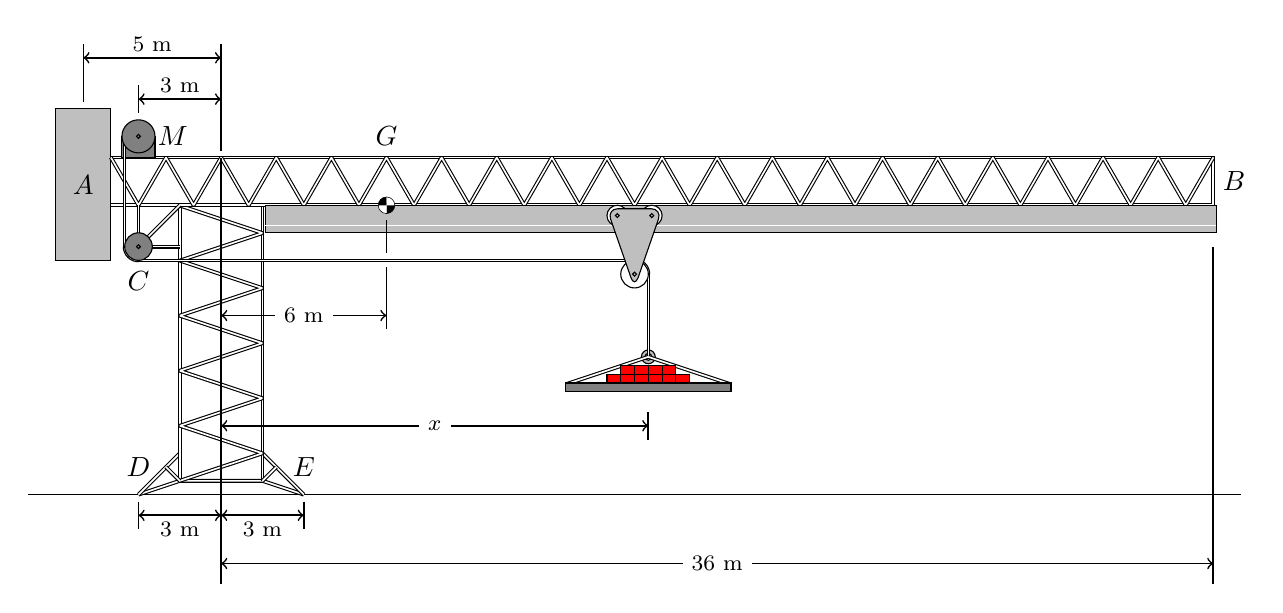
\begin{tikzpicture}[scale=0.35]
	\draw (-4,0) -- (40,0);
	\draw[double] (0,0) -- ++(1.5,0.5)--++(3,0)--++(1.5,-0.5);
	\draw[double] (0,0) -- ++(1.5,1.5) ++(3,0)--++(1.5,-1.5);
	\draw[double] (1.5,0.5) -- ++(0,10)--++(3,0)--++(0,-10);
	\draw[double,join=bevel] (1.5,0.5) -- ++(18.43:3.16) -- ++(161.57:3.16) -- ++(18.43:3.16) -- ++(161.57:3.16) -- ++(18.43:3.16) -- ++(161.57:3.16) -- ++(18.43:3.16) -- ++(161.57:3.16) -- ++(18.43:3.16) -- ++(161.57:3.16);
	\draw[double] (1.5,0.5) -- +(135:0.707);
	\draw[double] (4.5,0.5) -- +(45:0.707);
	\draw[fill=lightgray] (-1,8.5) rectangle (-3,14) node at +(1,-2.75) {$A$};
	\draw[double] (-1,10.5) -- ++(40,0) -- ++(0,1.732) -- ++(-40,0);
	\draw[double,join=bevel] (-1,10.5+1.732) -- ++(-60:2) -- ++(60:2) -- ++(-60:2) -- ++(60:2) -- ++(-60:2) -- ++(60:2) -- ++(-60:2) -- ++(60:2) -- ++(-60:2) -- ++(60:2) -- ++(-60:2) -- ++(60:2) -- ++(-60:2) -- ++(60:2) -- ++(-60:2) -- ++(60:2) -- ++(-60:2) -- ++(60:2) -- ++(-60:2) -- ++(60:2) -- ++(-60:2) -- ++(60:2) -- ++(-60:2) -- ++(60:2) -- ++(-60:2) -- ++(60:2) -- ++(-60:2) -- ++(60:2) -- ++(-60:2) -- ++(60:2) -- ++(-60:2) -- ++(60:2) -- ++(-60:2) -- ++(60:2) -- ++(-60:2) -- ++(60:2) -- ++(-60:2) -- ++(60:2) -- ++(-60:2) -- ++(60:2) node at +(0.75,-1.723/2) {$B$};
	\draw[fill=lightgray] (4.6,10.5) rectangle (39.1,9.5);
	\draw[double] (0,10.5) -- ++(0,-1.5) -- +(1.5,0);
	\draw[double] (0,9) -- +(45:2.121);
	\draw[fill=gray] (-0.6,13) rectangle (0.6,10.5+1.732);
	\draw[fill=lightgray, even odd rule] (18.5,5) circle (0.25) circle (0.125);
	\draw[double distance=0.4] (-0.5,13) -- ++(0,-4) ++(0.5,-0.5) -- ++(18,0) ++(0.5,-0.5) -- ++(0,-3);
	\draw (18,8.55) arc (90:0:0.55);
	\draw[fill=white] (18,8) circle (0.5);
	\draw[color=white] (4.6,9.75) -- (39.1,9.75);
	\draw[fill=white] (18.625,10.125) circle (0.375) +(-1.25,0) circle (0.375);
	\draw[rounded corners, fill=lightgray] (18,7.5) -- (19,10.375) -- ++(-2,0) -- cycle;
	\draw (18,8) circle (0.07);
	\draw (18.625,10.125) circle (0.07) +(-1.25,0) circle (0.07);
	\draw (-0.55,9) arc (180:270:0.55);
	\draw[fill=gray] (0,9) circle (0.5) circle (0.07) node at +(0,-1.25) {$C$};
	\draw[fill=gray] (0,13) circle (0.6) circle (0.07) node at +(1.25,0) {$M$};
	\draw[double] (18.5,5) -- +(3,-1) (18.5,5) -- +(-3,-1);
	\draw[fill=gray] (15.5,4.05) rectangle (21.5,3.755);
	\draw[fill=red] (17,4.06) rectangle +(0.5,0.3);
	\draw[fill=red] (17.5,4.06) rectangle +(0.5,0.3);
	\draw[fill=red] (18,4.06) rectangle +(0.5,0.3);
	\draw[fill=red] (18.5,4.06) rectangle +(0.5,0.3);
	\draw[fill=red] (19,4.06) rectangle +(0.5,0.3);
	\draw[fill=red] (19.5,4.06) rectangle +(0.5,0.3);
	\draw[fill=red] (17.5,4.37) rectangle +(0.5,0.3);
	\draw[fill=red] (18,4.37) rectangle +(0.5,0.3);
	\draw[fill=red] (18.5,4.37) rectangle +(0.5,0.3);
	\draw[fill=red] (19,4.37) rectangle +(0.5,0.3);
	%Dimensions
	\draw[semithick] (0,-0.25) -- +(0,-1) node at +(0,1.25) {$D$} ++(3,-3) -- +(0,3.25+10.5+1.723) ++(3,3) -- +(0,-1) node at +(0,1.25) {$E$} ++(33,-3) -- +(0,12.25);
	\draw[semithick] (3,10.75+1.732) -- (3,13.6+0.25+1+1.5) ++(-3,-1.5) -- +(0,-1);
	\draw[semithick] (-2,14.25) -- (-2,13.6+0.25+1+1.5);
	\draw[semithick] (9,6)--++(0,2.25) ++(0,0.5)--(9,9.95);
	\draw[semithick] (18.5,2) -- +(0,1);
	\fill (9,10.5) -- ++(0.3,0) arc (0:-90:0.3) -- ++(0,0.6) arc (90:180:0.3);
	\fill[white] (9,10.5) -- ++(0.3,0) arc (0:90:0.3) -- ++(0,-0.6) arc (270:180:0.3);
	\draw[very thin] (9,10.5) circle (0.3) node at +(0,2.5) {$G$};
	\draw[semithick, to-to] (0, -0.75) -- +(3,0) node[font=\footnotesize] at +(1.5,-0.5) {3 m};
	\draw[semithick, to-to] (3, -0.75) -- +(3,0) node[font=\footnotesize] at +(1.5,-0.5) {3 m};
	\draw[semithick, to-to] (3, -2.5) -- +(36,0) node[fill=white, font=\footnotesize] at +(18,0) {36 m};
	\draw[semithick, to-to] (3,13.6+0.25+0.5) -- +(-3,0) node[font=\footnotesize] at +(-1.5,0.5) {3 m};
	\draw[semithick, to-to] (3,13.6+0.25+2) -- +(-5,0) node[font=\footnotesize] at +(-2.5,0.5) {5 m};
	\draw[semithick,to-to] (3,6.5) -- +(6,0) node[fill=white, font=\footnotesize] at +(3,0) {6 m};
	\draw[semithick,to-to] (3,2.5) -- +(15.5,0) node[fill=white,font=\footnotesize] at +(7.75,0) {$x$};
	\end{tikzpicture}
	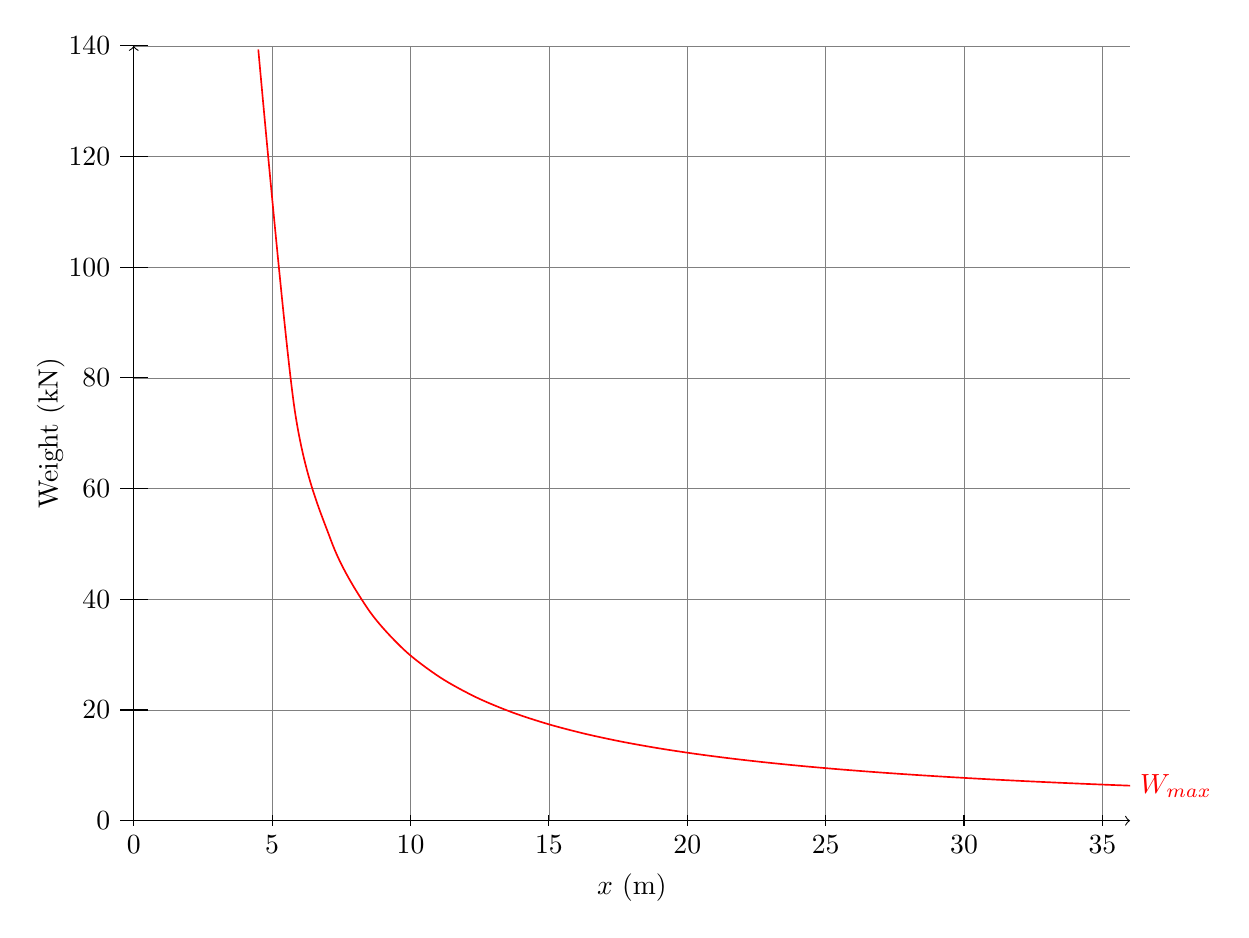
\begin{tikzpicture}[domain=0:36,x=100, y=20, scale=0.1]
	    \draw[very thin,color=gray] (0,0) grid[xstep=5,ystep=20] (36,140);
	    \foreach \x in {0,5,...,35}
	        \draw (\x,1) -- (\x,-1)
	            node[anchor=north] {\x};
	\foreach \y in {0,20,...,140}
	        \draw (0.5,\y) -- (-0.5,\y)
	            node[anchor=east] {\y};
	    \draw[->] (0,0) -- (36,0) node at +(-18,-12) {$x$ (m)}; 
	    \draw[->] (0,0) -- (0,140) node[rotate=90] at +(-3,-70) {Weight (kN)};
	    \draw[color=red,domain=4.5:36, smooth, semithick] plot (\x,{209/(\x-3)}) node[right] {$W_{max}$};
	\end{tikzpicture}
	
	\subsection{Ballistics }
	\textbf{Definition (\#\mydef):} "\NewTerm{Ballistics}\index{ballistics}" is the science or study of the motion path of a body having an initial velocity through a given medium in space immersed in a given (most of time: constant) field (gravitational, magnetic or electrostatic).
	
	\begin{tcolorbox}[title=Remarks,colframe=black,arc=10pt]
	We have hesitate, and still do, to write this subject in the section of Spatial Engineering. So it is not impossible that in a near of or far future this subject moves in another section.
	\end{tcolorbox}
		
	We will prove now thanks to our knowledge in kinematics that the parabolic movement is the natural movement of a mobile body in the field of gravity in empty space animated (without friction or where friction can be neglected) by a travel speed $\vec{v}_0$  not necessarily parallel to the acceleration of gravity $\vec{g}$ (in general this is therefore a curvilinear motion ). For example, a projectile having an initial velocity $\vec{v}_0$ inclined from an angle $\beta$ from the horizontal:

	\begin{figure}[H]
		\centering
		\includegraphics{img/mechanics/ballistics.jpg}
		\caption{Ballistics configuration study}
	\end{figure}
	And with some vocabulary stuff associated:
	\begin{figure}[H]
		\centering
		\includegraphics{img/mechanics/ballistics_vocabulary.jpg}
		\caption[]{Typical Artillery vocabulary in ballistics}
	\end{figure}
	Obviously the reader can ask himself if the study of ballistics is useful outside artillery?! In fact even if does not apply to rocket launch as their velocity is not constant (boosters) and the application to golf is not quite interesting for engineers we have some practical situation where surch calculations are useful. A contemporary one is "ice ballistic problem" for the security radius around wind turbine to avoid people or houses to receive blocks of ice (in winter) that detach from the pales in rotation at a given rotation speed $\omega$ and for sure the trajectory if this ice is a ballistic trajectory!!! 
	
	In the absence of gravity and friction the mobile $P$ would follow the straight departure line indefinitely. The action of the gravity is to take it down, at time $t$, of the well known value to us $\dfrac{1}{2}gt^2$.

	We put the projection on the axes:
	
	combination of smooth movement along the $x$-axes and a falling motion with initial velocity $v_{0y}$ along the $y$-axes. Which corresponds to the following equations:
		
	eliminating the time between these two equations we get the path (equation of a parabola):
		
	which had already been obtained by Galileo in the early 17th century.

	We calculate also the target range $x_{\max}$ of the projectile by putting $y=0$ in the above equation and we get easily:
		
	the solution $x=0$ have no interest.

	The maximum height $y_{\max}$ can be calculated by canceling the derivative of the equation of the trajectory. So we get easily:
	
	We notice that for the maximum range for a given initial speed we have two typical cases to consider:
	\begin{enumerate}
		\item We give ourselves and unreachable target range $x_{\max}$ as it is not possible that $\sin(\beta)>1$.

		\item As we have $\sin(2\beta)$ in the expression of $x_{\max}$ it is obvious that it is $\beta=\pi/4$ ($45^\circ$) that gives the maximum range of a give initial speed.
	\end{enumerate}
	The curve enveloping all parables, plotted for a given initial speed $v_0$ in all possible directions, is still a parable named "\NewTerm{safety parabola}\index{safety parabola}". Its rotation about the $y$-axis creates a paraboloid which circumscribes (contains) the region of the space accessible only to projectiles.
	\begin{figure}[H]
		\centering
		\includegraphics{img/mechanics/safety_parabola.jpg}
		\caption[]{Ballistic safety parabola}
	\end{figure}
	Thus, it is not too difficult to find the equation of this safety parabola :

	The vertically shot ($\beta=\pi/4$) is known to us and is given by:
	
	The maximal range is as we know given by:
	
	So when $x=x_{\max}\Rightarrow y=0$ such that:
	
	which is the equation of the safety parabola.
	
	The time of flight is the time it takes for the projectile to finish its trajectory. As we have for the vertical component:
	
	and the "\NewTerm{time of flight}\index{time of flight}" is given when $y=0$, it comes therefore:
	
	That is to say:
	
	The "\NewTerm{angle of reach}\index{angle of reach}" is the angle $\beta$ at which a projectile must be launched in order to go a distance $x_{\max}$, given the initial velocity $v_0$. So from:
	
	We get:
	
	Ok now much more interesting... To hit a target at range $x_T$ and altitude $y_T$ when fired from $(0,0)$ and with initial speed $v_0$ the required angle(s) of launch $\theta$ are:
	
	The two roots of the equation correspond to the two possible launch angles, so long as they aren't imaginary, in which case the initial speed is not great enough to reach the point $(x,y)$ selected.
	\begin{dem}
	First, let us recall that:
	
	Solving the first for $t$ and substituting this expression in the second gives (using the trigonometric identities proved in the section of Trigonometry):
	
	After a small rearrangement:
	
	Let us put $\Gamma=\tan(\beta)$:
	
	Solving this second order polynomial as we learned to do it in the section Calculus we have for discriminant:
	
	So we get after simplifications:
	
	Hence:
	
	If instead of a coordinate $(x,y)$ it is required to hit a target at distance $r$ and angle of elevation $\theta$  (polar coordinates), we use the relations $x_T=r_T\cos(\theta_T), y_T=r_T\sin(\theta_T)$  and substitute to get:
	

	\begin{flushright}
		$\square$  Q.E.D.
	\end{flushright}
	\end{dem}
	
	\pagebreak
	\subsection{Kinematics of Circular Motion}
	The motion of objects as they translate -- move bodily from one place to another -- follows a simple set of rules. It turns out that a very similar set of rules describes the motion of objects as the rotate -- spin around in place.

	Most situations we have considered so far involve the type of motion named "translation" (pick it up and put it down somewhere else).

	But centrifuges, planets, space stations, satellites, molecules, motor engines exhibit a different sort of motion: rotation (spit in in place)!

	The circular movement, also named "\NewTerm{rotation movements}\index{rotation movements}", thus describe the rotation of an object around an axis (or a point to make simpler). The usage is to define it with the following information:

	\begin{itemize}
		\item The direction of the axis of rotation plane in space

		\item The direction of rotation on the constant radius circle around this axis

		\item The speed $v$ on the circular path.
	\end{itemize}
	All this can be resumed in the following figure:
	\begin{figure}[H]
		\centering
		\includegraphics{img/mechanics/circular_motion_principle.jpg}
	\end{figure}
	where for:
	
	we have used the relation prove in the section of Trigonometry (it is just logical by definition if the angle is measured in radians):
	
	We summarize these three directions by the data give by a vector "\NewTerm{instantaneous angular velocity}\index{instantaneous angular velocity}":
	
	The direction of rotation is said to be "positive" when the thumb drawn in the direction of the unit vector $\vec{n}$, we take the axis of the right hand and one sees the object rotate in the direction of the other four fingers ("\NewTerm{right hand rule}\index{right hand rule}"):
	\begin{figure}[H]
		\centering
		\includegraphics[scale=0.5]{img/mechanics/right_hand_rule.jpg}
		\caption{Right Hand Rule (source: Wikipedia)}
	\end{figure}
	The norm of the instantaneous angular speed, represents obviously the angle traveled per unit of time,by the object that moves in the plane perpendicular to the unit vector $\vec{n}$:
	
	
	Of course, it goes without saying that the angular velocity is given in radians per second and not in revolutions per minute or degrees per second!!! We must therefore be careful to always do the right conversion!
	
	\begin{tcolorbox}[title=Remarks,colframe=black,arc=10pt]
	\textbf{R1.} In the general case of the circular motion, angular velocity of the object studied varies over time: $\omega=\omega(t)$.\\
	
	\textbf{R2.} When the direction of the rotation axis changes, the components of unit vector $\vec{n}$ are functions of time. This is the case of a motorcycle wheel in a turn for example.
	\end{tcolorbox}
	If $\mathrm{d}t$ is the time required for this movement, the curvilinear velocity of the point is therefore:
	
	then we fall back on the result already given previously.
	
	Now let us do the same that during our study of the rectilinear uniform movement and let us determine the angular position over time. Then we have:
	
	Therefore:
	
	and if $t_0=0$, then we have:
	
	to be compared with the equivalent relation between position and speed obtained during our study of rectilinear kinematics.
	
	Now let us consider the definition of "\NewTerm{angular acceleration}\index{angular acceleration}" (the traditional notation is a bit unfortunate ...):
	
	Then we have:
	
	and therefore:
	
	 and if $t_0=0$, then we have:
	
	What we can write:
	
	Therefore it comes:
	
	Hence:
	
	and if $t_0=0$, then we have:
	
	compared with the equivalent relation between position, velocity and acceleration obtained in our study of the straight kinematics.

Let us now look to the vector of circular motion which will be extremely important one step further and also in many other chapters. So give us a Euclidean orthonormal such as:
	\begin{figure}[H]
		\centering
		\includegraphics{img/mechanics/kinematics_circular_motion_vector_analysis.jpg}
	\end{figure}
	We see well from the above figure that:
	
	So finally we have:
	
	We see then that we are dealing with a cross product (\SeeChapter{see section Vector Calculus}) such that:
	
	So we have:
	
	that we also write:
	
	The acceleration of the circular motion is therefore is formed in the general case, of two terms, the first being the "\NewTerm{tangential acceleration}\index{tangential acceleration}" always expressing the variation of the speed along the path and the second acceleration perpendicular along the named "\NewTerm{normal acceleration}\index{normal acceleration}" or "\NewTerm{centripetal acceleration}\index{centripetal acceleration}" (centripetal meaning: "that tends to bring the center"). This is why the normal acceleration is also sometimes denoted by  $\vec{a}_c$.
	
	\begin{tcolorbox}[title=Remark,colframe=black,arc=10pt]
	Following Newton's second law we can associate a force to each of this both acceleration. However there must be no confusion between: "\NewTerm{centrifugal force}\index{centrifugal force}" (Latin for "center fleeing") that describes the tendency of an object following a curved path to fly outwards, away from the center of the curve. It's not really a force; it results from inertia — the tendency of an object to resist any change in its state of rest or motion, and the "\NewTerm{centripetal force}\index{centripetal force}" that is a real force that counteracts the centrifugal force and prevents the object from "flying out," keeping it moving instead with a uniform speed along a circular path.
	\end{tcolorbox}
	\begin{tcolorbox}[colframe=black,colback=white,sharp corners]
	\textbf{{\Large \ding{45}}Example:}\\\\
	The centrifugal "force" on Earth's equator is equal to:
	
	To compare at the same place to Earth's gravitation force that is of $F_G=9.800\;[\text{m}\cdot \text{s}^{-2}]$. The resultant is then $F_G=9.766\;[\text{m}\cdot \text{s}^{-2}]$.
	\end{tcolorbox}
	The reader interested to vector expressions of the speed and acceleration in cartesian, polar, cylindrical and spherical coordinates should refer to the section of Vector Calculus where all the details ar given where we get for recall:

	\begin{itemize}
		\item In cartesian coordinates:
			\begin{itemize}
				\item Velocity:
								
	
				\item Acceleration:
				
			\end{itemize}

		\item In polar coordinates:
			\begin{itemize}
				\item Velocity: 
				
	
				\item Acceleration: 
				
			\end{itemize}
		
		\item In cylindrical coordinates:
			\begin{itemize}
				\item Velocity:
				
	
				\item Acceleration:
				
			\end{itemize}
			
		\item In spherical coordinates:
			\begin{itemize}
				\item Velocity:
				
	
				\item Acceleration:
				
			\end{itemize}
	\end{itemize}
	For the details of the analysis of the velocity and acceleration of a elliptical motion the reader should refer to the section of Astronomy.
	
	Also from the vis-viva equation proved in the section of Aerospace Engineering we get the speed of a body in any point of an ellipse:
	
	where as proved in the section of Analytical Geometry:
	
	where $a$ is the semi-major axis of the ellipse.
	
	For non-planar and not rectilinear motions (that is to say: the generalization of what we have seen so far). The reader should refer to the section of Differential Geometry.
	
	If we express the circular movement of a point $P$ from a system of axes lying in the plane of the trajectory, for simplicity, then the position of the point $P$ is given by parametrically by (\SeeChapter{see section Analytical Geometry}):
	
	This shows that the circular movement can be considered as the superposition of two sinusoidal  movements phase-shifted of $\pi/2$. But if we write now more generally we could also have:
	
	Or even more general:
	
	or more general again:
	
	we get by focusing on on the coordinates:
	
	by varying the phase difference $\varphi$ and the ratio $\omega_x/\omega_y$ we get curves that we name "\NewTerm{Lissajous figures}\index{Lissajous figures}":
	\begin{figure}[H]
		\centering
		\includegraphics{img/mechanics/lissajous_figures.jpg}
		\caption{Lissajous figures}
	\end{figure}
	An important case to consider for the study of circular particles accelerators is the acceleration vector of a uniform circular movement. For such a movement, the position vector in time $t$ is obviously given by:	
	
	where $R$ is the radius, $\omega$ the (constant) angular velocity and $\vec{e}_x$,$\vec{e}_y$ the orthonormal unit vectors for $x$ and $y$.

	The acceleration vector being given by:
	
	Carry out the two derivations we find:
	
	Therefore:
	
	So in uniform circular motion the only acceleration vector always points opposite to the position vector, to the center of the trajectory.
	
	The reader will find very important practical applications of the kinematics of the circular motion to for the industry relatively to mechanics in the section of Mechanical Engineering (\SeeChapter{see chapter Engineering}) and also to Astronomy (\SeeChapter{see chapter Cosmology}) and to Corpuscular Quantum Physics (\SeeChapter{see chapter Atomistic}).
	
	\pagebreak
	\subsection{Energy, Work and Power}
	When a force acts upon an object to cause a displacement of the object, it is said that work was done upon the object. There are three key ingredients to work - force, displacement, and cause. In order for a force to qualify as having done work on an object, there must be a displacement and the force must cause the displacement. There are several good examples of work that can be observed in everyday life - a horse pulling a plow through the field, a father pushing a grocery cart down the aisle of a grocery store, a freshman lifting a backpack full of books upon her shoulder, a weightlifter lifting a barbell above his head, an Olympian launching the shot-put, etc. In each case described here there is a force exerted upon an object to cause that object to be displaced.
	
	If a mass point $m$ undergoes an elementary displacement $\mathrm{d}\vec{r}$ under the effect of a force $\vec{F}$, this force performs an elementary work $W$ given by definition by the "\NewTerm{work equation}\index{work equation}":
	
	However the reader must be careful. It's now why a body accelerates (begin to move) that there is necessarily a force!!! Indeed, Einstein has proved that what we have consider for centuries as the "gravitational force" was in fact only a body following the space-time curvature. So never go too quick in conclusion we making science...
	
	On occasion, a force acts upon a moving object to hinder a displacement. Examples might include a car skidding to a stop on a roadway surface or a baseball runner sliding to a stop on the infield dirt. In such instances, the force acts in the direction opposite the objects motion in order to slow it down. The force doesn't cause the displacement but rather hinders it. The negative work refers obviously to the numerical value that results when values of $F$, $d$ and $\theta$ are substituted into the work equation. Since the force vector is directly opposite the displacement vector, theta is $\pi$ degrees. The $\cos(\pi)$ is $-1$ and so a negative value results for the amount of work done upon the object.
	
	\textbf{Definition (\#\mydef):} If the work $W$ is positive the work is named "\NewTerm{engine work}\index{engine work}". If negative we speak then of "\NewTerm{resistive work}\index{resistive work}".
	
	If the mass $m$ moves from a point $A$ to place $B$, the total work is:
	
	For the units we have the express either in "\NewTerm{Joules [J]}\index{Joules}" given by:
	
	The definition above we can also quickly deduce the work of a moment of force (or in other words, the work of a force in a rotational movement) because of an infinitesimal element of movement, we have:
	
	So in the case of circular motion the work of a moment of force will be given by:
	
		
	\subsubsection{Conservative vector field}
	If the force $\vec{F}$ is constant in magnitude and in direction (gravity near the Earth's surface for example), the integral calculation of $W$ takes a simpler form:
	
	This result shows that the work depends only the initial and final positions and not of the path traveled in this special condition. 
	
	But in fact there is a more general result that we have already proved proved in the section of Differential and Integral Calculus that is the "\NewTerm{fundamental theorem for line integrals}\index{fundamental theorem for line integrals}" or "\NewTerm{gradient theorem for line integrals}\index{gradient theorem for line integrals}" that gives us:
	
	where $\vec{\nabla}()$ is the gradient operator (\SeeChapter{see section Vector Calculus}).
	
	The force of gravity, of electrostatic force is a special case of this type but in fact in all situations as it derives from a potential (see details further below)!
	
	A "\NewTerm{conservative vector field}\index{conservative vector field}" (also named a "\NewTerm{path-independent vector field}\index{path-independent vector field}") is a vector field $\vec{F}$ whose line integral $\oint_\Gamma \vec{F}\circ\mathrm{d}\vec{r}$ over any curve $\Gamma$ depends only on the endpoints of $\Gamma$. Therefore a vector field for which we have:
	
	is by definition automatically a conservative vector field and then we say that there is "no circulation around a closed curve".
	
	We have also proved in the section of Vector Calculus the Stokes theorem that gives for recall a simply connected domain, a continuously differentiable vector field $\vec{F}$ :
	
	Therefore for a conservative vector field:
	
	So a vector field that is continuously differentiable on a simply connected domain such that:
	
	is also a possible criteria of identification of a conservative vector field.
	
	\begin{tcolorbox}[colframe=black,colback=white,sharp corners]
	\textbf{{\Large \ding{45}}Example:}\\\\
	Our goal is to determine if the vector vield
	
	is conservative or not.

	One condition for path independence is as we know the following: for a simply connected domain, a continuously differentiable vector field $\vec{f}$ is path-independent if and only if its curl is zero.
	
	Then we have:
	
	We calculate:
	
	Since these partial derivatives are equal, the curl is zero.\\

	van we conclude $\vec{F}$ is conservative? The problem is that$\vec{F}$ is not defined at the origin $(0,0)$. Its domain of definition has a hole in it, which for two-dimensional regions, is enough to prevent it from being simply connected. The test does not apply, and we still don't know whether or not $\vec{F}$ is conservative.\\
	
	Let's try another test, this time a test for path-dependence. If we can find a closed curve along which the integral of $\vec{F}$ is nonzero, then we can conclude that $\vec{F}$is path-dependent. If the curve does not go around the origin, then we can use Green's theorem (\SeeChapter{see section Vector Calculus}) as we have only the third component of the curl that was non-null above:
	
	to show the integral of $\vec{F}$ is zero or not using path integral rather than directly the curl.\\
	
	We choose for closed path a circle and then we can use a reparametrization of the field using $x= \cos(t)$ and $y=\sin(t)$ with $0\leq t\leq 2\pi$. Then on the unit circle, $\vec{F}$ takes a simple form:
	\end{tcolorbox}
	
	\begin{tcolorbox}[colframe=black,colback=white,sharp corners]
	
	and we have obviously:
	
	Therefore:
	
	The hole in the domain at the origin did end up causing trouble. We found a curve $\Gamma$ where the circulation around $\Gamma$ is not zero. The vector field $\vec{F}$ is therefore path-dependent.
	\end{tcolorbox}
	The relation:
	
	is sometimes named "\NewTerm{theorem of kinetic energy}\index{theorem of kinetic energy}" or "\NewTerm{work-energy theorem}\index{work-energy theorem}".

	Note that in the case of a rectilinear movement, to which a mobile initially at rest travels a distance $d$ distance being subjected to a certain force, we (omitting course the change in potential energy and energy loss by friction):
	
	that we name "\NewTerm{working force}\index{working force}".
	
	\subsubsection{Kinetic Energy}
	Newton's second law $\vec{F}=m\vec{a}$ applies along a path $A$-$B$. By using the expression of the work we have:
	
	and by developing the dot product using the components we have:
	
	By definition we say that each term in the last equality is the (non-relativistic) "\NewTerm{kinetic energy}\index{kinetic energy}" denoted by:
	
	and it is measured in obviously also in Joules [J] (or other exotic derivate units whose theoretical physicists sometimes abuse a little bit too much...) and is always positive in mechanics or any other field of physics.

	The previous development can then be rewritten as:
	
	Therefore when a body moves (without rotation on itself) under the action of any force $\vec{F}$, the work of this acceleration force on any path $A$, $B$ is equal to the change in kinetic energy of the body.
	
	\paragraph{Moment of inertia}\mbox{}\\\\
	The "\NewTerm{moment of inertia}\index{moment of inertia}", otherwise known as the "\NewTerm{angular mass}\index{angular mass}" or "\NewTerm{rotational inertia}\index{rotational inertia}", of a rigid body determines the torque needed for a desired angular acceleration about a rotational axis. It depends on the body's mass distribution and the axis chosen, with larger moments requiring more torque to change the body's rotation. 

	For bodies constrained to rotate in a plane, we will see that is sufficient to consider their moment of inertia about an axis perpendicular to the plane. For bodies free to rotate in three dimensions, their moments must be described by a symmetric $3\times 3$ matrix; each body has a set of mutually perpendicular principal axes for which this matrix is diagonal and torques around the axes act independently of each other.
	
	To a rigid solid rotating about an axis at the angular velocity $\vec{\omega}$, the elementary kinetic energy of any point of mass $\mathrm{d}m$, located off-axis, is:
	
	since $\vec{\omega}$ and $\vec{r}$ are perpendicular. The total kinetic energy is then:
	
	We have become accustomed in physics to writh this last relation:
	
	with the "\NewTerm{moment of inertia}\index{moment of inertia}" defined by:
	
	\begin{tcolorbox}[colframe=black,colback=white,sharp corners]
	\textbf{{\Large \ding{45}}Examples:}\\\\
	E1. Let us calculate the final velocity of a rigid ball falling on an incline rigid plane with nonzero friction (therefore the ball is going to rotate) in a gravitational potential field where the friction heat can be neglected and in vacuum.\\

	The answers of of the beginner will often be obtained by considering only the kinetic energy but not the rotating speed of the ball. Now we must take this into account through its moment of inertia.\\

	So we have the total kinetic energy that the translation kinetic energy of the center of mass plus the rotational energy around the same center of mass:
	
	\begin{figure}[H]
		\centering
		\includegraphics{img/mechanics/rotating_ball_inclined_plane.jpg}
	\end{figure}
	equaling that value with that of the gravitational potential energy (see further below), assuming a zero initial velocity of fall, we have:
	
	Thus we get the velocity acquired at the bottom of the plane (rolling friction not included...):
	
	and we have proved in the section of Geometric Shapes that the moment of inertia of a solid ball around its center of mass is:
	\end{tcolorbox}
	
	\begin{tcolorbox}[colframe=black,colback=white,sharp corners]
	
	Therefore it comes:
	
	We see in the special case of the ball, that final speed of drop is (without air friction and without energy loss due to friction) independent of its mass and radius and of then angle of the plane (whether the ball is empty or full) which is relatively counter-intuitive.\\
	
	E2. A second famous example is the calculation of the rotational kinetic energy of a perfectly spherical planet of homogeneous mass and constant rotational period. Then we have:
	
	\end{tcolorbox}
	In a solid, the distribution of the material about an axis will obviously be different depending on the chosen axis. The moment of inertia corresponding will also be obviously different. It is therefore essential to specify the axis with respect to which we wish to determine the moment of inertia. We see that in practice that engineers often place the axis so that it passes through the center of mass. In the tables, we frequently find expressions of inertia moments of common forms (along a given axis) such as cylinder, cone, sphere, bar, tube.
	
	Here is a summary of some moment of inertia of plane figures among all those proved in detail in the section of Geometric Shapes:
	\begin{figure}[H]
		\centering
		\includegraphics{img/mechanics/moment_inertia_plane_shapes.jpg}
	\end{figure}
	and same for some body (volumic) shapes (proofs are also available in the same section):
	\begin{figure}[H]
		\centering
		\includegraphics{img/mechanics/moment_inertia_body_shapes.jpg}
	\end{figure}
	We saw in our study of angular momentum that:
	
	and just before that the moment of inertia is given by:
	
	So we have:
	
	hence:
	
	We finally get:
	
	it is the expression of the angular momentum of a rigid body rotating on itself (on one of its possible axes of rotation).
	
	As we showed during our study of the angular momentum:
	
	then it comes under the assumption that the mass and geometry of the solid remain constant ... that the moment of force is then:
	
	And obviously, if we study a system in which the angular momentum is conservative, it is obvious that:
	
	This conservation of angular momentum is applicable in a multitude of experiences as the well known which is to turn on a chair and spread out hands or legs which will decrease the speed (and vice versa) as illustrated in figure below:
	\begin{figure}[H]
		\centering
		\includegraphics{img/mechanics/angular_momentum_moment_of_inertia_conservation_1.jpg}
		\caption{Conservation of the angular momentum on variation of inertia momentum}
	\end{figure}
	Another curious experience (but mathematically correct) to take place ourselves on a turntable with a wheel in rotation held horizontally (vertical angular momentum is zero) and put it then vertically (same type of experiment can be done in the opposite direction). As the vertical momentum must remain zero to counteract this (or must remain constant in direction and in amplitude as it is a vectorial quantity), the plateau on which is put the experimenter will rotate in the opposite direction of rotation of the wheel.
	\begin{figure}[H]
		\centering
		\includegraphics{img/mechanics/angular_momentum_moment_of_inertia_conservation_2.jpg}
		\caption{Conservation of total angular momentum by variation of intern angular momentum}
	\end{figure}
	\begin{tcolorbox}[title=Remark,colframe=black,arc=10pt]
	The movement of large masses on the surface of the Earth (icebergs, river flooding, tectonic plates, etc.) cause changes in moment of inertia of the Earth. It follows therefore fluctuations of the angular velocity and therefore imperfection of astronomical time standard (a few thousandths per day).
	\end{tcolorbox}
	Now let us come back to the methods of calculation of the moments of inertia. The kinetic energy of a body is the sum of kinetic energy of each element of this body at the macroscopic level, then we have:
	
	Therefore in the context of a solid rigid body rotating around an axis, we have:
	
	Thus, for a body composed of a plurality of different geometries, the total moment of inertia is the sum of the moments of inertia with respect to the axis of rotation of each of the sub-geometries such that:
	
	When we calculate the moment of a body of inertia relative to a given axis $\Delta$ of rotation, it may be interesting to know what is the distance from the axis where we can place fictitiously the whole mass of this body concentrated on a given point for the same moment of inertia. By definition, this distance denoted $k$ and named the "\NewTerm{radius of gyration}\index{radius of gyration}" is trivially given by:
	
	where $J_\Delta$ is the known moment of inertia of the body of mass $M$ relatively to an axis $\Delta$.
	
	By definition, the "\NewTerm{polar moment of inertia}\index{polar moment of inertia}" (or also "\NewTerm{squared moment of inertia}\index{squared moment of inertia}") is the moment of inertia defined with respect to a point (a "pole") and not relatively to an axis and written:
	
	This quantity intervene only for free spins and is of interest, for rotations around a fixed axis, only because it sometimes facilitates the calculation of the axial moments of inertia under the follows relation (in Cartesian coordinates):
	
	\begin{dem}
	\begin{lemma}
	The moment of inertia compared to the $x$O$y$ plane is trivially given by:
	
	\begin{figure}[H]
		\centering
		\includegraphics{img/mechanics/inertia_polar_momentum_lemma1.jpg}
	\end{figure}
	\end{lemma}
	\begin{lemma}
	The moment of inertia with respect to an axis is given by:
	
	\begin{figure}[H]
		\centering
		\includegraphics{img/mechanics/inertia_polar_momentum_lemma2.jpg}
	\end{figure}
	\end{lemma}
	Summing these relations, we deduce:
	
	The polar moment of inertia is then given by:
	
	\begin{figure}[H]
		\centering
		\includegraphics{img/mechanics/inertia_polar_momentum_proof.jpg}
	\end{figure}
	Comparing with Lemma 2 we get:
	
	\begin{flushright}
		$\square$  Q.E.D.
	\end{flushright}
	\end{dem}
	If the body in question has a spherical symmetry, it comes immediately as $J_x=J_y=J_z:J$ that:
	
	An example is given with the ball (full sphere) in the section on Geometric Shapes in the chapter Geometry.
	
	If the body in question has a spherical symmetry, it comes immediately as $J_x=J_y=J_z:=J$ that:
	
	An example is given with the ball (full sphere) in the section on Geometric Shapes in the chapter Geometry.
	
	Suppose now that we know the moment of inertia $J_z$ of a rigid solid body compared to any other perpendicular axis (the chosen axis is not necessarily only assimilated to the common $z$ axis) passing through the center of mass $G$. Then let us calculate the moment of inertia $J_z$, relatively to another axis $z'$, parallel to  $z$ and remote from distance $d$, and let us make up appear the existing link between these two different moments of inertia.
	
	So consider the following figure representing our subject of interest:
	\begin{figure}[H]
		\centering
		\includegraphics[scale=0.6]{img/mechanics/parallel_axis_theorem_huyghens_steiner.jpg}
	\end{figure}
	 In a planar Cartesian reference frame, we have for any points $(x, y)$:
   
   and:
   
   Then we have:
   
   and:
   
   The therm:
    
   is zero because if the moment of inertia is calculated relatively to the center mass $G$ as we have assumed it from the beginning, then:
   
   Ultimately, we finally get the "\NewTerm{Huygens-Steiner theorem}\index{Huygens-Steiner theorem}" also named "\NewTerm{parallel axis theorem}\index{parallel axis theorem}":
   
    As we will see it in the section on Geometric Shapes in the chapter Geometry, it then becomes easy to calculate the moment of inertia of an equilateral triangle knowing that of a square plate and moving the axis inertia to the point where the triangle is the center of gravity (ie at the third of the median between the center of the rectangle and of its vertices).

   Since there are as many moments of inertia as axes of rotation and that they are often in practical study cases related to the principal axes of inertia (axis related to the axes of revolution or symmetry planes - see below), it may be useful to introduce a mathematical being useful in the context of representation of moments of inertia which is none other than the "\NewTerm{inertia matrix}\index{inertia matrix}" or also known as (modern formulation) "\NewTerm{inertia tensor}\index{inertia tensor}".
   
   The approach to rigorously determine the expression of this tensor is the following: 

   Given $A_i$ a given point of a solid, for which we seek to calculate the moment of inertia and $\Delta$ the axis of origina O and vector of unit vector $\vec{u}$ relative to which we wish to calculate the moment of inertia. Any point $A_i$ of the solid can be projected (orthogonal projection) on a point $H\in \Delta$ from the knowledge of the angle $\theta$ between $\Delta$ and $\overrightarrow{\text{O}A_i}$ such that:
    
   Therefore:
   Therefore:
   
   Based on the properties of the mixed product (\SeeChapter{see section Vector Calculus}) and of the scalar product:
   
   we have:
   
   and therefore:
  
  As $\vec{u}$ is a vector of constant direction whatever the point of integration, we can take it out of the integral such that:
   
   We can check that if we replace $\vec{u}$ by $\vec{u}_1+\vec{u}_2$, we will get a result that also sum (of the type $\vec{v}=\vec{v_1}+\vec{v}_2$ that is the sum of two integrals) up by the property of linearity  of the cross product (\SeeChapter{see section Vector Calculus}). 

   Therefore, the application that to $\vec{u}$ associated a given $\vec{v}$ is therefore a linear application that can be represented in a given basis $\mathcal{B}$ by a matrix:
   
   The matrix $[J_0]_{\mathcal{B}}$ is named "\NewTerm{inertia tensor}\index{inertia tensor}" of the system relatively to the point O, in the base $\mathcal{B}$.

  The moment of inertia of a system with respect to any axis $\Delta$ of unit vector $\vec{u}$ is given by:
  
  The problem now is to calculate the elements of the tensor $[J_0]$ for a given basis $\mathcal{B}$. Given a reference frame $(\text{O},\vec{i},\vec{j},\vec{k})$ such that $\text{O} \in \Delta$ we put:
   
   and:
    
   Using the fact that we know that a cross product can be represented by a assymetric matrix (\SeeChapter{see section Vector Calculus}):
   
   and therefore:
   
	In the above expression of the inertia matrix, we recognize the diagonal elements: it is simply the moments of inertia of the system relatively to the different axes of the base. We name "\NewTerm{product of inertia}\index{product of inertia}" the non-diagonal elements of the matrix and we write them:
   
   Therefore we have:
   
    where obviously:
   \begin{itemize}
       \item $J_{\text{O}x}$ is the inertial momentum relatively to $(\text{O},\vec{x})$
        \item $J_{\text{O}y}$ is the inertial momentum relatively to $(\text{O},\vec{y})$
        \item $J_{\text{O}z}$ is the inertial momentum relatively to $(\text{O},\vec{z})$
        \item $J_{yz}$ is the inertial momentum relatively to $(\vec{y},\vec{z})$
        \item $J_{xz}$ is the inertial momentum relatively to $(\vec{x},\vec{z})$
        \item $J_{xy}$ is the inertial momentum relatively to $(\vec{x},\vec{y})$
   \end{itemize}
   Also sometimes written as (USA notation and mechanical engineers notation):
   
   If O is assimilated to the center of mass of the solid, we simply write:
   
   It follows if thickness of the study body is negligible compared to the other dimensions then $z=0$ and then we have immediately:
   
   We can also generalize Huygens theorem by making use this matrix. To do so, let us write $(x', y', z')$ the coordinates of any point $A$ in $R'$ and $(x, y, z)$ its coordinates in $R$. We write $(a, b, c)$ the coordinates of the O' of $R'$ in $R$:
	
   as:
   
   We then have:
   
   Now if O' coincides with the center of mass $G$, then according to the definition of the center of mass:
   
   We deduce then:
   
   and also:
   
   with:
   
   We fall back on the classic Huygens theorem since $a^2+b^2$ is none other than the squared distance between the axis O$z$ and $Gz$ and same for $b^2+c^2$ that is the squared distance between O$x$ and $Gx$ and $a^2+c^2$ which is the distance between O$y$ and G$y$.
   
   If we now focus on the products of inertia, we get:
   
   Therefore, if O' coincide with $G$:
   
   In summary, the "\NewTerm{Huygens generalized theorem}\index{Huygens generalized theorem}" is written:
   
   The inertia tensor being real and symmetric, we have proved in the section of Linear Algebra (spectral theorem) that it is always possible to find three perpendicular directions of vectors $\vec{e}_1,\vec{e}_2,\vec{e}_3$ such as the symmetrical  tensor (matrix) is diagonalisable:
   
   The trihedron formed by the vector $\vec{e}_1,\vec{e}_2,\vec{e}_3$ is named "\NewTerm{main trihedron of inertia}\index{main trihedron of inertia}" and its axes are named "\NewTerm{principal axes of inertia}\index{principal axes of inertia}". In this reference frame $[J_0]$ takes the name of "\NewTerm{principal inertia tensor}\index{principal inertia tensor}". If furthermore O is assimilated to $G$, we speak of "\NewTerm{central tensor of inertia}\index{central tensor of inertia}".
   
   In fact, to find the moments of inertia relatively to the principal axes it is almost never necessary to diagonalise the inertia tensor because it is often enough to be guided by the symmetry of the system. We'll see the following theorems that if there are axes or planes of symmetry for the mass distribution, the axes of inertia are easy to find. In addition, the system is generally simple enough (or sufficiently broken down into simple elements ...) for these axes to be obvious.
    \begin{theorem}
    If the system has a material plane of symmetry (ie: $\rho(A)=\rho(A')$ if $A$ is the symmetric of $A'$ relatively to the plane) then any axis perpendicular to this plane is a principal axis of inertia and therefore the inertia matrix reduce to:
    
    \end{theorem}
    \begin{dem}
    Let us choose a reference frame $x\text{O}y$ in the plane relatively to which the system has a mass distribution that is symmetrice and O$z$ an axis perpendicular to this plane. To calculate $\int xz\mathrm{d}m$ or $\int yz\mathrm{d}m$ let us group the points by pairs, symmetrical to $x\text{O}y$. that is to say such that $z_A=-z_{A'}$. We then have:
     
      and even:
      
      that is to say, as (material symmetry!):
      
     that all contributions of symmetrical paires of points are zero, which implies:
    
    that is to say, the $z$ axis is a main direction of inertia.
    \begin{flushright}
		$\square$  Q.E.D.
	\end{flushright}
    \end{dem}
    \begin{theorem}
    Let us Choose O$z$ as axis of symmetry. As above, we have:
    
    \end{theorem}
    \begin{dem}
    Indeed, because if we group the points by pairs $A$ and $A'$ symmetrical to O$z$, we have:
    
    but as $z_A=z_{A'}$ we have always:
    
     and even:
     
    \begin{flushright}
		$\square$  Q.E.D.
	\end{flushright} 
    \end{dem}
    \begin{tcolorbox}[title=Remark,colframe=black,arc=10pt]
	When we have identified two principal axes of inertia through previous symmetries, the third is simply the necessary one to complete an orthogonal (trihedron) axis system.
	\end{tcolorbox}
    \begin{theorem}
    If a system admits an axis of revolution for its mass distribution, then all orthogonal trihedron including the axis of revolution, is the principal trihedron of  inertia. The material system is then said to be a "\NewTerm{cylindrical system}\index{cylindrical system}" and inside the principal inertial trihedron the inertial tensor takes the form (assuming that the axis of rotation is the third axis of the coordinate system):
    
    \end{theorem}
    \begin{dem}
	If O$z$ is an axis of revolution, any plane including O$z$ is a plane of symmetry and line perpendicular to O$z$ is principal axis of inertia (first theorem). In addition, all these lines perpendicular to O$z$ are equivalent.
	\begin{flushright}
		$\square$  Q.E.D.
	\end{flushright} 
    \end{dem}
    
    \textbf{Definition (\#\mydef):} If the matrix of inertia O of a material system is of the type:
    
    then we say that the system is a "\NewTerm{spherical system}\index{spherical system}" (or a "\NewTerm{spherically symmetric system}\index{spherically symmetric system}").
    \begin{tcolorbox}[title=Remark,colframe=black,arc=10pt]
	The systematic choice of a main trihedron of inertia gives the possibility to reduce the inertia tensor of $6$ to $3$ components only, calculated once and for all. However, this choice involves the use of a base that will most often be in motion relative to the repository used, which may pose problems derivations with respect to time of the basis vectors. We can then, if it's easier, obtain the components of the tensor of symmetry in any base with a matrix of bases change between the main base and the base used for the calculation of the main trihedron of inertia.
	\end{tcolorbox}
	\begin{theorem}
    When the moments of inertia of a solid are known in the directions of all principal axes of inertia, we can easily determine the moment of inertia $J$ with respect to any other axis through the center of gravity using what we name an "\NewTerm{ellipsoid of inertia}\index{ellipsoid of inertia}" (not to be confused with the moment of inertia of an ellipsoid - proved in the section Geometric Shapes).
    \end{theorem}
    \begin{dem}
    Given three axes, centered on $G$, parallel to the main axes. In their directions, let us chose lengths proportional to:
    
    
    In this phase space of moments of inertia, any point $P=(x,y,z)$ denotes a moment of inertia $J$ such that:
    
    To determine $J$ based on the $J_x,J_y,J_z$, without having to calculate $x, y, z$, we identify the direction cosines (\SeeChapter{see section Vector Calculus}) of the axis of rotation to those of the straight line $\overline{GP}$.
    \begin{figure}[H]
		\centering
		\includegraphics{img/mechanics/ellipsoid_of_inertia.jpg}
		\caption{Illustration of the ellipsoid of inertia}
	\end{figure}
    Thus we have:
    
    Therefore:
    
    Therefore:
    
    We can now calculate the conditions of normalization of this relation. Thus, if $y=z=0$ and $x=a$, we have:
    
    Respectively we will have:
    
    As:
      
	\begin{flushright}
		$\square$  Q.E.D.
	\end{flushright}
    \end{dem}
    Which brings us to write:
    
     By substitution, we get:
     
    So finally:
    
    Thus, knowing the moments of inertia of a body with respect to its principal axis $J_x,J_y,J_z$, we can know its moment of inertia relatively to any axis having an angle $\alpha,\beta,\gamma$ relatively to the main axes.
    
     \paragraph{Gyroscope}\mbox{}\\\\
     Ok now that we know quite well what is the angular momentum, the moment of inertia and the Lagrangian (\SeeChapter{see section Analytical mechanics}) we can now study one of the most fascinating object of macroscopic physics that combines all these concepts!!!
     
     \textbf{Definition (\#\mydef):} A solid (solid of revolution for simplicity...) which can move freely around a fixed point and quickly turning on itself by definition is a "gyroscope".

	Out of their recreational use... because they allow configurations considered as pedagogically exceptional... gyroscopes are an important part of inertial navigation systems (before the advent of GPS...) in aviation, aerospace, marine (boat stabilization), movie/television (stabilization of cameras), weapons (ballistic missiles),  tunnel mining and many more. The guide instruments through inertia of these systems consist of gyroscopes and accelerometers, which calculate at any time the exact speed and direction of the system in motion (depending on the movement of the gyroscope a voltage variation is caused) . The collected signals are transmitted to a computer that records and then corrects any aberrations of the path.

	\begin{tcolorbox}[title=Remark,colframe=black,arc=10pt]
	Gyroscopes based on other operating principles also exist, such as the electronic, microchip-packaged MEMS gyroscopes found in consumer electronics devices, solid-state ring lasers, fibre optic gyroscopes, and the extremely sensitive quantum gyroscope.
	\end{tcolorbox}
	\begin{figure}[H]
		\centering
		\includegraphics[scale=0.25]{img/mechanics/gyroscope.jpg}
		\caption{3D Gyroscope}
	\end{figure}
	The planets are another example of famous gyroscopes. The best known example being our Earth rotating relatively quickly around itself and being very massive it's angular momentum makes that its north pole is always (at least in the time scale of a human being...) facing the North star regardless of its position in its orbit.
	
	We will study the gyroscope in two steps:
	\begin{enumerate}
         \item The classical approach (without using Lagrangian mechanics) that is easy to understand but that gives only the possibility to explain the precession angular velocity $\Omega$ of the gyroscope.

         \item The Lagrangian approach that is more abstract but that opens the door to the understanding of the precession AND the nutation rotation of the gyroscope.
     \end{enumerate}

	\pagebreak
	\subparagraph{Classical Approach with precession only}\mbox{}\\\\
	The following figure is an example of gyroscope known in laboratories schools named "\NewTerm{symmetric weighing gyroscope}\index{symmetric weighing gyroscope}". This is obviously a special and simplified case but for understanding the basic principle of the gyroscope:
     \begin{figure}[H]
		\centering
		\includegraphics{img/mechanics/gyroscope_symmetric_weighing.jpg}
		\caption{Symmetric weighing gyroscope}
	\end{figure}
	Consisting of an electric motor whose rotor, the main wheel, form the main mass in rapid angular rotation (a gyroscope of a V2 rocket turn at over $10,000$ rpm). The motor stator is fixed to a rod on which is positioned a counterweight on the opposite side. The assembly is placed on a support on the end of which is a gimbal mounted on a horizontal bearing which allows the gyroscope orientation almost without limitations in all directions.
	
	In this figure we have $\omega$ which is the instantaneous angular velocity of the removable disk of radius $R$, $\Omega$ is the rate of precession of the gyroscope (rotation around the support), $F$ is the force of the additional mass $m$ attached to the counterweight and that imbalance the gyroscope, $r$ is the distance of the gyroscope to the counterweight and finally $\alpha$ is the tilt angle that takes the axis of the gyroscope when we do an imbalance by attaching an additional weight to the counterweight.
	
	To begin the theoretical study of this system, remember that have proved above that the angular momentum for a solid having a moment of inertia $J$ is expressed by the following relation:
     
      and we saw that all solid in rotation around any axis also has also a momentum that is then customary to write according to what we have seen above:
     
      We also proved above that the rotor, like any rapid mass  in rotation, when started or regulated then produced a moment of force given by:
     
     which is vectorially collinear to $\vec{\omega}$ and therefore passes through the axis of symmetry of the gyroscope. As we already know, it is this latter relation that puts the best evidence that the gyroscope always keeps the same direction in space even when we move its support.

    In other words a free gyroscope driven at a high speed of rotation has for fundamental property to maintain its axis of rotation in a fixed orientation with respect to absolute space. This is what we named the "\NewTerm{first gyroscopic law}\index{first gyroscopic law}" or "\NewTerm{law of fixity}\index{law of fixity}".

    Typically the "\NewTerm{Foucault gyroscope}\index{Foucault gyroscope}" shown below, is an excellent practical example of the fixity law, it maintains its orientation regardless of how we handle the support on which it is build:
     \begin{figure}[H]
		\centering
		\includegraphics{img/mechanics/gyroscope_foucault.jpg}
		\caption{Foucault gyroscope}
	\end{figure}
	If we put the gyroscope a whole day on a table with an engine that maintains the rotation of the central massive disk constant , then we observe the rotation of the Earth because the gyroscope then rotates very slowly on itself in 24 hours!

    To return to our mathematical considerations ... now let's look at the force momentum of the counterweight that imbalance our symmetrical gyroscope while the disc is rotating, and generates a general rotation of the gyroscope as experience reveals. We then have for the force momentum making rotating the gyroscope about its axis (support rod):
    
     Since the gyroscope does not precess when the system is balanced this mean that the moment of force of the extra weight that imbalance the gyroscope generates an angular momentum according to the relation proved earlier above such that:
     
     What schematically can be represented as follows (this is our gyroscope seen from above):
     \begin{figure}[H]
		\centering
		\includegraphics{img/mechanics/gyroscope_symmetric_weighing_from_above.jpg}
	\end{figure}
	We then have the gyroscope will rotate (in a circular motion):
     
     Taking the Taylor approximation (\SeeChapter{see section Sequences and Series}) to the first order of the tangent for small angles we get:
    
    Let us assume, to simplify the study of the problem, that the variation of total angular momentum with respect to the rotation axis of the gyroscope (that is to say the support rod!) can be assimilated to the angular momentum of the rotor only if that latter is turning fast enough and that its mass is large enough. Which means:
    
    Then we have:
    
	and therefore because of this approximation by entire force momentum is assigned to the change in angular momentum of the rotor itself:
    
	It finally comes for the precession angular velocity:
	
	Therefore when the symmetric weighted gyroscope is balanced (when $M$ is zero in the numerator of the fraction or if you prefer: $\sin(\alpha)=0$), its angular momentum therefore maintains a fixed orientation regardless of the value of the denominator since its precession $\Omega$ will be always equal to zero.

	\textbf{Definition (\#\mydef):} The rotational movement resulting from a non-equilibrated gyroscope is named "\NewTerm{precession movement}\index{precession movement}" when it is caused intentionally, and "\NewTerm{drift}\index{drift}" when it is due to a disruptive element.

	Let us finally indicate the playful gyroscopes for small children as the spinner below:
	\begin{figure}[H]
		\centering
		\includegraphics{img/mechanics/gyroscope_spinner.jpg}
	\end{figure}
	that we can roughly represent as following (side view and respectively top view) to make still some classical mathematical analysis (do the test with your children to see if it interests them as much as the toy...):
	\begin{figure}[H]
		\centering
		\includegraphics{img/mechanics/gyroscope_spinner_schema.jpg}
		\caption{Gyroscope spinner}
	\end{figure}
	where we do the hypothesis that the end of the axis of the spinning top (other name for "gyroscope spinner") is placed on the ground without possibility of slippage and that it has a constant angular velocity $\omega$ and that the latter is big enough to not have its ange $\theta$ which varies in time (otherwise another effect appear named "nutation" that we can only introduce robustly using Lagrangian mechanics).

	Using the same technique as for the symmetric weighted gyroscope we have (well... we could have also used simply the relation $L=\alpha R$ proved in the section Trigonometry...):
	
	We also for the moment of force:
	
	But again, the angular momentum change! Indeed, so we in this particular case:
	
	it follows that under the same assumptions as the symmetric weighted gyroscope that:
	
	hence in vector form:
	
	and we know that this last relation (proved made earlier above) can be completed by writing:
	
	It comes then:
	
	Hence:
	
	We see that the difference with the symmetric weighted gyroscope is that the speed of precession is then independent of the angle!
	\begin{tcolorbox}[title=Remarks,colframe=black,arc=10pt]
	\textbf{R1.} A cyclist traveling in a straight line is stabilized (fixity law requirement!) by the angular momentum of its wheels perpendicular to the rolling direction (the wheels behaves as a gyroscope).\\
	
	\textbf{R2.} Probably without realizing it, we tip up while biking in a curve to produce a precession in the wheels and turn more easily. Indeed the precession movement rotates the bicycle wheel in the direction you look without the need to turn the handlebars... !
	\end{tcolorbox}
	
	\pagebreak
	\subparagraph{Lagrangian Approach with precession and nutation}\mbox{}\\\\
	Symmetric spinning top is a case studied by Lagrange in 1788. After 110 years, in 1897-1898 Klein and Sommerfeld published two volumes, whereas in 1897 Klein separately published a shorter monograph on the mathematical theory of the top. In the eastern world literature, one of the oldest papers is probably due to Appel’rot (1894). Explicit integration of motion equations, to give the nutation in terms of elliptic integrals was given at the end of nineteenth century. 

	The analysis of the symmetrical top (spinning top) is a fascinating topic in classical mechanics. It is a simple system that exhibits counter-intuitive balancing behavior. It's famous "gravity-defying" behavior to remain perched on its pointed is well known (a simple internet search reveals many references concerning the spinning tops and gyroscopes as if they were "magical" instruments that defy gravity). The following developments first explores the Lagrangian formulation of the symmetrical top in a uniform force-field (e.g. gravity). After establishing a few constraints, a dynamic model is presented. From this model, precession rates and nutation behaviour are deduced!
	\begin{figure}[H]
		\centering
		\includegraphics{img/mechanics/gyroscope_symmetrical_top.jpg}
		\caption[]{Symmetrical top gyroscope in equilibrium}
	\end{figure}
	The geometry of the symmetric gyroscopic top in a gravitational field consists of a "heavy" wheel on a narrow stem whose bottom point is fixed to the origin, but is free to rotate (as show in the figure below):
	\begin{figure}[H]
		\centering
		\includegraphics[scale=0.85]{img/mechanics/gyroscope_spinning_top_precession_only.jpg}
		\caption[]{Spinning top in precession only (source: ?)}
	\end{figure}

	The $z'$ axis passes through the center of rotation of the top. The motion of the top can be expressed in terms of the so-named Eulerian angles $(\phi,\theta,\psi)$. The variable $\theta$ is the angle that the $z'$ axis makes with the stationary $z$ axis. The variable $\phi$ is the angle that is formed by the projection of the $z'$ axis in the $x-y$ plane and the $x$ axis. Counterclockwise rotation yields positive angles. The variable $\psi$  is the angular position around the $z'$ axis. Since our top is circularly symmetric, the choice of origin for is arbitrary. We will only be concerned with the rate of angular rotation of the wheel about $z'$, given by $\dot{\psi}$ ($\omega=\dot{\psi}$ on the above figure). Other dynamical variables of interest are the time derivatives of $\phi$ and $\theta$. These variables $\dot{\phi}$ and $\dot{\theta}$ describe the precession and nutation of the top. The length of the stem is $R_G$. We assume the mass of the stem is negligible with respect to that of the wheel $m$. The acceleration due to uniform gravity is $g$ and is assumed to point downwards along the $z$ axis:
	\begin{figure}[H]
		\centering
		\includegraphics{img/mechanics/gyroscope_spinning_top_schema.jpg}
		\caption[]{Schematic view of spinning top}
	\end{figure}
	The most convenient way to derive the equations of motion for this system is to use the Lagrangian of Hamiltonian formalism as we have already mention it (\SeeChapter{see section Analytical Mechanics}). 
	
	First let us recall that in the section of Euclidean Geometry we have proved the following group of relations:
	
	named "\NewTerm{kinematic Euler equations}\index{kinematic Euler equations}" and is  useful to express the rotation speed (around any axis of rotation) of a body in its own reference frame (most of time its center of mass).

	Let us choose O as origin for our reference frame  and we will choose the principal axes of inertia as the body reference frame. The total kinetic energy of the object will then be:
	
	As we take $\overrightarrow{\text{O}\Omega}$ as instantaneous axis of rotation relatively to an observer in O we have $v_G=0$.
	
	If for some readers it is not obvious that: 
	
	just remember first that $E_p=mgh$ but as our comoving reference frame is oriented along $\overrightarrow{\text{O}\Omega}$ we must project the gravitational force on this axis. As you can see with the extreme trivial situations where $\theta=0$ (vertical spinning top) we have as expected:
	
	and for $\theta=\pi/2$ (spinning top rotation axis in the plane of the ground!) then:
	
	
	Then it remains:
	
	where the index $123$ corresponds to the notation of the comoving reference frame as seen in the section of Euclidean Geometry during our study of the  Euler angles.

	For $J_1,J_2,J_3$ following the proof we made for the inertial moment of a rotating cylinder around its main symmetric axis in the section Geometric Shapes and using also the parallel axis theorem we have by symmetry of our problem:
	
	But for the following developments we will not use the explicit relations above. In this way the reader can choose the spinning top geometry he wants and after just put the $J_1=J_2$, $J_3$ (so we not consider an asymmetric spinning top otherwise the general formula is rather complicated) corresponding values in the final formula!
	
	For what will follow we will put $I_\phi:=J_3$ and $I_0:=J_1=J_2$. Therefore:
	

	The Lagrangian (\SeeChapter{see section Analytical Mechanics}) of the spinning top is deceptively simple as given then by:
	
	We see that the Lagrangian does not depend explicitly on the variables $\psi,\phi$ or $t$.. As a consequence, the angular momenta $p_\phi$ and $p_\psi$ and the total energy $E$ are invariant (i.e. conserved).
	
	Let us recall that in the section of Analytical Mechanics we have proved that for a non-conservative force (that is not derived from a potential) we have:
	
	Or equivalently:
	
	Therefore to simplify the development we consider the potential gravitational force as a non-conservative force (this doesn't change the result anyway but its more easy to introduce it in this way to students or most readers):
	
	And looking to our Lagrangian we see that it simplifies automatically to:
	
	So let us focus on what seem the easiest to handle, that is:
	
	It follows immediately:
	
	But as we have seen in the section of Analytical Mechanics:
	
	where $p_\phi$ and $p_\gamma$ are the canonical momentum.
	
	Thus explicitly:
	
	Something important to notice is that since:
	
	and as we have obviously $I_\phi=c^{te}$ we have immediately:
	
	And it is normally obvious that this corresponds therefore to the rotation speed $\Omega$ of the spinning top on itself such that:
	
	The values $p_\phi,p_\gamma$ are therefore constants of motions and, as we will see it below, are therefore indispensible quantities for deriving other aspect of the top's motion such as precesssion and nutation.

	Now we consider that the reader is familiar with the gyroscop's slow circling behaviour as int apparently defies gravity in its odd leaning without falling over. This is as we know "precession" trough the azimuthal angle $\gamma$. For the moment we will ignore nutation $\dot{\theta}=0$ and focus on the leaning angle $\theta$, assumed constant, and the rate of precession $\dot{\gamma}$.

	We shall use the energy method to derive the precession rate. This entails finding a point where the total system energy is stationary with respect to the angle $\theta$, i.e.:
	
	We can do this because $E_{\text{tot}}$ is a conserved quantity set by the initial conditions. The energy must be a "stationary" or extreme value equal to the total system energy. Any deviation in $\theta$ from the correct value represents an error in the solution that pushes away from stationary value. This provides us with a handy mathematical trick for finding important physical properties of the system.

	Since we ignore for now nutation (only steady precession is assumed), we eliminate the variables $\dot{\phi}$ and $\dot{\gamma}$ in $E_{\text{tot}}$ by putting $E_{\text{tot}}$ in terme of the invariants $p_\phi$ and $p_\gamma$. We get (don't forget that for now we put $\dot{\theta}=0$!):
	
	Indeed as for the firs term this is not obviosu let us check it:
	
	Taking the derivative of $E_\text{tot}$ with respect to the elevation angle $\theta$ yields:
	
	The solution of the above equation for $\theta$ yields the angle at which the gyroscope will lean given the speed of rotation of the wheel. The angle $\theta$ is found obviously by solving it for the roots in terms of the invariant quantities.

	The precession rate is found by reorganizing:
	
	Therefore:
	
	Hence:
	
	So now we can rewrite:
	
	
	We multiply the both sides by:
	
	So we get:
	
	After simplification and rearranging we get the following polynomial equation in $(p_\phi-p_\gamma\cos(\theta))$ to solve:
	
	Using the quadratic formula to solve for the roots of this equation, we have (\SeeChapter{see section Calculus}):
	
	Using now:
	
	we get:
	
	Notice that if:
	
	that is to say:
	
	there is no well defined uniform precession. 
	
	The quadratic equation produces two solutions: the so-named "fast precession" and the "slow precession" solutions.

	If the rotation speed of the heavy wheel is large (i.e. $p_\gamma \gg\sqrt{4mgR_G\cos(\theta)}$, the fast precession rate is:
	
	Or if we take again the notations of our first approach with the symmetric weighing gyroscope:
	
	So we see that the gravitational force and the weight does not appear anymore so we are far from the result we get previously with the "classic approach".
	
	The slow precession rate is found by using the small argument approximation for $\sqrt{1-x}$ as proved in the section of Sequences and Series (Maclaurin series):
	
	Hence we find that:
	
	Or if we take again the notations of our first approach with the symmetric weighing gyroscope:
	
	So we fall back on exactly the same result!!!!
	
	Once again it is interesting that the slow precession rate does not depend on the "\NewTerm{leaning angle $\theta$}\index{leaning angle}". The gyroscope will precess at a rate solely based on the wheel speed, stem length and the the gravitational pull on the center of mass of the gyroscope. The slow precession rate is the one most commonly observed experimentally as we already know.
	
	Now that we have an expression for the precession rate, by using again:
	
	Thas is:
	
	Using trigonometric identities:
	
	After rearranging:
	
	Or:
	
	Using the "slow" precession rate, i.e. $\dot{\phi}=mgR_G/p_\gamma$ and the quadratic equation to solve for $\cos(\theta)$, we see that:
	
	Only the solution with the minus sign gives us a meaningful solution, because $\cos(\theta)$ can only take values between $-1$ and $1$. Therefore:
	
	Moreover, if $p_\gamma^2\gg I_0mgR_G$,we can use the small argument approximation for the square-root, which gives us:	
	
	Therefore:
	
	Hence:
	
	Now for the nutation who's typical movement is represented in the figure below:
	\begin{figure}[H]
		\centering
		\includegraphics{img/mechanics/gyroscope_spinning_top_precession_nutation.jpg}
		\caption[]{Spinning top with precession AND nutation mouvement}
	\end{figure}
	 don't forget that we have determined for $\dot{\theta}$:
	
	Re-including the kinetic energy of $\theta$-directed motion (nutation), we have:
	
	A "potential energy" function that provides a "restoring force" can be taken from the above relation as:
	
	Therefore:
	
	Hence:
	
	The extreme values of $\theta$ can be found by solving the above relation for the roots of $E_\text{tot}-V (\theta)$ in $\theta$ (these are the points in $\theta$ where $\dot{\theta}$ vanishes; i.e. the nutation angle extremes and therefore its variation $\Delta\theta=\theta_{\max}-\theta_{\min}$):
	
	That is:
	
	Or that we can rewrite:
	
	and also:
	
	Grouping, we get:
	
	Factorizing:
	
	Reorganizing:
	
	Factorizing:
	
	
	Setting $x=\cos(\theta)$ we have:
	
	By solving for $x$ , we find one or two roots between $-1$ and $1$ and another non-physical root ($|x| > 1$).
The two physically meaningful roots will yield the span of angles of the nutation. If the roots are equivalent, there
is no nutation; only smooth precession.

	We will now write the latter relation as in our study of third degree polynomial equations in the section Calculus:
	
	with:
	
	We use now the trick used in the section Calculus. First we know we have to put:
	
	So we get the following simplified polynomial (but the explicit expression of the coefficients are quite long...):
	
	 After, as we have proved it in the section Calculus we must calculs the following discriminant:
	
	and determine it's sign.
	
	
	\begin{figure}[H]
		\centering
		\includegraphics[scale=0.2]{img/mechanics/gyroscope_plane_mechanical_installation.jpg}
		\caption[]{Mechanical plane gyroscope installation principle}
	\end{figure}
	\begin{figure}[H]
		\centering
		\includegraphics{img/mechanics/gyroscope_earth.jpg}
		\caption[]{Earth nutation movment}
	\end{figure}
	
	\paragraph{König's kinetic and angular momentum theorems}\mbox{}\\\\
	In kinetics, "\NewTerm{König's theorems}\index{König's theorems}" or "\NewTerm{König's decompositions}\index{König's decompositions}" is a couple of mathematical relations derived by Johann Samuel König that assists with the calculation of kinetic energy and angular momentum of bodies and systems of particles.
	
	These theorems expresses the kinetic energy and angular momentum of a system of particles in terms of the velocities of the individual particles. Specifically, they states that the kinetic energy and angular moment of a system of particles is the sum of the kinetic energy/angular momentum associated to the movement of the center of mass and the kinetic energy/angular momentum associated to the movement of the particles relative to the center of mass.
	
	As this result is quite obvious many teachers and books don't speak about these theorems and therefore don't prove them. I have put these theorem here only as a tribute to one of the teacher of my Engineering School but for not other reason as we will never mention them directly in any other section or chapter of this book (again because it's simply obvious!).
	
	OK. Let us start! So don't forget we have seen so far how to calculate the angular momentum or kinetic energy of a dynamic system compared to a single reference frame (either Galilean or centroid)

	The König's theorems give respectively the angular momentum and the total kinetic energy of a dynamic system with respect to a Galilean reference frame $R_{\text{gal}}$ or centroid one $R_\text{cen}$.
	
	\subparagraph{First König's Theorem (König's angular momentum theorem)}\mbox{}\\\\
	Let use to prove this theorem the angular momentum of a mass $M$ (the example is still easily expandable to a discrete or continuous dynamic material system ).

	Let us express the angular momentum $\vec{b}$ of an element $m_i$ of the solid body with respect to the origin O of the Galilean $R_\text{gal}$ reference frame (denoted thereafter $/\text{O},R$):
	
	Let us express the angular momentum in $R_\text{cen}$ relatively to its center of mass $G$ (denoted thereafter $/G,R'$):
	
	The reference frame $R_{\text{cen}}$ being in translation relatively to $R_\text{gal}$, we have:
	
	Without forgetting that:
	
	that we insert in the expression of the angular momentum relatively to $R_\text{gal}$:
	
	From the property of distributivity over addition of the cross product, we have:
	
	Let us now study the value that take each of the four terms of the previous relation. We have proved by definition of the center of mass that (in a non-relativistic framework):
	
	hence:
	
	So it comes:
	
	Therefore we have finally:
	
	This theorem that relates to a fixed point allows an easier application of the theorem of angular momentum.
	
	\subparagraph{Second König's Theorem (König's kinetic energy theorem)}\mbox{}\\\\
	To prove this theorem let us use the kinetic energy of a mass $M$ (the example is still easily expandable to a discrete or continuous dynamic system of material).

	Let us express the kinetic energy of an element $m_i$ of the solid body with respect to the origin O of the Galilean reference frame $R_\text{gal}$ (denoted thereafter $/\text{O},R$):
	
	Let us express the the kinetic energy in $R_\text{cent}$ relatively to to its center of mass $G$ (denoted thereafter $/G,R'$):
	
	With same as above:
	
	Therefore we have:
	
	Hence (the dot products of the vectors are implicit!!!):
	
	and as for the angular momentum, by the definition of the mass center, we have:
	
	Hence the second König's theorem:
	
	
	\pagebreak
	\subsubsection{Gravitational Potential Energy}
	Gravitational potential energy is energy an object possesses because of its position in a gravitational field. The most common use of gravitational potential energy is for an object near the surface of the Earth. The gravitational potential is also known as the "\NewTerm{Newtonian potential}\index{Newtonian potential}" and is fundamental in the study of potential theory.

	Since the zero of gravitational potential energy can be chosen at any point (like the choice of the zero of a coordinate system), the potential energy at a height $h$ above that point is equal to the work which would be required to lift the object to that height with no net change in kinetic energy. Since the force required to lift it is equal to its weight, it follows that the gravitational potential energy is equal to its weight $mg$ times the height $h$ to which it is lifted $mgh$.
	
	Let us first recall that If the work of the force $\vec{F}$ between points $A$ and $B$ is independent of the path taken, we say that this force derives from a potential energy or that force field is a "conservative field" (counter-example: in a motion with friction works necessarily depends on the chosen path). This independence from the path followed that if given two points $A$ and $B$ in space. There are several possible ways to join these two points. If we choose two random point we have:
	\begin{figure}[H]
		\centering
		\includegraphics{img/mechanics/path_independance.jpg}
	\end{figure} 
	\begin{itemize}
		\item On the first path: $\int_A^B \vec{F}\circ\mathrm{d}\vec{r}_1$

		\item On the second path: $\int_A^B \vec{F}\circ\mathrm{d}\vec{r}_2$
	\end{itemize}
	If the field is conservative we have:
	
	or that the total work on a closed path (go and come back) is zero. We note that (\SeeChapter{see section of Differential and Integral Calculus}):
	
	The work involved is therefore a function of the location only ($E_p$) that is to say, depending only on the starting point and ending point. Indeed, if the work depended on the path it would be possible to choose the most generous way when the system provides work and the most economical way when we bring him back to the initial state. So it would be a perpetual motion and the principle of conservation of energy forbids that (\SeeChapter{see section of Thermodynamics}).
	
	If the field is conservative we have:
	
	or that the total work on a closed path (go and come back) is zero. We note that (\SeeChapter{see section of Differential and Integral Calculus}):
	
	The work involved is therefore a function of the location only ($E_p$) that is to say, depending only on the starting point and ending point. Indeed, if the work depended on the path it would be possible to choose the most generous way when the system provides work and the most economical way when we bring him back to the initial state. So it would be a perpetual motion and the principle of conservation of energy forbids that (\SeeChapter{see section of Thermodynamics}).
	
	Let us then attach to each point $P$ of the force field a value of the function $E_p$ (a real number) corresponding to the work done by the force field when the mobile moves from one point $P$ to $0$, $0$ being a reference point arbitrarily chosen:
	\begin{figure}[H]
		\centering
		\includegraphics{img/mechanics/gravitation_potential_energy_reference_point.jpg}
	\end{figure}
	So by definition:
	
	with $E_p(0)=0$.
	
	Generalizing this definition a little bit, we say that the work $W$ done by a conservative force when moving from $A$ to $B$:
	\begin{figure}[H]
		\centering
		\includegraphics{img/mechanics/gravitation_potential_energy_between_two_points.jpg}
	\end{figure}
	is equal to the reduction of potential energy between $A$ and $B$:
	
	By definition $E_p$ is the potential energy and is measured in Joules [J] as for the kinetic energy.

	The above relation is used very often in its differential form is:
	
	There is also for recall a relation between energy and the gradient of the given force that simply follows from the definition of work:
	
	The most significant application in Classical Mechanics is the work of gravity and the gravitational potential energy near the surface of the Earth (or another planet!). It is therefore a special case where the force is constant...
	\begin{figure}[H]
		\centering
		\includegraphics{img/mechanics/gravitation_potential_energy_between_two_points_application.jpg}
		\caption[]{Illustration of gravitational work between two point in constant force field}
	\end{figure}
	Following the figure above given a point of mass $m$ moving following any trajectory $AB$ in a constant gravitational field force $\vec{g}$. The weight $m\vec{g}$ do then the following work:
	
	The difference $z_A-z_B$ is the difference in elevation between points $A$ and $B$. We notice well that the work does not depend on the path followed but only on the points of departure and arrival. If, conversely, we want to move the massive point from $B$ to $A$, the work, then provided by an external element is:
	
	which shows well that the total work on a closed path is zero is such a special case:
	
	Comparing the relations:
	
	and identifying, we get:
	
	which is the gravitational potential energy, $z$ is the altitude of the mass $m$. We denote this simply this relation this relation under the form:
	
	\begin{tcolorbox}[title=Remark,colframe=black,arc=10pt]
	The choice of the zero level of potential energy is often arbitrary; we set it ourselves for convenience depending on the situation. Only the differences of potential energy are generally interesting as we will see just below.
	\end{tcolorbox}
	The previous relation is actually a useful expression near the Earth's surface (or anyl other planet). At a distance $r\gg R$ where $R$ is the radius of the Earth, the gravitational force weakens and the approximation is no longer valid (if $r\ll R$ also anyway...).
	
	To determine the correct relation, consider two masses $m_1,m_2$. The first is supposed at rest and fixed and the second is brought from infinity to a given distance from $m_1$ (the same reasoning applies to the electric field!!!!). The work $\mathrm{d}W$ of the gravitational force at any point being thus:
	
	and the potential energy of the system:
	
	Then:
	
	where just after integration (the potential energy in a point):
	
	Let us see if this is consistent with $E_p=mgz$...:
	\begin{dem}
	At zero height of the planet surface $x=R$, we have:
	
	where the choice of the sign "$-$" depends only on the selected reference frame that is in this case in line with what is customary to take in schools.

	We raise the object of $h\ll R$:
	
	We use rough approximation (\SeeChapter{see section Sequences and Series}):
	
	valid when $x\ll 1$, hence:
	
	As at the surface of the Earth (or any other planet) we usually put in laboratories that $U_0=0$, we get well eventually:
	
	and we see that it is indeed a rough approximation.
	\begin{flushright}
		$\square$  Q.E.D.
	\end{flushright}
	\end{dem}
	\begin{tcolorbox}[title=Remark,colframe=black,arc=10pt]
	We could apply the same development in the study of the Coulomb force and the of the Electric field but until now we have never been put a laboratory to the surface of an electric charge... (sic!).
	\end{tcolorbox}
	
	\paragraph{Gravitational Potential Energy of a Material Sphere}\mbox{}\\\\
	We will calculate here the potential energy of a material sphere. This style of exercise will be very useful in the section Astrophysics to determine the internal temperature of the stars and in the section Cosmology toe start the study of the Friedmann model.

	The potential energy of the spherical ring of inner radius $r$ and thickness $\mathrm{d}r$ is calculated as follows:
	
	Given a sphere of mass $M$, of mass density $\rho$ and radius $r$ surrounded by a spherical ring of inner radius $r$, of the same mass density $\rho$ and thickness $\mathrm{d}r$:
	\begin{figure}[H]
		\centering
		\includegraphics{img/mechanics/gravitation_sphere.jpg}
	\end{figure}
	The potential energy of the spherical ring of inner radius $r$ and thickness $\mathrm{d}r$ is calculated as follows:

	The mass of the sphere of radius $r$ and mass density $\rho$ is equal as we know:
	
	The mass of the ring surrounding the sphere of radius $r$, of thickness $\mathrm{d}r$ and mass density $\rho$ is:
	
	By introducing the last two terms in the expression of the potential energy:
	
	By integrating the previous expression between $0$ and $R$, this is equivalent to add successively a range of rings of thickness $\mathrm{d}r$ to get the whole sphere of radius $R$ and therefore the potential energy of the whole sphere.
	
	Which can be written also:
	
	Thus finally:
	
	Exactly the same calculation can be done in electrostatics by replacing the gravitational constant $G$ by the Coulomb constant $k_e$  and the mass $M$ by the total Electric charge $Q$. It is also a result we will reuse in the model of the liquid nuclear core (\SeeChapter{see section Nuclear Physics}).
	 
	\subsubsection{Conservation of Total Mechanical Energy}
	Let us compare the relations:
	
	since it is the same work!

	Which leads to:
	
	sum of the two forms of energy at each point or also, considerating any locations $A$ and $B$, by rewriting the equation in in a more general form:
	
	\begin{tcolorbox}[title=Remark,colframe=black,arc=10pt]
	We often name the total energy of a system "\NewTerm{Hamiltonian of the system}\index{Hamiltonian of the system}" as we have already study it in the section of Analytical Mechanics.
	\end{tcolorbox}
	In the absence of friction of external force in the case of mechanical energy, we also write the varsiation such that:
	
	An increase in kinetic energy therefore results in a decrease of potential energy (and vice versa) since the sum of the two remains constant.

	Against-example: If there is friction, heat is released and then total mechanical energy is not constant! Also if the studied object is a rocket propulsed in space.

	Furthermore let us come back on the relation:
	
	and therefore:
	
	On the other hand, $E_p$ being a scalar function dependent on spatial coordinates, let us write its total differential:
	
	comparing with the previous equation and identifying term by term, we have:
	
	hence the sentence stating that the force derived from a potential energy if the work involved is independent of the followed path. If we express the force $\vec{F}$ in terms of unitary vectors , we get:
	
	Finally, the claim (statement) that the force derived from a potential energy $E_p$ can be summarized as:
	
	In the case of gravity:
	
	which is also written with the nabla operator (\SeeChapter{see section Vector Calculus}):
	
	That is is common to write also: 
	
	That is to say in the one dimensional case:
	
	So what we have seen so far about the potential energy bring us to what we name the "\NewTerm{potentiel theory}\index{potentiel theory}" and resumed by:
	\begin{figure}[H]
		\centering
		\includegraphics{img/mechanics/potential_theory.jpg}
		\caption{Potential theory summary}
	\end{figure}
	
	\pagebreak
	\paragraph{Generalized Newton Law}\mbox{}\\\\
	Now that we know explicitly how to express a kinetic and potential energy, let us come back to our principle of least action that we talked about in the section of Analytical Mechanics to proved that we can use it that latter to fall back on the generalized Newton's law demonstrated earlier in this section!
	
	Let us take the case of an object launched into the air and let us choose two points of its motion path in any two different times. And infinite quantity of curves existe between these two points, but the Nature choose only one. So what distinguishes this curve - physical path - from all others? To answer this question we could quite rightly reply that this curve differs from others in that it is a solution of the differential equation of the path ... with appropriate initial conditions. But if we ignore the initial conditions or when the problem can not be reduced to a differential equation, by what method can we then distinguish the physical path of all possible paths?
	
	The principle of last action in this context is expressed by a minimum speed for a minimum of motion path distance.

	About speed, it is better in Mechanics to consider the quantity of linear momentum as the latter quantity is directly related to the inertial properties of the body. Pierre Louis Moreau de Maupertuis mathematically translated the principle of least action as follows for recall (\SeeChapter{see section Analytical Mechanics}): If we consider the motion of a body between two points $A$ in $t_1$ and $B$ in $t_2$ by, for a given total energy $E$, the path selected by Nature is one for which the following quantity $A_A^B$ is minimum:
	
	\begin{figure}[H]
		\centering
		\includegraphics{img/mechanics/action_path_generalized_newton_law.jpg}
	\end{figure}
	The physical path between two points $A$ and $B$ at times $t_A$ and $t_B$ is that for which the action is minimal!

	Knowing that:
	
	then we get:
	
	where $T$ is as we the kinetic energy $E_c$ of the body but as denoted in Analytical Mechanics...
	
	We see that the action takes a surprisingly simple form and is expressed directly in terms of kinetic energy $T$. A few years later, from an intuition similar to that of Maupertuis, Leonhard Euler came to a very similar statement of the action but starting from the premise that the moving body tend to adopt a state where the potential energy is minimal. The Euler's action was expressed in terms of the potential energy rather than kinetic energy. Who of Maupertuis or Euler was right?
	
	In fact, their personal definition Action were equivalent. We know that in a conservative field if we denote by $U$ the potential energy then the total energy $E_\text{tot}$ is equal to $T + U$ and the energy is a constant (in an isolated system). We derive imediately that $T = E_\text{tot} - U$ and therefore:
	
	Hence:
	
	This relation is true regardless of the initial total energy $E_\text{tot}$ of the path. We conclude that the value of the constant $E_\text{tot}$ does not discriminate between different paths and can thus be removed from the formulation of the action. The action of Maupertuis can then be reduced to a new quantity denoted $S$ (we fall back on the notations seen in the section of Analytical Mechanics):
	
	This new formulation of the action was given by Joseph-Louis Lagrange in 1788. $S$ is as we already know the "Lagrangian's action" (\SeeChapter{see section Analytical Mechanics}) and the function:
	
	is named as we know the "\NewTerm{Mechanics' Lagrangrian}\index{Mechanics' Lagrangrian}". Thus formulated, the principle of least action became one of the most powerful tools of mechanics and above.

	We have already seen how we express the principle of least action mathematically (\SeeChapter{see section Analytical Mechanics}). In our case, the action is not a function of analytical variables but of trajectories!
	
	Let us consider the simple case of a body of mass $m$ that is moving on a single dimension (which we represent by the $x$-axis ) of a point of abscissa $x_1$ at the moment $t_1$ to a point $x_2$ at a moment $t_2$. Let us suppose that the body is subject to a potential $U$ that does not vary with the time that is to say $U=U(x)$. The action on this body on any path $\Gamma$ going from $(x_1,t_1)$ to $(x_2,t_2)$ is then:
	
	Given $\Gamma_0$ the physical path and $S_0$ the action on this path. Let us denote by $\bar{x}$ the values of the position $x$ on the physical path. Let us consider now a path $\Gamma$ very near of $\Gamma_0$ such that the positions along the path $\Gamma$ have the values $x(t)=\bar{x}(t)+\varepsilon(t)$ that we will write, to facilitate the notations: $x=\bar{x}+\varepsilon$.
	
	Let us now calculate the action for this path:
	
	As $\varepsilon$ is infinitely small, it is possible to express the potential as a limited Taylor development (\SeeChapter{see section Sequences and Series}):
	
	And for the first term we simply develop the square identy:
	
	As we consider only the variations of the first order (very small one), the last term above can be neglected, which gives for the action on the path $\Gamma$:
	
	Let us now put the the variation $\delta$ of the action between the physical path $\Gamma_0$ and $\Gamma$ is zero as it seems to be observed in Classical Mechanics labs:
	
	Let us now put the the variation $\delta$ of the action between the physical path $\Gamma_0$ and $\Gamma$ is zero as it seems to be observed in Classical Mechanics labs:
	
	Therefore:
	
	The first term in the last integral above full be integrated by parts as follows (\SeeChapter{see section Differential and Integral Calculus}):
	
	But, all paths starting from $x_1$ at time $t_1$ and arriving at $x_1$ at time $t_2$. This implies that in $t_1$ and $t_2$ the variation of $\varepsilon$ is zero, what we write
	
	so the first term of integration by parts is zero such that:
	
	So finally:
	
	As this integral must be zero for all of the paths very close of the physical path $\Gamma_0$, regardless of the value of $\varepsilon$, the for such a condition to be fulfilled it seems necessary that the term in front of $\varepsilon$ is zero, that is to say:
	
	But we know in fact that equation: the first term is nothing but $m\cdot a$ where $a$ is the (average) acceleration of the body, and the second - the opposite of the potential gradient - is the amount of the gravitational force in a given point. This can the be rewritten as (but when the force is zero):
	
	So we fall back on the generalized Newton's second law already developed at the beginning of the section!!!!
	
	The principle of least action thus implicitly contains Newtonian mechanics. Thus, it is possible to reconstruct the entire Newtonian mechanics with the only the principle of least action and some assumptions!!!

	This scaffolding of calculations may seem complicated to achieve only t a result that we already knew  but the whole point of the principle of least action is that it allows to draw the basic laws from the only knowledge of the Lagrangian of a system (\SeeChapter{see section Analytical Mechanics}).

	The most recent theories such as quantum field theory, gauge theories or superstring theory all have to start the expression of the action of the system (see corresponding sections in this book). Physicists then extract fundamental laws governing the behavior of elementary particles.
	
	\pagebreak	
	\subsubsection{Conservation of Linear Momentum}
	A moving object, during an interaction (collision) with another moving object point may transmit all or part of its motion (kinetic energy and / or potential). This is the case during an impact, for example (in fact the detailed calculation an impact  is extremely difficult to do without many simplifications). And the exchanged quantity is the linear momentum $\vec{p}$. It is equal by definition (as we have seen it earlier above):
	
	Obviously, we have:
	
	The quantity:
	
	is sometimes named "\NewTerm{impulse}\index{impulse}", and the above relation sometimes is named "\NewTerm{momentum theorem}\index{momentum theorem}".
	
	This theorem is stated as follows: The impulse supplied by a force between the moments $t_1$ and $t_2$ is equal to the variation of the amount of linear momentum during this time interval.

	But let us come back to our conservation of linear momentum (and thus energy ... and vice versa). The interest of the quantity of linear momentum  is due to the fact that it is preserved in interactions in Classical Mechanics (at least in first approximation...). Indeed, given two moving objects in collision, under the equality of action and reaction (3rd Newton's law) we have:
	
	and using the theorem of linear moment we can write:
	
	By adding member to member these two equations, we deduce:
	
	as $\vec{F}_{2,1}=-\vec{F}_{1,2}$ and therefore in a "perfect" collision:
	
	The total linear momentum is constant, it is therefore conserved!
	
	\textbf{Definition (\#\mydef):} An "\NewTerm{elastic collision}\index{elastic collision}" is an encounter between two bodies in which the total kinetic energy of the two bodies after the encounter is equal to their total kinetic energy before the encounter (the objects in question "bounce perfectly" like an ideal elastic). Elastic collisions occur only if there is no net conversion of kinetic energy into other forms (such as heat or noise):
	\begin{figure}[H]
		\centering
		\includegraphics{img/mechanics/ellastic_vs_nonellastic_collision.jpg}
	\end{figure}
	An "\NewTerm{inelastic collision}\index{inelastic collision}" is one where some of the of the total kinetic energy is transformed into other forms of energy, such as sound and heat. Any collision in which the shapes of the objects are permanently altered, some kinetic energy is always lost to this deformation, and the collision is not elastic. It is common to refer to a "\NewTerm{completely inelastic}\index{completely inelastic}" collision whenever the two objects remain stuck together, but this does not mean that all the kinetic energy is lost; if the objects are still moving, they will still have some kinetic energy.
	\begin{tcolorbox}[title=Remark,colframe=black,arc=10pt]
	We will study in details an example of two body (non-relativistic) aligned elastic collision during our study of Newton Pendulum further below as a special case of the example above.
	\end{tcolorbox}
	
	\paragraph{Elastic Collision in $1$-dimensions}\mbox{}\\\\
	Given two objects, $m_1$ and $m_2$, with initial velocities of $v_{1i}$ and $v_{2i}$, respectively, how fast will they be going after they undergo a completely elastic collision? We can derive some expressions for $v_{1i}$ and $v_{2i}$ by using the conservation of kinetic energy and the conservation of momentum, and a lot of high-school algebra.
	
	Begin by making the following conservation statements:
	\begin{itemize}
		\item Conservation of Kinetic Energy:
		
	
		\item Conservation of Momentum:
		
	\end{itemize}
	To solve for $v_{1f}$ and $v_{2f}$ (which is really two equations in two unknowns), we need some algebra tricks to simplify the substitutions. Take both equations and group them according to the masses: put all the $m_1$ on one side of the equation and all the $m_2$ on the other. We'll also cancel out all the $1/2$ at this point.
	
	Conservation of Kinetic Energy becomes:
	
	which can be simplified as:
	
	Conservation of momentum becomes:
	
	which can be simplified as:
	
	Now comes the algebra fun. We divide:
	
	by:
	
	
	After all the cancellations, we are left with:
	
	Solving for $v_{1f}$ we get:
	
	Now we take the previous equation and substitute back into one of our original equations to solve for $v_2f$. Since the momentum equation is easier, lets use that.
	
	Conservation of Momentum becomes:
	
	Now do some algebra...
	
	Until we get:
	
	Now we substitute this result back into equation:
	
	 do some algebra to solve for $v_{1f}$:
	
	Now do some algebra again...:
	
	Until we get:
	
	
	\paragraph{Elastic Collision in $2$-dimensions}\mbox{}\\\\
	Suppose that an object of mass $m_1$, moving with initial speed $v_{i1}$, strikes a second object, of mass $m_2$, which is initially at rest. Suppose, further, that the collision is not head-on, so that after the collision the first object moves off at an angle $\theta_1$ to its initial direction of motion, whereas the second object moves off at an angle $\theta_2$ to this direction:
	\begin{figure}[H]
		\centering
		\includegraphics{img/mechanics/collision_2dimensions_elastic.jpg}
	\end{figure}
	 Let the final speeds of the two objects be $v_{f1}$ and $v_{f2}$, respectively.

	We are again considering a system in which there is zero net external force (the forces associated with the collision are internal in nature). It follows that the total momentum of the system is a conserved quantity. However, unlike before, we must now treat the total momentum as a vector quantity, since we are no longer dealing with 1-dimensional motion. Note that if the collision takes place wholly within the $x$-$y$ plane, as indicated in the figure above, then it is sufficient to equate the $x$- and $y$-components of the total momentum before and after the collision.

	Consider the $x$-component of the system's total momentum. Before the collision, the total $x$-momentum is simply $m_1 v_{i1}$, since the second object is initially stationary, and the first object is initially moving along the $x$-axis with speed $v_{i1}$. After the collision, the $x$-momentum of the first object is  $m_1 v_{f1} \cos\theta_1$: i.e., $m_1$ times the $x$-component of the first object's final velocity. Likewise, the final $x$-momentum of the second object is  $m_2 v_{f2} \cos\theta_2$. Hence, momentum conservation in the $x$-direction yields 
	
	
	Consider the $y$-component of the system's total momentum. Before the collision, the total $y$-momentum is zero, since there is initially no motion along the $y$-axis. After the collision, the $y$-momentum of the first object is  $-m_1 v_{f1} \sin\theta_1$: i.e., $m_1$ times the $y$-component of the first object's final velocity. Likewise, the final $y$-momentum of the second object is  $m_2 v_{f2} \sin\theta_2$. Hence, momentum conservation in the $y$-direction yields 
	
	
	For the special case of an elastic collision, we can equate the total kinetic energies of the two objects before and after the collision. Hence, we obtain 
	
	
	Given the initial conditions (i.e., $m_1$, $m_2$, and $v_{i1}$), we have a system of $3$ equations:
	
	
	 and $4$ unknowns (i.e., $\theta_1$, $\theta_2$, $v_{f1}$, and $v_{f2}$). Clearly, we cannot uniquely solve such a system without being given additional information: e.g., the direction of motion or speed of one of the objects after the collision.
	
	
	\paragraph{Inelastic Collision in $2$-dimensions}\mbox{}\\\\
	
	The figure below shows a $2$-dimensional totally inelastic collision. 
	\begin{figure}[H]
		\centering
		\includegraphics{img/mechanics/collision_2dimensions_nonelastic.jpg}
	\end{figure}
	In this case, the first object, mass $m_1$, initially moves along the $x$-axis with speed $v_{i1}$. On the other hand, the second object, mass $m_2$, initially moves at an angle $\theta_i$ to the $x$-axis with speed $v_{i2}$. After the collision, the two objects stick together and move off at an angle $\theta_f$ to the $x$-axis with speed $v_f$. Momentum conservation along the $x$-axis yields 
	
	
	Likewise, momentum conservation along the $y$-axis gives 
	
	
	Given the initial conditions (i.e., $m_1$, $m_2$, $v_{i1}$, $v_{i2}$, and $\theta_i$), we have a system of two equations  and two unknowns (i.e., $v_f$ and $\theta_f$). Clearly, we should be able to find a unique solution for such a system.
	
	\subsubsection{Power}
	\textbf{Definition (\#\mydef):} The "\NewTerm{power}\index{power}" is the instantaneous rate of change of work (energy in any form). So we have the "\NewTerm{instantaneous power}\index{instantaneous power}" that is given by:
	
	The unit of power is the "\NewTerm{Watt}\index{Watt}" (J$\cdot$s$^{-1}$) and is denoted [W] but in technique, some still use the "\NewTerm{horsepower}\index{horsepower}" [ch] defined as being equal to $736$ [W] (as an average horse could at that time lift $75$ kilograms or $1$ meter in $1$ second under the Earth's gravity).
	
	If the work is provided on a regular basis (constant), then we have the "\NewTerm{average power}\index{average power}":
	
	that should be denoted $\bar{P}$ but depending on the context we don't need to strictly respect the notations!
	
	With this definition, the reader might think that a vehicle traveling at a constant speed can therefore provides then a power equal to zero because its kinetic energy does not change. In reality it is not so, because the car has to constantly overcome the friction of the tires with the road (see further the study of tribology), the viscous friction with the air (\SeeChapter{see section Continuum Mechanics}), and loss of energy due of vibration and friction of its own components like axles, ball bearings, springs, heat exchange entropy, etc. Thus, a vehicle must every second supply the energy he lost in these frictions and heat transfers. We then have the "\NewTerm{power of force}\index{power of force}":	
	
	where we used the definition of work $W$ (force over a distance) and where $F_T$ is the sum of various forces.
	
	However, because we have often have to account for acceleration when we apply a force, we usually write the equation in terms of average power and average speed:
	
	But this also apply to a rocket pushing a satellite in space vacuum far from any gravitational field!!!
	
	Notice finally that we can also found in some books:
	
	
	\begin{tcolorbox}[title=Remarks,colframe=black,arc=10pt]
	\textbf{R1.} Expressing the work $W$ (energy) from the relation $W=Pt$ where as we have just seen the power is given in [kW] and the time in hours, it appears the unit of energy [kWh] (kilowatt hour), widely used in practice by power plant, transformators and various domestic devices.\\
	
	\textbf{R2.} The $2000$ [W] society is an environmental vision, first introduced in 1998 by the Swiss Federal Institute of Technology in Zürich (ETH Zurich), which pictures the average First World citizen reducing their overall average primary energy usage to no more than $2,000$ [W] ($48$ kilowatt-hours per day) by the year 2050 - and without lowering their standard of living.
	\end{tcolorbox}
	
	\paragraph{Power of a turning machine}\mbox{}\\\\
	The elementary work $\mathrm{d}W$ done by the for $\vec{F}$ turning a solid (a cylinder in the case presented below) around its axis of symmetry of an angle $\theta$ is equal to:
	
	The instantaneous power is then:
	
	Now, as we have defined it earlier the force momentum is is:
	
	The power of a couple (torque) is then given by:
	
	This is a very popular relation well know by people passionate by motor vehicles and mechanician. Indeed, knowing the engine torque (the moment of force) and the motor speed (that must be converted intor the correct units), we easily get an approximation of the power developed by the engineer. If we divide the result by $736$, the reader will get the horsepower.
	\begin{tcolorbox}[colframe=black,colback=white,sharp corners]
	\textbf{{\Large \ding{45}}Example:}\\\\
	A boat engine is operating at $9.0\cdot 10^4$ [W] with running at $300$ revolutions per minute. The torque is then given by:
	
	\end{tcolorbox}
	
	
	\subparagraph{Power yield}\mbox{}\\\\
	Because of friction and unperfect materials, the power output by a machine known as "\NewTerm{power output}\index{power output}" is always less than the "\NewTerm{input power}\index{input power}" in an isolated system. We take account of this fact by using the "\NewTerm{power yield}\index{power yield}" defined by:
	
	As it the numerator and denominator are measured during the same amount of time we also have the equivalent in terms of enery:
	
	 and named sometimes also "\NewTerm{energy returned on energy invested (EROEI or ERoEI)}\index{energy returned on energy invested}"  or "\NewTerm{energy return on investment (EROI)}\index{energy return on investment}".

	When the EROEI of a resource is less than or equal to one, that energy source becomes a net "energy sink", and can no longer be used as a source of energy, but depending on the system might be useful for energy storage (for example a battery). A related measure 

	We will return in much more detail on the above relations in our study of Thermodynamics (see section of the same name).
	
	\pagebreak
	\subsection{Relative Movements and Inertial Forces}
	Let us now see the developments that will allow us to bring a very important and useful element in fluid mechanics (\SeeChapter{see section Continuum Mechanics}) and meteorology (\SeeChapter{see section Marine \& Weather Engineering}).

	Let us onsider a fixed reference system $X, Y, Z$ and a mobile reference frame $x, y, z$. They are therefore in relative motion and we consider a possible rotation of the moving frame. So our purpose is to express the speed, the acceleration of a point $P$ ot the space thanks to the coordinates of the the fixed reference frame (absolute coordinates) from those attached to the moving frame (relative coordinates) and to the translation movement of this same moving frame.

	We define for our study:
	\begin{itemize}
		\item $\vec{r}=(x(t),y(t),z(t))$ position vector of $P$ relatively to the mobile frame
	\item $\vec{r}_0=(x_0(t),y_0(t),z_0(t))$ position vector of $P$ relatively to the fixed frame
		\item $\vec{\rho}=(\ldots)$ position vector of O relatively to the origine of the fixed frame
		\item $\vec{v}_a=(\ldots)$ absolute velocity of $P$ relatively to the fixed frame (supposed as unknown)
		\item $\vec{a}_a=(\ldots)$ absolute acceleration of $P$ relatively to the fixed frame (supposed as unknown)
		\item $\vec{v}_r=(\ldots)$ relative velocity of the point $P$ relatively to the mobile frame (supposed as known)
		\item $\vec{a}_r=(\ldots)$ relative acceleration of the point $P$ relatively to the mobile frame (supposed as known)
		\item $\vec{v}_e=(\ldots)$ translation velocity at the point O of the mobile frame relatively to the fixed frame (supposed as known)
		\item $\vec{a}_e=(\ldots)$ translation acceleration at the point O of the mobile frame relatively to the fixed frame (supposed as known)
		\item $\vec{\omega}=(\ldots)$ angular speed of the mobile frame
	\end{itemize}
	\begin{figure}[H]
		\centering
		\includegraphics{img/mechanics/relative_movments_and_inertia_forces.jpg}
		\caption{Example of moving moving and rotating reference frame relatively to a fixed reference frame}
	\end{figure}
	The position of the point $P$ is therefore is given obviously by the "\NewTerm{relation of composition of positions}\index{relation of composition of positions}":
	
	The absolute speed is calculated as follows:
	
	The last term is the contribution due to the rotation of the moving frame. We have now to express the value of this contribution by considering rotations of  angle $\mathrm{d}\theta_i=\omega_i\mathrm{d}t$ around each axis, successively:
	\begin{figure}[H]
		\centering
		\includegraphics{img/mechanics/relative_movments_and_inertia_forces_rotation.jpg}
	\end{figure}
	\begin{gather*}
		\mathrm{d}\vec{i}=(\vec{j}\omega_z-\vec{k}\omega_y)\mathrm{d}t\quad \mathrm{d}\vec{j}=(\vec{k}\omega_x-\vec{i}\omega_z)\mathrm{d}t\quad \mathrm{d}\vec{k}=(\vec{i}\omega_y-\vec{j}\omega_x)\mathrm{d}t
	\end{gather*}
	We obtain thus the elementary vectors $\mathrm{d}\vec{i},\mathrm{d}\vec{j},\mathrm{d}\vec{k}$ representing the shifting of the ends of the unit-vectors $\vec{i},\vec{j},\vec{k}$. We introduce them in the following expression which becomes, after rearrangement of the terms:
	
	by definition of the vector product (\SeeChapter{see section Vector Calculus}). The absolute velocity of the point $P$ is therefore expressed as the "\NewTerm{composition law of velocities}\index{composition law of velocities}":
	
	we see that in the particular case where the moving reference frame only undergoes a translation such that $\vec{\omega}=\vec{0}$, we fall back on:
	
	that is the characteristic of the Galilean transformation and then we say that the reference frame are in "\NewTerm{relative translations}\index{relative translations}".
	\begin{tcolorbox}[title=Remark,colframe=black,arc=10pt]
	If we focus only on the terms $\vec{v}_e$ and and $\vec{\omega}$ of the moving reference frame then we get what we name the "\NewTerm{Bour formula}\index{Bour formula}".
	\end{tcolorbox}
	Proceeding in the same way as the search for the absolute velocity it comes, by derivating the prior previous boxed relation:
	
	with:
	
	If we regroup the terms:
	
	If we regroup the terms:
	
	If we regroup the terms:
	
	and we have:
	
	Therefore:
	
	Finally:
	
	but (!) let us recall that:
	
	
	The absolute acceleration or "\NewTerm{composition law of accelerations}\index{composition law of accelerations}" or "\NewTerm{acceleration transformation formula}\index{acceleration transformation formula}" is then expressed as:
	
	The term:
	
	is named the "\NewTerm{Coriolis acceleration}\index{Coriolis acceleration}" ($\sim$1820) and the term $\vec{\omega}\times(\vec{\omega}\times\vec{r})$ is simply the expression of the centripetal acceleration in this particular case.
	
	The physical acceleration $\vec{a}_a$ due to what observers in the inertial frame name "real external forces" on the object is, therefore, not simply the acceleration $\vec{a}_e+\vec{a}_r$ seen by observers in the rotational frame, but has several additional geometric acceleration terms associated with the rotation of moving rotational frame.
	
	The second Newton's law $\vec{F}=m\vec{a}$ must have all the terms contained in the general equation above. For an observer in a stationary system, this law is then:
	
	If we rewrite it as the point of view of the observer at the origin of the rotating and moving reference frame, we get obviously:
	
	The set:
	
	is the fictitious force used by the observer in the moving rotating frame to get the correct behavior of the object from Newton's laws.
	
	Above, the first term is the "\NewTerm{Coriolis force}\index{Coriolis force}", the second term is the "\NewTerm{Euler Force}\index{Euler force}", and the third term is the "\NewTerm{centrifugal force}\index{centrifugal force}".
	
	Indeed in scalar form we recognize in the third term:
	
	
	The Euler force is the fictitious tangential force that is felt in reaction to any angular acceleration. That reactive acceleration is the "\NewTerm{Euler acceleration}\index{Euler acceleration}" also known as "\NewTerm{azimuthal acceleration}\index{azimuthal acceleration}" or "\NewTerm{transverse acceleration}\index{transverse acceleration}".  In other words, it is an acceleration that appears when a non-uniformly rotating reference frame is used for analysis of motion and there is variation in the angular velocity of the reference frame's axes. The Euler force is typically felt by a person riding a merry-go-round. As the ride starts, the Euler force will be the apparent force pushing the person to the back of the horse, and as the ride comes to a stop, it will be the apparent force pushing the person towards the front of the horse. The Euler force is perpendicular to the centrifugal force and is in the plane of rotation.	
	
	If the point $P$ is rigidly connected to the moving reference frame, an observer in this system will see no movement, therefore no acceleration $\vec{a}_r$. So we are dealing with a system of forces in equilibrium. The dynamics problem is then reduced to a static problem. This is the "\NewTerm{D'Alembert's principle of inertial forces}\index{D'Alembert's principle of inertial forces}".
	\begin{tcolorbox}[colframe=black,colback=white,sharp corners]
	\textbf{{\Large \ding{45}}Example:}\\\\
	We want to study the movement of a frictionless ball or puck on a turntable.\\

	Taking into account Coriolis and centrifugal forces, the fictitious force in the rotating frame of the turntable is as we have proved above:
	
	The coordinate system is defined with respect to the center of the turntable, with the $z$-axis pointing out of its plane. Thus:
	
	and hence:
	
	\end{tcolorbox}
	
	\begin{tcolorbox}[colframe=black,colback=white,sharp corners]
	and:
	
	Therefore we find the fictitious acceleration:
	
	Splitting this up into components, we see that:
	
	Now consider the trick consisting to involve a fake complex coordinates $q=x+\mathrm{i}y$. We multiply:
	
	by $\mathrm{i}$ and add:
	
	So we get:
	
	The auxiliary complex variable $q$ the occurs naturally in the unique differential equation, as follows:
	
	We have proved in the section of Differential and Integral Calculus that the homogeneous solution of this differential equation was depending the discriminant of the polynomial. So here we have:
	
	Therefore the homogeneous solution is according to what we have proved in the section of Differential and Integral Calculus:
	
	 with:
	 
	Following initial conditions, as at time $t=0$ we have $x=0$ and $y=0$ it is same for $q$.
	\end{tcolorbox}
	
	\begin{tcolorbox}[colframe=black,colback=white,sharp corners]
	Then we see immediately that we must have:
	
	Then it remains:
	
	 and as $q=x+\mathrm{i}y$ we have by correspondance:
	 
	 From the initial conditions it is quite obvious that:
	 
	 And we have only a one component initial velocity $v_0=v_{0x}=v_{0y}$ as their is not privileged directions for our reference frame in the turntable of the axis can always be oriented in the direction of the initial velocity.\\
	 
	With Maple 4.00b we get:\\
	
	\texttt{>plot([t*cos(t),-t*sin(t),t=0..6]);}\\
	\begin{figure}[H]
		\centering
		\includegraphics[scale=0.65]{img/mechanics/coriolis_turntable.jpg}
		\caption[]{Coriolis force trajectory of moving item on a turntable}
	\end{figure}
	We we have put on evidence in green the part of the trajectory that most of people know or have seen (even if the remaining part not highlighted really also exists as the reader can see it on many videos on YouTube!!!).
	\end{tcolorbox}
	
	\subsubsection{Coriolis force and deflection magnitude}
	Since almost all our observations are made on Earth, that is to say in a moving frame in the Universe, the Coriolis force can be detected.

	The study of the motion of a body in relation to the Earth is one of the most interesting applications of the composition law proved above. The Earth has an angular velocity (assumed constant!) whose direction is that of the axis of rotation of the Earth. Let us denote by $\vec{g}_0$ the acceleration of gravity measured at a point $A$ on the surface of the Earth if the latter did not rotate. $\vec{g}_0$ corresponds then to $\vec{a}_a$. 

	As we know we have just proved it, we have:
	
	
	where we suppose for the Earth that (it's rotation speed does not change):
	
	Therefore it remains:
	
	We first consider the obvious case of a body initially at rest or moving very slowly so that the Coriolis term is zero or negligible compared to last term. The acceleration that we measure in this case is name the "\NewTerm{effective acceleration}\index{effective acceleration}" of gravity, and we denote the it by $\vec{g}$

	Then it follows:
	
	Assuming that the Earth is a sphere (actually the shape is slightly away as we will see in the section Astronomy) and that there is no local anomalies, we can estimate that $\vec{g}_0$ is directed towards the center of the Earth. The second term $-\vec{\omega}\times(\vec{\omega}\times\vec{r})$ being the centrifugal acceleration is directed outwardly.

	Since $\vec{g}$ is the sum of $\vec{g}_0$ and the centrifugal acceleration, the direction of $\vec{g}$, named sometimes the "vertical direction", deviates actually slightly from the radial direction; this is determined experimentally by a plumb line or also by a liquid recipient as they always maintained in equilibrium with their surface perpendicular to $\vec{g}$.
	
	The magnitude of the centrifugal acceleration is:
	
	where $r$ is Earth's radius.
	
	So when we see the value we understand why it can be neglected in most experiments! However explains most of the observed variations in the value of gravity with latitude!!
	
	It also obvious as the centrifugal force involves the cross product (and the therefore the sinus angle) that the latter is maximum at the equation and minimum at the poles. The centrifugal acceleration also decreases from the equator to the poles because the radius of the Earth is not constant (the Earth is flattened at the poles).
	
	\begin{tcolorbox}[title=Remark,colframe=black,arc=10pt]
	The gradient of the centrifugal acceleration has the effect of slightly moving the radial direction of a body that falls freely: the movement is oriented south in the northern hemisphere and to the north in the southern hemisphere.
	\end{tcolorbox}
	Let us consider nw the Coriolis term. In the case of a falling body, the velocity $\vec{r}_r$ is directed downward. Moreover, as $\vec{\omega}$ lies along the axis of the Earth, $\omega\times\vec{r}_r$ or oriented west. The term Coriolis term $-2m\vec{\omega}\times\vec{v}_r$ is then directed to the east; the falling body will be deflected in that direction as show the figure below.
	
	For a body falling in a parallel and tangential to the surface of the Earth plane, we have:
	\begin{figure}[H]
		\centering
		\includegraphics{img/mechanics/earths_coriolis_force.jpg}
		\caption{Illustration of the Earth's Coriolis force}
	\end{figure}
	It is exactly this phenomenon that is observed in the case of cyclones (we will return on this more in detail during our study of meteorology in the section of Weather and Marine Engineering). A low pressure air zone (relative low pressure) would give radial converging air currents (winds) towards depression if the Earth did not rotate around its axis:
	\begin{figure}[H]
		\centering
		\includegraphics{img/mechanics/coriolis_effect_on_depression.jpg}
		\caption{Generation of cyclones by the Coriolis force}
	\end{figure}
	The Coriolis force due to the rotation of the Earth therefore deflects the North-South winds towards the West and South-North winds East for an observer located at the North Pole. We see therefore the formation of cyclones turning in the counterclockwise direction in the Northern Hemisphere and vice versa in the Southern hemisphere (due to the direction of the vector $\vec{\omega}$ in this part of the hemisphere).
	
	As a second example,let  consider the oscillations of a pendulum (that we will study in detail further below anyway!). For small amplitude oscillations, we can assume that the pendulum is in a horizontal trajectory. If we oscillates the pendulum initially in the North-South direction, the Coriolis force will deflect the pendulum to the right to an observer at the North Pole. In other words, the pendulum turns in the clockwise direction  in the Northern Hemisphere and counterclockwise in the Southern Hemisphere. This observed effect is zero at the equator (perfect parallelism between $\vec{r}$ and $\vec{\omega}$) and maximum to to the Poles.
	
	As a third example let us talk of the swirls that can be observed in the bathtub or sink. It is a legend that the latter rotates differently in different hemispheres. Because the speed and the mass involved are too small to be observable in such objects (see the numerical argument proof further below). In fact, the direction of rotation is due to imperfections (bumps) of the siphon. By cons, if you go in Ecuador, there are students who are happy to show you effect exists with a little experiment using a match. By moving $10$ meters to the North or the the South , they will show you the direction of rotation of the siphon changes depending on which hemisphere you are in but in fact this is fake a fake experiment\footnote{Many videos can be found on YouTube}!
	
	Ok now enough speak! Let us come back on pure calculations!!! So let us recall that
	
	In scalar form this gives obviously:
	
	If we assumes that an air parcel, water parcel or any moving object moves at a constant speed $v$ at given latitude $\phi$, then the relation above can be integrated twice with respect to time to get the deflection magnitude $x$, of the horizontal deflection due to Coriolis. A first integration gives:
	
	So finally:
	
	 The justification for the oceanographer's observation that "\textit{...something moving slow can be deflected more than something moving fast...}" can be deduced obviously for the latter relation.
	 
	 We also define:
	
	as being the "\NewTerm{Coriolis parameter}\index{Coriolis parameter}" or "\NewTerm{Coriolis frequency}\index{Coriolis frequency}".
	
	The "\NewTerm{Rossby Number}\index{Rossby Number}" is a dimensionless ratio of the total acceleration to the Coriolis acceleration as given by:
	
	The Rossby Number is greater than $2.0$ in the lower subtropics.  In the middle latitudes the Rossby Number is less than $0.1$ on average.  Values of the Rossby Number in the middle latitudes are $<0.05$ in the mid troposphere. 
	
	And what about the corresponding force? We know we have:
	
	If we that for data that of 1 [L] of water falling vertically under gravity on a distance of $0.1$ [m] we the Coriolis effect is the stronger, we get:
	
	where for recall $\phi$ is the lattitude (so we take the pole!). Then the magnitude of the coriolis is in absolute value:
	
	So we see that even at the north pole this would not be enough to see water rotate only because of Coriolis force. So we let you imagine at the Equator where $\phi\cong 0$  what is the magnitude of the Coriolis force. Then the videos that we can see on Internet are just fake experimental pseudo proofs!
	
	\pagebreak
	\subsection{Oscillating Movements}
	Oscillation is the repetitive variation, typically in time, of some measure about a central value (often a point of equilibrium) or between two or more different states. The term "\NewTerm{vibration}\index{vibration}" is precisely used to describe mechanical oscillation. Familiar examples of oscillation include a swinging pendulum and alternating current power.
	
	All real-world oscillator systems are thermodynamically irreversible. This means there are dissipative processes such as friction or electrical resistance which continually convert some of the energy stored in the oscillator into heat in the environment. This is named "damping". Thus, oscillations tend to decay with time unless there is some net source of energy into the system.
	
	There is an incredible amount of physical phenomena of this kind. We will deal in this subsection only on the classics from which the developments on more complex phenomena are based in this book (especially for the sections of Wave Quantum Phyisics and Mechanical Engineering).

	For examples, oscillations occur not only in mechanical systems but also in dynamic systems in virtually every area of science: for example the beating human heart, business cycles in economics, predator–prey population cycles in ecology, geothermal geysers in geology, vibrating strings in musical instruments, periodic firing of nerve cells in the brain, and the periodic swelling of Cepheid variable stars in astronomy, molecular vibrations, quantum physics bonds.
	
	We will limit here our study of oscillating movements to pendulums. The others situations will come step by step in the others chapters and respective sections of this book.

	As far as we know there are $9$ well-known pendulum study at school that are (order in which we will study): Newton's cradle, simple pendulum, physical pendulum clock, elastic pendulum, conical pendulum, torsion pendulum, Foucault pendulum, Huygens pendulum.
	
	\subsubsection{Newton's cradle}
	We will not take too much time to describe Newton's cradle. A photo will suffice:
	\begin{figure}[H]
		\centering
		\includegraphics[scale=0.5]{img/mechanics/newton_cradle.jpg}
		\caption{Newton's cradle (pendulum)}
	\end{figure}
	The operating principle is as follows:

	If you throw a ball, at the end a single ball will move. That seems logical and coherent according to the conservation of momentum arising from the conservation of energy as we have already seen.

	A little bit more curious (funny): when we initially launch two balls, two balls moves at the other end!

	The proof is simple and the operation is based on a very simple condition that we are going to determine for the special case of two balls (it's always the same principle for  a higher number of balls):

	Given $p_{1i},p_{2i}$ the linear momentum of the two initial balls, and $p_{1f},p_{2f}$ those of the two ball at the other end, we have:
	
	We then have for the kinetic energy:
	
	after consolidation and simplification of the two previous relations:
	
	From the second relation above we have:
	
	Dividing by the first it remains:
	
	We draw from that:
	
	Let us inject the first of these two relations in:
	
	Then we have:
	
	This gives us after rearranging:
	
	At the end by doing the same for the other final speed, we deduce the expression of the two speeds after the elastic collision:
	
	Hypothesis: Suppose now that by taking one of the balls with $v_{2i}=0$ there are two who go away at the other such as:
	
	and in the latter situation consider the case where all of Newton pendulum balls have the same mass (cases corresponding to that we can found in science shops). So:
	
	We see that our initial assumption is false: if with equal masses, a single ball is launched then, at the other end, only one ball will leave by conservation of momentum (assuming the "elastic collisions")!

	By cons, if we launch two balls in a Newton's cradle composed of identical masses we have after simplification of equations:
	
	two balls which leave at the other end.

	We just need make the make similar development for $3, 4, 5, \ldots$ balls.
	
	\subsubsection{Simple Pendulum}
	In physics, the "\NewTerm{simple pendulum}\index{simple pendulum}" is a point mass attached to the end of a massless wire attached to a friction-less pivot, inextensible and oscillating freely under the effect of uniform gravity. When a pendulum is displaced sideways from its resting, equilibrium position, it is subject to a restoring force due to gravity that will accelerate it back toward the equilibrium position. When released, the restoring force combined with the pendulum's mass causes it to oscillate about the equilibrium position, swinging back and forth. 
	
	This is the simplest model of "\NewTerm{weighted pendulum}\index{eighted pendulum}". It is sometimes named "\NewTerm{ideal gravity pendulum}\index{ideal gravity pendulum}" when we consider the experience in vacuum.
	
	\begin{tcolorbox}[title=Remark,colframe=black,arc=10pt]
	From the first scientific investigations of the pendulum around 1602 by Galileo Galilei, the regular motion of pendulums was used for timekeeping, and was the world's most accurate timekeeping technology until the 1930s. The pendulum clock invented by Christian Huygens in 1658 became the world's standard timekeeper, used in homes and offices for 270 years, and achieved accuracy of about one second per year before it was superseded as a time standard by quartz clocks in the 1930s. Pendulums are also used in scientific instruments such as accelerometers and seismometers. Historically they were used as gravimeters to measure the acceleration of gravity in geophysical surveys, and even as a standard of length.
	\end{tcolorbox}

	Either $T$ the period of time required for a simple pendulum (see figure below) goes through a complete cycle and that we can write:
	
	which is the inverse of the "\NewTerm{natural frequency}\index{natural frequency}" $f$ of the system in the absence of friction.
	\begin{figure}[H]
		\centering
		\includegraphics{img/mechanics/simple_pendulum.jpg}
		\caption{Schematic ideal simple pendulum}
	\end{figure}
	Given $L$ the length of the pendulum rod/wire, and either:
	
	its angular velocity. The velocity of the mass (massive bob) is then:
	
	The sum of the kinetic energy of the pendulum and its gravitational potential energy, measured from the pendulum suspension point (so that when $\theta=0$ the potential energy is zero), is in the case without friction and if the pendulum is not forced:
	
	So the total energy being constant by assumption, its derivative with respect to time is zero. Then we have:
	
	Then we divide by $mL^2\dot{\theta}$ which excludes the solution when the massive pop is stopped. Then we have:
	
	and from the perspective of the units, it is customary to note this in the form of a non-linear second order differential equation of the second of the type:
	
	with therefore:
	
	Who has a physical interpretation in the sense that when $\theta=0$, we have:
	
	That is why$\omega_0$ is considered as the initial pulse.
	
	\begin{tcolorbox}[title=Remark,colframe=black,arc=10pt]
	If the initial pulse depends of the time, the problem is taken down to what is named an "adiabatic pendulum".
	\end{tcolorbox}
	For small oscillations, we know that by Taylor expansion of the sine (\SeeChapter{see section Sequences and Series}), the differential equation can be written:
	 
	Which has a trivial solution:
	
	And we also deduce from it the frequency and thus the oscillation period:
	
	So we get the famous relation (don't forget it is an approximation!):
	
	So the swing period is independent of the amplitude if the latter is small, which explains why the number of swings per minute of a simple pendulum is constant, whatever the force we put to the swinging ... We talk then of "\NewTerm{isochronism}\index{isochronism}"!
	
	If:
	
	where $l_0$ is the position of the center of mass of the object and $N$ the number of potential links of the chain (rather than a wire) that we would have taken for the length $L$ of the chain and $P$ is the pitch of the chain.

	Which finally gives obviously:
	
	Notice that our differential equation can also be reduced to a differential system of equations of the first order (transformation useful for many computer softwares such as Maple and MATLAB™ for example as they request such an input!):
	
	With Maple 4.00b we can plot thanks to this above relation the phase diagram $\theta-\omega$:

	\texttt{>with(DEtools):}\\
	\texttt{>omega:=2:}\\
	\texttt{>phaseportrait([diff(x(t),t)=y(t),diff(y(t),t)=-omega*sin(x(t))],}\\
	\texttt{[x(t),y(t)],t=-10..20,[[x(0)=-2,y(0)=0],[x(0)=3,y(0)=0],[x(0)=1,y(0)=4]],}\\
	\texttt{x=-4..7,y=-7..7,stepsize=0.1,linecolour=[blue,violet,green]);}
	
	\begin{figure}[H]
		\centering
		\includegraphics[scale=0.75]{img/mechanics/phase_space_simple_pendulum.jpg}
		\caption{Phase space $\theta-\omega$ of the simple pendulum with Maple 4.00b}
	\end{figure}
	We must then know how to read this result.
	\begin{enumerate}
		\item If the starting angle \texttt{x(0)} is small or large and the starting pulsation \texttt{y(0)} is small, the angle remains bounded and the pendulum then has a finite (non-revolving) balanced movement (blue and violet on the plot)

		\item  Whether the starting angle \texttt{x(0)} is small or large if the launching speed \texttt{y(0)} is positive and greater than a certain critical value, then the pendulum has an infinite revolving movement (green on the plot)
	\end{enumerate}
	
	For the people interested in the Lagrangian approach of the simple ideal pendulum we start as always with the Euler-Lagrange equation (\SeeChapter{see section Analytical Mechanics}):
	
	Taking the potential $V$ to be zero when the pendulum is horizontal $\theta=\pi/2$ and expressing the speed in polar coordinates (\SeeChapter{see section Vector Calculus}).

	Now we use our equation of motion:
	
	This gives us:
	
	As we have $r=L$, then:
	
	and we fall back on our ODE...
	
	Finally to close this subject on the simple pendulum, some textbooks (especially computer science textbooks????) give another approach based on the fact that the final relation must be given using an Elliptic Integral (it's a matter of choice). For this purpose let us rewrite the total energy at the angle $\alpha_0$ where the kinetic energy is equal to the potential energy (obviously the $\alpha_0$ where the potential energy is equal to the kinetic energy is a the half height):
	
	that can be rewritten as:
	
	therefore:
	
	Now if we integrate from $\alpha=0...\alpha_0$, as we need four times this angle to make a complete cycle (indeed! remember that we were are the half height!), we then have:
	
	Now let us use some trigonometric identities (\SeeChapter{see section Trigonometry}):
	
	By putting:
	
	Then we have:
	
	We now carry out a series of subtle transformations beginning with a change of variable:
	
	So when:
	
	and:
	
 	In addition:
	
 	It follows, since we have put for recall that:
	
	that we then have:
	
	and therefore:
 	
	Then we have:
	
	Either in the condensed form of the elliptic integrals of the first kind (\SeeChapter{see section Integral and Differential Calculus}):
	
	
	\pagebreak
	\subsubsection{Physical Pendulum}
	We name "\NewTerm{physical pendulum}\index{physical pendulum}" any solid that can oscillate freely in gravity and in vacuum around a friction-less axis $A$, with a small amplitude ($|\theta_0| < 5^\circ$):
	
	First remember that we have proved during our study of inertia momentum that:	
	
	What we will write here in scalar form as:
	
	where for recall $M$ is the force momentum (torque) that take back the pendulum to its equilibrium position and $J_a$ the moment of inertia of the pendulum from its support axis $A$.
	\begin{figure}[H]
		\centering
		\includegraphics{img/mechanics/physical_pendulum.jpg}
		\caption{Schematic ideal physical pendulum}
	\end{figure}
	By analyzing the forced of our pendulum relatively to its centroid $G$ we get another relation for $M$:
	
	For $\theta-0\leq \theta\leq \theta_0$ and where $d$ is the distance from the friction-less axis of support of the pendulum to its center of mass $G$. The negative term appears here to express the fact that the period decreases with time (because the torque opposes the angular displacement from equilibrium). As the angles $\theta$ are small, we replaced $\sin(\theta)$ without not too serious error by the first term of its development in Taylor series as for the simple Pendulum (\SeeChapter{see section Sequences and Series}).
	
	Therefore we can write:
	
	Hence the following differential equation of movement:
	
	Or in a more condensed way:
	
	So we have exactly the same type of differential equation as the simple pendulum for which a trivial solution is:
	
	but now with:
	
	Hence:
	
	Expressing the moment of inertia $J_A$ using Steiner's theorem proven earlier during our study of inertial momentum :
	
	and further introducing the radius of gyration $k$:
	
	Hence:
	
	Given $x$ the position of the axis of rotation $A$ measured relatively to any one origin and $a$ the position of center of gravity $G$ with respect to the same origin we have:
	
	as visible in the figure above.
	Therefore:
	
	which gives us then another well know form of the period of the physical pendulum:
	
	As the root square is not comfortable we rise the whole at the square, which ultimately gives us
	
	As we know $x$ and $T$, this relation will allow us to draw a graph to determine the position of $G$ and $k$ if needed.

	Thus, by plotting $T^2$ in function of $x$:
	\begin{figure}[H]
		\centering
		\includegraphics{img/mechanics/physical_pendulum_characteristic_plot.jpg}
		\caption{Illustration of the vertical asymptote for determining the center of mass}
	\end{figure}
	The resulting curve has a vertical asymptote ($T=+\infty$) for $x=a$ and two minima.

	Differentiating $^2$ with respect to $x$ and canceling the derivatives, we find the position of the minima:
	
	
	\subsubsection{Elastic Pendulum (spring pendulum)}
	A "\NewTerm{spring pendulum}\index{spring pendulum}" (also named "\NewTerm{elastic pendulum}\index{elastic pendulum}" or swinging spring) is a physical system where a piece of mass is connected to a spring so that the resulting motion contains elements of a simple pendulum as well as a spring. The system is much more complex than a simple pendulum, as the properties of the spring add an extra dimension of freedom to the system. For example, when the spring compresses, the shorter radius causes the spring to move faster due to the conservation of angular momentum. It is also possible that the spring has a range that is overtaken by the motion of the pendulum, making it practically neutral to the motion of the pendulum.
	
	\paragraph{One degree of freedom elastic pendulum with/without friction}\mbox{}\\\\
	First let us consider the natural oscillations of a solid suspended in an elastic spring as it oscillates. After the separation of the solid from the equilibrium position, it will perform harmonic oscillations in the vertical direction, under the assumption that the elastic spring undergoes deformations proportional to the elongation of the spring.
	
	\begin{figure}[H]
		\centering
		\includegraphics{img/mechanics/elastic_pendulum.jpg}
		\caption{Schematic ideal physical one degree of freedom pendulum}
	\end{figure}
	We will often have to make in this book small movements around an equilibrium position. This type of movement characteristic of what we name a "\NewTerm{harmonic oscillator}\index{harmonic oscillator}" is very common . It generalizes to all kinds of physical situations, such as RLC circuits (\SeeChapter{see section Electrical Engineering}), the particle and wave quantum model of the atom (\SeeChapter{see section Wave Quantum Physics}), quartz resonators or other vibrating structure slightly around its equilibrium point (\SeeChapter{see section Molecular Chemistry}).

	We know that the restoring force (Hooke's law) of a spring is proportional and opposite to the strain such that (see section of Civil Engineering for the proof):
	
	The differential equation of the harmonic oscillator can then be written:
	
	We will take the simple approach that to try a solution, intuitively of the type... (exactly the same type as for the Simple Pendulum and Physical Pendulum):
	
	It is a solution, because indeed:
	
	provided that we take the natural frequency:
	
	So we get the famous period relation for the elastic pendulum:
	
	We also have the "\NewTerm{proper mode}\index{proper mode}":
	
	as a solution.
	A general solution is as we know (\SeeChapter{see section Integral and Differential Calculus}):
	
	To find $A$ and $B$, we must specify the initial conditions. Let us take for example at $t=0$:
	
	Then we have:
	
	Let us now calculate the work (energy) needed to deform the harmonic oscillator. We have:
	
	Thus, the elastic potential energy in a spring of material constant $k$, which have undergone a deformation $x$ from it's initial position is thus given by:
	
	For a more realistic description, a better modeling, we assume that the oscillator is subjected to an additional force representing friction. Often the approximation in which the friction force is proportional to the speed, and opposite to the speed, is a good approximation. It is not the only possible one and it is not always the best. We'll talk about friction forces (tribology) later.

	Thus we consider a frictional force of the form (not to be confused with the notation of the momentum $\vec{b}$ that has absolutely no relation):
	
	For our coordinate system:
	
	The Newton's second law imposes:
	
	To comply with a standard notation as part of the oscillator's study, we write:
	
	hence the differential equation:
	
	We take the trail function:
	
	Substituting, we find:
	
	As we seek nonzero solutions ($e^{\lambda t}$) we must have:
	
	hence:
	
	and the general solution is:
	
	where the two constants are determined by the initial conditions.

	We will see that they corresponds to a low damping. Indeed, we can write with real square roots:
	
	the general solution can then be written as:
	
	Using the complex (imaginary) properties of exponential and particularly the "Euler's formula" (\SeeChapter{see section Numbers}):
	
	Let us choose $A_1=A_2$ and recall that $\sin(-\alpha)=-\sin(\alpha)$ (\SeeChapter{see section Trigonometry}). Therefore:
	
	and as we also $\cos(-\alpha)=\cos(\alpha)$. Then:
	
	Let us put $\omega_1=\sqrt{\omega_0^2-\gamma^2}$ and as the trigonometric function is periodic at $\phi=\pm 2k\pi$ with $k\in\mathbb{N}$ then:
	
	The general appearance of $x(t)$ normalized to the unit is a follows:
	\begin{figure}[H]
		\centering
		\includegraphics{img/mechanics/spring_pendulum_damping.jpg}
		\caption{Illustration of the amplitude damping of an elastic pendulum}
	\end{figure}
	When $\omega_0=\gamma$ we say that there is a "\NewTerm{critical damping}\index{critical damping}", when $\omega_0<\gamma$, we say that there is an "\NewTerm{over-critical damping}\index{over-critical damping}".

	The dimensionless ratio:
	
	meanwhile is named the "\NewTerm{quality factor}\index{quality factor}".
	
	\paragraph{Two degrees of freedom elastic pendulum without friction}\mbox{}\\\\
	Now we consider an elastic pendulum that oscillates in the direction of the spring axes but that also oscillates in a $x-y$ plane:
	\begin{figure}[H]
		\centering
		\includegraphics[scale=0.7]{img/mechanics/elastic_pendulum_oscillating.jpg}
		\caption{Two degrees of freedom ideal elastic pendulum}
	\end{figure}
	In practice the movement of such a pendulum seems chaotic but if we consider a friction-less pivot and that the experiment occurs in vacuum, it is still predictable!
	
	Solving the equation of motion for such a pendulum cannot be done formally as far as we know and get the system of differential equation using the traditional method is quite awful.

	So we will use the lagrangian approach. That is:
	
	and:
	
	The kinetic energy may be broken up into the radial and tangential parts, so we have (the $x$ component is along the axis of the spring relatively to the eqluilibrum length $l_0$ of the spring):
	
	The potential energy comes from both gravity and the spring, so we have::
	
	 The lagrangian is therefore:
	 
	
	\pagebreak
	\subsubsection{Conical Pendulum}
	A "\NewTerm{conical pendulum consists}\index{conical pendulum consists}" of a mass (or bob) fixed on the end of a string (or rod) suspended from a pivot. Its construction is similar to an ordinary pendulum; however, instead of swinging back and forth, the bob of a conical pendulum moves at a constant speed in a circle with the string (or rod) tracing out a cone. 
	\begin{figure}[H]
		\centering
		\includegraphics{img/mechanics/conical_pendulum.jpg}
		\caption{Ideal concial pendulum}
	\end{figure}
	As we can see above, the conical pendulum consist in taking a mass $m$ considered as punctual and suspended to a rope of length $\overline{\text{O}A}=L$ to a friction-less pivot O.

	The mass being taking to angle angle $\alpha$ of the vertical, the aim of this pendulum is frequently (because it is the simplest case) to determine the dependence between the angle and speed when you consider that trajectories are circular.
	
	The mass $m$ moves around the vertical $\overline{\text{O}C}$, describing a circle of radius:
	
	The following forces act on the mass $m$:
	
	From the figure, we see that:
	
	or, as:
	
	then:
	
	The angle $\alpha$ is even greater than the angular velocity $\omega$ is high, which is confirmed by the experience. For this reason, the conical pendulum was long used as cruise control on steam engines (it closes the steam supply when the speed exceeds a limit set in advance and opens when it falls below this value).

	We have also:
	
	hence after simplification:
	
	As we have obviously $v=2\pi R/t$ (where $t$ is the period to not confuse it with the $T$ in the figure above that represents the tension) it comes:
	
	That is:
	
	For small angles $\theta$, $\cos(\theta)\cong 1$, and the period $t$ of a conical pendulum is equal to the period of an ordinary pendulum of the same length. Also, the period for small angles is approximately independent of changes in the angle $\theta$. This means the period of rotation is approximately independent of the force applied to keep it rotating. This property, named "isochronism", is shared with ordinary pendulums and makes both types of pendulums useful for timekeeping.	
	
	\pagebreak
	\subsubsection{Torsion Pendulum}
	Consider a disk suspended from a torsion wire attached to its center (see figure below). This setup is known as a "\NewTerm{torsion pendulum}\index{torsion pendulum}". A torsion wire is essentially inextensible, but is free to twist about its axis. Of course, as the wire twists it also causes the disk attached to it to rotate in the horizontal plane. Let $\theta$ be the angle of rotation of the disk, and let $\theta=0$ correspond to the case in which the wire is untwisted.
	
	\begin{tcolorbox}[title=Remark,colframe=black,arc=10pt]
	The torsion pendulum is also a system that was used by Charles-Augustin Coulomb for measuring the elementary charge $q_e$ and Henry Cavendish for measuring the gravitational constant $G$.
	\end{tcolorbox}
	
	\begin{figure}[H]
		\centering
		\includegraphics{img/mechanics/torsion_pendulum.jpg}
		\caption{Ideal torsion pendulum}
	\end{figure}
	Any twisting of the wire is inevitably associated with mechanical deformation. The wire resists such deformation by developing a restoring torque, $M$, which acts to restore the wire to its untwisted state. For relatively small angles of twist, the magnitude of this torque is assumed directly proportional to the twist angle. Hence, we can write:
	
	where $k$ is the "\NewTerm{torsion constant}\index{torsion constant}" of that particular material wire (\SeeChapter{see section Mechanical Engineering}).

	So we have:
	
	Hence the differential equation:
	
	By analogy with the simple pendulum and physical pendulum where we had a similar differential equation to a given factor, we get:
	
	We conclude that when a torsion pendulum is perturbed from its equilibrium state (i.e., $\theta=0$), it executes torsional oscillations about this state at a fixed frequency, $\omega$, which depends only on the torque constant of the wire and the moment of inertia of the disk. Note, in particular, that the frequency is independent of the amplitude of the oscillation (provided $\theta$ remains small enough). 

	Torsion pendulums are often used for time-keeping purposes. For instance, the balance wheel in a mechanical wristwatch is a torsion pendulum in which the restoring torque is provided by a coiled spring.
	
	\subsubsection{Foucault's Pendulum}
	The Foucault pendulum is a great experience to account for the rotation of the Earth.  While it had long been known that the Earth rotates, the introduction of the Foucault pendulum in 1851 was the first simple proof of the rotation in an easy-to-see experiment. Today, Foucault pendulums are popular displays in science museums and universities.

	There are several mathematical methods to analyze the behavior of the Foucault pendulum. We have chosen to present the simplest one which requires little computational pages.

	But first let us give a little explanatory text may be relevant as this experience is important and so well known.

	Foucault's experiment aims to demonstrate that the Earth rotates on itself as we have just say. We push a pendulum (a mass after a wire). He moved back and forth regularly in the same direction. If we take it in a car and we do not turn too sharply, the pendulum don't care of the turns you take with the car: he continues to fight in the same direction. This is because a simple pendulum always oscillate in the same plane, despite the movements of its support.

	This is why the French physicist Léon Foucault had the idea of attaching a heavy pendulum to a $67$ meters long wire under the dome of the Pantheon, in the presence of Napoleon III and some scholars:
	\begin{figure}[H]
		\centering
		\includegraphics[scale=0.87]{img/mechanics/foucault_pendulum.jpg}
		\caption{Schematic view of Foucault's pendulum (source: ?)}
	\end{figure}
	At each of its whereabouts, the pendulum came modify a pile of sand where it left a mark. But the track was never in the same place: there were $3$ to $4$ millimeters of difference between a swing and the next one, $16$ seconds later. The pendulum remained in the same plane, but the Pantheon, Paris, the Earth are revolving!
	
	To introduce the maths, consider the figure below:
	\begin{figure}[H]
		\centering
		\includegraphics[scale=0.87]{img/mechanics/foucault_pendulum_study_diagram.jpg}
		\caption[]{Study diagram of Foucault's pendulum}
	\end{figure}
	We consider that this is the view from a geocentric reference (Earth) seen in section on a plane containing the axis of rotation.

	The size of the pendulum is obviously exaggerated in the figure above. However, it still oscillates in a meridian plane, between $A$ and $B$ (a terrestrial observer sees the line $\overline{AB}$ rotate relative to the Earth's surface by the green circle, seen in perspective, in the reverse direction).
	
	Given $T$ the rotation period of $A$ (or $B$).  The speed of $A$ ($v_a$), on this circle is due to the fact that in the geocentric frame of reference, the point $M$, to the vertical of the point of suspension at the latitude $\lambda$, and the point on the Earth's surface coinciding with $A$ at a given instant, does not have the same speed in the geocentric frame of reference: the point $M$ being furthest from the axis of rotation of the earth it is faster than $A$ (same for the speed $B$ that is higher than the speed of $M$).

	Indeed, as $r_B>r_M>r_A$ and that $v=\omega R$, $v_B>v_M>v_A$.
	
	The difference is of these speeds can easily be calculated assuming that rotation Earth's reasoning is uniform over a period of one day (sidereal) $T_0$.

	We know that:
	
	From this it easily follows that:
	
	Since in the triangle $AHM$ we have:
	
	Then:
	
	But we know $\Delta v$ is just on green circle:
	
	Therefore by equating and simplifying we get:
	
	\begin{tcolorbox}[title=Remark,colframe=black,arc=10pt]
	The direction of rotation of the pendulum is clockwise for an observer  in the Northern Hemisphere; and counterclockwise for an observer in the Southern Hemisphere.
	\end{tcolorbox}
	\begin{tcolorbox}[colframe=black,colback=white,sharp corners]
	\textbf{{\Large \ding{45}}Example:}\\\\
	The period of the Pantheon pendulum is $16.5$ [s], the maximum amplitude of $6$ [m] and the damping time of $6$ [h]. We can observe a displacement of several millimeters at each return of the pendulum.
	\begin{figure}[H]
		\centering
		\includegraphics[scale=0.75]{img/mechanics/foucault_pendulum_photo_pendulum.jpg}
		\caption[]{Photo of Foucault's pendulum in Pantheon}
	\end{figure}
	At the poles (where the angle is $\pi/2$ [rad] and the sinus is equal to $1$), the period of the pendulum equals that of the Earth and is therefore $24$ [h]. At the equator (where the angle is equal to 0 [rad] and the sinus is equal to $0$), the period of rotation of the oscillation plane is infinite: the plane of oscillation is stationary relative to the Earth! A Paris, where the latitude angle is equal $48^{\circ} 52'$ we have:
	
	That is to say in degrees: $11^{\circ}\;[\text{h}^{-1}]$. And this corresponds to the value given on Internet relatively to the Foucault's pendulum at the Pantheon!
	\end{tcolorbox}
	However, the importance of Foucault's pendulum is elsewhere ...

	The pendulum oscillation plane is fixed in reality fixed and it is the rotation of the Earth on itself that result in an apparent rotation. But finally ... what is the reference system?

	Indeed, all motion are relative. If the Earth is rotating, it because it's compared to something else. We can not talk about a movement without defining a frame of reference. The question that therefore arises is the to know relatively to what reference frame the pendulum oscillates in a fixed plane???
	
	The first idea that comes to mind is to say that the pendulum plane is fixed relative to the Sun. But if Foucault had managed to build a pendulum capable of oscillating long enough, say for a month, he would notice that the plane of oscillation also derived from the position of the Sun. Our star is therefore not part of the reference frame we are looking for!

	Perhaps it is then necessary to consider the stars near the Sun? But again, if the experience could last long enough, it would show that the plane of oscillation clearly moves relative to the stars after a few years. What object choose then? The galactic center, the Andromeda galaxy, the local group, the local superclusters? Each of these objects give the illusion of being stationary relative to the plane of the oscillations, but would end, after an increasingly long time, by revealing a drift.

	Finally, as a last resort, we can consider the most distant objects, galaxies or quasars located billions of light-years away. With this reference system, and if the experience of Foucault was feasible, the plan of oscillation would finally be fixed and there would be no drift. So it is that in considering the most distant objects in fact the observable Universe as a whole, that we can get a reference frame in which the plane of oscillation stabilizes.
	
	Foucault's pendulum then don't care of the presence of the Earth, the Sun or the Galaxy. A part of its movement is directly dictated by the Universe as a whole. This experience highlights a kind of mysterious link between each point and the entire Universe. Until further notice, the nature of that relationship is unknown.

	A similar conclusion was drawn by the Austrian physicist Ernst Mach in the late nineteenth century (we will talk of the "Mach's principle" in the section of Special Relativity).

	According to Newtonian physics, the product of the mass of a body by its acceleration is equal to the force applied on it. Therefore, for a given force, the more massive an object, the more its acceleration is low. From this point of view, the mass is therefore a measure of the inertia of the body, that is to say its ability to resist to a force.
	
	Now suppose that all matter in the Universe disappears, except for that body. The latter is then completely isolated and no force is exerted on it. This means, according to Newtonian physics, the product of its mass by its acceleration is zero. But the acceleration can not be equal ot zero. Indeed, as all matter in the Universe is gone, there is no reference system against which to set the speed or acceleration. The latter is indefinite and not zero. From a mathematical point of view, there is only one possibility, that the mass of the body is zero.

	This reasoning shows that the mass and inertia of a body are not really the properties of the object itself, but rather the result of an interaction with the rest of the Universe. Just as the Foucault pendulum, Mach's principle shows us that there must be some sort of connection between the local properties of a body and the global properties of the Universe. As in the previous case, the nature of this mysterious connection need to be determined.
	
	\pagebreak
	\subsubsection{Huygens' Pendulum (and brachistochrone curve)}
	We seek to build a pendulum whose period is independent of the amplitude (and not just by approximation as we have seen above!), that it is customary to name "\NewTerm{rigorous isochronism}\index{rigorous isochronism}". For this we have two cycloidal lamella at symmetrical positions and determined as shown in the figure below:
	\begin{figure}[H]
		\centering
		\includegraphics[scale=0.85]{img/mechanics/huyghens_pendulum.jpg}
		\caption{Schematic Huygens' pendulum}
	\end{figure}
	From this moment such pendulum applied to the measurement of time are known as "Coster clock",  and at present all of these clocks manufactured under Huygen's license are in museums (the oldest known Huygens-style pendulum clock is dated 1657 and can be seen at the Museum Boerhaave in Leiden) or in private collections.
	\begin{figure}[H]
		\centering
		\includegraphics[scale=0.8]{img/mechanics/huyghens_pendulum_coster_clock.jpg}
		\caption{Reproduction of a coster clock (source: LLamazares Gil)}
	\end{figure}
	The choice of the cycloid\index{cycloid} (also named "orthocycloïde\index{orthocycloïde}") is because it is a "\NewTerm{brachistochrone curve}\index{brachistochrone curve}" (see definition below) and since the work of Christian Huygens in 1659, we also know that it is a "\NewTerm{tautochronous curve}\index{tautochronous curve}" or "\NewTerm{isochrone curve}\index{isochrone curve}" (some pendulums in modern watches have traditionally this form). That is to say that the bodies that fall into an inverted cycloid reach the lowest point at the same time, in any height they begin to fall (and for the pendulum independently of the starting amplitude they will reach the lowest point a the same time!).

	So contrary to popular belief, the fastest way for a falling bodyon a solid support is not the straight line!

	Indeed, one of the most famous problems of the history of mathematics is the "brachistochrone problem" which is to find the curve along which a particle would slide from one point to another in the shortest time being subject to a uniform field of gravity. This problem was posed by Johann Bernoulli in 1696 as a challenge for mathematicians of his day (and that was a really important challenge!!!). The solution was found by Johann Bernoulli himself and his brother Jacques Bernoulli, Isaac Newton, Gottfried Wilhelm  Leibniz and the Marquis de l'Hospital. The Brachistochrone  problem is important in the development of mathematics and proves to be a major application of the method of variation calculus.

	To introduce the corresponding maths we consider the two points $A$ and $B$ in the gravity field a material point $m$ moving without friction on a curve of ends $A$ and $B$. As already mention we want to determine the curve, named "brachistochrone", wherein the travel time is minimal when the point $m$ starts from the point with a zero velocity.

	Let us consider the figure below:
	\begin{figure}[H]
		\centering
		\includegraphics{img/mechanics/brachystochrone_schema_study.jpg}
		\caption{Any way to attack the brachistochrone problem without bias}
	\end{figure}
	At the $x$-coordinate on the path plot above, the lost potential energy is $E_p=mgy$, equivalent to the kinetic energy gained by the material point from the start such as:
	
	Hence without too many surprises:
	
	The speed $v$ is measured along the curve so that we have to rewrite the expression in horizontal and vertical components:

	We will put that $s$ is the curvilinear abscissa $\mathrm{d}s$ the increase of this distance along the curve (\SeeChapter{see section Differential Geometry}). The quantities $\mathrm{d}x$ and  $\mathrm{d}y$ are the horizontal and vertical components of $\mathrm{d}s$.

	Therefore:
	\begin{itemize}
		\item $\mathrm{d}s/\mathrm{d}t$ represents the speed along the curve

		\item  $\mathrm{d}x/\mathrm{d}t$ the $x$ component of the speed

		\item $\mathrm{d}x$ and $\mathrm{d}y$ are given by the Pythagorean theorem in exactly the same way as we did during our study of the Lagrangian formalism in the section of Analytical Mechanics:
		
	\end{itemize}
	By inserting the the obtained equation from the principles of dynamics:
	
	A simple integration then gives us the expression $t$ to minimize:
	
	We end up the with a function similar to the one we had in our study of a practical case of the Lagrangian formalism.

	The challenge now is to find the minimum reached by $t$ among all possible functions $y(x)$ satisfying the constraints:
	
	The fundamental problem said to be of the "\NewTerm{calculus of variations}\index{calculus of variations}" is to search among all continuously differentiable functions $y=f(x)$ over a given interval $[A, B]$ for which the functions $(A)$ and $f(B)$ are given known values, which make maximum or minimum the previous integral.

	To apply this method, we start from the Euler-Lagrange equation (\SeeChapter{see section Analytical Mechanics}):
	
	which gives the extremum of the integral.

	Similarly to an example that we saw during our study of the Lagrangian formalism (\SeeChapter{see section Analytical Mechanics}) we put in our case:
	
	Therefore:
	
	We wish to inject the last two relations in the Euler-Lagrange equation:
	
	but we anticipate relatively easily that the derivative with respect to $x$ will give us an indigestible monster to simplify (I tried ... but I have the excuse of not being good at math).

	We will then use the Beltrami's identity proved in the section of Analytical Mechanics that is written with the above selected notation:
	
	that we have the right to do as the Beltrami 's condition here is satisfied:
	
	Which gives us:
	
	Thus after rearranging:
	
	So finally:
	
	Or written in another way:
	
	where the constant $K$ is only $-D$, the maximal point reached by the mobile. More explicitly:
	
	We must solve this differential equation to find the function that provides the fastest path. Let's us focus on it in the following form:
	
	and let us recall that on the figure above we have:
	
	Then we have (\SeeChapter{see section Trigonometry}):
	
	Hence:
	
	Note that we have (still using trigonometric identities):
	
	Therefore:
	
	Which is easy to integrate (\SeeChapter{see section Differential and Integral Calculus}):
	
	So we have at this point (for recall):
	So we have at this point (for recall):
	
	Let us put to simplify the writing $\alpha=2\theta$, we have then:
	
	Let us recall now that we have the initial condition:
	
	and as $K$ is not zero, this requires that in the prior previous relation that:
	
	and therefore that:
	
	Therefore, we must have:
	
	and we deduce immediately that:
	
	Since then:
	
	To close that subject, let us do the traditional variable change:
	
	It comes then:
	
	So in the end:
	
	As the sign of the coefficient $a$ of $x$ that has for only effect a translation alogn the $X$ axis, it is customary to represent that pair of equations in the following form where we recognize the parametric equations of a cycloid curve (\SeeChapter{see section Analytical Geometry}):
	
	By putting $a=1$ we have in Maple 4.00b:\\
	
	 \texttt{>plot([theta-sin(theta),1-cos(theta),theta=0..6*Pi]);}
	 \begin{figure}[H]
		\centering
		\includegraphics{img/mechanics/cycloid_huyghens.jpg}
	\end{figure}
	This has to be compared with the intuitive answers that humans being gives when they try to guess the fastest curve (in red below the brachistochrone curve and in blue... most human beings answers):
	\begin{figure}[H]
		\centering
		\includegraphics{img/mechanics/brachystochrone_fastest_curve.jpg}
		\caption{Comparison of the brachistochrone with other intuitive paths (source: Wikipedia)}
	\end{figure}
	Given the derivatives:
	
	Therefore:
	
	The conservation of energy:
	
	is then written as we know:
	
	hence:
	
	Therefore the time required to go from top to bottom of the cycloid described the Huygens' pendulum is:
	
	This term therefore only dependent on fixed parameters and not of the amplitude of the pendulum!
	
	The statement in 1696 of the brachistochrone the problem can be considered as the true birth of the calculus of variations, because it is this problem which prompted the search for general methods gradually developed in the context of a real scientific (and business...) competition.
	\begin{tcolorbox}[title=Remark,colframe=black,arc=10pt]
	The brachistochrone of a surface is a curve on which a material  punctual mass slide without friction when placed in a uniform gravitational field so that travel time is minimal among all curves joining two fixed points. In other words, the brachistochrone  is the shortest lines in time, while the geodesic (\SeeChapter{see section Tensor Calculus}) are the curves of the shortest distance for a given fixed time interval!
	\end{tcolorbox}
	
	\subsubsection{Double Pendulum}
	A double pendulum is a pendulum with another pendulum attached to its end, and is a simple physical system that exhibits rich dynamic behavior with a strong sensitivity to initial conditions.

	The double pendulum problem is a classic application of the Lagrangian formalism and of chaos theory and so verbatim a nice school example of nonlinear physics.

	Here is a figure of how it is often described (the $x$ and $y$ are positive on both axes represented below!):
	\begin{figure}[H]
		\centering
		\includegraphics{img/mechanics/double_pendulum.jpg}
		\caption{Illustration of the ideal double pendulum}
	\end{figure}
	The position of the mass $m_1$ will be given by the coordinates $(x_1,y_1)$ and that of the mass $m_2$ - linked ot $m_1$ and therefore not independent - will be given by the coordinates $(x_2,y_2)$.

	The best is to reduce the study of the system through the generalized coordinates $(\theta_1,\theta_2)$ trough the transformations:
	
	and:
	
	So in Cartesian coordinates and using the traditional notation of the Lagrangian formalism, the kinetic energy is then:
	
	and as:
	
	and:
	
	Then we have:
	
	For the potential energy we have (the sign is negative because the masses are below the point $0$):
	
	The Lagrangian (\SeeChapter{see section Analytical Mechanics}) is therefore given by:
	
	We now use the Euler-Lagrange equation with the chosen generalized coordinates:
	
	We then have for $\theta_1$:
	
	So we have ultimately for the Euler-Lagrange equation with the generalized coordinate $\theta_1$:
	
	We have also for $\theta_2$:
	
	So we have ultimately for the Euler-Lagrange equation with the generalized coordinate $\theta_2$:
	
	This gives us the finally the following system of differential equations:
	
	
	With Maple 4.00b this gives for the representation of the coordinates of $m_2$ over time:
	
	\texttt{> with(plots):\\
	> with(plottools):\\
	> Eq1:=(m1+m2)*l1\string^2*diff(diff(theta1(t),t),t)+m2*l1*l2*cos(theta1(t)-theta2(t))\\
	*diff(diff(theta2(t),t),t)+m2*l1*l2*sin(theta1(t)-theta2(t))*diff(theta2(t),t)\string^2\\
	+(m1+m2)*g*l1*sin(theta1(t))=0;\\
	> Eq2:=m2*l1*l2*cos(theta1(t)-theta2(t))*diff(diff(theta1(t),t),t)+m2*l2\string^2\\
	*diff(diff(theta2(t),t),t)-m2*l1*l2*sin(theta1(t)-theta2(t))*diff(theta1(t),t)\string^2\\
	+m2*g*l2*sin(theta2(t))=0;\\
	> m1:=2;m2:=3;l1:=6;l2:=4;g:=9.81;\\
	> ff:=dsolve({Eq1,Eq2,theta1(0)=0.5,D(theta1)(0)=4,theta2(0)=1,D(theta2)(0)=\\
	-2},{theta1(t),theta2(t)},type=numeric,output=listprocedure);\\
	> Theta1:=subs(ff,theta1(t));Theta2:=subs(ff,theta2(t));\\
	> X1:=t->l1*sin(Theta1(t));\\
	> Y1:=t->l1*cos(Theta1(t));\\
	> X2:=t->l1*sin(Theta1(t))+l2*sin(Theta2(t));\\
	> Y2:=t->l1*cos(Theta1(t))+l2*cos(Theta2(t));\\
	> plot([Y2,X2,0..100],numpoints=100);}
	\begin{figure}[H]
		\centering
		\includegraphics{img/mechanics/double_pendulum_maple.jpg}
		\caption{Plot  with Maple 4.00b of the double pendulum external mass}
	\end{figure}
	
	And in real life:
	\begin{figure}[H]
		\centering
		\includegraphics{img/mechanics/double_pendulum_irl.jpg}
		\caption{Long exposure of double pendulum exhibiting chaotic motion tracked with an LED (source: Wikipedia)}
	\end{figure}
	
	\pagebreak
	\subsubsection{Inverted Pendulum}
	An inverted pendulum is a pendulum that has its center of mass above its pivot point. It is often implemented with the pivot point mounted on a cart that can move horizontally as shown in the photo below:
	\begin{figure}[H]
		\centering
		\includegraphics[scale=0.3]{img/mechanics/segway.jpg}
		\caption{A famous business application (SEGWAY™) of mobile inverted pendulum}
	\end{figure}
	Most applications limit the pendulum to $1$ degree of freedom by affixing the pole to an axis of rotation. Whereas a normal pendulum is stable when hanging downwards, an inverted pendulum is inherently unstable, and must be actively balanced in order to remain upright; this can be done either by applying a torque at the pivot point, by moving the pivot point horizontally as part of a feedback system, changing the rate of rotation of a mass mounted on the pendulum on an axis parallel to the pivot axis and thereby generating a net torque on the pendulum, or by oscillating the pivot point vertically. A simple demonstration of moving the pivot point in a feedback system is achieved by balancing an upturned broomstick on the end of one's finger. The inverted pendulum is a classic problem in dynamics and control theory and is used as a benchmark for testing control strategies. Arguably the most prevalent example of an inverted pendulum is a human being. A person with an upright body needs to make adjustments constantly to maintain balance whether standing, walking, or running.
	
	The inverted pendulum is a superb academic example of the application of Lagrangian mechanics to another coupled system than the that of the double pendulum seen previously. Moreover, we can make a very good parallel with the watch systems as they are used in many R\&D departments of watch manufacturers.

	For the mathematical study let us consider the following experiment (The rod is considered massless!):
	\begin{figure}[H]
		\centering
		\includegraphics[scale=1]{img/mechanics/inverted_pendulum.jpg}
		\caption{A schematic drawing of the inverted pendulum on a cart.}
	\end{figure}
	The position of the mass base carriage $M$ is $x_1$, the angle of the rod of length $L$ is $\theta$, the scalar force applied on the base of carriage is $F$. The coordinates of the weight at the extremity of the rod will be $(x_2,y_2)$.

	We will deduce the system of differential equations which describes the inverse pendulum dynamics using the Lagrange equations (\SeeChapter{see section Analytical/Lagrangian Mechanics}).

	The kinetic energy of the carriage and the extreme weight of the rod are therefore respectively:
	
	With:
	
 	such that:
	
 	Thus the total kinetic energy is written:
	
	The potential energy will be considered taking into account only the mass at the extremity of the rod (the carriage being at the level of the ground and the mass of the rod being considered negligible):
	
	The classical Lagrangian is then:
	
 	We will take as generalized coordinates of the system: $(x_1,\theta)$.

which are the variables we have just seen as sufficient to describe the state of the Lagrangian.

	Therefore, the Lagrange equations that we have are (compared to the usual writing we have multiplied each line by $-1$):
	
	We inject the preceding results into respectively each of the equations to obtain by already directly calculating the partial derivative:
	
 	and therefore:
	
	Let us now write this system in matrix form:
	
 	It is a typical Lagrangian system with the square inertial matrix of dimension $2$ multiplied by the acceleration vector. The term $mL\theta\dot{\theta}^2\sin(\theta)$ is a centripetal force whereas the term $mgL\sin(\theta)$ is the term of gravity.

	We solve this system by inverting the square inertia matrix of dimension $2$ as we have demonstrated in the section of Linear Algebra and we get:
	
	
	We inject the preceding results into respectively each of the equations to obtain by already directly calculating the partial derivative:
	
 	and therefore:
	
	Let us now write this system in matrix form:
	
 	It is a typical Lagrangian system with the square inertial matrix of dimension $2$ multiplied by the acceleration vector. The term $mL\theta\dot{\theta}^2\sin(\theta)$ is a centripetal force whereas the term $mgL\sin(\theta)$ is the term of gravity.

	We solve this system by inverting the square inertia matrix of dimension $2$ as we have demonstrated in the section of Linear Algebra and we get:
	
	Now, the state of the system would be adequately described in the phase space by the following variables:
	
	We can obviously simplify this expression by making first-order Taylor developments for small angles. What should follow is only the application of iterative numerical methods.
	
	\pagebreak
	\subsection{Tribology}
	\textbf{Definitions (\#\mydef):} The "\NewTerm{Tribology}\index{Tribology}" is the science of friction (very intuitive concept to everyone because we can feel its effects in everyday life) that occur when two contacting surfaces are moved relative to each other producing a force that opposes to the motion. This field has for purpose to study not only the conditions of friction between the bodies but also the various phenomena and physical and technical aspects in relative movement of the outer surfaces of the bodies. This field is very important in in  Manufacturing Technology and Aeronautics.

	Most of these phenomena related to friction can be understood as a first approximation based on the phenomenological laws of friction set in the 18th century by Guillaume Amontons and Charles August Coulomb (but already highlighted by Leonardo Da Vinci 200 years ago) from the concept of coefficient of friction.

	The analysis of a tribological system introduced $4$ fundamental components: 
	\begin{enumerate}
		\item The body subject to the study (this is usually a solid)
		
		\item The support body on which acts directly the studied body (it can also be a solid, liquid or gas)
	
		\item The intermediate material interposed between the two preceding bodies
	
		\item And finally the environment.
	\end{enumerate}
	Guillaume Amontons and Charles August Coulomb already observed two types of friction a priori distinct:
	\begin{enumerate}
		\item The "\NewTerm{static friction}\index{static friction}" is the one who shows a resistance to the movement when object put on a planar surface is about the limit to slip and when we imposed to it an tensile force $\vec{F}_t$ (tangent to the plane). This opposition to the tensile force is experimentally measured as being proportional to the weight $\vec{P}$ of the object.

		But comes a limit value of the tangential tensil force from which the object starts to slip. This is what we note:
		
		where $\vec{F}_{T,\text{lim}}$ is the tensile limit force to move the initially static object, $\mu_S$ is the "\NewTerm{static friction coefficient}\index{static friction coefficient}" that is dimensionless and expresses the proportionality of the limit  friction force with the weight $\vec{P}$ or of its normal shape relatively to the application plane. This is why this last relation is often denoted:
		
		\begin{tcolorbox}[title=Remark,colframe=black,arc=10pt]
		In practice, it is very easy to determine the coefficient with a simple dynamometer to determine the limit force and a balance to determine the weight of the object studied.
		\end{tcolorbox}
		We experimentally observe that contrary to the intuition, the tensile limit force is in first approximation independent of the contact surface between the object and the support (within current physical case obviously because the small the contact surface, the higher the pressure is for a same weight, then the contact surface may become plastic at high pressures...!).
		
		So we can now sate the both Amonton's law:
		\begin{itemize}
			\item "\NewTerm{Amontons' first law of friction}\index{Amontons' first law of friction}" also named "\NewTerm{Leonardo da Vinci's law of friction}\index{Leonardo da Vinci's law of friction}" state that the friction force experienced by two dry bodies whose planar surfaces are in contact is independent of the area of contact between the bodies.
			
			\item "\NewTerm{Amontons' second law of friction}\index{Amontons' second law of friction}" state that the friction force (limiting value for static friction, actual value for kinetic friction) is proportional to the normal force.
		\end{itemize}
		
		In other words, if one kilo of sugar is placed on a table. To move the object, of weight $\vec{P}$ (mass multiplied by the gravitational constant), it must applied a force $\vec{F}$ parallel to the table surface. But experience shows that this object will not move until the force $\vec{F}_T$ is less than a minimum force $\vec{F}_{T,\text{lim}}$. And Amontons and Coulomb showed that this minimum force is directly proportional via a coefficient of static friction to the weight.

		We can detail the approach above relation by imagining two surfaces having roughness in saw-tooth of an angle $\alpha$ and nested together:
		\begin{figure}[H]
			\centering
			\includegraphics{img/mechanics/sawtooth_friction_model.jpg}
			\caption{Amonotons-Coulomb friction saw-tooth model}
		\end{figure}
		If we apply a normal force corresponding to the weight $\vec{P}$ and a horizontal force $\vec{F}_T$ we have because of the saw-tooth in the limiting case the following situation:
		\begin{figure}[H]
			\centering
			\includegraphics{img/mechanics/sawtooth_friction_model_diagram_forces.jpg}
			\caption[]{Amonotons-Coulomb friction saw-tooth free-body diagram}
		\end{figure}
		then we see well that the movable piece will begin to move when there will be slip, that is when:
		
		As simplistic as it is, this approach allows to relate the (static) friction to the characteristics of roughness. Furthermore typical experimental values of the static coefficients friction of the order of $0.3$ correspond surface roughness slope of the order of $15$-$20$ degrees, which is quite compatible with the typical characteristics that can be measured for roughness of surfaces!
		
		However, this argument is based on an implicit assumption: the perfect interlocking between the roughness of both surfaces. We speak in this case of "\NewTerm{commensurable surfaces}\index{commensurable surfaces}". This is of course not the case in general in the Nature: even at the atomic scale, two ideal surfaces are slightly different in interatomic distance that prevent nesting or the presence of air avoid a perfect interlocking. A slight disparity is enough to make very irregular the distribution of contact points  between the two surfaces unlike the commensurable case. We speak then of "\NewTerm{incommensurable surfaces}\index{incommensurable surfaces}".
		
		\item  The "\NewTerm{dynamic friction}\index{dynamic friction}" is the one who resists when an object placed on a plane is already slipping. This opposition to traction force is also experimentally again proportional to the weight of the object such that:
		
		but with the "\NewTerm{dynamic friction coefficient}\index{dynamic friction coefficient}" $\mu_D$ (which exists in several subfamilies: rolling friction coefficient, sliding friction coefficient, ...) which is usually much smaller than the coefficient of static friction:
		
		So the above relation states that for two dry solid surfaces sliding against one another, the magnitude of the kinetic friction exerted through the surface is independent of the magnitude of the velocity (i.e., the speed) of the slipping of the surfaces against each other.
		
		So the friction is not the same before our object start to slip than after he start slipping. This corresponds very well with our daily experience of friction (when moving furniture in our homes for examples).

		Again, we experimentally observe that contrary to intuition, the pulling force is again independent of the contact area between the object and its support.

		Thus, if we a packet of one kilo of sugar on one of its face or on its edge, assuming that at the atomic level its properties are the same everywhere, the friction force is the same (if the surface quality is the same from all sides of the packet of sugar)!
		
		Another quite surprising fact relates to the typical values of the both coefficients of friction, which deviates relatively little $\mu_D\cong \mu_S\cong 0.3$, for very different surfaces from each other. The technologies, however, enables the design of surfaces with coefficients of friction that are much smaller ($\mu_D\cong \mu_S\cong 0.001$) or larger ($\mu_D\cong \mu_S\gg 1$).
	\end{enumerate}
	The two above relation relating pressure and pull force are name "\NewTerm{Coulomb's friction laws}\index{Coulomb's friction laws}", and are traditionally written:
	
	and with the following notation in many contemporary high-school textbooks:
	
	where $F_N$ is the normal force to the support, $P$ is the pressure (weight) and $A$ the contact surface.
	
	The naive origin of friction between two solids is therefore due to the fact that:
	\begin{itemize}
		\item Any solid is never smooth but has asperities which makes the contact surface rough (asperities overlap partially or not and cause more or less friction).

		\item Impurities between the two contact surfaces are often more important in terms of friction sources than the surface asperities imbrication.

		\item Friction is weakly dependent on the surface area because the roughness at the atomic scale is such that only a very small percentage of the total area of the two objects are actually in contact (actual contact area is therefore much smaller than the apparent contact surface) which explains that the tangential traction force is proportional to the weight because it forces the actual contact area to increase.
	\end{itemize}
	\begin{tcolorbox}[title=Remarks,colframe=black,arc=10pt]
	When two metals (pure - and clean...) OF identical in nature are in contact trough a smooth surface in a favorable environment (at best: in vacuum) when we can sometimes observe a "\NewTerm{cold welding}\index{cold welding}" (in vacuum it's a systematic and not just "sometimes") which is a case of extreme friction because sometimes it becomes almost impossible (or simply just impossible!) to then move one of the elements relative to the other (the result also depends slightly on the initial pressure applied to develop cold welding on the two objects of the same type). Cold welding was recognized as a general physical phenomenon of the materials science in the 1940s. The reason of this unexpected behavior is that when the atoms in contact are all of the same nature, they have no way to "know "they are present in different metal parts. When there are other atoms in the oxides and greases and other kinds of surface contaminants, the atoms "know" that they do not belong to the same object (there are widely used industrial adhesives using this principle for emergency repairs...).
	\end{tcolorbox}
	
	\pagebreak
	Now to see a famous case of treatment of static and dynamic friction let us consider the the banked curve situation!
	
    First, the question that appears quite quickly is: What provides the centripetal force on the car for a banked curve? It is the Normal force? Gravity?.... No!!! they are both vertical forces. They have no component in the horizontal direction where we need a centripetal force. 

     What is it? It's friction!!!! But which friction is it?  Static or Dynamic? Well maybe a bit of both and another friction, that of just
sinking into the road. In our previous, discussion of friction implicitly considered just ideal rigid surfaces. But real roads do compress a bit under car weight.

     In any case, friction is a reactive force that tries to prevent
motion between surfaces and only turns on to try to prevent that.
It's like the Normal force which only turns on if you press inward
on a surface.

     In the car-on-a-curve, you angle the car wheels and ideally
static friction will be push exactly opposite to the car's current direction.

   This static friction can be resolved into two orthogonal components.
One component of frictions acts opposite to the wheel direction and
the other acts perpendicular to that direction and toward a 
center of curvature.

     Let's analyze the forces and see what relations we get.
	\begin{figure}[H]
		\centering
		\includegraphics[scale=0.7]{img/mechanics/banked_curve.jpg}
		\caption{Banked curve analysis (source: OpenStax)}
	\end{figure}
      In this case, we chose the $x$ direction to be the horizontal direction with the $x$ axis toward the curve center. The $y$ is vertical with up positive.

      We assume a vehicle is making the turn and that we observe that it is not sliding. This is the key condition!

     In the $x$ direction, we have
	
	where $F_{n}$ is the Normal force (with implicit direction Normal and outward from the surface) and $\theta$ is the angle of the normal force from the vertical and also, by geometry, the angle of the incline or banking from the horizontal. Here the $x$ component of the normal force is providing the centripetal force.
      
     In the $y$ direction, we have no motion. The path is rigid, and so vehicle can't sink into the path and in any perturbation to lift off the path, gravity pulls the vehicle back. So we must have balanced forces. So we have:
	
	where $F_{n}\cos\theta$ upward component of the Normal force and $mg$ is the force of gravity.

    Physics has given us two equations. From these we can solve for two unknowns. The most interesting variables to take to be unknowns are the
normal force $F_{\rm nor}$ and the angle of the incline $\theta$
(which is also gives the direction of the normal force, of course.) 
   
    The normal force magnitude is obtained by adding the squares
of  equations (\ref{eq-banked-x}) and (\ref{eq-banked-y}). We get:
	
    that is obviously bigger than $mg$!
 
    To get the incline angle, we divide equation \ref{eq-banked-x} by equation \ref{eq-banked-y} and we get:
    
	and
	
	Equation (\ref{eq-banking-angle-formula}) is the "\NewTerm{banking angle formula}\index{banking angle formula}". For a given speed and radius, the formula gives the angle one should bank a road at in order for a car to go around the curve with only the Normal force and gravity combining to give the acceleration.

      Note the formula is independent of mass! This is because the Normal force is linearly dependent on mass, and so mass cancels out.

    The Normal force provides all the force needed for the motion.
A car at the right speed would make a properly banked curve ideally even a road were ideal frictionless ice!!!!!!!!!!!!

    Note also that if $v^{2}/r$ goes to infinity, $\theta$ goes to $90^{\circ}$ and the car plane would be perpendicular to the ground.


	The banking angle formula equation always seems a little mysterious. How does the Normal force know to be just strong enough? But the answer is that you have assumed that you are making the curve. Therefore the Normal force \underline{must} be strong enough by the given condition. It's actually a constraint force!

    If you did a banking analysis with the friction force turned on and solved for Normal force and friction force, then you would find that the friction force goes to zero for the banking angle given by
the banking angle formula.

      Why do civil engineers bank curves using the banking angle formula? Somewhat obviously so that the cars don't need to rely on friction to make the curve. Failure of the Normal force doesn't much happen, except maybe on mud roads. The friction force can fail even on dry roads. Water and ice and snow reduce friction substantially.      Another obvious reason is that turning is much easier on a properly banked road. If you go at the specified speed, there is little need to turn the wheels at all and there is no tendency to loss of control.

      Yet another reason it is easier on the road structure, the car structure, and the car contents including the passengers. The above analysis actually applies to every bit of the car and contents. If you go at the specified speed, anticompressional forces do all the acceleration. Antishear forces (of which friction is only one) in the car and the road  are never called on. Antishear forces are any force that resists layers sliding over one another including those bonded together inside solids. Calling on such forces repeatedly leads to rapid wear. It's also more comfortable for passengers to be just compressed into their seats making a curve and have no tendency to slide sideways. 

      Of course, if you drive at the wrong speed around a curve, antishear forces do get called on with all their discomfort, tendency to wear, and chance of failure. So you should always drive at the specified speed.

      Too fast and you tend to slide outward. Too slow and you tend to slide inward. It's better to err on the too slow side, of course, because failure is probably less catastrophic. In very icy conditions what are you doing on the road anyway?

      Now civil engineers can't use just one banking angle. They must go from straight, unbanked road to maximally banked road continuously.
And they can't ask drivers to change speed more than once to the
curve speed.  So they must vary the radius of curvature to allow a continuous change from unbanked to maximally banked to unbanked again.

      Now all of the analysis above is a bit idealized. There are probably many complicating effects that real engineers must include
in their designs. One thing, which is probably minor in this context is that cars are not really, point masses. Forces are needed not just to make the car center of mass go round curves, but also rotate the car.
	
	\pagebreak
	\subsubsection{Exponential Friction}
	It is customary to designate as "\NewTerm{exponential friction}\index{exponential friction}" the friction generated by non-toothed belts (very important case in practice) on a fixed support!

	To investigate this case friction let consider the figure below where $\beta$ is the winding angle of the belt around the pulley where we neglect the thickness and mass of the belt relative to the other elements and where we place ourselves at the limit of slipping and in uniform motion:
	\begin{figure}[H]
		\centering
		\includegraphics[scale=1]{img/mechanics/friction_rope_capstan.jpg}
		\caption{Forces between a rope and capstan}
	\end{figure}
	By the existence of friction there is obviously a force differential $\mathrm{d}T$ on a point of contact but this is due only to friction since we suppose a uniform rotation. Let's take a closer look to this by isolating a portion of the capstan and applying the fundamental principle of static (with subtlety...):
	\begin{figure}[H]
		\centering
		\includegraphics[scale=1]{img/mechanics/friction_rope_capstan_element.jpg}
		\caption[]{Zoom on a differential element of the rope and capstan}
	\end{figure}
	
	Thus after simplification:
	
	and as the angle is very small, we have:
	
	and for the sine we us the MacLaurin development (\SeeChapter{see section Sequences and Series}) for small angles:
	
	Then we have:
	
		Then after rearranging:
	
	where the first equation is already known to us as it corresponds to the usual static horizontal friction already seen earlier (Coulomb's law). We can now combine these two relations to get:
	
	By integreting it comes therefore:
	
	Then we have:
	
	and finally we get the "\NewTerm{capstan equation}\index{capstan equation}" or "\NewTerm{belt friction equation}\index{belt friction equation}", also known as "\NewTerm{Eytelwein's formula}\index{Eytelwein's formula}":
	
	which is very important! For example in practice with a pull force of $500$ [N], it produces an actual pull force across the fixed circular support only of $250$ [N] because the friction is exponential. This is why it is better to use pulleys as fixed circular supports to raise a mass!
	\begin{tcolorbox}[title=Remark,colframe=black,arc=10pt]
	A "holding capstan" is a ratchet device that can turn only in one direction; once a load is pulled into place in that direction, it can be held with a much smaller force. A powered capstan, also named a "winch", rotates so that the applied tension is multiplied by the friction between rope and capstan. On a tall ship a holding capstan and a powered capstan are used in tandem so that a small force can be used to raise a heavy sail and then the rope can be easily removed from the powered capstan and tied off.\\
	
	In rock climbing with so-named "top-roping", a lighter person can hold (belay) a heavier person due to this effect.
	\end{tcolorbox}
	Obviously because of the friction we will have:
	
	which obviously implies that:
	
	and therefore:
	
	For the rest, the reader is referred to go to the section of of Civil Engineering where the cylindrical rollers are presented in details.
	
	\subsubsection{Horizontal Viscous Friction}
	We have seen that in a first approximation, the frictional force in the case of slipping is proportional to the weight of a body by a friction coefficient which value depends on the nature and condition of the contact surface, but independent of the contact area. We have also already mention that experience shows that in typical cases the friction force is independent of the velocity communicated to the moving body.

	By lubricating by a viscous fluid tow contact surfaces, the frictional force is reduced and therefore depends on the speed (this is typically the case of car tires which are viscous plastics).
	\begin{tcolorbox}[title=Remark,colframe=black,arc=10pt]
	To recall, the term "viscous" does not necessarily mean that it flows and it drool. This means that the behavior law depends on the deformation speed (\SeeChapter{see section Continuum Mechanics}).
	\end{tcolorbox}
	Let us now consider a mobile in contact with a plane support via a fluid or viscous material. We know there will be friction and we assume that it is proportional to speed:
	
	where $k$ is the "\NewTerm{coefficient of viscous friction}\index{coefficient of viscous friction}".

	We then by applying Newton's first law:
	
	Thus we have:
	
	By integrating it comes:
	
	Therefore:
	
	Taking the exponential:
	
	Thus, the speed decreases exponentially form an initial velocity to a zero asymptotic value under the assumption of proportionality of friction with speed.

	It is a relation very often used in computer animations to represent objects that seem to stop naturally. You simply choose to choose the value of $k$.

	We observe an interesting thing is that heavy moving body decelerates more slowly because of friction forces than a slight moving body!

	Let us now show how to calculate the power lost by friction. We know that:
	
	if the variation in the force is negligible compared to the speed variation we have then:
	
	and therefore in the case of friction (in absolute value):
	
	Thus, the power dissipated during movement is proportional to the square of speed in the case of Coulomb friction and proportional to the square of the speed in the case of viscous friction.
	
	\subsubsection{Vertical Viscous Friction}
	Given a non-deformable solid falling vertically in a uniform gravity field. We assume that air resistance force is proportional to the speed (viscous behavior at low speeds)
	
	and using the fundamental principle of dynamics:
	
	Or written differently (more traditional):
	
	The solution of this linear differential equation of the first order is (\SeeChapter{see section Integral and Differential Calculus}):
	
	we can detail if required (on request).

	By assuming that at time zero we had a given initial velocity it comes:
	
	Therefore:
	
	Thus we see that when time tends to infinity (long enough in other words...) then the speed approaches:
	
	therefore $k$ can be determined experimentally!

	It is a relation once again very often used in computer animations to represent objects that seem to slow down at constant speed naturally by falling.
	
	The position at any time may be found by integrating the equation for $v$. With $v = \mathrm{d}y/\mathrm{d}t$:
	
	The calculations that follows are obvious (but we can detail on request if needed).
	
	\subsubsection{Stokes' Vertical Viscous Friction}
	This is typically the case of the parachutist performing a free fall. We proved in the section of Continuum Mechanics that Stokes' viscous force was given by (viscous behavior at middle and high speeds):
	
	when speed is subsonic (modest in other words...).
	
	The differential equation is the same as before in the case of the presence of a uniform gravitational field with the difference that the speed is this time squared:
	
	That is:
	
	but we will not try to solve this differential equation. We want only determine the limit of speed and this speed limit is reached when it does not longer varies .... (yes obviously...). So at that moment:
	
	and the differential equation becomes:
	
	Therefore:
	
	Thus, it is possible to change the falling speed limit depending on the form factor of the falling object and its apparent exhibition surface and its mass (in the above case study we have neglected the Archimedes force that applies on the parachutist and that also slows down his fall).
	\begin{tcolorbox}[colframe=black,colback=white,sharp corners]
	\textbf{{\Large \ding{45}}Example:}\\\\
	Let us consider a sphere of radius $R$, of mass density $\rho$, released without initial speed a a liquid of mass density $\rho_{\text{liq}}$, of viscosity $\mu$ (see the classification of viscosity in the norm ISO 3448). The sphere is subjected to its own weight, to a viscous frictional force and and to Archimedes' force.	We therefore have according to Newton's first law:
	
	where the last two terms (viscous Stokes's force and Archimedes force) have been proved in the section of Continuum Mechanics.\\

	Rearranging, we have:
	
	or also:
	
	Therefore it remains:
	
	We put now:
	
	which will be treated as a time constant. Then we have:
	
	But when the falling speed will become constant, we will have:
	
	Which simplifies our previous relation and gives therefore immediately:
	
	\end{tcolorbox}
	
	\begin{tcolorbox}[colframe=black,colback=white,sharp corners]
	Let us also solve the previous differential equation, beginning with that without the second member (\SeeChapter{see section Differential and Integral Calculus}):
	
	We then saw in the chapter of Differential and Integral Calculus that the homogeneous solution was then given by:
	
	We can add the particular solution that is logically when $t$ tends to infinity:
	
	Then we have:
	
	It remains to us to determine $C$ which is obtained when $t$ tends to $0$ because we have then:
	
	Therefore:
	
	Then we have:
	
	Finally:
	
	\end{tcolorbox}
	
	\pagebreak
	\subsubsection{Stokes' Horizontal Viscous Friction}
	This is a first approximation where are interested for example at a distance of stop with constantly braking of a mobile without taking into account the coefficient of friction with the ground but only with the ambient air (subsonic speed always. ..).

	We then have according to Newton's first law:
	
	Suppose we want to know how much time $T$ a mobile which had an initial velocity $v_0$ will have decelerated to a given final speed $v_f$.

	Then we have:
	
	Therefore:
	
	where we observe already a first problem with this model is that when stopped, the final velocity being equal to zero, it will take an infinite time to get there... but go on, we shall return to this finding.

	The evolution law of the speed is determined analogously as:
	
	Therefore:
	
	Let us put the time constant:
	
	Therefore:
	
	hence:
	
	The distance traveled at the instant $t$, leaving the mobile slow down uniquely by the frictional forces is therefore:
	
	That is:
	
	The result is pretty but we realize that it's not correct because after an infinite time, the car will have traveled an infinite distance which is clearly unrealistic. This comes from the fact that the model is too simplistic, therefore let us improve it.

	The ideal, objectively speaking, would be to take into account the viscous friction tire/ground plus the air friction. We would then have:
	
	but the problem with this differential equation is that it will lead us to a singularity if we continue the calculations. It is therefore not usage...

	We then try with the following form:
	
	which expresses that there is a friction force proportional to the weight of the vehicle which is simply the form of the second Coulomb's law:
	
	and the second term being the viscous Stokes' friction from which we have take out the mass factor included in the density being implicitly in the constant $k$ of $kv^2$.

	We then have simplifying the mass terms:
	So we already see that in this model we will lose the effect of the mass that normally have for effect to extend the travel distance before stop (in reality!). But let us continue anyway ...

	So we have to integrate:
	
	We have proved in the section of Differential and Integral Calculus that:
	
	Slightly rearranged it gives:
	
	So now we fall on a finite time for stop... which is more reassuring result.

	Let us now seek for stop distance. We use the fact that:
	
	gives us the possibility to write:
	
	Therefore:
	
	Which brings us to:
	
	Which gives us first:
	
	So we have our final result. Better than the last result but however independent of the mass ... but in the meantime it's better than nothing...
	
	\begin{tcolorbox}[title=Remark,colframe=black,arc=10pt]
	With a dry braking the front axle of a small car (Mercedes Benz Class A) has a braking force typically of the order of $2.8$ [kN].
	\end{tcolorbox}
	
	\pagebreak
	\subsubsection{Friction's Heat Factor}
	The sliding friction intervening between two bodies in contact results in a loss of mechanical energy almost entirely converted into heat energy $Q$ (\SeeChapter{see section Thermodynamics}). The problem of conversion of friction energy into heat is always very complex and requires detailed studies but is of major importance in the industry.

	For simplicity, let assume that the friction component remains constant, applied to the center of gravity of the friction surface, and the speed of the body is linear and constant. The work done by the friction force, for a finite displacement is then:
	
	Assuming this mechanical work completely transformed into thermal energy, the quantity of heat produced must be evacuated out of the friction surfaces. This is a fundamental problem in the mechanisms with high heat release such as brakes, clutches, gear transmissions and worm gear and especially plain bearings. The released heat output is then calculated by:
	
	We just have to divide by the the total contact area to the heating power per unit area. Then, in the special case of Coulomb's dynamic friction, we have this last relation that will be written:
	
	The heat output is proportional to the friction coefficient $\mu_D$ and the product of the mean pressure $P$ by the sliding velocity $v$ and the contact area $A$. This control method of heating is obviously a rough first approach because the coefficient of friction, the pressure and the sliding speed are only part of the factors influencing the temperature of operation of a mechanism.
	
	\begin{flushright}
	\begin{tabular}{l c}
	\circled{80} & \pbox{20cm}{\score{4}{5} \\ {\tiny 69 votes,  73.33\%}} 
	\end{tabular} 
	\end{flushright}
	
	%to make section start on odd page
	\newpage
	\thispagestyle{empty}
	\mbox{}
	\section{Wave Mechanics}
	\lettrine[lines=4]{\color{BrickRed}H}ere we focus on the study of mathematical properties of vibrating strings that we can also by extension and in a whish of generality assimilate to the immaterial cases of the important concept of "\NewTerm{waves}". This study is very important because we need some of the results that will be proven here in the section of Thermodynamics, Quantum physics, Astrophysics, Electrodynamics, Acoustics and String theory (to mention only the most important one).
	
	\textbf{Definitions (\#\mydef):}
	\begin{enumerate}
		\item[D1.] A "\NewTerm{wave}\index{wave}" is a transport of energy without transporting material. It is embodied in the propagation of a disturbance of a medium, hence the name "\NewTerm{traveling wave}\index{traveling wave}". The speed with which the wave progresses depends obviously on the physical properties of the medium.
		
		\item[D2.] In the case where the disturbance of the medium (deformation of the wave) is perpendicular to the wave propagation direction, we speak about "\NewTerm{transverse wave}\index{transverse wave}" or "\NewTerm{transverse disturbance}\index{transverse disturbance}" (typical of waves in string for example).
		\item[D3.] In the case where the disturbance of the medium is parallel to the wave propagation direction, we speak about "\NewTerm{longitudinal wave}\index{longitudinal wave}" or "\NewTerm{longitudinal disturbance} \index{longitudinal disturbance}" (typical of springs).
	\end{enumerate}
	
	\subsubsection{Wave Function}
	Given a disturbance $y=f(x)$ in a given region of space. If we replace $x$ by $x-b$ we define, in the same region, a disturbance $f (x-b)$ identical to $f (x)$ but translated a distance $b$ in the direction of positive $X$ (to the right if we adopt the conventional representation seen in the section of Functional Analysis).
	
	If $t$ represent a time and if we put $b=vt$, then $v$ can denote the translational speed of the disturbance.
	
	So we name "\NewTerm{wave function}\index{wave function}", the mathematical relation:
	
	that describes the progress of a disturbance $y (x, t)$ in the space:
	\begin{itemize}
		\item $y(x,t)=f(x-vt)$ describing a wave that progresses in the direction of $+X$
		\item $y(x,t)=f(x+vt)$ describing a wave that progresses in the direction of $-X$
	\end{itemize}
	$v$ is by definition named "\NewTerm{wave phase velocity}\index{wave phase velocity}". It is constant in a homogeneous medium. The  "\NewTerm{amplitude of the wave}\index{amplitude of a wave}" is the maximum value of the perturbation:
	
	In the absence of damping, it will retain the same value in each of the points $x$ where the wave passes.
	
	\subsubsection{Wave Equation}
	\begin{theorem}
	Without getting into too technical considerations, we will say that every function $f$ whose argument is $x \pm vt$ has the property:
	\end{theorem}
	\begin{dem}
		
		and therefore the equality follows immediately (this is simply the application of composed derivative as proved in the section of Differential and Integral Calculus).
		\begin{flushright}
			$\square$  Q.E.D.
		\end{flushright}
		Following a request from a reader who did not find this proof very clear, let us make an example. Consider the following function:
		
		and therefore:
		
	\end{dem}
	Returning to the general case, we derive a second time, we obtain another form of the wave equation that we also meet frequently in practice and in the books:
	
	Which brings us to write one of the most important relations in physics named the "\NewTerm{wave equation}\index{wave equation}", "\NewTerm{propagation equation}\index{propagation equation}" or "\NewTerm{d'Alembert's equation}\index{d'Alembert's equation}" and that we see again many times in other sections of this book (Electrodynamics, Wave Quantum Physics, General Relativity, Acoustic):
	
	\begin{tcolorbox}[title=Remarks,colframe=black,arc=10pt]
	\textbf{R1.} Don't forget (\SeeChapter{see section of Differential and Integral Calculus}) that the sum of the solutions to a differential equation is also a solution of the differential equation! Thus, the general solution Alembert's equation is the superposition can be two arbitrary waves going in opposite directions.\\
	
	\textbf{R2.} When two or more waves propagate in a medium, the wave function that results is the algebraic sum of each wave of wave functions. We say then that the waves "interfere" and we name the phenomenon "\NewTerm{superposition wave principle}\index{superposition wave principle}" (see further below for mathematical details).
	\end{tcolorbox}
	
	Consider now a string of length $L$ attached by one of its ends to a fixed terminal. Now suppose that a disturbance propagate into the string. When the disturbance reaches the end (terminal), we observe that it changes in sign and that the speed is reversed: the wave is then subject to a reflection with inversion.
	
	To describe the phenomenon, we must impose at the terminal:
	
	But any wave function of the form $f(x\pm vt)$, which progresses to the termination, can not verify the above condition:
	
	for all time values $t$.
	
	The trick is to replace it with another wave function $y(x, t)$ whose shape is similar to $f$ at large distance from the source of the interference, and which is zero at the point of termination for all time values $t$. For this, we can imagine at the point of termination, a mirror which gives an image of the string of the same length in which we invent a virtual wave:
	
	symmetrical to $f(x-vt)$, but of opposite sign.
	
	We decide therefore:
	\begin{itemize}
		\item That the two waves progress toward each other to cancel at the endpoint
		\item Any part of the real wave that pass through the endpoint becomes virtual
		
		\item Any part of the virtual wave which enters the string  becomes real
	\end{itemize}
	At their intersection, the two waves achieve a destructive interference at the endpoint. The algebraic sum of these two wave functions is also a wave function:
	
	which has the desired property at $x = L$ for any $t$:
	
	If we now consider a free termination, without friction with its fixed point, we find ourselves in a similar case to the previous one except that the interference is constructive at the endpoint rather than destructive so that the wave function will be written:
	
	\begin{tcolorbox}[title=Remarks,colframe=black,arc=10pt]
	\textbf{R1.} When the wave arrives on a free or fixed termination, the energy carried is fully returned back.\\
	
	\textbf{R2.} When the termination is not exactly adapted, only a portion of the energy is absorbed by it, the rest is reflected.
	\end{tcolorbox}
	
	\subsection{Type of Waves}
	In theoretical physics (and in practice), we often restrict the study of certain phenomena to particular cases of waves. Primarily, we recognize three of them that we will briefly but carefully develop here:
	
	\subsubsection{Periodic Waves}
	If an event produces a wave does that carry only single disturbance produced at a given point, there are many disturbances which are capable to excite a medium in a repeatedly (periodic) way.
	
	The spatial point of the source is then subjected to the same periodic disturbance. The duration of a complete cycle is ma,ed identically to our study of pendulum, the "\NewTerm{period $T$}\index{period}".
	
	If the disturbance can propagate as a wave, at speed $v$, it is described by the wave function that we know:
	
	At each point of the disturbed system, the periodic wave imposes a "\NewTerm{temporal periodicity}\index{temporal periodicity}" of the disturbance which requires us to write:
	
	After several cycles (periods) of disturbances from the source, more disturbances are distributed in space. The distance between two successive disturbances is named the "\NewTerm{wavelength $\lambda$}\index{wavelength}".
	
	The "\NewTerm{spatial periodicity}\index{spatial periodicity}" also requires that:
	
	Therefore, in the case of a periode wave, $\lambda$ is the path traveled by the wave during the time $T$:
	
	\begin{theorem}
	If a wave function is periodic in time, it is also in the space, provided that the pulse does not deform as it progresses.
	\end{theorem}
	\begin{dem}
	
	By putting $n_2=-n_1=n$ we have:
	
	that becomes:
	
	\begin{flushright}
		$\square$  Q.E.D.
	\end{flushright}
	\end{dem}
	
	\subsubsection{Harmonic Waves}
	For these waves, the wave function solution of the d'Alembert equation is a trigonometric function of the sine or cosine type (or sum of them):
	
	The presence of $k$, named "\NewTerm{wave number}\index{wave number}" or "\NewTerm{propagation number}\index{propagation number}", is required for two reasons:
	\begin{itemize}
		\item $k$ is express in $[\text{m}^{-1}]$ 

		\item the value of $k$ must ensure the periodicity of the wave function:
		\begin{enumerate}
			\item Angular periodicity of the mathematical function:
			
	
			\item Spatial periodicity of the wave function:
			
		\end{enumerate}
	\end{itemize}
	By equating these two expressions:
	
	which implies:
	
		Let us introduce:
	
	in the expression of $k$:
	
	hence another important relation, the explicit relation of the "\NewTerm{phase velocity}\index{phase velocity}":
	
	The wave function of the harmonic wave can thus be written as:
	
	
	\paragraph{Phase velocity and Group velocity}\mbox{}\\\\
	According to what we have just seen above, the phase velocity of a monochromatic wave is equal to the ratio between its pulsation and its wave number (norm of the wave vector).

	Let us onsider now the simple case consisting of a wave of the superposition of of two different pulsations and unit amplitude::
	
	Using trigonometric identities (Simpson's formula) we have:
	
	Thus, the wave in question consists of the product of two terms:
	\begin{itemize}
		\item The first term is a monochromatic wave whose velocity phase is:
		
	
		\item The second therm is another monochromatic wave whose velocity phase is:
		
		This term intervenes as amplitude modulator of the first term.
	\end{itemize}
	There is thus a beat phenomenon where a sine wave is modulated in amplitude modulated by a lower pulse sinusoid. The group velocity is the by definition:
		
		Finally:
		
		We can illustrate the both velocities with an animation in Maple 4.00b:
		
		\texttt{>restart:with(plots):\\
		>lambda[0]:=1; T[0]:=1; k[0]:=2*Pi/lambda[0]; w[0]:=2*Pi/T[0];\\
		>delta\_k:=k[0]/8: k[1]:=k[0]-delta\_k; k[2]:=k[0]+delta\_k;
	delta\_w:=w[0]/10: w[1]:=w[0]-delta\_w; w[2]:=w[0]+delta\_w;\\
		>P1:=animate(cos(k[1]*x-w[1]*t)+cos(k[2]*x-w[2]*t), x=0..1*2*Pi/delta\_k, t=0..2*Pi/delta\_w, numpoints=200, frames=15, color=red):\\
		>P2:=animate({2*cos(-1/2*k[1]*x+1/2*w[1]*t+1/2*k[2]*x-1/2*w[2]*t), -2*cos(-1/2*k[1]*x+1/2*w[1]*t+1/2*k[2]*x-1/2*w[2]*t)}, x=0..1*2*Pi/delta\_k, t=0..2*Pi/delta\_w, numpoints=100, frames=15, color=blue):\\
		>display(P1,P2);}
		
		Which gives visually:
		\begin{figure}[H]
			\centering
			\includegraphics[scale=0.8]{img/mechanics/group_phase_velocity.jpg}
			\caption{Group and Phase velocities difference}
		\end{figure}
	
	\subsubsection{Stationnary Waves}
	Let us imagine a string excited in a harmonic way. Rather than adapt its end pour extract the energy of the string, let us assume that this end is fixed. The wavec is therefore reflected!!!
	
	A new wave function must be define to describe the superposition of the incoming wave:
	
	and of the reflected wave (symetric and of opposite sign):
	
	by analogy with the result that w have found during our study of the ends of strings:
	
	The following trigonometric identity proved in the section of Trigonometry gives:
	
	gives us:
	
	This is not a progressive wave as $x$ and $t$ does combine anymore like $(x-vt)$. Some points of the string never move. They satisfy:
	
	and are located therefore on:
	
	For obvious reasons, we will keep only the values of $n$ for which $x<L$.
	
	Each of these points is named a "\NewTerm{vibration node}\index{vibration node}".
	
	We observe in such a system, vibration zones, of length $\lambda/2$, in which the string vibrates transversely in an height region of $4\hat{y}$ (two up, two down).
	\begin{tcolorbox}[title=Remark,colframe=black,arc=10pt]
	The points at which the amplitude of vibration is maximum are named sometimes the "\NewTerm{antinodes of the vibration}\index{antinodes of the vibration}".
	\end{tcolorbox}
	Since $\sin(k(x-L))=1$, the antinodes are apart of $\lambda/2$ and located at $\lambda/4$ of the nodes.
	
	If we now impose a fixed termination on both ends of a vibrating string, we end up with a configuration named "\NewTerm{resonance system}\index{resonance system}".
	
	Most often, we do not observe much until we find the excitation frequency vibrations that places nodes on the two fixed endpoints.
	
	Therefore for a string of length $L$:
	
	involved:
	
	The string is then the seat of a standing wave whose vibration amplitude is considerably greater than the excitation amplitude (four times)!
	
	We then say that the string came into "\NewTerm{resonance}\index{resonance}" with the exciter.
	
	The relation:
	
	shows that there are several possible wavelengths whose largest corresponding to $n = 1$ and is named the "\NewTerm{fundamental wavelength}" or "\NewTerm{fundamental harmonic}\index{fundamental harmonic}" and is obviously equal to $\lambda=2L$:
	\begin{figure}[H]
		\centering
		\includegraphics[scale=0.8]{img/mechanics/harmonics.jpg}
	\end{figure}
	
	\pagebreak
	\subsubsection{Vibration Modes in a Stretch String}
	We have seen how a wave can move in a string. Let us show now why this is possible and establish the relation $y(x, t)$, giving the shape of the string over time.

	Given a wire of diameter $\varnothing$, of length $L$ and mass $m$, the linear density of the string (assumed constant along it) is then:
	
	By a small shock, we create a small transversal perturbation (so we do deform the string and maintain its linear density constant ). Let us isolate, in the disturbed area, a string element of length $\Delta L$.
	
	The approximations are the following:
	\begin{enumerate}
		\item Each element of the string may be cut infinitesimally so as to be almost parallel to the $x$-axis. The angles $\theta_P,\theta_Q$ are considered small.

		\item The string is considered as deformable but non-extensible therefore the norm of the forces in the string is constant at any point regardless of the deformation.
	\end{enumerate}
	For the rest of the reasoning, we use the figure below:
	\begin{figure}[H]
		\centering
		\includegraphics[scale=0.8]{img/mechanics/stretch_string.jpg}
		\caption{Stretch String Scheme}
	\end{figure}
	If the angles are small, the balance of forces gives:
	
	which means that there is no displacement following the $x$-axis:
	
	If the angles are really small, we have the first term of the Taylor development of $\sin(x)$ and $\tan(x)$ which gives:
	
	Therefore:
	
	is the acceleration following the $y$-axis for small angles.

	Newton's law applied to the mass $\Delta m=\rho_l \Delta x$ gives (we consider that each point of the mass moves only according to the $y$-axis since there is no elongation and as we are in the assumption of a transverse excitation):
	
	The tangents are given by the partial derivatives of the function $y(x)$:
	
	Which is equalized with the prior-previous relation:
	
	and therefore:
	
	If $\Delta x\rightarrow 0$, the two tangents tend to the same value, but the fraction of the right-hand side tends to a finite value:
	
	It follows the differential equation:
	
	
	The latter relation is usually written as follows:
	
	and is named "\NewTerm{equation of vibrating strings}\index{equation of vibrating strings}".
	
	\begin{tcolorbox}[title=Remark,colframe=black,arc=10pt]
	In some books, the linear density is denoted by $\mu_0$ and the tension force in the string by $T_0$ which gives:
	
	\end{tcolorbox}
	We see easily that the units of $F/\rho_l$  are those of the square of velocity $[\text{ms}^{-1}]$ as required by dimensional analysis. To simplify the notations, we put:
	
	and therefore:
	
	We will now consider a very interesting case in the context of musicology which is that of the tense string (most string instruments works as this).
	
	\paragraph{Dirichlet Conditions}\mbox{}\\\\
	The goal is in the framework of the previous differential equation (small deformations in the context of musical instruments) to find a function $y(x, t)$ solution of the latter with the follwoing initial conditions that are typical for a musical instrument :
	\begin{enumerate}
		\item[IC1.] $y(0,t)=y(L,t)=0$: the extremities $A$ and $B$ of the string are fixed. These are the "\NewTerm{Dirichlet boundary conditions}\index{Dirichlet boundary conditions}".

		\item[IC2.] $y(x,0)=f(x)$: the initial shape of the string at excitation.

		\item[IC3.] $\dfrac{\partial y(x,0)}{\partial t}=0$: initial velocity is zero on any point of the string.
	\end{enumerate}
	The last two conditions are named "\NewTerm{Cauchy boundary conditions}\index{Cauchy boundary conditions}".
	
	To solve this linear differential equation, we will make use of the variables separation method by writing (\SeeChapter{see section Differential and Integral Calculus}):
	
	The differential equation:
	
	Therefore becomes:
	
	So we have:
	
	By putting the second relation in the first, we get:
	
	The left term of the last relation does not contain the variable $t$ and the right does not contain $x$. The only way to equalize these two expressions is to consider each as a constant, which we will denote by $-\lambda2$ such that:
	
	Thus, we have two differential equations:
	
	These two equations are similar, we solve them in a general way (\SeeChapter{see section Differential and Integral Calculus}):
	
	The characteristic equation is then:
	
	hence:
	
	We know that the general solution if the roots of the characteristic equation are complex ($r_{1,2}\in \mathbb{C}$) is the of the form:
	
	For our two differential equations, so we have by similitude:
		
	This gives for the solution of our wave equation:
	
	Let us determine the constants $A_i,B_i$ by taking into account the initial conditions:
	
	Then it only remains:
	
	Let us put:
	
	The initial condition $y(L,t)=0,\forall t$ brings us to put that:
	
	To take into account the zero initial speed, we derivate $y(x,t)$ with respect to time:
	
	It only remains:
	
	The constant $b$ represents the amplitude of the transverse displacement of the string. As this amplitude can not be the same everywhere at a given time and a given location for any kind of excitement satisfying the initial conditions, there must be as many values $b_n$ as we choose values of $n$ in $n\pi x/\lambda l$.
	
	The principle of superposition of the solutions of linear differential equations (\SeeChapter{see section Differential and Integral Calculus}) permits us to write that the linear combination of all solution for the string is therefore:
	
	The $b_n$ must be choose to satisfy the initial conditions that gives the shape of the perturbation:
	
	This expression for $f(x)$ suggest to compare it at a Fourier series development (\SeeChapter{see section Sequences and Series}):
	
	In which $k=\pi/L$ and $a_n=0,\forall n$. Fourier's theorem requires the $b_n$ are given by (\SeeChapter{see section Sequences and Series}:
	
	Let us now imagine a string of length $L$ fixed at its ends and tense. Let us choose the simplest possible excitation form: we scratch the string in its middle in a very quick way, to take it away from a very small distance $H$ from its equilibrium position.
	
	The initial disturbance $y (x, 0)$ is then:
	
	Let us now compute the Fourier coefficients:
	
	
	The wave function becomes:
	
	Because of the $\sin\left(n\dfrac{\pi}{2}\right)$, the terms for which $n$ is even are all zero. Then it remains:
	
	If we retain only the term $n = 1$, we keep obviously only:
	
	We have:
	
	that is the wavenumber corresponding the the wavelength:
	
	and:
	
	which is the first harmonic frequency vibration of the string.
	
	Thus, for any value $n$, it is easy to show that the $n$-th "\NewTerm{eigen-mode}\index{eigen-mode}" is given by:
	
	with:
	
	relations name "\NewTerm{Mersenne's laws}\index{Mersenne's laws}" (1644-1648) where the mode of lower frequency with $n$ being equal to $1$ is named the "\NewTerm{fundamental mode}\index{fundamental mode}" associated with its "\NewTerm{fundamental frequency}\index{fundamental frequency}".

	Thus, after being scratched quickly in the middle of its length $L$, a string held rigidly at both ends can oscillate in several modes. The fundamental mode $n=1$ (fundamental harmonic) is the lowest possible frequency. It corresponds to it the wavelength $\lambda=2L$.

	The $n$ higher order frequencies are named "\NewTerm{harmonic frequencies}\index{harmonic frequencies}". For the same initial displacement $H$, the maximum amplitude of the vibration decreases according to $n^{-2}$ as we see it in the expression of our function above.

	Another way to excite the string is make it oscillates sinusoidally, which means therefore that $y(x, t)$ is of the form:
	
	Substituting this relation in the string wave equation, we get:
	
	The solution is then reduce to:
	
	The value $n = 0$ can not be included because it gives a string without excitement. By this function in the previous wave equation and simplifying, we get trivially:
	
	These are the "\NewTerm{Dirichlet's oscillations frequencies}\index{Dirichlet's oscillations frequencies}" of a string. The strings of a violin, for example, are Dirichlet strings.
	
	Remember the image seen previously above but focusing this time only on two harmonics:
	\begin{figure}[H]
		\centering
		\includegraphics{img/mechanics/eigen_modes_harmonics.jpg}
		\caption{First two basic modes of a fixed string}
	\end{figure}
	The same analogies, reasoning and developments can be made with the Neumann conditions below.
	\begin{tcolorbox}[title=Remarks,colframe=black,arc=10pt]
	\textbf{R1.} As we have just seen the theory predicts that the vibration can be a linear combination of several modes. This phenomenon is named "\NewTerm{simultaneous vibration}\index{simultaneous vibration}". It occurs abundantly in a piano..\\
	
	\textbf{R2.} Many musical instruments are designed to emit sounds with conventional frequencies, being admit that the note recognized by the ear is defined by the fundamental frequency, for example: Do (264 Hertz), The (440 Hertz ). For more details see the section of Mathematical Music.\\
	
	\textbf{R3.} During the construction of musical string instrument, we decide the value of $\rho_l$ (by choosing the diameter and the nature of the string) and we determine its length $L$ by seeking the compromise between the loudness we want to emit and the mechanical strength that the instrument that must support the tension forces $F$.
	\end{tcolorbox}
	
	\pagebreak
	\paragraph{Neumann Conditions}\mbox{}\\\\
	Alternatively to Dirichlet's conditions where the ends are fixed and of equal height, the Neumann conditions assume that the ends are small loops allowed to slide along two bars without friction.
	
	For our string, the Neumann conditions specify the values $\partial y/\partial x$ at the ends. But as the loops are supposed massless and without friction, the derivative $\partial x/\partial x$ must cancel at the end $x=\{0,L\}$ (this is an assumption not easy to guess this is why it has a name...!). If this were not the case, then by the nullity of the mass of the end, the shift will be due to an infinite acceleration, which can not be allowed non-relativistic framework! This is what we require instead of the Dirichlet condition, the Neumann condition defined by:
	
	\begin{enumerate}
		\item[IC1.] $\dfrac{\partial y}{\partial x}(0,t)=\dfrac{\partial y}{\partial x}(L,t)=0$
	\end{enumerate}
	the conditions IC1, IC2 remaining the same.
	
	This change of status does not prevent the variables separation method of resolution to be the same as before and that we will fall identically on the following relation to which we will apply the new initial condition (let us know if you want we put the details again):
	
	on which we therefore apply the Neumann conditions:
	
		Then it remains:
	
	by putting $b=A_1A_2$,$a=A_1B_2$ the function simplifies in:
	
	The initial condition $\partial y/\partial x(L,t)=0,\forall t$ requires:
	
	The same developments for the IC2. we have made with the Dirichlet condition IC1 then apply equally (we can write the details on request):
	
	then, the analogy with Fourier series applies similarly but with the cosine in place of the sine.

	The Neumann frequencies of a string are the same as for the Dirichlet either:
	
	The particularity, however, is the value of spatial function that is trivially this time:
	
	Indeed, for $n = 0$ we have this time an identitical  amplitude $b_n$ which is transmitted along the string without that it does vibrates!!!

	Let us also notice that the function $y(x,t)=at+b$ also fully satisfies the three initial conditions including that of Neumann.

	Indeed, we have well:
	\begin{enumerate}
		\item[IC1.] $\dfrac{\partial y}{\partial x}(0,t)=\dfrac{\partial y}{\partial x}(L,t)=0$

		\item[IC2.] $y(x,0)=f(x)=b$

		\item[IC3.] $\dfrac{\partial y(x,0)}{\partial t}=0$
	\end{enumerate}
	and morever, $y(x,t)=at+b$ satisfies also the wave equation:
	
	
	\subsection{Non-relativistic Lagrangian of a String}
	We will now determine the non-relativistic Lagrangian of a string, calculation that will be us useful to us for our study of String Theory in the chapter of Cosmology.
	
	We keep our string having a constant linear density and tension whose ends are located at $x=0,x=L$ and the speed of for which the tranverse speed is not relativistic $v\ll c$.
	
	The kinetic energy is then simply the sum of the kinetic energies of each infinitesimal element of the string. We can then write in Lagrangian notation:
	
	The potential energy is involved in the elongation of the string from which an infinitesimal portion can be seen as varying from $(x, 0)$ to $(x+\mathrm{d}x,0)$ when the string is in equilibrium. When a string is momentarily stressed from $(x, y)$ to $(x+\mathrm{d},y+\mathrm{d}y)$ then the variation of the length $\mathrm{d}l$ of an infinitesimal element of the string is trivially given by:
	
	We used above for the approximation the Taylor expansion at the second order (\SeeChapter{see section Sequences And Series}), which gives us:
	
	The work done to stretch every infinitesimal element being $F\Delta l$, the total potential energy is then expressed as:
	
	The Lagrangian being defined by $L=T-V$ (\SeeChapter{see section Analytical Mechanics}), then we have:
	
	where $\mathcal{L}$ is defined, well correctly, as the "\NewTerm{Lagrangian density of a string}\index{Lagrangian density of a string}":
	
	The action of the string is therefore:
	
	In this action, the path of action is the function $y (x, t)$. To find the equations of motion, we must consider the variation of the action when we vary:
	
	Which gives:
	
	As:
	
	and this identically for the second term.

	We should not have time derivatives acting on the variations. Then using the following trivial relation on the first term:
	
	and identically on the second, we can rewrite the action:
	
	As we have seen it in the section of Analytical Mechanics, the correct path is given by $\delta S=0$. Therefore, we must have:
	
	Thus our expression contains three terms. Each of these terms must vanish independently as we shall see:
	\begin{enumerate}
		\item The cancellation of the third term is done following a trivial condition that we are already well known (hopefully ...):
		
		and therefore:
		
		So we fall back on the differential equation of a transverse wave as we had proved earlier above. Our hypothesis about the third term can then only be correct as well as the expression of our action.

		\item The first term is determined by the configuration of the string at the times $t_i,t_f$:
		
		Now, if we apply the knowledge of these configurations in time, we have by definition:
		
		(total knowledge of the action path as knowledge of the initial conditions, so no variation). This validates once again the expression of our action and the zero value of this term as expected.
		
		\item The second term is a little more interesting:
		
		First, it is only because we know the positions of the ends of the string that we can know its vibration modes, we know that well! So we have to know how the ends behave. For that we will come back on things that are well known to us: the Dirichlet and Neumann conditions of a string.
		
		Suppose we assume the Dirichlet conditions (see above), the ends are then fixed and we will have necessarily at those ends:
		
		and then the second term vanish well (phew!).
	
		If, in contrast, we choose the ends to move freely, then the variations:
		
		are unconstrained and therefore, only the Neumann conditions:
		
		(see above for more details) we permits us to have the second term of the action equal to zero.
		
		To be fully aware of the importance of these initial conditions, let us consider the linear momentum $p_y$ carried by the string (there are no other motion of the as we have implicitly assumed a transverse-excitement from since the beginning only in this direction $y$).

		The linear momentum is simply the sum of the linear momentum of each infinitesimal element along the string:
		
		Let us check out by curiosity (it's an anticipated curiosity ...) if the momentum is well preserved:
		
		where we have used the transverse wave equation for the substitution.
		
		We see by the result of this little calculation that the momentum is trivially  conserved if we impose the Neumann conditions, whereas for the Dirichlet conditions, most of time conservation is not respected! Indeed, it is trivial (there is no need for calculations to realize it normally), when the ends of the string are attached to the wall, the wall constantly exerts a force on the string.
	\end{enumerate}
	
	\subsection{Vibrational modes of a circular membrane}
	A two-dimensional elastic membrane under tension can support transverse vibrations. The properties of an idealized drumhead can be modeled by the vibrations of a circular membrane of uniform thickness, attached to a rigid frame. Due to the phenomenon of resonance, at certain vibration frequencies, its resonant frequencies, the membrane can store vibrational energy, the surface moving in a characteristic pattern of standing waves. This is named a "normal mode". A membrane has an infinite number of these normal modes, starting with a lowest frequency one named the fundamental mode.
	
	There exist infinitely many ways in which a membrane can vibrate, each depending on the shape of the membrane at some initial time, and the transverse velocity of each point on the membrane at that time. The vibrations of the membrane are given by the solutions of the two-dimensional wave equation with Dirichlet boundary conditions which represent the constraint of the frame. It can be shown that any arbitrarily complex vibration of the membrane can be decomposed into a possibly infinite series of the membrane's normal modes. This is analogous to the decomposition of a time signal into a Fourier series.
	
	We derive the phenomenon of vibration of a circular membrane in tension (typically a drum) in the same manner that the transverse vibration of a string whose equation was for recall:
		
	But first if we consider a vertical slice of the drum we change $y$ by $z$ as we work in 3D space and that the $z$-axes is perpendicular to the dream membrane:
	
	By the central symmetry of the problem we can also write (as the general solution is the sum of special solutions and we will consider that the force $F$ takes into account the sum of the special cases):
	
	However, the linear density $\rho_l$ of the string must be replaced by the surface density $\rho_s$ of the membrane denoted $\sigma$ by tradition. And for the coherence of units we must replace replace the unidirectional tension force $F$ of the string by a tension force applied on the periphery of the membrane. This force is exerted in all directions of the plane and is described per unit length:
	

	So finally:
	
	Or in a more short way using the Laplace operator (\SeeChapter{see section Vector Calculus}):
	
	Or in a more conventional way:
	
	with:
	
	We seek the particular solution of the Laplace equation which satisfies the following conditions:
	\begin{enumerate}
		\item[IC1.] The membrane is fixed on its circular periphery R (boundary conditions)

		\item[IC2.] The initial position and speed are given (initial conditions)
	\end{enumerate}
	The symmetry of the problem suggests using the Laplacian of a scalar field in polar coordinates (\SeeChapter{see section Vector Calculus})
	
	And the fixed conditions:
	\begin{enumerate}
		\item[C1.] $\forall t\geq 0,\forall \theta\in[0,2\pi],z(r,\theta,t)=0$ (boundary conditions)

		\item[C2.] $\forall \theta \in [\theta,2\pi],\forall r\in[0,R] \begin{cases} z(r,\theta,0)=f(r,\theta) \\ \partial_t z(r,\theta,0)=g(r,\theta)  \end{cases}$
	\end{enumerate}
	where the functions $f,g$ representing the shape of the drum at $t=0$ and the speed of its membrane also at $t=0$ must be given.
	
	Again, to find the solution, we will use the method of separation of the variables such that:
	
	and as identically as for the rope:
	
	and identically that for the rope, we get for the temporal part $T$ a solution of the type:
	
	For $X(r,\theta)$ the method changes with respect to the case of the rope seen above because we now have a differential equation with two variables such that:
	
	To integrate this last equation, we will seek the solutions also in the following separated form:
	
	we get by putting this in the differential equation:
	
	because for recall we have in polar coordinates:
	
	Hence, by separating the variables:
	
	The left-hand side of the last relation does not contain the variable $r$ and the right-hand side does not contain the variable $\theta$. The only way to equal these two expressions is to consider them each as equal to as constant we will denote $\mu$ such that:
	
	The differential equations verified by $R$ and $\Theta$ are then:
	
	The function $\Theta$ must obviously be periodic of period $2\pi$, so there exists a natural number $n$ such that $\mu=-n^2$ and therefore identically to the rope, we get quite immediately:
	
	If we put $\mu=n^2$ in the first differential equation, we get:
	
	That we often found in the literature in the following form:
	
	To simplify, we perform the change of variable $x=\lambda r$. That is:
	
	The differential equation therefore becomes:
	
	After dividing by $\lambda^2$ and multiplying by $x^2$ the differential equation becomes:
	
	We recognize here the Bessel differential equation\index{Bessel differential equation} of order $n$ as we have introduce it with its special solution in the section of Sequences and Series. Therefore, a special solution is of the type (as the general solution is an infinite sum of Bessel functions by linearity!):
	
	What ultimately gives us:
	
	Among the solutions to this equation, let us look for those which satisfy the boundary conditions by putting $R_\text{membrane}=L$:
	
	Unless $\Theta$ or $T$ is the null function, which gives for solution the equilibrium position ... (which probably does not satisfy the initial conditions), we must have $R(L)=0$, that is to say:
	
	The Bessel function $J_n$ has an infinity of positive zeros that we will denote here by $(\xi_m^n)_{m\in\mathbb{N}}$ (just plot this function with a computer to see it such as with Maple 4.00b by writing the command: \texttt{>plot(BesselJ(2,x),x=0...100);} where you can change the order value $2$ by another value) that provide an infinity of suitable values of $\lambda$ such that:
	
	This finally corresponds to an infinity of solutions of the initial differential equation that we can write:
	
	by having modified the name of the integration constants and having put $\omega_m^n=\lambda_m^n v$ (which verifies the dimensional analysis). Now that this solution satisfies the boundary conditions, we must address the initial conditions.
	
	First for the same reasons as the rope, the general solution is the linear superposition of solutions such as:
	
	We will determine the coefficients $\alpha_m^n$, $\beta_m^n$, $\gamma_m^n$, $\delta_m^n$ so that the solution $y(r,\theta,t)$ given above also satisfies the initial conditions, that is to say:
	
	These two relations are similar, let us study the first. It can be written:
	
	Which is the Fourier series expansion of the function $f(r,\theta)$ (\SeeChapter{see section Sequences and Series}). Therefore we have (\SeeChapter{see section Sequences and Series}):
	
	Using the orthogonality of the Bessel functions (\SeeChapter{see section Functional Analysis}) we can deduce from these relations the coefficients $\alpha_m^0$, $\alpha_m^n$, $\gamma_m^n$ (and the same for the others).

	For this purpose, let us suppose $n$ fixed and let us put $Z_m(r)=J_n(\lambda_m^n r)$. Let us show that for $m\neq p\Rightarrow Z_m\circ Z_p$ where the dot product is defined for Bessel functions (\SeeChapter{see section Functional Analysis}):
	
	Since $Z_m$, $Z_p$ satisfy the differential equation on $R(r)$, we have:
	
	By combining these two relations we get:
	
	By integrating member to member between $0$ and $L$ and taking into account that:
	
	we get:
	
	Hence the result stated earlier since $m\neq p\Rightarrow \lambda_m^n\neq \lambda_p^n$.
	
	The relation:
	
	Can therefore be written:
	
	Using the orthogonality $Z_m$, $Z_p$ for $m\neq p$ we deduce:
	
	The coefficients $\alpha_n$ are therefore given by:
	
	What is not easy to calculate by hand... and this so far... is only for the $\alpha_p^n$ coefficients!!!!!
	
	So we will assume that the reader can image that the same process is valid for the other coefficients. To avoid frustration however we will use Maple 5.00 to go a little further:
	\pagebreak
	\texttt{> F:=f(r,theta,t);\\
	> wave\_eq:=linalg[laplacian](F,[r,theta,z],coords=cylindrical)-diff(F,t,t); \# we take the Laplacian in polar coordinates\\
	> eval(subs(F=A(r,theta)*T(t),wave\_eq)); \#we apply separation of variables\\
	> expand(eval(subs(F=A(r,theta)*T(t),wave\_eq))/A(r,theta)/T(t)); \\ \#we simplify the result\\
	> time\_part:=numer(select(has,expand(eval(subs(F=A(r,theta)*T(t),wave\_eq))/\\A(r,theta)/T(t)),t)-lambda\string^2); \#we take the temporal part\\
	> space\_part:=numer(select(has,expand(eval(subs(F=A(r,theta)*T(t),wave\_eq))/\\ A(r,theta)/T(t)),r)+lambda\string^2); \#we take now the spatial part\\
	> sol\_time:=dsolve(time\_part,T(t)); \#we solve the spatial part\\
	> eval(subs(A(r,theta)=phi(r)*U(theta),space\_part));\\ \#we split the spatial part in radial and polar part\\
	> expand(eval(subs(A(r,theta)=phi(r)*U(theta),space\_part))/phi(r)/U(theta));\\ \#we simplify\\
	> polar\_part:=numer(select(has,expand(eval(subs(A(r,theta)=phi(r)*U(theta),\\
	space\_part))/phi(r)/U(theta)),theta)+kappa\string^2);\\
	\#we take only the polar part\\
	> radius\_part:=numer(select(has,expand(eval(subs(A(r,theta)=phi(r)*U(theta),\\
	space\_part))/phi(r)/U(theta)),r)-kappa\string^2); \#we take only the radial part\\
	> dsolve(polar\_part,U(theta)); \#we solve the angular part\\
	> assume(kappa,integer); \#we impose kappa as being an integer number\\
	> dsolve(radius\_part,phi(r)); \#we solve the radial part that makes appear the Bessel functions\\
	> dsolve(radius\_part,phi(r),series); \#the same solution expressed in limited expansion\\
	> sol\_radius:=eval(subs(BesselY=0,dsolve(radius\_part,phi(r)))); \#we the a special solution\\
	> sol\_lambda:=BesselJZeros(kappa,nu); \#we know that the answers are of the type J Bessel functions therefore the take the zeros in the real set (requires a Maple version great than the 4.00b)\\
	> sol\_radius:=BesselJ(kappa,sol\_lambda*r);\\
	> plots[animate3d]([r,theta,subs(kappa=2,nu=3,sol\_radius*cos(sol\_lambda*t)*\\cos(kappa*theta))],
	r=0..1,theta=0..2*Pi,t=0..2*Pi/subs(kappa=2,nu=3,\\
	sol\_lambda),coords=cylindrical,frames=20);}
	
	For those who have a PDF reader compatible with Adobe Flash, here is the resulting animated plot:
	\begin{center}
		\centering
		\includemedia[activate=pageopen,width=360pt,height=360pt,
	]{}{swf/circular_membrane.swf}
	\end{center}
	and for those who cannot see the animation here is a static decomposed plot:
	\begin{figure}[H]
		\centering
		\includegraphics[scale=0.25]{img/mechanics/circular_membran_vibration.jpg}
		\caption{Some vibration modes of a circular membrane}
	\end{figure}
	
	\pagebreak
	\subsection{Phasors}
	There are several ways of expressing the wave functions that we have seen previously. Physicists (as well as electrotechnicians and engineers) use a formulation, named a "\NewTerm{phasor}\index{phasor}" or "\NewTerm{Fresnel representation}\index{Fresnel representation}", which simplify of the writing of equation and thus greatly simplifies the study of complex (or simple) problems. Phasors use the properties of complex numbers to express trigonometric wave functions in a simplified form in all phenomena where oscillations occur.

	What we call "phasor" is a function $f$ whose value is complex and which, in a space with $1$ dimension, is written:
	
	In all physics applications, $t$ is the time variable.
	
	Since this function is in $\mathbb{C}$, it has a real part that we will denote by $g$ and an imaginary part that we will denote by $h$. Their identification is easy since, as we have already proved it in our study of complex numbers (see section Numbers):
	
	Therefore the real and imaginary part are obviously given by:
	
	The module of $f$ is easily computed by calculating:
	
	The real and imaginary parts vary when the position or time varies. The modulus does not change, it is always equal to $1$. The change is manifested simply by the simple variation of angle that makes the vector representing $f$ in the complex plane. This is a sufficient reason to speak of a phaser, since the variation of $f$ can be visualized as a simple change of angle or phase.

	If we are in a physical space with more than one dimension, say $3$, then the expression for $f$ becomes:
	
	The situation is a little more difficult to visualize (...). It is the same as in one dimension, but here everything happens along a direction defined in 3D space by the wave vector $\vec{k}$. Specifically, we will have:
	
	The variation in time remains the same as in the one spatial dimension case but a displacement in space is a little more complicated than in the one dimension case. Here, any spatial displacement in a direction that is not orthonormal to $\vec{k}$ will cause the scalar product to change so that the argument $f$ will vary. Here it is not only the magnitude or the norm of the wave vector $\vec{k}$ which gives the rate of variation of $f$ under a spatial displacement but also the angle that this displacement makes with respect to the direction of $\vec{k}$  since we have an argument that varies as $\vec{k}\circ\vec{r}$ and therefore depends on this angle denoted here $\varphi$. Indeed, we have:
	
	The quantity $\vec{k}$ is often referred to as the "\NewTerm{wave vector}\index{wave vector}". Physically it is most often connected to the equivalent of the (linear) momentum of the wave for which it is obvious that the usual definition of the momentum ($p=mv$) no longer makes sense.
	
	An important part of the systems studied in physics can not be characterized by a point and therefore described by a trajectory. A wave, an elastic band that oscillate do not have a single defined position, they are "continuous medium" over a certain interval. The question we ask ourselves in our attempt to describe them is rather how to describe the displacement of this medium in space and time. For example, for a wave, if we freeze time, how does the amplitude $A$ of this wave vary from one place to another in space? We can also freeze space by looking at one place and ask how the amplitude varies with time?
	
	The space coordinates and time now play a similar role as independent parameters. We measure the amplitude of the phenomenon at any time and in any place. We will therefore seek to obtain an expression of the type:
	
	in one or three dimensions.
	
	The important point is that we seek to express $A$, whose correct name is a "\NewTerm{field}", as a function of time and space coordinates. For example, if the wave is very regular perhaps is it adequately described by $A\sim \cos(\omega t)$ if we look at a single place and by $A\sim\cos(kx)$ if we are able to fix the time?
	
	The quantity $\omega$ will characterize the frequency of the variation of the same phenomenon. The name "\NewTerm{angular frequency}\index{angular frequency}" is easy to understand since the cosine or sine function cycles if its argument changes of $2\pi$ over a time of one period $\Delta t=T$.

	Let us recall that:
	
	In the description of harmonic systems (in Wave Mechanics, Quantum Physics or Quantum Chemistry), the phasor notation can be very useful as we have already said. The equation the most often encountered is the wave equation (which we proved at the beginning of this section). In one dimension, it is written for recall as:
	
	We check by simple substitution that some particular solutions are of the type:
	
	or a linear combination of which the most general form is:
	
	A quick and effective way of writing all these relations in a condensed and usefully pictorial way is to write:
	
	In all three cases, the substitution makes it possible to verify it (the differential equation). Let us take, for example, the sinus solution. Therefore:
	
	The replacement in the equation gives:
	
	Which will be satisfied if and only if:
	
	The substitution of the phasor as a solution of the wave equation transforms this last differential equation into a simple algebraic equation  $\omega=\omega(k)$ named "\NewTerm{dispersion relation}\index{dispersion relation}". This relation is obviously characteristic of the equation that generates it. That which appears above is particularly simple and characterizes a free wave in a non-dispersive medium, as described by the wave equation that we have written.

	The phasor solution:
	
	therefore also satisfies the wave equation, with the same dispersion relation. Is it then also the description of a wave? The answer is YES, and even twice rather than one, as we will see below.

¨	A physical wave is obviously not complex (at least in Classical Mechanics). The phasor solution is complex and therefore has a real part and an imaginary part. We show here that each of the two parts can represent a general real wave. Let us use a more general starting point. Let us assume that the amplitude $A_0$ is itself a complex number! We can therefore write:
	
	Therefore we have:
	
	We first study the real part of this expression and using trigonometric identities (\SeeChapter{see section Trigonometry}):
	
	This real part is therefore of the most general (and real) form of the monochromatic solution for the wave equation, namely:
	
	Clearly, it is sufficient to identify:
	
	which connect two parameters to two others. The real part of the phasor is therefore sufficient to fully describe the monochromatic wave.

	We can do exactly the same thing with the imaginary part of the phasor and prove in an identical way that it is sufficient to describe the monochromatic wave entirely.

	The conclusions is that it is therefore possible to use the phasir to do all the mathematical manipulations required by the physical problem and in the end, to keep only the real or imaginary part, according to what was agreed from the beginning.

	As we have already said, the most simple general real form of the solution is:
	
	This function has the behavior of a sine (or a cosine) whose amplitude is given by:
	
	Moreover, the initial conditions adjust $A_2$ such that, at $x=0$ and $t=0$ (initially), the field $A(x,t)$ has the  value $A_2$ therefore. These two conditions set these two parameters. We could have used the equally general form:
	
	Here the known amplitude is $A_0$ and the initial conditions are such that at $x=0$ and $t=0$, the field has the value:
	
	Again, two conditions set two parameters!
	
	The amplitude is an obvious thing, the phase a little less. For a function of the type:
	
	has any value that one wants when its $\arg$ (argument) is, say zero, it suffices to adjust the value of the phase $\delta$. It is like dragging the sinusoidal function along the $x$-axis, so as to satisfy the initial physical conditions imposed by the system studied.
	
	Of two functions of the sine or cosine type that do not start at the same point in their cycle, we say that they are "\NewTerm{out of phase}". This becomes vital when there is more than one wave present. Let us imagine the simplest case of two waves of the same amplitude:
	
	Here the argument ($\theta$) is a variable and the phases $\delta_1$ and $\delta_2$ the constant parameters. We consider the physical result of the wave resulting from the addition of these two waves.
	
	If $\delta_2-\delta_1=2k\pi$ for $k\in\mathbb{Z}$ the resulting wave will be a sinusoidal wave of amplitude $2$ times $A_0$. However, if $\delta_2-\delta_1=k\pi$ $k\in\mathbb{Z}$ the resulting wave will be identically zero everywhere. The difference is therefore considerable and we can produce all intermediate situations! It is therefore important to keep in mind the phase at the origin of the wave or better, its relative phase in relation to other waves of our physical system!
	
	In the phasor, either the real part or the imaginary part, is sufficient to give a general description of the wave (always monochromatic up to now). They are respectively composed of a cosine and a sinus and therefore phase-shifted of $\pi/2$ with respect to each other!

	It is desirable to return to the "dispersion relation" that we had obtained. We have seen that for the free monochromatic wave, that which is a solution of the homogeneous wave equation, this relation is written so that the phase of the solution corresponds to this reality:
	
	Still in the free case, we can have a physical situation that corresponds to the addition of several free monochromatic waves. The result is not monochromatic and is obviously written as a sum:	
	
	We often name it "\NewTerm{wave packet}\index{wave packet}" for obvious reasons (we will use this concept again in the section of Wave Quantum Physics). Since everything is free, each component will satisfy:
	
	In a nondispersive wave medium, waves can propagate without deformation. Electromagnetic waves in unbounded free space are nondispersive as well as nondissipative and thus can propagate over astronomical distances. Sound waves in air are also nearly nondispersive even in the ultrasonic frequency range. If not, that is, if high frequency notes (e.g., piccolo) and low frequency notes (e.g., base) propagate at different velocities, they would reach our ears at different times, and music played by an orchestra would not be harmonious. Most waves in material media are dispersive, however, and wave forms originally set up are bound to change in a manner that the wave energy is more spatially spread out or dispersed.
	
	In practice we consider four situation (we give also the Maple 4.00b code that permits the user to see the animation by themselves as it is very important for a good a deep comprehension):

	\pagebreak
	\begin{itemize}
		\item Dispersive wavepacket\index{dispersive wavepacket} where the waves in the packet oscillates and the packet becomes larger and larger (we strongly recommend to the reader to change the maximum values of \texttt{x} and \texttt{t}):
		
		\texttt{>with(plots): \\
				>animate(sum(.07*(exp(-(.1*k-3)\string^2)+exp(-(0.1*k+3)\string^2))*cos(.1*k*x-.1*k/\\
				sqrt(1+.1*(.1*k)\string^2)*t),k=1..100),x=-4..60,t=0..100,frames=60,numpoints=200,\\
				color=red);}		
		\begin{figure}[H]
			\centering
			\includegraphics[scale=0.65]{img/mechanics/dispersive_wavepacket.jpg}
			\caption{Dispersive Wavepackaet with Maple 4.00b}
		\end{figure}
	
		\item Nondispersive wavepacket\index{nondispersive wavepacket} where the waves in the packet don't oscillates and the packet conserve the same width:
			
		\texttt{>with(plots): \\
				>animate(sum(.07*(exp(-(.1*k-3)\string^2)+exp(-(0.1*k+3)\string^2))*cos(.1*k*x-.1*k/\\
				sqrt(1+.0*(.1*k)\string^2)*t),k=1..100),x=-4..20,t=0..30,frames=60,numpoints=200,\\
				color=red);}
		\begin{figure}[H]
			\centering
			\includegraphics[scale=0.65]{img/mechanics/nondispersive_wavepacket.jpg}
			\caption{Nondispersive Wavepackaet with Maple 4.00b}
		\end{figure}
				
		\item Dispersive sinusoidal wave\index{dispersive waves} where we have multiple wavepackets that oscillates in each of the wavepackets and their width doesn't change:
		
		\texttt{>with(plots): \\
				>animate(sin(x-t)+sin(1.2*x-1.1*t),x=0..50,t=0..63,numpoints=150,\\
				frames=100,color=red);}
		\begin{figure}[H]
			\centering
			\includegraphics[scale=0.65]{img/mechanics/dispersive_sinusoidal_wave.jpg}
			\caption{Dispersive sinusoidal waves with Maple 4.00b}
		\end{figure}

		\item Nondispersive sinusoidal wave\index{nondispersive waves} where we have multiple wavepackets where the waves in the packet don't oscillates and their width doesn't change:
		
		\texttt{>with(plots): \\
				>animate(sin(x-t)+sin(1.2*x-1.2*t),x=0..50,t=0..63,numpoints=150,\\frames=100,color=red);}
		\begin{figure}[H]
			\centering
			\includegraphics[scale=0.65]{img/mechanics/nondispersive_sinusoidal_wave.jpg}
			\caption{Nondispersive sinusoidal waves with Maple 4.00b}
		\end{figure}
	\end{itemize} 
	Here we will notice two things for the free-wave equation:
	\begin{enumerate}
		\item First, even for free waves, it is quadratic, so we can change the sign of the wave vector and / or the pulsation without affecting the equation. We observe trivially that for one or more components of the positive wave vector the wave propagates towards the $x$-crescents for these positive components and that conversely for one or more negative components the wave propagates towards the $x$ decreasing. Similarly, a negative or positive pulsation means that time varies towards the past or the future.
	
		\item On the other hand, certain types of waves do not obey an equation as simple as the homogeneous above. This is the case for water waves, for example, both because of the nature of the liquid in which they propagate and because of the gravitational recall force. Sometimes, too, a wave that would be totally free, or nearly so, seeks to propagate itself in an environment where the conditions of propagation are seriously affected. For example a sound wave that tries to spread in the mastic or an electromagnetic wave that seeks to propagate in a conductor (a metal). In this case, a large part of the difference between free wave and modified wave by the medium can be described by a change of the dispersion.
	\end{enumerate}
	
	\pagebreak
	\subsection{Superposition of periodic waves}
	The superposition of periodic waves is a very common case in electrodynamics, electronics, acoustics and marine engineering. In order not to repeat this study in each of the previously mentioned corresponding sections of this book, it seemed more appropriate to us to put all information needed here below.
	
	We will therefore focus on a particular case in order to see the intellectual approach. However, with computers, these calculations by hand have become somewhat obsolete. They must nevertheless be part of the general culture of the engineer or physicist.
	
	Let us first consider two periodic (harmonic) signals generated at the same point of the type:
	
	For pedagogical reasons, we noticed that it was better to work without phasers. So we will try to make a minimal use of them but for the beginning it will be indispensable. Indeed, the two waves and their sum can be represented in the Gauss plane (\SeeChapter{see section Numbers}) in the following form:
	\begin{figure}[H]
		\centering
		\includegraphics[scale=1]{img/mechanics/harmonics_in_gauss_plane.jpg}
		\caption{Phase representation of the two harmonics in the Gauss plane}
	\end{figure}
	wither therefore:
	
	The amplitude of the sum of the two signals is easily obtained by applying the cosine theorem (\SeeChapter{see section Trigonometry}). So let us first observe that since we are dealing with a parallelogram, we have (\SeeChapter{see section Geometric Shapes}):
	
	Therefore it comes:
	
	hence:
	
	The term $2A_1A_2\cos(\delta)$ is named the "\NewTerm{correlation term}". As the phasors are rotating, we have in reality:
	
	The phase $\phi$ of the sum of the waves is obtained simply by doing in the elementary trigonometry in the previous figure:
	
	Now, let us consider the particular case where the two waves are in phase:
	
	It then comes (\SeeChapter{see section Trigonometry}):
	
	and the amplitude is then written:
	
	So the amplitude will have two extremums:
	
	Hence:
	
	We then speak in the field of electrodynamics, and of acoustics of "\NewTerm{amplitude modulation}\index{amplitude modulation}". The "\NewTerm{modulation frequency}\index{modulation frequency}", also named "\NewTerm{beat frequency}\index{beat frequency}" is then:
	
	Let's see an example with Maple 4.00b (superimposition of a Bemol Si and of a Do with an intensity ratio of $0.8$):
	
	\texttt{>A:=1;B:=0.8;f1:=466.16;f2:=523;w1:=2*Pi*f1;w2:=2*Pi*f2;\\
		>plot(A*sin(w1*t)+B*sin(w2*t),t=0..0.05);}
	\begin{figure}[H]
		\centering
		\includegraphics[scale=1]{img/mechanics/amplitude_modulation_maple.jpg}
		\caption[]{Representation of the of the amplitude modulation with Maple 4.00b}
	\end{figure}
	And if we add the envelope:
	
	\texttt{>plot([A*sin(w1*t)+B*sin(w2*t),sqrt(A\string^2+B\string^2+2*A*B*cos((w2-w1)*t))],t=0..0.05);}
	\begin{figure}[H]
		\centering
		\includegraphics[scale=1]{img/mechanics/amplitude_modulation_with_envelope_maple.jpg}
		\caption{Representation of the envelope of the amplitude modulation with Maple 4.00b}
	\end{figure}
	In the general case, it is difficult to simplify the expression of the resulting signal:
	
	If the amplitudes are identical $A_2=A_1$ then we have:
	
	And thus using one of the Simpson formulas proved in the section of Trigonometry, it comes:
	
	Moreover, if the two frequencies are close, we have:
	
	Now, let consider the case where the waves advance (because until now they were stationary):
	
	If the two amplitudes are identical, we have:
	
	Using Simpson's formula again, it comes:
	
	Therefore the amplitude is modulated according to the term:
	
	The amplitude is thus described by a wave function. The corresponding wave represents the progression of a carrier wave packet, progressing at the speed:
	
	We also notice that if we have the two progressive waves of direction of opposite propagation such as:
	
	then:
	
	If in addition the two harmonics are synchronous (of the same frequency), then we have:
	
	It is therefore a stationary wave but whose amplitude is modulated as a function of time and position. Indeed the reader will notice that at several points $r$ the wave is always zero.
	
	Now let us consider a system of loudspeakers (TV, stereo, etc.) that emit acoustic waves synchronously with the same amplitude and frequency. Since the source of the two harmonics is not reduced to a single point, we have in function of our distance $r_1$ the first loudspeaker and the of the second $r_2$:
	
	Applying Simpson's formula again, it comes:
	
	If we are equal distance from the two loudspeaker, it comes:
	
	Thus the amplitude is there maximal ("\NewTerm{constructive interference}\index{constructive interference}")) and is twice the amplitude of each harmonic. In fact, we find maxima of amplitude at each point where:
	
	thus:
	
	where $n$ is a relative integer (possibly equal to zero!). So, exactly between the two loudspeakers, we find a maxima. For a same $n$, all the the values of $r_1$, $r_2$ that satisfy this relation are named "\NewTerm{ventral lines}\index{ventral lines}".
	
	We have in extenso the amplitude which is zero ("\NewTerm{destructive interference}\index{destructive interference}") whenever:
	
	Thus:
	
	where $n$ is a non-zero relative odd integer. For the same $n$, all the values $r_1$, $r_2$ that satisfy this relation are named "\NewTerm{nodal lines}\index{nodal lines}".
	\begin{figure}[H]
		\centering
		\includegraphics[scale=0.8]{img/mechanics/waves_interferences.jpg}
		\caption{Waves interferences of two loudspeakers (source: OpenStax)}
	\end{figure}
	
	\subsubsection{AM/FM Broadcasting}
	In telecommunications and signal processing, frequency modulation (FM) is the encoding of information in a carrier wave by varying the instantaneous frequency of the wave. This contrasts with amplitude modulation, in which the amplitude of the carrier wave varies, while the frequency remains constant.
	
	Before a radio station can begin broadcasting, the operator must first determine the frequency that best fits the information it wants to send, and then construct a suitable transmitter and antenna to cover the desired area over which the receivers will be located.  Next, the station operator must determine how the information to be broadcast will be superimposed onto the chosen radio frequency.  The process of superimposing information onto a radio frequency is named "\NewTerm{modulation}\index{modulation}".  There are many different modulation techniques available but the two most popular are "Amplitude Modulation (AM) and Frequency Modulation (FM).

	With "\NewTerm{Amplitude Modulation}\index{Amplitude Modulation broadcasting}", changes in the amplitude of the information signal causes a proportional change in the amplitude of the radio frequency signal (also referred to as a "carrier signal" as we know):
	\begin{figure}[H]
		\centering
		\includegraphics[scale=0.8]{img/mechanics/am_modulation_principle.jpg}
		\caption{AM modulation principle (source: netZener)}
	\end{figure}
	With "\NewTerm{Frequency Modulation}\index{Frequency Modulation broadcasting}", changes in the amplitude of the information signal causes a proportional shift in the frequency of the "carrier signal". The instantaneous frequency deviation, the difference between the frequency of the carrier and its center frequency, is proportional to the modulating signal.
	\begin{figure}[H]
		\centering
		\includegraphics[scale=0.8]{img/mechanics/fm_modulation_principle.jpg}
		\caption{Waves interferences of two loudspeakers (source: netZener)}
	\end{figure}
	\begin{tcolorbox}[title=Remark,colframe=black,arc=10pt]
	FM radio is inherently less subject to noise from stray radio sources than AM radio. The reason is that amplitudes of waves add. So an AM receiver would interpret noise added onto the amplitude of its carrier wave as part of the information. An FM receiver can be made to reject amplitudes other than that of the basic carrier wave and only look for variations in frequency. It is thus easier to reject noise from FM, since noise produces a variation in amplitude.
	\end{tcolorbox}
	We will study in the section of Electrical Engineering how is build a FM modulator!
	
	\begin{flushright}
	\begin{tabular}{l c}
	\circled{95} & \pbox{20cm}{\score{4}{5} \\ {\tiny 21 votes,  69.52\%}} 
	\end{tabular} 
	\end{flushright}

	%to make section start on odd page
	\newpage
	\thispagestyle{empty}
	\mbox{}
	\section{Statistical Mechanics}
	\lettrine[lines=4]{\color{BrickRed}S}tatistical mechanics, also named sometimes "statistical thermodynamics" or more generally "Statistical Physics", aims to explain the behavior of macroscopic systems (consisting of many interacting objects) from their microscopic characteristics using statistical and probabilistic tools. It is in a much more general way that quantum physics describes the properties and evolution of physical systems at the microscopic scale. Statistical mechanics is therefore built on this quantum description as discussed on mathematical developments that will follow.
	
	The approach presented here is to address the basic statistical mechanics to then deduce the fundamentals of Thermodynamics. Statistical mechanics is indeed with quantum physics and relativity, a cornerstone of modern physics in explaining phenomena from their constituents! It is important to perceive it immediately as a fundamental theory, and not as a mere attempt to justify retrospectively thermodynamics. Thermodynamics itself gains back more just and deeper understanding of its principles and methods.
	
	\subsection{Statistical Information Theory}
	
	The word "\NewTerm{information}\index{information}" is used in very diverse contexts, in totally different sense following scientific disciplines: we can cite as an example thermodynamics with the concept of entropy, applied physics with the theory of signal, biology with the genome theory and quantum physics with the probability of getting information.
	\begin{figure}[H]
		\centering
		\includegraphics[scale=0.9]{img/mechanics/information_theory.jpg}
	\end{figure}
	This raises the question whether it is possible to construct a theory of information and if it is unique? Our approach here is not information as such, but the amount of information! When we talk about quantity and measurement, we think to the concept of content or value of information. The information science in purpose must feel concerned by this questioning. If we define the "\NewTerm{infometrics}\index{infometrics}" as the set of technical mathematical and statistical measures of information, we wish to have a sufficiently clear definition of the concept of quantity of information that can lead us to define a measure, that is to say a set of well-defined operations, bringing us to clear axioms and whose result is a number.
	
	We are therefore concerned here with the foundations of the statistical information theory also known as "\NewTerm{Shannon's theory}\index{Shannon's theory}". The Shannon formula that emerges is certainly one of the fundamental concepts of physics and statistics as it affects all the irreducible brick physics, finance and statistics: information!!
	
	We will show (further below) that an isolated physical system has for most probable state the one that contains the more internal states and is therefore a fortiori the most unpredictable. The most improbable state is the one that is more predictable (concerns about emergence of life...). Therefore, since the unpredictability appears as an essential attribute of the information, we identify the quantitative measurement information to its improbability.
	
	Thus, the amount of information denoted by $h(x)$ given by the realization of an event $x$ of probability $P(x)$ is an increasing function $f$ of its improbability $\dfrac{1}{P(x)}$ following the postulate that the most probable state is the one that is the less predictable:
	
	Moreover, the realization of two independent events $x$ and $y$ intuitively provides an amount of information which is the sum of their respective amounts of information. We have seen in the section of Probabilities that for two independent event we have:
	
	
	That is to say we are looking for a function $f$ such that :
	
	The logarithm function (\SeeChapter{see section Functional Analysis}) is by its properties a natural candidate for $f$ such that:
	
	where $\lambda$ is obviously a positive number.
	
	\begin{tcolorbox}[title=Remark,colframe=black,arc=10pt]
The choice of the base of the logarithm defines the information unit which is completely arbitrary. Thereafter, and unless otherwise specified, "log" will designate the logarithm in base $\alpha$.
	\end{tcolorbox}
	
	Thus, the "\NewTerm{quantity of intrinsic information}\index{quantity of intrinsic information}" of a event $x$ could be therefore using the properties of the logarithm:
		
	And can be considered as a measure of uncertainty about the event, or as that of the information needed to resolve this uncertainty. Here is an example that motivates this definition.
	\begin{tcolorbox}[colframe=black,colback=white,sharp corners]
\textbf{{\Large \ding{45}}Example:}\\\\
	Agree that knowing the realization of an event that has for probability 1/2 give us 1 bit of information (think for example to the binary system). We now launch $n$ coins and take knowledge of the result of the experience: we acquire $n$ bits of information. The event in question had the probability $\left(\dfrac{1}{2}\right)^n$. Therefore the number of bits of information is if we chose $\alpha=2$ and $\lambda=1$:
	
	This is an example that motivate our choice.
	\end{tcolorbox}
	
	\textbf{Definitions (\#\mydef):}
	\begin{enumerate}
		\item[D1.] We define the "\NewTerm{intrinsic information by pair}\index{intrinsic information by pair}" of two events $x$ and $y$ of joint probability $P(x, y)$ (\SeeChapter{see section Probabilities}) by:
		
		\item[D2.] We define also the "\NewTerm{conditional information}\index{conditional information}" of $x$ when $y$ is known by (\SeeChapter{see section Probabilities}):
		
		which can therefore also be written (this is just a different way to note that we have already presented in the section of Probabilities):
		
		This is the amount of information remaining about $x$ once $y$ has been observed. 
		
		We have proved in the section of Probabilities that the Bayes' formula allows us to notice immediately that if $x$ and $y$ are independent :
		
		This is consistent with common sense.
		
		\item[D3.] We also need sometimes to measure the amount of information that a particular variable for example $y$ brings on another for example $x$. This is particularly the case when we identify $x$ as the selection of a signal applied to the input of a channel and $y$ the corresponding observed output signal (analysis used in code correction error as seen in the section of Error-Correcting code).
		
		Let $P(x)$ the probability that $x$ has been emitted and $P(x/y)$ the a priori probability that $x$ was emitted, given that  $y$ was received.
		
		A measurement of this quantity of information, named "\NewTerm{mutual information}\index{conditional information}" is denoted by:
		
		It is the logarithmic measure of the increase in the probability of $x$ (thus the decrease in its amount information) due to its conditioning $y$. We can check if it is coherent with two situations:
		\begin{enumerate}
			\item If the data of $y$ is equivalent to $x$ (case of a perfect channel), it is equal to the intrinsic information $h (x)$:
			
			\item It is null if, conversely, $x$ and $y$ are independent.
			
		\end{enumerate}
		Obviously we have:
		
		And using the formula of compound probabilities (\SeeChapter{see section of Probabilities}):
		
		The latter equality justifying the term "mutual". While the intrinsic information is positive, mutual information can be negative. We will see that his average, much more important in practice, can not be negative.
	\end{enumerate}
	The individual events are in general less important than the mean effect, we will consider them later as coming from a random source, discrete, finite, stationary, and white (i.e. independent successive events). The events are interpreted as choosing a symbol in the alphabet of the source. Let $n$ be the size of the alphabet, and $x_1,...,x_n$ its symbols. The source is therefore described by the random variable X, which takes values in the alphabet, with respective probabilities $p_1,...p_n$, such as:
	
	\textbf{Definition (\#\mydef):}
	The average amount of information from this source is the expected mean of the intrinsic information of each symbol of the alphabet of the source (\SeeChapter{see section Statistics}). Will name it "\NewTerm{entropy}\index{entropy}" and denoted by $S(X)$ and given by the relation:
	
	named "\NewTerm{Shannon formula}\index{Shannon formula}" and it is indeed a mean because its general expression for a discrete random variable is as we have seen in the section Statistics given by:
	
	but with in this case:
	
	The reader can also notice that if $n$ the event are of equal probabilities $1/n$ we have the famous relation:
	
	\begin{tcolorbox}[title=Remark,colframe=black,arc=10pt]
	For a business real application case of the Shannon formula you can see the subsection on the Diversity Index in the section of Statistics.
	\end{tcolorbox}
	However, the relation:
	
	is an abuse of notation. Indeed, the expectation makes sense if $h (x)$ is a function of $x$. But in our case $h (x)$ does not depend on the values of $x$, but only to the associated probabilities. We will therefore sometimes more rigorously denote the entropy of a distribution by:
	
	The "\NewTerm{joint and conditional entropies}\index{joint and conditional entropies}" are defined in similar manner with the suitable notations:
	
	and (we adopt this time the symbol "|" instead of the "/" to indicate the conditional relation):
	
	The "\NewTerm{mean mutual information}\index{mean mutual information}", sometimes badly named "\NewTerm{mutual information}\index{mutual information}" is defined also directly:
	
	\begin{tcolorbox}[title=Remark,colframe=black,arc=10pt]
	The reader must notice that the definition of the amount of information, by a logarithmic measure may seem arbitrary, though reasonable, given the expected properties of such a measure. Shannon, and later Khintchine showed that taking into account certain properties putted as axioms laid the logarithmic function be the only one suitable choice.
	\end{tcolorbox}
	\pagebreak
	\begin{tcolorbox}[colframe=black,colback=white,sharp corners]
	\textbf{{\Large \ding{45}}Examples:}\\\\
	E1. Given a binary random variable which value is $1$ with probability $p$ (and therefore $0$ with probability $1-p$). Its entropy is given by:
	
	with obviously $0<p<1$ and with a logarithm in base $2$ such that for any event with two equiprobable states, the entropy of obtaining one of the two states is equal to unity. Indeed:
	
	Therefore we must have $\lambda=1$.\\
	
	The entropy is shown in the figure below, in "Shannon" units (unit corresponding to the use of the logarithm with base $2$). We remark its symmetry about the value $1/2$ value at which it reaches its maximum, equal to $1$ as expected intuitively for such an experience.
	\begin{figure}[H]
		\centering
		\includegraphics{img/mechanics/entropy_binary.jpg}
		\caption{Entropy of a binary variable with $\lambda=1$}
	\end{figure}
	E2. In the field of astronomy where it is often necessary to compress images we seek to calculate the "\NewTerm{data redundancy level}\index{data redundancy level}" to choose a compression ratio eventually applicable. This is done by calculating the information contained in an image using its entropy. Given an image whose pixels are coded on $N$ bits, thus $2^N$ possible values by pixels, and a proportion (probability) $p_i$ of  pixels that can take each color. The entropy of the image is given by (with the notation usage that is traditional in digital imaging):
	
	which is therefore expressed in bits per pixel and represents the number of bits that are necessary to encode the image without loss of information.
	\end{tcolorbox}
	We must now make the connection between the statistical information theory and statistical mechanics:
	
	\subsection{Boltzmann Law}
	First we will demonstrate through a simple case that for any system closed and isolated system, the most likely state is the state is that of equilibrium!
	
	Let us consider an isolated system (a system is said to be "\NewTerm{isolated}\index{isolated system}" when it is impervious to any flow - heat (adiabatic), matter, fields, etc.) populated by $N$ distinguishable particles. This system is divided into $2$ compartments (or levels) identical and separated by an impermeable wall. Each compartment is assumed to contain a quantity $N_1,N_2$ number of particles.
	
	For a given configuration of the system, we speak of "\NewTerm{microstate}\index{microstate}" in the sense that it is possible for the thanks to the quantity of particles to measure a macroscopic known quantity such as energy, mass, pressure, etc.
	
	If we fix this particular system, it is of course possible for number $N$ of particles to imagine a given number of macro-states (don't forget that there are two compartments). Such as:
	\begin{itemize}
		\item One particle: 2 macrostate (2 possible configurations, therefore 1 configuration by macrostate)

		\item Two particles: 3 macrostate (4 possible configurations by permutations of the compartments

		\item Three particles: 4 macrostate (8 possible configurations by permutations of the compartments)

		\item Four particles: 5 macrostate (16 possible configurations by permutations of the compartments)

		\item $n$ particles: $n+1$ macrostate  ($2^n$ possible configurations by permutations of the compartments
	\end{itemize}
	\textbf{Definition (\#\mydef):} We name "\NewTerm{microstate}\index{microstate}", a configuration of permutation of macrostate.
	
	The probability of finding a system in a given state depends upon the multiplicity of that state. That is to say, it is proportional to the number of ways you can produce that state. Here a "state" is defined by some measurable property which would allow you to distinguish it from other states. 
	\begin{tcolorbox}[colframe=black,colback=white,sharp corners]
	\textbf{{\Large \ding{45}}Example:}\\\\
	In throwing a pair of dice, that measurable property is the sum of the number of dots facing up. The multiplicity for two dots showing is just one, because there is only one arrangement of the dice which will give that state. The multiplicity for seven dots showing is six, because there are six arrangements of the dice which will show a total of seven dots:
	\begin{figure}[H]
		\centering
		\includegraphics{img/mechanics/micro_macro_states.jpg}
	\end{figure}
	\end{tcolorbox}
	Let us now determine using combinatorial analysis (\SeeChapter{see section Probabilities}) the number of possible microstates for each macro-state named "\NewTerm{multiplicity}\index{multiplicity}" and denoted by $Omega$. By analogy, this corresponds to imagine that the system is a stem on which are strung balls (particles) and the stem is separated by an imaginary boundary in one of its points (Chinese abacus). In such a situation, we have:
	
	This gives us all the possible arrangements of the "lefts particles" with "right particles" (of the border) for a given macro-state (the number of ways in which particles can be shared between the two compartments). But we also have in this particular case:
	
	But this corresponds to the combinatorial such that:
	
	and therefore:
	
	We finally have for all macrostates of a system of $N$ particles, a total of:
	
	possible microstates (configurations). But we have seen in the initial example that:
	
	Thus, the probability of existence of a given microstate is $2^{-N}$ and is equally likely!!
	
	We can now state the first postulate of statistical mechanics ("\NewTerm{Gibbs postulate}\index{Gibbs postulate}") all discernible and accessible microstates of an isolated system are equally likely.
	
	Let us go back to our original question about equilibrium:
	
	The notion of equilibrium associated to a macro-state is provided by classical thermodynamics. We say that a system is said to be in equilibrium when its state is characterized by the temporal independence of macroscopic quantities (mass, power, pressure, ...) and the constancy of the thermodynamic potentials (internal energy, enthalpy, Gibbs energy, ...).
	
	To find out why the equilibrium is the most probable state, we only need to find what is the pair $(N_1,N_2)$ that maximizes:
	
	since all microstates are equally probable anyway. It is easy to check that this maximum is given for:
	
	We can now announce the second postulate of statistical mechanics: the equilibrium state is the state which is the one with the largest number of configurations (microstates) and is the most likely state!!
	
	Or in other words: A system reaches its equilibrium when its entropy is maximum and the entropy can only grow (fundamental postulate in physics!)!!
	
	\begin{tcolorbox}[title=Remark,colframe=black,arc=10pt]
	Some physicists have supposed that this fundamental postulate of increasing entropy is even stronger that the principle of the Darwin's natural selection model. Indeed, if we imagine molecules dispersed in a primordial ocean, by the principle of entropy, they will self-organize naturally to maximize the dissipation of heat from the ocean. What is powerful is that principle provides a physical basis for Darwin's natural selection phenomenon and helps explain some evolutionary trends that mere natural selection is not able to explain to this day: why some organisms have a characteristic $X$ rather than $Y$ is not due to the fact that $X$ is better suited than $Y$ but because the surrounding physical constraints makes that $X$ is more likely to move towards maximum entropy than $Y$.
	\end{tcolorbox}
	
	\pagebreak
	Let us now consider the following system:
	\begin{figure}[H]
		\centering
		\includegraphics{img/mechanics/entropy_evolution.jpg}
		\caption{Example of change of the entropy of a system}
	\end{figure}
	The distribution function $P (x)$ which describes the position of the particle along the $x$ axis at the equilibrium $(t=0)$ will change to another distribution function corresponding to a new equilibrium at $t_3$. At equilibrium $P (x)$ is constant (uniformly distributed). But between the two equilibria, it evolves and becomes wider. So we lose the information on the position of particles. We can therefore re-state the second assumption, saying that a system that is out of equilibrium always operates in the sense of a loss of information (an enlargement of the corresponding probabilistic distribution function).
	
	Meanwhile, the second principle of classical thermodynamics tells us that natural evolution must correspond to an increase of entropy $(\mathrm{d}S>0)$. So there must be a close link between the information we have about the state of each particle and the entropy of the system.
	
	The case we just described above shows clearly  that the parameters or concepts: number of configurations, disorder, equilibrium, amount of information and entropy of an isolated system can be used to represent the state of a system. These parameters have the same function. Mathematical relations must therefore connect each other!
	
	Let us recall that we have prove that the statistical information metric entropy of a system is given by:
	
	If we apply this relation to the case of a physical system in equilibrium for which we wish to calculate the entropy, we have proved earlier that:
	
	We still need to know what to what corresponds this constant probability. We have previously shown that at equilibrium, we had:
	
	which is therefore the number of microstates at equilibrium. Thus, the probability of drawing a microstate among all of them is:
	
	that we simply write (a little dangerous ...) by tradition:
	
	We therefore have:
	
	As the probabilities of microstates are equally likely and that we sum over all of these, it comes:
	
	and therefore (without forgetting that in this special case the probabilities all have the same values!):
	
	Since the equilibrium is related to the maximum disorder, and the disorder is related to the missing information, it seems reasonable to link the statistical entropy of information with statistical entropy  of thermodynamics in physics. For this, we need that the constant allows us to get the right units and it comes naturally to choose this constant as it is equal to the Boltzmann constant $k$ has the same units as the thermodynamic entropy. So:
	
	We still have to choose the base of the logarithm. The experience shows that we must choose the natural logarithm that gives us the possibility to fall back on the results of classical mechanics after developments.

	So we finally get the "\NewTerm{Boltzmann law}\index{Boltzmann law}":
	
	which gives us the thermodynamic entropy of a system in equilibrium!
	
	By the mathematical properties of mean (\SeeChapter{see section Statistics}), especially the multiplication by a constant, we have for a set of $N$ subsystems:
	
	since as we pointed out earlier in our presentation of the Shannon formula, the entropy $S$ is an expected mean (without forgetting that in this case the probabilities are of equal value!).
	
	Before we continue we would like to quote John Wheeler because what he said in his book \textit{Black Holes} is quite representative of the general trend of the physics of the 21st century (and some high level theories going also in this direction are quite promising):
	
	\begin{fquote}[] I think of my lifetime in physics as divided into three periods. In the first period... I was in the grip of the idea that Everything is Particles... I call my second period Everything is Fields. ... Now I am in the grip of a new vision, that Everything is Information 
 	\end{fquote}
	
	\subsection{Statistical Physics Distributions}
	We will distinguish in this book $4$ different statistics that come or not from quantum effects that will lead us to $4$ well known distinct statistical distributions. These are the: Maxwell distribution, Maxwell-Boltzmann distribution, Fermi-Dirac distribution and Bose-Einstein distribution. They have numerous applications in physics as the blackbody radiation that will be study in the section of Thermodynamics but also in Electrokinetic.
	
	\subsubsection{Maxwell Distribution (velocity distribution)}
	For a gas at equilibrium, let us ask the following question: What is the probability that a molecule has its velocity components between $v_x$ and $v_x+\mathrm{d}x$, and $v_y$ and $v_y+\mathrm{d}y$, and also $v_z$ and $v_z+\mathrm{d}z$ in a conventional cartesian coordinate system?
	
	This probability $\mathrm{d}^3P$ depends of $\vec{v}$ (that is to say of: $(v_x,v_y,v_z)$) and of $\mathrm{d}v_x,\mathrm{d}v_y,\mathrm{d}v_z$. It does not depend on the position of the molecule since the gas is assumed to equilibrium with respect to its center of mass!
	
	We postulate in a first time that $\mathrm{d}P^3$ is proportional to each of the intervals $\mathrm{d}v_x,\mathrm{d}v_y,\mathrm{d}v_z$ such as:
	
	and there is no preferred spatial directions. We can make a circular rotation of the Cartesian axes, the probability will be unchanged (isotropy of space).
	
	The isotropy brings that the function $f(\vec{v})$ does not depend on vector $\vec{v}$, at best it dependent on the norm of the speed, such as:
	
	Given $\mathrm{d}P_x$ (also often denoted $\mathrm{d}P(v_x)$ depending on the context) the probability for a molecule to have its component along the O$x$ axis between $v_x$ and $v_x+\mathrm{d}v_x$ then:
	
	also same with:
	
	The isotropy of space brings to write:
	
	The law of compound probabilities (\SeeChapter{see section Probabilities}) bring us to write:
	
	
	Determining the functions $f$ and $\varphi$ reveals within the following mathematical methodology:
	
	Since:
	
	Which gives us finally:
	
	The left side of the last equality depends only on $v$, the right one only on $v_x$. The result can only be a constant that we will denote $x_x$. It follows that:
	
	By integrating:
	
	Therefore:
	
	and let us put $c^{te}=\ln(A)$. It comes therefore:
	
	Identically, we have:
	
	The law of compound probabilities involving:
	
	We finally have:
	
	Let us notice that $\alpha$ is necessarily negative otherwise the probability for a molecule to have an infinite velocity component would be infinite which would mean that all the molecules will have an infinite velocity and therefore an infinite energy!!!

	We put:
	
	with $B>0$. 

	Finally, it comes:
	
	It remains to us to normalize $A$. The probability of a molecule having a velocity component between speed $[-\infty,+\infty]$ or a velocity norm between $[0,+\infty]$ is equal to $1$ ($100\%$ chance). So using exactly the same method computation than that seen in the section Statistics for the Normal distribution, we have:
	
	We have so far spoken in terms of probabilities. An equivalent language is to seek in a box containing $N$ molecules, the number $\mathrm{d}N$ of molecules having given characteristics, that is to say for example, the number of molecules $\mathrm{d}N(v_x)$ having a velocity component between $v_x$ and $v_x+\mathrm{d}v_2$. This number being obviously equal in one dimension to:
	
	More generally:
	
	To get $\mathrm{d}P$ we put ourselves in the configuration space of velocities that is to say, in a Cartesian coordinate system of coordinates $(\text{O},v_x,v_y,v_z)$. The components $(v_x,v_y,v_z)$ are not independent as related by the relation:
	
	The extremity of the velocity vectors $\vec{v}$ having a velocity norm of $v$, that is to say of velocity components bounded as the relation above, is in velocity space of configuration on a sphere of radius $v$. It will be the same for velocity vectors of having a norm equal to $v+\mathrm{d}v$.

	In the velocity space configuration, we outline a portion of space between the sphere of radius $v$ and the sphere of radius  $v+\mathrm{d}v$, equal in volume to $4\pi v^2\mathrm{d}v^2$.
	
	The probability $\mathrm{d}P^3$ is proportional to $\mathrm{d}v_x\mathrm{d}v_y\mathrm{d}v_z$ that is to say to the  elementary volume in the velocity configuration space. To get $\mathrm{d}P(v)$, we must integrate $\mathrm{d}P^3$ at all possible speeds vectors, that is to say having their extremities between the two spheres. This integration is particularly simple because the norm of $\vec{v}$ in this configuration space (inter-volume) is constant. So we get:
	
	and therefore, in a box containing $N$ molcules, the number of molcules $\mathrm{d}N(v)$ have a norm between $v$ and $v+\mathrm{d}v$ is equal to:
	
	Let us recall now that according to what we have studied in the section Statistics, the average value $\langle G \rangle$ of a quantity $G$ is the product of $G$ by all the probabilities of $G$ integrated with all possible values of this quantity such that in one dimension we have (according to the $x$ axis):
	
	where the integral is calculated by making the change $v_x^2=x$ and where we have then used an integration by parts.	

	We have respectively generally :
	
	where the integral has been calculated in the same manner.
	
	Therefore:
	
	or:
	
	Thermodynamics or fluid mechanics (see Virial theorem) gives us for a perfect monatomic gas (see the sections of Continuum Mechanics and Thermodynamics) of constant heat capacity and volume:
	
	If we hypothesize that the part of the energy associated with the temperature is due to the kinetic motion of molecules, we can write:
	
	We then define the "\NewTerm{average thermal velocity}\index{average thermal velocity}" or "\NewTerm{root-mean-square (rms) speed}\index{root-mean-square (rms) speed}":
	
	A numerical application for the electron in the case of semiconductors (where we approximate some relations by the Maxwell-Boltzmann distribution) gives an average thermal velocity at room temperature of $120,000\;[\text{ms}^{-1}]$.
	
	But to return to our distribution .... So we have:
	
	Then we finally have:
	
	that is the velocity distribution in a monatomic gas which plot looks (the units in ordinate axes are arbitrary):
	\begin{figure}[H]
		\centering
		\includegraphics{img/mechanics/maxwell_distribution.jpg}
		\caption{Maxwell's velocity distribution in a monatomic gas}
	\end{figure}
	The previous relation thus gives the proportion of gas molecules having at a given time $t$ a velocity $v$. We see that the probability density extends to infinity and we find a nonzero probability (approaching zero) that the particle have extremely high speed. In fact, if we have a system of identical particles at the same temperature $T$, then we will find a small given number of them with these very high speeds. At the heart of the stars it is these rare and very fast particles that are able to overcome the Coulomb repulsion between the nuclei and make them approach one another to initiate nuclear fusion mechanism which is the source energy of the star.
	
	We then for a single spatial direction and using a common notation in the English literature (by adopting the preceding developments we fall relatively easily on this result) the following distribution function:
	
	and for the three spatial dimensions still using the notation common in English literature (some terms are simply placed under the root):
	
	So this distribution function give us the possibility to define the most likely velocity (the "modal" value as we say in statistics) sometimes denoted $v_m$, which is the maximum of the curve $f (v)$, or where the first derivative is equal to zero. Thus, for a single spatial dimension we have for the proportion of gas molecules:
	
	Therefore (you notice that the result would have been the same if we had taken all spatial dimensions ... which is consistent!):
	
	hence the most likely speed in one dimension (caution! this is not the maximum speed since we know that the distribution extends to the infinite speed):
	
	For the average speed (the mean) and using directly all spatial dimensions we have:
	
	We then have an integral of the type:
	
	The best is to decompose $x^3e^{-ax^2}$ in $x^2xe^{-ax^2}$ and then we integrate by parts. Then we have:
	
	The last integral is easily calculable. This is the same as the one we already solved in the section Statistics for our introduction of the Normal law. So:
	
	Therefore it comes:
	
	but this time the result is dependent on the number of spatial dimensions that we take!
	
	\subsubsection{Maxwell-Boltzmann Distribution}
	In corpuscular quantum physics, we learn that the energy of a particle is quantized, that is, the possible values for the energy form a discrete spectrum (\SeeChapter{see section Corpuscular Quantum Physics}). Even if, in a number of common situations, for a particle and even more for a system consisting of a large number of particles, the energy levels are so tight that we can handle, mathematically, this spectrum as being continuous ("continuum approximation"), the fact remains that they are rigorously quantified. This quantified approach of physical distributions at the corpuscular level of the material is often referred as "\NewTerm{quantum statistics}\index{quantum statistics}".
	
	A particle having a level of energy $E_i$, can be in different sub-states.

	We know (we did not use the Schrödinger equation in the chapter of Corpuscular Quantum Physics to provie this strictly) that, to describe an atom, we introduce four quantum numbers, namely:
	\begin{enumerate}
		\item the principal quantum number that quantifies energy $n=n_r+n_\theta$

		\item the azimuthal quantum number that quantifies the momentum $n_\theta$

		\item the quantum magnetic  number that quantifies the magnetic moment $m_l$

		\item the tree spin that quantifies the "proper rotation" (...) of the electrons $s$
	\end{enumerate}
	Thus for a same energy (for a particular value of the principal quantum number), an atom or an electron can have different values of the secondary, magnetic or spin quantum numbers.

	To qualify the possibility  of sub-states corresponding to a same energy, we use the term "\NewTerm{degeneration}\index{degeneration}" and we translate by the variable $g_i$ the number of degeneration corresponding to the same level of energy $E_i$.

	We will consider a system of $N$ particles that are placed on $K$ different energy levels $E_i$. We find $n_i$ particles on the energy level $E_i$. We then always have the following relations for the total energy (which we denote by the same letter as that used in thermodynamics) and for the number of particles:
	
	We will assume (this is important) these quantities as being constant and that the system is completely determined by the distribution $\{n_i\}$  of the particles on the $K$ different energy levels.
	There are many possible microscopic configurations $\Omega$ that are compatible with the distribution $\{n_i\}$. There are (see permutations with repetition in the section of Probabilities):
	
	But we have neglected the possible degeneration of the levels $i$. If there exist $g_i$ sublevels with an energy $E_i$, we have then:
	
	This can be checked with the following figure:
	\begin{figure}[H]
		\centering
		\includegraphics{img/mechanics/maxwell_boltzmann_states_representation.jpg}
		\caption{States in the Maxwell-Boltzmann distribution}
	\end{figure}
	\begin{tcolorbox}[title=Remark,colframe=black,arc=10pt]
	The number $g_i$ is then the degeneration of the energy state $E_i$, ie the number of states with this energy.
	\end{tcolorbox}
	Taking the logarithm, it comes:
	
	and using Stirling's formula (\SeeChapter{see section of Theoretical Computing}):
	
	keeping in mind that the latter is a rough approximation for smaller values of $n$ but becomes an acceptable approximation for $n$ greater than $1,000$.
	Then we can write:
	
	We now look for the most probable distribution, that is to say one that maximizes $\Omega$ (and thus that implicitly maximizes entropy as it can only increase as show us every day life experience so far for an isolated system). To find the extremum, we will differentiate this expression such that:
	
	so all other parameters other than $n_i$ are fixed.

	But, as:
	
	where $\alpha,\beta$ are constants that help to ensure consistency of dimensional analysis (in other words: that the units are coherent ...).
	
	It is therefore equivalent and necessary to take into account also these intrinsic parameters (the fact to in such a clever way null terms is named "method of Lagrange multipliers" as seen in the section of Theoretical Computing) to write:
	
	in a more complete form below:
	
	So after rearrangement:
	
	giving after a first simplification (elimination of the derivative of constants):
	
	Which brings us to write (since all the terms of the sum indexed on a different value $i$ from that of the partial derivative are equal zero):
	
	Which give us finally:
	
	which will also therefore have to be equal zero. Thus, we have cleverly show a result which is nonetheless very powerful. By imposing to maximize the entropy we revealed two terms (each including a constant that we will have to determine later!) and whose sum has to be equal zero to ensure the experimental validity of theoretical model when the entropy of the isolated system is maximal.
	
	But this latter relation is equivalent as to seek (which will be very useful later!):
	
	Indeed, let using again the clever method of Lagrange multipliers as see in the section of Theoretical Computing (adding zero terms assuming energy levels $E_i$ and the number degeneration $g_i$ as fixed) and remembering (\SeeChapter{see section Differential and Integral Calculus }) that :
	
	Therefore we have:
	
	Therefore:
	
	Let us recall that we have for the entropy of a system:
	
	and therefore:
	
	and as:
	
	Then we have:
	
	Thermodynamics leads us to (\SeeChapter{see section Thermodynamics}):
	
	So we see appear the chemical potential $\mu$ which has an influences when the number of particles considered varies.

	If all the particles (or particle groups) are identical $\mu_i=c^{te}=\mu$ thus:
	
	Which finally bring us to:
	
	and bring is to identify:
	
	and therefore:
	
	We can then rewrite the relation:
	
	in the final, traditional form of "\NewTerm{Maxwell-Boltzmann function}\index{Maxwell-Boltzmann function}":
	
	That we we find most frequently in the literature as follows:
	
	and especially in this form:
	
	We will use this relation in our study of of semiconductor theory (\SeeChapter{see section Electrokinetics}) as well as in our study of plasmas (\SeeChapter{see section Continuum Mechanics}).

	As $N=\sum_{i=1}^K n_i$, we have:
	
	We can then calculate $n_i/N$ and we get the discrete formulation of the "\NewTerm{Maxwell-Boltzmann statistics}\index{Maxwell-Boltzmann statistics}":
	
	This relation therefore gives the ratio (or "proportion" or "probability") between the number of particles which by hypothesis does not interact with each other (otherwise the model is too complex) in a given energy state $E_i$ and the number of particles that do not interact with each other and can take different discrete energy states $E_i$. Thus, knowing $N$, it is possible using this relation to know the proportion of particles in a particular energy state.
	Obviously, if there is only one sub energy level, this relation reduces to (it is also in this form that we find it often in the literature):
	
	\begin{tcolorbox}[title=Remark,colframe=black,arc=10pt]
	The Maxwell-Boltzmann statistics applies in the absence of interaction between particles and is therefore valid for an ideal gas, but does not apply, for example, for a liquid. Moreover, it applies only to high temperatures when quantum effects are negligible. At low temperatures we use the Bose-Einstein statistics for bosons (referring to the name of Bose...) and the Fermi-Dirac statistics for fermions (referring to the name of Fermi...) that we will study and prove further below.
	\end{tcolorbox}
	We name the term in the denominator, the "\NewTerm{canonical partition function}\index{canonical partition function}". It is most often denoted $Z_c$ such that:
	
	The microcanonical, canonical and grand canonical sets correspond to systems subject to various constraints which are respectively:
	\begin{itemize}
		\item Microcanonical: fixed energy, fixed number of particles, fixed volume
		\item Canonincal: fixed mean energe = fixed temperature, fixed number of particles, fixed volume
		
		\item Grand canonical: fixed mean energy = temperature fixed,  average number of particles fixed = fixed chemical potential, fixed volume
	\end{itemize}
	This is true in quantum physics as in classical physics.
	
	\paragraph{Boltzmann Distribution}\mbox{}\\\\
	Let us now see a first interesting application of the Maxwell-Boltzmann distribution function.

	Consider the interesting case where :
	\begin{itemize}
		\item The volume and number of particles are fixed (microcanonical system)
		
		\item The fact that the number of particles is fixed, the chemical potential is zero
		
		\item A temperature high enough so that the energy states are in endless quantity
	\end{itemize}
	
	It is quite obvious that if the energy states are in infinite quantity, the degeneration factor $g_i$ will be equal to the unit (because there is no place for degeneration levels other than the level itself).

	We then have the Maxwell-Boltzmann distribution that becomes in theses condition the "\NewTerm{Boltzmann distribution}\index{Boltzmann distribution}":
	
	that we can find more of the in the literature under the form:
	
	If we consider that in a broadly neutral gas, energy is defined only by the kinetic energy (in the case of the ideal gas!). 

	So with the transition to the continuum, we have:
	
	Therefore, we can integrate the Boltzmann function above on all speeds and we should have:
	
	With the microcanonical partition function:
	
	for the normalization condition to be satisfied (and anyways it matches to the developments made earlier above!).

	we recognize here an integral that is familiar to and already proven in the section Statistics during our study of the Normal distribution. Then we have:
	
	Therefore, the probability density function can be written:
	
	Now, since the speed is treated as a random variable, let focus on the calculation of the average value of the  square of the speed which traditionally is denoted as follows (the notation has no relation to the ket-bra notation as in Quantum Physics or in Functional Analysis with the dot!):
	
	In statistics we would write this:
	
	Let us focus on:
	
	But if we put:
	
	Then we have:
	
	Thus with a simple change of variable:
	
	and this is exactly the integral of the Normal centered  law as proved in the section Statistics as being equal to:
	
	Therefore:
	
	and finally:
	
	for a particle to a spatial dimension. We find the fact the same result as the Maxwell distribution of speeds shown, with a more rigorous approach, but we reach the same conclusions.
	
	\paragraph{Fermi-Dirac Distribution}\mbox{}\\\\
	The principle of indistinguishability can have very important consequences for the statistics. We distinguish two types of indistinguishable particles: bosons (like the photon) and fermions (like the electron).

	Let us make two recalls:
	\begin{enumerate}
		\item The bosons correspond to particles whose representative wave function is always symmetrical, while that of fermions is antisymmetric.

		\item The Pauli exclusion principle requires that two fermions can not be in the same quantum state. But the boosons can!
	\end{enumerate}
	Their respective properties have for important consequence that the minimum energy of a set of $N$ bosons is equal to $N$ times the minimum energy of each boson. While for a set of fermions, the minimum energy is equal to the sum of the $N$ lower energies.

	This both types of particles cause two kinds of statistics: Fermi-Dirac statistics for fermions (that we will prove first) and the Bose-Einstein statistics for the bosons (which follows). 

	So there is only one way to distribute $N$ fermions on the accessible energy states (instead of the $N!$ for distinguishable particles). It can not be more than $n_i$ particles in an energy level $E_i$ there are degenerations levels $g_i$. So:
	
	The number of possible combinations for a level $E_i$, degenerated $g_i$ times and having particle $n_i$ particle is then the combinatorial $C_{n_i}^{g_i}$. The total number of configurations is therefore:
	
	This can be checked with the following figure:
	\begin{figure}[H]
		\centering
		\includegraphics{img/mechanics/fermi_dirac_states.jpg}
		\caption{States in the Fermi-Dirac distribution}
	\end{figure}
	 The statistics is therefore very different from the classical Maxwell-Boltzmann case. By taking the logarithm of the number of micro-states and making use of the Stirling's formula approximation  as above, we get:
	 
	that we can already simplify a first time:
	
	and differentiating this expression to find the maximum, we get:
	
	Term by term:
	\begin{enumerate}
		\item $\mathrm{d}(g_i\ln(g_i))=0$

		\item $\mathrm{d}(n_i\ln(n_i))=\mathrm{d}n_i\ln(n_i)+n_i\mathrm{d}(\ln(n_i))=\mathrm{d}n_i\ln(n_i)+n_i\dfrac{1}{n_i}\mathrm{d}n_i=\mathrm{d}n_i\ln(n_i)+\mathrm{d}n_i$

		\item $\mathrm{d}((g_i-n_i)\ln(g_i-n_i))=\mathrm{d}(g_i\ln(g_i-n_i))-\mathrm{d}(n_i\ln(g_i-n_i))$\\
				$=g_i\left(\dfrac{1}{g_i-n_i}\right)-\mathrm{d}n_i\ln(g_i-n_i)+n_i\left(\dfrac{1}{n_i}\right)=-\mathrm{d}n_i\ln(g_i-n_i)+\dfrac{g_i+n_i}{g_i-n_i}$
	\end{enumerate}
	But we have a conservation and symmetry:
	
	So finally:
	
	To respect the constraints on energy and the number of particles, we still use once the Lagrange multiplier method:
	
	Which brings us to the Fermi-Dirac distribution:
	
	The parameters $\alpha$ and $\beta$ play the same role as in the Maxwell-Boltzmann distribution. Then we have:
	
	Then we have:
	
	Thus, in quantum physics, The Fermi-Dirac statistics designate the number of indistinguishable fermions that do not interact with each other (otherwise the model is too complex) on the energy states of a system in a thermodynamic degenerated equilibrium (therefore the number of fermions occupying the given energy level!).

	For macroscopic systems, the energy levels are so tight (or there are so many of the) that we can consider the energy spectrum as continuous (continuum approximation  ).

	We will reason in this continuum context, which allows us to write by norming to the numbers of particles involved (the only one thing we ask to the function is to tell us how the $N$ particles are distributed):
	
	or:
	
	for the Fermi-Dirac function with the corresponding plot further below.

	This relation is very important for example in the semiconductor theory (\SeeChapter{see section Electrokinetics}) which is at the base of the electronics of the 20th and 21st centuries.

	Numerically, we can simulate the evolution of the shape of the distribution (which is not a distribution in the mathematical sense!) in function of energy and temperature. For this, we assume for simplicity that the Boltzmann constant $k$ is equal to $1$ and the chemical potential is $\mu$ is equal to $2$ (we must however notice that it is strictly speaking a function of temperature...). Thus, we can write the following small program in MATLAB™ 5.0.0.473:
	\begin{lstlisting}[language=MATLAB]
		clear all;kb=1; % Boltzmann constant
		mu=2; % Chemical potential
		T=0.001:0.1:1; % Gradient of temperature for the script
		for j=1:length(T)
		   beta(j)=1/(kb*T(j));
		   epsilon=0.1:0.1:4; % Energy with the step
		   for i=1:length(epsilon)
		      Nf(i,j)=1/(exp(beta(j)*(epsilon(i)-mu))+1); % Nb(epsilon,beta) average of fermions at the level of enery epsilon
		   end
		   hold on
		   plot(epsilon,Nf(:,j));
		   pause(0)
		end
	\end{lstlisting}
	That gives:
	\begin{figure}[H]
		\centering
		\includegraphics{img/mechanics/fermi_dirac_plot_matlab.jpg}
		\caption{Plot of the Bose-Einstein distribution with MALTAB™ 5.0.0.473}
	\end{figure}
	At absolute zero $T=0$ we see that we have a step. At this temperature, the degenerate energy levels are completely occupied starting from the lowest energy level to a certain level representing the fall of step. We then say that the Fermi gas is "\NewTerm{completely degenerated}\index{completely degenerated}".

	The Fermi-Dirac function, at absolute zero, is therefore equal to $1$ if $E$ is less than $\mu$ and $0$ for higher values (the system chooses its minimum energy state where the $N$ particles occupy the lowest $N$ energy states).

	Obviously, in the high excitation energies (or high temperatures) the probability (ratio) of occupation of a state is very low and therefore it is not important to apply the Pauli principle (the probability that two electrons want to occupy the same energy level is very low). For these reasons, this boundary system between the classical and quantum behavior is sometimes named "\NewTerm{classical regime}\index{classical regime}" and the corresponding high temperature energy excitement is named "\NewTerm{Fermi temperature}\index{Fermi temperature}".

	The chemical potential $\mu$ is itself by definition the last occupied energy level at absolute zero energy level (the famous step!). As discussed in the section of Wave Quantum Physics, it is denoted by $E_F$ (and denoted by $\mu$ in chemistry...) and we name it "\NewTerm{Fermi level}\index{Fermi level}" or "\NewTerm{Fermi energy}\index{Fermi energy}". We then see immediately that whatever the temperature:
	
	So the probability of occupation by the fermions is of  $0.5$ at this level. The definition of the Fermi level can then be given by:
	
	The main application to solides of this statistic is the  modeling of electron transport phenomena (electron gas): theory of metals, semiconductors, population of the energy levels and conduction properties (\SeeChapter{see section Electrokinetics}).
	
	\paragraph{Bose-Einstein Distribution}\mbox{}\\\\
	Bosons are other quantum particles that can indifferently be placed on all energy levels. The Pauli principle does not apply to them! In this case, the number of objects to be swapped is $n_i+g_i-1$ (the $n_i$ particles and the $g_i-1$ intervals between the levels). Because the particles are indistinguishable and interchangeable and the levels and sublevels can be permuted, we must divide by $n_i!$ but also by $(g_i-1)!$. The number of configurations on a level $E_i$,  degenerated $g_i$ times, containing $n_i$ indistinguishable particles is thus equal to:
	
	This can be verified with the following figure:
	\begin{figure}[H]
		\centering
		\includegraphics{img/mechanics/bose_einstein_states.jpg}
		\caption{States in the Bose-Einstein distribution}
	\end{figure}
	Its logarithm with use of Stirling's formula and after simplification is given by:
	
	The maximum of $\ln(\Omega)$ corresponds to cancel $\mathrm{d}(\ln(\Omega))$, that is:
	
	To respect the constraints on the energy and the number of particles, we use once the Lagrange multiplier method:
	
	and therefore:
	
	which is the Bose-Einstein statistical distribution . This distribution diverge when:
	
	This is the "\NewTerm{Bose-Einstein condensate}\index{Bose-Einstein condensate}". In this state, all bosons can be found in the same state.
	
	The parameters $\beta$ and $\alpha$ play the same role as in the distribution Maxwell-Boltzmann and Fermi-Dirac. We have:
	
	The (average) number of photos is therefore given by:
	
	to compare with the (average) number of fermions at the same level of energy (Fermi-Dirac function):
	
	Thus, in quantum physics, Bose-Einstein statistics refers to the statistical distribution of indistinguishable bosons (all similar) and do not interact with each other (otherwise the model is too complex) on the energy states of a system at thermodynamic equilibrium.

	For macroscopic systems, the energy levels are so tight (or there are so many) that we can consider the energy spectrum as continuous (approximation of the continuum).

	We will reason in this context, allowing us to write by norming to the numbers of particles involved (the only one think we request is that the function tell us how the $N$ particles are distributed):
	
	for the Bose-Einstein function. It is therefore defined only for the energies higher than that of the chemical potential (if not what it is negative!).
	
	Numerically, we can simulate the evolution of the shape of the distribution (which is not a distribution in the mathematical sense!) in function of energy and temperature. For this, we assume for simplicity that the Boltzmann constant $k$ is equal to $1$ and the chemical potential is $\mu$ is equal to $2$ (we must however notice that it is strictly speaking a function of temperature...). Thus, we can write the following small program in MATLAB™ 5.0.0.473:

	\begin{lstlisting}[language=MATLAB]
		clear all;kb=1; % Boltzmann constant
		mu=2; % Chemical potential
		T=0.001:0.1:1; % Gradient of temperature for the script
		for j=1:length(T)
		   beta(j)=1/(kb*T(j));
		   epsilon=0.1:0.1:4; % Energy with the step
		   for i=1:length(epsilon)
		      Nf(i,j)=1/(exp(beta(j)*(epsilon(i)-mu))-1); % Nb(epsilon,beta) average of fermions at the level of enery epsilon
		   end
		   hold on
		   plot(epsilon,Nf(:,j));
		   pause(0)
		end
	\end{lstlisting}
	\begin{figure}[H]
		\centering
		\includegraphics{img/mechanics/bose_einstein_plot_matlab.jpg}
		\caption{Plot of the Bose-Einstein distribution with MATLAB™ 5.0.0.473}
	\end{figure}
	At high temperatures, when quantum effects can be neglected, the Bose-Einstein statistics, such as the Fermi-Dirac governing the fermions, tends to the Maxwell-Boltzmann statistics as show the figure below:
	\begin{figure}[H]
		\centering
		\includegraphics{img/mechanics/be_mb_fd_distributions.jpg}
		\caption{Convergence of Maxwell-Boltzmann, Fermi-Dirac and Bose-Einstein in high temperatures domain}
	\end{figure}
	At low temperatures, however, the Bose-Einstein and Fermi-Dirac statistics  differ from each other. Indeed, let us consider, for example, at zero temperature: in the first we expect that the level of lowest energy contains all bosons, while in the second, the lowest energy levels contain $g_i$ fermions.
	
	Furthermore, always at zero temperature ($-273.15$ [C]), the Bose-Einstein statistics obviously shows that all particles must occupy the same quantum state: the lowest energy. This phenomenon can be observed on a macroscopic scale and is name a "\NewTerm{Bose-Einstein condensate}\index{Bose-Einstein condensate}". It is considered as a fourth state of matter with liquid, solid and plasma.
	
	Bose-Einstein statistics is useful for the understanding of wave electromagnetic phenomena because photons are bosons (blackbody radiation, interaction material/radiation). It is also very much helpful to the study of vibrational phenomena in solids (phonons follow Bose-Einstein statistics). It has also been used to explain phase transitions in helium (phenomenon at very low temperatures).
	\begin{tcolorbox}[title=Remarks,colframe=black,arc=10pt]
	\textbf{R1.} The Bose-Einstein statistics was introduced by Satyendra Nath Bose in 1920 for photons and generalized to atoms by Einstein in 1924.\\
	
	\textbf{R2.} A mathematical result named "\NewTerm{spin-statistics theorem}\index{spin-statistics theorem}" connects the spin of a particle and the type of statistic that it follows. It stipulates that integer spin are bosons, while the half-integer spin are fermions. The proof of this theorem is not yet in this today.
	\end{tcolorbox}
	Finally, here is a simplified summary of the things that can possibly help for a better understanding of what we see so far:
	
	\begin{figure}[H]
		\centering
		\includegraphics{img/mechanics/statistical_physics_distributions_states_summary.jpg}
		\caption{Summary of the Maxwell, Bose-Einstein and Fermi-Dirac distributions}
	\end{figure} 
	
	\subsection{Brownian Motion}
	The Brownian motion is a mathematical description of random motion of a small organic or non-organic impurity immersed in a fluid and that is not subject to any other interaction that the shocks with with small molecules in the surrounding fluid. This results in a very irregular movement of the small impourity, which has been described for the first time in 1827 by Robert Brown botanist observing particle movement inside pollen grains:
	\begin{figure}[H]
		\centering
		\includegraphics{img/mechanics/brownian_motion.jpg}
		\caption{Brownian Motion in a two-dimensional Lattice}
	\end{figure}
	The origin of the movement due to the molecules was not at all evident in the early 19th century as:
	\begin{enumerate}
		\item  It was not yet commonly accepted that the matter was simply discontinuous and therefore made up of molecules.

		\item We did not understand even assuming the molecular aspect of the matter that some molecules are capable of moving impurities several million times larger than those of the molecules of the fluid.

		\item Even if we admit the molecular aspect, it was not clear that a very large amount of billions of molecules shocks do not cancel each other and the impurity is would finally not be still (we will see that this is due to that the material is not continuous).
	\end{enumerate}
	The mathematical treatment of the problem using molecular and statistical point of view of the matter was a claim for scientific proponents of atomic aspect of the matter and opened once again  the door to the new domain of Statistical Mechanics already slightly used at that time by James Clerk Maxwell in the context of gas studies.
	
	Before we go in the mathematical physics aspect of the Brownian motion let us see an interesting numercial example with with Maple 4.00b:
	\begin{tcolorbox}[colframe=black,colback=white,sharp corners]
	\textbf{{\Large \ding{45}}Example:}\\\\
	First our aim is to simulate a path of a particle with Brownian motion\\

	\texttt{>restart;\\
    with(linalg):\\
    with(plots):}\\
    
	First, we create an array to save the variables in, and we define the initial point of the path as the origin of the grid:
	\texttt{>a:=array(1..2,1..5000);\\
    a[1,1]:=0;\\
    a[2,1]:=0;}\\
    
    To plot the path, we will have to create an Array with points as entries:\\
   \texttt{A:=array(1..5000);}\\
    
    So here comes the interesting part:\\

	The idea of Brownian Motion is, that the particle moves randomly to a neighbored position on the grid. To simulate this, we create a random variable $R$, which can be $\{1,2,3,4\}$. In the for-loop following, we set the next point in the path according to the value of $R$, where \texttt{a[i-1]} is the last position, and \texttt{a[i]} the actual.\\
	
	\texttt{>X:=rand(1..4);\\
    for i from 2 to 5000 do\\
      R:=X();\\
      if (R=1) then a[1,i]:=a[1,i-1]+1: a[2,i]:=a[2,i-1]\\
        elif (R=2) then a[2,i]:=a[2,i-1]+1: a[1,i]:=a[1,i-1]\\
        elif (R=3) then a[1,i]:=a[1,i-1]-1: a[2,i]:=a[2,i-1]\\
        elif (R=4) then a[2,i]:=a[2,i-1]-1: a[1,i]:=a[1,i-1]\\
     fi:\\
    od:}\\
    
    Recall: \texttt{A[i]} is the array where the points are saved in!\\
    \texttt{for i from 1 to 5000 do\\
                A[i]:=[a[1,i], a[2,i]]:\\
            od:}\\
           
    So we finally can plot the path:\\
    
    \texttt{>pathpl:=plot(A):\\
            pts1:=plot([A[1],A[5000]], style=POINT, color=blue):}\\
           
	\end{tcolorbox}
	
	\begin{tcolorbox}[colframe=black,colback=white,sharp corners]
	 \texttt{>display(pathpl, pts1);}\\
	\begin{figure}[H]
		\centering
		\includegraphics[scale=0.55]{img/mechanics/brownian_motion_maple_plot.jpg}
		\caption[]{Brownian motion plot with Maple 4.00b}
	\end{figure}
	After creating the path, the final points of paths with Brownian motion should be distributed randomly. Let's do the simulation!\\
	
	We restart to save memory:\\
	
	 \texttt{>restart;}\\
	 
	 In order to get the final points of paths with Brownian motion, we have to do a for-loop over our created Brownian paths \texttt{b[j]} and save the final point in a array we shall call \texttt{B[j]} (the array \texttt{B1[j], Bx[j] } and \texttt{By[j]} will be discussed later):\\
	 
	 \texttt{>B:=array(1..5000):\\
			B1:=array(1..5000):\\
			Bx:=array(1..5000):\\
			By:=array(1..5000):}\\
 
 	We don't have to save the path, this time, so we will just create a array with two entries to save the path in, and we will overwrite the last point with each step:\\
 	
 	\texttt{>b:=array(1..2);}\\
 	
 	But we have to reset the actual point to the origin each time we do the \texttt{i}-loop for the path (the  \texttt{j}-loop is for saving the final points):

	\begin{tcolorbox}[title=Remark,colframe=black,arc=10pt]
	For calculations purposes, the paths have only a length of $1'000$ steps in this loop Thermodynamics...
	\end{tcolorbox}
	\texttt{>mov:=rand(1..4);}\\
	\end{tcolorbox}
	
	\begin{tcolorbox}[colframe=black,colback=white,sharp corners]
	 \texttt{for j from 1 to 5000 do\\
    b:=[0,0]:\\
    for i from 2 to 1000 do\\
       X:=mov();\\
       if (X=1) then b[1]:=b[1]+1:\\
          elif (X=2) then b[2]:=b[2]+1:\\
          elif (X=3) then b[1]:=b[1]-1:\\
          elif (X=4) then b[2]:=b[2]-1:\\
       fi:\\
       if (i=999) then B1[j]:=b fi:\\
       od:\\
       B[j]:=b:\\
       Bx[j]:=b[1]:\\
       By[j]:=b[2]:\\
	 od:}\\
	 
	 So now we can plot these final points:\\
	 
	 \texttt{>plot(B, style=POINT);}
	 \begin{figure}[H]
		\centering
		\includegraphics{img/mechanics/brownian_motion_maple_final_position.jpg}
		\caption[]{Brownian Motion final $(x,y)$ positions plot with Maple 4.00b}
	\end{figure}
	So now we should check, whether the prediction, that the points are really randomly scattered, is really true: Therefore, it is useful to plot the number of paths ending at a certain $x$-value and the $y$-values, respectively, to the values themselves - we should see a Gaussian distribution. To do that, we had to create the arrays \texttt{Bx[j]} and \texttt{By[j]}, so we can now build up a number array for both the axis' and then plot it's distributions:
	\end{tcolorbox}
	
	\begin{tcolorbox}[colframe=black,colback=white,sharp corners]
	\texttt{>Nx:=array(1..200):\\
			Ny:=array(1..200):\\
			for j from 1 to 200 do\\
			   Nx[j]:=0:\\
			   Ny[j]:=0:\\
			od:}\\
			
	To count the number of paths ending at a certain point, we have to make a loop over the path and raise the corresponding entry:\\
	
	\texttt{>Nx:=array(1..200):\\
			Ny:=array(1..200):\\
			for j from 1 to 200 do\\
			   Nx[j]:=0:\\
			   Ny[j]:=0:\\
			od:}\\
	
	and:\\
	
	\texttt{>pNx:=array(1..200):\\
			pNy:=array(1..200):\\
			for j from 1 to 200 do\\
			   pNx[j]:=[j, Nx[j]]:\\
			   pNy[j]:=[j, Ny[j]]:\\
			od:}\\
			
	which gives visually:\\
	
	\texttt{>plot(pNx, style=POINT, color=red);\\
    		plot(pNy, style=POINT, color=green);}\\
	\begin{figure}[H]
		\centering
		\includegraphics[scale=0.85]{img/mechanics/brownian_motion_maple_final_position_distributions.jpg}
		\caption[]{Brownian Motion final $x$ and $y$ positions distributions plot with Maple 4.00b}
	\end{figure}
	\end{tcolorbox}

	As always there are several mathematical models and as it is the tradition in this book we chose the easiest one ... it is not that Albert Einstein but of Paul Langevin (conducted two years after for a simplification purpose).

	The starting point is the theorem of equipartition of kinetic energy (\SeeChapter{see section Continuum Mechanics}):
	
	That is to say for only one particle:
	
	with for recall $v$ that is the average speed! If we simplify the analysis to a single possible axis of translation the relation becomes (we specify now that it is the average speed in order not make a confusion later with another quantity):
	
	By writing this we stipulate that a particle in suspension in a fluid in thermal equilibrium has, in the $x$ direction, for example, an average kinetic energy equal to that of a gas molecule of any kind in a given direction, at the same temperature. So this is again a strong identity between dilute solutions and ideal gases.
	
	A particle like the one we are considering, large compared to the molecules of the liquid and moving at speed $v$ with respect to the latter undergoes as we have proved in the section of Continuum Mechanics (Stokes law) a resistance given by:
	
	where $\xi$ will be named "\NewTerm{friction coefficient}\index{friction coefficient}" (corresponding therefore to the viscosity) and where $R$ is the radius of the sphere.

	Now we write according to the dynamics equation of Newton (we no longer specifies that the speed is along $x$ in the notation below):
	
	The supplementary rand force $F_{rand}$ introduced initially by Langevin, is random (stochastic). We know a priori little of it, except that it seems a priori either positive or negative, and that his magnitude is such that it maintains the agitation of the particle, which without it would end moving by stopping under the effect of viscous resistance.

	The above relation multiplied by $x$, can be also written:
	
	
	This equation is named "\NewTerm{Langevin equation}\index{Langevin equation}" or "\NewTerm{stochastic Langevin equation}\index{stochastic Langevin equation}".

	But, let us recall that (\SeeChapter{see section Differential and Integral Calculus}):
	
	hence:
	
	By establishing the latte relation, we have also just proved that:
	
	We can then write:
	
	and also:
	
	If we take the average (we change the notation of the average using the over bar by angle brackets that seem more adapted to us:
	
	We put now that:
	
	in other words we can see that as the average work of the random force.

	Therefore it remains:
	
	Let us put:
	
	Then we have:
	
	And as:
	
	Therefore:
	
	Or written differently:
	
	This a differential equation with constant coefficient or order $1$. We have proved in the section of Differential and Integral Calculus that the homogeneous solution was:
	
	where the constant $C$ is not important for now as we will see that it will vanish anyway in the developments that will follow. The special solution can be determined by the constraint at time zer0:
	
	That is after derivation and have put $t=0$ gives:
	
	A simple trivial solution is then:
	
	Then we have:
	Then we have:
	
	But after a short time the term in the exponential becomes almost zero. So we have in the steady state:
	
	Therefore:
	
	where $D$ is the "\NewTerm{diffusion coefficient}\index{diffusion coefficient}" (as in Thermodynamics). We notice therefore that the average position of the traveled distance $x$ is by extensions proportional to the square root of time:
	
	Albert Einstein had applied a numerical example with particles in suspension of a thousandth of a millimeter in water at $290$ [K] and thus found a average moving path distance of six thousandths of a millimeter in a minute.
	
	The relation (where it should not be any confusion between the radius $R$ of the particle in suspensions in the denominator with the $R$ of ideal gas constant in the numerator):
	
	is named "\NewTerm{Stokes-Einstein relation}\index{Stokes-Einstein relation}" or sometimes "\NewTerm{Sutherland-Einstein relation}\index{Sutherland-Einstein relation}" (as William Sutherland discovered it in Australia almost at the same time when Einstein wrote this same relation in his thesis) and that we can also found frequently in the literature in the following form (where $k$ if for recall the Boltzmann constant):
	
	Albert Einstein had thus found a relation that offered the possibility of calculating the radius $R$ of atoms with a thermometer, a microscope and a stopwatch for only instruments. The physicist Jean Perrin won the Nobel Prize for experimental verification of this result.

	The reader will notice that if we do the same developments as before but by dividing the left and right differential equation:
	
	by $m$ we would have get for result (rightly considered as more general):
	
	The Langevin method gives the same result as the first model proposed by Albert Einstein two years earlier and the second model two years later.

	One may wonder in what the Sutherland-Einstein relation proves the existence of molecules??? In other words, what would be the limit of the diffusion coefficient $D$ if Nature was continuous, that is to say, if Avogadro's number was infinite!

	We obviously see that then $D$ would vanish (asymptotically equal to $0$), and that the Brownian diffusion movement would then also simply vanish in this limit. In other words, the Brownian motion would cease immediately if Nature was continuous! This is a remarkable proven result for the discrete aspect of Nature and some given scale level!
	
	\begin{flushright}
	\begin{tabular}{l c}
	\circled{90} & \pbox{20cm}{\score{3}{5} \\ {\tiny 26 votes,  66.15\%}} 
	\end{tabular} 
	\end{flushright}
	

	%to make section start on odd page
	\newpage
	\thispagestyle{empty}
	\mbox{}
	\section{Thermodynamics}
	\lettrine[lines=4]{\color{BrickRed}T}hermodynamics is the part of physics (and chemistry) that deals with the relations that permits to formally determine the exchanges (variations) of energy in the form of mechanical work and heat or radiation through the study of the transformations of the $4$ states of matter (but mainly ideal gas at school) under the basis of simplifying assumptions between a system (isolated, open or closed) and its external environment.
	
	 Thermodynamics defines macroscopic variables, such as internal energy, entropy, and pressure, that partly describe a body of matter or radiation. It states that the behavior of those variables is subject to general constraints, that are common to all materials, beyond the peculiar properties of particular materials. These general constraints are expressed in the four laws of thermodynamics. 
	
	The main objectives of thermodynamics are:
	\begin{enumerate}
		\item With a minimum of variables to determine the state and energy exchanges of a system (closed or open) under predefined constraints and often considered ideal ... (there are roughly a $5\%$ difference between the theoretical values and those measured) and between states of equilibrium and thus without the time variable.
		
		\item To find the "\NewTerm{state variables}\index{state variables}" (defining the state of the system studied at thermodynamic equilibrium) such that these different information can be obtained in the ideal case by knowing only the final and initial state of a system.
		
		\item To find workarounds to always to bring the equations to a form highlighting variables (variations) easily measurable in practice.
	\end{enumerate}
	We will see later that almost any system can be energetically described by:
	\begin{enumerate}
		\item Its volume, mass, pressure, temperature, number of items, ...
		
		\item Its potential energy, kinetic energy, chemical potential, ...
		
		\item Its physical properties such as the ability to absorb heat, irradiating, ...
	\end{enumerate}
	Caution!! Although the predictive power of thermodynamics equations is exciting to put into practice, this theory is ultimately... unfortunately (and inevitably)... a jungle of equations because of the number of possible combinations of some parameters that we can choose at leisure as fixed or variable in practice. So we encourage the reader to practice mentally in every day life thermodynamics because as we say... there is nothing better than learning by doing!
	
	\pagebreak
	\begin{tcolorbox}[title=Remarks,colframe=black,arc=10pt]
	\textbf{R1.} In our point of view it is very difficult to present thermodynamics in a purely linear educational way unlike other areas of physics. The plan of this section is therefore currently a real mix of concepts that are sometimes defined previously and others that are only defined much later in the text. The reader will therefore understand that this section in its present form requires a major restructuring and addition of a lot of illustrations to be mature and this will be done in a more or less future time ...\\
	
	\textbf{R2.} This section contains only few classical real and school applications examples because the assumptions needed to apply the theoretical thermodynamic equations are so restrictive and even sometimes absurd that the example loses all its interest (and yet the majority of examples / exercises in schools engineers and universities are of this type in our point of view...).\\
	
	\textbf{R3.} Many authors make "proofs" (in their own words) only with figures or schema in the field Thermodynamics. We wanted to absolutely avoid this knowing that a schema or figure is in no way a proof but only an illustration of an idea and that it becomes useless afterwards in some application fields such as Quantum Thermodynamics...
	\end{tcolorbox}

	\subsection{Thermodynamic Variables}
	In thermodynamics, there are several major concepts very useful depending on the type of studied system maintained or left in free evolution and the measurement methods available.
	
	We wish here to give the most important definitions, and if possible we will prove their origin knowing that it is very difficult to have a purely linear presentation of  the subject of Thermodynamics (as already mentioned!).
	
	\textbf{Definitions (\#\mydef):}
	\begin{enumerate}
		\item[D1.] A "\NewTerm{system}\index{system}" is a body or a group of bodies undergoing or not evolutions and that constitutes a well-defined and delimited set in space and surrounded by the external environment (or isolated from it). The set system/external environment is named a "\NewTerm{Universe}\index{Universe}".
		
		\item[D2.] The "\NewTerm{work}\index{work}", denoted $W$, is the energy associated with the value or to the change of dynamics of a system through the application of various mechanical or electrical forces (hence the choice of the term "work" ...).
		
		\item[D3.] The "\NewTerm{heat}\index{heat}" or "\NewTerm{heat energy}", denoted $Q$, is the energy associated with the value or change of the dynamics of a system due to the average agitation of the molecules, atoms or particles (average kinetic energy).
		
		\item[D4.] The "\NewTerm{total energy}\index{heat}" of a system, denoted $E_\text{tot}$, is the sum of all the energies that specify the system with respect to its center of mass (moment of inertia, mass, internal kinetic energy, etc.) and also  (!) relative to an external reference (kinetic energy, potential energy, incoming radiation, etc.).
		
		\item[D5.] The "\NewTerm{external energy}\index{external energy}" which is related to the position of the system like the kinetic energy or potential energy (gravitational / electrostatic).
		
		\item[D6.] The "\NewTerm{internal energy}\index{internal energy}" of a system, denoted $U$, is the sum of all types of internal energies that only distinguish it from its center of mass such that the work $W$ exchanged with the outside, the heat $Q$ exchanged (internal average kinetic energy), the mass energy (relativistic, nuclear), the moment of inertia, etc.
		
		Many high-school books show that at this point in our study of physics, we have typically as total energy of a body and therefore considered as internal energy:
		
		
		\item[D7.] The "\NewTerm{exchanged energy}\index{exchanged energy}" which are therefore the energies that are exchanged with the outside. The most common are the mechanical/electrical work $W$ and heat $Q$ defined above.
		
		\item[D8.] The "\NewTerm{entropy}\index{entropy}", denoted $S$, quantifies the quality and direction of change of the energy of a system. We will prove later that the entropy of an isolated system can only increase.
		
		\item[D9.] The "\NewTerm{enthalpy}\index{enthalpy}", denoted $H$, is the quanity of heat received by a system that operates at constant pressure (isobaric). In chemistry this concept is very useful as a chemical transformation (or physical) part of the injected energy will just served to push the ambient atmosphere during the volume change in the transformation. Thus, the enthalpy adds to the internal energy $U$ a corrective term taking into account the energy  stored/lost by the surrounding pressure that compresses the system (if it is compressible...).
		
		\item[D10.] The "\NewTerm{free energy}\index{free energy}" or "\NewTerm{Helmholtz energy}\index{Helmholtz energy}", denoted $F$, characterizes the internal energy fraction used in the form of work. It is simply the difference between the internal energy and the dissipated heat energy because of entropy at a given temperature.
		
		\item[D11.] The "\NewTerm{free energy}\index{free energy}" or "\NewTerm{Gibbs free energy}\index{Gibbs free energy}", denoted $G$, characterizes the enthalpy fraction available as work. It is simply the difference between the enthalpy and the dissipated heat energy because of the entropy at a given temperature.
	\end{enumerate}
	For summary, and in order of appearance and importance we have the following types of energy:
	
	Let us indicate that we will not return back on the concept of temperature $T$ that is as we have already seen in the section of Continuum Mechanics (Virial theorem) and Statistical Mechanics (blackbody radiation), a parameter that can advantageously link the average movement of different bodies with their average kinetic energy (meaning their "excitement" or "disorder") or respectively the radiation of certain bodies with their emission energy. But let us still recall the origin of the zero Kelvin, because this is a redundant question on the web:
	
	We have proved in the section of Continuum Mechanics that at constant pressure $P$ ("isobaric" system), the volume of a fixed amount of ideal gas is proportional to the absolute temperature. This is the "\NewTerm{Gay-Lussac law}\index{Gay-Lussac law}" (in the case of perfect gases ...!):
	
	and we have then mentioned that the experimental measurements then give a straight right, which extrapolated (somewhat abruptly ...) in negative values of temperature in Celsius gives zero volume for an ideal gas (neglecting quantum aspects to this border ...) at a temperature systematically of $-273.15\; [^\circ \text{C}]$:
	\begin{figure}[H]
		\centering
		\includegraphics{img/mechanics/gay_lussac.jpg}
		\caption{Representation of the Gay-Lussac Law with pressure}
	\end{figure}
	hence the comfortable choice to put the $0$ [K] at this value and redefine a new temperature scale!
	
	Moreover, a difficulty is to talk about temperature change, as for example when we study the sensitivity of water to move from solid to liquid phase. We indeed observe experimentally that under ideal laboratory conditions when we move from $-0.1\; [^\circ \text{C}]$ to $+0.1\; [^\circ \text{C}]$ it is enough to observe the passage of qualitative change of water from liquid to solid state. Speak then of  sensibility of $\%$ of temperature is difficult with the traditional scale in this case. But if we talk in absolute scale then this corresponds to a temperature changes from $273.05$ to $273.25$ [K], that is to say a phase transition sensitivity to water of $0.1\%$ in temperature around its melting point.
	
	\subsection{Thermodynamics Systems}
	Most of time a thermodynamic system is the set of bodies located inside an imaginary closed surface defined by a "\NewTerm{border}\index{border}" and often considered extensible without loss of energy. 

	The border can also under indication of its characteristics be material!

	Let us notice that the border can be limited to an elementary surface $\mathrm{d}A$ (we take $A$ to avoir confusion with the entropy $S$) associated with its normal vector wrapping a fluid particle (see the section Marine and Weather Engineering for example!). We name it in this case "\NewTerm{particulate border}\index{particulate border}".

	It is often useful in thermodynamics, to the energy accounting that is transferred between the thermodynamic system and the external environment, that is to say, consider everything that crosses the border!

	The main type of transfers (but not the only one!) that may be made are:
	\begin{enumerate}
		\item The "\NewTerm{work transfer $W$}\index{work transfer}":  (Mechanical) Work that operate most of time at macroscopic level done by a force over a distance. When no work  transfer (energy) is operated on a macroscopic scale, the system is named "\NewTerm{system without work}\index{system without work}".
		
		\item The "\NewTerm{heat-transfer $Q$}\index{heat-transfer}": (agitation) Energy from the variation in the number of microstates at the microscopic scale (\SeeChapter{see section Mechanical Statistics}). When no heat-transfer (energy) is operated at the microscopic level, the system is named "\NewTerm{adiabatic system}\index{adiabatic system}", otherwise it is said "\NewTerm{diathermal} \index{diathermal}".
		
		\item The "\NewTerm{mass transfer $M$}\index{mass transfer}": mass injected into the system. When no mass transfer is made, the system is named a "\NewTerm{closed system}\index{closed system}".
	\end{enumerate}
	
	\textbf{Definitions (\#\mydef):}
	\begin{enumerate}
		\item[D1.] An "\NewTerm{isolated system}\index{isolated system}" can not exchange neither work nor heat nor mass with its surroundings.

		\item[D2.] An "\NewTerm{open system}\index{open system}" can exchange work, heat and mass with its  surroundings.

		\item[D3.] A "\NewTerm{closed system}\index{closed system}" can share work and heat but no matter with its  surroundings.
	\end{enumerate}
	\begin{tcolorbox}[title=Remarks,colframe=black,arc=10pt]
	\textbf{R1.} Some systems count a bilan of external actions applied to them that is equal to zero. They are then say to be "\NewTerm{pseudo-isolated}\index{pseudo-isolated}".\\
	
	\textbf{R2.} We speak of "\NewTerm{homogeneous system}\index{homogeneous system}" if the nature of its constituents is equal in every point, it is a "\NewTerm{uniform system}" or "\NewTerm{isotropic system}\index{isotropic system}" if its characteristics are equal in every point.
	\end{tcolorbox}
	
	\subsection{Thermodynamic Transformations}
	\textbf{Definition (\#\mydef):} A "\NewTerm{thermodynamic transformation}\index{thermodynamic transformation}" is the operation in which the system state changes passing from an initial state to a final state.

	We distinguish at least two main types:
	\begin{enumerate}
		\item The "\NewTerm{quasi-static thermodynamic transformation}\index{quasi-static thermodynamic transformation}" that brings a system from an initial state to a final state through a succession of states that are exclusively equilibrium states (assumed as very slow transformation).

		\item The transformations where all state variables change simultaneously are named "\NewTerm{polytropic transformations}\index{polytropic transformations}".
	\end{enumerate}
	It is possible that some variables remain constant during a thermodynamic transformation. In this case, we use very specific denominations:
	
	\begin{tcolorbox}[title=Remarks,colframe=black,arc=10pt]
	\textbf{R1.} The studies of isobares systems are of great practical interest since all systems in contact with the atmosphere are often, at equilibrium, naturally or forcibly at constant pressure (that is to say at the same pressure as the surrounding atmosphere!) in laboratories.\\
	
	\textbf{R2.} It is quite difficult to build useful isothermal transformations. Keep the temperature constant requires excellent thermal contact or isolation and a long reaction time to keep the temperature uniform. This type of transformation will be in the real world, rather slow. Caution!!! An adiabatic transformation may be reversible or irreversible, while an isothermal transformation is reversible for ideal gas.\\
	
	\textbf{R3.} Many real transformations are considered as adiabatic. It is enough for this that the container is well isolated or even the transformation is fast enough such that the heat exchanges are negligible.
	\end{tcolorbox}
	\textbf{Definition (\#\mydef):} A "\NewTerm{thermodynamic cycle}\index{thermodynamic cycle}" consists of a linked sequence of thermodynamic processes that involve transfer of heat and work into and out of the system, while varying pressure, temperature, and other state variables within the system, and that eventually returns the system to its initial state.
	
	We also distinguish two main thermodynamic transformations cycles that are:
	\begin{itemize}
		\item The "\NewTerm{closed thermodynamic cycle}\index{closed thermodynamic cycle}": the system described a series of transformations such as the final state and the initial state of the process are the same and the quantities and properties of the elements involved in the cycle are always the same.

		\item The "\NewTerm{open thermodynamic cycle}\index{open thermodynamic cycle}": the system describes a series of transformations such that the final state and the initial state of the processe are also the same and the quantity and properties of the elements involved in the cycle are not always the same.
	\end{itemize}
	Below a figure with two illustrative example (we will come back of technical aspects further below):
	\begin{figure}[H]
		\centering
		\includegraphics[scale=0.9]{img/mechanics/cycles_examples.jpg}
		\caption{Two typical Thermodynamics cycles (source: ?)}
	\end{figure}
	
	\subsection{State Variables}
	\textbf{Definition (\#\mydef):} The "\NewTerm{thermodynamic state}\index{thermodynamic state}" of a system is the set of properties that characterize it, regardless of the shape of its border. The variables that describe the state of the system by knowing only the final and initial state of the latter are named most of time "\NewTerm{state functions}\index{state functions}" or more frequently "\NewTerm{state variables}" and sometimes even "\NewTerm{state quantities}\index{state quantities}"...  Intuitively, the state of a system describes enough about the system to determine its future behaviour in the absence of any external forces affecting the system.
	
	Until now in fact we already worked with state variables. Indeed, in mechanical systems, the position coordinates and velocities of mechanical parts are typical state variables. Knowing these, it is possible to determine the future state of the objects in the system.

	In thermodynamics state variables include temperature, pressure, volume, internal energy, enthalpy, and entropy. In contrast heat and work are not state functions, but "\NewTerm{process functions}\index{process functions}".

	As we will see in the chapter of Electrodynamics, in electronic circuits, the voltages of the nodes and the currents through components in the circuit are usually the state variables. In Social Sciences the population sizes (or concentrations) of plants, animals and resources (nutrients, organic material) are typical state variables.
	\begin{tcolorbox}[title=Remark,colframe=black,arc=10pt]
	Some state variables play a special role in the definition of equilibrium states of a system. These are accessible quantities, at the macroscopic scale, directly or indirectly through measuring instruments. These special state functions (such as pressure, temperature, volume, etc.) are named sometimes "\NewTerm{state variables of thermodynamic system at equilibrium}\index{state variables of thermodynamic system at equilibrium}".
	\end{tcolorbox}
	The previous definition implicitly assumes the existence of a state and state variables, that is to say, the system characteristic parameters are defined (or theoretically accessible in the sense of measurement) at any time and at any point of the system. This is far from being easy if we consider the rapid changes of events such as explosions.
	
	This difficulty can be studied by hiding us behind the  "\NewTerm{hypothesis of the local sate}\index{hypothesis of the local sate}": We assume that at any time, the characteristic quantities have locally the same expressions as in a stationary configuration, which implies that the time necessary to state changes are negligible relatively to the characteristics periods of evolution.
	
	The choice of the state variables depends on the nature of the problem studied. Nevertheless, we can separate all of these state variables at least into two groups:
	\begin{enumerate}
		\item[D1.] State variables are say to be "\NewTerm{extensive quantities}\index{extensive quantities}", if their are proportion to the quantity of matter and therefore the to the number of atoms/molecules of the system that are used to define them (therefore there are additive). This is typically the case of the mass $M$, the volume $V$, the Entropy  $S$, the energy $E$, etc.
		
		This means the system could be divided into any number of subsystems, and the extensive property measured for each subsystem; the value of the property for the system would be the sum of the property for each subsystem.

		\item[D2.] State variables are say to be "\NewTerm{intensive quantities}\index{intensive quantities}", if their are independent to the quantity of matter and therefore the to the number of atoms/molecules of the system that are used to define them (therefore there are not additive). This is typically the case of the pressure $P$, the temperature $T$, the density  $\rho$, the color, etc.
		
		An intensive property is a therefore a bulk property, meaning that it is a physical property of a system that does not depend on the system size or the amount of material in the system
	\end{enumerate}
	In general, extensive variable depends on the point of view considered in the studied  system while extensive variable are defined on the whole of the system.
	
	Let us now show with a particular example that the ratio of two extensive variables is an intensive variable. For this, let us recall the ideal gas law (\SeeChapter{see section Continuum Mechanics}) which is an equation of state (we will come back on state equations further below):
	
	which therefore includes three thermodynamic variables $P$, $V$ and $T$ (which leaves to us two choices of independant control variables and one dependent variable).
	
	We can now calculate the concentration $C$ (not to be confused with the notation of the heat capacity we will see later!), Which is therefore an intensive magnitude, by the ratio of two extensive quantities $n$, $V$ such that:
	
	The state variables have also a special property: their variations are not dependent on the nature of the process that affects the system, but only the final and initial state of the system at equilibrium (which is very useful in practice ...!). This is the related to the concept of path integral that we have already discussed in detail in the section of Classical Mechanics and Differential and Integral Calculus.

	Let us list the most current extensive and intensive quantities in thermodynamics:
	
	In contrast, the work $W$ and heat $Q$ are not a state variable because they depend on the nature of the transformation. However there are special cases where the heat and work are no longer dependent on the path followed when changes are made either at constant pressure or at constant volume (we will see this later).
	
	\subsubsection{Phases}
	\textbf{Definitions (\#\mydef):} 
	\begin{enumerate}
		\item[D1.] A system in which various intensive variables vary continuously constitutes a "\NewTerm{phase}\index{phase}". In other words,  a phase is a region of space (a thermodynamic system), throughout which all physical properties of a material are essentially uniform
	
	We can therefore consider that any intensive magnitude depends only on the coordinates of the studied point: the system consists of a single phase if the intensive variable is continuous throughout the system. This is the case of gases, liquids and of some homogeneous solids.

		\item[D2.] A "\NewTerm{phase transition}\index{phase transition}" is the transformation of a thermodynamic system from one phase or state of matter to another one by heat transfer. The term is most commonly used to describe transitions between solid, liquid and gaseous states of matter, and, in rare cases, plasma. A phase of a thermodynamic system and the states of matter have uniform physical properties. During a phase transition of a given medium certain properties of the medium change, often discontinuously, as a result of the change of some external condition, such as temperature, pressure, or others. For example, a liquid may become gas upon heating to the boiling point, resulting in an abrupt change in volume. The measurement of the external conditions at which the transformation occurs is termed the phase transition. Phase transitions are common in nature and used today in many technologies.
		\begin{figure}[H]
			\centering
			\includegraphics{img/mechanics/phase_transitions.jpg}
			\caption{Commons phase transitions (source: Wikipedia)}
		\end{figure}

		\item[D3.] If the intensive quantity has one discontinuity (or more), the system is said to be "\NewTerm{multi-phase}\index{multi-phase}". However, if the intensive quantities have the same value at any point in the system, the phase is said to be an "\NewTerm{uniform  phase}\index{uniform  phase}": the system will have same temperature, pressure and composition in each of its points.
	\end{enumerate}
	For a homogeneous system, it may be convenient to bring the extensive variables to the unit of mass. We speak then of "\NewTerm{mass quantities}\index{mass quantities}" (or "\NewTerm{specific quantities}\index{specific quantities}"), usually denoted in lower case.

	We use if possible to avoid confusion the following scoring rules:
	\begin{enumerate}
		\item Any non-mass quantity is represented by a capital Latin letter $ V, H, U, G, F,\ldots$
		\item y mass quantity is represented by a capital Latin letter $v, h, u, h, f,\ldots$
	\end{enumerate}
	Otherwise, we will ahve specify what type of variable we are dealing with.
	
	\subsection{Equation of State}
	In physics, particularly in thermodynamics, the "\NewTerm{equation of state}\index{equation of state}" of a system at thermodynamic equilibrium is a relation between different physical parameters, so named "state variables" already defined previously that determine its status. This may be for example of a relation between temperature, pressure and volume. From the characteristic equation of state of a physical system, it is possible to determine all the thermodynamic quantities describing this system and hence predict its properties.

	The equations of state are generally restricted to a type of behavior or to given physical phenomena. One body can have several equations of state, for example the magnetic state or its thermodynamic state.
	
	For a body to be characterized by an equation of state at a given time, it is necessary that the state of the body depends only of the values of the known parameters at this time. The body having a hysteresis phenomenon can not therefore be characterized by an equation of state.
	
	\subsubsection{Ideal Gaz Law}
	We have proved in the section of Continuum Mechanics that the state equation of an ideal gas was (relation already introduced previously a little bit fortuitously earlier above):
		
	That is to say also:
	
	and the equation of state of real gases (also provedin the section of Continuum Mechanics):
	
	To determine the particular and idelaized equations of state of solids and liquids, it will first introduce several factors used to characterize some global properties of these continuous media.

	These coefficients should be defined carefully, depending on how we measure them, that is to say, depending on what is actually measured.

	Let us take, for example, the concept of (volumic) compressibility of a sample. It is reasonable to say that the underlying idea is the measurement of volume change under a change in pressure. If the pressure increases, the volume will decrease, so it seems reasonable to set a compressibility factor by:
	
	where the sign "$-$" is used to ensure a positive $\chi$ in the case of compression.
	
	But this definition does not mean anything. We have not specified the conditions under which the measures are taken. Clearly, we increase (or diminish) the pressure measured using a manometer for example, and we measure with a ruler (!) the volume change that results. It sounds simple, but it is incomplete. If we increase the pressure fast enough, the volume will decrease but the temperature will increase. Do we measure the volume change immediately or we wait that the temperature is returned that it was by placing the sample in thermal contact with a thermostat that we used before measuring the volume change. In the latter case, the measurement has been made at constant temperature.

	In other words, do we measure the volume change of a receptacle in perfect thermal contact with the external environment (we leave it the time to go to equilibrium) or thermally isolated from this environment. It is very different!

	Furthermore, $V$ being an extensive variable, there will be an advantage in defining the compressibility as an intensive quantity, that is to say independent of the amount of gas in question (here isothermal), which makes easier the construction of tables of values. We then have intuitively the following definition of the "\NewTerm{(relative) isothermal coefficient of compressibility}\index{isothermal coefficient of compressibility}":
	
	on which will be come back later more in details.

	In the same intuitive we, we can define the "\NewTerm{(relative) isobaric coefficient of compressibility}\index{isobaric coefficient of compressibility}" (more rarely named "\NewTerm{(relative) volume isobaric coefficient of compressibility}\index{volume isobaric coefficient of compressibility}"):
	
	on which will be come back later more in details.
	
	For example, for a perfect gas we have:
	
	We will later another approach to fall back on this equality.
	
	\subsubsection{State equation of a Liquid}
	Now the (macroscopic) state variables of a liquid are quite trivially the volume $V$, the pressure $P$  and temperature $T$. Its equation of state can then be written in the form:
	
	Under differential form this give:
	
	By introducing the thermoelastic coefficients as we did above, we get:
	
	Experience shows that for liquids, the thermoelastic coefficients vary very little with temperature and pressure (yes ... the experience is still useful sometimes ...). We can therefore assume them as constant, provided that the variations of the temperature and pressure are moderate. As the changes in volume of a liquid are very low when the transformations are slow, we can do the same approximation as that proved in the section of Continuum Mechanics with the true longitudinal deformation. Which means:
	
	where $V_0$ is the constant reference volume. Taking into account these remarks, we get trivially by integration the general state equation of a liquid:
	
	Let us notice that the approximation of an incompressible liquid, commonly used in fluid dynamics, assume that:
	
	The state equation of the liquid the becomes obviously:
	
	Let us also notice that in small classes, solids are considered sometimes as incompressible liquids. We then have the famous relation known by many students:
	
	These two formulations are exactly the same that the technical formulation of the Gay-Lussac law for gaz (\SeeChapter{see section Continuum Mechanics}).

	We can do again the same reasoning with an element of length but by defining another thermoelastic coefficient: a linear one this time! Therefore, it comes another famous relation known by many students:
	
	We can then determine the relation between $\alpha_{L,P}$ and $\alpha_{V,P}$ (which are both much small than the unit as far as we know). Indeed, for a cube of sides $L$, we have:
	
	and therefore it comes:
	
	We have for example for water at room temperature:
	
	\begin{tcolorbox}[colframe=black,colback=white,sharp corners]
	\textbf{{\Large \ding{45}}Example:}\\\\
	A tank of volume $V$, with walls supposed non-deformable, is completely filled with water initially in thermodynamic equilibrium with the initial pressure $P_0$ of $1$ [bar] and at the initial temperature $T_0$ of $298$ [K]. After having received a certain amount of heat, the liquid reaches a new state of thermodynamic equilibrium, at the temperature of $398$ [K]. We then have since $V=V_0$, the liquid state equation that reduces to:
	
	Or after rearrangement:
	
	\end{tcolorbox}
	
	\subsubsection{State equation of Solids}
	Let us now consider the special case of a beam (or a string) composed of an elastic material. The typical state variables of the system are then its length $L$, its temperature $T$ and the tensile force $F$ (positive in the case of traction and negative in the case of compression by convention). The equation of state is thus put in the following differential form:
	
	By analogy with isobaric volumic expansion coefficient $\alpha_{V,P}$, we define the "\NewTerm{coefficient of linear expansion}\index{coefficient of linear expansion}":
	
	Furthermore, we proved in the section of Continuum Mechanics, that for an isothermal tensile test (without tangential component) performed on an elastic material we have (implicitly it is the Hooke's law for recall):
	
	But we can also use the true longitudinal deformation afterwards it is then obviously necessary to adapt the right term accordingly:
	
	Therefore it comes:
	
	The state equation of solids can then be written by injecting inside the latter relation:
	
	This relation gives us the variation of relative elongation corresponding to an infinitesimal change of the tensioning force and of the temperature, knowing the linear expansion coefficient .

	The above state equation is easily integrated assuming that the coefficient of linear expansion, Young's modulus and sectional area are constant (let us know as always if you want the details):
	
	If the deformations are very small, we have proved in the section of Continuum Mechanics that the relative variation of elongation could be written:
	
	
	So after integration:
	
	\begin{figure}[H]
		\centering
		\includegraphics[scale=0.1]{img/mechanics/bridge_joints.jpg}
		\caption{Thermal expansion joints like these allow bridges to
change length without buckling (source: ?)}
	\end{figure}
	\begin{tcolorbox}[colframe=black,colback=white,sharp corners]
	\textbf{{\Large \ding{45}}Example:}\\\\
	A cylindrical steel beam of radius $15$ [mm] is initially in a state of thermodynamic equilibrium characterized by an initial length of $1$ [m] at the initial temperature of $300$ [K] and a zero initial tension force. The beam is heated to a new equilibrium in which the final temperature is $400$ [K]. To calculate the new length in the particular case that the beam is free to move and that the deformation is considered as small:
	
	Therefore:
	
	If the beam is embed at the both sides, we can then calculate the internal stress force generated ("\NewTerm{thermal stress}\index{thermal stress}") under the assumption of small deformations. We then use:
	
	Therefore:
	
	We see here a phenomenon well known in mechanical engineering: the thermal deformation of a solid is usually very small, but prevent it can generate tremendous efforts, that could destroy a mechanism.
	\end{tcolorbox}
	
	\pagebreak
	\subsection{Laws of Thermodynamics}
	The principles of thermodynamics are the bricks of thermal or mechanical energy . Each principle involves a lot of concepts that we will try to present and define as best as we can further below. This is the "sensitive" part of this field of physics.
	
	Thermodynamics is based on four basic laws (some of which are provable):
	\begin{enumerate}
		\item[P0.] The "\NewTerm{zeroth law of thermodynamics}\index{zeroth law of thermodynamics}" or "\NewTerm{principle of thermal equilibrium}\index{principle of thermal equilibrium}" is defined by the fact that if two thermodynamic systems $1$ and $2$ are in thermodynamic equilibrium with a third one $3$, they are themselves in thermodynamic equilibrium (it is an "assertion" in the language of Proof Theory).  This can be denoted formally by:
		
		
		So if two materials in contacts are in thermal equilibrium, they have the same temperature and thus the state remains stationary. Two materials at the same temperature in contact are in thermal equilibrium.
		
		\begin{tcolorbox}[title=Remark,colframe=black,arc=10pt]
		We used this principle implicitly (when we stated that the steady state was the most likely one) in the section of Statistical Mechanics to prove the Boltzmann law.
		\end{tcolorbox}

		\item[P1.] The "\NewTerm{first law of thermodynamics}\index{first law of thermodynamics}" or "\NewTerm{conservation principle}\index{conservation principle}" refers to the conservative nature of energy and states that during any of a system transformation, the change in its total energy is equal to the sum of changes in all types of energy defining it:
		
		If the system is isolated then the change in total energy will obviously always be zero (in average...)!
		\begin{tcolorbox}[title=Remark,colframe=black,arc=10pt]
		Depending on the authors, the kinetic energy and potential energy are part of the internal energy $U$.
		\end{tcolorbox}
		Of course, when the system studied (the container and its contents) are in the same repository as the observer, it remains only the term of internal energy variation:
		
		or in differential terms:
		
		It remains to determine the exact expression of the change in internal energy $U$ and variables on which it depends (developments that we will do a little further below).
		\begin{tcolorbox}[title=Remark,colframe=black,arc=10pt]
		This principle is provable if we accept Noether's theorem (\SeeChapter{see section Principia}) on time invariance of physics laws of physics as a higher principle.
		\end{tcolorbox}

		\item[P2.] The "\NewTerm{second law of thermodynamics}\index{second law of thermodynamics}" also named "\NewTerm{Carnot-Clausius' principle}\index{Carnot-Clausius' principle}" or "\NewTerm{principle of evolution}\index{principle of evolution}" refers to the irreversible nature and is associated with the concept of entropy. This principle, the most famous one, states that heat can only pass itself from a warm body to a cooler body (or a body will inevitably be cooler with time) in a closed system. The reverse operation requiring the contribution of mechanical work took on the external system that is given by equation (proved a little further below):
		
		The left hand side of equality states that entropy can only increase and that the amount of heat exchange with the external system is always positive (numerator term right to equality). Therefore the body delivers heat to the external system and cooled down inexorably.
		
		The special notation $\delta Q$ is here to indicate that heat is an inaccurate total differential. This is a concept to which we will return further below.
		\begin{tcolorbox}[title=Remark,colframe=black,arc=10pt]
		We will prove roughly ... this relation further below by using the Boltzmann law on the access to the information in a system such as studied in the section of Statistical Mechanics.
		\end{tcolorbox}

		\item[P3.] The "\NewTerm{third law of thermodynamics}\index{third law of thermodynamics}" also named "\NewTerm{Nernst principle}\index{Nernst principle}" concern the properties of matter in the vicinity of absolute zero and states that at the limit of the absolute zero temperature that can not be reached (see section of Wave Quantum Physics), the equilibrium entropy of a system approaches a constant independent of the other intensive parameters, constant that is taken as zero. Or in other words: The entropy of a perfect crystal at absolute zero is exactly equal to zero.
		\begin{dem}
		This statement is based on the proof of the "\NewTerm{Nernst theorem}\index{Nernst theorem}" which formal result is simply based on the second law giving the entropy (\SeeChapter{see section Statistical Mechanics}):
		
		We see that if we consider a crystal at absolute zero temperature, the particles position against each other are perfectly uniquely defined. Therefore, there is only one possible complexion for crystal at absolute zero. The number of complexions $\Omega$ is equal to $1$. This gives us:
		
		\begin{flushright}
			$\square$  Q.E.D.
		\end{flushright}
		\end{dem}
		Let us recall that the "\NewTerm{absolute zero}\index{absolute zero}" is the lowest temperature theoretically available in physics. At this temperature a substance no longer contains, at a macroscopic scale, the thermal energy (or heat) required for the occupation of several microscopic energy levels (\SeeChapter{see section Statistical Mechanics}). The particles that make it up (atoms, molecules) are all in the same minimum energy state (ground state). This results in a null entropy due to the indistinguishability of the particles in the same fundamental energy level of entropy (following the third law of thermodynamics) and a total immobility in the conventional sense following the Virial Theorem.
		
		However, in the quantum point of view, we will see in the section of Wave Quantum Physics that particles always have a non-zero linear momentum following the the Heisenberg uncertainty relations and that following the Fermi-Dirac and Bose Einstein distributions (\SeeChapter{see section Statistical Mechanics}), there are still different energy levels when we take into account the Pauli exclusion principle. Hence the emergence of quantum thermodynamics.		
	\end{enumerate}
	\begin{tcolorbox}[title=Remark,colframe=black,arc=10pt]
	A common question that arise is why the zeroth law of thermodynamics is named "zeroth law", why didn't physicists start the counting from one as in almost all other fields of physics? Indeed laws of physics are numbered according to their fundamental nature, the more fundamental the law, the higher it is in the pecking order of the laws. E.g., Newton gave the three laws of motion in one go, but he numbered the First Law of motion as the "first law" because it was the most fundamental of all the three law. Without understanding the first law, you cannot go to the second and the third laws.\\

	As far as Thermodynamics is concerned, the First Law had been in currency and had been accepted for long. But when some scientist postulated the (now named) "Zeroth law", the scientific community came to the conclusion that this new law is more fundamental than the First Law because it provides the basis for defining an entity named "Temperature". So they decided to call it the Zeroth Law, i.e. more fundamental than the First Law.
	\end{tcolorbox}
	
	\subsection{Calorific Capacities (heat capacity)}
	In a given transformation, an intake  of heat $\Delta Q$ generally results in an raising $\Delta T$ of the temperature of the system.

	\textbf{Definition (\#\mydef):} 
	We name "\NewTerm{heat capacity}\index{heat capacity}" (or "\NewTerm{calorific capacity}\index{calorific capacity}", or "\NewTerm{thermal capacity}\index{thermal capacity}") $C$ of system, the quantity:
	
	The heat capacity is therefore by its units, the energy it takes to bring a body to increase its temperature by $1$ Kelvin. Under infinitesimal form, we have:
	
	We see that the educational benefit of having a notation using discrete variations rather than infinitesimal allows us not have to ask the question if we have an exact total differential or inaccurate one... (see below for the distinction).
	
	Heat capacity is obviously an extensive property of matter, meaning it is proportional to the size of the system. When expressing the same phenomenon as an intensive property, the heat capacity is divided by the amount of substance, mass, or volume, so that the quantity is independent of the size or extent of the sample:
	
	and then we speak of "\NewTerm{specific heat}\index{specific heat}".
	
	The molar heat capacity is the heat capacity per unit amount (SI unit: mole) of a pure substance (\SeeChapter{see section Analytical Chemistry}).
	
	In the case of an ideal gas, we assume that all of the exchanged heat (energy) is changed into kinetic energy of the atoms or molecules (thermal energy), so we can write:
	
	and we will prove later how to determine the exact value of this capability for such gas.
	
	
	and the number of related states was given by:
	
	However, the prior-previous relation is independent of the fact that in the field of electrokinetic we consider the electron or any other particle vector of some property (electric charge, heat or other). Thus in the context of the thermodynamic crystalline solids, a model consist to assume the heat vector as a particle having similar  wave properties to that of an electron that it is customary to name a "\NewTerm{phonon}\index{phonon}".
	
	Assuming that the phonons are identical in all three spatial directions and remembering the Planck-Einstein relation (\SeeChapter{see section Corpuscular Quantum Physics}) valid for any particle by the principle of wave-particle duality:
	
	and (\SeeChapter{see section of Statistical Mechanics}) from the Bose-Einstein statistics for bosons (particles not subjected to the Pauli exclusion principle for recall ...):
	
	which we write in the present case as following (since the chemical potential is zero in our case):
	
	we have by combining these three big results:
	
	Then we have:
	
	From here there are two main models for predicting the heat capacity of crystals, the Debye model and the Einstein model, each making assumptions about the density of phonon modes.

	In the Einstein model a single frequency mode (respectively pulsation) is supposed possible, so that the vibration of the solid is represented by $N$ harmonic oscillators at this frequency. This particular pulse is often associated with what we name the "\NewTerm{Einstein temperature}\index{Einstein temperature}":
	
	The density of modes is then symbolized by $N$ Dirac distributions (\SeeChapter{see section Differential and Integral Calculus}) around such that:
	
	This model provides a limit value of the heat capacity at high temperatures (we use a Taylor series approximation):
	
	It is customary when we presented this relation to consider a quantity of material corresponding to a mole to make appear the ideal gas constant:
	
	This value was originally given by Dulong and Petit and is in fairly good agreement with experimental results. We often talk about the "\NewTerm{Dulong-Petit law}\index{Dulong-Petit law}".

	In contrast at low temperatures, it is necessary to use the Debye model that consist to assume as linear dispersion relation with the speed of propagation of phonons (speed of sound in the crystal) supposed to be independent of temperature:
	
	The density of states is then written:
	
	We then have for the heat capacity:
	
	In the Debye model, only the acoustic phonon branch is considered, this is equivalent to schematize the crystal as a mono-atomic network formed of heavy atoms. Therefore, the resonance modes are limited to a certain frequency (pulse), with the corresponding volume, known as "\NewTerm{cutting frequency}\index{cutting frequency}" (we change the notation of the Boltzmann constant in $K_B$ so to to confuse it with the wave number $k$):
	
	where we have (we have written the two most common forms):
	
	We then have for the heat capacity:
	
	If the absolute temperature is small, then we have:
	
	What is quite difficult to calculate. So we prefer rather use the following approach:
	
	And this last integral is known to us. Indeed, we will prove it in details below using the Riemann zeta function during our proof of the Stefan-Boltzmann constant:
	
	Therefore:
	
	and experimental measurement correspond weel to that behavior!
	
	In thermodynamics, we must also always specify what is considered transformation as the $\Delta Q$ depends on the nature of the transformation. We distinguish in particular the heat capacity at constant volume (isochoric) and denoted:
	
	and heat capacity at constant pressure (isobaric) often used in chemistry and denoted:
	
	The difference between the specific heat at constant pressure $C_P$ and constant volume specific heat $C_V$ is obviously due to the work that must be provided to expand the body in the presence of external pressure. Both term also highlight a fundamental difference in the experimental setups measurement, that is to say physically different situations. In practice, to use the concept of heat capacity, we need to identify for our experience what $C$ we must use depending on how the installation / machine will have been builed.

	Then it is quite intuitive that the specific heat at constant pressure is always strictly greater than the specific heat at constant volume $C_P> C_V$. We will also prove further below that we specifically for a perfect gas:
	
	If instead of considering the whole system, we report measurements to a unit of mass (which is much more useful in practice!), Then we define the "\NewTerm{specific heat capacity}\index{specific heat capacity}" at constant volume (isochoric):
	
	and the specific heat capacity at constant pressure (isobaric):
	
	If instead of considering the whole system, we report the measurement to one mole of the considered medium (which is much more useful in chemistry!), We define the "\NewTerm{molar heat capacity}\index{molar heat capacity}" at constant volume (isochoric):
	
	and the molar heat capacity at constant pressure (isobaric):
	
	where $n$ is the number of moles of the system.

	So we have of course by extension, by going to the discrete case, the relation that is very useful in practice:
	
	where $c$ is the specific polytropic heat capacity (and not the speed of light...!).

	This is a very important relation in practice and whose everyday applications are huge because it allows in idealized cases to calculate the heat used or provided when a certain amount of material undergoes a change in temperature or calculate the final temperature of two bodies in contact.
	
	This is a very important relationship in practice and whose everyday applications are huge because it allows in idealized cases to calculate the heat used or provided when a certain amount of material undergoes a change in temperature or to calculate the final temperature of two two bodies in contact.

	Think about it when you take your shower or you heat a pot of water. You know then $\Delta T$ and the amount of water $M$ used for your shower/bath or pan. This will give you the total energy used $\Delta Q$ and knowing the cost of energy in your city you quickly deduce the cost of a shower, a bath or a pot of boiling water!

	Another nice application is to calculate the temperature increase (in an ideal case) of a dropped object from a certain height under the assumption that all its potential energy is converted into heat after touching the ground (the only problem being to find the value of the massic polytropic heat capacity in the tables...):
	
	where $c_j$ is the massic polytropic energy capacity (it is simply $c$ but given in joules per kilogram per kelvin rather than calories per kilogram per kelvin). So after rearrangement we have:
	
	The major case of the final equilibrium temperature of two bodies in contact is easy to obtain (if the system is completely isolated from the outside). Indeed, as the heat lost by one of the two bodies will be won by the other, we have by choosing properly $\Delta T$ for each of the two bodies so that $\Delta Q$ is the same sign:
	
	Or after an elementary rearrangement:
	
	\begin{tcolorbox}[colframe=black,colback=white,sharp corners]
	\textbf{{\Large \ding{45}}Example:}\\\\
	A $0.3$ [kg] steel bar has an initial temperature of $1,200$ [K] is immersed in a tank of water at $300$ [K] (the tank is closed, isolated from the outside and full) containing $9$ [kg] of water. Taking the specific polytropic heat capacity of water that is $4.2\;[\text{KJ}\cdot\text{kg}^{-1}\cdot \text{K}^{-1}]$  and that for steel $0.42\;[\text{KJ}\cdot\text{kg}^{-1}\cdot \text{K}^{-1}]$, the final equilibrium temperature (of the bar and water) is then:
	
	\end{tcolorbox}
	Let us now consider the case where we have a system without exchange of mechanical work but only of heat by the following relation:
	
	However, power is energy divided by time (\SeeChapter{see section Classical Mechanics}). It comes therefore (take care not confuse the notation of power with with that of pressure!):
	
	and if the heat capacity is given in the massic form at constant pressure:
	
	Which already allows to calculate the power to be supplied to heat a quantity of material at a given temperature in a given time without state change otherwise we must we must take into account the latent heat.

	The previous fraction can also be expressed as the flow rate of a fluid $\dot{V}\;[\text{m}^3\cdot\text{s}^{-1}]$ multiplied by the fluid density:
	
	which allows to know the power supplied by a water flow into a radiator at a certain temperature and leaving it with the same flow but with a different temperature. Those working with surfaces prefer to write this relation as follows:
	
	which is often named "\NewTerm{Newton's law of heat transfer by convection}\index{Newton's law of heat transfer by convection}" and where $h_C$ is the "\NewTerm{convection coefficient}\index{convection coefficient}".

	We will also find sometimes the prior-previous relation in the literature as follows:
	
	after having obviously multiplied both sides of the equality by the time.
	
	\begin{tcolorbox}[colframe=black,colback=white,sharp corners]
	\textbf{{\Large \ding{45}}Example:}\\\\
	A microprocessor surface of $25\; [\text{mm}^2]$ is powered by a power source of $0.224$ [W]. The ambient atmosphere is at $293$ [K] ($20\; ^\circ C$) and the convection coefficient is given at the standard conditions of temperature and pressure as being equal to $h_c=150\;[\text{W}\cdot\text{m}^{-2}]$. \\

	Considerating that all the heat transfer takes place between the air and the microprocessor, the temperature of the latter can then be calculated as follows:
	
	Therefore:
	
	\end{tcolorbox}
	In some transformations, we have a contribution or a heat withdrawal while the system temperature remains constant (typically in phase change transformations of a body). This comes from another phenomenon:

	\textbf{Definitions (\#\mydef):} The "\NewTerm{enthalpy change of state}\index{enthalpy change of state}" or "\NewTerm{latent heat}\index{latent heat}", denoted by $L$ and is given in Joules per kilogram, corresponds to the quantity of heat required for a unit material quantity or a unit of mass of a body to changes its state. This is a very important value in practice to perform calculations.

	So we of course by extension we have the very useful relation in practice:
	
	which thus gives the quantity of heat required to change phase  a certain quantity of mass $m$ (the sign of $Q$ is then negative then by convention). Conversely, if the amount of material returns to a lower energy level, the amount of latent heat will be given to the environment and not absorbed and the sign of $Q$ will be positive! 
	
	Water has the following values for latent heat:
	\begin{itemize}
		\item The latent heat of vaporization of water is $540$ calories per gram (changes $1$ [g] water at $100\;^\circ C$ into $1$ [g] steam at $100\;^\circ\text{C}$)

		\item The latent heat of fusion of water is $80$ calories per gram (changes $1$ [g] of ice at $0\;^\circ C$ into $1$ [g] of water at $0\;^\circ \text{C}$)
	\end{itemize}
	The process also works in reverse.  Above, heat was added to the substance, changing its phase from solid to liquid or liquid to gas.  What if we cool the substance instead?

	In this case, heat is released as the substance changes phase from gas to liquid and liquid to solid.  It makes sense that the amount of heat required to change a gram of substance from liquid to gas is the same amount that is released when the substance changes from a gas back into a liquid.  Because the values are the same, and the only difference is the direction of the process, we only use a single term for each phase change:
	\begin{itemize}
		\item "\NewTerm{Latent heat of vaporization}\index{Latent heat of vaporization}" or "\NewTerm{enthalpy of vaporization}\index{enthalpy of vaporization}": phase changes from liquid to gas OR gas to liquid;
		\item "\NewTerm{Latent heat of fusion}\index{Latent heat of fusion}"  or "\NewTerm{enthalpy of fusion}\index{enthalpy of fusion}": phase changes from solid to liquid OR liquid to solid
	\end{itemize}
	
	The following picture shows what happens to $1$ gram ($1$ ml) of water. The orange arrow on the top represents adding heat, from left to right, and the blue arrows represent releasing heat from right to left on the bottom:
	\begin{figure}[H]
		\centering
		\includegraphics{img/mechanics/latent_heat.jpg}
		\caption{Water latent heat process (source: ?)}
	\end{figure}
	
	We will prove later that at constant pressure the latter relation is then written more explicitly as follows:
	
	The enthalpy exchanged during the change of state results from the modification (rupture or establishment) of interatomic or intermolecular bonds. As we know are three main physical states for any pure substance: solid, liquid and gas. The links are stronger in solid form in the liquid state and these links are virtually absent in the gaseous state. There are, as we already know a fourth state obtained at very high temperature where the material is in the form of a plasma of ions and electrons (\SeeChapter{see section Continuum Mechanics}).
	
	We differentiate three main modes of heat transfer:
	\begin{itemize}
		\item "\NewTerm{convection}\index{convection}": fluid coming alternately from a hot body and a cold body (which is typical of the movements of the Earth's atmosphere).

		\item "\NewTerm{radiation}\index{radiation}": a body at a given given temperature emits electromagnetic radiation that can be absorbed by another body (the electromagnetic radiation being not necessarilty in the visible spectrum part!).

		\item "\NewTerm{conduction}\index{conduction}": energy transfer occurs from hot areas to cold areas by collision of the excited particles (hot zone) with neighboring particles less excited and so on...
	\end{itemize}
	\begin{figure}[H]
		\centering
		\includegraphics{img/mechanics/heat_transfers.jpg}
		\caption{Heat transfers mechanisms (source: ?)}
	\end{figure}
	\subsection{Internal Energy}
	In the section of Classical Mechanics, we have proved (second König's theorem) that the total energy of a body with respect to an external inertial frame $R'$ to the center of mass was given by the sum of kinetic and potential energy compared to that same intertial frame, added to the kinetic energy and potential energy of that body relatively the reference frame of the center of mass $R$ (barycentric repository).
	
	where $U$ is the energy quantity or "\NewTerm{internal energy}\index{internal energy}" (also sometimes name "\NewTerm{proper energy}\index{proper energy}" or of the object itself relatively to its own reference frame.

	In a more simplified form, the previous relation is traditionally written in thermodynamics for a closed isolated system:
	
	The first principle of thermodynamics is then written:
	
	Therefore the total energy is the sum of the macroscopic mechanical energy (kinetic, potential or rotational) and microscopic (internal energy).

	Generally in thermodynamic studied systems are generally at rest ($v_G=0$) with respect to the experimenter and therefore $\Delta E_c=0$. Similarly, we have generally a a constant and isotropic potential field in the experimental room or area which implies equation $\Delta E_p=0$.

	As a result of these simplifications the law of conservation of energy, or first principle of thermodynamics, is reduced as we have already mentioned to the internal energy as:
	
	or more rigorously:
	
	\begin{tcolorbox}[colframe=black,colback=white,sharp corners]
	\textbf{{\Large \ding{45}}Example:}\\\\
	A piston contains $0.9$ [kg] of air at a temperature of $300$ [K] and a pressure of $1$ [bar]. This air is compressed to a pressure of $6$ [bar] to a temperature of $470$ [K]. During the compression phase $20$ [kJ] heat is exchanged between the external environment (heat conduction).\\

	Using the fact that the internal massic energy of air is at $300$ [K] given in the thermodynamic tables is equal to $u_1=214.07\;[\text{kJ}\cdot \text{kg}^{-1}]$ at at $470$ [K] as being equal to  $u_2=337.32\;[\text{kJ}\cdot \text{kg}^{-1}]$, then we have the work done for the compression using:
	
	that was equal to:
	\end{tcolorbox}
	\begin{tcolorbox}[title=Remark,colframe=black,arc=10pt]
	The internal energy $U$ is often given to a given additive constant, that is why some it is sometimes rightly named the "\NewTerm{internal over-energy}\index{internal over-energy}". As we have proved it in the section of Classical Mechanics, the total energy of a system is the sum of all elementary energies of it. Thus, the internal energy is an extensive quantity.
	\end{tcolorbox}
	Some may ask what is exactly the internal massic energy?! It's quite easy in fact. For example when you touch something hot like a stove, you might think that there is heat in the stove but heat is only the energy being transfer. The energy in the stove is named "Internal Energy". It is made up of the energy of the fast moving atoms and the energy stored in the bonds that hold the atoms of the stove together. The hotter something is the more internal energy the object has. The diagram on the right shows an image of atoms held together with bonds, this is what a molecule of a solid or liquid would look like. When heat is transferred to the atoms they move very quickly, if enough heat is transferred then the bonds will break and the molecule will change state (melt or boil).
	\begin{figure}[H]
		\centering
		\includegraphics{img/mechanics/internal_energy_vibrational.jpg}
		\caption[]{Vibration bonds source of the internal energy typical in solid and liquids (source: http://www.physics.ie)}
	\end{figure}
	This is why the internal energy is defined as: the energy associated with the random, disordered motion of molecules. 
	
	Typically the internal energy can be related to the following three internal energies with the corresponding energies proportions for the three common states of matter:
	\begin{figure}[H]
		\centering
		\includegraphics{img/mechanics/internal_energy_proportions.jpg}
		\caption{Proportion of internal energy type by common state of matter (source: Hyperphysics)}
	\end{figure}
	Let us wow consider a system described by the thermodynamic state variables:
	
	In an elementary transformation $\mathrm{d}x_1,\mathrm{d}x_2,\ldots,\mathrm{d}x_n$ the elementary work $\mathrm{d}W$ (if we interested only to that form of energy) will be in the form (\SeeChapter{see section Differential and Integral Calculus}) of an exact total differential:
	
	if we have the following relation, proved in the section of Differential Calculus and Integral, which is satisfied (which are the coefficients of the $\mathrm{d}x_i$ above):
	
	Otherwise, if this relation is not satisfied, which would imply:
	
	whereas in the latter case, we have an inexact total differential (the differential depends of the path!) which would bring us to write:
	
	Since the mechanical work $W$ is in one way or another a force over a distance, we have already proved in the section of Classical Mechanics that it depends on the path traveled and not only the starting and final point .

	In the same transformation, the quantity of heat $\mathrm{d}Q$ can be put in a similar form:
	
	if again the following relation holds for the state variables:
	
	or otherwise:
	
	The characteristic quantities of a transformation of the system but whose value depends not only on the initial and final states, but also t the path followed are named "\NewTerm{transfer quantities}\index{transfer quantities}".
	
	Let us recall that knowing what has already been studied in the section of Differential and Integral Calculus then we have for a thermodynamic cycle in an isolated system:
	
	and that is the fact that the internal energy is an exact total differential which logically requires that the heat $Q$ is an inaccurate total differential by the property of linearity of integral (otherwise it would not cancel by summing the variations of the $W$ a closed cycle). Indeed, according to the first law of thermodynamics, if the energy is conservative for a closed isolated system the we have for the internal energy (in discrete form):
	
	This means that regardless of the transformation, the variations of work and heat are given within this conservative system by (in discrete form):
	
	or more technically:
	
	Therefore regardless of the ways in which transformations occur inside the system, the final and initial state are identical in terms of energy in an isolated system. This assumes that the thermodynamic transformations are independent of the manner in which the phenomena take place inside the system. The term $\Delta U$ is then an exact total differential (\SeeChapter{see section Differential and Integral Calculus}) that we will write $\mathrm{d}U$.
	
	\subsubsection{Work (energy) of Mechanical Forces}
	Mechanical work is the amount of energy transferred by a force. Like energy, it is a scalar quantity, with SI units of joules. Heat conduction is not considered to be a form of work, since there is no macroscopically measurable force, only microscopic forces occurring in atomic collisions. In the 1830s, French mathematician Gaspard-Gustave Coriolis coined the term work for the product of force and distance.
	
	Let us recall now that we have seen in the section of Classical Mechanics that, by definition, the work $W$ is given by a force over a distance (whatever the origin of this force: mechanical, radiant, nuclear, etc.). It follows therefore a very important relation in thermodynamics relation:
	
	which expresses, at constant pressure (isobaric), the variation of the energy due to the work of the external pressure forces on a system (typically a thermodynamic gas..) whose volume has varied (without being restricted by rigid boundary!).
	
	Obviously, if the volume variation is zero or there is no pressure... the change in energy due to work pressure forces will be zero at equilibrium...

	At equilibrium, the pressure $P$ is taken as as the considered system (internal pressure) or that of the surrounding atmosphere as anyways the pressure will be equal if the system is in contact with the atmospherie (otherwise there would be no equilibrium at the opposite of what we have just assumed at the beginning of this paragraph...).

	Similarly, the change in volume is taken as being either that of the considered system (proper volume) or the variation of the surrounding atmosphere since in any case the volume change will be the same for both!

	Moreover, we see that the path is appears explicitly in the previous expression of the work and therefore that it is a quantity that depends on the path traveled (\SeeChapter{see section Differential and Integral Calculus}). This implies that we must write $\delta W$ instead of equation $\mathrm{d}W$. There are of course many other ways of expressing the work, but the definition of it itself, it will always be an inexact differential.

	This result has a direct implication on the expression of heat change for which the Virial theorem (\SeeChapter{see section of Continuum Mechanics}): that it is given by the thermal agitation. It should be recalled that this agitation is given by the average kinetic energy and kinetic energy exist by applying a force over a distance for each particle. Thus heat is also an inexact differential $\delta Q$!

	Finally, we have in the case of a fluid (liquid or gas) having an internal polytropic energy change :
	
	During its evolution, the volume $V$ of the system may vary. If we consider an infinitesimal change during which the volume varies of $\mathrm{d}V$ and if we denote  by $P_e$ the external pressure on the system, we will write in a more general context (the negative sign in front of the pressure is a convention!):
	
	where $-P_e\mathrm{d}V$ is the work named "\NewTerm{outside delivery}\index{outside delivery}" (if $\mathrm{d}V>0$, the increase of the volume of the system expresses the supply of work to the external environment, which is what the sign $-$ explains indicating that the internal energy of the system decreases) and where $\mathrm{d}T$ (not to be confused with temperature variation!!!) is another form of energy (if the system is reactive to the chemical level for example, it can provide a potential chemical energy too).

	Except in special systems (batteries, accumulators, ...) the only energy exchanged is the work of the pressure forces so that we keep only:
	
	and then we can write $\mathrm{d}W$ at leisure instead of using the inexact differential $\delta W$ since this work is dependent only of on state variable (the notation $\mathrm{d}W$ being often used in physics in this case)!

	In addition, most systems are studied by hypothesis, at equilibrium, at the same internal pressure as the external pressure (ambient atmosphere). This allows us in this case to write:
	
	where $P$ is the pressure inside and outside of the system (the system is then said "isobaric" as we already know it and rarely "monobaric").
	
	\begin{figure}[H]
		\centering
		\includegraphics{img/mechanics/external_internal_pressure_equilibrium.jpg}
		\caption[]{Example of a sphere at pressure equilibrium with the environment}
	\end{figure}
	Therefore, we have in this particular case:
	

	The heat quantity $Q_V$ into play in an isochoric transformation (at constant volume) then reduces obviously the change in internal energy such that (caution with the traditional notation $Q_V$ that can make us forget that we are dealing with a heat variation !):
	
	If we consider a system evolving from a state $1$ to a state $2$ in a surrounding isobaric atmosphere (constant pressure) and therefore that its internal pressure is in equilibrium with the atmosphere, then we have the "\NewTerm{mechanical forces at constant pressure}\index{mechanical forces at constant pressure}" relation:
	
	Or if the system evolves from a state $1$ to a state $2$ in an isotherm environment, then we have the "\NewTerm{mechanical forces at constant temperature}\index{mechanical forces at constant temperature}" relation for a perfect gas:
	
	If we want to produce a reasonable amount of work it seems a priori that the volume will have to reach unrealistic dimensions. So this is why we build thermal machines with a cyclic return.
	
	OK... with what we have seen so far we can already make the following summary:
	
	
	\subsubsection{Enthalpy}
	Let us consider the isobaric case very common in chemistry labs since the beakers are open to the ambient atmosphere. If we consider such a situation, then we have for the variation of internal energy:
	
	so where the pressure $P$ and the volume $V$ are the internal state variables to the studied system! It is important to notice again that if the change in heat $\Delta Q$ is zero and that the internal volume increases the internal energy $U$ variation is then negative, which will be interpreted by the experimenter as an energy taken to the external system and so it is common to speak of "loss" or "endothermic reaction"!
	
	The heat quantity $Q_P$ into play in an isobaric transformation (the index of $Q_P$ is indicated in this purpose... can make us forget that we are dealing with a variation of heat) is equal to the variation of two terms in identical form:
	
	where we therefore define a new convenient function of state, named "\NewTerm{enthalpy $H$}\index{enthalpy}" (extensive quantity) in an isobaric transformation as given by:
	
	where $n$ is the number of moles internal to the ideal gas undergoing the volume change! We see further that if the surrounding pressure is zero, the enthalpy is equal to the internal energy. The fact that there are external pressures force (or internal) adds an energy to the system which therefore defines the concept of enthalpy!

	The prior previous relation expresses the fact that when a system evolves at constant pressure, the heat received (or exchanged by the system with the external environment) is equal to the enthalpy change.

	It also comes with this new definition a new possible writing of to the heat capacity at constant pressure frequently used in chemistry:
	
	So get the very important relation in practice that we had specified earlier above for the latent heat (enthalpy of state change):
	
	where we must not forget that strictly speaking the fixed pressure heat capacity is not constant, it is quite often considered in practice as constant for a given temperature range.

	More explicitly, we have also for the prior previous relation usingthe ideal gas law:
	
	where for recall (\SeeChapter{see section Continuum Mechanics}) the number of degrees of freedom $\mathrm{df}$ for a perfect monatomic gas is equal to $3$. The last term of this relation is obviously not valid for fluids!

	Sometimes we obviously also write the definition of enthalpy in the form of a variation such that:
	
	in the particular case of application to the field of validity of the ideal gas (\SeeChapter{see section Continuum Mechanics}) regarding to the last term.

	It is important to remember that the term $PV$ in the previous relations represents the work of the pressure forces from the surrounding atmosphere on the system or by equivalence, respectively of the system on the surrounding atmosphere that surrounds it. But the variable $n$ is always the number of moles of an ideal gas of the system studied and not the surrounding atmosphere.

	The enthalpy is a concept used extensively in thermal chemistry (see chapter of the same name) and we will use it constantly in his study.

	In practice it is difficult (if not impossible) to know the internal energy. We then calculate rather the relation relatively to one mole ($n$ being then equal to $1$) of a perfect gas:
	
	That is a strictly positive value giving the energy (or rather the surplus of energy) available in the ideal gas because of the surrounding pressure (there is only to put the pressure as being equal to zero to see it! ).
	
	\begin{tcolorbox}[colframe=black,colback=white,sharp corners]
	\textbf{{\Large \ding{45}}Example:}\\\\
	Let us take a molar unit volume of ideal gas at standard temperature and pressure (whatever that perfect gas, the molar volume under these conditions will always $24$ liters according to the ideal gas law!).

	The work of the pressure forces that were necessary to bring this ideal gas to the above conditions is then:
	
	or:
	
	which is energy in the form of mechanical forces of pressure that we could recover from a molar volume of air in comparison to the vacuum state.

	The internal energy into the form of heat and mechanical work that we could recover in theory (the problem is how to...) of the molar volume is given for a monoatomic gas (see further below for the detaield proof), by :
	
	and we could also calculate the internal energy of the electrons binding, and that of the nuclei of atoms... and the equivalence mass and energy, but we would go out of common industrial case...\\

	For water, we can only use the first relation, because the second one is valid only for ideal gases, the molar volume is $1,000$ times smaller, we can only extract of it an energy $1,000$ times smaller (about $2$ [J]). This is why in the case of fluids, we consider that there is no difference between the enthalpy and internal energy.
	\end{tcolorbox}
	Let us now other theoretical implications of some previously seen items that will be very useful both in acoustic (\SeeChapter{see section Music Mathematics}) or in Continuum Mechanics (see section of the same name).
	
	\subsubsection{Laplace's Law}
	We have proved in the section of Continuum Mechanics with the Virial theorem that the internal energy (kinetic energy) of a perfect monatomic gas was given by:
	
	where we took the notation of the section of Contiuum Mechanics (an uppercase $N$ instead of an uppercase $n$).

	Therefore we have:
	
	If the transformation process is at constant volume, we will assume that there is no mechanical work (force over a distance) provided (inelastic collisions on the walls) and then:
	
	therefore where $\mathrm{d}W$ is zero!

	It comes then the possibility to calculate the heat capacity at constant volume:
	
	where we then observed, that for an ideal gas, the volumetric heat capacity is independent of the volume !! We have verbatim for a mole:
	
	so that we can write for an ideal monatomic gas at constant volume the internal energy:
	
	which allows to know in practice, and from table, the internal energy variation of a gas depending on its temperature variation since:
	
	which of course corresponds to a supply work or absorbed work. Under its differential form we name it the "\NewTerm{first Joule's law}\index{first Joule's law}" (internal energy of an ideal gas depends only on the temperature)
	
	An interesting case of the prior previous relation is to remember that as we are at constant volume we have then:
	
	This allows us to write:
	
	With the important part:
	
	So if there is decompression, the latter relation is negative. In this case the gas loses heat to the environment this is why when a container of a gas release a gas it cools down!

	If the process takes place at constant pressure (constant kinetic energy of the gas atoms) then we have (see Virial theorem  in the section of Continuum Mechanics)
	
	(the collisions that push the wall of the volume make the system loose hence the sign "$-$").

	Therefore:
	
	Thus we can also calculate the heat capacity at constant pressure:
	
	where can therefore observed, for an ideal gas, that the heat capacity at constant pressure is also independent of the pressure !! We have verbatim for a mole:
	
	Of the two boxed previous results we get for an ideal mono-atomic gas the "\NewTerm{heat capacity ratio}\index{heat capacity ratio}" or also named "\NewTerm{adiabatic index}\index{adiabatic index}" or "\NewTerm{ratio of specific heats}\index{ratio of specific heats}" or "\NewTerm{Poisson constant}\index{Poisson constant}":
	
	with the "\NewTerm{Mayer relation}\index{Mayer relation}"
	
	which gives us the same time as $R$ is positive:
	
	We get also a relation that will be useful later:
	
	If the ideal gas is diatomic, there are $5$ degrees of freedom ($3$ for the position of the first atom, $3$ for the position of the second one, $-1$ for the constraint that the distance between them is fixed) and we then then:
	
	By doing the same developments, we get (value that will use in the section Music Mathematics but which is useful in many other fields of physics):
	
	When an isolated system of ideal gas undergoes an adiabatic transformation at constant pressure, the internal energy change in the system will be drawn by the variation of internal work. Which traditionally is written by a negative sign such that(using the result above):
	
	\begin{tcolorbox}[title=Remark,colframe=black,arc=10pt]
	Warning!!! Let us recall that the choice of the sign for the work $W$ is only a sign convention !! Thus, in this case study it is the tradition to put a "$-$" instead of a "$+$". But this does not change the results that will follow !!!
	\end{tcolorbox}
	Hence:
	
	Let us now take the the ideal gas equation $PV=nRT$ (without collisions) and differentiate. We get:
	
	Therefore by eliminating $\mathrm{d}T$ between the last two relations, we get:
	
	Thus after simplification and rearrangement of the terms:
	
	What reported to moles quantities is written (as customary for chemists)
	
	anyway ... by remembering that:
	
	We have:
	
	Using the definition of the Laplace coefficient, also named "adiabatic coefficient" already met earlier:
	
	we get the expression:
	
	Rearranging we get:
	
	We get by integration:
	
	therefore:
	
	which is equivalent using the properties of logarithms to:
	
	This is the famous "\NewTerm{Laplace's thermodynamcis law}\index{Laplace's thermodynamcis law}" or "\NewTerm{polytropic gas equation}\index{polytropic gas equation}" which gives the relation between pressure and volume in an adiabatic transformation of a gas (which does not mean that the temperature is constant for recall but only that exchange of heat with the outside system is zero or at least negligible!). We will reuse besides this relation in the section of Marine \& Weather Engineering.

	Thus, we also have the following information that may be useful in the industry:
	
	As well as:
	
	verbatim:
	
	So in the end we have the very useful relations in practice for the polytropic case:
	
	The problem in practice... is to have in the the value of the adiabatic coefficient ...
	
	OK so far we can make the following small summary hoping it helps:
	
	
	\subsubsection{Saint-Venant Thermodynamic Equation}
	There are several equations that bear the name of "\NewTerm{Saint-Venant equation}\index{Saint-Venant equation}" in physics ... one that concerns us here is very useful in the field of aero-dynamics and is more "thermodynamics" oriented that the equation of the same name in the field of incompressible fluid mechanics.

	Let us see what it is!
	
	We will consider a compressible gas or fluid always using the first law of thermodynamics but by highlighting from the internal energy explicitly three macroscopic energies commonly used in the field of continuum mechanics:
	
	To introduce the Saint-Venant equation for thermodynamics as simple as possible, we will consider only the cases where the changes in potential energy, heat exchanges and work are negligible or zero (which is a strong hypothesis but not non-existent in some practical cases). Then we have:
	
	which seems sometimes be named "\NewTerm{Thomson equation}\index{Thomson equation}" or "\NewTerm{Zeuner formula}\index{Zeuner formula}" (we give names to anything sometimes...).
	
	Which brings us to write:
	
	Now we have prove earlier above that:
	
	Often the latter relation is expressed in massic form such that:
	
	or written differently:
	
	It comes therefore the "\NewTerm{Saint-Venant equation for thermodynamics}\index{Saint-Venant equation for thermodynamics}":
	
	If we rewrite this relation between two points but we choose one of the two points has zero speed (whatever which one) we can always bring us back to a relation of the form:
	
	But we have proved in the section of Music Mathematics that the speed of sound was given by:
	
	where $r$ is the ideal gas massic constant ...

	Then we can write:
	
	We then introduce the "\NewTerm{Mach number}\index{Mach number}":
	
	Therefore:
	
	But we also have:
	
	Hence after a small rearrangement:
	
	But using the relations proved above and obtained from the Laplace's law we get:
	
	
	\begin{tcolorbox}[colframe=black,colback=white,sharp corners]
	\textbf{{\Large \ding{45}}Example:}\\\\
	Compressed air contained in a large tank escapes outward through a hole at a Mach number equal to $M=0.77$. Relaxation occurs in the atmosphere where there is an atmospheric pressure of $1.014$ [bar]. The massic ratio of air at the NTP is given as being worth $\gamma=1.4$. We then the pressure inside the tank which is given by:
	
	We can also have fun by calculating the internal necessary pressure of the tank for the flow to become supersonic (and then do not forget that ... action = reaction... lol).
	\end{tcolorbox}
	
	\subsubsection{Thermoelastics coefficients}
	If we differentiate $V(P, T)$ we have (\SeeChapter{see Differential and Integral Calculus}):
	
	or writtent differently:
	
	We have introduced naturally in the section Mathematical Music a coefficient named "\NewTerm{coefficient of isothermal compressibility}\index{coefficient of isothermal compressibility}" that was for recall (the index $T$ indicates that the temperature is kept constant):
	
	that we can reintroduce here:
	
	Also it would be interesting to have a different coefficient for the first term that it would suffice to define by analogy (the index $V$ is there to indicate that this is a volumic coefficient and the $P$ to indicate that we are at constant pressure):
	
	named "\NewTerm{isobaric volume expansion coefficient}\index{isobaric volume expansion coefficient}".

	Thus we have:
	
	Therefore we have the mechanical work (the total differential is inaccurate because we have more than one state variable) by multiplying the pressure to have the correct units:
	
	For an isothermal transformation the first term is zero, and for an isobaric transformation, it is the second which is zero.

	The fact to know the thermoelastic coefficients (measured experimentally) must bring us to fall back on the ideal gas law by integration of $V (P, T)$, which is minimum we should expect, since $V$ is a state function. In the case of the ideal gas, for example, we can write intuitively by the dimensions of the constants (we will introduce further below during our study of the equations of state the reverse mathematical path for pedagogical reasons):
	
	Therefore we have:
	
	and therefore by multiplying by the pressure:
	
	Which leads to:
	
	Therefore:
	
	Giving immediately after integration:
	
	Therefore=
	
	That said, we have differentiated $V$ to get two coefficients such as:
	
	We could do the same for the pressure and temperature, and then we have a total of three relations:
	
	but among the $6$ factors that we see in these three relations, $4$ are already defined (some are the opposite of the coefficients defined above). By cons a definition is missing for a single coefficient for the both missing factors. We choose the one that in practice is most often used by analogy to the other factors:
	
	named "\NewTerm{coefficient of increase of isochoric pressure}\index{coefficient of increase of isochoric pressure}".

	We have therefore three very used coefficients in practice:
	
	respectively in the order:
	\begin{enumerate}
		\item Coefficient of isothermal compressibility $\chi_T$

		\item Isobaric expansion coefficient $\alpha_{V,P}$

		\item Isochoric pressure increasing coefficient $\beta$
	 \end{enumerate}
	
	
	We wee find these coefficients again in our study of convective motions in the section Weather \& Marine Engineering.
	
	\subsection{Heat}
	Before continuing, we have at all costs to eliminate one of the greatest difficulties in the understanding of thermodynamics (apart from that of differentiation between correct and incorrect total differential that has already been set in the section of Differential and Integral Calculus):
	\begin{itemize}
		\item The difference between heat and temperature

		\item The difference between the energy-work and energy-heat
	\end{itemize}
	As we saw in the section of Continuum Mechanics, the temperature characterise a state of thermodynamic equilibrium and translates the existence of a thermal motion (virial theorem) and can vary when the outside provides a work $W>0$. However, experience shows us that it is by "heating" a system that we increase the more easily its temperature. But then what is the "heat"?
	
	Let us consider a thermodynamic system in equilibrium, and let us write its total internal energy $E$ as the sum of the products of the energy $E$ of a microstate $i$ by the population size $P$ of the same microstate $i$:
	
	Its variation during an infinitesimal transformation (which we assume with a constant number of particles) is (total differential):
	
	where $\mathrm{d}E_i$ is the variation of the energy $E_i$ of the microstate $i$ caused by the transformation and $\mathrm{d}P_i$ the variation of the population $P_i$ of this same microstate $i$.

	We have seen earlier above that under certain conditions, if the system during the infinitesimal transformation undergoes a variation of work $\delta W$ and of heat $\delta Q$, its internal energy varies of
	
	We can now compare this last relation (expressing the first law of thermodynamics) with the one before (resulting from statistical mechanics) and identify the terms as follows:
	
	Let us examine the case of processing in which the system receives only heat:
	
	In this situation no external parameters to the system generally varies in the transformation so that $\mathrm{d}E_i=0$. We conclude:
	
	Thus, when a system receives only heat, its energy vary by the change of the populations of its microstates: If the amount of heat received is positive, the probability of the high energy microstates increases, at the expense of the microstates of lower energy. Finally, if we take into account that the system must be in equilibrium (the most probable state as we have proved it in the section of Statistical Mechanics) in the initial and final states of transformation, we find, as we should expect, that the system temperature varies: it has increased if the amount of heat received is positive (this can be proved by choosing a canonical distribution to describe the system of macroscopic equilibrium states as done in the section of Statistical Mechanics).

	This explains the frequent confusion between these two very different concepts that are temperature and heat. This confusion is compounded by the gap between everyday language and scientific terminology. In everyday language, when we talk about "heat" of a body, we say actually that its temperature is high. The confusion is unfortunate because the concept of heat is present in physics but its meaning is different.

	Thus, heat a system, is provide heat to it, is increasing its internal energy (the number of high-energy micro-states) by means that are not purely mechanical. The heat is thus a particular form of energy!
	
	\pagebreak
	\subsubsection{Entropy}
	An isolated macroscopic system tends towards equilibrium. It reached it in a finite time (which can be extremely long). The steady state is unique: the exceptions to this claim are too special to merit a digression at least for now.

	The very existence of a state of equilibrium is fundamental to thermodynamics. However, the equilibrium walk process is not due to a dogma: there must be no dogma in physics as we know (and in science in general)! Like any other law, it is subject verified experimentally and must be analyzed. One question in particular arises: what is the microscopic counterpart of the equilibrium walk process, that is a macroscopic process also.

	We proved in the section Statistical Mechanics that by definition: the equilibrium state is the state which is have the largest number of configurations (microstates) and is the most probable state.

	What had brought us to the following relation:
	
	where $S$ represents the statistical expected mean of information on microstates and that we named for recall "\NewTerm{entropy}\index{entropy}". Clearly $S$ has the units of $\lambda$ that as we showed it is a constant.

	The question that arises in thermodynamics is: what is the constant that permits characterize for a gas, liquid or solid the expected number of microstates.

	Then it comes when looking at all the relation in thermodynamics one constant that always appears when it comes to characterize a thermodynamic state. This is the Boltzmann constant:
	
	So $S$ has units corresponding to the ration J / K that thus permits to measure the degree of disorder in a system at the microscopic level. Intuitively: the higher the entropy of the system, the less its elements are ordered and capable of producing mechanical effects, and the greater the part of energy unused or used inconsistently.
	
	The Entropy is an extensive quantity. Indeed, we have proved that the choice of the logarithm in the Boltzmann law came for the fact that the entropy of a macrostate was the expected mean of all microstates:
	
	what had brought us to:
	
	and shows well that entropy is an extensive quantity because summable on micro-states (complexions).

	What remains difficult now is whether to know if the energy in the units of entropy comes from the work $W$ or from heat $Q$ or from both? In fact the answer is quite simple because in our development of the Boltzmann law, at any time the system (ideal) studied has provided (mechanical) work. So the only energy involved is that of heat.

	Therefore:
	
	However, entropy can not be given rigorously by:
	
	because that is the definition of specific heat! Furthermore, if the reader remembers our developments in the section of Statistical Mechanics, the study was done in an isolated system with two cavities. So if the transition from one cavity to the other is very slow (so that there is not an expansion of the gas) the temperature will remain constant (isothermal expansion). Which implies the definition (so we fall back on the discrete form of the second law of thermodynamics already introduced at the beginning of this section):
	
	To move to the differential form, it should be remembered that heat $Q$ is an inexact differential. So for a reversible transformation:
	
	Therefore the entropy is an exact total differential (heat depends on how the transformation takes place, but $S$ depends only on the final and initial state of the heat $Q$) and as:
	
	Finally we have:
	
	If the system is in an adiabatic transformation (without heat and work exchange with the outside), then the numerator is zero and the entropy is also zero verbatim (this is why an adiabatic process in necessarily isentropic!). Otherwise, the system takes the entropy to the Universe in a natural evolution.
	
	This means that the entropy (expected mean of the intrinsic information) in a system in contact with the outside can only increase or remain constant.

	What is important is that any processes (non-adiabatic) converting energy from one form to another in an isolated system necessarily loses some form of heat.

	Regarding the Universe ... the question is whether this is an isolated thermodynamic system or not ... But as hypothetically the Big Bang created time and space (since Special Relativity shows that space and time are inseparable), then nothing existed before him since time did not exist before ... and there was no space since that is the Big Bang that at the origin of space (comoving concept proofs it as seen in the section of Cosmology). So there is nothing around (hypothetically...).

	We then have the very useful relation in fluid mechanics (and cosmology):
	
	which is named "\NewTerm{thermodynamic identity}\index{thermodynamic identity}" relatively to the internal energy $U$ or "\NewTerm{characteristic function of a fluid at equilibrium}\index{characteristic function of a fluid at equilibrium}" or more often "\NewTerm{fundamental Gibbs' equation}\index{fundamental Gibbs' equation}" (we will notice that it is a sum of products of intensive and extensive quantities). If the amount of material is not constant (material inserted or extracted from the system), the latter relation is then written for a variation of moles $\mathrm{d}n$:
	
	where $\mu$ is a coefficient of proportionality named "\NewTerm{chemical potential}\index{chemical potential}" and can therefore be measured by the fact that the previous relation leads to the definition:
	
	which means that the chemical potential $\mu$ is the internal energy variation of the gas when we inject it in or withdraw from it $\mathrm{d}n$ moles of gas, while keeping constant the volume of the tank and prohibiting heat exchange with the environment.

	We can often found in the prior previous relations follows after a simple rearrangement in many text books (and assuming constant the quantity of material):
	
	The latter relation is often assimilated to the first law of thermodynamics for closed systems for whose the overall variation of potential and kinetic energy is constant.

	Let us notice that by using the relation between the internal variation of energy of an ideal monoatomic gas in function of its temperature at constant volume as proved earlier above (first Joule's law):
	
	and the ideal gas equation (\SeeChapter{see section Continuum Mechanics}):
	
	We then have using the molar heat capacity at constant volume (remember that we can inject into this relation only for an ideal gas because it is then independent of the volume!):
	
	So integrating between two states, we get:
	
	Thus the entropy change of an ideal gas at constant pressure:
	
	And as we have also proved above that:
	
	It comes therefore by using the algebraic properties of the logarithm:
	
	And as in practice it is easier to measure the pressure than the volume, we use the ideal gas law where at constant temperature we have (\SeeChapter{see section Continuum Mechanics}):
	
	to get the very important next result in practice considered the entropy change of an ideal gas at constant volume:
	
	The reader must not forget that if the calculation with numerical applications give negative values for the change in entropy then the interpretation is quite simple: that means that the direction of the arbitrary considered transformation is not the real (natural) direction in which would conduct the system left to itself in the Universe (ie it is then an artificial transformation).

	\pagebreak
	\paragraph{Heat Flow}\mbox{}\\\\
	Now that we have introduced the basics of thermodynamics let do on an example of very important application of the first and second laws of thermodynamics.

	Let us consider two closed systems $1$ and $2$ being in thermal contact and forming a total system that is assumed thermally isolated from the environment:
	\begin{figure}[H]
		\centering
		\includegraphics{img/mechanics/isolated_sytem_with_two_systems_in_contact.jpg}
	\end{figure}
	In both systems, there are no mechanical parts, such as pistons or other, that can work. Therefore:
	
	The conditions and assumptions being known, we use ingredients of thermodynamics to make our recipes. It then comes by applying the first principle as proved above in a first time for the whole:
	
	We deduce that:
	
	We also have for each sub-system:
		
	Hence we deduce from the latter system of equations by summing:
	
	and as we have proved just before:
	
	It comes:
	
	and therefore (obvious!):
	
	Let us now apply the second principle (principle of evolution). We have:
	
	But with the prior previous relation, we have:
	
	We now have two possible scenarios. For the first, we have:
	
	and when:
	
	Therefore:
	
	For the second scenario, we have:
	
	and when:
	
	Therefore:
	
	We conclude that whatever happens, entropy increases for an isolated system. This result is therefore consistent with what we communicated during our presentation of the second principle. So this result proves the impossibility for an isolated dithermal thermal machine to provide a perpetual work because the entropy can only increase in all cases!

	We also see, as we have already mentioned it, that entropy defines the arrow of time in the Universe (or vice versa).
	
	\subsubsection{Carnot Cycle}
	The Carnot cycle's main objective is to calculate the thermal efficiency of a thermodynamic cycle of a dithermal idealized machine ... (so the model is far from the practice!) Based on a heat source from which we take heat to turn it into work and then from which we use work to provide heat and and so on in loop(think of a locomotive for example!). We speak then of "\NewTerm{reverse cycle}\index{reverse cycle}".

	The idea is pretty simple ... but as always someone had to think to it first! 

	For information we have chosen here a mathematical approach of the Carnot cycle which allows to avoid any integral and that is closer to the reasoning made at the time of Carnot by colas Léonard Sadi Carnot himself. This approach can therefore make bristle the hair to some readers ...

	From the perspective of the internal energy, on a thermodynamic cycle, there will be no variations (since at each cycle beginning we must found ourselves in the situation of the previous cycle). Therefore:
	
	This is so far simply a recall of the principle of conservation of energy (first law of thermodynamics).

	This means that on a cycle the heat balance $Q_e$ borrowed by the machine to produce a (mechanical) work $W_p$  and  of the heat $Q_i$ reinjected and that required a (mechanical)  work $W_i$ is zero on a cycle such that:
	
	where what is obviously borrowed will, as it is customary, have a positive sign and what is injected a negative sign !!!!! It is customary to notice this last relation in the following condensed form:
	
	The thermal efficiency $\eta$ is defined as the ratio of the work that machine can really provide (ie the difference between what it gaves $W_p$ and what we must give to it $W_i$ so that it works) on heat that was injected (with the working equation). So:
	
	which is always less than $1$ (and greater than $0$), since the amount of heat removed (positive sign by convention) is necessarily less than or equal to the amount of injected heat (negative sign by convention). 
	\begin{figure}[H]
		\centering
		\includegraphics{img/mechanics/heat_engine.jpg}
		\caption{A schematic representation of a heat engine (source: OpenStax)}
	\end{figure}
	However, we have proved that in the condition of isothermal expansion or isothermal compression (so the cycle is assumed to be very slow in the Cournot model), we had:
	
	But, in our case $Q_e$, $Q_i$ are in reality an abusive notation in thermodynamics as it is heat variation (we should notice them objectively $\Delta Q_e$,$\Delta Q_i$). We then have for the reversible  thermal efficiency for isothermal compression or expansion:
	
	The transformation being quasi-static, the relation obtained is obviously the theoretical maximum efficiency for an engine operating between these temperatures. It is never reached in a real cycle! We then say that the "\NewTerm{Carnot efficiency}\index{Carnot efficiency}" is a maximum (the entropy injected being in a real case always greater than the entropy extracted by construction!).

	This leads us to the "Kelvin-Planck statement" that says:
	\begin{itemize}
		\item First alternative: it (seems as far as we know) that it is impossible to design a thermal machine that describes a cycle and that would have for only effect to produce work and to exchange heat with a single thermal tank.

		\item Second alternative: it is impossible for a thermal machine making a cyclic process to convert entirely into work the heat it absorbs.
	\end{itemize}
	In the case of a steam engine, the maximum theoretical efficiency would be (remember that the temperature is in Kelvin, and always positive!):
	
	For example in the case of a central nuclear working with pressurized water, we find the famous performance often mentioned in the press:
	
	The real thermal efficiency of the conversion of fission heat to electricity fissions is in the order of only $33\%$ because the real thermal efficient is always less than the theoretical maximum thermal efficiency!

	The relation:
	
	has a very useful interest in practice. Indeed, if an engineer said to have built a machine that is able to convert for example $1000$ [kJ] in input in $410$ [kJ] of pure work with an efficiency of $41\%$, then other engineers can check if this thermal efficiency is overestimated by measuring the temperature of the input source and that of the output.
	\begin{tcolorbox}[title=Remark,colframe=black,arc=10pt]
	We may notice the interest of the condenser. If we let escape to the atmosphere the steam coming out of turbines, firstly we would lose purified water instead of recycling it (for reuse in the cycle), on the other part we would have a heat source of higher temperature: $100$ [$^\circ$C] instead of $100$ [$^\circ$C] we would lose about $12\%$ of the Carnot efficiency.
	\end{tcolorbox}
	Finally, we implicitly also find one of the historical statements of the second law of thermodynamics considering where equation. In this case, it is not effective and the engine does not therefore provide any work.

	Let us return briefly to the fact that in the ideal case of the cycle considered above which for recall is therefore an ideal thermodynamic cycle consisting of four reversible processes: isothermal expansion, adiabatic expansion (so isentropic because reversible), isothermal compression, and adiabatic compression ...:
	\begin{figure}[H]
		\centering
		\includegraphics{img/mechanics/carnot_cycle.jpg}
		\caption{Carnot cycle illustration}
	\end{figure}
		
	we were led to write:
	
	But the second law of thermodynamics says that the entropy change is always positive or zero, what we wrote for recall:
	
	but in the above reversible case, for the cyclic variation of entropy of the reversible process to be zero that mean that one of the both term violates must violate this principle (at least in the case of a cycle) and therefore has a negative entropy (so that the sum is zero) such that we are led to write:
	
	It is a violation of the reality that thermodynamicists name "\NewTerm{Clausius inequality}\index{Clausius inequality}". It is then customary to summarize the thermodynamic cycles as follows:
	\begin{itemize}
		\item $\displaystyle\oint\dfrac{\delta Q}{T}=0$: no irreversibility in the system
	
		\item $\displaystyle\oint\dfrac{\delta Q}{T}>0$: irreversibilities in the system (the reality of our Universe)

		\item $\displaystyle\oint\dfrac{\delta Q}{T}<0$: impossible (at least as far as we know...)
	\end{itemize}
	As the second relation listed above is not possible we then have for any system exchanging heat with external reservoirs and undergoing a cyclic process:
	
	that is also named "\NewTerm{Clausius Theorem}\index{Clausius Theorem}".

	This theorem can be proved but all the proofs I know so far are not aesthetic in my point of view. But it's quite obvious and this relation is just a special case of the second principle of thermodynamics.

	Especially the case if during a cycle no information is lost (as we have proved in the section of Statistical Mechanics, entropy is related to information!) is is quite obvious that:
	
	
	\subsection{Maxwell relations}
	Maxwell's relations are a set of equations in thermodynamics which are derivable from the symmetry of second derivatives and from the definitions of the thermodynamic potentials. These relations can be useful when we are not able to directly measure a given thermodynamics property but that we can workaround this issue by expressing it in terms of other thermodynamic variables.
	
	Let us return first to what we have already mentioned a little earlier above but by restricting ourselves to two variables. That is to say the exact total differential:
	
	So we have also:
	
	By inserting $\mathrm{d}y$ in $\mathrm{d}x$:
	
	or also:
	
	as the terms in parenthesis are functions and that $\mathrm{d}x$ and $\mathrm{d}z$ are by cons arbitrary, the only solution to this relation is:
	
	Multiplying the second relation by $(\partial z/\partial x)_y$:
	
	Then we get after simplification:
	
	Let us now turn to the facts. Let us recall the fundamental Gibbs' equation:
	
	relation very useful in fluids where the pressure is constant and where the heat change is made by that of entropy. And the relation defining the enthalpy:
	
	from which will modify the differential:
	
	by injecting in it (first principle):
	
	we have (notice that the transformation is isobaric and that the enthalpy change then represents only the amount of heat received by the closed system):
	
	Thus, having just added $PV$ to the internal energy $U$ we do have a state function ($H$) where we control the pressure and the entropy as independent variables, while for $U$ alone, we control the entropy and volume as independent variables.

	So we will use the following two relations that will be helpful:
	
	We now introduce a new quantity named "\NewTerm{free energy}\index{free energy}" (which is really available in the system) and will be given by the "\NewTerm{Gibbs-Helmholtz relation}\index{Gibbs-Helmholtz relation}":
	
	and giving simply the difference between the internal energy and the heat energy dissipated because of the entropy at a given temperature. The idea being this time to control the volume and temperature as independent variables (see just a little further below when we take the differential), which is obviously an important situation in chemistry!

	We also introduce another new quantity that we name "\NewTerm{free enthalpy}\index{free enthalpy}" or "\NewTerm{Gibbs energy}\index{Gibbs energy}" (which is that really available in the system) and will be given identically by:
	
	which is simply the difference between the enthalpy and the dissipated heat energy because of the entropy at a given temperature.

	So we have for the free energy the differential form:
	
	by injecting in it the the first principle and the second principle:
	
	Thus we see that if the transformation is isothermal $\mathrm{d}F$ reduces to the work received by the closed system (since $\mathrm{d}T$ is zero).

	Similarly for the free enthalpy:
	
	by injecting:
	
	Therefore, in the case of an isobaric and isothermal transformation the free energy variation is equal zero.

	So we have four relations:
	
	named "\NewTerm{Gibbs equations}\index{Gibbs equations}".
	
	We notice that all these equations are of the form:
	
	But, let recall that according to the Schwarz theorem (\SeeChapter{see section Differential and Integral Calculus}) if $\mathrm{d}z$ is an exact total differential, then we have:
	
	This gives us immediately the four most common "\NewTerm{Maxwell relations}\index{Maxwell relations}":
	
	Furthermore, by the definition of partial derivatives and the four relations:
	
	We get immediately:
	
	All these relationships are used to calculate the thermodynamic variables not directly measurable from the experimental data.

	To close the subject about the definitions of these thermodynamic variables, let us indicate that the fact of creating (defining):
	
	or in other words, that fact that for every pair $X$, $Y$ of conjugated thermodynamic variables and function $f$ we put:
	
	is named a "\NewTerm{Legendre transformation}\index{Legendre transformation}" (for the mathematical details of the transformation see the section of Analytical Mechanics). This type of transformation allows to change the set of independent variables to get a set of best suited variables to the problem considered.

	Now let see a relation that will be useful to use in the section of Weather and Marine!

	We know that the specific heat is given by definition at constant pressure by:
	
	But at constant pressure, the heat variation can be written by definition with the enthalpy:
	
	Now remember that the enthalpy is given by:
	
	as $\mathrm{d}S$ is an exact differential, we can write it as a function of the parameters of temperature and pressure only:
	
	Therefore we have:
	
	As by the way $\mathrm{d}H$ is an exact differential, we can also write it in function of the parameters of temperature and pressure only:
	
	We have then the two relations to identify:
	
	It comes therefore:
	
	
	\subsection{Continuity Equation}
	A continuity equation in physics is an equation that describes the transport of some quantity. It is particularly simple and particularly powerful when applied to a conserved quantity, but it can be generalized to apply to any extensive quantity. Since mass, energy, momentum, electric charge and other natural quantities are conserved under their respective appropriate conditions, a variety of physical phenomena may be described using continuity equations.
	
	Continuity equations are a stronger, local form of conservation laws. For example, a weak version of the law of conservation of energy states that energy can neither be created nor destroyed -i i.e., the total amount of energy is fixed. This statement does not immediately rule out the possibility that energy could disappear from a field in Canada while simultaneously appearing in a room in Indonesia. A stronger statement is that energy is locally conserved: Energy can neither be created nor destroyed, nor can it "teleport" from one place to another - it can only move by a continuous flow. A continuity equation is the mathematical way to express this kind of statement. For example, the continuity equation for electric charge states that the amount of electric charge at any point can only change by the amount of electric current flowing into or out of that point.
	
	Continuity equations more generally can include "source" and "sink" terms, which allow them to describe quantities that are often but not always conserved, such as the density of a molecular species which can be created or destroyed by chemical reactions. In an everyday example, there is a continuity equation for the number of people alive; it has a "source term" to account for people being born, and a "sink term" to account for people dying.
Any continuity equation can be expressed in an "integral form" (in terms of a flux integral), which applies to any finite region, or in a "differential form" (in terms of the divergence operator) which applies at a point.
Continuity equations underlie more specific transport equations such as the convection–diffusion equation, Boltzmann transport equation, and Navier–Stokes equations.

	Now let us consider generally an open system, limited by any boundary $\Omega$ (deformable or not) and animated by any movement (moving or stationary) relative to a reference frame considered as fixed.

	This system is shown in the figure below, is capable of transferring energy (or mass, or electric charges, etc.) between itself and the outside. This system may be inertial or not.

	Given an extensive quantity $A$ (like mass or charge). The corresponding quantitative magnitude will be denoted by $a$ (it can express for example the isotropy or anisotropy of the system).
	\begin{figure}[H]
		\centering
		\includegraphics{img/mechanics/continuity_equation.jpg}
		\caption[]{Open system in translation or not in a repository and transferring energy}
	\end{figure}
	In general, the value of $A$ within the system is, at any instant:
	
	$\rho$ being the density of an extensive quantity $A$.

	The spatial variation rate of $A$ is given by the derivative $\mathrm{d}A / \mathrm{d}t$. The causes of variations of $A$ can be related to two different phenomena: the flows and the sources or sinks.

	Counting positively what enters the system, the flow of $A$ through the boundary $\Omega$ is given by the surface integral:

	in which we define:
	\begin{itemize}
		\item $\vec{\Phi}$ as the total surfacic flux vector (or the "current density vector") relatively to $A$

		\item $\mathrm{d}\vec{S}$ as the boundary element, expressed by a vector normal to the surface and directed towards the outside
	\end{itemize}
	
	Let us notice that, at the contrary to the usual meaning in physics, the concept of flow $\Phi$ already contains here the derivation with respect to time. Furthermore, to simplify the text, the expression "surfacic vector flow" is reduced here the term "flow" in all that follows.

	This flow can be split into multiple flows, according to the relation:
	
	where:
	\begin{itemize}
		\item The term $\vec{\Phi}_a$ is a flow by absolute translation, characterizing a flow from a fluid flow. We have then relation:
		
		where $\vec{v}_a$ the absolute velocity of a fluid particle with respect to the fixed reference frame.

		\item The term $\vec{\Phi}$ is an apparent displacement flow, involved only when the boundary $\Omega$ moves. We have the relation:
		
		where $\vec{v}_d$ is apparent speed of movement of a point on the boundary $\Omega$, relatively to the fixed reference frame.

		\item The term $\vec{\Phi}_c$ is the total flow by conduction, characterizing a flow linked to a transfer phenomenon at the microscopic level, without fluid movement (eg heat conduction, electrical conduction, mechanical work).
	\end{itemize}
	Under the principle of composition of velocities (absolute speed is the sum of the relative speed and its apparent speed), we have:
	
	and therefore
	
	The corresponding flow of $A$ is then given by (under the assumption that $a$ is given in unit of our quantity of interest by unit mass):
	
	where $S_f$ denotes the boundary portion through which the mass flow occurs.
	
	If we count positively the effect of a source, the rate of increase of $A$ is given by:
	
	where $\phi$ is the volume flow from a source of $A$.

	Taking into account both flows and sources, we have the spatial rate variation of $A$:
	
	The spatial balance of $A$ is finally expressed by the relation:
	In the particular case of a system in continuous operation (eg in the case of a flowing fluid or a solid in which we can observe a thermal conduction, an electrical conduction, a nuclear reaction, etc.), all local variables are constant at any point of the system. If, furthermore, we choose a boundary $\Omega$ dimensionally stable, it is possible to reason with respect to a reference frame linked to the considered system. We then have, at any fixed point of the system relative to this reference frame:
	
	It results for the whole system:
	
	So in the case of a steady system, with a dimensionally stable boundary $\Omega$, linked to the system, the spatial variation rate  of any extensive scalar quantity is zero.
	
	The spatial variation rate of $A$ starting (for recall) from:
	
	given by:
	
	The elementary variation in the volume $V$ is due to the displacement (in the sense of the deformation!) of the boundary $\Omega$, so that:
	
	Therefore we can write that:
	
	Hence:
	
	Considering the flow of sources and wells, we have for the first term:
	
	The Gauss-Ostrogradsky theorem (\SeeChapter{see section Vector Calculus}) will allow us to write the surface integral into a volume integral, and grouping all terms under the same integral sign, we get immediately:
	
	As the limits of integration (boundary $\Omega$) are arbitrary, the expression in brackets is identically zero such that we are led to write:
	
	Let us consider now the special case where the scalar extensive quantity is the mass $M$, then we have:
	
	with $a=1$.
	
	Since the mass is not likely to be transferred by a conduction phenomenon (in a classic case (non-quantum)) we have $\vec{\Phi}_c$ that is zero (in many text books even when there is conduction we consider $\vec{\Phi}_c\ll \vec{\Phi}_a $...). Since the mass is conservative, there is no source or well so that $\phi$ is also zero.

	We have therefore:
	
	Since the mass is not likely to be transferred by a conduction phenomenon (in a classic case (non-quantum)) we have $\vec{\Phi}_c$ that is zero (in many text books even when there is conduction we consider $\vec{\Phi}_c\ll \vec{\Phi}_a $...). Since the mass is conservative, there is no source or well so that $\phi$ is also zero.

	We have therefore:
	
	The relation:
	
	is named "\NewTerm{continuity equation}\index{continuity equation}" or "\NewTerm{(mass) conservation equation}\index{conservation equation}".

	The "-" sign is here because we defined the incoming flow as positive. It is possible that in the literature as well as in this e-book, you find a "+" instead of that sign.
	
	There is another much more common form in which we can found the continuity equation. The reader will have noticed that the term $\rho\vec{v}_a$ has units of a massic surface current density  $[\text{kg}\cdot \text{m}^{-2}\cdot \text{s}^{-1}]$ which bring us in analogy with electronics (\SeeChapter{see section Electrokinetics}) to write:
	
	Which leads to the following form of the continuity equation:
	
	
	\pagebreak
	\subsubsection{Heat Equation}
	Let us apply this result to the diffusion of heat that as important applications in many fields of study (wave mechanics, Schrödinger equation in quantum physics, thermodynamics, fluid dynamics, Black \& Scholes equation in finance, for resistance study in electrokinetics, electromagnetic wave propagation in a medium, in chemistry for some reactions, in nuclear neutronics, etc.) and there is considerable literature on the various solutions of this differential equation of the second order. In the section of Functional Analysis will prove how to solve this equation with the Fourier transform and the Laplace transform.

	As for the conservation of mass equation, we can write for the heat in the absence of sources:
	
	where  $q$ is the amount of heat per unit volume (do not forget it otherwise we would have taken a capital $Q$!) and $\vec{\Phi}_q$ is the heat flow whose incoming quantity was defined as negative.

	A temperature variation causing a variation in the quantity of heat is defined as a first approximation by the following physical law (this follows from the definition of the specific massic heat...):
	
	where $\rho$ is the density of matter and $c_P$ is the specific heat capacity. Or equivalently (since in Thermodynamics, as we have already mention it, lower case is reported to the mass):
	
	
	So the heat equation is a parabolic partial differential equation that describes the distribution of heat (or variation in temperature) in a given region over time. 
	
	The heat flux being trivially induced by spatial temperature difference, we obtain the "\NewTerm{Fourier law}\index{Fourier law}" which expresses the heat flow in proportion to the spatial temperature gradient:
	
	The "$-$" sign is simply due to the fact the heat flow goes from the warmer to the colder and $\kappa$ is the "\NewTerm{heat transmission coefficient}\index{heat transmission coefficient}" expressing the "\NewTerm{thermal conductivity}\index{thermal conductivity}" of the material dependent on its atomic properties  (\SeeChapter{see section Statistical Mechanics}). In the 21st century where climate change is quite a big issue, the research for good insulating material (low thermal conductivity materials) to keep houses and buildings warm in Winter (in the purpose to decrease energy loss by radiation) is an important area of research.
	
	We find more often in practice this relation in the following form in the one-dimensional case (we will do a small practical example further with this form of writing):
	
	 \begin{figure}[H]
		\centering
		\includegraphics[scale=1]{img/mechanics/thermal_conductivity.jpg}
		\caption[]{Heat conduction occurs through any material, represented here by a rectangular bar (source: OpenStax)}
	\end{figure}
	By inserting the two prior previous relations in the heat conservation equation, we have:
	
	after rearranging a little bit:
	
	More aesthetically and more generally (but still in one dimension), we find it in the condensed form of the "\NewTerm{heat diffusion equation}\index{heat diffusion equation}" or more simply named "\NewTerm{heat equation}\index{heat equation}":
	
	where the coefficient of proportionality is named in the context of heat study: "\NewTerm{thermal diffusivity}\index{thermal diffusivity}".
	
	
	It is possible to prove its microscopic origin as we will prove it further below.

	It must always pay attention to the units of $\kappa$ following that we work the with the massic specific heat capacity $c_P$  or the heat capacity $C_P$ in the denominator!

	So under completely explicit form, we have in one dimension:
	
	\begin{tcolorbox}[title=Remark,colframe=black,arc=10pt]
	\textbf{R1.} We will see again this equation in the section of Theoretical Computing to introduce the reader to the concept of solving differential equations using the finite element method with a simple example of resolution using Microsoft Excel or in the MATLAB companion book.\\

	\textbf{R2.} It is by studying this equation that Fourier introduced the series and transformation that bear his name, and which became so important in the study of phenomena of propagation / diffusion.\\

	\textbf{R3.} Often practitioners write:
	
	and thus we can introduce the concept of "\NewTerm{thermal resistance $R_\text{th.}$}\index{thermal resistance}" in the denominator. In short nothing spectacular but of frequent use.
	\end{tcolorbox}
	Let us insist that all relations of the type::
	
	are named "\NewTerm{diffusion equations}\index{diffusion equations}" of physical parameter $D$ and is a parabolic partial differential equation (\SeeChapter{see section Differential and Integral Calculus}). We will immediately see how to solve this differential partial equation using and this will lead us to understand why Fourier introduced the famous transformations that bear today his name. But let us remind the reader that we find this partial differential equation in multiple contexts.	
	\begin{figure}[H]
		\centering
		\includegraphics[scale=0.4]{img/mechanics/thermal_conductivity_materials.jpg}
		\caption{Thermal conductivity values for various materials (source: Wikipedia)}
	\end{figure}
	
	\begin{tcolorbox}[colframe=black,colback=white,sharp corners]
	\textbf{{\Large \ding{45}}Example:}\\\\
	E1. A parallelepiped made of steel (having a thermal conductivity of $17\;[\text{W}\cdot \text{m}^{-1}\cdot \text{K}^{-1}$) has one side thereof maintained at $331.15\; [\text{K}]$ and the other at $297.15\; [\text{K}]$, both faces being separated by $1\; [\text{cm}]$ and having a surface $1\; [\text{m}^2]$:
	Assuming a situation at equilibrium the heat transfer is given by:
	
	
	E2. For a cylindrical tube carrying a heated fluid (very important case in practice) we want to determine the amount of heat exchanged per unit of time with the outside environment. Knowing that the surface in contact with the fluid (with inner radius $r_i$) is not the same that the one in contact with the outside environment (external radius $r_e$) we can not simply calculate ratio of the temperature differences with the distance between the two surfaces. Therefore we have to proceed as following:
	
	\end{tcolorbox}
	Let us solve the general form of the diffusion equation without sources:
	
	To solve this differential equation of the second order, we will use the method of separation of variables (\SeeChapter{see section Differential and Integral Calculus}) rather than attacking directly by Fourier transforms (which requires as prior the proof of the dominated convergence theorem which makes me horror).

	We assume therefore using the separation of variables method that:
	
	And where $T(t)$ by the principle of the second law of thermodynamics must decrease as $t$ increases.

	We get immediately:
	
	hence the diffusion equation:
	
	what rearranged and condensed is also written:
	
	Which can be written by assuming that each of the expressions on the left and right of equality are assimilated to functions:
	
	so that equality is true for all $t$ and $x$, the functions $G$ and $F$ functions must be constant. So we have the right to write:
	
	The fact to write the constant negative and squared is a simple anticipation of the result historically already known... But to understand why the constant is necessarily negative, just think that that $T'$ is necessarily negative (the temperature of a isolated system will not rise alone but naturally decrease based on the principle of entropy) and as $D$ and $T$ are positive then verbatim ...

	What gives us the system of two independent differential equations of the second order:
	
	That some text books write as following:
	
	We solve the second differential equation first:
	
	Therefore:
	
	And for the first differential equation:
	
	We then have the characteristic polynomial:
	
	Thus the roots:
	
	So as the discriminant is negative (\SeeChapter{see section Differential and Integral Calculus}) we have:
	
	Therefore:
	
	If we move the exponential of the constants in factors such as:
	
	this simplifies the expression:
	
	whose coefficients will be determined case by case by the initial conditions of which the most famous school cases and subject to an extensive literature are:
	\begin{itemize}
		\item Dirichlet bouandaries conditions:
		

		\item Neumann bouandaries conditions:
		
	\end{itemize}
	Since for each possible value of $\lambda$ we get a solution, it appears that doing the sum of all these solutions, we get the general solution. We therefore finite Fourier series:
	
	because of the presence of the square $\lambda$ in the temporal exponential in factor (right) of the parenthesis, if we sum over all the $\lambda$ from $-\infty,+\infty$ then the sum of all terms of the parenthesis cancel for each pair of positive and negative $\lambda$ of the same value. Then we must summon only on the semi-positive infinite line (either left or right it does not matter) if we do not want the result to be zero. If we choose arbitrarily the positive infinite line, then we get:
	
	Nothing now prevents us from taking out a factor $\lambda$ of the constant ${C'}_1(\lambda)$, ${C'}_2(\lambda)$, the only effect it will have is to change their normalisation given by the initial conditions .. Then we have:
	
	As $\lambda$ is a continuous real parameter (and also positive) in by making it tend to zero the sum can be changed into an integral (doing this in the physicist way...) and then we get:
	
	And making a change of variable for the second integral, we have:
	
	By grouping the constants, we have:	
	
	with:
	
	We have now something interesting! At the time $t=0$, the previous integral is written:
	
	and changing the notation for the parameter $\lambda$ and the notation for $x$, we have:
	
	And so what will you certainly ask...? Well as we saw in our study of the Fourier transforms (\SeeChapter{see section Sequences and Series}) the latter relation is an inverse Fourier transform which is an infinite sum of real trigonometric functions! This means that any function describing the temperature distribution at time $t$ zero for an infinitely long bar and whose ends at the same time tend to zero (thus implicitly it is a function of infinite period) such that:
	
	Satisfies the equation of Heat as an infinite trigonometric series. Let us return to our initial notation:
	
	As a recall of the section Sequences and Series (with the notation adapted here) we have by applying the inverse Fourier transform:
	
	Therefore $F(\lambda)$ is the Fourier transform of the desired function such that:
	
	Which then gives by injecting the Fourier transform with a change of variable that imposes itself:
	
	Always keeping in mind that if we put $t$ as being null below, we then fall back well on:
	
	Since in the last equality the term $e^{-\lambda^2 Dt+\mathrm{i}\lambda x}$ is independent of the variable $v$, we can put it in the second integral such that:
	
	We then recognize a double integral of which we can change the order of integration by applying the Fubini theorem (\SeeChapter{see section of Differential and Integral Calculus}):
	
	It then comes in the case that interests us by making a correspondence term by term:
	
	Therefore:
	
	Thus any function $f(v)$ injected in the above relation will satisfy the initial conditions we have imposed to ourselves:
	
	For information, many physicists name the following expression visible in the previous boxed relation:
	
	The "\NewTerm{heat kernel}\index{heat kernel}". Thus the final result is in reality only a convolution of $f (v)$ with this "kernel".
	
	In practice this integral is not analytically calculable since it is a convolution with a Gaussian (\SeeChapter{see section Statistics}). This is the reasons for which the heat equation is almost always solved at the initial conditions mentioned above using numerical methods (\SeeChapter{see section on Numerical Methods}).

	But let us solve some simplistic but real cases:
	\begin{tcolorbox}[colframe=black,colback=white,sharp corners]
	\textbf{{\Large \ding{45}}Example:}\\\\
	E1. When two ends of a system of size $L$ are maintained at two different temperatures $T_1$ and $T_2$, the solution of the heat equation is stationary (independent of time). We then have:
	
	The solution to this differential equation is very simple and does not require the use of the previous result (it is elementary integral calculus with known initial conditions):
	
	This is a situation we find in everyday life ...\\
	
	E2. Let us consider the case where we put in contact two bars of infinite length (since with the Fourier transform it is always necessary that one of the variables range the whole set of real number) and of opposite temperature in sign (on the Celsius scale therefore...) such as:
	
	We then have:
	
	And let us make the following change of variable:
	
	Hence:
	
	Then we have:	
	\end{tcolorbox}
	
	\begin{tcolorbox}[colframe=black,colback=white,sharp corners]
	
	Since the integrated function is an even function (\SeeChapter{see section Functional Analysis}) we have:
	
	Therefore:
	
	What it is customary to write:
	
	Where "$\mathrm{erf}$" is named the "\NewTerm{Gauss error function}\index{Gauss error function}\index{error function}" and can not be analytically computed accurately (we must go through limited series developments). It can however be found in spreadsheets like Microsoft Excel under the name \texttt{ERF( )}.	
	\end{tcolorbox}
	
	\pagebreak
	\paragraph{Fick's laws of diffusion}\mbox{}\\\\
	Equations based on Fick's law have been commonly used to model transport processes in foods, neurons, biopolymers, pharmaceuticals, porous soils, population dynamics, nuclear materials, semiconductor doping process, etc. Theory of all voltammetric methods is based on solutions of Fick's equation. A large amount of experimental research in polymer science and food science has shown that a more general approach is required to describe transport of components in materials undergoing glass transition. In the vicinity of glass transition the flow behavior becomes "non-Fickian".

	When two miscible liquids are brought into contact, and diffusion takes place, the macroscopic (or average) concentration evolves following Fick's law. On a mesoscopic scale, that is, between the macroscopic scale described by Fick's law and molecular scale, where molecular random walks take place, fluctuations cannot be neglected. Such situations can be successfully modeled with Landau-Lifshitz fluctuating hydrodynamics. In this theoretical framework, diffusion is due to fluctuations whose dimensions range from the molecular scale to the macroscopic scale.

	Integrated circuit fabrication technologies, model processes like CVD, thermal oxidation, wet oxidation, doping, etc. use diffusion equations obtained from Fick's law.
	
	We have just seen the proof of the heat propagation equation proposed by Fourier in 1822 obtained from the equation of continuity. We had obtained (it is highly recommended to the reader to refer to it again only to read a second time the remarks relating to the proof):
	
	Based on the same hypotheses as Fourier,  Adolf Fick proposed in 1855 that a flow of particles could diffuse through a material according to a similar law, the "\NewTerm{Fick's second law}\index{Fick's second law}" or "\NewTerm{Fick's law of diffusion}\index{Fick's law of diffusion}", of the form:
	
	Where the constant of proportionality $D_p$ is the "\NewTerm{diffusion coefficient of matter}\index{diffusion coefficient of matter}" and $\rho$ the density of particles per unit volume (and not the mass density!).
	\begin{tcolorbox}[title=Remark,colframe=black,arc=10pt]
	In practice, diffusion plays an essential role in the manufacture of ceramics, semiconductors (doping), solar cells and in the solidification of metals (carbon and heat treatment). Because since two heated materials are taken into contact, their atoms diffuse into each other (also a little bit when not heated).\\

	It must be understood that everything diffuses in everything as we have already mention it in our study of Tribology in the section of Classical Mechanics! So think about pesticides on fruits and vegetables, pollution in ground water, PET in drinks, etc.
	\end{tcolorbox}
	Therefore, the relation of the heat surfacic flow of that we have used above to obtain the Fourier law and which was:
	
	can then also be written (we will prove it) in the case of the mass in the form of a flow of particles named the "\NewTerm{first Fick's law}\index{first Fick's law}":
	
	where $D$ is the transport coefficient of the material (to be determined ...). We find in the literature this last relation frequently in unidimensional form as following:
	
	Either in discrete form:
	
	If the variation of the distance is put in correspondence with a length $L$ traveled by  the diffusion, then we have the notation even more simplified:
	
	To fall back on the famous relation known by small classes of chemistry it is necessary to know that the chemist is accustomed to write the density by the letter $C$ to indicate that it is a \textbf{C}oncentration. Therefore, we have:
	
	But this is not the only change of notation made by chemists. Indeed, it must be remembered that the surfacic flow of particles (mass) is defined by the quantity of mass passing through a constant surface per unit time. We then have:
	
	Since the origin of time is often taken as zero and the initial mass is zero then we get finally after a small rearrangement the classical relation known by chemists and biologists (to a given sign since it is only a matter of convention) :	
	
	
	\pagebreak
	\begin{tcolorbox}[colframe=black,colback=white,sharp corners]
	\textbf{{\Large \ding{45}}Example:}\\\\
	Plants absorb water for photosynthesis. We know from experimental measurements that the diffusion coefficient of water in the air is $D\cong 2.4\cdot 10^{-5}\;[\text{m}^2\cdot \text{s}^{-1}]$. The pores of absorption of plants have a section of the order of $S=8.0\cdot 10^{-11}\;[\text{m}^2]$. The diffusion distance is of the order of $L\cong 2.5\cdot 10^{-5}\;[\text{m}]$. The water vapor density inside the plant is of the order of $C_2\cong 0.022\;[\text{kg}\cdot \text{m}^{-3}]$ and outside the plan of $C_1\cong 0.011\;[\text{kg}\cdot \text{m}^{-3}]$. \\
	
	Consequently, the mass of water absorbed in one hour is approximately:
	
	This result must be multiplied by the millions of pores that a plant has.
	\end{tcolorbox}
	\begin{tcolorbox}[title=Remark,colframe=black,arc=10pt]
	In the facts, Fick proved at first the first law and proceeding in exactly the same way to the heat equation he obtained the second law that bears his name (that is to say in the opposite order presented above).
	\end{tcolorbox}
	We can also estimate the flow of thermal energy transported by these same particles along the $x$-axis. Indeed, in each slice of fluid, $n$ particles carry each an energy $E$ corresponding to a given amount of heat $Q$ (according to Joule's law). We therefore have a surfacic flux of energy $\Phi_q$ whose first component is given by the same type of balance as the previous developments:
	
	We find in it immediately the definition of the calorific capacity (if we divide by mass we would have the massic calorific capacity according to what we saw earlier above). Thus, in the one-dimensional case:
	
	There is therefore a simple ratio of proportionality between $\kappa$ and $C$.
	
	
	\subsection{Thermal radiation}
	Thermal radiation is electromagnetic radiation generated by the thermal motion of charged particles in matter. All matter with a temperature greater than absolute zero emits thermal radiation. When the temperature of a body is greater than absolute zero, inter-atomic collisions cause the kinetic energy of the atoms or molecules to change. This results in charge-acceleration and/or dipole oscillation which produces electromagnetic radiation, and the wide spectrum of radiation reflects the wide spectrum of energies and accelerations that occur even at a single temperature.
	
	Examples of thermal radiation include the visible light and infrared light emitted by an incandescent light bulb, the infrared radiation emitted by animals is detectable with an infrared camera, and the cosmic microwave background radiation. Thermal radiation is different from thermal convection and thermal conduction person near a raging bonfire feels radiant heating from the fire, even if the surrounding air is very cold.
	
	Sunlight is part of thermal radiation generated by the hot plasma of the Sun. The Earth also emits thermal radiation, but at a much lower intensity and different spectral distribution (infrared rather than visible) because it is cooler. The Earth's absorption of solar radiation, followed by its outgoing thermal radiation are the two most important processes that determine the temperature and climate of the Earth.
	
	If a radiation-emitting object meets the physical characteristics of a black body in thermodynamic equilibrium, the radiation is named "blackbody radiation". Planck's law describes the spectrum of blackbody radiation, which depends only on the object's temperature. Wien's displacement law determines the most likely frequency of the emitted radiation, and the Stefan–Boltzmann law gives the radiant intensity.
	
	Thermal radiation is one of the fundamental mechanisms of heat transfer.
	
	\subsubsection{Black Body radiation}
	Black-body radiation is the type of electromagnetic radiation within or surrounding a body in thermodynamic equilibrium with its environment, or emitted by a black body (an opaque and non-reflective body), assumed for the sake of calculations and theory to be held at constant, uniform temperature. The radiation has a specific spectrum and intensity that depends only on the temperature of the body.
	
	The thermal radiation spontaneously emitted by many ordinary objects can be approximated as blackbody radiation. A perfectly insulated enclosure that is in thermal equilibrium internally contains black-body radiation and will emit it through a hole made in its wall, provided the hole is small enough to have negligible effect upon the equilibrium.
	
	A black-body at room temperature appears black, as most of the energy it radiates is infra-red and cannot be perceived by the human eye. Because the human eye cannot perceive color at very low light intensities, a black body, viewed in the dark at the lowest just faintly visible temperature, subjectively appears grey (but only because the human eye is sensitive only to black and white at very low intensities - in reality, the frequency of the light in the visible range would still be red, although the intensity would be too low to discern as red), even though its objective physical spectrum peaks in the infrared range.[5] When it becomes a little hotter, it appears dull red. As its temperature increases further it eventually becomes blue-white.
	
	Although planets and stars are neither in thermal equilibrium with their surroundings nor perfect black bodies, black-body radiation is used as a first approximation for the energy they emit.[6] Black holes are near-perfect black bodies, in the sense that they absorb all the radiation that falls on them. It has been proposed that they emit black-body radiation (named "Hawking radiation"), with a temperature that depends on the mass of the black hole.
	
	The study of the black body is the basis of the famous theory of Wave Quantum Physics (see section of the same name), one of the pillars of actual modern physics. Indeed, some experimental results could not be explained without the introduction of the famous Planck constant, the use of quantification of energy (quanta) and the acceptance of the atomic model and Boltzmann statistical theory (implicitly the second principle of thermodynamics of which Max Planck was a specialist).

	Before starting we will make an exceptionally (for this book) an historical hook which that we suppose to be very useful to understand why the study of thermal radiation is so important in physics.

	The fact that all heated objects emit a light of the same color at the same temperature is a curiosity that had been known for centuries in some fields, long before Gustav Krichhoff began his scientific and theoretical investigations on the nature of this strange correlation. To simplify his analysis, he elaborated the concept of a perfectly absorbing and perfectly emissive object. Thus, as a perfect transmitter, it would be anything but black if its temperature were high enough so that it could radiate in wavelengths of the visible part of the spectrum. Therefore, with respect to experience feedback, the radiation of this object would have an intensity and a spectral extent independent of the type of material of which it is composed. The objective was then to measure the spectral distribution of the radiated energy for each wave length and for each temperature plateau and to derive an equation and therefore dependent of two variables (wavelength and temperature) to reproduce this distribution and therefore this for any material placed under the conditions of a perfectly emessive and receptive body.
	
	\textbf{Definition (\#\mydef):} 
	A "\NewTerm{black body}\index{black body}" (or "\NewTerm{integral receiver}\index{integral receiver}") is defined as a body having an "\NewTerm{energy absorption coefficient $\alpha$}\index{energy absorption coefficient}" and an "\NewTerm{emissivity coefficient $\varepsilon$}\index{emissivity coefficient}" equal to the unity (\SeeChapter{see section Optical Geometry}).
	
	The first principle of thermodynamics establishes an equivalence between work and heat as modes of energy transfer between a system and its environment (and in fact the balance in terms of internal energy). We are interested here in the heat, which we can be define as "the energy one body communicates to another because of their temperature difference".

	Heat is, for recall, communicated from one place to another in three different ways, as we have already mentioned earlier above:
	\begin{enumerate}
		\item By conduction: it is a transfer of heat in a set of material points in contact which takes place without macroscopic movements, under the influence of a temperature gradient. Conduction is therefore the result of molecular collisions. We observe it mainly in solids: in metals, it involves the free electrons which make them good conductors of heat. On the other hand, in insulators, conduction is badly done. Hence the strong correspondence between the thermal and electrical properties of solids.

		\item By convection: convection involves the transport of heat by a part of a fluid that mixes with another fluid or material. It has its origin in a macroscopic transport of matter and therefore does not concern solids most of time.
	
		\item By radiation: conduction and convection assume the presence of matter. Radiation, on the other hand, allows a transfer of energy that can be made through the vacuum. This is electromagnetic radiation. It should be noted that radiation is not a mode of heat transfer but energy, which can be transformed into heat in contact with a body.
	\end{enumerate}
	The thermal radiation emitted by a body at a given temperature results from a conversion of the internal energy of the body into radiation (excited quantum state level back to ground level). Conversely, absorption is the transformation of the incident energy into internal energy.

	When a surface is subjected to absorbed radiation, we perform the energy balance according to the Kirchhoff law seen in our study of photometry (\SeeChapter{see section Optical Geometry}):
	
	where let us recall that $\alpha$ is the fraction of the absorbed radiation, $\rho$ is the reflected part (scattered) and $\tau$ the transmitted part (which crosses the surface). This balance schema results from the principle of energy conservation.

	We will now examine the mechanisms of absorption and emission and establish a link between heat and radiant energy before we to focus directly to the black body:
	
	\paragraph{Stefan–Boltzmann law}\mbox{}\\\\
	In our study of photometry, we defined the concept of emittance (energy irradiated by a non-punctual body per unit area) for the entire spectrum.

	What we had omitted to specify, however, is that in order for a body to radiate (apart from the fact that it can itself be illuminated by another body) it must be heated (that we provide an excitation energy to the constituents of the body in question - that is to say to the electrons).

	So we should be able to establish a relation between the temperature of a body and its emittance.

	In 1879, the physicist Jožef Stefan was able to establish experimentally that the total emittance of the black body (or "\NewTerm{energetic excitance}\index{energetic excitance}" of the black body) at a temperature $T$ increased in proportion to the fourth power of the temperature such that:
	
	Where $M (T)$ is the integration on all wavelengths (or frequencies ... whatever) of $M(\lambda,T)$:
	
	with $M(\lambda,T)$ given by the Planck law which we prove further below.

	Let us also recall that (this will be shown during our proof of Planck's law):
	
	Is the "\NewTerm{Stefan constant}\index{Stefan constant}" (not to be confused with Stefan-Boltzmann's constant !!!).
	
	In 1884,  Ludwig Boltzmann indirectly proved Stefan's law on the basis of the study of the black body in thermal equilibrium (where we consider that the border of the black body wall define the terminations of electromagnetic waves) from the theory of electromagnetism and using a powerful thermodynamic reasoning.
	\begin{dem}
	In a first step, Boltzmann determined the radiation pressure in such an enclosure (or in such a body).

	Here are the developments that led him to determine the radiation pressure $P (T)$ at the thermodynamic equilibrium temperature $T$ for the corresponding internal energy density $\rho(T)$:

	Let us recall the expression of the "Einstein relation" that we have proved during our study of Special Relativity:
	
	Let us consider now a chamber of volume $V$ whose walls are reflective for the photons (case of the black body):
	\begin{figure}[H]
		\centering
		\includegraphics[scale=0.6]{img/mechanics/conceptual_black_body.jpg}
		\caption{Conceptual black body}
	\end{figure}	
	We study the variation of the momentum before and after the collision on an infinitely small surface $\mathrm{d}s$ (which makes it possible to consider the trajectories before and after the impact as rectilinear and symmetrical with respect to the oriented axis O$x$ perpendicular to the surface of the black body coinciding with the surface $\mathrm{d}s$).
	\begin{figure}[H]
		\centering
		\includegraphics[scale=1]{img/mechanics/blackbody_radiator.jpg}
		\caption{Black body laboratory radiator}
	\end{figure}
	Thus, we have before collision for the linear momentum:
	
	and after collision:
	
	If the collision is elastic (which is comforting relative to the photon ...):
	
	Then we have:
	
	The variation of the momentum is then:
	
	As:
	
	then we have:
	
	By considering only the norm of the expression and that it is a single photon:
	
	\begin{tcolorbox}[title=Remark,colframe=black,arc=10pt]
	We assume that after its rebound, the photon conserves its frequency which leads us to suppose that the black body has stationary waves at thermodynamic equilibrium (\SeeChapter{see section Wave Mechanics}).
	\end{tcolorbox}
	Until now, we have reasoned on a single photon, but the enclosure actually contains a gas of photons. The internal volume energy $u$ of the radiation contains a volumic density $n$ of photons of identical frequency $\nu$. Consequently, the quantity $n$ of photons per unit volume in the enclosure is:
	
	\begin{tcolorbox}[title=Remark,colframe=black,arc=10pt]
	We specify the units, because we noticed that the following development sometimes presented some problems of understanding to some readers if the units were not given explicitly.
	\end{tcolorbox}
	We consider that during a time interval $\mathrm{d}t$ the number of photons potentially striking the surface $\mathrm{d}s$ at an angle of incidence $\alpha$ is contained in a cylinder of generator $c\mathrm{d}t$ whose axis is necessarily inclined by an angle $\alpha$ and having as base area $\mathrm{d}s$. The volume of this cylinder is then by the projection of the base surface:
	The number of photons $\mathrm{d}n_c$ that potentially strike the wall $\mathrm{d}s$ per unit time is:
	
	In this last expression, we assumed that all the photons of $\mathrm{d}V$ had a linear momentum  in the direction subtended by $\alpha$. In fact, the photons actually arriving at $\mathrm{d}s$ are contained in a solid angle $\mathrm{d}\Omega$ between two cones of half-angle at the apex of $\alpha$ and $\alpha+\mathrm{d}\alpha$ (for reasons of the geometry of the blackbody's experiment which was, except error, spherical and by the way this spherical symmetry facilitates the calculations...).

	The relation between $\mathrm{d}\Omega$ and $\alpha$ is as we have proved in the section of Trigonometry:
	
	Knowing that in the whole volume (for recall), the solid angle is:
	
	the number $\mathrm{d}n$ included in the elementary solid angle $\mathrm{d}\Omega$ which reaches the surface $\mathrm{d}s$ at an angle of incidence between $\alpha$ and $\mathrm{d}\alpha$ is then:
	
	Using now the definition of the pressure $P$:
 	
	by substituting what is covenant:
	
	Which gives after simplification:
	
	The total pressure of radiation being given in this case by:
	
	Which is equivalent to write (a equilibrium temperature for a given temperature):
	
	Relation that is very important and will be useful to us in the section Cosmology during our study of some Friedman Universe models. This relation is also important for rocket science using propulsion by radiation!

	The total energy is the energy density multiplied by the considered volume:
	
	Let us suppose that the volume could vary. The work done by the radiation pressure during a dilatation $\mathrm{d}V$ is obviously given by (dimensional analysis):
	
	The variation of internal energy of the system following the first principle of thermodynamics is:
	
	But as $E=\rho(T)V$, we have:
	
	Hence:
	
	and following the second principle of thermodynamics (do not confuse here the notation of the entropy $S$ with that of a surface $S$...) we have for an ideal reversible system:
	
	We have then:
	
	Rearranged this can be written:
	
	As $\mathrm{d}S$ is a total exact differential, we have proved in the section of Differential and Integral Calculus that tan $S$ satisfy the Schwarz' theorem:
	
	We have in this case:
	
	Which bring us to write:
	
	By calculating the derivative of the right member:
	
	By simplifying:
	
	after rearranging:
	
	Thus:
	
	which become the equation:
	
	Which gives after a trivial integration:
	
	Finally:
	
	which is commonly written:
	
	with:
	
	Being the Stefan-Boltzmann constant with the value and the units as they were given at the time of Stefan and Boltzmann and initially experimentally (very far from the present known value known with different units than those in use today). We will prove however further below the theoretical value with the common units used in the 20th century.
	
	We see above the correspondence which exists between the relation which we had posed at the beginning and that which we have just obtained:
	
	Since we have not yet proved Planck's law at this point, we can make a daring reasoning but which we will later justify with a proof as support.
	\begin{tcolorbox}[title=Remark,colframe=black,arc=10pt]
	The last two relationships give us a fundamental information that all bodies that are not at zero kelvin (absolute zero) radiate!
	\end{tcolorbox}
	$M (T)$ and $\rho(T)$ are differentiated at the level of the units by the dimensions of a velocity. Now, intuitively and roughly (...), the speed which can immediately appear to us as trivial in this case of study is the speed of light $c$. Thus, we notice that:
	
	Which give us:
	
	Curious isn't it...? But we will prove it later because our philosophy in this book is to never (or as little as possible) leave room for intuition.
	\begin{flushright}
		$\square$  Q.E.D.
	\end{flushright}
	\end{dem}
	\begin{tcolorbox}[title=Remark,colframe=black,arc=10pt]
	When we will study Planck's law, the $\rho(T)$ will be denoted $R (T)$ to not to confuse then energy density with the radiance (because the notation can unfortunately be confusing).
	\end{tcolorbox}
	Let us consider now an isolated chamber or cavity (like a furnace) in thermal equilibrium at a certain temperature $T$. This cavity will surely be filled with electromagnetic radiations of different wavelengths. Let us suppose that there exists a distribution function $M (T)$ which depends only on the temperature.

	Logically, the total quantity of electromagnetic energy at all wavelengths absorbed by the walls of the cavity must be equal to that emitted by the walls otherwise the body forming the cavity would see its temperature change. Gustav Robert Kirchhoff reasoned that if the body forming the cavity is made of different materials (thus behaving in different ways with temperature), then the equilibrium between emitted radiation and absorbed radiation must apply for each wavelength (or domain of wave length).

	We thus see that $M(T)$ is a universal function, the same for all the cavities, regardless of their composition, their geometry or the color of their walls. Kirchhoff did not give this function, but he pointed out that a perfectly absorbing body, that is to say a body for which $\alpha=1$ will appear, how to say... : black.

	It comes then that the radiation stored in equilibrium in an isolated cavity in thermodynamic equilibrium is in all aspects the same as that emitted by a perfectly black body at the same temperature.

	Obviously, if the cavity is closed, we can not measure the current of energy that escapes. But let us create a very small hole in this cavity (small enough not to disturb the equilibrium of the electromagnetic radiation inside), then the electromagnetic energy escaping from this small hole is the same as that emitted by a perfectly body black.

	However, no object is actually a black body. Coal black has an absorption coefficient very close to $1$ but only for certain frequencies (including, of course, the visible frequencies). Its absorption coefficient is much smaller in the far infrared. However most objects approach the behavior of a black body in certain frequency ranges. The human body, for example, is almost a black body in the infrared (hence the military night glasses ...). To treat the various bodies, named "\NewTerm{gray body}\index{gray body}", we introduce a factor named "\NewTerm{total emissivity}\index{total emissivity $\varepsilon$}" that connects the emittance emitted by the body to that emitted by a perfect black body for which $\varepsilon=1$ (for steel the emittance is approximately equal to $0.06$). Then we have:
	
	Practitioners of thermodynamics often prefer the following writing (which is actually more coherent in the context of pure thermodynamics):
	
	It is a very sympathetic relation because in all cases by putting $\varepsilon=1$ the curious can know for a given surface what it is the energy (or heat) at the worst (or at best following the point of view ...) emitted by a body of a certain surface at a certain temperature.
	\begin{tcolorbox}[title=Remark,colframe=black,arc=10pt]
	The Stefan-Boltzmann relation gives us the power emitted by a body per unit of surface by expressing it proportionally to the fourth power of the temperature. This exponent gives us the reason why it becomes more and more difficult to increase the temperature of a body by heating it, the latter losing more and more rapidly the energy that we provide for its heating.
	\end{tcolorbox}
	
	In the figure below we have depicted the situation in which the heat bath of the previous figure is produced by an ideal gas of indefinite extent for which there would be no fringe effects:
	\begin{figure}[H]
		\centering
		\includegraphics[scale=0.9]{img/mechanics/conceptual_black_body_radiation_wall.jpg}
		\caption[]{Conceptual black body with outside gas bath}
	\end{figure}
	The temperature of the gas is maintained at the required value of the cavity wall. In an equilibrium situation characterized by the conservation of energy, total energy will be partitioned equally among all constituents of a gas. This includes not only particulate components of the gas, but also the thermalized photons of electromagnetic energy.

	In this figure, as in the prior previous figure, all photons are seen to have originated as emissions or reflections off the wall of the cavity, and are assumed to remain unchanged during transmission unless and until they interact with the cavity wall in a subsequent scattering event. However, for a "bath" comprised of the stationary state ideal gas shown in the figure above, the situation is similar to taking away the cavity wall altogether and allowing the gas to move freely throughout what was formerly the cavity as is now shown in the figure further below.
	
	Photons would then scatter off of particles in the gas rather than the wall of the cavity, but to similar effect.  However, in order that it indeed be to similar effect, the gas must be dense enough or its extent great enough that the same density of photons is realized within the conceptual cavity walls as shown.
	
	\pagebreak
	\paragraph{Planck's law}\mbox{}\\\\
	To establish Planck's law, we are not going to make the original development of Max Planck even if interesting of the intuitively point of view it was only a succession of tinkering (admitted by Max Planck himself). We will introduce this law with a modern and as simple as possible approach in the point of view of the mathematical formalism as done by Albert Einstein itself!

	For this we now consider the black body as an isolated system at thermal equilibrium, in which the radiation is in the stationary state and reflected totally by the walls. The photons can therefore be considered as particles not interacting with one another in a potential well with rectilinear walls.

	Thus, identically to what we have seen in the section of Wave Quantum Physics, the solution of the problem is that of a potential well with rectilinear walls for which we have obtained for wave function:
	
	function to which the boundary conditions should be applied.

	The conditions we imposed during our study of this case in the section of Wave Quantum Physics were too restrictive (this is why they are named "strict boundary conditions"). Indeed, atoms of the wall absorb and emit radiation irrespective of how the radiation incident. But equilibrium imposes at least that boundary conditions are periodic by the very definition of equilibrium. This is why we impose what we name the "\NewTerm{periodic boundary conditions}\index{periodic boundary conditions}":

	\begin{itemize}
		\item For $x=0$ and $x=L_x$, we have: $\Psi(0)=\Psi(L_x)=c^{te}$

		\item The wave function $\Psi$ must have an integer number of half wavelengths over the length $L_x$

		\item In the black body, $U=0$ therefore $E_\text{pot}=0$

		\item If at the ends ($x=0$ and $x=L_x$) we have $\Psi=c^{te}$ the argument of the sine has the same value $n2\pi$ (to a given integer multiplicative factor) in $0$ and in $L_x$.
	\end{itemize}
	So we must have:
	
	and as $E_\text{pot}=0$, after some elementary algebraic simplifications, we get:
	
	Where $E_{nx}$ is the total energy of the quantum level $n$ according to $x$ (\SeeChapter{see section Wave Quantum Physics}).

	The total energy of the particle thus presents a discrete sequence of values, the only ones permitted. The value of $L_x$ is determined using the Bohr or Sommerfeld model, depending on the case.

	Since the corresponding wave functions in the well are such that $U=0\Leftrightarrow E_\text{pot}=0$, we have therefore:
	
	Thus, the total energy can be written:
	
	Thus, given that the wave function is a conditional probability, we have in the form of a phasor:
	
	And the associated discrete energies are then:
	
	The vector $\vec{k}$ is therefore defined by:
	
	\begin{tcolorbox}[title=Remark,colframe=black,arc=10pt]
	We can easily see that the differences in energy between consecutive levels are all smaller as the dimensions of the black body (assimilated to a box) $L_x$,$L_y$,$L_z$ are larger. For macroscopic dimensions, these differences are totally inappreciable. This observation will allow us a little further to make a small approximation.
	\end{tcolorbox}
	Explanation: For an electron ($m\cong 10^{-30}$ [kg]) enclosed in a cubic box of side $L=1$ [m], the difference between two consecutive levels is:
	
	Therefore approximately $10^{-35}$ [J]...

	The vectors $\vec{k}$ that interest us (since each represent respectively a possible micro-stat ), immersed in the phase space of the wave numbers, have their end situated in one of the nodes of a three-dimensional network constituted by elementary meshes whose edges are parallel to the axes and which measure respectively $2\pi/L_x$, $2\pi/L_y$ and $2\pi/L_z$. We want to evaluate the number of vectors for which this end falls in the interval between the two spheres centered at the origin and radii of standard $k$ and $k+\mathrm{d}k$. The infinitesimal volume of the spherical shell between the two spheres is thus trivially given by:
	
	The number of elementary cells (microstates) included in this region of the space of $\vec{k}$ is roughly equal to the number of times its volume contains that of the elementary cell, which is:
	
	We thus obtain the number of micro-states in the volume $\mathrm{d}V$ (hence the density of micro-states):
	
	We must not forget the following relations (\SeeChapter{see sections of Wave Mechanics, Corpuscular Quantum Physics and Special Relativity}):
	
	Therefore as:
	
	and ( for recall):
	
	Therefore it comes:
	
	But when physicists had developed this theoretical model (apparently Bose would have been the first to do so in a modern way), they had noticed that the final result did not correspond to the experience with a factor of $2$. From then on, they multiplied empirically the density of micro-states by a factor $2$ such that:
	
	This factor $2$ would be explained today (I have never seen the proof of this personally ...) by the spin $1$ of the photon. This permits a priori three values for its projection: $-1$, $0$, $1$. The value $0$ would be forbidden by the quantum theoretical field (if someone has the proof of this statement, I am a taker!).

	In a black body in thermodynamic equilibrium, photons (which are bosons) form a gas whose constituents do not interact chemically with each other. This type of situation is typically described by the Bose-Einstein distribution that we have proved in the section of Statistical Mechanics. Thus, since $\mu=0$, we have in the case of a discrete spectrum of energy states (it is thus here that appears the concept of quantification that Planck had originally introduced by tinkering):
	
	and in a case that we consider as continuous:
	
	Before continuing it is important for the reader to realize that the analysis of the radiation of the black body thus comes for the two previous relations to be imposed:
	\begin{itemize}
		\item First a quantification of energy levels in packets $h\nu$ whereas at the time of the discovery of the phenomenon the Nature was considered continuous in all its phenomena.

		\item Secondly, consider Boltzmann's theory of entropy and the resulting statistical distribution of Bose-Einstein is a pillar of the study of physical systems.
	\end{itemize}
	In the black body, we have for internal energy:
	
	Hence:
	
	The radiation of a black body (its "\NewTerm{monochromatic brightness}" as some say ...) is thus given by the "\NewTerm{Planck's law}\index{Planck's law}":
	
	The first equality is often written in the following form which allows an interpretation of the result:
	
	Where:
	\begin{itemize}
		\item  $8\pi\nu^2/c^3$ corresponds to the volumic density of modes of the radiation of the black body

		\item $hv$ to the mean energy per quantum of energy (!!!!!)

		\item $\dfrac{1}{e^{\dfrac{h\nu}{kT}}-1}$ represents the population of the modes
	\end{itemize}

	Finally, let us see another common way of writing Planck's law. Since:
	
	therefore:
	
	but, as $R(\lambda,T)\geq 0$, $R(\nu,T)\geq 0$, it is convenient to take the absolute value:
	
	Finally, we get another form of Planck's law which expresses the energy flux density for a given wavelength:
	
	\begin{tcolorbox}[title=Remark,colframe=black,arc=10pt]
	Max Planck proposed this law by a succession of theoretical trial and errors and analogies in 1900 without knowing the statistical distribution of Bose-Einstein which is remarkable experimentally speaking!
	\end{tcolorbox}
	If $h\nu\ll kT$ (hence in the domain of long wavelengths), the Taylor development of $e^x$ for small $x$ (\SeeChapter{see section Sequences and Series}) gives:
	
	Which gives us:
	
	and the Planck's law thus becomes the "\NewTerm{Rayleigh-Jeans law}\index{Rayleigh-Jeans law}" (which had been discovered before Planck's law):
	
	That can also sometimes be found in the specialized literature in the form:
	
	Conversely, if $h\nu \gg kT$ we have:
	
	And the Planck's law therefore becomes:
	
	Which is nothing but the "\NewTerm{Wien's first law}\index{Wien's first law}" (which had been discovered before the Rayleigh-Jeans law). This law effectively describes the presence of a maximum of radiation, but contrary to the Rayleigh-Jeans law, it provides false values for large wavelengths (ie small frequencies). Moreover, it implies that the intensity of radiation tends towards zero with the increase of the temperature, which also contradicts the experiment.

	Here is a diagram showing the differences between the three laws:
	\begin{figure}[H]
		\centering
		\includegraphics[scale=1]{img/mechanics/planck_rayleigh_wien_radiation.jpg}
		\caption{Plot of the three radiation laws (Planck's, Rayleigh-Jeans, Wien) in a log-log scale for comparison (source: Wikipedia)}
	\end{figure}
	We see above that the Rayleigh-Jeans was good at low frequencies whereas that of Wien was good at the highs. Historically it took numerous tests and quite a few years to the physicists to find the adequate model that finally led Max Planck to consider the quantification of the states of energy (which he did not realize himself only quite a long time after having elaborated his model).
	
	Another form of the previous diagram only showing the Rayleigh-Jean law and Planck's law in function of wavelength rather than in frequencies is most well known:
	\begin{figure}[H]
		\centering
		\includegraphics[scale=0.9]{img/mechanics/rayleigh_jean_planck_law.jpg}
		\caption{Plot Planck's and Rayleigh-Jeans law (source: ?)}
	\end{figure}
	as it highlights the "\NewTerm{ultraviolet catastrophe}\index{ultraviolet catastrophe}", also named the "\NewTerm{Rayleigh–Jeans catastrophe}\index{Rayleigh–Jeans catastrophe}". Indeed, it was the prediction of late 19th century/early 20th century Classical Physics , based on mathematical developments of Rayleigh and Jeans using the equipartition theorem (\SeeChapter{see section Continuum Mechanics}), that an ideal black body at thermal equilibrium will emit radiation in all frequency ranges, emitting more energy as the frequency increases. By calculating the total amount of radiated energy, (i.e., the sum of emissions in all frequency ranges), it can be shown that a black body would release an infinite amount of energy, contradicting the principles of conservation of energy and indicating that a new model for the behavior of black bodies was needed.
	\begin{tcolorbox}[title=Remark,colframe=black,arc=10pt]
	Many popular histories of physics, as well as a number of physics textbooks, present an incorrect version of the history of the ultraviolet catastrophe. In that version, the "catastrophe" was first noticed by Planck, who developed his formula in response. In fact Planck never concerned himself with this aspect of the problem, because he did not believe that the equipartition theorem (\SeeChapter{see section Continuum Mechanics}) was fundamental – his motivation for introducing "quanta" was entirely different. That Planck's proposal happened to provide a solution for it was realized only later, as stated above. Though the true sequence of events has been known to historians for many decades, the historically incorrect version persists, in part because Planck's actual motivations for the proposal of the quantum are complicated and difficult to summarize for a lay audience.
	\end{tcolorbox}
	We can also prove again the Stefan's law (we have already done this but with another approach) but this time by explaining the origin of the Stefan-Boltzmann constant $\sigma_\text{S.B.}$.

	Let us first recall that the energy flux (\SeeChapter{see section Geometric Optics}) is given by:
	
	Since the luminance depends on the frequency and therefore the temperature of the emitter body, we can add:
	
	The energy radiated through a given elementary surface $\mathrm{d}S\cos(\theta)$ is therefore:
	
	If the volume of emission is considered as an elementary volume assimilated to a cylinder of height $c\mathrm{d}t$ and of roof having for surface $\mathrm{d}S\cos(\theta)$ (\SeeChapter{see section Geometric Optics}) the energy density per unit of frequency and steradian is then given by:
	
	Given the isotropy of the black body at equilibrium, we have by integrating on the whole of the solid angle the energy density per unit of frequency only:
	
	Dimensional analysis gives us:
	
	Finally, it is useful to consider the total power emitted per unit area (ie emittance):
	
	If we integrate on the half surface of a sphere (relatively to the surface point of the emitter):
	
	Indeed for a sphere (\SeeChapter{see section Trigonometry}):
	
	Since the luminance is independent of $\theta$ (isotropy of the radiation of the black body), integration is elementary, and we find:
	
	The total emittance is then given by:
	
	By putting $x=h\nu/kT$, we can simplify the integrande so that:
	
	Let us prove, because its far to be easy that:
	
	Let us write the integrand in the following form:
	
	For the term:
	
	Let us put $t=e^{-x}$, then we have:
	
	And we have proved in the section of Functional Analysis, using results of the section Sequences and Series, that under the condition $|t|<1$, the last fraction can be written:
	
	Since then:
	
	Hence:
	
	We can therefore replace our integral by a sum of defined integrals. We see that by making integrations by successive parts, we get:
	
	Therefore:
	
	However, we have proved in the section of Sequences and Séries in our study of the Riemann zeta function that:
	
	Therefore:
	
	Finally, the Stefan-Boltzmann constant\index{Stefan-Boltzmann constant} can be expressed analytically in the form:
	
	Honestly ... it was hard to guess ... It must be notice that since Planck's constant was not introduced until a couple decades after the Stefan-Boltzmann law was developed, one might more appropriately say that the Stefan-Boltzmann constant pins down Planck's constant.

	Let us determine now for what frequency we have the maximum energy density. In other words, this is equivalent to seek where the derivative:
	
	cancels. Therefore:
	
	Let us divide by $R(\nu,T)$:
	
	The last relation admits a single positive root that we can determine with Maple 4.00b using the command:

	\texttt{>evalf(solve(exp(-x)-1+1/3*x=0,x));}
	
	
	What gives us the "\NewTerm{Wien's second law}\index{Wien's second law}" or "\NewTerm{Wien's law of displacement}\index{Wien's law of displacement}" which says that as the temperature of a black body increases, the wavelength at which the intensity of the radiation Is the strongest becomes shorter and shorter:
	
	where $a$ is named the "\NewTerm{Wien's constant}\index{Wien's constant}". The figure below shows this result using the logarithmic scales:
	\begin{figure}[H]
		\centering
		\includegraphics[scale=1]{img/mechanics/wien_second_law.jpg}
		\caption{Representation of Planck's law (distribution) with Wien's displacement}
	\end{figure}
	Thus, not only does the increase in temperature lead to an increase in the total amount of radiated energy but the Wien displacement law tells us that the wavelength at which the maximum amount of radiation is emitted multiplied by the temperature of the Black body is always a constant (or otherwise seen: the maximum wavelength is inversely proportional to the temperature as shown in the green line in the figure above)! This is an extremely simple result that tells us two important things:
	\begin{enumerate}
		\item If the temperature doubles, then the maximum wavelength will be half the previous wavelength.

		\item If we know the constant (which is our case) then we can calculate the maximum wavelength for any temperature at which a black body can be found.
	\end{enumerate}
	It is easy to understand now why any material at low temperatures emits mainly long wavelength radiation in the infrared part of the spectrum and as the temperature rises, there is more radiated energy in each region of the spectrum and the wavelength peak decreases as it moves toward shorter wavelengths. As a result, the color of the emitted light changes from red to orange, then yellow to bluish-white (and further into the ultraviolet).
	\begin{tcolorbox}[title=Remark,colframe=black,arc=10pt]
	Obviously the second Wien's law is also sometimes given in the literature not in function of the frequency, but to in function of the wavelength ...
	\end{tcolorbox}
	Let us insist on the fact that the Planck's is valid only in the cases where the radiation is in thermal equilibrium. This restriction is important in practice since the phenomena of emission or absorption of radiation by the material occur most often under conditions out of equilibrium: in the case, for example, of lighting by an electric lamp or electric heating by infrared radiation, the is an irreversible (and therefore out of equilibrium) transformation of electrical energy into radiation energy. Similarly, solar radiation is produced by the nuclear reactions which take place inside the Sun and which gradually consume its substance; At the microscopic level also, the emission of a photon by an excited atom is very often an irreversible return of the atom to its fundamental state (spontaneous emission out of equilibrium). In the case of the black body, on the contrary, the radiation is confined within a closed enclosure (we eventually leave a negligible fraction of this radiation to escape outside to be subjected to the measurements) and we can thus achieve thermal equilibrium with the walls.

	Planck's law, which we have demonstrated above, is perfectly verified by experience in the whole range of temperatures accessible at this date for a black body and remains a quite good approximation also for Stars and other objects that are not at equilibrium:
	\begin{figure}[H]
		\centering
		\includegraphics[scale=1]{img/mechanics/planck_law.jpg}
		\caption{Planck's law at various temperatures (source: ?)}
	\end{figure}
	We notice from the graph above that a body heated between $5,000$ and $6,000$ [K] has an emission peak in the middle of the visible spectrum. In the field of colorimetry, we associate a temperature with a color by looking for the temperature of the black body for which the peak of radiation has its maximum in the wavelength of the given color.

	It should be notice that many light sources emit a luminous flux that does not follow the law of the black body (a bulb filament, for example) and that the Wien law does not apply to them. On the other hand, it remains true that they emit at a wavelength all the shorter as they are hot.

	It should also be keep in mind that the luminous flux coming from an object is not necessarily of a thermal nature! In other words its color does not always indicate its temperature. For example, the color of the sky comes from blue sunlight diffused by the air (Rayleigh scattering), and not from a hypothetical temperature of $15,000$ [K]. Similarly a tree is green, not because it is $8'000$ [K] hot, but because it reflects the green light that makes up the light of day...
	
	\begin{figure}[H]
		\centering
		\includegraphics[scale=0.9]{img/mechanics/black_body_vs_cmb_cobe.jpg}
		\caption{Comparison of theoretical black body and our Universe Cosmic Microwave background (source: Wikipedia)}
	\end{figure}
	
	\begin{flushright}
	\begin{tabular}{l c}
	\circled{90} & \pbox{20cm}{\score{3}{5} \\ {\tiny 71 votes,  66.76\%}} 
	\end{tabular} 
	\end{flushright}

	%to make section start on odd page
	\newpage
	\thispagestyle{empty}
	\mbox{}
	\section{Continuum Mechanics}
	\lettrine[lines=4]{\color{BrickRed}I}n a strict sense, the continuum mechanics is the branch of mechanics that has for purpose the study of motion, deformation and stress fields inside continuum materials.\\\\
	
	Modeling an object as a continuum assumes that the substance of the object completely fills the space it occupies. Modeling objects in this way ignores the fact that matter is made of atoms, and so is not continuous; however, on length scales much greater than that of inter-atomic distances, such models are highly accurate. Fundamental physical laws such as the conservation of mass, the conservation of momentum, and the conservation of energy may be applied to such models to derive differential equations describing the behavior of such objects, and some information about the particular material studied is added through constitutive relations.

	Continuum mechanics deals with physical properties of solids and fluids which are independent of any particular coordinate system in which they are observed. These physical properties are then represented by tensors, which are mathematical objects that have the required property of being independent of coordinate system. These tensors can be expressed in coordinate systems for computational convenience.
	
	\textbf{Definitions (\#\mydef):}
	\begin{enumerate}
		\item[D1.] We name "\NewTerm{medium}\index{medium}", any fluid (solid, liquid, gas or plasma depending on what we have seen in the section of Thermodynamics), deformable or not, when we consider it a macroscopic point of view, as opposed to a corpuscular description.
		
		\item[D2.] We name "\NewTerm{continuous medium}\index{continuous medium}", a medium such that if $M$ and $M'$ belong to a medium and $M'$ belongs to the neighborhood of $M$, then whatever the deformation undergone by that environment, $\mathrm{d}M'$ will still belong to the neighborhood of $\mathrm{d}M$.
	\end{enumerate}
	This field is often seen as the engineering science for understanding and describing the material world around us and currents phenomena that take place: liquid movements, gas, flying airplanes, helicopters, rockets, satellites, sailing boats, solids deformations, internal structure of stars, etc. By its relations with  thermal mechanics (thermodynamics), it extends to the thermal analysis, energy analysis, acoustic and even General Relativity (the Universe being considered as an continuum material on long distances)!
	
	Taking into account the behavior of continuum, it encompasses hydrodynamics, gas dynamics, elasticity, acoustics, plasticity and other behaviors. It is the key to what we now name "modeling", which is nothing but the art of analyzing a physical phenomenon and describe it mathematically, allowing their study with rigour specific to this discipline.
	
	This section of the book is divided into four main parts: solid, liquid, gas and plasma (some concepts have been deliberately developed in the section of Mathematic Music). In each part, we introduce the specific mathematical tools to study a particular continuum with a complexity (all relative) growing. However, by choice and as always in this book, it was decided to present the theorems with the simplest possible mathematical tools but all arriving at the same results. For example, the proof of the Navier-Stokes equation that would take 150 pages of rigorous mathematical developments do takes no more than 27. There is therefore a significant advantage both for the writer (...) and for the reader do so.
	\begin{tcolorbox}[title=Remark,colframe=black,arc=10pt]
	Regarding the Navier-Stokes, we also give practical closed-forms examples of these in our study of Meteorology (see section Marine \& Weather Engineering) and when we will have time we will give an easy example of a liquid wave simulation in MATLAB™ in the section of Theoretical Computing.
	\end{tcolorbox}
	
	\subsection{Rigid Bodies}	
	Atoms of the same element or of different elements are assembled in specific structures. This conditions the strength of their electrical interactions, which define the final structure of the substance. Under normal conditions on our planet, matter exists in solid, liquid, gas or plasma. If the interatomic forces are sufficiently intense, the particle collection retains its shape and volume.
	
	This property of retaining the shape and volume, as well as elastic properties distinguish solids from other states of matter.
	
	\subsubsection{Pressures}
	The concepts of "\NewTerm{compression}\index{compression}" and "\NewTerm{constraint}\index{constraint}" (that we can include improperly into the global term "\NewTerm{pressure}\index{pressure}") are of prime importance in continuum mechanics. It is therefore necessary to define the different types of pressure with a minimum of rigor!
	
	\textbf{Definitions (\#\mydef):}
	\begin{enumerate}
		\item[D1.] We name "\NewTerm{compression pressure}\index{compression pressure}" traditionally denoted $P$, the ratio expressed by the force $F$ which is exerted (applied) on a surface element $S$ to the normal thereof. Thus, in scalar form:
		
		\begin{tcolorbox}[title=Remark,colframe=black,arc=10pt]
		If a force acts on a finished surface, then we also speak of "\NewTerm{distributed force}\index{distributed force}".
		\end{tcolorbox}
		
		\item[D2.] We name "\NewTerm{constraint pressure}\index{constraint pressure}" the ratio expressed by the force $F$ that pulls on a surface element $S$ not necessarily perpendicularly, traction force  which can then be divided into two respectively tangent and normal vectors. So as into vector form:
		
		\begin{figure}[H]
			\centering
			\includegraphics{img/mechanics/normal_tangential_constraints.jpg}
			\caption{Illustration of normal and tangential constraints (stresses)}
		\end{figure}
		where $\vec{\sigma}$ and $\vec{\tau}$ are respectively the "\NewTerm{normal constraint}\index{normal constraint}" and the "\NewTerm{tangential constraint}\index{tangential constraint}" (also sometimes denoted with an $S$ as indices to indicates that this is relatively to a surface).
	\end{enumerate}
	Both variables above are measured in $[\text{N}\cdot \text{m}^{-2}]$ or "\NewTerm{Pascals [Pa]}\index{Pascals [Pas]}" and by definition (as already mentioned during our study of Units), $100,000$ [Pa] is equal $1$ [bar].
	
	We could very well include the above two definitions in only one and work with the signs of the forces. But to be consistent with what is taught in schools, we will keep these two definitions that identify by definition the fact that the forces are opposed relative to a surface element $S$.
	\begin{tcolorbox}[title=Remark,colframe=black,arc=10pt]
	We will give the definition of hydrostatic pressure further below during our study of liquids.
	\end{tcolorbox}
	
	\subsubsection{Elasticity of Solids}
	In one way or another, a compressive or tension constraint can deform the triple: height, width, thickness of a body. Directly address to the study of a case that deform these three parameters is a bit long and will be discussed further below in the part on the determination of the expression of Young's shear modulus.
	
	But it could be useful, at least only from the point of view of the vocabulary to give an example from the most simplistic case in can be. If we imagine a one dimension elastic body (having neither height nor width, but just a length) under the application of two perfectly collinear constraints but antagonists forces, we can imagine that the considerated body is lengthen from a given factor.
	
	\textbf{Definition (\#\mydef):} The "\NewTerm{normal deformation}\index{normal deformation}" under axial and antagonists forces is given by the ratio between the change in body length to its original length (ie: the relative elongation) such that:
	
	This relation is an extremely simplified form of all kinds of deformations that may exist. Indeed, when we rigorously studies the deformation, we must take into account the accumulated distortions and then we speak of "\NewTerm{true longitudinal deformation}\index{true longitudinal deformation}", or even of "\NewTerm{longitudinal rational deformation}\index{longitudinal rational deformation}", by the change in length such that:
	
	Therefore after integration:
	
	We can consider in all generality that:
	
	Therefore it comes (the same reasoning applying for a surface or a volume)
	
	But we see above a a well-known expression of usual Taylor series (\SeeChapter{see section Sequences and Series}) and then we can write for small deformations:
	
	and we fall back on our initial naive definition. We also see that this approximation is also equivalent to put from stat that:
	
	which is a writing (approximation) that we will see again in the section of Thermodynamics in our determination of the liquid state equation but with the volume $V$ instead of the length $L$.
	
	There is necessarily a relation between compression and tensile forces and the variation in size of a body. This relation is dependent on the atomic structure of the material and should rigorously use quantum physics to be determined (we will omit this approach in the section of this book). We observe, however, depending on the materials various characteristics that interest a the highest point engineers:
	\begin{figure}[H]
		\centering
		\includegraphics{img/mechanics/elasticity_behavior_various_materials.jpg}
		\caption{Behavior under stress/compression for some materials}
	\end{figure}
		The above figures represent the variation of the compressive stress versus strain stress for some materials (typically we represent these characteristics by inverting the axes). We can observe that:
	\begin{itemize}
		\item Ductile materials such as mild steel (a) ceases to be linear in the elasticity limit denoted $\sigma_r$ above.

		\item Under traction rubber  polymers (b) first lengthen their molecules and pulling their chemical bonds (\SeeChapter{see section Quantum Chemistry}).

		\item Most organic materials (c) are under constraint, even when if they are not distorted. The skin, for example, is as a big rubber glove enveloping the body.

		\item Elastin (d) is usually enhanced with collagen in biological systems such as arteries. A tendon is primarily made of collagen.
	\end{itemize}
	In a more general case, the engineers used to define the points shown below in their material constraint testing measurements:
	\begin{figure}[H]
		\centering
		\includegraphics{img/mechanics/tensile_stress_strain_diagram.jpg}
		\caption{Tensile Stress-Strain Diagram}
	\end{figure}
	The above characteristic includes a linear portion as is the case of a certain class of materials. This means that the slope of the characteristic is a constant which reflects the elastic deformation of the material under the effect of increasing stress. This elastic stress by deformation unit defines the "\NewTerm{Young's modulus}\index{Young's modulus}" (there is no tangential component in this case study!):
	
	also denoted sometimes by the letter $Y$ toi avoid obviously any confusion with energy.  This relation is valid both compressive or in tension stresses . We will return to this relation in the following paragraphs.
	\begin{tcolorbox}[title=Remark,colframe=black,arc=10pt]
	\textbf{R1.} "\NewTerm{Rheology}\index{Rheology}" is field of the mechanics that study plasticity, elasticity, viscosity and the fluidity characteristics of the deformable body. This is a very important branch of industrial engineering.\\
	
	\textbf{R2.} Be careful the calculations that will follow are relatively long and difficult, even if we tried to simplify them to the maximum as we alway do in this book. However, all the results will be infinitely useful either to determine the Navier-Stokes equation or for the study of material strength (\SeeChapter{see section of Mechanical Engineering})!
	\end{tcolorbox}
	
	\textbf{Definition (\#\mydef):}  The "\NewTerm{toughness}\index{toughness}" is the ability of a material to absorb energy and plastically deform without fracturing. One definition of material toughness is the amount of energy per unit volume that a material can absorb before rupturing. It is also defined as a material's resistance to fracture when stressed.
	
	Toughness can be determined by integrating the stress-strain curve as seen above. It is the energy of mechanical deformation per unit volume prior to fracture. The explicit mathematical description is:
	
	 
	where $\varepsilon$ is strain, $\varepsilon_f$ is the strain upon failure and $\sigma$ is stress.
	
	Typically in laboratories the toughness is multiplied by the length of the test specimen. This is why the toughness is given many times in Energy units by Surface units as in the figure below:
	\begin{figure}[H]
		\centering
		\includegraphics[scale=0.8]{img/mechanics/toughness.jpg}
		\caption{Toughness schema of common material (source: ?)}
	\end{figure}
	For example, brittle materials (like ceramics) that are strong but with limited ductility are not tough; conversely, very ductile materials with low strengths are also not tough. To be tough, a material should withstand both high stresses and high strains. Generally speaking, strength indicates how much force the material can support, while toughness indicates how much energy a material can absorb before rupturing.
	
	For general knowledge here is a diagram of strength vs density for various materials (sadly the source in unknown):
	\begin{figure}[H]
		\centering
		\includegraphics[scale=0.8]{img/mechanics/strengthvsdensity.jpg}
		\caption{Strength VS Density of some materials (source: ?)}
	\end{figure}
	
	\paragraph{Hooke's law}\mbox{}\\\\
	Hooke's law is a principle of physics that states that the force $F$ needed to extend or compress a spring by some distance $\Delta L$ is proportional to that distance. An elastic body or material for which this assumption can be assumed is said to be "\NewTerm{linear-elastic}\index{linear-elastic material}" or "\NewTerm{Hookean}\index{Hookean material}".

	On the other hand, Hooke's law is an accurate approximation for most solid bodies, as long as the forces and deformations are small enough. For this reason, Hooke's law is extensively used in all branches of science and engineering, and is the foundation of many disciplines such as seismology, molecular mechanics and acoustics. It is also the fundamental principle behind the spring scale, the manometer, and the balance wheel of the mechanical clock.

	The modern theory of elasticity generalizes Hooke's law to say that the strain (deformation) of an elastic object or material is proportional to the stress applied to it.
	
	Taking into consideration the definitions given above:
		
	we get the relation:
	
	which by definition is the "\NewTerm{linear Hooke's Law}\index{linear Hooke's Law}" in normal stress only!
	\begin{figure}[H]
		\centering
		\includegraphics{img/mechanics/hooks_law_normal.jpg}
		\caption{Illustration of the effect of a normal stress}
	\end{figure}
	\begin{tcolorbox}[colframe=black,colback=white,sharp corners]
	\textbf{{\Large \ding{45}}Example:}\\\\
	Consider a suspension cable used to carry gondolas at ski resorts and that the cable has an unsupported span of $3$ [km]. We assume that the cable has a radius of $r=2.3$ [cm] and its tension is $3.0\cdot 10^6$ [N]. The stretch of the steel cable is therefore equal to:
	
	\end{tcolorbox}
	It is quite intuitive to assume that the higher the bonding force of the atoms constituting the study material, the greater is the force to be applied to take them away, so to stretch the body. Solids, which have big bond strengths, have a high melting temperature (this is detailed in the section of Quantum Chemistry).
	
	If we denote:
	
	We end up with a relation that we already know:
	
	which is the restoring force of springs (\SeeChapter{see sections of Classical Mechanics and Mechanical Engineering}) and just a variant notation of Hooke's law.
	
	There is also another way to introduced Hooke's law that is quite interesting and used in many other fields of physics (especially in Solid State Physics) as it used the microscopic picture of a solid.

	Let us consider for this purpose a solid piece of some simple material. If we look at pure elemental solids – for
example metals – we often find that when they form a solid the atoms arrange themselves into a regular lattice that is "close packed" – arranged so that the atoms more or less touch each other with a minimum of wasted volume. There are a number of kinds of lattices that appear (determined by the subtleties of the quantum mechanical interactions between the atoms) but in many cases the lattice is a variant of the cubic lattice where there are atoms on the corners of a regular cartesian grid in three dimensions (and sometimes additional atoms in the center of the cubes or on the faces of the cubes).

	Not all materials are so regular. Materials made out of a mixture of atoms, out of molecules made of a mixture of atoms, out of a mixture of molecules, or even out of living cells made out of a mixture of molecules. The resulting materials can be ordered, structured (not exactly the same thing as ordered, especially in the case of solids formed by life processes such as bone or coral), or disordered (amorphous).

	As usual, we will deal with all of this complexity by ignoring most of it for now and considering an "ideal" case where a single kind of atoms lined up in a regular simple cubic lattice is sufficient to help us understand properties that will hold, with different values of course, even for amorphous or structured solids.

	This is illustrated in the figure below:
	\begin{figure}[H]
		\centering
		\includegraphics[scale=0.8]{img/mechanics/microscopic_picture_of_a_solid.jpg}
		\caption{Idealized simple cubic lattice of atoms separated by the "springs" of interatomic forces that hold them in equilibrium positions}
	\end{figure}
	which is basically a mental cartoon model for a generic solid – lots of atoms in a regular cubic lattice with a cube side $a$, where the interactomic forces that hold each atom in position is represented by a spring, a concept that is valid as long as we don't compress or stretch these interatomic bondy by too much.
	
	We need to quantify the numbers of atoms and bonds in a way that helps us understand how stretching or compressing forces are distributed among all of the bonds. Suppose we have $N_x$ atoms in the $x$-direction, so that the length of the solid is $L = N_xa$. Suppose also that we have $N_y$ and $N_z$ atoms in the $y$- and $z$-directions respectively, so that the cross-sectional surface is therefore:
	
	Now let us imagine applying a force (magnitude $F$) uniformly to all of the atoms on the left and right ends (see figure below) that stretches all of these bonds by a small amount $\Delta x$, presumed to be "small" in precisely the sense that leaves the interatomic bonds still behaving like springs. The force $F$ has to be distributed equally among all of the atoms on the end areas on both sides, so that the force applied to each chain of atoms in the $x$-direction end to end is:
	
	\begin{figure}[H]
		\centering
		\includegraphics[scale=0.75]{img/mechanics/microscopic_picture_of_a_solid_with_force.jpg}
		\caption[]{The same lattice stretched by an amount $\Delta L$ as a force $F$ is applied to both ends, spread out uniformly across the cross-sectional area of the faces $A$.}
	\end{figure}
	Each spring in the chain is stretched by this force between the atoms on the ends, so that:
	
	The negative sign just means that the springs are trying to go back to their equilibrium length and
hence oppose the applied force. We multiply this by $1$ in the form $(aN_x)/(aN_x)$ to get:
	
	giving as$L=aN_x$:
	
	Finally, we rearrange this by putting all of the extra terms together as follows (we see that we fall back on Hooke's law):
	
	In words, we define $\sigma=F/S$ to be the "\NewTerm{Stress}\index{stress}", $\varepsilon=\Delta L/L$ to be the "\NewTerm{Strain}\index{strain}", and $E = K/a$ to be Young's Modulus. With these definitions, the equation above states that: Compressive or extensive Stress applied to a solid equals Young's Modulus times the Strain.
	
	But there are several types of constraints with their respective modules. So here are the most important definitions in the linear part of their characteristic associated with the explanatory diagram:
	\begin{figure}[H]
		\centering
		\includegraphics{img/mechanics/shear_stress_illustration.jpg}
		\caption{Illustration of the effect of a shear stress}
	\end{figure}
	\textbf{Definitions (\#\mydef):}
	\begin{enumerate}
		\item[D1.] We define the "\NewTerm{shear modulus}\index{shear modulus}" or "\NewTerm{rigidity modulus}\index{rigidity modulus}" by the ratio of the normal component of the force (compression pressure) to the shear strain:
		
		where the numerator is named the "\NewTerm{shear stress}\index{shear stress}" and where $\gamma$ is the "\NewTerm{angle of deformation}\index{angle of deformation}". Generally this angle being small, we have the approximation:
		
		$S$ is the surface of the upper or lower face of the deformed body shown in the figure above.
		
		\item[D2.] We define the "\NewTerm{sliding elastic modulus}\index{sliding elastic modulus}", also named "\NewTerm{sliding modulus}\index{sliding modulus}" and most commonly "\NewTerm{shear modulus}\index{}shear modulus" or "\NewTerm{Coulomb modulus}\index{Coulomb modulus}" by the ratio of the tangential component of the force (shear stress) to the shear strain:
		
		where $\eta$ is the "\NewTerm{Poisson's coefficient}\index{Poisson's coefficient}" which we will prove later in detail where it comes from.
		
		Notice well that even if the numerator of the above definition is a force divided by an area, this is not a pressure because the force is tangential to the surface (hence the $T$ in index of $F$).
		
		This is because any force can be decomposed into a normal and tangential force (see the above definition of the compression pressure and constraint pressure) that we have two distinct definitions above. In the vast majority of laboratories situations, we arrange to have a purely tangential force (again... hence the $T$ in index of the $F$) or purely normal force (hence the $N$ in index of the $F$) to the surface $S$.
		
		In practice many times make usage of only the second definition and thus to such a level that the latter is often just named "\NewTerm{rigidity modulus}\index{rigidity modulus}" also...
		
		\begin{tcolorbox}[colframe=black,colback=white,sharp corners]
		\textbf{{\Large \ding{45}}Example:}\\\\
		An very interesting thing (for the parenthesis ...) if we consider that the tectonic plates are in a shearing situation between themselves we then have according to the sliding modulus:
		
		But for a tectonic plate inf friction of length $L_0$ over a height $H$:
		
		and since energy is a force multiplied by a distance, we get:
		
		which is typically the energy liberated by the shear of the friction of two tectonic plates whose contact surfaces have an average height $H$, an initial length $L_0$ and undergoing a deformation $\Delta L$.\\
	
		Typically for an earthquake of the type of Sumatra in 2009 ($9.1$ to $9.3$ on Richter scale, $28$ [km] underground, $200,000$ deaths), we had:
		
		Therefore it comes:
		
		in other words ... a thousand times the energy of the Hiroshima nuclear bomb in.\\
	
		If we denote by $M$ the empirical definition of magnitude of the Richter's scale magnitude, we get:
		
		while estimations give a range of 6.2 to 9.2 ... so we are not too bad in the theoretical approach.\\
	
		This was non business application example...
		\end{tcolorbox}
		
		\pagebreak
		\item[D3.] We define the "\NewTerm{omnidirectional modulus}\index{omnidirectional modulus}", as the ratio of the volume constraint named "\NewTerm{bulk stress}\index{bulk stress}" on the volumetric strain named "\NewTerm{bulk strain}\index{bulk strain}" (we will prove further below the mathematical developments that lead to the last term of this relation):
		
		In practice it is much more interesting to use:
		
		and to seek what material (depending on the context) maximize or minimize $\Delta V$.
		
		We could define many other modules such as the bending modulus, the pure bending modulus, the composed bending modulus, the twisting modulus... We will study some of them further below.
	\end{enumerate}

	For each of the different definitions of modules that we can imagine, we can define a Hooke's law that is suitable to it. However, all this may seem rather arbitrary, but in fact it is not! Because all definitions of modules that we saw earlier are a special case of a generalized mathematical relation we will be prove in this book in a near future.
	
	\paragraph{Shear Modulus}\mbox{}\\\\
	The necessary condition for a rigid solid to be in static equilibrium as we saw it in the section of Classical Mechanics, that the resultant forces that applied to the body is equal zero:
	
	However, when a solid is subjected to stresses and it can tolerate them, there can be a deformation which may be followed by a breaking or a similar modification. More precisely, there is "\NewTerm{deformation}\index{deformation}" of a body (not necessarily solid) when the distance between the elements it is made of have changed.
	
	When in the theoretical study of elasticity, we exclude modifications of the body studied such as breaks, we say that we restrict ourselves to the "\NewTerm{elastic deformations}\index{elastic deformations}".

	The geometry and the physics of deformations can be complex. Their description is derived from that of a number of elementary deformations we will specify further the characteristics.
	\begin{figure}[H]
		\centering
		\includegraphics{img/mechanics/cube_normal_stresses.jpg}
		\caption{Cube under normal stresses}
	\end{figure}
	The scalar tensile stresses forces $F_x,F_y,F_z$ generate on their faces "normal" tensions (that is to say perpendicular... for recall...):
	
	Assuming the only the force $F_x$ acts, the unit deformation is by definition:
	
	When a parallelepiped is subjected to a tensile stress $F_y$, there is intuitively contraction of dimensions along the $x$ direction. Contraction also observable also intuitively for $F_z$.

	We then have if only the force $F_y$ acts:
	
	where the sign "$-$" indicates a contraction and where $\eta$ is a coefficient named "\NewTerm{Poisson's coefficient}\index{Poisson's coefficient}".
	
	If the Poisson coefficient of the studied matter is almost zero, this means that when you "crush" (compress) the material, its height decreases, but its width remains almost constant ...

	One remark on the way: There are products that have a negative Poisson coefficient: when compressed, their width decreases! In general, it is porous media, inverted honeycomb style like  expanded graphite that has this original property.

	If only the force $F_z$ acts:
	
	By accepting the principle of superposition of forces, the effect of several forces acting simultaneously is equal to the sum of the effects produced by each of the superimposed forces acting separately (this is obviously a strong assumption!). Since then:
	
	This can be considered as acceptable, given the linearity of the equations linking the unit deformation  and the normal stresses. We then get:
	
	having proceed in the same way for the other two directions following the $y$-axis and $z$-axis.
	
	From the previous relations, it is easy to find the equations linking $\sigma$ to $\varepsilon$ by solving the linear system (\SeeChapter{see section Linear Algebra}):
	
	Given a material subject to various constraints. Inside of it, we operate in thought, to the extraction of a rectangular parallelepiped:
	\begin{figure}[H]
		\centering
		\includegraphics{img/mechanics/parallelepiped_for_theoretical_study.jpg}
		\caption[]{Rectangle parallelepiped for the theoretical study}
	\end{figure}
	The surfaces thereof are sollicitad by normal $\sigma$ and tangential  $\tau$ stresses (in the figure below the solid  is in static equilibrium). Here is the yellow face:
	\begin{figure}[H]
		\centering
		\includegraphics{img/mechanics/parallelepiped_face_for_theoretical_study.jpg}
		\caption[]{Generic illustration of a material under normal and tangential stresses}
	\end{figure}
	The normal $\sigma$ and tangential $\tau$ constraints represent the actions of the parallelepiped material extracted mentally on the faces of the examined item.
	
	It is interesting (in the sense that it facilitates the analysis) to seek the constraints that exist in a plane making an angle $\theta$ with the $x$-axis. To do this, we imagine a material triangle having a top angle $\theta$ extracted from matter mentally. We neglect the influence of gravity.
	
	Therefore:
	\begin{figure}[H]
		\centering
		\includegraphics{img/mechanics/parallelepiped_face_oblique_triangle_for_theoretical_study.jpg}
		\caption[]{Search of constraints expressions in an oblique plane}
	\end{figure}
	Let us put:
	
	and $\mathrm{d}z$ being the thickness of the solid (not shown in the diagram above).

	On the length $\mathrm{d}s$ constraints appear and are decomposed under normal $\sigma$ and tangential $\tau$ stresses (the latter being also named "shear stress" or "bending stress" as we already know).

	The problem is to establish the relations between $\sigma,\tau$ and $\sigma_x,\sigma_y$ and $\tau$.

	The sign conventions are:
	\begin{itemize}
		\item The constraints $\sigma$ applying a traction are positive while the constraints $\sigma$ exerting  compression are negative.
		
		\item Constraints $\tau$ that tends to rotate the cuboid in the clockwise direction are positive. Counterclockwise, they will be negative.
	\end{itemize}
	The projection equation of equilibrium following the direction $ON$ is then:
	
	Let us recall that:
	
	As $\mathrm{d}x=\mathrm{d}s\cos(\theta)$ and $\mathrm{d}y=\mathrm{d}s\sin(\theta)$ we have:
	
	As:
	
	then:
	
	Finally:
	
	As conclusion we can say that in function of $\sigma_x$, $\sigma_y$ and $\tau_{xy}$, it is possible to calculate the normal stress that exists on a plane surface of angle $\theta$.
	
	The projection equation of equilibrium is following the direction $OT$ is:
	
	as $\cos^2(\theta)-\sin^2(\theta)=\cos(2\theta)$ then finally:
	
	The conclusion is that in function of $\sigma_x$, $\sigma_y$ and $\tau_{xy}$ it is possible to calculate the tangential stress $\tau$ that exists on a plane surface of angle $\theta$.
	
	So finally withe to both relations:
	
	gives the values of the normal and tangential stresses in any cut in function of the normal and tangential stresses to the primitives axes.
	
	Given now the following situation:
	\begin{figure}[H]
		\centering
		\includegraphics{img/mechanics/stressess_three_dimensional_case.jpg}
		\caption[]{Situation for coming back to the study of the three dimensional case}
	\end{figure}
	On the figure above on the left the reader must imagine a block of material from which is virtually extracted a small square plane (in blue on the left figure) from which we will study in a first time only of the the right triangles that compose it for afterwards study the whole.
	
	Before solicitation, we therefore consider the diamond $abcd$ that is in fact originally a square with an angle of $\pi/4$ in the $x$ direction. On the request of a reader here is perspective diagram of this situation:
	\begin{figure}[H]
		\centering
		\includegraphics{img/mechanics/block_material_perspective_initial_situation.jpg}
		\caption[]{Initial material block situation}
	\end{figure}
	During solicitation, this diamond $abcd$ is deformed under the action of tangential stresses decomposed in pure shear stresses and becomes the diamond $a'b'c'd'$. Here is also a schema of this situation as requested by a reader:
	\begin{figure}[H]
		\centering
		\includegraphics{img/mechanics/block_material_perspective_final_situation.jpg}
		\caption[]{Final material block situation}
	\end{figure}
	The diagonal $\overline{bd}$ is then extended and the diagonal $\overline{ac}$ is compressed. The angle $\hat{a}$ that had for value $\pi/2$ is after deformation equal to $\pi/2+\gamma$ (in $a'$). Similarly, the angle $b$ which value was $\pi/2$ is after deformation equal to $\pi/2-\gamma$.
	
	\begin{tcolorbox}[title=Remark,colframe=black,arc=10pt]
	The angle $\gamma$ is named "\NewTerm{slip angle}\index{slip angle}" and we consider it be be small.
	\end{tcolorbox}
	We need only look at the effect of the deformation by isolating the diamond and by applying on it a rotation of $\pi/4$. After deformation, we have the shape indicated by the dotted lines (see Fig. A. before the prior previous figure above).

	The slip angle being small, we have:
	
	Therefore $\gamma$ represents the slip of the side $ab$ with respect to $dc$ divided by the distance between the two planes $ab$ and $dc$. The analysis that has been done is still valid whatever the solid or liquid body considered.

	Given, now, the case of an elastic solid obeying Hooke's law. The problem will be to establish the relation between the slip angle $\gamma$ and the tangential  constraints $\tau$ acting on the sides of the diamond.

	Given the right triangle $\text{O}ab$. The lengthening of the side $\overline{\text{O}b}$ and shortening of side $\overline{\text{O}a}$ during the deformation are obtained from the following equations:
	
	As:
	
	We have:
	
	Therefore:
	
	Then the length $\overline{\text{O}a'}$ decrease if $\tau$ increase.

	We also have:
	
	Then the length $\overline{\text{O}b'}$ decrease if $\tau$ increase.

	For the angle of the right triangle $\text{O}a'b'$, we have:
	
	But using trigonometric identities (\SeeChapter{see section Trigonometry}):
	
	As $\tan\left(\dfrac{\gamma}{2}\right)\cong \dfrac{\gamma}{2}$ when $\gamma$ is small as proved in the section of sequences and series, we have:
	
	Therefore:
	
	Finally, we fall back on the relation giving the "\NewTerm{shear modulus}\index{shear modulus}" or "\NewTerm{Coulomb module}\index{Coulomb module}" we had given earlier without proof:
	
	
	\paragraph{Compressibility Modulus (bulk modulus)}\mbox{}\\\\
	We still have to see the origin of mathematical expression from another modulus as important as the shear modulus: the bulk modulus.
	
	Given the the system of equations determined in the previous study:
	
	If the forces applied on the cube are equal in intensity, we have:
	
	Which gives us:
	
	Summing the terms according to the principle of linear superposition of forces:
	
	But:
	
	That is:
	
	Therefore:
	
	So:
	
	Finally, we find for the relative change in volume of a solid after deformation:
	
	That we also write sometimes
	
	Therefore:
	
	with $\kappa$ being by definition the  "\NewTerm{compression coefficient}\index{compression coefficient}".

	We then define the "\NewTerm{bulk modulus}\index{bulk modulus}" by:
	
	Let us notice that when the Poisson coefficient $\eta$ is about $0.33$ then $K$ is equal to $E$ (metallic materials are close to this case) and when the Poisson's ratio approaches $0.$5 then $K$ approaches infinity and thus the material is incompressible (elastomers approach such an incompressible behavior).
	
	\pagebreak
	\paragraph{Flexural Modulus (bending modulus)}\mbox{}\\\\
	The "\NewTerm{flexural modulus}\index{flexural modulus}" or "\NewTerm{bending modulus}\index{bending modulus}" is the ratio of stress to strain in flexural deformation, or the tendency for a material to bend. It is determined from the slope of a stress-strain curve produced by a flexural test, and uses units of force per area. It is an intensive property.
	
	To study of the flexural modulus we consider the following situation:
	\begin{figure}[H]
		\centering
		\includegraphics{img/mechanics/flexurus_modulus_typical_situation.jpg}
		\caption[]{Example of a bar under flexural deformation}
	\end{figure}
	The above left figure shows a material in a static state. The right figure shows the same material but subject to a a couple force momentum $M$ (the height variation of the middle point is named the "\NewTerm{deflection}\index{deflection}").
	
	As the material undergoes on its surface a compression and at the opposite side a tension, so it should exist a border (a line or plane) where no constraint exists. This line or plane (it's rare that we are dealing with a material having only two dimensions ...) is named "\NewTerm{neutral plane}\index{neutral plane}". This neutral plane will serve us  as a reference for defining the bending stress.
	
	Now that this plan is defined, let us consider the following figures:
	\begin{figure}[H]
		\centering
		\includegraphics{img/mechanics/neutral_plane_illustration.jpg}
		\caption[]{Illustration of the neutral plane to determine the flexural modulus}
	\end{figure}
	Given $R$ be the bar (cylinder, plate, parallelepiped, ...) radius of curvature. The deformation on the segment $\overline{i_1j_1}$ defined by the relation:
	
	The lengths $\overline{mn}$ and $\overline{ij}$ are defined by:
	
	and the length $\overline{i_1j_1}$ by:
	
	thus expression of the deformation becomes:
	
	indicating that the deformation varies linearly with $y$.
	
	indicating that the deformation varies linearly with $y$.

	We can define the flexural modulus by:
	
	Let us consider the static state of the bar. The sum of traction and compression constraints are therefore zero. Indeed, we see it well if we look at the diagram below:
	\begin{figure}[H]
		\centering
		\includegraphics{img/mechanics/flexion_plane.jpg}
		\caption[]{Zoom on the flexion plane}
	\end{figure}
	Let us consider $\sigma\mathrm{d}S$ the force acting on a surface element $\mathrm{d}S$. We can consider the equilibrium of forces in the static state such that:
	
	Substituting the expression of the constraint obtained previously:
	
	by assuming linear the strain characteristic in a first approximation, therefore $E=c^{te}$.

	By simplifying a little bit:
	
	If we multiply the integral by $\sigma$ then the relation should be equal to the force momentum (torque) applied such that::
	
	By substituting by the expression of the stress obtained previously:
	
	Which brings us to define the term:
	
	that engineers named the "\NewTerm{moment of inertia of the bar relative to the neutral plane}" or "\NewTerm{static moment of inertia}\index{static moment of inertia}". This term is a measure of the rigidity of the cross section of the bar from a geometric point of view, without consideration of material properties.

	Substituting this relationship in the bending stress equation, we get the general "\NewTerm{flexural modulus}\index{flexural modulus}" relation:
	
	The challenge for the engineer is often to locate the plane mathematically neutral ... We will see how to calculate the latter in some special cases in the section of Mechanical Engineering.
	
	\pagebreak
	\paragraph{Tranverse Wave in Solids}\mbox{}\\\\
	The transverse sound waves or "\NewTerm{S-waves}\index{S-waves}" ("\NewTerm{shear waves}\index{shear waves}"), at the opposition of "P-waves" that are compression/dilation type wave\footnote{"S" stands for "secondary" and the "P" form "primary"}, for occur only in solids and typical of seismic events. The successive layers of the medium move laterally without volume, density or pressure, change:
	\begin{figure}[H]
		\centering
		\includegraphics[scale=0.9]{img/mechanics/p_and_s_waves.jpg}
		\caption{P-wave and S-Wave in solids}
	\end{figure}
	and focusing only on the S-waves we have for the front view schematically:
	\begin{figure}[H]
		\centering
		\includegraphics{img/mechanics/p_wave_front_view.jpg}
		\caption{P-Wave front view}
	\end{figure}
	The medium is deformed in the same way that you can distort a book or ream of paper laid both on a flat table by pushing up horizontally the cover or respectively the first paper page. Neither the book nor the train not change volume!

	The way to obtain the wave equation for transverse waves is almost the same as for a string (\SeeChapter{see section Wave Mechanics}). Let us take three contiguous thin planar layers of the medium (see figure below):
	\begin{figure}[H]
		\centering
		\includegraphics[]{img/mechanics/shear_wave_zoom_for_analysis.jpg}
		\caption{Zoom on three layers of a shear wave}
	\end{figure}
	The centers of the layers being on $x_a,x_b,x_c$ with:
	
	The transversely displacement of the three adjacent layers is $y_a,y_b,y_c$. The angles of deformation respectively between the layer $b$ and the layer $a$, and, between the layer $c$ and layer $b$ are in the first order Taylor approximation (\SeeChapter{see section Sequences and Series}):
	
	If we calculate the forces between the layers for a piece of layer of surface $S$, we get:
	
	where $G$ is as we know the shear modulus of the medium. The resultant force is then:
	
	The force of the layer $F_b$ will be equal at any time to the product of the mass of the piece of layer $b$, of thickness $\mathrm{d}s$, of surface $S$ and density $\rho$, multiplied by the acceleration of the layer given by:
	
	Then we have:
	
	Which gives:
	
	What we have have just deduce for any value $x_b$ is true for any coordinate:
	
	and the transverse wave velocity is therefore:
	
	Indeed, the ratio $G/\rho$ has the units of the square of a speed:
	
	It we finish therefore with a wave equation (recall) of the form of a Poisson's equation (more particularly it is a "D'Alembert's equation" as we know), ie:
	
	Transverse waves propagate only in solids and therefore we can not hear them unless we transform them into longitudinal waves (P waves) by mechanical or electrical means. The transverse waves can be transmitted along a bar or rod of any or even a metal wire, and this without the need that the latter is under stress. Even if the metal wire is under stress, the speed of shear waves is not dependent on the stress (obviously in a given limit...). This is the high shear modulus $G$ of steel that gives electric guitars that characteristic sound.
	
	Another remarkable case of transverse waves (shear waves) is the seismic wave has we have already mention it. There are seismic shear waves and also longitudinal waves or pressure as we have show it also earlier. Shear waves propagate in the Earth's crust at the speed of $3,600\; [\text{m}\cdot\text{s}^{-1}]$ and the pressure wave at the speed of $6,000\;[\text{m}\cdot \text{s}^{-1}]$. During an earthquake or an atomic explosion, the two types of waves will be produced, but as the waves travel at different speeds, they will not arrive at the same time at remote sensing stations. It is from this difference in arrival times that we can determined the distance at the epicenter. The direction is obtained from the direction of the oscillations. Only sufficiently distant stations to receive both types of wave separately can make the determination of the epicenter.
	
	To summarize, we have for longitudinal waves in a solid (\SeeChapter{see section Music Mathematics}):
	
	and for transverse waves:
	
	For the details of the mathematical developments in the gas and solid about propagation waves, the reader should read the section of Mathematical Music (Acoustic).
	
	\pagebreak	
	\subsection{Liquids}
	A liquid is a nearly incompressible fluid\footnote{In fact nothing as far as we know is absolutely incompressible but when in the study we do the relative variations of pressure and speed a small enough we consider the fluid as being incompressible.} that conforms to the shape of its container but retains a (nearly) constant volume independent of pressure. As such, it is one of the four fundamental states of matter (the others being solid, gas, and plasma), and is the only state with a definite volume but no fixed shape. A liquid is made up of tiny vibrating particles of matter, such as atoms, held together by intermolecular bonds. Water is, by far, the most common liquid on Earth. Like a gas, a liquid is able to flow and take the shape of a container. Most liquids resist compression, although others can be compressed. Unlike a gas, a liquid does not disperse to fill every space of a container, and maintains a fairly constant density. A distinctive property of the liquid state is surface tension, leading to wetting phenomena.
	\begin{figure}[H]
		\centering
		\includegraphics[scale=0.6]{img/mechanics/water_tap.jpg}
	\end{figure}
	The density of a liquid is usually close to that of a solid, and much higher than in a gas. Therefore, liquid and solid are both termed condensed matter. On the other hand, as liquids and gases share the ability to flow, they are both named "fluids". Although liquid water is abundant on Earth, this state of matter is actually the least common in the known universe, because liquids require a relatively narrow temperature/pressure range to exist. Most known matter in the universe is in gaseous form (with traces of detectable solid matter) as interstellar clouds or in plasma form within stars.
	
	The distinction between liquid and gas is subtle. However, we can say that the proper volume of liquid manifests the existence of cohesiveness due to a fairly high density (van der Waals bonds); this cohesion disappears with the proper volume of a gas.

	If we compare the fluids with solids, the first that comes concerns the isotropy (properties are the same in all spatial directions) of conventional fluids that is always satisfied (at least if we do not act on the fluid directly!).
	
	In what follows, we will address the fluid mechanics theory in increasing difficulty and redundancy by trying to keep it simple and stupid as possible. First, we will be prove that the properties of a static fluid are isotropic (Pascal's theorem). Using this result, it will be easier for us to understand Bernoulli's theorem that will allow us, among others, to define the concept of "hydrostatic pressure". Then we will build a very important model for fluid dynamics, known as the "Navier-Stokes equations", which has usages almost all possible existing areas of science (astrophysics, quantum mechanics, meteorology, ..). This fluid dynamics model is quite big in theoretical developments and experimental results and can be considered as difficult to approach. However, for ease of reading, we chose not to address it by use of tensor calculus. We have made sure that the tensor  variables appear  by themselves following the simple previous vector analysis results we will get. Once the Navier-Stokes equations determined and proved, we will see that we can find the expression of Bernoulli's theorem from these equations.
	
	The Navier-Stokes equations and finally used with Finite Element Methods to make numerical simulations of shapes to optimize the penetration or movement of objects in water or in the air:
	\begin{figure}[H]
		\centering
		\includegraphics[scale=0.9]{img/mechanics/bulbous_bow.jpg}
		\caption[]{Bulbous bow}
	\end{figure}
	On the picture above we see a bulbous bow that is a protruding bulb at the bow (or front) of a ship and using the concept of destructive interference of waves to cancel the wave produced at the back by the bow. Large ships with bulbous bows generally have a twelve to fifteen percent better fuel efficiency than similar vessels without them.
	
	Fluid dynamics, or "\NewTerm{hydrodynamic}\index{hydrodynamic}" is by far the field of classical mechanics the less easy to understand as regards to the descriptions and predictions. This is why the Bernoulli's theorem is often used, not to explain in detail the behavior of a fluid, but to make a qualitative description for it.
	
	\pagebreak
	\subsubsection{Pascal's Fluid Theorem}
	 \textbf{Definitions (\#\mydef):} The "\NewTerm{Pascal's law}\index{Pascal's law}" or the "\NewTerm{principle of transmission of fluid-pressure}\index{principle of transmission of fluid-pressure}" (also named "\NewTerm{Pascal's Principle}\index{Pascal's Principle}") is a principle in fluid mechanics that states that a pressure change occurring anywhere in a confined incompressible fluid is transmitted throughout the fluid such that the same change occurs everywhere.
	
	\begin{figure}[H]
		\centering
		\includegraphics{img/mechanics/pascal_theorem.jpg}
		\caption[]{Elementary tetrahedron to introduce Pascal's fluid theorem}
	\end{figure}
	If we consider the forces acting, in the absence of movement on an elementary tetrahedron O$ABC$ of volume $V$, it is always possible to choose a sufficiently small volume in order to have a uniform pressure on all the faces of the tetrahedron .

	Given $P_{11},P_{22},P_{33},P$, the fluid reaction pressures due to external constraints soliciting the respective faces O$BC$, O$AB$, O$AC$ and $ABC$ of respecting surfaces $S_{\text{O}BC},S_{\text{O}AB},S_{\text{O}AC},S$. Given also the cosine direction (\SeeChapter{see section Vector Calculus}) of the unit vector normal $\vec{n}$ to the surface $ABC$.

	The system being in equilibrium, the resultant $\vec{R}$ of the of the forces of reaction of the system is zero. So we have the following equations resulting from the projection along the three coordinate axes:
	
	By elementary simplification, it comes:
	
	We then get the following relation:
	
	The major conclusion is that in any point of a fluid pressure is independent of the direction of the normal $\vec{n}$ to the elementary surface on which it is exercised.

	In other words, by the Newton's principle of action and reaction, we are led to state the "\NewTerm{Pascal's theorem}\index{Pascal's theorem}" and "\NewTerm{Pascal's principle}\index{Pascal's principle}": The incompressible fluids (in equilibrium) transmit integrally and in all directions, the pressures applied to them.
	
	This theorem is fundamental both in fluid mechanics and gas  mechanics and the practical implications are huge. This theorem explains among others the famous "\NewTerm{hydrostatic paradox}\index{hydrostatic paradox}" as what the pressure of a liquid on the bottom of a container is independent of its shape, and also of the bottom surface but only depends on the water level in the recipient. This theorem is the basis for the design of many hydraulic machines!

	Let's look at a very clear illustration. Consider the following diagram (we made an example in U, although if the majority of hydraulic systems are linear):
	\begin{figure}[H]
		\centering
		\includegraphics{img/mechanics/u_tube_pascal_theorem.jpg}
		\caption[]{Typical hydraulic machine (elevator, hydraulic jack)}
	\end{figure}
	What is happening exactly? Well on the left, we have the force $F_1$ that creates the pressure:
	
	and by the Pascal's principle, we must find the same pressure on the other side such that:
	
	It follows immediately the very important relation in practice:
	
	So we have a force multiplier! Warning! The principle of the hydraulic machine is to have a fantastic force multiplier but in no case it multiplies the work $W$! So by the principle of conservation of energy, we have:
	
	and then it comes:
	
	Therefore, in counterpart of the force multiplication effect, the energy conservation, the primary force must travel a greater distance.
	
	\subsubsection{Viscosity}
	The viscosity of a fluid is a measure of its resistance to gradual deformation by shear stress or tensile stress. For liquids, it corresponds to the informal concept of "thickness"; for example, honey has a much higher viscosity than water.

	Viscosity is a property arising from collisions between neighboring particles in a fluid that are moving at different velocities. When the fluid is forced through a tube, the particles which compose the fluid generally move more quickly near the tube's axis and more slowly near its walls; therefore some stress (such as a pressure difference between the two ends of the tube) is needed to overcome the friction between particle layers to keep the fluid moving. For a given velocity pattern, the stress required is proportional to the fluid's viscosity.

	A fluid that has no resistance to shear stress is known as an ideal or inviscid fluid. Zero viscosity is observed only at very low temperatures in superfluids. Otherwise, all fluids have positive viscosity, and are technically said to be viscous or viscid. In common parlance, however, a liquid is said to be viscous if its viscosity is substantially greater than that of water, and may be described as mobile if the viscosity is noticeably less than water. A fluid with a relatively high viscosity, such as pitch, may appear to be a solid.
	
	In fluid mechanics, it is useful to consider several types of fluids with characteristics that differentiate them. This is especially useful for simulations while remaining consistent with the experimental observation (\SeeChapter{see section Marine \& Weather Engineering}).
	
	We define the "\NewTerm{viscosity}\index{viscosity}" $\mu$ by the internal forces opposing the movement of the various layers composing the fluid. We distinguish two type of viscosity:
	\begin{enumerate}
		\item The "\NewTerm{dynamic viscosity $\mu_d$}\index{dynamic viscosity}":
		
		which unit is the Poiseuille: [PI] (equivalent to the pascal-second $[\text{Pa}\cdot\text{s}$, or $[\text{N}\cdot \text{s}\cdot \text{m}^{-2}]$, or $[\text{kg}\cdot\text{m}^{-1}\cdot\text{s}^-1]$), $\mathrm{d}F$ the variation of the frictional force between two infinitely neighboring layers, $\partial_z v$ being the variation in speed by the distance between two infinitely neighboring layers and in $[\text{s}^{-1}]$ and $\mathrm{d}S$ being the considered surface $[\text{m}^2]$.
		
		If a fluid is placed between two plates with a distance of $1$ [m], and one plate is pushed sideways with a shear stress of one [Pa], and it moves at $v$ meter per second, then it has a viscosity of $1/v\;[\text{Pa}\cdot\text{s}]$. 

		For example, water at $293$ [K] has a viscosity of $0.001\;[\text{Pa}\cdot\text{s}]$ while a typical motor oil could have a viscosity of about $0.25\;[\text{Pa}\cdot\text{s}]$.
		
		Conclusion: The Poiseuille is the viscosity of a fluid needing a force of $1$ Newton to slide at a speed of $1$ meter per second, two fluid layers of $1$ square meter by a distance of $1$ meter.
		
		A transformation of the definition of dynamic viscosity gives (this relations must be remembered for later use!!):
		
		That is:
		
 
		\item The "\NewTerm{cinematic viscosity $\mu_c$}\index{cinematic viscosity}":
		
	\end{enumerate}
	By definition fluids having the following characteristics:
	\begin{figure}[H]
		\centering
		\includegraphics{img/mechanics/fluid_viscosity_characteristics.jpg}
		\caption{Viscosity characteristics of different fluids}
	\end{figure}
	are named respectively
	\begin{enumerate}
		\item \NewTerm{Pseudoplastic fluids}\index{Pseudoplastic fluids}
		\item \NewTerm{Newtonian fluids}\index{Newtonian fluids} (shear stress proportional to the velocity gradient)
		\item \NewTerm{Dilatant fluids}\index{Dilatant fluids}
	\end{enumerate}
	There are still three other types of fluids not shown in the figure and whose viscosity is assumed to be zero. We then speak of "\NewTerm{Pascalian fluids}\index{Pascalian fluids}":
	\begin{itemize}
		\item "\NewTerm{Perfect fluids}\index{Perfect fluids}":  A fluid that can be completely characterized by its rest frame mass density $\rho$ and isotropic pressure $p$. Specifically, perfect fluids have no shear stresses, viscosity, or heat conduction.
		
		\item "\NewTerm{Semi-perfect fluids}\index{Semi-perfect fluids}": A fluid that eventually conduct heat and whose heat capacity is only dependent of temperature.
		
		\item "\NewTerm{Real fluids}\index{Real fluids}": A fluid with all possible complications that we observe in real life...
	\end{itemize}
	\begin{tcolorbox}[title=Remarks,colframe=black,arc=10pt]
	\textbf{R1.} The behavior of a perfect fluid is very different from that of a real fluid as small as the viscosity can be for the latter. Indeed, the perfect fluid because it has no viscosity, never dissipate kinetic energy. While a real fluid with a small viscosity effectively dissipates it very efficiently through turbulences.\\
	
	\textbf{R2.} We will come back on the properties of the dynamic and kinematic viscosity during the proof of the Navier-Stokes-(Reynolds) equations.\\
	
	\textbf{R3.} The fluids that are not Newtonians are named very generally in the literature "\NewTerm{non-Newtonian fluids}\index{non-Newtonian fluids}" ... and we will not deal with Ferrofluids in this book because they are theoretically outside the range of this book.
	\end{tcolorbox}
	Non-Newtonian fluids thus have a deformation which depends on the force that we apply to them. The best example is the wet sand by the sea: when we hit the sand, it has the high viscosity of a solid, whereas when we quietly press on it, it behaves like a paste. Moreover, some non-Newtonian fluids have properties such that it is possible for an individual to run on it without sinking or sink staying in position...
	
	\pagebreak
	\paragraph{Poiseuille's Law}\mbox{}\\\\
	In 1835 a French doctor, Jean Leonard Marie Poiseuille, made a series of careful experiments to determine how a viscous fluid flows through a narrow pipe. His goal was to understand the dynamics of blood flow in humans. Blood plasma behaves like a Newtonian fluid, while blood does not. Almost half of the volume of the normal blood is made large enough cells to disrupt laminar flow, especially when they come in contact with the vessel walls, a phenomenon that becomes important in very narrow capillaries. However, the analysis of Poiseuille applies to flow in the veins and larger arteries and it has great value, although it is a little bit simplistic.
 	\begin{figure}[H]
		\centering
		\includegraphics[scale=0.8]{img/mechanics/laminar_turbulent_flow.jpg}	
		\caption{Laminar VS Turbulen flow (source: OpenStax)}
	\end{figure}
	The result of Poiseuille can be established by considering the fluid in a pipe as formed by concentric cylindrical layers oriented along an $x$-axis of radius $r$ moving at speeds which decrease from the center (circular symmetry assumed).

	Then the relation defining the viscosity is:
	
	What gives us the viscous force on the cylinder. The contact surface of each cylindrical layer of length $l$ is given obviously by $S=2\pi r l$ and therefore:
	
	The origin of the acceleration (i.e. the force) can be done only by a pressure difference such as:
	
	which brings us to write:
	
	By integrating term by term, we get
	
	So we get the famous "\NewTerm{law of viscous laminar flow}\index{law of viscous laminar flow}" discovered by the French physicist Jean-Louis Marie Poiseuille in 1840:
	
	widely used in medicine to calculate the blood flow speed in the veins, in hydraulic systems (to determine the pressure required to have a certain speed) and in wind tunnels (for the same reason as in hydraulic systems).
	
	The representing curve of the speed in function of $r$ is a parabola whose summit is on the cylinder center axis ($r=0$). So the speed is greater at the center than at the edges (that is quite intuitive). Differentiating this last relationship with respect to $r$, we immediately get the velocity gradient in function of $r$ (calculation useful in practice).

	The "\NewTerm{volume flow}\index{volume flow}" $J$ (sometimes denoted $D$ in small classes) carried by a cylindrical layer between $r$ and $r + \mathrm{d}r$ is:
	
	Thus, the total flow is:
	
	and we get the "\NewTerm{Poiseuille law}\index{Poiseuille law}" for the viscous laminar flow:
	
	Some books introduce the "\NewTerm{resistance to flow}\index{resistance to flow}" denoted $R_f$ such that the Poiseuille law is finally written:
	
	So we find the logical result that the flow rate increases with the pressure gradient $\Delta P/l$ and the radius of the tube, and decreases with the viscosity.

	We find also a relation analogous to Ohm's law (\SeeChapter{see section Electrokinetics}) where the potential difference is given by the resistance multiplied by the current so that the difference in pressure is given by the viscous resistance multiplied by the flaw. We will also come back on this relationship when we deal with the losses pressure in the pipes.
	
	\begin{tcolorbox}[title=Remark,colframe=black,arc=10pt]
	In the literature, the flow is sometimes denoted $J$, $Q$ or $D$ or even $\dot{V}$ ... In short, there is no standard notation as far as we know and we must do with ...
	\end{tcolorbox}
	
	\begin{tcolorbox}[colframe=black,colback=white,sharp corners]
	\textbf{{\Large \ding{45}}Example:}\\\\
	An air conditioning system is being designed to supply air at a gauge pressure of $0.054$ [Pa] at a temperature of $293$ [K]. The air is sent through an insulated, round conduit with a diameter of $0.18$ [m]. The conduit is $20$ [m] long and is open to a room at atmospheric pressure $101.30$ [kPa]. The room has a length of $12$ [m], a width of $6$ [m], and a height of $3$ [m] and we assume a constant pressure difference and using the viscosity $\mu_d= 0.0181\;[\text{mPa}\cdot\text{s}]$.\\ 

	The volume flow rate through the pipe, assuming laminar flow is then given by:
	
	The length of time to completely replace the air in the room is then by assuming constant flow equal to:
	
	\end{tcolorbox}
	
	\subsubsection{Bernouilli's Theorem}
	When we discuss of the motion of a fluid, the continuity equation (\SeeChapter{see section Thermodynamics}), which expresses the conservation of mass (volume) of the fluid is an important concept.
	
	Let us consider this equation in the particular case that interest us here: a non-viscous fluid in laminar flow moving inside a tube following parallel streams lines (the fluid motion is irrotational type - see section Vector Calculus), delimited by the surface $A_1$:
	\begin{figure}[H]
		\centering
		\includegraphics{img/mechanics/bernoulli_line_stream.jpg}
		\caption{Non-viscous fluid in laminar flow from in a tube of parallel lines of current lines converging}
	\end{figure}
	We consider that we are in steady state (the appearance of movement is independent of time) and the mass is not provided by a source or removed by a well within the region. The volume of fluid which crosses $A_1$ in the interval corresponds $\Delta t$ corresponds to a cylinder of base $A_1$, and length $v_1\Delta t$ and therefore volume of volume $A_1v_1\Delta t$. The mass of fluid which has passed through $A_1$ for the time $\Delta t$ is therefore:
	
	And also:
	
	is the mass of fluid which has passed through $A_2$ during the same time interval. With the our assumptions, the mass conservation equation requires that two masses are the same, or expressed differently that
	
	Hence:
	
	This is the form of the continuity equation that interest us in our context. In addition, if the fluid is incompressible, the density is everywhere the same and the above relation reduces to:
	
	Thus, the ratio of input/output speed  in a tubular pipe will be usually (not included frictions!):
	
	The continuity equation is indirectly known to all children and adults who play with or use a garden hose (thumb serves as a "convergent"):
	\begin{figure}[H]
		\centering
		\includegraphics{img/mechanics/continuity_equation_in_real_life.jpg}
		\caption{Application in everyday life of the continuity equation}
	\end{figure}
	Let us now consider a region in a fluid where there is a steady flow\footnote{That is, the pressure, velocity, density, etc. can change from place to place, but they must not change as a function of time at any particular place (in your frame of reference).} as shown in the figure below:
	\begin{figure}[H]
		\centering
		\includegraphics{img/mechanics/bernoulli_line_stream_zoom.jpg}
		\caption{Zoom of a fluid region for the Bernoulli's theorem}
	\end{figure}
	During a short time interval $\Delta t$, the fluid which initially crossed the section $A_1$ has moved to a surface ${A'}_1$ at a distance $\Delta x_1=v_1\Delta t$ while the fluid crossing the section $A_2$ is found on ${A'}_2$ at a distance $\Delta x_2=v_2\Delta t$. 

	The both small cylinders have the same volume as the fluid is assumed to be incompressible and that the fluid passing through $A_1$ pushes the volume that pass through $A_2$ and therefore the equation continuity remains valid.
	
	Given $F_1$ and $F_2$ the forces applied indirectly on the surface $A_1$ and $A_2$ due to the pressure prevailing in the fluid. Because of these forces, the fluid produce or receives work by moving the two volumes. In $A_1$, the surface is pushed by the fluid and the work performed on the fluid is $F_1\Delta x$ when on $A_2$ the fluid pushes the surface and the work done by the fluid is $F_2\Delta x$. The total work exerted on the fluid volume situated between $A_1$ and $A_2$ is therefore equal to:
		
	where $P_1$ and $P_2$ are obviously the respective pressures on $A_1$ and $A_2$ and by writing obviously:	
	
	according to the definition of the pressure. As:
	
	according to the continuity equation and the assumption of incompressibility, we can write that:
	
	The external work applied on the system changes its internal energy as established in the section Thermodynamics ($W=\Delta U$). For the considered volume of fluid, the internal energy of the volumes highlighted  in the figure above includes kinetic energy and gravitational energy. The fluid between $A_1$ and $A_2$ gains energy in the volume $A_2\Delta x_2$ . Suppose the two volumes have equal mass $m$, again because of the continuity equation. Then the net energy gain is:
	
	Since we have already assumed the fluid as incompressible, the density $\rho$ is the same everywhere and $m$ can be replaced by $\rho A_1\Delta x_1$ at both ends. Hence:
	
	Combining this relation with $W=(P_1-P_2)A_1\Delta x_1$ we get:
	
	or:
	
	As the above equation relates the magnitudes taken between two arbitrary points along a streamline, we can generalize and write:
	
	This result, known as the "\NewTerm{Bernoulli's theorem}\index{Bernoulli's theorem}", expresses the constancy of the pressure along a streamline in an incompressible fluid, irrotational and non-visous and where external volumic forces are derived from a potential energy (we'll come back on this more in detail after having determined the Navier-Stokes equations). The above relation can also obviously be interpreted as saying the enthalpy of the parcel remains constant as it flows along a streamline.
	
	We will see further below during our study of gas the generalized version of the above expression involving the polytropic constant $\gamma$ (heat capacity ratio).
	\begin{figure}[H]
		\centering
		\includegraphics[scale=0.35]{img/mechanics/bernoulli_condensation.jpg}
		\caption{Condensation visible over the upper surface of an Airbus A340 wing caused by the fall in temperature accompanying the fall in pressure, both due to acceleration of the air (source: Wikipedia)}
	\end{figure}
	
	The conservation of the left quantity expresses the conservation of energy along a stream line and we find respectively the volumic kinetic energy, the gravitational volumic potential energy and the pressure.
	\begin{tcolorbox}[title=Remark,colframe=black,arc=10pt]
	Form a stream line to the other, that is the value of the constant $c^{te}$ that change. In addition, use of Bernoulli's theorem requires to know (or at least to have an idea) of the shape of the stream line.
	\end{tcolorbox}
	
	The reader must keep in mind that the following assumptions must be met for this Bernoulli equation to apply:
	\begin{itemize}
		\item the flow must be steady, i.e. the fluid velocity at a point cannot change with time

		\item the flow must be incompressible - even though pressure varies, the density must remain constant along a streamline
		
		\item Friction by viscous forces has to be negligible (no thermic dissipation)
	\end{itemize}
	Let us notice also an another elegant and easy way to find this relation. Indeed, the conservation of energy gives us along a stream line:
	
	with respectively the the kinetic energy $E_c$, the potential energy $E_p$ and the pressure energy $E_P$ (that latter is not intuitive). Hence:
	
	and if we divide all by the volume, Then We get:
	
	that's it... Therefore Bernoulli equation is simply a statement of the principle of conservation of energy in fluids!
	
	Now consider now two important applications of Bernoulli's theorem.

	If the fluid moves in a horizontal plane, the gravitational potential energy remains constant and then the Bernoulli equation reduces then to (or also in absence of gravitational field):
	
	Thus, in a closed horizontal pipe (wind tunnel), the velocity increase as the pressure decrease and vice versa. We also use this effect to participate in the thrust of an airplane at least in the case of wind tunnel tests in a closed cylinder (caution! this parameter is minor in the case of a displacement in the atmosphere which is an open volume , because it is not what contributes the most to the flight of an airplane, it is the Magnus effect  whose prove is given in the Aerospace section).
	\begin{figure}[H]
		\centering
		\includegraphics[scale=0.7]{img/mechanics/bernoulli_theorem_wing_wind_tunnel.jpg}
		\caption{Illustration of the profile of a wing with the corresponding pressures and speeds in a wind tunnel}
	\end{figure}
	The profile of a wing is most of time constructed in such a way that the air has can in some given configuration of the wind greater velocity above the wing surface than under it, producing a higher pressure below that of the wing, Above in the case of an air flow in a closed cylinder (as was the case in the first wind tunnel tests in the early 1900s!). This results in a resultant upward force (but it's not the only force from which the lift origins!).

	In other words, a specialist in aerodynamics (for aircraft) or in hydrodynamics (for roll stabilizers of large boats) would say in the case of closed volume tests:
	\begin{itemize}
		\item At the "\NewTerm{extrados}\index{extrados}": By curvature effect, the air (water) particles will pass through a smaller transverse surface in the test cylinder and by Venturi effect will then accelerate. Their velocity will therefore first increase strongly and then diminish in order to find at the trailing edge the initial velocity of the flow. All the extrados is therefore the seat of a generalized local depression.

		\item In the "\NewTerm{intrados}\index{intradox}": By curvature, the air (water) particles will pass through a larger transverse surface in the test cylinder and by Venturi effect will then decelerate. Their velocity will therefore decrease strongly and then increase in order to recover the initial velocity of the flow. All the intrados is therefore the center of a generalized local overpressure.
	\end{itemize}
	The lift of a wing with regard to its geometry is due in part to the depression on the extrados, not to the overpressure on the intrados. The wing does not mainly "rest" on the air, but is sucked upward little bit by the latter (for more details see the Aerospace section)!
	\begin{figure}[H]
		\centering
		\begin{subfigure}{.45\textwidth}
		  \centering
		  \includegraphics[width=1\linewidth]{img/mechanics/wing_in_wind_tunnel_in_real_life_01.jpg}
		\end{subfigure}
		\begin{subfigure}{.45\textwidth}
		  \centering
		  \includegraphics[width=1\linewidth]{img/mechanics/wing_in_wind_tunnel_in_real_life_02.jpg}
		\end{subfigure}
	\end{figure}
	\begin{figure}[H]
		\centering
		\begin{subfigure}{.45\textwidth}
		  \centering
		  \includegraphics[width=1\linewidth]{img/mechanics/wing_in_wind_tunnel_in_real_life_03.jpg}
		\end{subfigure}
		\begin{subfigure}{.45\textwidth}
		  \centering
		  \includegraphics[width=1\linewidth]{img/mechanics/wing_in_wind_tunnel_in_real_life_04.jpg}
		\end{subfigure}
	\end{figure}

	\begin{figure}[H]
		\centering
		\begin{subfigure}{.45\textwidth}
		  \centering
		  \includegraphics[width=1\linewidth]{img/mechanics/wing_in_wind_tunnel_in_real_life_05.jpg}
		\end{subfigure}
		\begin{subfigure}{.45\textwidth}
		  \centering
		  \includegraphics[width=1\linewidth]{img/mechanics/wing_in_wind_tunnel_in_real_life_06.jpg}
		\end{subfigure}
	\end{figure}
	
	\begin{figure}[H]
		\centering
		\begin{subfigure}{.45\textwidth}
		  \centering
		  \includegraphics[width=1\linewidth]{img/mechanics/wing_in_wind_tunnel_in_real_life_07.jpg}
		\end{subfigure}
		\caption{Wing streamlines in wind tunnel in real life}
	\end{figure}
	
	Another thing, if the fluid is not in motion, we have then Bernoulli equation which is obviously written:
	
	and that is sometimes named the "\NewTerm{Laplace hydrostatic equation}\index{Laplace hydrostatic equation}" (used in communicating vessels study).
	
	\paragraph{Torricelli's law}\mbox{}\\\\
	The "\NewTerm{Torricelli's law}\index{Torricelli's law}", also known as "\NewTerm{Torricelli's theorem}\index{Torricelli's theorem}", is a theorem in fluid dynamics relating the speed of fluid flowing out of an opening to the height of fluid above the opening assuming no air resistance, viscosity, or other hindrance to the fluid flow. This is a classic case study in high schools.
	
	For this study let us consider a closed volume (recipient) containing a liquid of equal density $\rho$ and having small orifice of surface $S_2$ from which the liquid flows outwards. We want to determine the speed $v_2$ at which the liquid flow of this orifice:
	\begin{figure}[H]
		\centering
		\includegraphics[scale=1]{img/mechanics/toricelli_experiment.jpg}
		\caption{Toricelli experiments configuration}
	\end{figure}
	The volume is assumed to be big enough that neither the liquid level nor the pressure $P$ above its surface $S_1$ will appreciably vary during the flow. Since the liquid exhausting virtual tube runs from the region of the surface of the liquid to the open orifice in the open air, we have:
	
	A liquid flowing in the open air is at atmospheric pressure, $P_2=P_A$, because the liquid is surrounded by free air and nothing is present to maintain a pressure difference. According to Bernoulli's thereom, with:
	
	we have therefore found a current line (streamline) and we can write:
	
	hence:
	
	From the continuity equation principle (flow conservation):
	
	 we deduce that if $S_1\gg S_2$ then $v_2\gg v_1$ and $v_1^2$ is then negligible relatively to $v_2^2$. In the particular but frequent case where the recipient is open to the open air ($P=P_A$), the pressure energy density disappears. The fluid flows only under the effect of gravity, without being pushed by a difference in pressure. We then find (by multiplying this result by the surface of the orifice, we obtain the flow rate):
	
	which is independent of the sections! Obviously by using this last relation, in the case where the flow and the surface of the orifice are given, we can deduce the flow velocity in $\text{m}^2\cdot \text{s}^{-1}$.

	This relation constitutes the "Torricelli theorem". Curiously, we have already seen this relation in the section of Classical Mechanics for the rate of free fall of a body. Therefore it comes the observation made by Torricelli: if the jet is directed directly upwards, it almost reaches the level of the surface of the liquid in the volume. The reason why the jet would not actually reach this level is because some energy loss due to friction.
	
	From this result we can study an interesting case in practice and often also used in numerical modeling courses. It is the exericise consisting in determining the time for a tank (recipient) of the following type to empty:
	\begin{figure}[H]
		\centering
		\includegraphics[scale=1]{img/mechanics/tank_emptying.jpg}
		\caption{Tank emptying}
	\end{figure}
	We start from the theorem of Toricelli in the case where the orifice is much smaller than the diameter of the tank (we will see after that if not the speed is not the same!):
	
	And if we denoted the the flow rate by $D$ then we have trivially:
	
	where the sign "$-$" is there to indicate that the tank is emptying. We also have the flow rate which is defined by:
	
	and the variation of volume $V$ in the tank be expressed as:
	
	We then have explicitly:
	
	In our particular case, the surface does not depend on the $z$. We have then:
	
	Either after rearrangement:
	
	Now we integrate on the left of $H$ to $0$ ($H$ being the initial height of the fluid) and on the right from the time $0$ to $T$. We then have:
	
	Either after rearrangement we deduce that the time $T$ of emptying is:
	
	This formula can be used to calibrate a water clock.

	And we notice that if the radius of the orifice of evacuation is equal to the radius of the cylinder we fall back on the expression of the free fall time of a point mass as proved in the chapter of Classical Mechanics:
	
	The figure below show set of Toricelli jets, vertically aligned, leaving the reservoir horizontally:
	\begin{figure}[H]
		\centering
		\includegraphics[scale=1]{img/mechanics/toricelli_jets_enveloppe.jpg}
		\caption{Toricelli jets envelope illustration (source: Wikipedia, author: Matt Cook)}
	\end{figure}
	In this case, the jets have an envelope (a concept also due to Torricelli) which is a line descending at $45^\circ$ from the water's surface over the jets. Each jet reaches farther than any other jet at the point where it touches the envelope, which is at twice the depth of the jet's source. The depth at which two jets cross is the sum of their source depths. Every jet (even if not leaving horizontally) takes a parabolic path whose directrix is the surface of the water.
	
	\pagebreak
	\paragraph{Communicating vessels}\mbox{}\\\\
	Let's talk a little bit about the communicating vessels because like this it seems to be nothing quite interesting but... still in this beginning of the 21st century, most buildings have a supply of running water based on this principle (reserve lakes in height, Water castles and so on...) and many people have used the principle of communicating vessels to siphon a fluid from one tank / container to another at least once in their lives.

	We can first introduce the concept intuitively based on the experimental observation of the $4$ communicating vessels of the following figure with a non-viscous fluid:
	\begin{figure}[H]
		\centering
		\includegraphics[scale=0.6]{img/mechanics/communicating_vessels.jpg}
		\caption{Photo of the principle of communicating vessels}
	\end{figure}
	we see that the fluid stabilizes at the same height for the four vessels independently of heir shape!

	The equilibrium of vessel is explained be the development that follows!
	
	Let us recall that we have by definition:
	
	and therefore:
	
	Using the gradient theorem proved in the section of Vector Calculus, we have:
	
	In a volume of fluid in an homogeneous gravitational field we have:
	
	Therefore putting the two previous triple integrals: 
	
	together we identify:
	
	In one dimension that can be rewritten:
	
	That is:
	
	That is the "\NewTerm{fundamental theorem of hydrostatics}\index{fundamental theorem of hydrostatics}" or sometimes also named "\NewTerm{Stevin's law}\index{Stevin's law}": the pressure at a point in a liquid in statics equilibrium depends only on the depth at that point!
	\begin{tcolorbox}[title=Remark,colframe=black,arc=10pt]
	We will prove far far far further below that we fall back on this relation from the Navier-Stokes equation!
	\end{tcolorbox}
	The same theorems applies for a water tower (essential if it is to reduce the costs of supply and if the location does not allow to play with the topography of the places):
	\begin{figure}[H]
		\centering
		\includegraphics[scale=1]{img/mechanics/water_tower.jpg}
		\caption{Application of communicating vessels with water towers}
	\end{figure}
	So if we want for example on the $4$th floor of a building to have a minimum flow at a given tap, we will have to apply Torricelli's theorem to know how many meters $h$ above the tap level we must found the water level in a water tower.

	We had obtained higher:
	
	Therefore:
	
	Either by using the flow definition:
	
	Where $D$ is the flow rate to be supplied in cubic meters per second and $S$ is the cross-section through which we must ensure the same flow! Thus, a flow rate of $0.05$ liters per second (typical of a kitchen or bathroom tap), that is to say $5\cdot 10^{-5}\;[\text{m}^3\cdot \text{s}^{-1}]$, through a section having a radius of $0.5$ centimeters will give:
	
	This value that gives the minimum height difference between the water tower water level and the 4th floor where is our tap of interest obviously does not take into account the pressure drop in the pipe!
	
	\paragraph{Venturi effect}\mbox{}\\\\
	Some practical applications of fluid mechanics result from the interdependence of pressure and velocity and there is a category of situations in which the potential gravitational energy variation is negligible. The Bernoulli equation then connects the pressure difference to the kinetic energy difference and therefore the variation of the square of the velocity.

	To introduce the Venturi effect let us consider an incompressible (!) fluid, non-viscous and of density $\rho$. The fluid flows in steady state in a cylindrical pipe of radius $R_1$ and cross section $S_1$ followed by a cylindrical tube of radius $R_2$ and cross section $S_2$ and which then takes back the initial geometry of radius $R_1$ and of section $S_1$ (it is typically connection which it is customary to name "\NewTerm{Venturi tube}"). The connection is made by a long cylindrical pipe so that we stay in laminar regime:
	\begin{figure}[H]
		\centering
		\includegraphics[scale=1]{img/mechanics/venturi_tube.jpg}
		\caption{Venturi tube configuration study}
	\end{figure}
	We know (continuity equation) that:
	
	Which means, as we have seen it already, that a diminution of the section through which the fluid passes, results in an increase of its velocity.

	In any situation where the incoming flux is about the same level as the decreasing radius we have $Z_a\cong Z_B$ and then the Bernoulli's equation:
	
	becomes:
	
	Using the equation of continuity, to eliminate (arbitrarily) $v_1$, we get after rearranging:
	
	We can also write using the fundamental equation of hydrostatic proven just earlier above:
	
	As $S_1>S_2$ the second member of the relation is positive and therefore $P_1>P_2$: there is therefore a pressure drop in the tight part of the tube. On arriving at the divergent region again in $S_3=S_2$, the pressure of the fluid increases again and the speed takes back its initial value. This decrease in pressure which accompanies the increase in speed is named the "\NewTerm{Bernoulli effect}\index{Bernoulli effect}" or "\NewTerm{Venturi effect}\index{Venturi effect}".

	Thus, the velocity of the fluid increases in a bottleneck to satisfy the equation of continuity (conservation of the flux / mass) and the fact that it is incompressible (otherwise there would be a sort of plug).	
	\begin{tcolorbox}[title=Remark,colframe=black,arc=10pt]
	Paradoxically, the Venturi effect also occurs when atmospheric air cross a summit or crest  or also in the streets of cities. Indeed, the air that arrives on the mountain or the crest tends to "crash" on it. The cross-section of air flow at the top is therefore lower than at the base. There is therefore also a Venturi effect: the wind speed is higher on the summits and the ridges than at the bottom (the professionals of the glider know something ...). The Venturi effect is also a dangerous phenomenon to take into account when building maintenance works occurs in cities near tunnels. Indeed, as the speed of wind can increase dramatically near the exit of the tunnel it can damage or simply take down all maintenance installation (in such a configuration an accident happened in Fribourg in Switzerland a few years ago).
	\end{tcolorbox}
	The Venturi tube is used in aerospace to measure the relative speed in flight, but also in automotive carburettors and in airbrushes. The Venturi tube is also used in industrial sites to measure the flow of a fluid in a pipe.
	
	From the last relation, we derive trivially a very useful equality in practice:
	
	that it is sufficient to multiply by the surface $S_2$ to have the flow rate in the connection. 

	Obviously we have identically:
	
	Here is a typical Venturi tube to measures the $D_1$ flow rate thanks to pressure differential:
	\begin{figure}[H]
		\centering
		\includegraphics[scale=1]{img/mechanics/venturi_tube_real.jpg}
		\caption{Industrial Venturi tube (source: WIKA)}
	\end{figure}
	For (old) airplanes as already mentioned Venturi tube can be used to measure relative velocity of the plane:
	\begin{figure}[H]
		\centering
		\includegraphics[scale=0.6]{img/mechanics/venturi_tube_cesan_airplane.jpg}
		\caption{Venturi tube on a CESSNA}
	\end{figure}
	
	\paragraph{Pitot Tube}\mbox{}\\\\
	The Pitot tube is used to measure the flow velocity of a perfect subsonic fluid / gas (assumed to be in continuous flow). The Pitot tube most commonly used in aeronautics consists in forming in a tube a pressure tapping orifice at $A$ and at $B$ as visible in the figure below:
	\begin{figure}[H]
		\centering
		\begin{tikzpicture} [scale=1.5,decoration={markings,mark=at position 1cm with {\arrow[blue]{stealth};}}]
			\draw[pattern=north east lines,rounded corners=18pt] (0,-0.6) rectangle(6,0.6);
			\draw[blue,postaction={decorate}] (-2,0.1) ..controls +(4.5,0) and +(-8.5,0).. (5,0.8);
			\draw[blue,postaction={decorate}] (-2,0.3) ..controls +(3,0) and +(-7,0).. (5,0.9);
			\draw[blue,postaction={decorate}] (-2,0.5) ..controls +(1.5,0) and +(-5.5,0).. (5,1);
			\draw[blue,postaction={decorate}] (-2,0.7) ..controls +(1.5,0) and +(-4,0).. (5,1.1);
			\draw[blue,postaction={decorate}] (-2,-0.1) ..controls +(4.5,0) and +(-8.5,0).. (5,-0.8);
			\draw[blue,postaction={decorate}] (-2,-0.3) ..controls +(3,0) and +(-7,0).. (5,-0.9);
			\draw[blue,postaction={decorate}] (-2,-0.5) ..controls +(1.5,0) and +(-5.5,0).. (5,-1);
			\draw[blue,postaction={decorate}] (-2,-0.7) ..controls +(1.5,0) and +(-4,0).. (5,-1.1);
			\draw[blue,postaction={decorate}] (-2,0)--(0,0); ;
			\draw [double distance = 3pt] (0,0) --++ (6,0);
			\draw [double distance = 3pt] (4,0.6)|-++ (2,-0.4);
			\node[draw,fill=white,rectangle,minimum height=1cm] (P) at(6,0){\small Differential Manometer};
			\draw[](0,0) node{\scriptsize  $\bullet$}node[above left]{$A$};
			\draw[](4,0.6) node{\scriptsize $\bullet$}node[above=2pt]{$B$};
			\draw[](2,0.1) node[above]{\small Pitot tube};
		\end{tikzpicture}
		\caption{Horizontal Pitot tube (source:  http://femto-physique.fr author: Jimmy Roussel)}
	\end{figure}
	Point $A$ is a stop point because the velocity is zero (there is no flow in the orifice, it is just a pressure tap). Far from the obstacle (the Pitot tube) the flow is assumed to in uniform speed v$ $and pressure $P_B$

	At $A$ (breakpoint), using the Bernoulli equation along the current line and considering the variation in height between $A$ and $B$ negligible, the pressure is equal to:
	
	Therefore have:
	
	So for aircraft from the difference of a measure of pressure and knowledge of gas density, it is possible to know the speed! By multiplying by the section of the conduit we also have the corresponding flow rate.
	\begin{figure}[H]
		\centering
		\includegraphics[scale=0.07]{img/mechanics/pitot_tube_in_real_life.jpg}
		\caption{Real Pitot tube}
	\end{figure}
	 Likely due to the aircraft's Pitot tubes being obstructed by ice crystals – caused the autopilot to disconnect, after which the crew reacted incorrectly and ultimately caused the aircraft to enter an aerodynamic stall from which it did not recover - the Air France Flight 447 (AF447/AFR447) from Rio de Janeiro to Paris was the deadliest in the history of Air France on 1 June 2009 with 228 deaths.
	\begin{tcolorbox}[title=Remark,colframe=black,arc=10pt]
	In aeronautics, the dynamic pressure is added to the static pressure (of ambiant atmosphere) to give the total pressure which can be measured at the point of zero velocity of the Pitot tube. By removing the static pressure, one finds the "\NewTerm{dynamic pressure}\index{dynamic pressure}".
	\end{tcolorbox}
	There is another variant of the Pitot tube more used in the industrial field of which here is a diagram:
	\begin{figure}[H]
		\centering
		\includegraphics[scale=1]{img/mechanics/pitot_tube_vertical.jpg}
		\caption{Vertical Pitot tube}
	\end{figure}
	We therefore also apply the Bernoulli theorem on the axis of the pipe. We have then in it (we detail one the developments a little more than in the previous example):
	
	but:
	
	 and therefore:
	
	But we also have using the fundamental theorem of hydrostatics:
	
	We have then:
	
	Therefore:
	
	
	\paragraph{Pressure drop (pressure loss)}\mbox{}\\\\
	Pressure drop is defined as the difference in pressure between two points of a fluid carrying network. Pressure drop occurs when frictional forces, caused by the resistance to flow, act on a fluid as it flows through the tube. The main determinants of resistance to fluid flow are fluid velocity through the pipe and fluid viscosity.

	When there is no machine (no pump or turbine) in the flow of a perfect fluid between points (1) and (2) of the same current line, the Bernoulli relation can be written In the following form:
	
	When the fluid passes through a hydraulic machine, it exchanges energy with this machine in  form of work for a given time. The power $P$ exchanged is then (\SeeChapter{see section Classical Mechanics}):
	
	Where by convention, if $P>0$ the energy is received by the fluid (pump) otherwise, if $P<0$ the energy is supplied by the fluid (turbine).

	If the volumic flow is $Q_V$ then Bernoulli's relation is written logically:
	
	where:
	
	A perfect fluid does not exist. During a flow in a pipe, the friction forces dissipate part of the kinetic and potential energy, which results in the existence of pressure losses which must be taken into account.
	
	Let us consider a stationary and incompressible horizontal cylindrical flow. If we apply the Bernoulli relation between input and output, we obtain:
	
	However, experimentally, we observe that we must impose a higher input pressure to maintain the steady state. Indeed, the viscosity forces resist to the flow. It is therefore necessary to impose an overpression $\Delta P_f$ which we name the "\NewTerm{pressure loss}\index{pressure loss}" and that is due to the existence of frictional forces (viscosity) or singular losses (geometry of the distribution circuits).

	The generalized Bernoulli equation is then written in this case of study which is part of the field of process engineering:
	
	This relationship is often used in the theoretical (...) study of pipeline problems.

	In practice, the pressure drop is calculated from the Poiseuille law which we have already demonstrated earlier above:
	
	where for recall $J$ is the traditional notation of the volumetric flow in this particular field.
	
	What is interesting to observe with the Poiseulle law in the case of the analysis of the pressure losses is that the volumic flow is therefore inversely proportional to the distance $l$ of the horizontal pipe. Thus, the loss of pressure and therefore the pressure at the end of a pipe is very easily calculated by rearranging the above relationship:
	
	So obviously the pressure at the end of a pipe is less than the pressure at its beginning.

	\pagebreak
	\subsubsection{Navier-Stokes Equations}
	Let us consider an elementary parallelepiped extracted from a static fluid at equilibrium of dimensions $\mathrm{d}x$, $\mathrm{d}y$, $\mathrm{d}z$ represented in the figure below. The equilibrium material composing the parallelepiped is generally subjected to volumic forces in all directions (Pascal's theorem) whose components on the three orthogonal axes are represented in the figure below (these forces may be of Gravitational, Electromagnetic or Inertial origin...).
	\begin{figure}[H]
		\centering
		\includegraphics[scale=1]{img/mechanics/navier_stokes_elementary_parallelepiped.jpg}
		\caption{Elementary parallelepiped extracted from a static fluid at equilibrium}
	\end{figure}
	\begin{tcolorbox}[title=Remarks,colframe=black,arc=10pt]
	\textbf{R1.} It is important to notice that the components of all the vectors visible in the figure above are expressed in newtons per unit area or in other words per unit pressure (which is the unit for recall... of a constraint...).\\
	
	\textbf{R2.} It is important to be very attentive to what follows because some of the results we will get here will be reused in the section of General Relativity to understand the energy-momentum tensor!!
	\end{tcolorbox}
	We can, as we have represented it above, decompose and translate all the forces to which the parallelepiped is subjected to the centers of the faces of the latter. We obviously represent each of the constraints on each of the faces as the sum of the normal and tangential stresses as we did for the study of constrained solids (according to the three axes always, hence the sum of three components! ).

	In total, we find ourselves with $18$ components of normal and tangential stresses:
	
	We try to minimize the number of normal components in order to determine the sufficient constraints on each of the axes. Therefore we will put:
	
	Thus, three components are sufficient to know the normal stress forces on the surfaces along each axis.

	If we make the sum of the moments of forces with respect to the centers of gravity for each axis of symmetry of the parallelepiped $(XX', YY', ZZ')$, it is evident that of the $12$ tangential components $6$ are sufficient to describe the whole of system.
	
	Therefore for the $X$O$Y$ plane passing through the center of gravity we have:
	
	For the $X$O$Z$ plane:
	
	For the $Z$O$Y$ plane:
	
	We can obtain the same components of equilibrium  by considering this time a static regular elementary tetrahedron (extracted from the cube). The aim is to demonstrate that we find the $6$ components determined previously.
	\begin{figure}[H]
		\centering
		\includegraphics[scale=1]{img/mechanics/navier_stokes_elementary_tetrahedron.jpg}
		\caption{Regular elemental tetrahedron extracted from a fluid at equilibrium}
	\end{figure}
	\begin{tcolorbox}[title=Remark,colframe=black,arc=10pt]
	It is important to notice again that the components of all the vectors visible in the figure above are expressed in newtons per unit area or in other words per unit of pressure (which is the unit of constraints for recall...).
	\end{tcolorbox}
	To know the surface of the faces O$AC$, O$BC$, O$AB$, we multiply the surface $ABC$ (denoted hereafter: $S$) by the cosine of the angle that form the vectors $\vec{\sigma}_i$ and $\vec{N}$.

	Indeed, given the surfaces:
	
	However, let us try to express the $S_i$ according to $S$. The schema below (slice of the tetrahedron) should help to understand the reasoning:
	
	\begin{figure}[H]
		\centering
		\includegraphics[scale=1]{img/mechanics/navier_stokes_elementary_tetrahedron_slice.jpg}
	\end{figure}
	and therefore:
	
	Finally:
	
	The ratio:
	
	hence:
	
	The principle of analysis being the same for all other surfaces such as:
	
	We will write:
	
	such that:
	
	\begin{tcolorbox}[title=Remark,colframe=black,arc=10pt]
	We can easily know the values of the $\theta_i$ using vector analysis. Indeed, the plane $ABC$ being of equation (\SeeChapter{see section Analytical Geometry}):
	
	by simplifying by $L_1$:
	
	The vector normal to the plane being indeed
	
	To know the cosines of the angle of the normal vector with the $\vec{\sigma}_i$, it is enough to assimilate these to the basis vectors $(\vec{i},\vec{j},\vec{k})$ such that (elementary trigonometry):
	
	and proceeding in the same way for all the other $\theta$.
	\end{tcolorbox}
	The equilibrium of forces gives us:
	
	After simplification:
	
	Following to the other axes:
	
	In summary:
	
	Using the matrix representation, we get:
	
	Either in index notation the normal and tangential constraints are given by the following traditional relation (where we do not distinguish what is tangential from what is normal so there is a loss of clarity that is typical habit of solid states physicists...):
	
	We see appear a mathematical quantity $\sigma_{ij}$ having $9$ components, whereas a vector in the same space $\mathbb{R}^3$ possesses $3$  components. We know this kind of mathematical being that we have already studied in the in the section of Tensor Calculus. The quantity $\sigma_{ij}$ is named "\NewTerm{second order stress tensor}\index{second order stress tensors}" or "\NewTerm{Cauchy stress tensor}\index{Cauchy stress tensor}". Moreover, some components can be equal ($\sigma_{ij}=\sigma_{ji}$, if $i\neq j$), which would make it symmetrical. It then has only the $6$ distinct components, relative to the numbers of components sufficient to completely describe a system at equilibrium.

	To study the deformations of a continuous medium such as a fluid, we will first consider the case of very small deformations. The small displacements $\vec{D}$ of a point will be represented by $(u, v, w)$ parallel to the axes of a referential O$XYZ$. We assume that these components are very small quantities continuously varying in the volume of the considerated body.

	Let us consider a linear segment $\overline{\text{O}P}$ located in a solid before deformation. In an O$XYZ$ repository, we will denote by $(x_0,y_0,z_0)$ and $(x_p,y_p,z_p)$ the coordinates of O and $P$.

	During the deformation, the line $\overline{\text{O}P}$ becomes $\overline{\text{O}'P'}$ as shown below:
	\begin{figure}[H]
		\centering
		\includegraphics[scale=1]{img/mechanics/navier_stokes_deformation_line_before_after.jpg}
		\caption[]{Linear segment in a solid of fluid before and after deformation}
	\end{figure}
	Given $u_0$, $v_0$, $w_0$ the displacements of the point O parallel to the axes O$X$, O$Y$, O$Z$ and $u_p$, $v_p$, $w_p$ the displacements of the point $P$ parallel to the same axes.

	The coordinates of the points O' and $P'$ are then:
	
	Before deformation, given $L$ the length $\overline{\text{O}P}$:
	
	After deformation, we have a length $L'$ being equal to:
	
	If $\Delta L$ is the elongation of the element $\overline{\text{O}P}$ during the deformation, we have:
	
	By carrying out the following transformations:
	
	By developing:
	
	Therefore:
	
	By neglecting the terms of displacement of higher order and taking into account the relation:
	
	It comes that $L^2$ disappears with $(x_p-x_0)^2+(y_p-y_0)^2+(z_p-z_0)^2$ as well as the terms squared, we have then:
	
	But the Analytical Geometry (elementary trigonometry: ratio of the sides opposite and adjacent to the hypotenuse) gives the following relations:
	
	which are the direction cosines of line $L$.

	We can then write:
	
	The variation $u_p$ being a small displacement, we use a Taylor series development (\SeeChapter{see section Sequences and Series}) whose upper order terms are neglected (linearization of equations):
	
	We also have:
	
	The difference gives:
	
	So we can now write:
	
	Finally:
	
	By grouping, we have:
	
	This expression allows, at any point, the computation of the deformation $\varepsilon$ in a direction having as cosine direction $l$, $m$, $n$ as a function of the displacements $u$, $v$, $w$ at this point.

	Let us consider the case where the line $L$ coincides with the axis O$X$, we have $l=1$, $m=n=0$ the preceding equation then becomes:
	
	We have, if $L$ coincides with the O$Y$ axis ($m=1$, $l=n=0$) or with the O$Z$ axis ($n=1$, $l=m=0$):
	
	The quantities $\varepsilon_x$, $\varepsilon_y$, $\varepsilon_z$  are named "\NewTerm{normal deformations}\index{normal deformations}" and have no dimensional units.

	For the interpretation of the terms $(\partial_z v+\partial_y w)$, $(\partial_z u+\partial_x w)$, $(\partial_y u+\partial_x v)$ , we refer to the following figure:
	\begin{figure}[H]
		\centering
		\includegraphics[scale=0.8]{img/mechanics/navier_stokes_shear_stresse_emergence.jpg}
		\caption[]{Situation that allows to make emerge shear stresses}
	\end{figure}
	Given two line segments $\overline{\text{O}R}$ and $\overline{\text{O}Q}$ located in the plane $X$O$Y$. Before deformation $\overline{\text{O}R}$ and $\overline{\text{O}Q}$ coincided with the orthonormal referential $Y$O$X$. After deformation, they can take the position $\overline{\text{O}'R'}$ and $\overline{\text{O}'Q'}$. The components of the displacement of O are $u$ and $v$.

	\begin{itemize}
		\item The displacement component of $R'$ is calculated as follows:
		
		with:
		
		as the angle is small.

		In general, as $u=f(x,y,z)$, we will write:
		

		\item The component of the displacement of $Q'$ is it:
		
	\end{itemize}
	As before deformation, the angle $\widehat{Q\text{O}R}$ is of $\pi/2$, after deformation, the right angle is reduced of a quantity $\alpha+\beta$. This reduction equation is named the "\NewTerm{shear deformation}\index{shear deformation}" or "\NewTerm{tangential deformation}\index{tangential deformation}" and is denoted by $\gamma_{xy}$.

	We will proceed in the same way for the other terms, hence:
	
	Seeing what precedes, it is customary to define the "\NewTerm{matrix of differential operators}\index{matrix of differential operators}":
	
	Given the quadruplet of groups of equations previously demonstrated in this section (see deformations of solids):
	
	We can summarize:
	
	At the view of the previous relations, it is customary to define the "\NewTerm{matrix of transformation of deformation stresses}":
	
	where it is possible to invert the matrix to thus obtain the "\NewTerm{matrix of transformation of the stresses strains}\index{matrix of transformation of the stresses strains}".

	Generally, we put to simplify the notations (the reader must however not believe that the shear deformation becomes a normal deformation!!!! it is only a convention of writing that must be remembered!):
	
	Similarly, we put:
	
	Thus finally:
	
	Taking into account that:
	
	We get the shear tensions as follows:
	
	Consider now, for example, a fluid flowing in the direction of O$Y$ with a velocity gradient in the direction of $x$:
	\begin{figure}[H]
		\centering
		\includegraphics[scale=1]{img/mechanics/navier_stokes_normal_stresse_emergence.jpg}
		\caption{Situation that allows the emergence of normal constraints}
	\end{figure}
	By placing ourselves at the level of $y$ and at point $1$ of the abscissa $x$, we have a velocity $v_y$ and at point $2$ of abscissa $x + \mathrm{d}x$, a speed:
	
	with $\partial_x v_y\neq 0$.
	
	In the direction of $x$, there is no velocity component therefore:
	
	with $\partial_y v_x=0$.
	
	We now assume that the shear tensions are proportional to $\partial_x v_y$ to a given factor such that:
	
	with for recall:
	
	It is therefore possible to consider displacements per unit of time by putting:
	
	By relating the previous relation of $\mu_d$ of:
	
	we can say that $G$ initially valid in a solid elastic medium considered by its displacements is the analogue of $\mu_d$ in the case of a viscous fluid considered by its displacements per unit of time. So we see that the units are conserved.

	Considering also the deformations per unit of time for the normal stresses (we will return to this in detail later), we then have the system of equations:
	
	Thus, we get a condensed notation:
	
	where $\delta_{ij}$ is the Kronecker's symbol:
	
	The tensor $P_{ij}$ thus describes in part the set of stresses of a viscous fluid in which we assumed, within the framework of the Newtonian fluid hypothesis, that there are linear relations between the tensions and the normal deformations!!!!

	We now put the sum of dynamic constraints in a general form that we will justify:
	
	where the term $p\delta_{ij}$ is justified by the fact that in the static case a constant dynamic pressure $p$ always exists at a point of a fluid, situation that we do not have in the case of a solid. To justify the negative sign, we observe that in the expression of $P_{ij}$, the first two terms of the right-hand side correspond, in the previous study, to extension constraints while the pressure $p$ corresponds to a compression of the fluid.
	
	We now have to determine the coefficient $\alpha$. Given $i=j$, then we have $\delta_{ij}=1$. It comes successively and by addition:
	
	This expression must satisfy also a fluid which is also in a static (at rest) situation such that:
	
	It comes then that in the static case:
	
	Since:
	
	We have then:	
	
	The general expression of the constraints is then written:
	
	Presently, we will introduce the operators of the vector analysis in order to have a more general expression. In this way, we can adapt the formulation to any coordinate system (Cartesian, cylindrical, spherical, etc.) which will facilitate the solving of practical problems.
	
	We have seen that for a solid we had:
	
	We will determine these equations in an index form by always considering displacements per unit of time (velocities).
	
	such that $i,j=\{1,2,3\}$ and that:
	
	For $i=j=1$, we have therefore:
	
	or:
	
	
	By doing the sum of the terms of the normal deformations rate we get:
	
	But, the tools of Vector Calculus allow us to write:
	
	For a fluid, we will then have by analogy:
	
	The general dynamic equation of of stresses will then be written in the following form of a Newtonian fluid (under small deformations):
	
	This stress tensors is written by some teachers and textbooks authors as following (this notion is a little bit dangerous but it can be justified in the context of an in-deep study of fluids dynamics):
	
	or also to differentiate vector and tensor:
	
	If the normal constraints are negligible (incompressible fluid) the second term simplifies and we have then (relation that we will use in the section of Marine \& Weather Engineering:
	
	It is now useful to go back in a developed form for the preceding equation, remembering that (see above):
	
	Let us now write the system of Newton equations (sums of dynamic internal and external constraints to a volume element of a fluid) which is:
	
	where:
	\begin{itemize}
		\item $\dfrac{\partial}{\partial x_i}\sum_{j=1}^3 P_{ij}$ is the sum of external forces by unit volume
		
		\item $f_i$ is the traditional (unfortunate ...) notation of the mass acceleration in $[\text{m}\cdot \text{s}^{-2}]$

		\item $\rho$ is the fluid density
	\end{itemize}
	The previous relation can be rewritten in vector form:
	
	with obviously using tensor summation convention:
	
	Then we have:
	
	By introducing the expressions of $P_{ij}$ obtained in the above relation, we arrive at the equations:
	
	These are the "\NewTerm{Navier-Stokes equations of the dynamics of Newtonian fluids}\index{Navier-Stokes equations of the dynamics of Newtonian fluids}" for small deformations. There are two condensed forms which we shall now proceed to determine:

	By taking Navier-Stokes's first equation and expanding it, it comes:
	
	As:
	
	and that:
	
	We get:
	
	Simplifying, it comes therefore:
	
	By operating in the same way for the other two components, we can reduce the system of Navier-Stokes equations to a single vector equation:
	
	As (\SeeChapter{see section Vector Calculus}) the Vector Laplacian is given by:
	
	We have:
	
	Thus finally:
	
	\begin{tcolorbox}[title=Remark,colframe=black,arc=10pt]
	We can also sometimes find in the literature an equation containing a second viscosity ${\mu'}_d$, whereas $\mu_d$ only manifests itself rigorously during pure shearing according to our hypotheses, ${\mu'}_d$ appears during an omnidirectional compression accompanied by a variation of density.
	\end{tcolorbox}
	The preceding equation is then written:
	
	This is the "\NewTerm{Navier-Stokes equation}\index{Navier-Stokes equation}" (still for Newtonian fluids in small deformations) or also named "\NewTerm{equation of motion for a Newtonian fluid}\index{equation of motion for a Newtonian fluid}".
	
	\paragraph{Incompressible flow}\mbox{}\\\\
	In fluid mechanics or more generally continuum mechanics, an "\NewTerm{incompressible flow}\index{incompressible flow}" or "\NewTerm{isochoric flow}\index{isochoric flow}" refers to a flow in which the material density is constant within a fluid parcel an infinitesimal volume that moves with the flow velocity. An equivalent statement that implies incompressibility is that the divergence of the flow velocity is zero (see the derivation below, which illustrates why these conditions are equivalent).

	Incompressible flow does not imply that the fluid itself is incompressible. It is shown in the derivation below that (under the right conditions) even compressible fluids can – to a good approximation – be modelled as an incompressible flow. Incompressible flow implies that the density remains constant within a parcel of fluid that moves with the flow velocity.
	
	In an incompressible fluid, we have by definition $\rho=c^{te}$. The conservation equation which is (\SeeChapter{see section  Thermodynamics}):
	
	is then written:
	
	Therefore the divergence of the velocity field is zero:
	
	The Navier-Stokes equation in the form:
	
	is then written:
	
	or differently:
	
	If, moreover the viscosity $\mu_d$ is negligible, we have for a perfect fluid:
	
	This equation is named the "\NewTerm{Euler equation of the 1st form}\index{Euler equation of the 1st form}" or "\NewTerm{local equation of the balance conservation of the momentum}\index{local equation of the balance conservation of the momentum}". We will reuse this relation as part of our study of gravity waves in the section of Weather \& Marine Engineering.
	\begin{tcolorbox}[title=Remark,colframe=black,arc=10pt]
	It was proved in 1996 by Vladimir Scheffer (but the demonstration is horribly complex and comprehensible only by some people on the planet) that the Euler equation in the plan allows a spontaneous creation of energy! So an energy creation from nothing! A year later another mathematician presents a new proof of the same result. A few years later, two young mathematicians proved that it was useless to impose a criterion to the solutions to avoid this paradox ...
	\end{tcolorbox}
	There exists a second form of the Euler equation in the framework of an incompressible fluid and of negligible viscosity which we will immediately determine (often used in industry):

	If $\vec{v}=f(x,y,z,t)$ we can write:
	
	This can also be written:
	
	What is also written:
	
	The first factor can be considered as the following scalar product:
	
	Thus:
	
	The "\NewTerm{material derivative}" (There are many other names for the material derivative\footnote{advective derivative, convective derivative, derivative following the motion,  hydrodynamic derivative, Lagrangian derivative, Lagrangien acceleration, particle derivative, substantial derivative, substantive derivative, Stokes derivative, total derivative, ...}) can then take the following condensed form (we thus find the same result as in our study of the second generalized  Newton force proved in the section of Classical Mechanics!!!):
	
	That is often written in text books:
	
	where:
	\begin{itemize}
		\item $\vec{\nabla}\circ\vec{v}$ is the "\NewTerm{advection term}\index{advection term}". Advection is the transport of a scalar or vectorial quantity preserved by a vector field. An example is the transport of polluting matter by the flow of a river. In meteorology and oceanography, advection refers mainly to the horizontal transport of certain properties by the fluids considered, including transport by wind or currents: advection of water vapor, heat, salinity, etc.

		\item $\vec{v}\vec{\nabla}\circ\vec{v}$ is the "\NewTerm{convective acceleration}\index{convective acceleration}". Convective is the acceleration defined as the rate of change of velocity due to the change of position of fluid particles in a fluid flow.
	\end{itemize}
	\begin{tcolorbox}[title=Remark,colframe=black,arc=10pt]
	The $x$ component of the material derivative is therefore (we will use this again in the section of Marine \& Weather Engineering):
	
	what some experts in the field generally note for any component:
	
	\end{tcolorbox}
	The Euler equation of the first form:
	
	becomes taking into account the material derivative:
	
	Or (common form in the literature):
	
	We have proved in the section of Vector Calculus that:
	
	If we put $\vec{u}=\vec{v}$, we have:
	
	Therefore:
	
	Finally, we get a new equation named the "\NewTerm{Euler equation of the $2$nd form}\index{Euler equation of the $2$nd form}" which is written:
	
	Although the two Euler equations of are very important, there exists a variation form very useful in meteorology which we will now determine.

	We always rely on the flow of an incompressible and non-viscous fluid, but whose volumic forces are derived this time from a potential $\vec{f}=-\vec{\nabla}U$ where $U$ is typicall the gravitional potentiel for example.

	In this case, we use the Euler equation in its first form:
	
	Since the volumic forces $\vec{f}$ derive from a potential $U$, we have:
	
	Let us recall the relation (\SeeChapter{see section Vector Calculus}):
	
	Given $\vec{\nabla}\times\vec{v}$ be a vector $\vec{A}$, it comes:
	
	Therefore:
	
	so we can also write:
	
	By taking up the material derivative:
	
	the equation:
	
	then becomes:
	
	and using:
	
	the latter becomes:
	
	and since:
	
	we can finally write:
	
	Let us generalize this last relation by making emerge possible rotations. For this we know that (\SeeChapter{see section Classical Mechancis}):
	
	therefore:
	
	By writing the vector product $\vec{\omega}\times\vec{r}$ in developed form, we have:
	
	Which gives:
	Which gives:
	
	Let us suppose that $\vec{\omega}$ is a constant angular velocity vector, we then have:
	
	\textbf{Definitions (\#\mydef):} We say that a "\NewTerm{vortex flow}" if the rotation of the velocity field is non-zero:
	
	everywhere or at certain points. We also define from the prior-previous relationship the "\NewTerm{vorticity}" by:
	
	Example of partially vortex flow simulation (at some points):
	\begin{figure}[H]
		\centering
		\includegraphics[scale=0.8]{img/mechanics/vortex_flow.jpg}
		\caption{Example of a simulated vortex flow}
	\end{figure}
	and in real life at large scale levels\footnote{This a rebuild pic of ocean surface currents between June 2005 to December 2007 from NASA satellites on our planet. The Pacific carry warm waters across thousands of kilometers at speeds greater than six kilometers per hour; coastal currents like the Agulhas in the Southern Hemisphere move equatorial waters toward Earth's poles; and how thousands of other ocean currents are confined to particular regions and form slow-moving, circular pools.} (Jupiter has also a famous one...):
	\begin{figure}[H]
		\centering
		\includegraphics[scale=0.8]{img/mechanics/nasa_flow_ocean_earth.jpg}
		\caption{Earth currents and vortex between June 2005 to December 2007 (source: NASA/SVS}
	\end{figure}
	
	The equation:
	
	is then written:
	
	We find in this equation, used in meteorology, the Coriolis  acceleration that we had determined in the section of Classical Mechanics!
	
	If the flow is at constant velocity then:
	
	and the fluid is then not rotational (non-turbulent):
	
	then the above equation reduces to:
	
	In classical dynamics of the rigid material point (\SeeChapter{see section Classical Mechanics}), we have shown that in the case of a terrestrial gravitational potential:
	
	$z$ being the altitude of a point of the fluid with respect to an reference level $z_0$. If we take $z_0$ for the ground level, the prior-previous relation becomes then in the case of a flow then say to be "\NewTerm{potential flow}\index{potential flow}":
	
	The term in brackets to satisfy this relationship must be such that:
	
	We thus fall back well on Bernoulli's theorem, which confirms our model of Newtonian fluids according to the Navier-Stokes model.

	If the flow is inversely a vortex flow, such that:
	
	Now, as we have proved in the section of Vector Calculus, if the rotational of a vector variable is zero, the variable can be expressed as the gradient of a scalar potential! Consequently, in the case of the vortex, the velocity field then derives from a velocity potential:
	
	And if in addition the fluid is incompressible, as we saw above:
	
	Then by combining the last two relations it comes (divergence of the gradient):
	
	Thus explicitly:
	
	The potential of the velocities in the case of an uncompressible and non-vortex liquid thus verifies the Laplace's equation:
	
	
	\pagebreak
	\paragraph{Compressible flow}\mbox{}\\\\
	In this case $\rho_0$ is a function of the pressure $p$ (case of the "\NewTerm{barotropic fluids}\index{barotropic fluids}"). We also consider that the viscosity is negligible. He then comes:
	
	The equation:
	
	is then written:
	
	
	\paragraph{Static flow}\mbox{}\\\\
	The fluid on which the net force is zero is considered as a "\NewTerm{static flow}\index{static flow}". Means the bulk of fluid moving with constant velocity would be a static fluid. This also includes the stationary fluid. i.e. zero velocity. Non ideal fluids (with viscocity and turbulence present) would never have a flow with constant bulk velocity due to presence of non zero shear forces. But in some cases, like the fluid in a tank moving with constant acceleration is considered as static case with the assumption that the internal motion within the fluid is negligible.
	
	In the static case:
	
	and the equation:
	
	becomes simply:
	
	which is the "\NewTerm{equation of the static fluid}\index{equation of the static fluid}" or the "\NewTerm{fundamental law of the hydrostatic}\index{fundamental law of the hydrostatic}". In discrete and more classical (rearranged) form, we fall back on the relation that must textbooks provides and that we have also proved earlier above using another approach (gradient theorem):
	
	or by taking the initial height as being equal to zero:
	
	\begin{tcolorbox}[title=Remark,colframe=black,arc=10pt]
	As the viscosities disappear, the static fluids are the same for viscous or non-viscous fluids.
	\end{tcolorbox}
	
	\paragraph{Reynolds number}\mbox{}\\\\
	The "\NewTerm{Reynolds number (Re)}\index{Reynolds number}" is an important dimensionless quantity in fluid mechanics that is used to help predict flow patterns in different fluid flow situations. It is widely used in many applications ranging from liquid flow in a pipe to the passage of air over an aircraft wing. The Reynolds Number is valuable as a guide to the transition point from laminar to turbulent flow in a particular flow situation, and for the scaling of similar but different-sized flow situations, such as between an aircraft model in a wind tunnel and the full size version.
	
	Let us consider first, for simplicity, the incompressible case.

	The equation of continuity, or conservation of mass, (\SeeChapter{see section Thermodynamics}) that is for recall:
	
	is then written in this particular case:
	
	We now choose several quantities of dimensionless references denoted by an index $r$ such that:
	
	By these definitions, we have for example:
	
	Therefore the equation of the deformations per unit of time becomes:
	
	But we also have:
	
	Let us restrict ourselves to the study of only one component:
	
	By multiplying this last relation by the density $\rho$ and by definition of the speed we get:
	
	Let us now take one of the possible formulations of the Navier-Stokes equation proved earlier above:
	
	By not forgetting that for an incompressible fluid we have:
	
	the previous Navier-Stokes equation, reduces then to:
	
	But, for a fluid we had assumed above that the shear tensions were given by:
	
	The terms where the viscosity coefficients appear can be rewritten such that:
	
	Thus by correspondence:
	
	that we can write in even more condensed form by using a rather abusive tensor notation:
	
	By introducing the dimensionless variables:
	
	Let us now multiply this last relation by $\dfrac{L_r}{v^2}$ and let us divide it by $\rho_r$ on both sides of equality such that it becomes:
	
	At the dimensional level, let us notice that we have:
	
	Finally:
	
	This differential equation expressed in relative and dimensionless variables is named the "\NewTerm{dimensionless Navier-Stokes-Reynolds equation}\index{dimensionless Navier-Stokes-Reynolds equation}".

	The term Re, as we know is the Reynolds number, symbolically represented the ratio of the inertial forces to the viscous forces:
	
	where $\mu_{rc}$ is the "\NewTerm{relative kinematic viscosity}\index{relative kinematic viscosity}". The dynamic viscosity is therefore a term inversely proportional to the value of the Reynolds number.

	We also often find this last relation in the following form (term-to-term identification with the first equation of the previous expression where $2R$ is the diameter of the circular section of the tube that transports the fluid):
	
	If instead of the velocity it is the mass flow which is measured through a circular section, we then have using the following relation between the mass flow rate and fluid velocity in a cylindrical tube:
	
	Another writing for the prior-previous relation that we will often using in industrial practice:
	
	In practice we regularly calculate the time it would take to fill a given volume tank with a fluid having a known mass flow rate, a known  density, a known  viscosity and a known number of Reynolds in a cylindrical pipe whose radii are also known. Therefore it comes:
	
	
	\pagebreak
	\paragraph{Boussinesq approximation (buoyancy)}\mbox{}\\\\
	In fluid dynamics, the Boussinesq approximation is used in the field of buoyancy-driven flow (also known as natural convection). It ignores density differences except where they appear in terms multiplied by $g$, the acceleration due to gravity. The essence of the Boussinesq approximation is that the difference in inertia is negligible but gravity is sufficiently strong to make the specific weight appreciably different between the two fluids. Sound waves are impossible/neglected when the Boussinesq approximation is used since sound waves move via density variations.

	Boussinesq flows are common in nature (such as atmospheric fronts, oceanic circulation, katabatic winds), industry (dense gas dispersion, fume cupboard ventilation), and the built environment (natural ventilation, central heating). The approximation is extremely accurate for many such flows, and makes the mathematics and physics simpler.
	
	Given the relation already proved previously:
	
	Putting in it again the term containing the viscosity:
	
	without forgetting that at the notation level (we know ... it's a bit annoying):
	
	If the potential is a gravitational one, it goes without saying that:
	
	Therefore:
	
	
	If we can consider the context of the experiment such that the volume density is less than or equal to that of the water and the velocities are small, then we can eliminate the second degree terms such that the previous relation will be written:
	
	We place ourselves within the framework of a weakly turbulent fluid, in which the pressure and the density are written:
	
	where $p'$, $\rho'$ represents the turbulent increasing terms with respect to the static values of the fluid.

	We also neglect the friction on the bounds and therefore the viscosity, assuming that the effect of the turbulence quickly becomes preponderant on the value of the friction.

	So we have the system of equations:
	
	that can be written:
	
	and even:
	
	which can also written:
	
	But in the static case we know (we proved it many times) that we have:
	
	It then remains to us:
	
	Therefore it remains:
	
	By dividing the whole by $\rho$:
	
	but again we can write this:
	
	The Boussinesq approximation  consisting of supposing that the fluid is incompressible and that the system is at constant temperature and not very turbulent, we have:
	
	Which gives us:
	
	This equation is named the "\NewTerm{Boussinesq equation}\index{Boussinesq equation}" and will allow us to introduce the theory of chaos in the field of meteorology and fluids in the particular case of convection cells (\SeeChapter{see section Weather \& Marine Engineering}).
	
	\paragraph{Stokes' law}\mbox{}\\\\
	In 1851, George Gabriel Stokes derived an expression, now known as Stokes' law, for the frictional force - also named drag force - exerted on spherical objects with very small Reynolds numbers (i.e. very small particles) in a viscous fluid. Stokes' law is derived by solving the Stokes flow limit for small Reynolds numbers of the Navier–Stokes equations.
	
	The complexity of hydrodynamics is a suitable framework for the application of dimensional analysis which we introduced at the very beginning of our study of Mechanics (\SeeChapter{see section Principia)}. The example analyzed here clearly shows the possibilities, but also the limitations of this method.

	We consider a solid of any form immersed in an incompressible fluid with a uniform velocity at great distance (the problem is equivalent to that of a solid which moves at a constant velocity in a fluid at rest). We try to express the force $F$ that the fluid exerts on the obstacle, supposed to be immobile (and in particular devoid of any rotational motion).

	The analytical solution is too complex to waste time solving this kind of practical problem. Dimensional analysis should be used.

	The relevant parameters are in our study:
	\begin{itemize}
		\item $L$ the linear dimension of the obstacle

		\item $v$ the fluid velocity at far distances

		\item $\rho$ the fluid density

		\item $\mu$ the viscosity coefficient of the fluid
	\end{itemize}
	As a matter of fact, all these parameters are constants, even if the velocity varies in direction and norm in the vicinity of the obstacle: at long distances, it is uniform and its value $v$ is indeed a relevant parameter.

	We might ask ourselves if pressure should not be one of those parameters. This is not the case. The pressure is conditioned by the value of the velocity and by those of the constant parameters as we saw in Bernoulli's theorem. There is no need to add a redundant term.

	Without seeking the unique combination without dimension of the first four, we apply the systematic approach. We want to determine $A$, $B$, $C$, $D$ such that:
	
	As:
	
	It comes:
	
	The dimensionality system is then written:
	
	Therefore:
	
	Hence:
	
	and curiously we fall back here in the parenthesis on what we had seen in our development of the Reynolds number:
		
	Thus the force exerted by the fluid is then written:
		
	In the literature, we find the notation:
	
	Where $C$ depends on obviously on Re. We also find this relation in some textbooks in the following the condensed form:
	
	where appears the "\NewTerm{drag coefficient $C_D$}\index{drag coefficient}" which is determined in wind tunnels or experimentally based on the fact that an object in free fall in a perfect liquid or gas will follow the differential equation:
	
	Differential equation that we can solve ingeniously by writing:
	
	It then comes after rearrangement of the terms:
	
	Either after integration:
	
	Then it comes a relation which makes it possible to determine experimentally the drag coefficient for an object in free fall without too many difficulties:
	
	\begin{tcolorbox}[title=Remark,colframe=black,arc=10pt]
	 Obviously $C_D$ contains the a mass unit, so nothing forbid us to extract a mass term and also a factor $1/2$, and also to surface of the object $S$ (obviously we can guess that the surface has an incidence on the drag force..) to introduce a new drag coefficient denoted $C$ such that:
	
	Then the "\NewTerm{terminal velocity}\index{terminal velocity}" (equilibrium between the gravitational force and drag force of a falling object in gas or liquid) is simply given by:
	
	Hence:
	
	\end{tcolorbox}
	The limits of the dimensional analytical method (and just analytic one...) appear when we confront this model with the experiment (obviously we could make numerical models of the Navier-Stokes-Reynolds equation for the computer and thus the honor would be safe):
	\begin{figure}[H]
		\centering
		\includegraphics[scale=0.9]{img/mechanics/drag_coefficient_sphere.jpg}
		\caption{Effect of Reynolds number on the drag coefficient $C_D$ of a smooth sphere of diameter $d$}
	\end{figure}
	or more explicitly:
	\begin{figure}[H]
		\centering
		\includegraphics[scale=0.8]{img/mechanics/drag_coefficient_sphere_and_regimes.jpg}
		\caption{Effect of Reynolds number on the drag coefficient $C_D$ of a smooth sphere with regime}
	\end{figure}
	Or compariing the drage coefficient of a sphere and a cylinder:
	\begin{figure}[H]
		\centering
		\includegraphics[scale=1]{img/mechanics/drag_coefficient_sphere_vs_cylinder.jpg}
		\caption{Drag coefficient comparison of a sphere and cylinder}
	\end{figure}
	The curves above have two remarkable characteristics:
	\begin{enumerate}
		\item It was obtained by independently modifying the values of the four parameters. We find that $C_D$ depends only on the Reynolds number Re: it is a success of the dimensional analysis!

		\item It seems useless to hope to find a simple analytic function which reproduces the experimental curve. We must therefore take a closer look at the various regimes corresponding to this complex curve.
	\end{enumerate}
	The figure below schematizes the flow of a viscous fluid around a cylinder for different values of the Reynolds number:
	\begin{figure}[H]
		\centering
		\includegraphics[scale=1]{img/mechanics/reynolds_number_cylinder.jpg}
		\caption{Various fluid regimes for cylinder with corresponding Reynolds number}
	\end{figure}
	The regime corresponding to figure (a) is name "\NewTerm{steady state}\index{steady state}" or "\NewTerm{steady regime}\index{steady regime}". We can speak of a "quasi-static" movement on each point of the fluid where the acceleration is negligible. We must therefore expect that the inertia of the fluid does not intervene in the expression of force. For this, it is necessary and sufficient that:
	
	where $C$ is independent of Re.

	Therefore we have:
	
	The parameter $C'$ without dimensions can depend only on the geometry of the obstacle. In the case where the obstacle is spherical (very important case in physics with $L = R$), $C'$has been determined experimentally as being equall to $6\pi$ such that:
	
	known as the "\NewTerm{Stokes' Law}\index{Stokes' law}" or "\NewTerm{Stokes formula}\index{Stokes formula}\index{Stokes formula}". Attention ... this law only applies well for small speeds and small spheres.

	In the regime described by (b), two vortices takes place symmetrically behind the cylinder. When Re increases beyond $40$, we distinguish the alley of "\NewTerm{Kármán vortex street}\index{Kármán vortex street}".
	\begin{figure}[H]
		\centering
		\includegraphics[scale=1]{img/mechanics/vortex_street_cylinder.jpg}
		\caption{Visualisation of the vortex street behind a circular cylinder in air; the flow is made visible through release of oil vapor in the air near the cylinder (source: Wikipedia, author: Jürgen Wagner}
	\end{figure}
	And at the macroscopic level on Earth typically (there is quantity of such photos on the Internet):
	\begin{figure}[H]
		\centering
		\includegraphics[scale=1]{img/mechanics/vortex_street_guadalupe.jpg}
		\caption{Visualisation of the vortex street around Guadalupe Island (source: NASA/GSFC/JPL, MISR Team}
	\end{figure}
	And at a planetary level:
	\begin{figure}[H]
		\centering
		\includegraphics[scale=0.2]{img/mechanics/vortex_street_jupiter.jpg}
		\caption{Visualisation of the vortex street around Jupter red spot}
	\end{figure}
	
	
	\subsubsection{Hydrostatic Pressure}
	We have previously demonstrated without difficulty that:
	
	If the fluid velocity is zero:
	
	This gives in differential form:
	
	If we measure the liquid pressure from its upper area $z_0$:
	
	If we take $z_0$ as a reference, we can put that:
	
	hence:
	
	If we find ourselves in the case of a receptacle filled with a fluid in contact with the atmosphere, in order to calculate the pressure in this fluid at a given height $h$, we should take in consideration the atmospheric pressure, which also is "put" on the fluid. Thus, the "\NewTerm{hydrostatic pressure}\index{hydrostatic pressure}" is given by:
	
	The consequence of this relation is that in a liquid at rest, homogeneous, the equipotential gravific lines are confused with isobaric surfaces. Otherwise, there would be transverse movements.
	
	\begin{tcolorbox}[title=Remark,colframe=black,arc=10pt]
	 In the technical field study of pumps, tires or compressed air tanks, we measure the pressure with "\NewTerm{manometers}\index{manometers}" whose zero corresponds to the atmospheric pressure.
	\end{tcolorbox}
	
	Finally here are some common drag coefficient values:
		
	
	\pagebreak
	\subsubsection{Archimedes' principle}
	The Archimedes' principle, almost worldwide known phenomenon ..., is often rebellious to the first intuition. By the way, we have too much tendency in schools to present the Archimedes force as a "principle" and this wrongly because a simple mathematical analysis is enough to prove it.

	Indeed, if we isolate an arbitrary portion $\Delta V$ of a fluid in static equilibrium, the conditions of this equilibrium are necessarily written (otherwise the volume dissociates and is no longer in static equilibrium):
	
	where $P$ denotes the weight ($\vec{P}=m\vec{a}$ in a first approximation ...) of equation whereas the term equation describes the resultant of the forces of pressure exerted on the surface of equation.
	
	where $P$ denotes the weight ($\vec{P}=m\vec{a}$ in a first approximation ...) of $\Delta V$ whereas the term $\oint (\vec{n}p)\mathrm{d}S$ describes the resultant of the forces of pressure exerted on the surface of $\Delta V$

	Each surface element $\mathrm{d}S$ therefore undergoes a force:
	
	where $p$ is the pressure applied locally on $\mathrm{d}S$. And for $\vec{n}$, we know that it is a unit vector directed normally (at the perpendicular) of $\mathrm{d}S$ but this time towards the interior of $\Delta S$. The resultant of all these forces is denoted historically as follows:
	
	which therefore expresses, as you can guess, the famous "\NewTerm{Archimedes' force}\index{Archimedes' force}" that the rest of the fluid exerts on the element. The integral bears on the whole surface (this surface is closed, hence the corresponding curvilinear integral) of the element $\Delta V$.
	
	The equilibrium condition therefore requires that:
	
	We easily understand that $\vec{F}_A$ is directed upwards: under the effect of the gravitational field and therefore $p$ increases with depth.

	If we replace the fluid contained in the volume with any fluid or solid object but that occupies the same volume, the Archimedes' force is not altered. Because of the relation $\vec{F}_A=-\vec{P}$ we are accustomed to say that it is equivalent to the weight of the displaced fluid.
	\begin{figure}[H]
		\centering
		\includegraphics[scale=0.9]{img/mechanics/archimedes_principle.jpg}
		\caption{Archimedes's principle}
	\end{figure}
	In other words, for an object floating on a liquid surface (like a boat) or floating submerged in a fluid (like a submarine in water or dirigible in air) the weight of the displaced liquid equals the weight of the object. 
	
	In the case where the direction and the intensity in time of $\vec{g}$ are uniform and constant we can write:
	
	and we find again the relation of the "\NewTerm{Archimedes' law}\index{Archimedes' law}" well known to all schoolchildren:
	
	There is another possibility to arrive at this demonstration which requires fewer mathematical tools and is therefore more affordable:
	
	For this list us consider a cylinder of volume $V$ immersed in a liquid at the vertical. The horizontal components of the pressure forces vanish, but the vertical component $P_1$ at the top of the cylinder (close to the surface) is less in intensity (except external cause) than that at its base $P_2$ We can therefore write:
	
	It is a bit simpler and it keeps in a single line without integrals ...

	It should be remembered that the Archimedes principle is a force which applies to fluids and therefore also to gases. It is thus thanks to Archimedes' force that a hot air balloon or an airship can rise in the air (in both cases, a gas of lower density than air is used, eg. heated air or helium).

	It is also funny, after the proof of the law of perfect gases (see below), to determine the pressure that our atmosphere should have to have the same density as water and so that a human can then float in the air...
	
	\subsubsection{Speed of sound in a liquid}
	Let us take a moment to calculate the speed of sound in a liquid. We have proved in the our study of the longitudinal sound waves of the Mathematical Music section that:
	
	where, for recall, $\gamma$ is the "Laplace coefficient", also named "adiabatic coefficient" defined by:
	
	and we had proved that the speed of the sound wave was given by:
	
	Combining it comes:
	
	The fraction:
	
	that is to say the ratio between a variation in pressure and the relative variation in volume which it entails is named the "\NewTerm{volumic modulus of elasticity}\index{volumic modulus of elasticity}". Notice that the sign $-$ is required for $B$ to be positive: when the pressure increases, the volume decreases!

	We have for example for water:
	
	The measured value being in real life in standard condition of temperature and pression: $1,441\;[\text{m}\cdot \text{s}^{-1}]$. It may seem surprising that the velocity of sound in a liquid, which is much more difficult to compress than a gas is only $5$ times greater than in a gas. The reason is that the density of a liquid is about a thousand times higher than that of a gas. In both, the two properties partially compensate.
	
	\pagebreak
	\subsection{Gas}
	The solids have a well defined shape and are difficult to compress. Liquids can flow freely and their flow is limited by self-formed surfaces. The gases dilate freely to occupy the volume of the receptacle containing them, and have a density about a thousand times lower than that of liquids and solids. They conduct heat and electricity only a little, unless we ionize them (forming then plasma). The molecules of a neutral gas move along rectilinear trajectories which change direction with each collision with another molecule. Unlike solids and liquids, interactions between molecules remain weak. The macroscopic properties of a gas are thus directly deduced from the properties of the molecules that compose it (or atoms in the case of a monoatomic gas).
	
	\subsubsection{Types of Gas}
	In gas theory\index{gas theory} (we often speak of "\NewTerm{kinetic theory of gases}\index{kinetic theory of gases}") we always consider two types of neutral gases:

	\paragraph{Perfect Gas}\mbox{}\\\\
	The "\NewTerm{perfec gas}\index{perfect gas}" is a model in which we neglect the molecular interactions of the gas, with the exception of collisions, and whose own volume is negligible relatively tothe volume of the container. We deduce from these considerations that the behavior of a real gas can be approached by a perfect gas if the volume it occupies is sufficiently large, which will occur at low pressure and at high temperature. In practice, the perfect gas model gives satisfactory results for many conventional gases taken at atmospheric pressure and at ambient temperature (nitrogen, oxygen, steam, etc.).

	When a gas is at low pressure, the interactions between its molecules are weak. Thus, the properties of a real gas at low pressure approximate those of a perfect gas. We can then describe the behavior of the gas by the "\NewTerm{equation of state of perfect gases}\index{equation of state of perfect gases}" that we will prove in detail further below during our study of the Viriel theorem:
	
	With $n$ the number of moles of gas, $P$ the gas pressure, $V$ the volume occupied by the $n$ moles and $T$ the absolute temperature of the gas. The constant $R$ being the "\NewTerm{constant of the perfect gases}\index{constant of the perfect gases}":
	
	This equation shows trivially that:
	\begin{itemize}
		\item At constant temperature $T$ ("isothermal" system), the volume of a fixed quantity of gas is inversely proportional to its pressure. This is the "\NewTerm{Boyle-Mariotte Law}\index{Boyle-Mariotte Law}":
		
		\begin{figure}[H]
			\centering
			\includegraphics[scale=1]{img/mechanics/boyle_martiotte_law.jpg}
			\caption{Boyle-Mariotte's law illustration}
		\end{figure}
		From the Boyle-Mariotte's law, we deduce immediately that at constant temperature (ie during an isothermal transformation):
		

		\item At constant pressure $P$ ("isobaric" system), the volume of a fixed quantity of gas is proportional to the absolute temperature. This is the "\NewTerm{Gay-Lussac's law}\index{Gay-Lussac's law}" (in the case of perfect gases ...):
		
		\begin{figure}[H]
			\centering
			\includegraphics[scale=1]{img/mechanics/gay_lussac_law.jpg}
			\caption{Gay-Lussac's law illustration}
		\end{figure}
		It is this relation which is often used in the labs of small classes to show that with an extrapolation of the measured line, the volume theoretically becomes zero at a temperature of about $-273.15$ [$^\circ$C]. No by the way seriously from a certain temperature, it is necessary to use quantum models and moreover this relation is valid only for the gases (thus, when the water vapor becomes liquid ... it is no longer valid ).
		
		Let also recall that we have proved a more elaborate expression of the Gay-Lussac's law in the section of Thermodynamics by making use of equations of state and thermoelastic coefficients ...:
		
		This show us that the Gay-Lussac's law then no longer really have the satut of "law" but rather that of a "relation" as in can be proved! We have also proved in the chapter of Thermodynamics that this law is only approached to the high pressures for the gases since they must be considered as incompressible like liquids to obtain the relation in question.
		
		\item At constant volume $V$ ("isochore" system), the pressure of a fixed quantity of gas is proportional to its absolute temperature. This is the "\NewTerm{Charles' law}\index{Charles' law}":
		
		\begin{figure}[H]
			\centering
			\includegraphics[scale=1]{img/mechanics/charles_law.jpg}
			\caption{Gay-Lussac's law illustration}
		\end{figure}
	\end{itemize}
	Subsequently, Amedeo Avogadro, to whom we owe the word of "\NewTerm{molecule}\index{molecule}" affirms the molecular concept of gases and concludes that equal volumes of different gases, taken under the same conditions of temperature and pressure, contain the same number Of molecules (this observation now follows automatically from the equation of perfect gases which will be proved further below in details). This property was named the "\NewTerm{Avogadro and Ampere law}\index{Avogadro and Ampere law}".
	\begin{tcolorbox}[colframe=black,colback=white,sharp corners]
	\textbf{{\Large \ding{45}}Example:}\\\\
	The air in a diving cylinder is initially at the pressure $P_i$ in an volume $V_i$ corresponding to that of the diving cylinder that we assume to be $0.015\;[\text{m}^3\cdot \text{s}^{-1}]$. A diver never breathes air directly into the bottle because of the pressure that is about $200$ times higher than the atomospheric pressure $20.02\cdot 10^7$ [Pa] would blow his lungs. A valve makes it possible to adjust the pressure of the air sent to the plunger so that it is equal to the ambient pressure $P_t$ of the water depth. It is interesting to calculate the time $t$ that the diver can stay underwater at a depth of $10$ meters if it is assumed to consume $0.03$ cubic meters per minute.\\
	
	To answer this question we must therefore first know the pressure $P_f$ at $10$ meters depth. For this we will use the Hydrostatic theorem proved during our study of fluids:
	
	Afterwards the volume in the bottle should be set to the above pressure volume using the Boyle-Mariotte's law:
	
	We then have as equivalent volume:
	
	But the trap is that the usable volume is smaller because it still requires air to push the remaining air. We must then subtract the two volumes:
	
	And dividing by a standard volume consumption rate $C$ we have at the end:
	
	\end{tcolorbox}
	Now let us come back to the equation of state of perfect gases:
	

	\pagebreak
	\paragraph{Real Gas}\mbox{}\\\\
	The perfect gas equation is obviously approximate. For example, a perfect gas could neither liquefy nor solidify, regardless of the cooling and compression to which it is subjected. Real gases, especially under conditions of pressure and temperature close to the transition to the liquid state, can present considerable deviations with the law of perfect gases!

	It must therefore be adapted to real cases. For this we use the Van der Waals equation of state which is particularly useful and well known. It can be obtained qualitatively once the perfect gas equation is demonstrated and is then given by (see below how we prove it):
	
	for one mole, $a$ and $b$ being adaptable parameters determined by experimental measurements carried out on the concerned gas ($a$ is a measure of the average attraction between particles, $b$ the volume excluded by a mole of particles). These are parameters that vary from one gas to another.

	The Van der Waals equation can also be interpreted at the microscopic level. Molecules interact with each other. This interaction is strongly repulsive for the molecules close to one another, becomes slightly attractive for a mean distance and disappears when the distance is important. At high pressure, the perfect gas law must be rectified to take into account attractive or repulsive forces.
	
	\subsubsection{Virial Theorem}
	We will here discuss a study of perfect gases via a particular method. It makes it possible to obtain an interesting result and particularly for astrophysics (\SeeChapter{see section Astrophysics}). The Viriel theorem\footnote{The word \textit{virial} derives from \textit{vis}, the Latin word for \textit{force} or \textit{energy}, and was given its technical definition by Rudolf Clausius in 1870.} also makes it possible to obtain other very interesting results but which pedagogically are somewhat difficult to access. The reader who would be interested in this second part of the results can directly go back a little further where the concepts of pressure and kinetic temperature are treated.
	By definition, the "\NewTerm{Viriel's expression $V_\text{ir.}$}\index{Viriel's expression}" of a material point is the scalar:
	
	By definition, the "\NewTerm{Viriel}\index{Viriel}" of a system composed of $N$ material points is:
	
	Subjected to a central force, the Viriel is written (by the properties of the scalar product):
	
	The "\NewTerm{Virial theorem}\index{Virial theorem}" states: For a system in equilibrium (!), hhe internal energy is equal to the opposite of its total half-Viriel when all the particles are located with respect to its center of mass.
	\begin{dem}
	Given the differentation (\SeeChapter{see section Differential and Integral Calculus}):
	
	Its second derivative:
	
	By multiplying by by $m_i$ and summing on $i$:
	
	But:
	
	and:
	
	Therefore:
	
	This last expression is valid whatever the position of the adopted coordinate system. However, it is interesting to place its origin at the center of mass (centroid) of the system because we are no longer dependent on its movement.

	If the system is in equilibrium, the macroscopic quantities which characterize it are not dependent on time. We then conclude that the sum of any quantity attached to any material point of the system is in fact a quantity of that system.

	Thus, $\sum m_ir_i$ is a macroscopic quantity independent of time. That implies that:
	
	What is written again (we multiply by $1/2$ on both sides):
	
	So we have finally:
	
	This expression of kinetic energy is known as "\NewTerm{Viriel's theorem}\index{Viriel's theorem}" and the right-hand side is therefore named the "\NewTerm{Viriel of the system}\index{Viriel of the system}".
	\begin{flushright}
		$\square$  Q.E.D.
	\end{flushright}
	\end{dem}
	We write that:
	
	where $E_c$ is the total kinetic energy associated with all the material points of the system. We name it the "\NewTerm{internal energy of the system}\index{internal energy of a system}" and thermodynamicists often denote it with the letter $U$ as we know it...! The term $\langle E_c \rangle$ is the energy of any material point in the system.

	It is possible to fall back on the expression of the Viriel from a system of particles (cloud in accretion). Strictly speaking, equilibrium does not exist in such a case. Nevertheless, we can assume that if the gravitational contraction is sufficiently slow then its different phases can be considered as a succession of equilibrium states (typical thermdynamic approach that we already know).

	In the case of a central force and derived from a potential, we can write (\SeeChapter{see section Classical Mechanics}):
	
	and therefore:
	
	If the potential energy is of the form $k / r$ (which is the case for the electrical and gravitational potential) then it comes:
	
	and it remains:
	
	In summary, the Viriel theorem gives us a relation between total kinetic and potential energies. To be valid, the mobile must describe a trajectory around the center of central force and remain indefinitely in a finite volume (bound state). This type of reasoning can be applied to a very large number of phenomena, from the structure of certain galaxies to the release of energy in nuclear explosions through the study of the Sun and the behavior of real gases. This is the first result we were interested in.

	In a gaseous system, the potential energy can be written as the sum of the energy of the forces acting from the outside and those which are internal even to the gas. Such as:
	
	But the internal forces can be written as:
	
	It is not necessary in this sum to take the force exerted by each of the particles upon itself. Such as:
	
	What give us:
	
	In the double sum, we can group the terms two by two and use the principle of action-reaction such as:
	
	To get by definition:
	
	What ultimately gives us:
	
	And:
	
	The first term on the right involves the internal forces (interactions) between the (pairs of) particles and the second term on the right involves external forces.

	Let us consider now a gas contained in a tank. Its molecules are subject to external forces only when they hit a wall and we imagine that on average this force is perpendicular to the wall (elastic shocks).
	\begin{figure}[H]
		\centering
		\includegraphics{img/mechanics/gas_in_tank.jpg}
		\caption{Gas contained in a tank}
	\end{figure}
	For all the faces contained in the planes defined by the axes, we always have:
	
	Since on average $\vec{F}_i$ is always perpendicular to $\vec{r}_i$.

	For the other faces ($BCFE$ for example) we have:
	
	and thus:
	
	where we denote by $a$ the coordinate according to O$y$ of the end of $\vec{r}_i$ (not to be confused with acceleration!). Therefore for each face:
	
	Indeed because the internal pressure of the system on the walls is defined by:
	
	By the Viriel theorem, by adding the non-zero contributions of the faces $BCFE$, $DEFG$ and $ABED$, it comes:
	
	If the average kinetic energy of a molecule is:
	
	The total mean kinetic energy for $N$ molecules is then (we will return to this relation later but with another approach):
	
	that thermodynamicists often write:
	
	where $U$ is as we know the internal energy of the gas and df the number of degrees of freedom of the constituents.

	The prior relation, named the "\NewTerm{equipartition theorem of energy}\index{equipartition theorem of energy}" (as it assumes that the total kinetic energy is equally distributed by each degree of freedom) is important because it allows:
	\begin{enumerate}
		\item A microscopic interpretation of temperature $T$ and to determine the internal energy of a monoatomic perfect gas (and by extension of other gases with other degrees of freedom).

		\item To notice that the temperature system in Celsius is not adapted to the physical reality. Indeed, in the system using the Celsius, at $0$ [$^\circ$C] everything should be immobile (zero kinetic energy) and it is obvious that this is not the case for all substances. Therefore, a new temperature must be introduced that matches the measured kinetic energy with the traditional temperature. It will be the "\NewTerm{absolute temperature}" measured in Kelvin [K] whose equivalence kinetic energy / temperature measured is such that $0$ [$^\circ$C] corresponds to $273.15$ [K].
	\end{enumerate}
	Internal energy is a contribution to energy that does not appear in Classical Mechanics as we already know. From the macroscopic point of view, a container at rest that contains a fluid does not possess kinetic energy, while its potential energy is constant. We can ignore it by giving the value zero to this constant.

	From the microscopic point of view, however, things change! Indeed, the atoms or molecules of the fluid are in motion and interact. It is necessary to associate to them an energy (the internal energy) which is the sum of the contributions relative to each atom.

	Since then:
	
	It is the "\NewTerm{general equation of state of a real gas}\index{general equation of state of a real gas}", that is, the equation of state which takes into account the interactions between molecules. It is interesting to notice that finally this relation can allow us to calculate the energy of the gas even if there are no walls!

	If the gas is perfect, there are no interactions between the $N$ molecules (by hypothesis) and then we have then fall back on the "\NewTerm{Ideal gas law}\index{Ideal gas law}" as follows:
	
	where $P$ is the absolute pressure of the gas, $N$ is the number of molecules in the given volume $V$ and $k$ (written $k_B$ if there is a risk of confusion) is the Boltzmann constant:
	
	That we find much more frequently in the form:
	
	if $n$ is expressed in moles with $R$ the constant of the perfect gases. Obviously for $n=1$,  $N$ is equal to the number of particles in one mole (Avogadro's number: $N_\text{Av}$).

	If the temperature is constant, we fall back on "\NewTerm{Boyle-Mariotte's law}\index{Boyle-Mariotte's law}":
	
	Before continuing we can also come back on Avogadro statement: "equal volumes of all gases, at the same temperature and pressure, have the same number of molecules". That is to say for a given mass of an ideal gas, the volume and amount (moles) of the gas are directly proportional if the temperature and pressure are constant which can be written as:
	
	or:
	
	This law describes how, under the same condition of temperature and pressure, equal volumes of all gases contain the same number of molecules. For comparing the same substance under two different sets of conditions, the law can be usefully expressed as follows:
	
	The most significant consequence of Avogadro's law is that the ideal gas constant has the same value for all gases. This means that:
	
	
	To arrive at the perfect gas equation, it is useful to remember that we have made implicitly three hypotheses:
	\begin{enumerate}
		\item[H1]. The molecules are assimilated to hard spheres whose diameter is negligible in comparison with the average distance between them. That is what we name the "\NewTerm{structural hypothesis}\index{structural hypthesis}".

		\item[H2]. Ultimately, and this is what we have learned, if we consider molecules as punctual, the possibility of interaction between the particles vanishes. The only remaining interactions will be shocks on the walls of the tank that contains the gas. These shocks are perfectly elastic so that we can apply the laws of conservation of the momentum of kinetic energy. This is what we name the "\NewTerm{interactive hypothesis limit}\index{interactive hypothesis limit}"

		\item[H3]. The gas is studied in a state of thermodynamic equilibrium, which results in the homogeneity of intensive and extensive variables. That is what we name the "\NewTerm{hypothesis of molecular chaos}\index{hypothesis of molecular chaos}".
	\end{enumerate}
	In a particular case, if the interactions are derived from a central potential:
	
	We can rewrite this as follows:
	
	If in addition the potential energy is of the type (be careful not to confuse the parameter $k$ with the Boltzmann constant denoted in the same way!):
	
	Then we have:
	
	And therefore:
	
	Where $E_p$ is then mean total energy of the system.
	
	In fact, care must be taken that we have not rigorously proved the ideal gas law. Indeed, when we had put earlier above:
	
	This implicitly assumed that the perfect gas equation was already known (...).

	This approach to gas kinetics is interesting because it is useful in astrophysics. However, this is by far not the simplest in a school context and pedagogically... We propose the reader to come back to these same results further below via the concepts of pressure and kinetic temperature once the Van der Waals equation is determined.

	In 1875 the Dutch scientist J.D. Van der Waals tried to replace the perfect gas equation by a relation which would take into account the intermolecular forces and the size of the molecules. The first and most obvious correction to the equation of perfect gases:
	
	is to subtract the volume of the gas molecules from volume $V$. We can do this logically by replacing $V$ by $V-Nb$ where $b$ is a very small constant, which obviously represents the average volume per molecule (tables exist for this). So:
	
	where the term $Nb$ is commonly referred to as the "\NewTerm{covolume}".

	To take account of the intermolecular forces that we have previously neglected, we can try an approximate approach by knowing already that the attraction force of each molecule will be on $N-1$ molecules. Consequently, the numerator of the attraction force will trivially  contain (by the sum of all terms) if the gas is isotropic and homogeneous a term of the type $N (N-1)$ for the influence of all the molecules together which if $N$ is very large can be approximated by $N^2$.
	
	We also know that in the numerator there will be a mass term for each particle. If we know the ratio $N / V$ then we only need to know the mass density of the gas (but this is not an extensive variable so we will avoid making it appear explicitly). Thus, the term $N^2$ can be directly written $(N/V)^2$.

	Following this reasoning, Van der Waals added to the right-hand side of the relation above a negative term proportional to the quantity $(N/V)^2$. The presence of this term results in a lowering of the pressure as the density of the gas increases. The modified relation is thus:
	
	where $a$ is a constant of proportionality. We can rewrite this relation in the form:
	
	which is named the "\NewTerm{Van der Waals state equation}\index{Van der Waals state equation}" or "\NewTerm{Van der Waals real gas equation}\index{Van der Waals real gas equation}" (we find in the literature several equivalent ways of writing this last relation). It is an excellent description of the equation of state in a wide range of the variables $P$, $V$, $T$, the values $a$ and $b$ being characteristic of each gas. The constants $a$ and $b$ are determined experimentally as we have already mentioned.

	We can represent the Van der Waals equation in a $P$-$V$ diagram (hence constant temperature). Here is an example with $\mathrm{CO}_2$ (carbon dioxide):
	\begin{figure}[H]
		\centering
		\includegraphics[scale=1]{img/mechanics/van_der_waal_p_v_diagram_co2.jpg}
		\caption{Van der Waals $P$-$V$ diagram for $\mathrm{CO}_2$}
	\end{figure}
	Which corresponds to:
	
	If we set $a = 0$ and $b = 0$ we see that we fall back on a famous relation...

	The bottom figure shows the general case. One can pass from state $F$ (vapor) to state $I$ (liquid) by following a path passing through states $A$ and $E$ (liquefaction stage), then a phase transition is observed. If we follow another path, for example by using the isotherm $\overline{GH}$ ($T> T_k$, red path), there is no liquefaction stage, we pass continuously from the gaseous state to the liquid state:	
	\begin{figure}[H]
		\centering
		\includegraphics[scale=1]{img/mechanics/van_der_waal_p_v_general_diagram.jpg}
		\caption{Van der Waals general $P$-$V$ diagram}
	\end{figure}
	The Van der Waals equation can be put in the form of a Viriel type development using a Taylor-Maclaurin development (\SeeChapter{see section Sequences and Series}):
	
	or by rearranging the terms:
	
	Let us notice that there exists a temperature for which the term $\left(b-\dfrac{a}{kT}\right)$ is zero. We name it the "\NewTerm{Boyle Temperature}\index{Boyle Temperature}" of the gas: this is the temperature at which the actual gas behaves like an ideal gas.
	
	Form information here is for comparison a $PVT$ diagram of the ideal gas law:
	\begin{figure}[H]
		\centering
		\includegraphics[scale=0.7]{img/mechanics/pvt_diagram.jpg}
		\caption{$PVT$ diagram of the ideal gas law}
	\end{figure}
	And on the next page a more realistic one where we can identify the Van der Waals law application domain:
	\begin{figure}[H]
		\centering
		\includegraphics[scale=1]{img/mechanics/3d_phase_diagram.jpg}
		\caption{PVT Phase diagram for real gas}
	\end{figure}
	
	\pagebreak
	\subsubsection{Kinetic pressures (kinetic theory of gases)}
	The kinetic theory describe a gas as a large number of submicroscopic particles (atoms or molecules), all of which are in constant rapid motion that has randomness arising from their many collisions with each other and with the walls of the container.
	
	Kinetic theory explains macroscopic properties of gases, such as pressure, temperature, viscosity, thermal conductivity, and volume, by considering their molecular composition and motion. The theory posits that gas pressure is due to the impacts, on the walls of a container, of molecules or atoms moving at different velocities.
	
	Kinetic theory defines temperature in its own way, not identical with the thermodynamic definition.
	
	Let us seek the number of molecules of a perfect gas, all supposed to be animated by an equal speed $v$, which strike a surface $S$ for a duration $\mathrm{d}t$.

	If the gas studied is in a state of thermodynamic equilibrium, this will result in the homogeneity of the intensive variables (hypothesis of molecular chaos).

	It follows that the density of the particles is constant:
	
	If we admit that the molecules are in motion, we shall assume that there is isotropy of velocities. In other words, since the velocities can be described in a system of $3$ orthogonal axes (three spatial dimensions), there are $6$ possible primary directions in total ($2$ directions per axis: forward, backward ...) .

	This translates into equivalence between the different directions. There is:
	
	particles having a velocity $v$ along one of the primary directions.

	Thus, during a time $\mathrm{d}t$, the surface $S$ of the wall is percussed only by a part of the molecules contained in the volume $Sv\mathrm{d}t$ Indeed, only $1/6$ of the molecules contained in this volume are actually directed towards the surface $S$.
	\begin{figure}[H]
		\centering
		\includegraphics[scale=1]{img/mechanics/kinetic_theory_of_gas.jpg}
		\caption[]{One of the walls of the enclosure (tank)}
	\end{figure}
	The number of molecules which strike the wall during the duration $\mathrm{d}t$ is thus:
	
	Let us now study the dynamics of the impact of a particle on the wall!

	The particle of a mass $m$ arriving on the wall with the speed $\vec{v}_x$ goes away again with a speed $-\vec{v}_x$ if the shock is perfectly elastic.

	The variation of the momentum of the particle is thus:
	
	
	Following the conservation of the linear momentum, this linear momentum is transferred to the wall: the variation of the quantity of motion undergone by the wall is the opposite of that of the particle:
	
	The total variation of the linear momentum of all the particles which strike the wall during the period $\mathrm{d}t$ is then equal in norm to:
	
	Applying the fundamental principle of dynamics, we can pass to the force undergone by the wall during the striking of these molecules:
	
	therefore:
	
	Now by defining the pressure and taking the module:
	But by definition of the pressure and taking the module:
	
	we then have the "\NewTerm{kinetic pressure}\index{kinetic pressure}" given by:
	
	The kinetic pressure is therefore nothing else than the frequency of the shocks of the particles (molecules) on the wall. The more molecules (term in $N_v$) and the quicker they are (term in $v$), the more the number of shocks increases. This is consistent with experience and intuition.
	
	\pagebreak
	\subsubsection{Kinetic Temperature}
	Now comes the proof we are waiting from since the beginning of our study of gas: the proof that temperature is nothing more that a quantity related to the average velocity but with a conversion factor that is nothing else than the Boltzmann constant!

	For this purpose we start again from:
	
	By replacing $N_v$ by the quotient $N / V$, the preceding relation can be written as:
	
	If we identify it with the perfect gas state equation presented earlier above:
	
	it comes:
	
	But the quantity of moles $n$ is equal to the ratio of the number of particles to the number of Avogadro as we know:
	
	which makes it possible to define the "\NewTerm{kinetic temperature}" by:
	
	We then fall back on a way to introduce "\NewTerm{Boltzmann constant}\index{Boltzmann constant}" and such that:
	
	The expression of kinetic temperature then takes the form:
	
	This relationship shows that the kinetic temperature is only the representation of the kinetic energy of the particles (whose temperature is in fact a measure of the average velocity of the molecules). Imaginatively, it is the image of the violence of shocks. We can also better understand the origin of the definition of absolute temperature (otherwise, the velocity should be a complex number) and the argument that everything is immobile at absolute zero!
	
	Thus the energy of a perfect gas is reduced to the sum of the kinetic energies of the particles which constitute it:
	
	The atoms of a monoatomic perfect gas can be assimilated to material points. Their kinetic energy is a kinetic energy of translation whose mean value, per atom, is written:
	
	In the velocity space, all directions are equivalent! There is isotropy of the velocity distribution. In Cartesian coordinates, it comes:
	
	and as a result of isotropy:
	
	hence:
	
	Thus, the average kinetic energy per degree of freedom of translation is equal to:
	
	The reader will of course notice that we obtain here the same results and conclusions as in our study of the Viriel theorem with the difference that the approach here is simpler and therefore more didactic. 
	
	\subsubsection{Amagat and Dalton's law}
	Let us consider a mixture of two perfect gases in a volume $V$ imposed constant at constant temperature $T$ also imposed. We can write for each of the gases:
	
	Where $P_1$, $P_2$ are named "\NewTerm{partial pressures}\index{partial pressures}". The whole mixture will be written:
	
	But:
	
	and therefore:
	
	Finally we conclude that:
	
	The pressure of a mixture of two perfect gases is the sum of the partial pressures, this is the "\NewTerm{Dalton's law}\index{Dalton's law}" also named "\NewTerm{Dalton's law of partial pressures}\index{Dalton's law of partial pressures}".
	\begin{figure}[H]
		\centering
		\includegraphics[scale=0.4]{img/mechanics/dalton_law.jpg}
		\caption{Dalton's law illustration for air at normal temperature}
	\end{figure}
	\begin{tcolorbox}[title=Remark,colframe=black,arc=10pt]
	We mentioned in the section Thermodynamics that pressure was an intensive variable and therefore not additive. But this is not the case in the situation of perfect gases when the volume is forced as being constant.
	\end{tcolorbox}
	Thus, the partial pressure $P_i$ of a gas in a mixture is equal to the product of the total pressure $P$ of the mixture by the percentage (concentration) $c_i$ of the gas considered in the mixture:
	
	We can make the same reasoning at constant pressure $P$ and constant temperature $T$. We then get:
	
	hence:
	
	The volume of a mixture of two perfect gases at constant pressure and constant temperature is the sum of the partial volumes, it is the "\NewTerm{Amagat's law}\index{Amagat's law}".
	
	\pagebreak
	\subsubsection{Mean free path (in kinetic theory)}
	The mean free path is the average distance traveled by a moving particle (such as an atom, a molecule, a photon) between successive impacts (collisions), which modify its direction or energy or other particle properties.
	
	We will now see a very interesting case study of gases which makes it possible to clarify a lot of misunderstandings in everyday life (smoke in restaurants, heat near a radiator, ...). However, the phenomena are in reality more complex, it is also necessary to take into account diffusion, convection, etc (\SeeChapter{see section Thermodynamics}).

	Consider a molecule, which moves at the average speed $\bar{v}$. Its sphere of influence $V_i$ then sweeps, during the unit of time of its displacement, a volume (cylinder) given by:
	
	\begin{tcolorbox}[title=Remark,colframe=black,arc=10pt]
	In the case of an atom or molecule as a sphere of influence, it is often referred to as the "\NewTerm{Van der Waals volume}\index{Van der Waals volume}" and the associated "\NewTerm{Van der Waals radius}\index{Van der Waals radius}".
	\end{tcolorbox}
	If the unit of volume contains $n$ molecules ($n$ has therefore the units of a volumic density), the number of shocks (collisions) during the unit of time in this same unit of volume will then be obviously:
	
	at least if the other spheres of influence were immobile ... So to take into account the movement of other spheres of influence, consider the figure below with three simplistic scenarios:
	\begin{figure}[H]
		\centering
		\includegraphics[scale=1]{img/mechanics/mean_free_path_collision_scenarios.jpg}
		\caption[]{Three collision scenarios}
	\end{figure}
	From left to right we have:
	\begin{enumerate}
		\item The relative speed of the molecules is $2\bar{v}$

		\item The relative speed of the molecules is zero

		\item The relative speed of the molecules equals (Pythagoras) $\sqrt{2}\bar{v}$
	\end{enumerate}
	The first two cases are somewhat extreme ... The third one will be considered as an average and can serve as a new basis for the previous calculation.

	Thus, using the relative speed of the last scenario, the number of collisions during the unit of time in the unit volume  becomes:
	
	Thus, between two collisions a molecule travels an average distance:
	
	It is therefore the expression of the mean free path as a function of the molecular (particle) density $n$ (and not the number of moles!!!) and the radius $r$ of the sphere of influence, the intrinsic parameter of the gas under consideration. 

	Given the ideal gas law:
	
	we have:
	
	and therefore:
	
	Where $n$ is still the molecular (particles) density (and not the number of moles !!!) and therefore we can write:
	
	A numerical application gives for the element at normal conditions of temperature and pressure a free mean path which for the majority of the current molecules is several thousands of times the diameter of a molecule of standard size (the mean free path is therefore of the micrometer\footnote{In the section Principia we have given a table with a lot of examples of vacuum levels and theire corresponding mean free path for recall...}).
	\begin{figure}[H]
		\centering
		\includegraphics[scale=1]{img/mechanics/mean_free_path.jpg}
		\caption{Simplified illustration of free mean path (source: ?)}
	\end{figure}
	Using the relation of the most probable mean velocity  under the hypothesis of a Maxwell distribution of the velocities (\SeeChapter{see section Statistical Mechanics}) we have:
	
	For a molecule with a molar mass of $30$ [g] at normal temperature. This gives a number of collisions for one mole of molecules:
	
	This high frequency of collisions explains, under normal conditions of temperature and pressure, the rapidity with which the statistical equilibrium is established within a gas and also the speed of sound propagation.

	At ambient temperature and for a vacuum of $7.5\cdot 10^{-10}$ [Pa], we get with the same values a mean free path of approximately $1$ [km].

	Since the dimensions of the containers containing the gases being almost always less than this order of magnitude, it appears that when the vacuum is produced in a close volume, the intermolecular collisions are negligible vis-à-vis the molecule-wall collisions.
	\begin{figure}[H]
		\centering
		\includegraphics[scale=1]{img/mechanics/tank_vacuum_implosion.jpg}
		\caption{Tank trailer Vacuum implosion to atmospheric pressure (source: YouTube)}
	\end{figure}
	
	\pagebreak
	\subsubsection{Generalized Bernoulli equation}	
	To determine the Bernoulli equation for gas (quite important for our study later of aerospace engineering) we consider the behavior of a particular parcel of fluid as it flows along a stream line. We assume the system is non-dissipative; that is, we assume that viscosity and thermal conductivity make a negligible contribution to the energy budget. For simplicity, we assume a steady pressure distribution.
	
	We start by invoking the law of conservation of energy. As always, this law says that any change in the energy within the parcel must be exactly balanced by the transfer of energy across the boundary of the parcel. That is:
	
	The energy inside the parcel can take various forms, including kinetic energy, gravitational energy, and the energy stored in the springiness of the fluid. In a gas such as air, the latter is sometimes named the "thermal energy", but of course the laws of thermodynamics apply to all forms of energy, not just the air-spring energy. The relation below restates what we have just said, expressing it in mathematical terms:
	
	This last relation could describe almost any parcel under almost any conditions. To make progress, we need to invoke the fact that our parcel is flowing along a streamline, in thermodynamic equilibrium with the surrounding fluid. We continue to assume that viscosity and thermal conductivity are not significant, so no entropy is being created and no entropy is flowing across the boundary of the parcel.
	
	In thermodynamic equilibrium, the total entropy of the parcel and its surroundings is at a maximum with respect to small changes in P, V, h, et cetera. In the present situation, where the environment exerts a pressure on the parcel, this is provably equivalent to saying that the enthalpy of the parcel not counting the surroundings is at a minimum. Therefore we are interested in (\SeeChapter{see section Thermodynamcis}):
	
	You may ask, how can we assert thermodynamical equilibrium, when the parcel is not even in mechanical equilibrium? That is, what about the fact that the parcel is accelerating and decelerating as it flows along? That's a good question, for which we have a good answer: Our derivation hinges on the fact that even though the parcel is exchanging energy with the surroundings, it does so in a way that does not exchange any entropy. The only way this can happen is if $\mathrm{d}H=0$. This depends on our assumption that viscosity and thermal conductivity are negligible.
	
	Therefore:
	
	We wish to integrate equation 6, but before we can integrate the V dP term, we need to know the equation of state. We assume a polytropic equation of state, namely (\SeeChapter{see section Thermodynamics}):
	
	Rearranging a bit:
	
	Therefore:
	
	After integration:
	
	where we have absorbed a constant of integration into our definition of $H$.
	
	As:
	
	Then the prior-previous relation can be simplified as:
	
	We can make these equations more practical by eliminating the explicit dependence on V in favor of P in equation 10. We can do this by using:
	
	Then:
	
	But as:
	
	Therefore:
	
	That's it.
	
	Now as $H=E+PV$ and:
	
	We get:
	
	Any of the results in this section can be considered the general form of the Bernoulli equation.
	
	For air tables give $\gamma\cong 1.4$ at $293$ [K]. It is interesting to notice that for when $\gamma=2$ we fall back on the Bernoulli equation that we have determined during our study of liquids.
	
	\pagebreak
	\subsection{Plasmas}
	We define a "\NewTerm{plasma}\index{plasma}" as a state of matter in which certain electronic links have been broken, causing the emergence of free, negatively charged and positively charged ions. Low-ionized gases named "plasmas" by language abuse have the same mechanical properties (flows, acoustic waves, etc.) as neutral gases. On the other hand, their electromagnetic properties (electrical conductivity, refractive index) differ by the presence of free electrons within them.
	
	Plasma has become increasingly important as theiir application to Tokamak (nuclear fusion reactor) and Pulsed plasma thruster for space engine have become technically possible.
	\begin{figure}[H]
		\centering
		\includegraphics[scale=0.9]{img/mechanics/plasma.jpg}
		\caption{Some well known everyday life of plasma in the 20th and 21st century}
	\end{figure}
	\begin{tcolorbox}[title=Remark,colframe=black,arc=10pt]
	Plasma is also named as we already know (\SeeChapter{see section Thermodynamics} the "\NewTerm{fourth (classical) state of matter}" (after solid, liquid and gaseous states).
	\end{tcolorbox}
	In their normal state, gases are electrical insulators. This is because they do not contain free charged particles, but only neutral molecules. However, if we apply a fairly strong electric fields to them, they become conductors. The complex phenomena that occur then are named "\NewTerm{discharges in gases}" and are due to the appearance of electrons and free ions.

	The result of a discharge in a gas is therefore the production of an ionized gas containing, for example, an average density of electrons $n_e$equations, positive ion $n_i$ and $n_0$ neutral itmes (atoms or molecules). In general, the gas is macroscopically neutral. We have then:
	
	Or otherwise expressed, neutrality is also written:
	
	This neutrality is the consequence of the very intense electrostatic forces that appear as soon as one has equation. The particle density is therefore the first fundamental quantity.
	\begin{tcolorbox}[title=Remark,colframe=black,arc=10pt]
	Plasma is also named as we already know (\SeeChapter{see section Thermodynamics} the "\NewTerm{fourth (classical) state of matter}" (after solid, liquid and gaseous states).
	\end{tcolorbox}
	The "\NewTerm{degree of ionization}" of a gas is defined by the ratio:
	
	where $n_0$ is the density of neutral particles and $n$ that of the electrons (or positive ions). The value of the degree of ionization in the various types of ionized gas varies in practice from very low values, from the order of $10^{-10}$, for example, to $1$.

	The second fundamental quantity is the temperature $T$. When heating a gas at a sufficiently high temperature (of the order of $10^4$ [T]), the mean kinetic energy i(see Viriel theorem):
	
	of its molecules can become of the same order as their ionization energy $E_i$. Under these conditions, when two molecules collide, there can be ionization of one of them.
	
	If the gas is in thermodynamic equilibrium, the collision ionization is counterbalanced by recombination processes between electrons and ions and the result is that the three equation variables $\alpha$, $n$ and $T$ are not independent: ionization is determined by pressure and temperature, we say then the gas is in "\NewTerm{equilibrium state of thermal ionization}\index{equilibrium state of thermal ionization}".

	At higher temperatures, the gas atoms can be ionized several times. In many cases, ionization is due to an external electric field (+ an external magnetig fields sometimes to stabilize the process), and the gas is not in thermodynamic equilibrium. It will often reach a stationary state that can be characterized by the parameters $\alpha$, $n$, $T_e$ (temperature of the electrons), $T_i$ (temperature of the ions) and $T_0$ (temperature of the molecules).
	
	The three temperatures thus introduced are defined by the condition that $3/2 kT_a$ represents the average kinetic energy of the particles of species $a$, in a frame where they have a mean zero velocity. The difference between $T_e$, $T_i$ and $T_0$ can be important! for example, in a typical discharge tube, we can have: $T_0\cong T_i \cong 300$ [K] and $T_e\cong 3\cdot 10^4$ [K]. The high value of $T_e$ is due to the action of the electric field on the electrons, and the ionization is then produced by the collisions of these hot electrons on the neutral molecules of the gas.

	In conclusion, there are only two basic quantities to characterize a plasma: the density and the electronic temperature. We shall now turn to two other important but non-fundamental magnitudes in the sense that they are expressed on the basis of density and temperature.

	\subsubsection{Plasma Frequency}
	The "\NewTerm{plasma oscillations}\index{plasma oscillations}", also known as "\NewTerm{Langmuir waves}\index{Langmuir waves}"  (after Irving Langmuir) or "\NewTerm{plasma frequence}\index{plasma frequency}", are rapid oscillations of the electron density in conducting media such as plasma or metals. The oscillations can be described as an instability in the dielectric function of a free electron gas. The frequency only depends weakly on the wavelength of the oscillation. The quasiparticle resulting from the quantization of these oscillations is the "\NewTerm{plasmon}\index{plasmon}".

	If in an initially neutral plasma we produce a local perturbation in the form of an excess of positive or negative electrical charge, it will tend to return to the state of equilibrium of neutrality. However, we can easily see that the initial perturbation generates an undamped pendular oscillation of the plasma around its equilibrium state. Consider, for example, the situation shown in the figure below:
	\begin{figure}[H]
		\centering
		\includegraphics[scale=1]{img/mechanics/plasma_oscillation.jpg}
		\caption{Plasma electronic oscillation}
	\end{figure}
	At the initial moment the region at the center contains an electron deficit and the region all around an excess of electrons. This produces an electric field tending to create a movement of the electrons in the direction of the arrows. In this movement, these will acquire a certain kinetic energy and they will be able, after a given time, to go beyond the position of equilibrium. Too many electrons left the outer region, there will be a defect of electrons in this region and an electric field tending to bring them back towards it. After a certain time, the initial situation is reconstructed and the cycle begins again. The vibrations thus produced are the "electronic plasma oscillations" we have defined previously.

	\pagebreak
	We can quantitatively study this problem by posing the general equations of an electronic charge oscillation and with the following simplifying assumptions:
	\begin{enumerate}
		\item[H1.] The ions are assumed immobile since they are much heavier than electrons, and their quantity is equal to $n_{i0}$

		\item[H2.] Thermal agitation is negligible (assumption named "\NewTerm{cold electron plasma oscillation model}\index{cold electron plasma oscillation model}").

		\item[H3.] The collisions are negligible (we speak then of model of "\NewTerm{free transport}\index{free transport}")

		\item[H4.] The oscillations are of small amplitude

		\item[H5.] There is no electric or magnetic field imposed by external sources
	\end{enumerate}
	Now, let us recall that we have proved in the section of Electrodynamics that (equation of conservation of the electric charge):
	
	and in the section of Electrokinetics that:
	
	Therefore, by adopting the aforementioned notations, it comes locally:
	
	which constitutes the "\NewTerm{hydrodynamic equation of electrons}\index{hydrodynamic equation of electrons}".
	\begin{tcolorbox}[title=Remark,colframe=black,arc=10pt]
	A plasma is theoretically generally neutral, but we may theoretically have a non-neutral volume. It is this hypothesis which allows us to postulate that the divergence of the current is not zero!
	\end{tcolorbox}
	Let us now recall the Coulomb's force (\SeeChapter{see section Electrostatics}):
	
	where we have clearly neglected the kinetic pressure term  and the collision term (hypotheses H2 and H3) and neglected the magnetic field associated with the oscillation.

	We can simplify these equations using the hypothesis H4 in the form:
	
	where $n_\text{el}(\vec{r},t)$ is a small perturbation around the equilibrium.
	
	Let us suppose moreover that variable quantities vary at the pulsation $\omega$, we can therefore write:
	
	Consequently, the hydrodynamic equation of the electrons becomes:
	
	Thus finally:
	
	From the expression of Coulomb's force we also deduce:
	
	From where we get:
	
	But on the other hand we have the Gauss's law (\SeeChapter{see section Electrodynamics}):
	
	indeed,  as taking into account the neutrality condition of the undisturbed plasma, we have:
	
	Therefore:
	
	From the relation proved previously:
	
	replacing in the following relation (also proved just earlier above):
	
	we get:
	
	Finally, replacing the latter expression in Gauss's law, we get:
	Finally, we get the "\NewTerm{plasma frequency for cold electrons}\index{plasma frequency for cold electrons}" or "\NewTerm{Langmuir frequency for cold electrons}\index{Langmuir frequency for cold electrons}" given by:
	
	In physics, the plasma frequency is thus the characteristic frequency of plasma waves, that is to say the oscillations of the electric charges present in conductive media, such as metal or plasmas. Like the electromagnetic wave which, quantified, is described by photons, this plasma wave is quantified in "plasmons" as we have already mention it before.

	The oscillations of the electric charges can be understood by the following reasoning: if the electrons of a zone of the plasma are moved, then the ions of this zone, having little moved due to their large mass, will exert on these electrons an attractive Coulomb force. So they're going back to their original position, and so on...
	
	Notice that $f_\text{ce}$ depends only on physical constants and concentration of electrons $n_{e0}$. The numeric expression for plasma ordinary frequency is then:
	
	
	\begin{flushright}
	\begin{tabular}{l c}
	\circled{90} & \pbox{20cm}{\score{3}{5} \\ {\tiny 27 votes,  80.74\%}} 
	\end{tabular} 
	\end{flushright}